\section{Results}
\label{hptpcPaper:sec:Results}

	\subsection{Flux measurements -- $S3$}
(TEXT AND ADDITIONAL PLOTS(?) TO BE ADDED BY ALEXANDER K)
	% S3 figures here
	\begin{figure}[h]
		\begin{minipage}{0.48\textwidth}
			\begin{adjustbox}{max totalsize={\textwidth}{.35\textheight},center}
				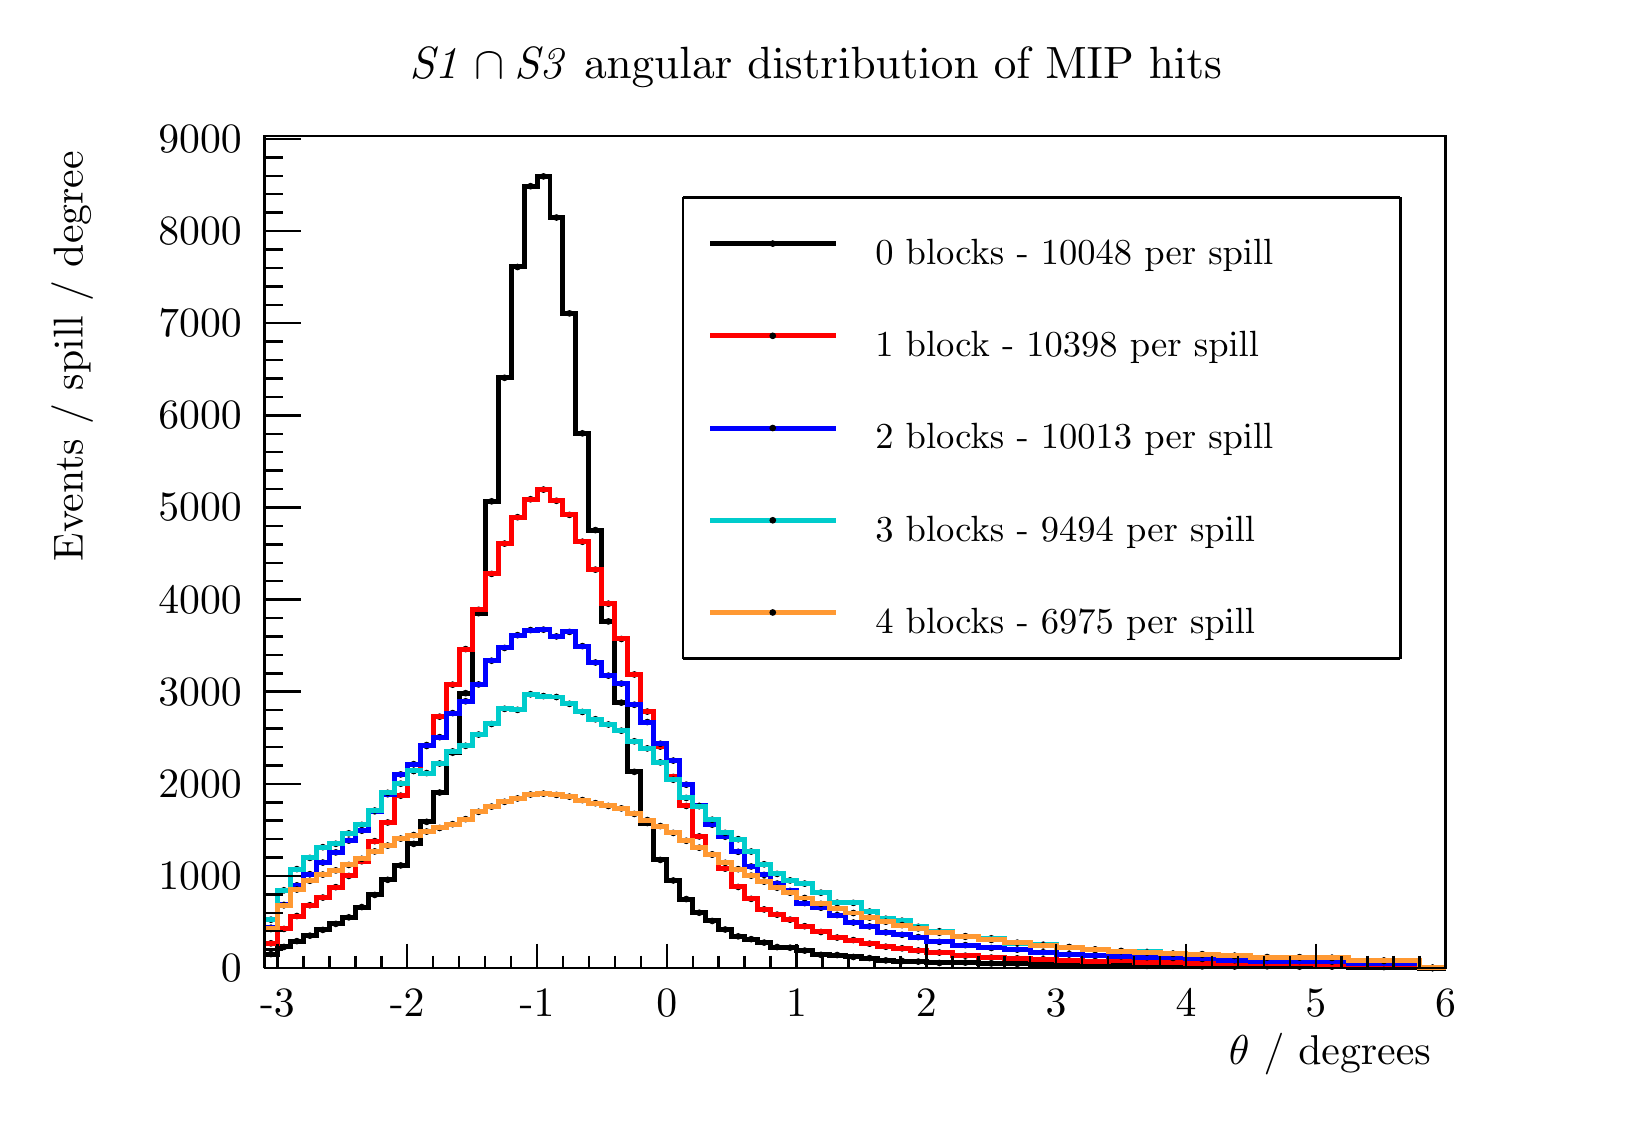
\begin{tikzpicture}
\pgfdeclareplotmark{cross} {
\pgfpathmoveto{\pgfpoint{-0.3\pgfplotmarksize}{\pgfplotmarksize}}
\pgfpathlineto{\pgfpoint{+0.3\pgfplotmarksize}{\pgfplotmarksize}}
\pgfpathlineto{\pgfpoint{+0.3\pgfplotmarksize}{0.3\pgfplotmarksize}}
\pgfpathlineto{\pgfpoint{+1\pgfplotmarksize}{0.3\pgfplotmarksize}}
\pgfpathlineto{\pgfpoint{+1\pgfplotmarksize}{-0.3\pgfplotmarksize}}
\pgfpathlineto{\pgfpoint{+0.3\pgfplotmarksize}{-0.3\pgfplotmarksize}}
\pgfpathlineto{\pgfpoint{+0.3\pgfplotmarksize}{-1.\pgfplotmarksize}}
\pgfpathlineto{\pgfpoint{-0.3\pgfplotmarksize}{-1.\pgfplotmarksize}}
\pgfpathlineto{\pgfpoint{-0.3\pgfplotmarksize}{-0.3\pgfplotmarksize}}
\pgfpathlineto{\pgfpoint{-1.\pgfplotmarksize}{-0.3\pgfplotmarksize}}
\pgfpathlineto{\pgfpoint{-1.\pgfplotmarksize}{0.3\pgfplotmarksize}}
\pgfpathlineto{\pgfpoint{-0.3\pgfplotmarksize}{0.3\pgfplotmarksize}}
\pgfpathclose
\pgfusepathqstroke
}
\pgfdeclareplotmark{cross*} {
\pgfpathmoveto{\pgfpoint{-0.3\pgfplotmarksize}{\pgfplotmarksize}}
\pgfpathlineto{\pgfpoint{+0.3\pgfplotmarksize}{\pgfplotmarksize}}
\pgfpathlineto{\pgfpoint{+0.3\pgfplotmarksize}{0.3\pgfplotmarksize}}
\pgfpathlineto{\pgfpoint{+1\pgfplotmarksize}{0.3\pgfplotmarksize}}
\pgfpathlineto{\pgfpoint{+1\pgfplotmarksize}{-0.3\pgfplotmarksize}}
\pgfpathlineto{\pgfpoint{+0.3\pgfplotmarksize}{-0.3\pgfplotmarksize}}
\pgfpathlineto{\pgfpoint{+0.3\pgfplotmarksize}{-1.\pgfplotmarksize}}
\pgfpathlineto{\pgfpoint{-0.3\pgfplotmarksize}{-1.\pgfplotmarksize}}
\pgfpathlineto{\pgfpoint{-0.3\pgfplotmarksize}{-0.3\pgfplotmarksize}}
\pgfpathlineto{\pgfpoint{-1.\pgfplotmarksize}{-0.3\pgfplotmarksize}}
\pgfpathlineto{\pgfpoint{-1.\pgfplotmarksize}{0.3\pgfplotmarksize}}
\pgfpathlineto{\pgfpoint{-0.3\pgfplotmarksize}{0.3\pgfplotmarksize}}
\pgfpathclose
\pgfusepathqfillstroke
}
\pgfdeclareplotmark{newstar} {
\pgfpathmoveto{\pgfqpoint{0pt}{\pgfplotmarksize}}
\pgfpathlineto{\pgfqpointpolar{44}{0.5\pgfplotmarksize}}
\pgfpathlineto{\pgfqpointpolar{18}{\pgfplotmarksize}}
\pgfpathlineto{\pgfqpointpolar{-20}{0.5\pgfplotmarksize}}
\pgfpathlineto{\pgfqpointpolar{-54}{\pgfplotmarksize}}
\pgfpathlineto{\pgfqpointpolar{-90}{0.5\pgfplotmarksize}}
\pgfpathlineto{\pgfqpointpolar{234}{\pgfplotmarksize}}
\pgfpathlineto{\pgfqpointpolar{198}{0.5\pgfplotmarksize}}
\pgfpathlineto{\pgfqpointpolar{162}{\pgfplotmarksize}}
\pgfpathlineto{\pgfqpointpolar{134}{0.5\pgfplotmarksize}}
\pgfpathclose
\pgfusepathqstroke
}
\pgfdeclareplotmark{newstar*} {
\pgfpathmoveto{\pgfqpoint{0pt}{\pgfplotmarksize}}
\pgfpathlineto{\pgfqpointpolar{44}{0.5\pgfplotmarksize}}
\pgfpathlineto{\pgfqpointpolar{18}{\pgfplotmarksize}}
\pgfpathlineto{\pgfqpointpolar{-20}{0.5\pgfplotmarksize}}
\pgfpathlineto{\pgfqpointpolar{-54}{\pgfplotmarksize}}
\pgfpathlineto{\pgfqpointpolar{-90}{0.5\pgfplotmarksize}}
\pgfpathlineto{\pgfqpointpolar{234}{\pgfplotmarksize}}
\pgfpathlineto{\pgfqpointpolar{198}{0.5\pgfplotmarksize}}
\pgfpathlineto{\pgfqpointpolar{162}{\pgfplotmarksize}}
\pgfpathlineto{\pgfqpointpolar{134}{0.5\pgfplotmarksize}}
\pgfpathclose
\pgfusepathqfillstroke
}
\definecolor{c}{rgb}{1,1,1};
\draw [color=c, fill=c] (0,0) rectangle (20,13.7199);
\draw [color=c, fill=c] (3,1.78359) rectangle (18,12.3479);
\definecolor{c}{rgb}{0,0,0};
\draw [c,line width=0.9] (3,1.78359) -- (3,12.3479) -- (18,12.3479) -- (18,1.78359) -- (3,1.78359);
\definecolor{c}{rgb}{1,1,1};
\draw [color=c, fill=c] (3,1.78359) rectangle (18,12.3479);
\definecolor{c}{rgb}{0,0,0};
\draw [c,line width=0.9] (3,1.78359) -- (3,12.3479) -- (18,12.3479) -- (18,1.78359) -- (3,1.78359);
\definecolor{c}{rgb}{0,0,0.6};
\draw [c,line width=0.9] (3,1.78359) -- (3.16484,1.78359) -- (3.16484,1.78359) -- (3.32967,1.78359) -- (3.32967,1.78359) -- (3.49451,1.78359) -- (3.49451,1.78359) -- (3.65934,1.78359) -- (3.65934,1.78359) -- (3.82418,1.78359) -- (3.82418,1.78359) --
 (3.98901,1.78359) -- (3.98901,1.78359) -- (4.15385,1.78359) -- (4.15385,1.78359) -- (4.31868,1.78359) -- (4.31868,1.78359) -- (4.48352,1.78359) -- (4.48352,1.78359) -- (4.64835,1.78359) -- (4.64835,1.78359) -- (4.81319,1.78359) -- (4.81319,1.78359)
 -- (4.97802,1.78359) -- (4.97802,1.78359) -- (5.14286,1.78359) -- (5.14286,1.78359) -- (5.30769,1.78359) -- (5.30769,1.78359) -- (5.47253,1.78359) -- (5.47253,1.78359) -- (5.63736,1.78359) -- (5.63736,1.78359) -- (5.8022,1.78359) -- (5.8022,1.78359)
 -- (5.96703,1.78359) -- (5.96703,1.78359) -- (6.13187,1.78359) -- (6.13187,1.78359) -- (6.2967,1.78359) -- (6.2967,1.78359) -- (6.46154,1.78359) -- (6.46154,1.78359) -- (6.62637,1.78359) -- (6.62637,1.78359) -- (6.79121,1.78359) -- (6.79121,1.78359)
 -- (6.95604,1.78359) -- (6.95604,1.78359) -- (7.12088,1.78359) -- (7.12088,1.78359) -- (7.28571,1.78359) -- (7.28571,1.78359) -- (7.45055,1.78359) -- (7.45055,1.78359) -- (7.61538,1.78359) -- (7.61538,1.78359) -- (7.78022,1.78359) --
 (7.78022,1.78359) -- (7.94506,1.78359) -- (7.94506,1.78359) -- (8.10989,1.78359) -- (8.10989,1.78359) -- (8.27472,1.78359) -- (8.27472,1.78359) -- (8.43956,1.78359) -- (8.43956,1.78359) -- (8.6044,1.78359) -- (8.6044,1.78359) -- (8.76923,1.78359) --
 (8.76923,1.78359) -- (8.93407,1.78359) -- (8.93407,1.78359) -- (9.0989,1.78359) -- (9.0989,1.78359) -- (9.26374,1.78359) -- (9.26374,1.78359) -- (9.42857,1.78359) -- (9.42857,1.78359) -- (9.59341,1.78359) -- (9.59341,1.78359) -- (9.75824,1.78359) --
 (9.75824,1.78359) -- (9.96429,1.78359) -- (9.96429,1.78359) -- (10.1703,1.78359) -- (10.1703,1.78359) -- (10.3764,1.78359) -- (10.3764,1.78359) -- (10.5824,1.78359) -- (10.5824,1.78359) -- (10.7885,1.78359) -- (10.7885,1.78359) -- (10.9945,1.78359)
 -- (10.9945,1.78359) -- (11.2005,1.78359) -- (11.2005,1.78359) -- (11.4066,1.78359) -- (11.4066,1.78359) -- (11.7363,1.78359) -- (11.7363,1.78359) -- (12.0659,1.78359) -- (12.0659,1.78359) -- (12.3956,1.78359) -- (12.3956,1.78359) --
 (12.7253,1.78359) -- (12.7253,1.78359) -- (13.0549,1.78359) -- (13.0549,1.78359) -- (13.3846,1.78359) -- (13.3846,1.78359) -- (13.7143,1.78359) -- (13.7143,1.78359) -- (14.044,1.78359) -- (14.044,1.78359) -- (14.3736,1.78359) -- (14.3736,1.78359) --
 (14.7033,1.78359) -- (14.7033,1.78359) -- (15.1154,1.78359) -- (15.1154,1.78359) -- (15.5275,1.78359) -- (15.5275,1.78359) -- (15.9396,1.78359) -- (15.9396,1.78359) -- (16.3516,1.78359) -- (16.3516,1.78359) -- (16.7637,1.78359) -- (16.7637,1.78359)
 -- (17.6703,1.78359) -- (17.6703,1.78359) -- (18,1.78359);
\definecolor{c}{rgb}{0,0,0};
\draw [c,line width=0.9] (3,1.78359) -- (18,1.78359);
\draw [c,line width=0.9] (3.16484,2.09229) -- (3.16484,1.78359);
\draw [c,line width=0.9] (3.49451,1.93794) -- (3.49451,1.78359);
\draw [c,line width=0.9] (3.82418,1.93794) -- (3.82418,1.78359);
\draw [c,line width=0.9] (4.15385,1.93794) -- (4.15385,1.78359);
\draw [c,line width=0.9] (4.48352,1.93794) -- (4.48352,1.78359);
\draw [c,line width=0.9] (4.81319,2.09229) -- (4.81319,1.78359);
\draw [c,line width=0.9] (5.14286,1.93794) -- (5.14286,1.78359);
\draw [c,line width=0.9] (5.47253,1.93794) -- (5.47253,1.78359);
\draw [c,line width=0.9] (5.8022,1.93794) -- (5.8022,1.78359);
\draw [c,line width=0.9] (6.13187,1.93794) -- (6.13187,1.78359);
\draw [c,line width=0.9] (6.46154,2.09229) -- (6.46154,1.78359);
\draw [c,line width=0.9] (6.79121,1.93794) -- (6.79121,1.78359);
\draw [c,line width=0.9] (7.12088,1.93794) -- (7.12088,1.78359);
\draw [c,line width=0.9] (7.45055,1.93794) -- (7.45055,1.78359);
\draw [c,line width=0.9] (7.78022,1.93794) -- (7.78022,1.78359);
\draw [c,line width=0.9] (8.10989,2.09229) -- (8.10989,1.78359);
\draw [c,line width=0.9] (8.43956,1.93794) -- (8.43956,1.78359);
\draw [c,line width=0.9] (8.76923,1.93794) -- (8.76923,1.78359);
\draw [c,line width=0.9] (9.0989,1.93794) -- (9.0989,1.78359);
\draw [c,line width=0.9] (9.42857,1.93794) -- (9.42857,1.78359);
\draw [c,line width=0.9] (9.75824,2.09229) -- (9.75824,1.78359);
\draw [c,line width=0.9] (10.0879,1.93794) -- (10.0879,1.78359);
\draw [c,line width=0.9] (10.4176,1.93794) -- (10.4176,1.78359);
\draw [c,line width=0.9] (10.7473,1.93794) -- (10.7473,1.78359);
\draw [c,line width=0.9] (11.0769,1.93794) -- (11.0769,1.78359);
\draw [c,line width=0.9] (11.4066,2.09229) -- (11.4066,1.78359);
\draw [c,line width=0.9] (11.7363,1.93794) -- (11.7363,1.78359);
\draw [c,line width=0.9] (12.0659,1.93794) -- (12.0659,1.78359);
\draw [c,line width=0.9] (12.3956,1.93794) -- (12.3956,1.78359);
\draw [c,line width=0.9] (12.7253,1.93794) -- (12.7253,1.78359);
\draw [c,line width=0.9] (13.0549,2.09229) -- (13.0549,1.78359);
\draw [c,line width=0.9] (13.3846,1.93794) -- (13.3846,1.78359);
\draw [c,line width=0.9] (13.7143,1.93794) -- (13.7143,1.78359);
\draw [c,line width=0.9] (14.044,1.93794) -- (14.044,1.78359);
\draw [c,line width=0.9] (14.3736,1.93794) -- (14.3736,1.78359);
\draw [c,line width=0.9] (14.7033,2.09229) -- (14.7033,1.78359);
\draw [c,line width=0.9] (15.033,1.93794) -- (15.033,1.78359);
\draw [c,line width=0.9] (15.3626,1.93794) -- (15.3626,1.78359);
\draw [c,line width=0.9] (15.6923,1.93794) -- (15.6923,1.78359);
\draw [c,line width=0.9] (16.022,1.93794) -- (16.022,1.78359);
\draw [c,line width=0.9] (16.3516,2.09229) -- (16.3516,1.78359);
\draw [c,line width=0.9] (16.6813,1.93794) -- (16.6813,1.78359);
\draw [c,line width=0.9] (17.011,1.93794) -- (17.011,1.78359);
\draw [c,line width=0.9] (17.3407,1.93794) -- (17.3407,1.78359);
\draw [c,line width=0.9] (17.6703,1.93794) -- (17.6703,1.78359);
\draw [c,line width=0.9] (18,2.09229) -- (18,1.78359);
\draw [c,line width=0.9] (3.16484,2.09229) -- (3.16484,1.78359);
\draw [anchor=base] (3.16484,1.1662) node[scale=1.50787, color=c, rotate=0]{-3};
\draw [anchor=base] (4.81319,1.1662) node[scale=1.50787, color=c, rotate=0]{-2};
\draw [anchor=base] (6.46154,1.1662) node[scale=1.50787, color=c, rotate=0]{-1};
\draw [anchor=base] (8.10989,1.1662) node[scale=1.50787, color=c, rotate=0]{0};
\draw [anchor=base] (9.75824,1.1662) node[scale=1.50787, color=c, rotate=0]{1};
\draw [anchor=base] (11.4066,1.1662) node[scale=1.50787, color=c, rotate=0]{2};
\draw [anchor=base] (13.0549,1.1662) node[scale=1.50787, color=c, rotate=0]{3};
\draw [anchor=base] (14.7033,1.1662) node[scale=1.50787, color=c, rotate=0]{4};
\draw [anchor=base] (16.3516,1.1662) node[scale=1.50787, color=c, rotate=0]{5};
\draw [anchor=base] (18,1.1662) node[scale=1.50787, color=c, rotate=0]{6};
\draw [anchor= east] (18,0.685997) node[scale=1.50787, color=c, rotate=0]{$\theta$ / degrees};
\draw [c,line width=0.9] (3,1.78359) -- (3,12.3479);
\draw [c,line width=0.9] (3.462,1.78359) -- (3,1.78359);
\draw [c,line width=0.9] (3.231,2.01758) -- (3,2.01758);
\draw [c,line width=0.9] (3.231,2.25157) -- (3,2.25157);
\draw [c,line width=0.9] (3.231,2.48557) -- (3,2.48557);
\draw [c,line width=0.9] (3.231,2.71956) -- (3,2.71956);
\draw [c,line width=0.9] (3.462,2.95355) -- (3,2.95355);
\draw [c,line width=0.9] (3.231,3.18754) -- (3,3.18754);
\draw [c,line width=0.9] (3.231,3.42153) -- (3,3.42153);
\draw [c,line width=0.9] (3.231,3.65552) -- (3,3.65552);
\draw [c,line width=0.9] (3.231,3.88951) -- (3,3.88951);
\draw [c,line width=0.9] (3.462,4.1235) -- (3,4.1235);
\draw [c,line width=0.9] (3.231,4.35749) -- (3,4.35749);
\draw [c,line width=0.9] (3.231,4.59148) -- (3,4.59148);
\draw [c,line width=0.9] (3.231,4.82548) -- (3,4.82548);
\draw [c,line width=0.9] (3.231,5.05947) -- (3,5.05947);
\draw [c,line width=0.9] (3.462,5.29346) -- (3,5.29346);
\draw [c,line width=0.9] (3.231,5.52745) -- (3,5.52745);
\draw [c,line width=0.9] (3.231,5.76144) -- (3,5.76144);
\draw [c,line width=0.9] (3.231,5.99543) -- (3,5.99543);
\draw [c,line width=0.9] (3.231,6.22942) -- (3,6.22942);
\draw [c,line width=0.9] (3.462,6.46341) -- (3,6.46341);
\draw [c,line width=0.9] (3.231,6.6974) -- (3,6.6974);
\draw [c,line width=0.9] (3.231,6.93139) -- (3,6.93139);
\draw [c,line width=0.9] (3.231,7.16539) -- (3,7.16539);
\draw [c,line width=0.9] (3.231,7.39938) -- (3,7.39938);
\draw [c,line width=0.9] (3.462,7.63337) -- (3,7.63337);
\draw [c,line width=0.9] (3.231,7.86736) -- (3,7.86736);
\draw [c,line width=0.9] (3.231,8.10135) -- (3,8.10135);
\draw [c,line width=0.9] (3.231,8.33534) -- (3,8.33534);
\draw [c,line width=0.9] (3.231,8.56933) -- (3,8.56933);
\draw [c,line width=0.9] (3.462,8.80332) -- (3,8.80332);
\draw [c,line width=0.9] (3.231,9.03731) -- (3,9.03731);
\draw [c,line width=0.9] (3.231,9.27131) -- (3,9.27131);
\draw [c,line width=0.9] (3.231,9.5053) -- (3,9.5053);
\draw [c,line width=0.9] (3.231,9.73929) -- (3,9.73929);
\draw [c,line width=0.9] (3.462,9.97328) -- (3,9.97328);
\draw [c,line width=0.9] (3.231,10.2073) -- (3,10.2073);
\draw [c,line width=0.9] (3.231,10.4413) -- (3,10.4413);
\draw [c,line width=0.9] (3.231,10.6753) -- (3,10.6753);
\draw [c,line width=0.9] (3.231,10.9092) -- (3,10.9092);
\draw [c,line width=0.9] (3.462,11.1432) -- (3,11.1432);
\draw [c,line width=0.9] (3.231,11.3772) -- (3,11.3772);
\draw [c,line width=0.9] (3.231,11.6112) -- (3,11.6112);
\draw [c,line width=0.9] (3.231,11.8452) -- (3,11.8452);
\draw [c,line width=0.9] (3.231,12.0792) -- (3,12.0792);
\draw [c,line width=0.9] (3.462,12.3132) -- (3,12.3132);
\draw [c,line width=0.9] (3.462,12.3132) -- (3,12.3132);
\draw [anchor= east] (2.9,1.78359) node[scale=1.50787, color=c, rotate=0]{0};
\draw [anchor= east] (2.9,2.95355) node[scale=1.50787, color=c, rotate=0]{1000};
\draw [anchor= east] (2.9,4.1235) node[scale=1.50787, color=c, rotate=0]{2000};
\draw [anchor= east] (2.9,5.29346) node[scale=1.50787, color=c, rotate=0]{3000};
\draw [anchor= east] (2.9,6.46341) node[scale=1.50787, color=c, rotate=0]{4000};
\draw [anchor= east] (2.9,7.63337) node[scale=1.50787, color=c, rotate=0]{5000};
\draw [anchor= east] (2.9,8.80332) node[scale=1.50787, color=c, rotate=0]{6000};
\draw [anchor= east] (2.9,9.97328) node[scale=1.50787, color=c, rotate=0]{7000};
\draw [anchor= east] (2.9,11.1432) node[scale=1.50787, color=c, rotate=0]{8000};
\draw [anchor= east] (2.9,12.3132) node[scale=1.50787, color=c, rotate=0]{9000};
\draw [anchor= east] (0.557284,12.3479) node[scale=1.50787, color=c, rotate=90]{ Events / spill / degree};
\draw [c,line width=1.8] (3.08242,1.96042) -- (3.08242,1.96133);
\draw [c,line width=1.8] (3.08242,1.96133) -- (3.08242,1.96225);
\foreach \P in {(3.08242,1.96133)}{\draw[mark options={color=c,fill=c},mark size=2.402402pt,mark=*,mark size=1pt] plot coordinates {\P};}
\draw [c,line width=1.8] (3.24725,2.05096) -- (3.24725,2.05209);
\draw [c,line width=1.8] (3.24725,2.05209) -- (3.24725,2.05321);
\foreach \P in {(3.24725,2.05209)}{\draw[mark options={color=c,fill=c},mark size=2.402402pt,mark=*,mark size=1pt] plot coordinates {\P};}
\draw [c,line width=1.8] (3.41209,2.1247) -- (3.41209,2.12597);
\draw [c,line width=1.8] (3.41209,2.12597) -- (3.41209,2.12724);
\foreach \P in {(3.41209,2.12597)}{\draw[mark options={color=c,fill=c},mark size=2.402402pt,mark=*,mark size=1pt] plot coordinates {\P};}
\draw [c,line width=1.8] (3.57692,2.19382) -- (3.57692,2.19522);
\draw [c,line width=1.8] (3.57692,2.19522) -- (3.57692,2.19662);
\foreach \P in {(3.57692,2.19522)}{\draw[mark options={color=c,fill=c},mark size=2.402402pt,mark=*,mark size=1pt] plot coordinates {\P};}
\draw [c,line width=1.8] (3.74176,2.26714) -- (3.74176,2.26865);
\draw [c,line width=1.8] (3.74176,2.26865) -- (3.74176,2.27017);
\foreach \P in {(3.74176,2.26865)}{\draw[mark options={color=c,fill=c},mark size=2.402402pt,mark=*,mark size=1pt] plot coordinates {\P};}
\draw [c,line width=1.8] (3.90659,2.34336) -- (3.90659,2.34499);
\draw [c,line width=1.8] (3.90659,2.34499) -- (3.90659,2.34662);
\foreach \P in {(3.90659,2.34499)}{\draw[mark options={color=c,fill=c},mark size=2.402402pt,mark=*,mark size=1pt] plot coordinates {\P};}
\draw [c,line width=1.8] (4.07143,2.42657) -- (4.07143,2.42831);
\draw [c,line width=1.8] (4.07143,2.42831) -- (4.07143,2.43004);
\foreach \P in {(4.07143,2.42831)}{\draw[mark options={color=c,fill=c},mark size=2.402402pt,mark=*,mark size=1pt] plot coordinates {\P};}
\draw [c,line width=1.8] (4.23626,2.55668) -- (4.23626,2.55859);
\draw [c,line width=1.8] (4.23626,2.55859) -- (4.23626,2.5605);
\foreach \P in {(4.23626,2.55859)}{\draw[mark options={color=c,fill=c},mark size=2.402402pt,mark=*,mark size=1pt] plot coordinates {\P};}
\draw [c,line width=1.8] (4.4011,2.71038) -- (4.4011,2.71247);
\draw [c,line width=1.8] (4.4011,2.71247) -- (4.4011,2.71456);
\foreach \P in {(4.4011,2.71247)}{\draw[mark options={color=c,fill=c},mark size=2.402402pt,mark=*,mark size=1pt] plot coordinates {\P};}
\draw [c,line width=1.8] (4.56593,2.90221) -- (4.56593,2.90451);
\draw [c,line width=1.8] (4.56593,2.90451) -- (4.56593,2.90682);
\foreach \P in {(4.56593,2.90451)}{\draw[mark options={color=c,fill=c},mark size=2.402402pt,mark=*,mark size=1pt] plot coordinates {\P};}
\draw [c,line width=1.8] (4.73077,3.08496) -- (4.73077,3.08744);
\draw [c,line width=1.8] (4.73077,3.08744) -- (4.73077,3.08992);
\foreach \P in {(4.73077,3.08744)}{\draw[mark options={color=c,fill=c},mark size=2.402402pt,mark=*,mark size=1pt] plot coordinates {\P};}
\draw [c,line width=1.8] (4.8956,3.35822) -- (4.8956,3.36094);
\draw [c,line width=1.8] (4.8956,3.36094) -- (4.8956,3.36367);
\foreach \P in {(4.8956,3.36094)}{\draw[mark options={color=c,fill=c},mark size=2.402402pt,mark=*,mark size=1pt] plot coordinates {\P};}
\draw [c,line width=1.8] (5.06044,3.63804) -- (5.06044,3.641);
\draw [c,line width=1.8] (5.06044,3.641) -- (5.06044,3.64396);
\foreach \P in {(5.06044,3.641)}{\draw[mark options={color=c,fill=c},mark size=2.402402pt,mark=*,mark size=1pt] plot coordinates {\P};}
\draw [c,line width=1.8] (5.22528,4.00993) -- (5.22528,4.01317);
\draw [c,line width=1.8] (5.22528,4.01317) -- (5.22528,4.01641);
\foreach \P in {(5.22528,4.01317)}{\draw[mark options={color=c,fill=c},mark size=2.402402pt,mark=*,mark size=1pt] plot coordinates {\P};}
\draw [c,line width=1.8] (5.39011,4.5153) -- (5.39011,4.5189);
\draw [c,line width=1.8] (5.39011,4.5189) -- (5.39011,4.52249);
\foreach \P in {(5.39011,4.5189)}{\draw[mark options={color=c,fill=c},mark size=2.402402pt,mark=*,mark size=1pt] plot coordinates {\P};}
\draw [c,line width=1.8] (5.55494,5.27113) -- (5.55494,5.27519);
\draw [c,line width=1.8] (5.55494,5.27519) -- (5.55494,5.27926);
\foreach \P in {(5.55494,5.27519)}{\draw[mark options={color=c,fill=c},mark size=2.402402pt,mark=*,mark size=1pt] plot coordinates {\P};}
\draw [c,line width=1.8] (5.71978,6.28683) -- (5.71978,6.29145);
\draw [c,line width=1.8] (5.71978,6.29145) -- (5.71978,6.29606);
\foreach \P in {(5.71978,6.29145)}{\draw[mark options={color=c,fill=c},mark size=2.402402pt,mark=*,mark size=1pt] plot coordinates {\P};}
\draw [c,line width=1.8] (5.88462,7.70618) -- (5.88462,7.71147);
\draw [c,line width=1.8] (5.88462,7.71147) -- (5.88462,7.71676);
\foreach \P in {(5.88462,7.71147)}{\draw[mark options={color=c,fill=c},mark size=2.402402pt,mark=*,mark size=1pt] plot coordinates {\P};}
\draw [c,line width=1.8] (6.04945,9.27429) -- (6.04945,9.28024);
\draw [c,line width=1.8] (6.04945,9.28024) -- (6.04945,9.28619);
\foreach \P in {(6.04945,9.28024)}{\draw[mark options={color=c,fill=c},mark size=2.402402pt,mark=*,mark size=1pt] plot coordinates {\P};}
\draw [c,line width=1.8] (6.21429,10.681) -- (6.21429,10.6875);
\draw [c,line width=1.8] (6.21429,10.6875) -- (6.21429,10.694);
\foreach \P in {(6.21429,10.6875)}{\draw[mark options={color=c,fill=c},mark size=2.402402pt,mark=*,mark size=1pt] plot coordinates {\P};}
\draw [c,line width=1.8] (6.37912,11.7069) -- (6.37912,11.7137);
\draw [c,line width=1.8] (6.37912,11.7137) -- (6.37912,11.7206);
\foreach \P in {(6.37912,11.7137)}{\draw[mark options={color=c,fill=c},mark size=2.402402pt,mark=*,mark size=1pt] plot coordinates {\P};}
\draw [c,line width=1.8] (6.54396,11.8311) -- (6.54396,11.838);
\draw [c,line width=1.8] (6.54396,11.838) -- (6.54396,11.8449);
\foreach \P in {(6.54396,11.838)}{\draw[mark options={color=c,fill=c},mark size=2.402402pt,mark=*,mark size=1pt] plot coordinates {\P};}
\draw [c,line width=1.8] (6.70879,11.3088) -- (6.70879,11.3155);
\draw [c,line width=1.8] (6.70879,11.3155) -- (6.70879,11.3222);
\foreach \P in {(6.70879,11.3155)}{\draw[mark options={color=c,fill=c},mark size=2.402402pt,mark=*,mark size=1pt] plot coordinates {\P};}
\draw [c,line width=1.8] (6.87363,10.0921) -- (6.87363,10.0984);
\draw [c,line width=1.8] (6.87363,10.0984) -- (6.87363,10.1047);
\foreach \P in {(6.87363,10.0984)}{\draw[mark options={color=c,fill=c},mark size=2.402402pt,mark=*,mark size=1pt] plot coordinates {\P};}
\draw [c,line width=1.8] (7.03846,8.56933) -- (7.03846,8.575);
\draw [c,line width=1.8] (7.03846,8.575) -- (7.03846,8.58066);
\foreach \P in {(7.03846,8.575)}{\draw[mark options={color=c,fill=c},mark size=2.402402pt,mark=*,mark size=1pt] plot coordinates {\P};}
\draw [c,line width=1.8] (7.2033,7.34089) -- (7.2033,7.34602);
\draw [c,line width=1.8] (7.2033,7.34602) -- (7.2033,7.35115);
\foreach \P in {(7.2033,7.34602)}{\draw[mark options={color=c,fill=c},mark size=2.402402pt,mark=*,mark size=1pt] plot coordinates {\P};}
\draw [c,line width=1.8] (7.36813,6.1819) -- (7.36813,6.18646);
\draw [c,line width=1.8] (7.36813,6.18646) -- (7.36813,6.19101);
\foreach \P in {(7.36813,6.18646)}{\draw[mark options={color=c,fill=c},mark size=2.402402pt,mark=*,mark size=1pt] plot coordinates {\P};}
\draw [c,line width=1.8] (7.53297,5.15058) -- (7.53297,5.15457);
\draw [c,line width=1.8] (7.53297,5.15457) -- (7.53297,5.15856);
\foreach \P in {(7.53297,5.15457)}{\draw[mark options={color=c,fill=c},mark size=2.402402pt,mark=*,mark size=1pt] plot coordinates {\P};}
\draw [c,line width=1.8] (7.6978,4.27259) -- (7.6978,4.27602);
\draw [c,line width=1.8] (7.6978,4.27602) -- (7.6978,4.27944);
\foreach \P in {(7.6978,4.27602)}{\draw[mark options={color=c,fill=c},mark size=2.402402pt,mark=*,mark size=1pt] plot coordinates {\P};}
\draw [c,line width=1.8] (7.86264,3.62309) -- (7.86264,3.62604);
\draw [c,line width=1.8] (7.86264,3.62604) -- (7.86264,3.62899);
\foreach \P in {(7.86264,3.62604)}{\draw[mark options={color=c,fill=c},mark size=2.402402pt,mark=*,mark size=1pt] plot coordinates {\P};}
\draw [c,line width=1.8] (8.02747,3.15496) -- (8.02747,3.15751);
\draw [c,line width=1.8] (8.02747,3.15751) -- (8.02747,3.16006);
\foreach \P in {(8.02747,3.15751)}{\draw[mark options={color=c,fill=c},mark size=2.402402pt,mark=*,mark size=1pt] plot coordinates {\P};}
\draw [c,line width=1.8] (8.19231,2.89398) -- (8.19231,2.89627);
\draw [c,line width=1.8] (8.19231,2.89627) -- (8.19231,2.89856);
\foreach \P in {(8.19231,2.89627)}{\draw[mark options={color=c,fill=c},mark size=2.402402pt,mark=*,mark size=1pt] plot coordinates {\P};}
\draw [c,line width=1.8] (8.35714,2.65818) -- (8.35714,2.66022);
\draw [c,line width=1.8] (8.35714,2.66022) -- (8.35714,2.66225);
\foreach \P in {(8.35714,2.66022)}{\draw[mark options={color=c,fill=c},mark size=2.402402pt,mark=*,mark size=1pt] plot coordinates {\P};}
\draw [c,line width=1.8] (8.52198,2.48491) -- (8.52198,2.48674);
\draw [c,line width=1.8] (8.52198,2.48674) -- (8.52198,2.48857);
\foreach \P in {(8.52198,2.48674)}{\draw[mark options={color=c,fill=c},mark size=2.402402pt,mark=*,mark size=1pt] plot coordinates {\P};}
\draw [c,line width=1.8] (8.68681,2.38063) -- (8.68681,2.38232);
\draw [c,line width=1.8] (8.68681,2.38232) -- (8.68681,2.384);
\foreach \P in {(8.68681,2.38232)}{\draw[mark options={color=c,fill=c},mark size=2.402402pt,mark=*,mark size=1pt] plot coordinates {\P};}
\draw [c,line width=1.8] (8.85165,2.272) -- (8.85165,2.27352);
\draw [c,line width=1.8] (8.85165,2.27352) -- (8.85165,2.27504);
\foreach \P in {(8.85165,2.27352)}{\draw[mark options={color=c,fill=c},mark size=2.402402pt,mark=*,mark size=1pt] plot coordinates {\P};}
\draw [c,line width=1.8] (9.01648,2.18553) -- (9.01648,2.18691);
\draw [c,line width=1.8] (9.01648,2.18691) -- (9.01648,2.1883);
\foreach \P in {(9.01648,2.18691)}{\draw[mark options={color=c,fill=c},mark size=2.402402pt,mark=*,mark size=1pt] plot coordinates {\P};}
\draw [c,line width=1.8] (9.18132,2.14992) -- (9.18132,2.15123);
\draw [c,line width=1.8] (9.18132,2.15123) -- (9.18132,2.15255);
\foreach \P in {(9.18132,2.15123)}{\draw[mark options={color=c,fill=c},mark size=2.402402pt,mark=*,mark size=1pt] plot coordinates {\P};}
\draw [c,line width=1.8] (9.34615,2.10613) -- (9.34615,2.10737);
\draw [c,line width=1.8] (9.34615,2.10737) -- (9.34615,2.10861);
\foreach \P in {(9.34615,2.10737)}{\draw[mark options={color=c,fill=c},mark size=2.402402pt,mark=*,mark size=1pt] plot coordinates {\P};}
\draw [c,line width=1.8] (9.51099,2.04971) -- (9.51099,2.05084);
\draw [c,line width=1.8] (9.51099,2.05084) -- (9.51099,2.05196);
\foreach \P in {(9.51099,2.05084)}{\draw[mark options={color=c,fill=c},mark size=2.402402pt,mark=*,mark size=1pt] plot coordinates {\P};}
\draw [c,line width=1.8] (9.67582,2.04139) -- (9.67582,2.0425);
\draw [c,line width=1.8] (9.67582,2.0425) -- (9.67582,2.04362);
\foreach \P in {(9.67582,2.0425)}{\draw[mark options={color=c,fill=c},mark size=2.402402pt,mark=*,mark size=1pt] plot coordinates {\P};}
\draw [c,line width=1.8] (9.86126,2.00446) -- (9.86126,2.0056);
\draw [c,line width=1.8] (9.86126,2.0056) -- (9.86126,2.00675);
\foreach \P in {(9.86126,2.0056)}{\draw[mark options={color=c,fill=c},mark size=2.402402pt,mark=*,mark size=1pt] plot coordinates {\P};}
\draw [c,line width=1.8] (10.0673,1.95095) -- (10.0673,1.95195);
\draw [c,line width=1.8] (10.0673,1.95195) -- (10.0673,1.95295);
\foreach \P in {(10.0673,1.95195)}{\draw[mark options={color=c,fill=c},mark size=2.402402pt,mark=*,mark size=1pt] plot coordinates {\P};}
\draw [c,line width=1.8] (10.2734,1.94837) -- (10.2734,1.94936);
\draw [c,line width=1.8] (10.2734,1.94936) -- (10.2734,1.95035);
\foreach \P in {(10.2734,1.94936)}{\draw[mark options={color=c,fill=c},mark size=2.402402pt,mark=*,mark size=1pt] plot coordinates {\P};}
\draw [c,line width=1.8] (10.4794,1.92407) -- (10.4794,1.92498);
\draw [c,line width=1.8] (10.4794,1.92498) -- (10.4794,1.92589);
\foreach \P in {(10.4794,1.92498)}{\draw[mark options={color=c,fill=c},mark size=2.402402pt,mark=*,mark size=1pt] plot coordinates {\P};}
\draw [c,line width=1.8] (10.6854,1.90959) -- (10.6854,1.91046);
\draw [c,line width=1.8] (10.6854,1.91046) -- (10.6854,1.91133);
\foreach \P in {(10.6854,1.91046)}{\draw[mark options={color=c,fill=c},mark size=2.402402pt,mark=*,mark size=1pt] plot coordinates {\P};}
\draw [c,line width=1.8] (10.8915,1.88035) -- (10.8915,1.88111);
\draw [c,line width=1.8] (10.8915,1.88111) -- (10.8915,1.88187);
\foreach \P in {(10.8915,1.88111)}{\draw[mark options={color=c,fill=c},mark size=2.402402pt,mark=*,mark size=1pt] plot coordinates {\P};}
\draw [c,line width=1.8] (11.0975,1.87278) -- (11.0975,1.87351);
\draw [c,line width=1.8] (11.0975,1.87351) -- (11.0975,1.87424);
\foreach \P in {(11.0975,1.87351)}{\draw[mark options={color=c,fill=c},mark size=2.402402pt,mark=*,mark size=1pt] plot coordinates {\P};}
\draw [c,line width=1.8] (11.3036,1.86516) -- (11.3036,1.86587);
\draw [c,line width=1.8] (11.3036,1.86587) -- (11.3036,1.86657);
\foreach \P in {(11.3036,1.86587)}{\draw[mark options={color=c,fill=c},mark size=2.402402pt,mark=*,mark size=1pt] plot coordinates {\P};}
\draw [c,line width=1.8] (11.5714,1.8481) -- (11.5714,1.84889);
\draw [c,line width=1.8] (11.5714,1.84889) -- (11.5714,1.84967);
\foreach \P in {(11.5714,1.84889)}{\draw[mark options={color=c,fill=c},mark size=2.402402pt,mark=*,mark size=1pt] plot coordinates {\P};}
\draw [c,line width=1.8] (11.9011,1.85223) -- (11.9011,1.85304);
\draw [c,line width=1.8] (11.9011,1.85304) -- (11.9011,1.85385);
\foreach \P in {(11.9011,1.85304)}{\draw[mark options={color=c,fill=c},mark size=2.402402pt,mark=*,mark size=1pt] plot coordinates {\P};}
\draw [c,line width=1.8] (12.2308,1.84206) -- (12.2308,1.84281);
\draw [c,line width=1.8] (12.2308,1.84281) -- (12.2308,1.84356);
\foreach \P in {(12.2308,1.84281)}{\draw[mark options={color=c,fill=c},mark size=2.402402pt,mark=*,mark size=1pt] plot coordinates {\P};}
\draw [c,line width=1.8] (12.5604,1.83622) -- (12.5604,1.83693);
\draw [c,line width=1.8] (12.5604,1.83693) -- (12.5604,1.83764);
\foreach \P in {(12.5604,1.83693)}{\draw[mark options={color=c,fill=c},mark size=2.402402pt,mark=*,mark size=1pt] plot coordinates {\P};}
\draw [c,line width=1.8] (12.8901,1.82585) -- (12.8901,1.82649);
\draw [c,line width=1.8] (12.8901,1.82649) -- (12.8901,1.82713);
\foreach \P in {(12.8901,1.82649)}{\draw[mark options={color=c,fill=c},mark size=2.402402pt,mark=*,mark size=1pt] plot coordinates {\P};}
\draw [c,line width=1.8] (13.2198,1.82341) -- (13.2198,1.82402);
\draw [c,line width=1.8] (13.2198,1.82402) -- (13.2198,1.82464);
\foreach \P in {(13.2198,1.82402)}{\draw[mark options={color=c,fill=c},mark size=2.402402pt,mark=*,mark size=1pt] plot coordinates {\P};}
\draw [c,line width=1.8] (13.5495,1.81898) -- (13.5495,1.81956);
\draw [c,line width=1.8] (13.5495,1.81956) -- (13.5495,1.82014);
\foreach \P in {(13.5495,1.81956)}{\draw[mark options={color=c,fill=c},mark size=2.402402pt,mark=*,mark size=1pt] plot coordinates {\P};}
\draw [c,line width=1.8] (13.8791,1.81696) -- (13.8791,1.81754);
\draw [c,line width=1.8] (13.8791,1.81754) -- (13.8791,1.81812);
\foreach \P in {(13.8791,1.81754)}{\draw[mark options={color=c,fill=c},mark size=2.402402pt,mark=*,mark size=1pt] plot coordinates {\P};}
\draw [c,line width=1.8] (14.2088,1.81084) -- (14.2088,1.81136);
\draw [c,line width=1.8] (14.2088,1.81136) -- (14.2088,1.81187);
\foreach \P in {(14.2088,1.81136)}{\draw[mark options={color=c,fill=c},mark size=2.402402pt,mark=*,mark size=1pt] plot coordinates {\P};}
\draw [c,line width=1.8] (14.5385,1.81226) -- (14.5385,1.81279);
\draw [c,line width=1.8] (14.5385,1.81279) -- (14.5385,1.81331);
\foreach \P in {(14.5385,1.81279)}{\draw[mark options={color=c,fill=c},mark size=2.402402pt,mark=*,mark size=1pt] plot coordinates {\P};}
\draw [c,line width=1.8] (14.9093,1.80551) -- (14.9093,1.80603);
\draw [c,line width=1.8] (14.9093,1.80603) -- (14.9093,1.80656);
\foreach \P in {(14.9093,1.80603)}{\draw[mark options={color=c,fill=c},mark size=2.402402pt,mark=*,mark size=1pt] plot coordinates {\P};}
\draw [c,line width=1.8] (15.3214,1.80324) -- (15.3214,1.80373);
\draw [c,line width=1.8] (15.3214,1.80373) -- (15.3214,1.80421);
\foreach \P in {(15.3214,1.80373)}{\draw[mark options={color=c,fill=c},mark size=2.402402pt,mark=*,mark size=1pt] plot coordinates {\P};}
\draw [c,line width=1.8] (15.7335,1.80624) -- (15.7335,1.80676);
\draw [c,line width=1.8] (15.7335,1.80676) -- (15.7335,1.80729);
\foreach \P in {(15.7335,1.80676)}{\draw[mark options={color=c,fill=c},mark size=2.402402pt,mark=*,mark size=1pt] plot coordinates {\P};}
\draw [c,line width=1.8] (16.1456,1.80134) -- (16.1456,1.8018);
\draw [c,line width=1.8] (16.1456,1.8018) -- (16.1456,1.80227);
\foreach \P in {(16.1456,1.8018)}{\draw[mark options={color=c,fill=c},mark size=2.402402pt,mark=*,mark size=1pt] plot coordinates {\P};}
\draw [c,line width=1.8] (16.5577,1.80172) -- (16.5577,1.80219);
\draw [c,line width=1.8] (16.5577,1.80219) -- (16.5577,1.80265);
\foreach \P in {(16.5577,1.80219)}{\draw[mark options={color=c,fill=c},mark size=2.402402pt,mark=*,mark size=1pt] plot coordinates {\P};}
\draw [c,line width=1.8] (17.217,1.79545) -- (17.217,1.79602);
\draw [c,line width=1.8] (17.217,1.79602) -- (17.217,1.79658);
\foreach \P in {(17.217,1.79602)}{\draw[mark options={color=c,fill=c},mark size=2.402402pt,mark=*,mark size=1pt] plot coordinates {\P};}
\draw [c,line width=1.8] (17.8352,1.78436) -- (17.8352,1.78458);
\draw [c,line width=1.8] (17.8352,1.78458) -- (17.8352,1.7848);
\foreach \P in {(17.8352,1.78458)}{\draw[mark options={color=c,fill=c},mark size=2.402402pt,mark=*,mark size=1pt] plot coordinates {\P};}
\draw [c,line width=1.8] (3,1.96133) -- (3.16484,1.96133) -- (3.16484,2.05209) -- (3.32967,2.05209) -- (3.32967,2.12597) -- (3.49451,2.12597) -- (3.49451,2.19522) -- (3.65934,2.19522) -- (3.65934,2.26865) -- (3.82418,2.26865) -- (3.82418,2.34499) --
 (3.98901,2.34499) -- (3.98901,2.42831) -- (4.15385,2.42831) -- (4.15385,2.55859) -- (4.31868,2.55859) -- (4.31868,2.71247) -- (4.48352,2.71247) -- (4.48352,2.90451) -- (4.64835,2.90451) -- (4.64835,3.08744) -- (4.81319,3.08744) -- (4.81319,3.36094)
 -- (4.97802,3.36094) -- (4.97802,3.641) -- (5.14286,3.641) -- (5.14286,4.01317) -- (5.30769,4.01317) -- (5.30769,4.5189) -- (5.47253,4.5189) -- (5.47253,5.27519) -- (5.63736,5.27519) -- (5.63736,6.29145) -- (5.8022,6.29145) -- (5.8022,7.71147) --
 (5.96703,7.71147) -- (5.96703,9.28024) -- (6.13187,9.28024) -- (6.13187,10.6875) -- (6.2967,10.6875) -- (6.2967,11.7137) -- (6.46154,11.7137) -- (6.46154,11.838) -- (6.62637,11.838) -- (6.62637,11.3155) -- (6.79121,11.3155) -- (6.79121,10.0984) --
 (6.95604,10.0984) -- (6.95604,8.575) -- (7.12088,8.575) -- (7.12088,7.34602) -- (7.28571,7.34602) -- (7.28571,6.18646) -- (7.45055,6.18646) -- (7.45055,5.15457) -- (7.61538,5.15457) -- (7.61538,4.27602) -- (7.78022,4.27602) -- (7.78022,3.62604) --
 (7.94506,3.62604) -- (7.94506,3.15751) -- (8.10989,3.15751) -- (8.10989,2.89627) -- (8.27472,2.89627) -- (8.27472,2.66022) -- (8.43956,2.66022) -- (8.43956,2.48674) -- (8.6044,2.48674) -- (8.6044,2.38232) -- (8.76923,2.38232) -- (8.76923,2.27352) --
 (8.93407,2.27352) -- (8.93407,2.18691) -- (9.0989,2.18691) -- (9.0989,2.15123) -- (9.26374,2.15123) -- (9.26374,2.10737) -- (9.42857,2.10737) -- (9.42857,2.05084) -- (9.59341,2.05084) -- (9.59341,2.0425) -- (9.75824,2.0425) -- (9.75824,2.0056) --
 (9.96429,2.0056) -- (9.96429,1.95195) -- (10.1703,1.95195) -- (10.1703,1.94936) -- (10.3764,1.94936) -- (10.3764,1.92498) -- (10.5824,1.92498) -- (10.5824,1.91046) -- (10.7885,1.91046) -- (10.7885,1.88111) -- (10.9945,1.88111) -- (10.9945,1.87351)
 -- (11.2005,1.87351) -- (11.2005,1.86587) -- (11.4066,1.86587) -- (11.4066,1.84889) -- (11.7363,1.84889) -- (11.7363,1.85304) -- (12.0659,1.85304) -- (12.0659,1.84281) -- (12.3956,1.84281) -- (12.3956,1.83693) -- (12.7253,1.83693) --
 (12.7253,1.82649) -- (13.0549,1.82649) -- (13.0549,1.82402) -- (13.3846,1.82402) -- (13.3846,1.81956) -- (13.7143,1.81956) -- (13.7143,1.81754) -- (14.044,1.81754) -- (14.044,1.81136) -- (14.3736,1.81136) -- (14.3736,1.81279) -- (14.7033,1.81279) --
 (14.7033,1.80603) -- (15.1154,1.80603) -- (15.1154,1.80373) -- (15.5275,1.80373) -- (15.5275,1.80676) -- (15.9396,1.80676) -- (15.9396,1.8018) -- (16.3516,1.8018) -- (16.3516,1.80219) -- (16.7637,1.80219) -- (16.7637,1.79602) -- (17.6703,1.79602) --
 (17.6703,1.78359) -- (18,1.78359);
\definecolor{c}{rgb}{1,0,0};
\draw [c,line width=1.8] (3.08242,2.09714) -- (3.08242,2.09815);
\draw [c,line width=1.8] (3.08242,2.09815) -- (3.08242,2.09916);
\definecolor{c}{rgb}{0,0,0};
\foreach \P in {(3.08242,2.09815)}{\draw[mark options={color=c,fill=c},mark size=2.402402pt,mark=*,mark size=1pt] plot coordinates {\P};}
\definecolor{c}{rgb}{1,0,0};
\draw [c,line width=1.8] (3.24725,2.27948) -- (3.24725,2.28075);
\draw [c,line width=1.8] (3.24725,2.28075) -- (3.24725,2.28201);
\definecolor{c}{rgb}{0,0,0};
\foreach \P in {(3.24725,2.28075)}{\draw[mark options={color=c,fill=c},mark size=2.402402pt,mark=*,mark size=1pt] plot coordinates {\P};}
\definecolor{c}{rgb}{1,0,0};
\draw [c,line width=1.8] (3.41209,2.4435) -- (3.41209,2.44497);
\draw [c,line width=1.8] (3.41209,2.44497) -- (3.41209,2.44643);
\definecolor{c}{rgb}{0,0,0};
\foreach \P in {(3.41209,2.44497)}{\draw[mark options={color=c,fill=c},mark size=2.402402pt,mark=*,mark size=1pt] plot coordinates {\P};}
\definecolor{c}{rgb}{1,0,0};
\draw [c,line width=1.8] (3.57692,2.58039) -- (3.57692,2.582);
\draw [c,line width=1.8] (3.57692,2.582) -- (3.57692,2.58361);
\definecolor{c}{rgb}{0,0,0};
\foreach \P in {(3.57692,2.582)}{\draw[mark options={color=c,fill=c},mark size=2.402402pt,mark=*,mark size=1pt] plot coordinates {\P};}
\definecolor{c}{rgb}{1,0,0};
\draw [c,line width=1.8] (3.74176,2.67742) -- (3.74176,2.67912);
\draw [c,line width=1.8] (3.74176,2.67912) -- (3.74176,2.68082);
\definecolor{c}{rgb}{0,0,0};
\foreach \P in {(3.74176,2.67912)}{\draw[mark options={color=c,fill=c},mark size=2.402402pt,mark=*,mark size=1pt] plot coordinates {\P};}
\definecolor{c}{rgb}{1,0,0};
\draw [c,line width=1.8] (3.90659,2.80977) -- (3.90659,2.8116);
\draw [c,line width=1.8] (3.90659,2.8116) -- (3.90659,2.81342);
\definecolor{c}{rgb}{0,0,0};
\foreach \P in {(3.90659,2.8116)}{\draw[mark options={color=c,fill=c},mark size=2.402402pt,mark=*,mark size=1pt] plot coordinates {\P};}
\definecolor{c}{rgb}{1,0,0};
\draw [c,line width=1.8] (4.07143,2.95225) -- (4.07143,2.9542);
\draw [c,line width=1.8] (4.07143,2.9542) -- (4.07143,2.95615);
\definecolor{c}{rgb}{0,0,0};
\foreach \P in {(4.07143,2.9542)}{\draw[mark options={color=c,fill=c},mark size=2.402402pt,mark=*,mark size=1pt] plot coordinates {\P};}
\definecolor{c}{rgb}{1,0,0};
\draw [c,line width=1.8] (4.23626,3.13862) -- (4.23626,3.14071);
\draw [c,line width=1.8] (4.23626,3.14071) -- (4.23626,3.14281);
\definecolor{c}{rgb}{0,0,0};
\foreach \P in {(4.23626,3.14071)}{\draw[mark options={color=c,fill=c},mark size=2.402402pt,mark=*,mark size=1pt] plot coordinates {\P};}
\definecolor{c}{rgb}{1,0,0};
\draw [c,line width=1.8] (4.4011,3.39362) -- (4.4011,3.39591);
\draw [c,line width=1.8] (4.4011,3.39591) -- (4.4011,3.3982);
\definecolor{c}{rgb}{0,0,0};
\foreach \P in {(4.4011,3.39591)}{\draw[mark options={color=c,fill=c},mark size=2.402402pt,mark=*,mark size=1pt] plot coordinates {\P};}
\definecolor{c}{rgb}{1,0,0};
\draw [c,line width=1.8] (4.56593,3.63056) -- (4.56593,3.63301);
\draw [c,line width=1.8] (4.56593,3.63301) -- (4.56593,3.63546);
\definecolor{c}{rgb}{0,0,0};
\foreach \P in {(4.56593,3.63301)}{\draw[mark options={color=c,fill=c},mark size=2.402402pt,mark=*,mark size=1pt] plot coordinates {\P};}
\definecolor{c}{rgb}{1,0,0};
\draw [c,line width=1.8] (4.73077,3.97085) -- (4.73077,3.97351);
\draw [c,line width=1.8] (4.73077,3.97351) -- (4.73077,3.97617);
\definecolor{c}{rgb}{0,0,0};
\foreach \P in {(4.73077,3.97351)}{\draw[mark options={color=c,fill=c},mark size=2.402402pt,mark=*,mark size=1pt] plot coordinates {\P};}
\definecolor{c}{rgb}{1,0,0};
\draw [c,line width=1.8] (4.8956,4.28388) -- (4.8956,4.28673);
\draw [c,line width=1.8] (4.8956,4.28673) -- (4.8956,4.28957);
\definecolor{c}{rgb}{0,0,0};
\foreach \P in {(4.8956,4.28673)}{\draw[mark options={color=c,fill=c},mark size=2.402402pt,mark=*,mark size=1pt] plot coordinates {\P};}
\definecolor{c}{rgb}{1,0,0};
\draw [c,line width=1.8] (5.06044,4.6015) -- (5.06044,4.60452);
\draw [c,line width=1.8] (5.06044,4.60452) -- (5.06044,4.60754);
\definecolor{c}{rgb}{0,0,0};
\foreach \P in {(5.06044,4.60452)}{\draw[mark options={color=c,fill=c},mark size=2.402402pt,mark=*,mark size=1pt] plot coordinates {\P};}
\definecolor{c}{rgb}{1,0,0};
\draw [c,line width=1.8] (5.22528,4.97306) -- (5.22528,4.97628);
\draw [c,line width=1.8] (5.22528,4.97628) -- (5.22528,4.97949);
\definecolor{c}{rgb}{0,0,0};
\foreach \P in {(5.22528,4.97628)}{\draw[mark options={color=c,fill=c},mark size=2.402402pt,mark=*,mark size=1pt] plot coordinates {\P};}
\definecolor{c}{rgb}{1,0,0};
\draw [c,line width=1.8] (5.39011,5.37934) -- (5.39011,5.38275);
\draw [c,line width=1.8] (5.39011,5.38275) -- (5.39011,5.38617);
\definecolor{c}{rgb}{0,0,0};
\foreach \P in {(5.39011,5.38275)}{\draw[mark options={color=c,fill=c},mark size=2.402402pt,mark=*,mark size=1pt] plot coordinates {\P};}
\definecolor{c}{rgb}{1,0,0};
\draw [c,line width=1.8] (5.55494,5.83124) -- (5.55494,5.83486);
\draw [c,line width=1.8] (5.55494,5.83486) -- (5.55494,5.83847);
\definecolor{c}{rgb}{0,0,0};
\foreach \P in {(5.55494,5.83486)}{\draw[mark options={color=c,fill=c},mark size=2.402402pt,mark=*,mark size=1pt] plot coordinates {\P};}
\definecolor{c}{rgb}{1,0,0};
\draw [c,line width=1.8] (5.71978,6.32959) -- (5.71978,6.33342);
\draw [c,line width=1.8] (5.71978,6.33342) -- (5.71978,6.33725);
\definecolor{c}{rgb}{0,0,0};
\foreach \P in {(5.71978,6.33342)}{\draw[mark options={color=c,fill=c},mark size=2.402402pt,mark=*,mark size=1pt] plot coordinates {\P};}
\definecolor{c}{rgb}{1,0,0};
\draw [c,line width=1.8] (5.88462,6.78597) -- (5.88462,6.78999);
\draw [c,line width=1.8] (5.88462,6.78999) -- (5.88462,6.79401);
\definecolor{c}{rgb}{0,0,0};
\foreach \P in {(5.88462,6.78999)}{\draw[mark options={color=c,fill=c},mark size=2.402402pt,mark=*,mark size=1pt] plot coordinates {\P};}
\definecolor{c}{rgb}{1,0,0};
\draw [c,line width=1.8] (6.04945,7.1706) -- (6.04945,7.17477);
\draw [c,line width=1.8] (6.04945,7.17477) -- (6.04945,7.17894);
\definecolor{c}{rgb}{0,0,0};
\foreach \P in {(6.04945,7.17477)}{\draw[mark options={color=c,fill=c},mark size=2.402402pt,mark=*,mark size=1pt] plot coordinates {\P};}
\definecolor{c}{rgb}{1,0,0};
\draw [c,line width=1.8] (6.21429,7.50559) -- (6.21429,7.50989);
\draw [c,line width=1.8] (6.21429,7.50989) -- (6.21429,7.51419);
\definecolor{c}{rgb}{0,0,0};
\foreach \P in {(6.21429,7.50989)}{\draw[mark options={color=c,fill=c},mark size=2.402402pt,mark=*,mark size=1pt] plot coordinates {\P};}
\definecolor{c}{rgb}{1,0,0};
\draw [c,line width=1.8] (6.37912,7.73355) -- (6.37912,7.73794);
\draw [c,line width=1.8] (6.37912,7.73794) -- (6.37912,7.74233);
\definecolor{c}{rgb}{0,0,0};
\foreach \P in {(6.37912,7.73794)}{\draw[mark options={color=c,fill=c},mark size=2.402402pt,mark=*,mark size=1pt] plot coordinates {\P};}
\definecolor{c}{rgb}{1,0,0};
\draw [c,line width=1.8] (6.54396,7.856) -- (6.54396,7.86043);
\draw [c,line width=1.8] (6.54396,7.86043) -- (6.54396,7.86486);
\definecolor{c}{rgb}{0,0,0};
\foreach \P in {(6.54396,7.86043)}{\draw[mark options={color=c,fill=c},mark size=2.402402pt,mark=*,mark size=1pt] plot coordinates {\P};}
\definecolor{c}{rgb}{1,0,0};
\draw [c,line width=1.8] (6.70879,7.71375) -- (6.70879,7.71814);
\draw [c,line width=1.8] (6.70879,7.71814) -- (6.70879,7.72252);
\definecolor{c}{rgb}{0,0,0};
\foreach \P in {(6.70879,7.71814)}{\draw[mark options={color=c,fill=c},mark size=2.402402pt,mark=*,mark size=1pt] plot coordinates {\P};}
\definecolor{c}{rgb}{1,0,0};
\draw [c,line width=1.8] (6.87363,7.53514) -- (6.87363,7.53945);
\draw [c,line width=1.8] (6.87363,7.53945) -- (6.87363,7.54376);
\definecolor{c}{rgb}{0,0,0};
\foreach \P in {(6.87363,7.53945)}{\draw[mark options={color=c,fill=c},mark size=2.402402pt,mark=*,mark size=1pt] plot coordinates {\P};}
\definecolor{c}{rgb}{1,0,0};
\draw [c,line width=1.8] (7.03846,7.1942) -- (7.03846,7.19838);
\draw [c,line width=1.8] (7.03846,7.19838) -- (7.03846,7.20256);
\definecolor{c}{rgb}{0,0,0};
\foreach \P in {(7.03846,7.19838)}{\draw[mark options={color=c,fill=c},mark size=2.402402pt,mark=*,mark size=1pt] plot coordinates {\P};}
\definecolor{c}{rgb}{1,0,0};
\draw [c,line width=1.8] (7.2033,6.8398) -- (7.2033,6.84384);
\draw [c,line width=1.8] (7.2033,6.84384) -- (7.2033,6.84788);
\definecolor{c}{rgb}{0,0,0};
\foreach \P in {(7.2033,6.84384)}{\draw[mark options={color=c,fill=c},mark size=2.402402pt,mark=*,mark size=1pt] plot coordinates {\P};}
\definecolor{c}{rgb}{1,0,0};
\draw [c,line width=1.8] (7.36813,6.40726) -- (7.36813,6.41113);
\draw [c,line width=1.8] (7.36813,6.41113) -- (7.36813,6.41499);
\definecolor{c}{rgb}{0,0,0};
\foreach \P in {(7.36813,6.41113)}{\draw[mark options={color=c,fill=c},mark size=2.402402pt,mark=*,mark size=1pt] plot coordinates {\P};}
\definecolor{c}{rgb}{1,0,0};
\draw [c,line width=1.8] (7.53297,5.95964) -- (7.53297,5.96331);
\draw [c,line width=1.8] (7.53297,5.96331) -- (7.53297,5.96699);
\definecolor{c}{rgb}{0,0,0};
\foreach \P in {(7.53297,5.96331)}{\draw[mark options={color=c,fill=c},mark size=2.402402pt,mark=*,mark size=1pt] plot coordinates {\P};}
\definecolor{c}{rgb}{1,0,0};
\draw [c,line width=1.8] (7.6978,5.50906) -- (7.6978,5.51253);
\draw [c,line width=1.8] (7.6978,5.51253) -- (7.6978,5.51599);
\definecolor{c}{rgb}{0,0,0};
\foreach \P in {(7.6978,5.51253)}{\draw[mark options={color=c,fill=c},mark size=2.402402pt,mark=*,mark size=1pt] plot coordinates {\P};}
\definecolor{c}{rgb}{1,0,0};
\draw [c,line width=1.8] (7.86264,5.03779) -- (7.86264,5.04103);
\draw [c,line width=1.8] (7.86264,5.04103) -- (7.86264,5.04427);
\definecolor{c}{rgb}{0,0,0};
\foreach \P in {(7.86264,5.04103)}{\draw[mark options={color=c,fill=c},mark size=2.402402pt,mark=*,mark size=1pt] plot coordinates {\P};}
\definecolor{c}{rgb}{1,0,0};
\draw [c,line width=1.8] (8.02747,4.59326) -- (8.02747,4.59628);
\draw [c,line width=1.8] (8.02747,4.59628) -- (8.02747,4.59929);
\definecolor{c}{rgb}{0,0,0};
\foreach \P in {(8.02747,4.59628)}{\draw[mark options={color=c,fill=c},mark size=2.402402pt,mark=*,mark size=1pt] plot coordinates {\P};}
\definecolor{c}{rgb}{1,0,0};
\draw [c,line width=1.8] (8.19231,4.20832) -- (8.19231,4.21113);
\draw [c,line width=1.8] (8.19231,4.21113) -- (8.19231,4.21393);
\definecolor{c}{rgb}{0,0,0};
\foreach \P in {(8.19231,4.21113)}{\draw[mark options={color=c,fill=c},mark size=2.402402pt,mark=*,mark size=1pt] plot coordinates {\P};}
\definecolor{c}{rgb}{1,0,0};
\draw [c,line width=1.8] (8.35714,3.84025) -- (8.35714,3.84283);
\draw [c,line width=1.8] (8.35714,3.84283) -- (8.35714,3.8454);
\definecolor{c}{rgb}{0,0,0};
\foreach \P in {(8.35714,3.84283)}{\draw[mark options={color=c,fill=c},mark size=2.402402pt,mark=*,mark size=1pt] plot coordinates {\P};}
\definecolor{c}{rgb}{1,0,0};
\draw [c,line width=1.8] (8.52198,3.45334) -- (8.52198,3.45567);
\draw [c,line width=1.8] (8.52198,3.45567) -- (8.52198,3.45799);
\definecolor{c}{rgb}{0,0,0};
\foreach \P in {(8.52198,3.45567)}{\draw[mark options={color=c,fill=c},mark size=2.402402pt,mark=*,mark size=1pt] plot coordinates {\P};}
\definecolor{c}{rgb}{1,0,0};
\draw [c,line width=1.8] (8.68681,3.2251) -- (8.68681,3.22726);
\draw [c,line width=1.8] (8.68681,3.22726) -- (8.68681,3.22942);
\definecolor{c}{rgb}{0,0,0};
\foreach \P in {(8.68681,3.22726)}{\draw[mark options={color=c,fill=c},mark size=2.402402pt,mark=*,mark size=1pt] plot coordinates {\P};}
\definecolor{c}{rgb}{1,0,0};
\draw [c,line width=1.8] (8.85165,3.04516) -- (8.85165,3.04718);
\draw [c,line width=1.8] (8.85165,3.04718) -- (8.85165,3.0492);
\definecolor{c}{rgb}{0,0,0};
\foreach \P in {(8.85165,3.04718)}{\draw[mark options={color=c,fill=c},mark size=2.402402pt,mark=*,mark size=1pt] plot coordinates {\P};}
\definecolor{c}{rgb}{1,0,0};
\draw [c,line width=1.8] (9.01648,2.81245) -- (9.01648,2.81428);
\draw [c,line width=1.8] (9.01648,2.81428) -- (9.01648,2.81611);
\definecolor{c}{rgb}{0,0,0};
\foreach \P in {(9.01648,2.81428)}{\draw[mark options={color=c,fill=c},mark size=2.402402pt,mark=*,mark size=1pt] plot coordinates {\P};}
\definecolor{c}{rgb}{1,0,0};
\draw [c,line width=1.8] (9.18132,2.66138) -- (9.18132,2.66306);
\draw [c,line width=1.8] (9.18132,2.66306) -- (9.18132,2.66475);
\definecolor{c}{rgb}{0,0,0};
\foreach \P in {(9.18132,2.66306)}{\draw[mark options={color=c,fill=c},mark size=2.402402pt,mark=*,mark size=1pt] plot coordinates {\P};}
\definecolor{c}{rgb}{1,0,0};
\draw [c,line width=1.8] (9.34615,2.52706) -- (9.34615,2.52861);
\draw [c,line width=1.8] (9.34615,2.52861) -- (9.34615,2.53016);
\definecolor{c}{rgb}{0,0,0};
\foreach \P in {(9.34615,2.52861)}{\draw[mark options={color=c,fill=c},mark size=2.402402pt,mark=*,mark size=1pt] plot coordinates {\P};}
\definecolor{c}{rgb}{1,0,0};
\draw [c,line width=1.8] (9.51099,2.46034) -- (9.51099,2.46183);
\draw [c,line width=1.8] (9.51099,2.46183) -- (9.51099,2.46331);
\definecolor{c}{rgb}{0,0,0};
\foreach \P in {(9.51099,2.46183)}{\draw[mark options={color=c,fill=c},mark size=2.402402pt,mark=*,mark size=1pt] plot coordinates {\P};}
\definecolor{c}{rgb}{1,0,0};
\draw [c,line width=1.8] (9.67582,2.3973) -- (9.67582,2.39871);
\draw [c,line width=1.8] (9.67582,2.39871) -- (9.67582,2.40012);
\definecolor{c}{rgb}{0,0,0};
\foreach \P in {(9.67582,2.39871)}{\draw[mark options={color=c,fill=c},mark size=2.402402pt,mark=*,mark size=1pt] plot coordinates {\P};}
\definecolor{c}{rgb}{1,0,0};
\draw [c,line width=1.8] (9.86126,2.31431) -- (9.86126,2.31578);
\draw [c,line width=1.8] (9.86126,2.31578) -- (9.86126,2.31724);
\definecolor{c}{rgb}{0,0,0};
\foreach \P in {(9.86126,2.31578)}{\draw[mark options={color=c,fill=c},mark size=2.402402pt,mark=*,mark size=1pt] plot coordinates {\P};}
\definecolor{c}{rgb}{1,0,0};
\draw [c,line width=1.8] (10.0673,2.24077) -- (10.0673,2.24213);
\draw [c,line width=1.8] (10.0673,2.24213) -- (10.0673,2.24349);
\definecolor{c}{rgb}{0,0,0};
\foreach \P in {(10.0673,2.24213)}{\draw[mark options={color=c,fill=c},mark size=2.402402pt,mark=*,mark size=1pt] plot coordinates {\P};}
\definecolor{c}{rgb}{1,0,0};
\draw [c,line width=1.8] (10.2734,2.16998) -- (10.2734,2.17124);
\draw [c,line width=1.8] (10.2734,2.17124) -- (10.2734,2.17249);
\definecolor{c}{rgb}{0,0,0};
\foreach \P in {(10.2734,2.17124)}{\draw[mark options={color=c,fill=c},mark size=2.402402pt,mark=*,mark size=1pt] plot coordinates {\P};}
\definecolor{c}{rgb}{1,0,0};
\draw [c,line width=1.8] (10.4794,2.13818) -- (10.4794,2.13938);
\draw [c,line width=1.8] (10.4794,2.13938) -- (10.4794,2.14058);
\definecolor{c}{rgb}{0,0,0};
\foreach \P in {(10.4794,2.13938)}{\draw[mark options={color=c,fill=c},mark size=2.402402pt,mark=*,mark size=1pt] plot coordinates {\P};}
\definecolor{c}{rgb}{1,0,0};
\draw [c,line width=1.8] (10.6854,2.09282) -- (10.6854,2.09394);
\draw [c,line width=1.8] (10.6854,2.09394) -- (10.6854,2.09507);
\definecolor{c}{rgb}{0,0,0};
\foreach \P in {(10.6854,2.09394)}{\draw[mark options={color=c,fill=c},mark size=2.402402pt,mark=*,mark size=1pt] plot coordinates {\P};}
\definecolor{c}{rgb}{1,0,0};
\draw [c,line width=1.8] (10.8915,2.05389) -- (10.8915,2.05493);
\draw [c,line width=1.8] (10.8915,2.05493) -- (10.8915,2.05597);
\definecolor{c}{rgb}{0,0,0};
\foreach \P in {(10.8915,2.05493)}{\draw[mark options={color=c,fill=c},mark size=2.402402pt,mark=*,mark size=1pt] plot coordinates {\P};}
\definecolor{c}{rgb}{1,0,0};
\draw [c,line width=1.8] (11.0975,2.03371) -- (11.0975,2.03472);
\draw [c,line width=1.8] (11.0975,2.03472) -- (11.0975,2.03572);
\definecolor{c}{rgb}{0,0,0};
\foreach \P in {(11.0975,2.03472)}{\draw[mark options={color=c,fill=c},mark size=2.402402pt,mark=*,mark size=1pt] plot coordinates {\P};}
\definecolor{c}{rgb}{1,0,0};
\draw [c,line width=1.8] (11.3036,2.00608) -- (11.3036,2.00703);
\draw [c,line width=1.8] (11.3036,2.00703) -- (11.3036,2.00797);
\definecolor{c}{rgb}{0,0,0};
\foreach \P in {(11.3036,2.00703)}{\draw[mark options={color=c,fill=c},mark size=2.402402pt,mark=*,mark size=1pt] plot coordinates {\P};}
\definecolor{c}{rgb}{1,0,0};
\draw [c,line width=1.8] (11.5714,1.97989) -- (11.5714,1.98102);
\draw [c,line width=1.8] (11.5714,1.98102) -- (11.5714,1.98214);
\definecolor{c}{rgb}{0,0,0};
\foreach \P in {(11.5714,1.98102)}{\draw[mark options={color=c,fill=c},mark size=2.402402pt,mark=*,mark size=1pt] plot coordinates {\P};}
\definecolor{c}{rgb}{1,0,0};
\draw [c,line width=1.8] (11.9011,1.93989) -- (11.9011,1.9409);
\draw [c,line width=1.8] (11.9011,1.9409) -- (11.9011,1.94191);
\definecolor{c}{rgb}{0,0,0};
\foreach \P in {(11.9011,1.9409)}{\draw[mark options={color=c,fill=c},mark size=2.402402pt,mark=*,mark size=1pt] plot coordinates {\P};}
\definecolor{c}{rgb}{1,0,0};
\draw [c,line width=1.8] (12.2308,1.91581) -- (12.2308,1.91674);
\draw [c,line width=1.8] (12.2308,1.91674) -- (12.2308,1.91767);
\definecolor{c}{rgb}{0,0,0};
\foreach \P in {(12.2308,1.91674)}{\draw[mark options={color=c,fill=c},mark size=2.402402pt,mark=*,mark size=1pt] plot coordinates {\P};}
\definecolor{c}{rgb}{1,0,0};
\draw [c,line width=1.8] (12.5604,1.90642) -- (12.5604,1.90732);
\draw [c,line width=1.8] (12.5604,1.90732) -- (12.5604,1.90821);
\definecolor{c}{rgb}{0,0,0};
\foreach \P in {(12.5604,1.90732)}{\draw[mark options={color=c,fill=c},mark size=2.402402pt,mark=*,mark size=1pt] plot coordinates {\P};}
\definecolor{c}{rgb}{1,0,0};
\draw [c,line width=1.8] (12.8901,1.89523) -- (12.8901,1.89609);
\draw [c,line width=1.8] (12.8901,1.89609) -- (12.8901,1.89694);
\definecolor{c}{rgb}{0,0,0};
\foreach \P in {(12.8901,1.89609)}{\draw[mark options={color=c,fill=c},mark size=2.402402pt,mark=*,mark size=1pt] plot coordinates {\P};}
\definecolor{c}{rgb}{1,0,0};
\draw [c,line width=1.8] (13.2198,1.87942) -- (13.2198,1.88021);
\draw [c,line width=1.8] (13.2198,1.88021) -- (13.2198,1.881);
\definecolor{c}{rgb}{0,0,0};
\foreach \P in {(13.2198,1.88021)}{\draw[mark options={color=c,fill=c},mark size=2.402402pt,mark=*,mark size=1pt] plot coordinates {\P};}
\definecolor{c}{rgb}{1,0,0};
\draw [c,line width=1.8] (13.5495,1.87219) -- (13.5495,1.87295);
\draw [c,line width=1.8] (13.5495,1.87295) -- (13.5495,1.87371);
\definecolor{c}{rgb}{0,0,0};
\foreach \P in {(13.5495,1.87295)}{\draw[mark options={color=c,fill=c},mark size=2.402402pt,mark=*,mark size=1pt] plot coordinates {\P};}
\definecolor{c}{rgb}{1,0,0};
\draw [c,line width=1.8] (13.8791,1.87478) -- (13.8791,1.87555);
\draw [c,line width=1.8] (13.8791,1.87555) -- (13.8791,1.87632);
\definecolor{c}{rgb}{0,0,0};
\foreach \P in {(13.8791,1.87555)}{\draw[mark options={color=c,fill=c},mark size=2.402402pt,mark=*,mark size=1pt] plot coordinates {\P};}
\definecolor{c}{rgb}{1,0,0};
\draw [c,line width=1.8] (14.2088,1.85406) -- (14.2088,1.85474);
\draw [c,line width=1.8] (14.2088,1.85474) -- (14.2088,1.85542);
\definecolor{c}{rgb}{0,0,0};
\foreach \P in {(14.2088,1.85474)}{\draw[mark options={color=c,fill=c},mark size=2.402402pt,mark=*,mark size=1pt] plot coordinates {\P};}
\definecolor{c}{rgb}{1,0,0};
\draw [c,line width=1.8] (14.5385,1.85869) -- (14.5385,1.85938);
\draw [c,line width=1.8] (14.5385,1.85938) -- (14.5385,1.86008);
\definecolor{c}{rgb}{0,0,0};
\foreach \P in {(14.5385,1.85938)}{\draw[mark options={color=c,fill=c},mark size=2.402402pt,mark=*,mark size=1pt] plot coordinates {\P};}
\definecolor{c}{rgb}{1,0,0};
\draw [c,line width=1.8] (14.9093,1.8404) -- (14.9093,1.84108);
\draw [c,line width=1.8] (14.9093,1.84108) -- (14.9093,1.84177);
\definecolor{c}{rgb}{0,0,0};
\foreach \P in {(14.9093,1.84108)}{\draw[mark options={color=c,fill=c},mark size=2.402402pt,mark=*,mark size=1pt] plot coordinates {\P};}
\definecolor{c}{rgb}{1,0,0};
\draw [c,line width=1.8] (15.3214,1.84042) -- (15.3214,1.84111);
\draw [c,line width=1.8] (15.3214,1.84111) -- (15.3214,1.84179);
\definecolor{c}{rgb}{0,0,0};
\foreach \P in {(15.3214,1.84111)}{\draw[mark options={color=c,fill=c},mark size=2.402402pt,mark=*,mark size=1pt] plot coordinates {\P};}
\definecolor{c}{rgb}{1,0,0};
\draw [c,line width=1.8] (15.7335,1.83506) -- (15.7335,1.83571);
\draw [c,line width=1.8] (15.7335,1.83571) -- (15.7335,1.83636);
\definecolor{c}{rgb}{0,0,0};
\foreach \P in {(15.7335,1.83571)}{\draw[mark options={color=c,fill=c},mark size=2.402402pt,mark=*,mark size=1pt] plot coordinates {\P};}
\definecolor{c}{rgb}{1,0,0};
\draw [c,line width=1.8] (16.1456,1.83527) -- (16.1456,1.83591);
\draw [c,line width=1.8] (16.1456,1.83591) -- (16.1456,1.83656);
\definecolor{c}{rgb}{0,0,0};
\foreach \P in {(16.1456,1.83591)}{\draw[mark options={color=c,fill=c},mark size=2.402402pt,mark=*,mark size=1pt] plot coordinates {\P};}
\definecolor{c}{rgb}{1,0,0};
\draw [c,line width=1.8] (16.5577,1.83409) -- (16.5577,1.83473);
\draw [c,line width=1.8] (16.5577,1.83473) -- (16.5577,1.83538);
\definecolor{c}{rgb}{0,0,0};
\foreach \P in {(16.5577,1.83473)}{\draw[mark options={color=c,fill=c},mark size=2.402402pt,mark=*,mark size=1pt] plot coordinates {\P};}
\definecolor{c}{rgb}{1,0,0};
\draw [c,line width=1.8] (17.217,1.81844) -- (17.217,1.81924);
\draw [c,line width=1.8] (17.217,1.81924) -- (17.217,1.82004);
\definecolor{c}{rgb}{0,0,0};
\foreach \P in {(17.217,1.81924)}{\draw[mark options={color=c,fill=c},mark size=2.402402pt,mark=*,mark size=1pt] plot coordinates {\P};}
\definecolor{c}{rgb}{1,0,0};
\draw [c,line width=1.8] (17.8352,1.7846) -- (17.8352,1.7848);
\draw [c,line width=1.8] (17.8352,1.7848) -- (17.8352,1.785);
\definecolor{c}{rgb}{0,0,0};
\foreach \P in {(17.8352,1.7848)}{\draw[mark options={color=c,fill=c},mark size=2.402402pt,mark=*,mark size=1pt] plot coordinates {\P};}
\definecolor{c}{rgb}{1,0,0};
\draw [c,line width=1.8] (3,2.09815) -- (3.16484,2.09815) -- (3.16484,2.28075) -- (3.32967,2.28075) -- (3.32967,2.44497) -- (3.49451,2.44497) -- (3.49451,2.582) -- (3.65934,2.582) -- (3.65934,2.67912) -- (3.82418,2.67912) -- (3.82418,2.8116) --
 (3.98901,2.8116) -- (3.98901,2.9542) -- (4.15385,2.9542) -- (4.15385,3.14071) -- (4.31868,3.14071) -- (4.31868,3.39591) -- (4.48352,3.39591) -- (4.48352,3.63301) -- (4.64835,3.63301) -- (4.64835,3.97351) -- (4.81319,3.97351) -- (4.81319,4.28673) --
 (4.97802,4.28673) -- (4.97802,4.60452) -- (5.14286,4.60452) -- (5.14286,4.97628) -- (5.30769,4.97628) -- (5.30769,5.38275) -- (5.47253,5.38275) -- (5.47253,5.83486) -- (5.63736,5.83486) -- (5.63736,6.33342) -- (5.8022,6.33342) -- (5.8022,6.78999) --
 (5.96703,6.78999) -- (5.96703,7.17477) -- (6.13187,7.17477) -- (6.13187,7.50989) -- (6.2967,7.50989) -- (6.2967,7.73794) -- (6.46154,7.73794) -- (6.46154,7.86043) -- (6.62637,7.86043) -- (6.62637,7.71814) -- (6.79121,7.71814) -- (6.79121,7.53945) --
 (6.95604,7.53945) -- (6.95604,7.19838) -- (7.12088,7.19838) -- (7.12088,6.84384) -- (7.28571,6.84384) -- (7.28571,6.41113) -- (7.45055,6.41113) -- (7.45055,5.96331) -- (7.61538,5.96331) -- (7.61538,5.51253) -- (7.78022,5.51253) -- (7.78022,5.04103)
 -- (7.94506,5.04103) -- (7.94506,4.59628) -- (8.10989,4.59628) -- (8.10989,4.21113) -- (8.27472,4.21113) -- (8.27472,3.84283) -- (8.43956,3.84283) -- (8.43956,3.45567) -- (8.6044,3.45567) -- (8.6044,3.22726) -- (8.76923,3.22726) -- (8.76923,3.04718)
 -- (8.93407,3.04718) -- (8.93407,2.81428) -- (9.0989,2.81428) -- (9.0989,2.66306) -- (9.26374,2.66306) -- (9.26374,2.52861) -- (9.42857,2.52861) -- (9.42857,2.46183) -- (9.59341,2.46183) -- (9.59341,2.39871) -- (9.75824,2.39871) -- (9.75824,2.31578)
 -- (9.96429,2.31578) -- (9.96429,2.24213) -- (10.1703,2.24213) -- (10.1703,2.17124) -- (10.3764,2.17124) -- (10.3764,2.13938) -- (10.5824,2.13938) -- (10.5824,2.09394) -- (10.7885,2.09394) -- (10.7885,2.05493) -- (10.9945,2.05493) --
 (10.9945,2.03472) -- (11.2005,2.03472) -- (11.2005,2.00703) -- (11.4066,2.00703) -- (11.4066,1.98102) -- (11.7363,1.98102) -- (11.7363,1.9409) -- (12.0659,1.9409) -- (12.0659,1.91674) -- (12.3956,1.91674) -- (12.3956,1.90732) -- (12.7253,1.90732) --
 (12.7253,1.89609) -- (13.0549,1.89609) -- (13.0549,1.88021) -- (13.3846,1.88021) -- (13.3846,1.87295) -- (13.7143,1.87295) -- (13.7143,1.87555) -- (14.044,1.87555) -- (14.044,1.85474) -- (14.3736,1.85474) -- (14.3736,1.85938) -- (14.7033,1.85938) --
 (14.7033,1.84108) -- (15.1154,1.84108) -- (15.1154,1.84111) -- (15.5275,1.84111) -- (15.5275,1.83571) -- (15.9396,1.83571) -- (15.9396,1.83591) -- (16.3516,1.83591) -- (16.3516,1.83473) -- (16.7637,1.83473) -- (16.7637,1.81924) -- (17.6703,1.81924)
 -- (17.6703,1.7848) -- (18,1.7848);
\definecolor{c}{rgb}{0,0,1};
\draw [c,line width=1.8] (3.08242,2.29489) -- (3.08242,2.29611);
\draw [c,line width=1.8] (3.08242,2.29611) -- (3.08242,2.29732);
\definecolor{c}{rgb}{0,0,0};
\foreach \P in {(3.08242,2.29611)}{\draw[mark options={color=c,fill=c},mark size=2.402402pt,mark=*,mark size=1pt] plot coordinates {\P};}
\definecolor{c}{rgb}{0,0,1};
\draw [c,line width=1.8] (3.24725,2.58469) -- (3.24725,2.58621);
\draw [c,line width=1.8] (3.24725,2.58621) -- (3.24725,2.58772);
\definecolor{c}{rgb}{0,0,0};
\foreach \P in {(3.24725,2.58621)}{\draw[mark options={color=c,fill=c},mark size=2.402402pt,mark=*,mark size=1pt] plot coordinates {\P};}
\definecolor{c}{rgb}{0,0,1};
\draw [c,line width=1.8] (3.41209,2.83237) -- (3.41209,2.8341);
\draw [c,line width=1.8] (3.41209,2.8341) -- (3.41209,2.83583);
\definecolor{c}{rgb}{0,0,0};
\foreach \P in {(3.41209,2.8341)}{\draw[mark options={color=c,fill=c},mark size=2.402402pt,mark=*,mark size=1pt] plot coordinates {\P};}
\definecolor{c}{rgb}{0,0,1};
\draw [c,line width=1.8] (3.57692,2.97451) -- (3.57692,2.97635);
\draw [c,line width=1.8] (3.57692,2.97635) -- (3.57692,2.9782);
\definecolor{c}{rgb}{0,0,0};
\foreach \P in {(3.57692,2.97635)}{\draw[mark options={color=c,fill=c},mark size=2.402402pt,mark=*,mark size=1pt] plot coordinates {\P};}
\definecolor{c}{rgb}{0,0,1};
\draw [c,line width=1.8] (3.74176,3.12189) -- (3.74176,3.12384);
\draw [c,line width=1.8] (3.74176,3.12384) -- (3.74176,3.1258);
\definecolor{c}{rgb}{0,0,0};
\foreach \P in {(3.74176,3.12384)}{\draw[mark options={color=c,fill=c},mark size=2.402402pt,mark=*,mark size=1pt] plot coordinates {\P};}
\definecolor{c}{rgb}{0,0,1};
\draw [c,line width=1.8] (3.90659,3.25087) -- (3.90659,3.25293);
\draw [c,line width=1.8] (3.90659,3.25293) -- (3.90659,3.25498);
\definecolor{c}{rgb}{0,0,0};
\foreach \P in {(3.90659,3.25293)}{\draw[mark options={color=c,fill=c},mark size=2.402402pt,mark=*,mark size=1pt] plot coordinates {\P};}
\definecolor{c}{rgb}{0,0,1};
\draw [c,line width=1.8] (4.07143,3.40045) -- (4.07143,3.40261);
\draw [c,line width=1.8] (4.07143,3.40261) -- (4.07143,3.40476);
\definecolor{c}{rgb}{0,0,0};
\foreach \P in {(4.07143,3.40261)}{\draw[mark options={color=c,fill=c},mark size=2.402402pt,mark=*,mark size=1pt] plot coordinates {\P};}
\definecolor{c}{rgb}{0,0,1};
\draw [c,line width=1.8] (4.23626,3.52611) -- (4.23626,3.52835);
\draw [c,line width=1.8] (4.23626,3.52835) -- (4.23626,3.53058);
\definecolor{c}{rgb}{0,0,0};
\foreach \P in {(4.23626,3.52835)}{\draw[mark options={color=c,fill=c},mark size=2.402402pt,mark=*,mark size=1pt] plot coordinates {\P};}
\definecolor{c}{rgb}{0,0,1};
\draw [c,line width=1.8] (4.4011,3.77246) -- (4.4011,3.77485);
\draw [c,line width=1.8] (4.4011,3.77485) -- (4.4011,3.77723);
\definecolor{c}{rgb}{0,0,0};
\foreach \P in {(4.4011,3.77485)}{\draw[mark options={color=c,fill=c},mark size=2.402402pt,mark=*,mark size=1pt] plot coordinates {\P};}
\definecolor{c}{rgb}{0,0,1};
\draw [c,line width=1.8] (4.56593,3.98951) -- (4.56593,3.99202);
\draw [c,line width=1.8] (4.56593,3.99202) -- (4.56593,3.99454);
\definecolor{c}{rgb}{0,0,0};
\foreach \P in {(4.56593,3.99202)}{\draw[mark options={color=c,fill=c},mark size=2.402402pt,mark=*,mark size=1pt] plot coordinates {\P};}
\definecolor{c}{rgb}{0,0,1};
\draw [c,line width=1.8] (4.73077,4.24052) -- (4.73077,4.24317);
\draw [c,line width=1.8] (4.73077,4.24317) -- (4.73077,4.24583);
\definecolor{c}{rgb}{0,0,0};
\foreach \P in {(4.73077,4.24317)}{\draw[mark options={color=c,fill=c},mark size=2.402402pt,mark=*,mark size=1pt] plot coordinates {\P};}
\definecolor{c}{rgb}{0,0,1};
\draw [c,line width=1.8] (4.8956,4.37073) -- (4.8956,4.37346);
\draw [c,line width=1.8] (4.8956,4.37346) -- (4.8956,4.37618);
\definecolor{c}{rgb}{0,0,0};
\foreach \P in {(4.8956,4.37346)}{\draw[mark options={color=c,fill=c},mark size=2.402402pt,mark=*,mark size=1pt] plot coordinates {\P};}
\definecolor{c}{rgb}{0,0,1};
\draw [c,line width=1.8] (5.06044,4.61334) -- (5.06044,4.61619);
\draw [c,line width=1.8] (5.06044,4.61619) -- (5.06044,4.61904);
\definecolor{c}{rgb}{0,0,0};
\foreach \P in {(5.06044,4.61619)}{\draw[mark options={color=c,fill=c},mark size=2.402402pt,mark=*,mark size=1pt] plot coordinates {\P};}
\definecolor{c}{rgb}{0,0,1};
\draw [c,line width=1.8] (5.22528,4.71357) -- (5.22528,4.71646);
\draw [c,line width=1.8] (5.22528,4.71646) -- (5.22528,4.71936);
\definecolor{c}{rgb}{0,0,0};
\foreach \P in {(5.22528,4.71646)}{\draw[mark options={color=c,fill=c},mark size=2.402402pt,mark=*,mark size=1pt] plot coordinates {\P};}
\definecolor{c}{rgb}{0,0,1};
\draw [c,line width=1.8] (5.39011,5.01895) -- (5.39011,5.02201);
\draw [c,line width=1.8] (5.39011,5.02201) -- (5.39011,5.02506);
\definecolor{c}{rgb}{0,0,0};
\foreach \P in {(5.39011,5.02201)}{\draw[mark options={color=c,fill=c},mark size=2.402402pt,mark=*,mark size=1pt] plot coordinates {\P};}
\definecolor{c}{rgb}{0,0,1};
\draw [c,line width=1.8] (5.55494,5.16913) -- (5.55494,5.17224);
\draw [c,line width=1.8] (5.55494,5.17224) -- (5.55494,5.17536);
\definecolor{c}{rgb}{0,0,0};
\foreach \P in {(5.55494,5.17224)}{\draw[mark options={color=c,fill=c},mark size=2.402402pt,mark=*,mark size=1pt] plot coordinates {\P};}
\definecolor{c}{rgb}{0,0,1};
\draw [c,line width=1.8] (5.71978,5.38301) -- (5.71978,5.38623);
\draw [c,line width=1.8] (5.71978,5.38623) -- (5.71978,5.38945);
\definecolor{c}{rgb}{0,0,0};
\foreach \P in {(5.71978,5.38623)}{\draw[mark options={color=c,fill=c},mark size=2.402402pt,mark=*,mark size=1pt] plot coordinates {\P};}
\definecolor{c}{rgb}{0,0,1};
\draw [c,line width=1.8] (5.88462,5.68389) -- (5.88462,5.68724);
\draw [c,line width=1.8] (5.88462,5.68724) -- (5.88462,5.69058);
\definecolor{c}{rgb}{0,0,0};
\foreach \P in {(5.88462,5.68724)}{\draw[mark options={color=c,fill=c},mark size=2.402402pt,mark=*,mark size=1pt] plot coordinates {\P};}
\definecolor{c}{rgb}{0,0,1};
\draw [c,line width=1.8] (6.04945,5.84624) -- (6.04945,5.84965);
\draw [c,line width=1.8] (6.04945,5.84965) -- (6.04945,5.85307);
\definecolor{c}{rgb}{0,0,0};
\foreach \P in {(6.04945,5.84965)}{\draw[mark options={color=c,fill=c},mark size=2.402402pt,mark=*,mark size=1pt] plot coordinates {\P};}
\definecolor{c}{rgb}{0,0,1};
\draw [c,line width=1.8] (6.21429,6.00828) -- (6.21429,6.01177);
\draw [c,line width=1.8] (6.21429,6.01177) -- (6.21429,6.01525);
\definecolor{c}{rgb}{0,0,0};
\foreach \P in {(6.21429,6.01177)}{\draw[mark options={color=c,fill=c},mark size=2.402402pt,mark=*,mark size=1pt] plot coordinates {\P};}
\definecolor{c}{rgb}{0,0,1};
\draw [c,line width=1.8] (6.37912,6.07269) -- (6.37912,6.0762);
\draw [c,line width=1.8] (6.37912,6.0762) -- (6.37912,6.0797);
\definecolor{c}{rgb}{0,0,0};
\foreach \P in {(6.37912,6.0762)}{\draw[mark options={color=c,fill=c},mark size=2.402402pt,mark=*,mark size=1pt] plot coordinates {\P};}
\definecolor{c}{rgb}{0,0,1};
\draw [c,line width=1.8] (6.54396,6.07818) -- (6.54396,6.08169);
\draw [c,line width=1.8] (6.54396,6.08169) -- (6.54396,6.08519);
\definecolor{c}{rgb}{0,0,0};
\foreach \P in {(6.54396,6.08169)}{\draw[mark options={color=c,fill=c},mark size=2.402402pt,mark=*,mark size=1pt] plot coordinates {\P};}
\definecolor{c}{rgb}{0,0,1};
\draw [c,line width=1.8] (6.70879,5.99246) -- (6.70879,5.99594);
\draw [c,line width=1.8] (6.70879,5.99594) -- (6.70879,5.99941);
\definecolor{c}{rgb}{0,0,0};
\foreach \P in {(6.70879,5.99594)}{\draw[mark options={color=c,fill=c},mark size=2.402402pt,mark=*,mark size=1pt] plot coordinates {\P};}
\definecolor{c}{rgb}{0,0,1};
\draw [c,line width=1.8] (6.87363,6.0499) -- (6.87363,6.0534);
\draw [c,line width=1.8] (6.87363,6.0534) -- (6.87363,6.0569);
\definecolor{c}{rgb}{0,0,0};
\foreach \P in {(6.87363,6.0534)}{\draw[mark options={color=c,fill=c},mark size=2.402402pt,mark=*,mark size=1pt] plot coordinates {\P};}
\definecolor{c}{rgb}{0,0,1};
\draw [c,line width=1.8] (7.03846,5.86922) -- (7.03846,5.87264);
\draw [c,line width=1.8] (7.03846,5.87264) -- (7.03846,5.87607);
\definecolor{c}{rgb}{0,0,0};
\foreach \P in {(7.03846,5.87264)}{\draw[mark options={color=c,fill=c},mark size=2.402402pt,mark=*,mark size=1pt] plot coordinates {\P};}
\definecolor{c}{rgb}{0,0,1};
\draw [c,line width=1.8] (7.2033,5.6611) -- (7.2033,5.66443);
\draw [c,line width=1.8] (7.2033,5.66443) -- (7.2033,5.66777);
\definecolor{c}{rgb}{0,0,0};
\foreach \P in {(7.2033,5.66443)}{\draw[mark options={color=c,fill=c},mark size=2.402402pt,mark=*,mark size=1pt] plot coordinates {\P};}
\definecolor{c}{rgb}{0,0,1};
\draw [c,line width=1.8] (7.36813,5.49431) -- (7.36813,5.49757);
\draw [c,line width=1.8] (7.36813,5.49757) -- (7.36813,5.50083);
\definecolor{c}{rgb}{0,0,0};
\foreach \P in {(7.36813,5.49757)}{\draw[mark options={color=c,fill=c},mark size=2.402402pt,mark=*,mark size=1pt] plot coordinates {\P};}
\definecolor{c}{rgb}{0,0,1};
\draw [c,line width=1.8] (7.53297,5.39354) -- (7.53297,5.39675);
\draw [c,line width=1.8] (7.53297,5.39675) -- (7.53297,5.39997);
\definecolor{c}{rgb}{0,0,0};
\foreach \P in {(7.53297,5.39675)}{\draw[mark options={color=c,fill=c},mark size=2.402402pt,mark=*,mark size=1pt] plot coordinates {\P};}
\definecolor{c}{rgb}{0,0,1};
\draw [c,line width=1.8] (7.6978,5.1249) -- (7.6978,5.128);
\draw [c,line width=1.8] (7.6978,5.128) -- (7.6978,5.1311);
\definecolor{c}{rgb}{0,0,0};
\foreach \P in {(7.6978,5.128)}{\draw[mark options={color=c,fill=c},mark size=2.402402pt,mark=*,mark size=1pt] plot coordinates {\P};}
\definecolor{c}{rgb}{0,0,1};
\draw [c,line width=1.8] (7.86264,4.90527) -- (7.86264,4.90826);
\draw [c,line width=1.8] (7.86264,4.90826) -- (7.86264,4.91125);
\definecolor{c}{rgb}{0,0,0};
\foreach \P in {(7.86264,4.90826)}{\draw[mark options={color=c,fill=c},mark size=2.402402pt,mark=*,mark size=1pt] plot coordinates {\P};}
\definecolor{c}{rgb}{0,0,1};
\draw [c,line width=1.8] (8.02747,4.63) -- (8.02747,4.63285);
\draw [c,line width=1.8] (8.02747,4.63285) -- (8.02747,4.6357);
\definecolor{c}{rgb}{0,0,0};
\foreach \P in {(8.02747,4.63285)}{\draw[mark options={color=c,fill=c},mark size=2.402402pt,mark=*,mark size=1pt] plot coordinates {\P};}
\definecolor{c}{rgb}{0,0,1};
\draw [c,line width=1.8] (8.19231,4.41621) -- (8.19231,4.41896);
\draw [c,line width=1.8] (8.19231,4.41896) -- (8.19231,4.42171);
\definecolor{c}{rgb}{0,0,0};
\foreach \P in {(8.19231,4.41896)}{\draw[mark options={color=c,fill=c},mark size=2.402402pt,mark=*,mark size=1pt] plot coordinates {\P};}
\definecolor{c}{rgb}{0,0,1};
\draw [c,line width=1.8] (8.35714,4.11026) -- (8.35714,4.11284);
\draw [c,line width=1.8] (8.35714,4.11284) -- (8.35714,4.11543);
\definecolor{c}{rgb}{0,0,0};
\foreach \P in {(8.35714,4.11284)}{\draw[mark options={color=c,fill=c},mark size=2.402402pt,mark=*,mark size=1pt] plot coordinates {\P};}
\definecolor{c}{rgb}{0,0,1};
\draw [c,line width=1.8] (8.52198,3.84047) -- (8.52198,3.8429);
\draw [c,line width=1.8] (8.52198,3.8429) -- (8.52198,3.84533);
\definecolor{c}{rgb}{0,0,0};
\foreach \P in {(8.52198,3.8429)}{\draw[mark options={color=c,fill=c},mark size=2.402402pt,mark=*,mark size=1pt] plot coordinates {\P};}
\definecolor{c}{rgb}{0,0,1};
\draw [c,line width=1.8] (8.68681,3.60293) -- (8.68681,3.60521);
\draw [c,line width=1.8] (8.68681,3.60521) -- (8.68681,3.6075);
\definecolor{c}{rgb}{0,0,0};
\foreach \P in {(8.68681,3.60521)}{\draw[mark options={color=c,fill=c},mark size=2.402402pt,mark=*,mark size=1pt] plot coordinates {\P};}
\definecolor{c}{rgb}{0,0,1};
\draw [c,line width=1.8] (8.85165,3.45011) -- (8.85165,3.4523);
\draw [c,line width=1.8] (8.85165,3.4523) -- (8.85165,3.45449);
\definecolor{c}{rgb}{0,0,0};
\foreach \P in {(8.85165,3.4523)}{\draw[mark options={color=c,fill=c},mark size=2.402402pt,mark=*,mark size=1pt] plot coordinates {\P};}
\definecolor{c}{rgb}{0,0,1};
\draw [c,line width=1.8] (9.01648,3.25838) -- (9.01648,3.26044);
\draw [c,line width=1.8] (9.01648,3.26044) -- (9.01648,3.2625);
\definecolor{c}{rgb}{0,0,0};
\foreach \P in {(9.01648,3.26044)}{\draw[mark options={color=c,fill=c},mark size=2.402402pt,mark=*,mark size=1pt] plot coordinates {\P};}
\definecolor{c}{rgb}{0,0,1};
\draw [c,line width=1.8] (9.18132,3.07195) -- (9.18132,3.07387);
\draw [c,line width=1.8] (9.18132,3.07387) -- (9.18132,3.07578);
\definecolor{c}{rgb}{0,0,0};
\foreach \P in {(9.18132,3.07387)}{\draw[mark options={color=c,fill=c},mark size=2.402402pt,mark=*,mark size=1pt] plot coordinates {\P};}
\definecolor{c}{rgb}{0,0,1};
\draw [c,line width=1.8] (9.34615,2.96557) -- (9.34615,2.96741);
\draw [c,line width=1.8] (9.34615,2.96741) -- (9.34615,2.96925);
\definecolor{c}{rgb}{0,0,0};
\foreach \P in {(9.34615,2.96741)}{\draw[mark options={color=c,fill=c},mark size=2.402402pt,mark=*,mark size=1pt] plot coordinates {\P};}
\definecolor{c}{rgb}{0,0,1};
\draw [c,line width=1.8] (9.51099,2.85519) -- (9.51099,2.85694);
\draw [c,line width=1.8] (9.51099,2.85694) -- (9.51099,2.8587);
\definecolor{c}{rgb}{0,0,0};
\foreach \P in {(9.51099,2.85694)}{\draw[mark options={color=c,fill=c},mark size=2.402402pt,mark=*,mark size=1pt] plot coordinates {\P};}
\definecolor{c}{rgb}{0,0,1};
\draw [c,line width=1.8] (9.67582,2.76249) -- (9.67582,2.76417);
\draw [c,line width=1.8] (9.67582,2.76417) -- (9.67582,2.76584);
\definecolor{c}{rgb}{0,0,0};
\foreach \P in {(9.67582,2.76417)}{\draw[mark options={color=c,fill=c},mark size=2.402402pt,mark=*,mark size=1pt] plot coordinates {\P};}
\definecolor{c}{rgb}{0,0,1};
\draw [c,line width=1.8] (9.86126,2.6074) -- (9.86126,2.60912);
\draw [c,line width=1.8] (9.86126,2.60912) -- (9.86126,2.61083);
\definecolor{c}{rgb}{0,0,0};
\foreach \P in {(9.86126,2.60912)}{\draw[mark options={color=c,fill=c},mark size=2.402402pt,mark=*,mark size=1pt] plot coordinates {\P};}
\definecolor{c}{rgb}{0,0,1};
\draw [c,line width=1.8] (10.0673,2.54886) -- (10.0673,2.55051);
\draw [c,line width=1.8] (10.0673,2.55051) -- (10.0673,2.55216);
\definecolor{c}{rgb}{0,0,0};
\foreach \P in {(10.0673,2.55051)}{\draw[mark options={color=c,fill=c},mark size=2.402402pt,mark=*,mark size=1pt] plot coordinates {\P};}
\definecolor{c}{rgb}{0,0,1};
\draw [c,line width=1.8] (10.2734,2.45517) -- (10.2734,2.45673);
\draw [c,line width=1.8] (10.2734,2.45673) -- (10.2734,2.45828);
\definecolor{c}{rgb}{0,0,0};
\foreach \P in {(10.2734,2.45673)}{\draw[mark options={color=c,fill=c},mark size=2.402402pt,mark=*,mark size=1pt] plot coordinates {\P};}
\definecolor{c}{rgb}{0,0,1};
\draw [c,line width=1.8] (10.4794,2.36059) -- (10.4794,2.36204);
\draw [c,line width=1.8] (10.4794,2.36204) -- (10.4794,2.36348);
\definecolor{c}{rgb}{0,0,0};
\foreach \P in {(10.4794,2.36204)}{\draw[mark options={color=c,fill=c},mark size=2.402402pt,mark=*,mark size=1pt] plot coordinates {\P};}
\definecolor{c}{rgb}{0,0,1};
\draw [c,line width=1.8] (10.6854,2.31161) -- (10.6854,2.31299);
\draw [c,line width=1.8] (10.6854,2.31299) -- (10.6854,2.31437);
\definecolor{c}{rgb}{0,0,0};
\foreach \P in {(10.6854,2.31299)}{\draw[mark options={color=c,fill=c},mark size=2.402402pt,mark=*,mark size=1pt] plot coordinates {\P};}
\definecolor{c}{rgb}{0,0,1};
\draw [c,line width=1.8] (10.8915,2.2357) -- (10.8915,2.23697);
\draw [c,line width=1.8] (10.8915,2.23697) -- (10.8915,2.23825);
\definecolor{c}{rgb}{0,0,0};
\foreach \P in {(10.8915,2.23697)}{\draw[mark options={color=c,fill=c},mark size=2.402402pt,mark=*,mark size=1pt] plot coordinates {\P};}
\definecolor{c}{rgb}{0,0,1};
\draw [c,line width=1.8] (11.0975,2.20548) -- (11.0975,2.20671);
\draw [c,line width=1.8] (11.0975,2.20671) -- (11.0975,2.20794);
\definecolor{c}{rgb}{0,0,0};
\foreach \P in {(11.0975,2.20671)}{\draw[mark options={color=c,fill=c},mark size=2.402402pt,mark=*,mark size=1pt] plot coordinates {\P};}
\definecolor{c}{rgb}{0,0,1};
\draw [c,line width=1.8] (11.3036,2.17632) -- (11.3036,2.17751);
\draw [c,line width=1.8] (11.3036,2.17751) -- (11.3036,2.1787);
\definecolor{c}{rgb}{0,0,0};
\foreach \P in {(11.3036,2.17751)}{\draw[mark options={color=c,fill=c},mark size=2.402402pt,mark=*,mark size=1pt] plot coordinates {\P};}
\definecolor{c}{rgb}{0,0,1};
\draw [c,line width=1.8] (11.5714,2.11531) -- (11.5714,2.11669);
\draw [c,line width=1.8] (11.5714,2.11669) -- (11.5714,2.11808);
\definecolor{c}{rgb}{0,0,0};
\foreach \P in {(11.5714,2.11669)}{\draw[mark options={color=c,fill=c},mark size=2.402402pt,mark=*,mark size=1pt] plot coordinates {\P};}
\definecolor{c}{rgb}{0,0,1};
\draw [c,line width=1.8] (11.9011,2.07405) -- (11.9011,2.07534);
\draw [c,line width=1.8] (11.9011,2.07534) -- (11.9011,2.07664);
\definecolor{c}{rgb}{0,0,0};
\foreach \P in {(11.9011,2.07534)}{\draw[mark options={color=c,fill=c},mark size=2.402402pt,mark=*,mark size=1pt] plot coordinates {\P};}
\definecolor{c}{rgb}{0,0,1};
\draw [c,line width=1.8] (12.2308,2.03808) -- (12.2308,2.03929);
\draw [c,line width=1.8] (12.2308,2.03929) -- (12.2308,2.04049);
\definecolor{c}{rgb}{0,0,0};
\foreach \P in {(12.2308,2.03929)}{\draw[mark options={color=c,fill=c},mark size=2.402402pt,mark=*,mark size=1pt] plot coordinates {\P};}
\definecolor{c}{rgb}{0,0,1};
\draw [c,line width=1.8] (12.5604,2.01694) -- (12.5604,2.0181);
\draw [c,line width=1.8] (12.5604,2.0181) -- (12.5604,2.01926);
\definecolor{c}{rgb}{0,0,0};
\foreach \P in {(12.5604,2.0181)}{\draw[mark options={color=c,fill=c},mark size=2.402402pt,mark=*,mark size=1pt] plot coordinates {\P};}
\definecolor{c}{rgb}{0,0,1};
\draw [c,line width=1.8] (12.8901,1.98389) -- (12.8901,1.98496);
\draw [c,line width=1.8] (12.8901,1.98496) -- (12.8901,1.98603);
\definecolor{c}{rgb}{0,0,0};
\foreach \P in {(12.8901,1.98496)}{\draw[mark options={color=c,fill=c},mark size=2.402402pt,mark=*,mark size=1pt] plot coordinates {\P};}
\definecolor{c}{rgb}{0,0,1};
\draw [c,line width=1.8] (13.2198,1.96052) -- (13.2198,1.96153);
\draw [c,line width=1.8] (13.2198,1.96153) -- (13.2198,1.96254);
\definecolor{c}{rgb}{0,0,0};
\foreach \P in {(13.2198,1.96153)}{\draw[mark options={color=c,fill=c},mark size=2.402402pt,mark=*,mark size=1pt] plot coordinates {\P};}
\definecolor{c}{rgb}{0,0,1};
\draw [c,line width=1.8] (13.5495,1.94794) -- (13.5495,1.94891);
\draw [c,line width=1.8] (13.5495,1.94891) -- (13.5495,1.94989);
\definecolor{c}{rgb}{0,0,0};
\foreach \P in {(13.5495,1.94891)}{\draw[mark options={color=c,fill=c},mark size=2.402402pt,mark=*,mark size=1pt] plot coordinates {\P};}
\definecolor{c}{rgb}{0,0,1};
\draw [c,line width=1.8] (13.8791,1.93124) -- (13.8791,1.93216);
\draw [c,line width=1.8] (13.8791,1.93216) -- (13.8791,1.93309);
\definecolor{c}{rgb}{0,0,0};
\foreach \P in {(13.8791,1.93216)}{\draw[mark options={color=c,fill=c},mark size=2.402402pt,mark=*,mark size=1pt] plot coordinates {\P};}
\definecolor{c}{rgb}{0,0,1};
\draw [c,line width=1.8] (14.2088,1.91937) -- (14.2088,1.92025);
\draw [c,line width=1.8] (14.2088,1.92025) -- (14.2088,1.92113);
\definecolor{c}{rgb}{0,0,0};
\foreach \P in {(14.2088,1.92025)}{\draw[mark options={color=c,fill=c},mark size=2.402402pt,mark=*,mark size=1pt] plot coordinates {\P};}
\definecolor{c}{rgb}{0,0,1};
\draw [c,line width=1.8] (14.5385,1.91182) -- (14.5385,1.91268);
\draw [c,line width=1.8] (14.5385,1.91268) -- (14.5385,1.91354);
\definecolor{c}{rgb}{0,0,0};
\foreach \P in {(14.5385,1.91268)}{\draw[mark options={color=c,fill=c},mark size=2.402402pt,mark=*,mark size=1pt] plot coordinates {\P};}
\definecolor{c}{rgb}{0,0,1};
\draw [c,line width=1.8] (14.9093,1.8991) -- (14.9093,1.90002);
\draw [c,line width=1.8] (14.9093,1.90002) -- (14.9093,1.90093);
\definecolor{c}{rgb}{0,0,0};
\foreach \P in {(14.9093,1.90002)}{\draw[mark options={color=c,fill=c},mark size=2.402402pt,mark=*,mark size=1pt] plot coordinates {\P};}
\definecolor{c}{rgb}{0,0,1};
\draw [c,line width=1.8] (15.3214,1.88177) -- (15.3214,1.88261);
\draw [c,line width=1.8] (15.3214,1.88261) -- (15.3214,1.88345);
\definecolor{c}{rgb}{0,0,0};
\foreach \P in {(15.3214,1.88261)}{\draw[mark options={color=c,fill=c},mark size=2.402402pt,mark=*,mark size=1pt] plot coordinates {\P};}
\definecolor{c}{rgb}{0,0,1};
\draw [c,line width=1.8] (15.7335,1.87249) -- (15.7335,1.8733);
\draw [c,line width=1.8] (15.7335,1.8733) -- (15.7335,1.8741);
\definecolor{c}{rgb}{0,0,0};
\foreach \P in {(15.7335,1.8733)}{\draw[mark options={color=c,fill=c},mark size=2.402402pt,mark=*,mark size=1pt] plot coordinates {\P};}
\definecolor{c}{rgb}{0,0,1};
\draw [c,line width=1.8] (16.1456,1.87191) -- (16.1456,1.87271);
\draw [c,line width=1.8] (16.1456,1.87271) -- (16.1456,1.87351);
\definecolor{c}{rgb}{0,0,0};
\foreach \P in {(16.1456,1.87271)}{\draw[mark options={color=c,fill=c},mark size=2.402402pt,mark=*,mark size=1pt] plot coordinates {\P};}
\definecolor{c}{rgb}{0,0,1};
\draw [c,line width=1.8] (16.5577,1.86474) -- (16.5577,1.86551);
\draw [c,line width=1.8] (16.5577,1.86551) -- (16.5577,1.86627);
\definecolor{c}{rgb}{0,0,0};
\foreach \P in {(16.5577,1.86551)}{\draw[mark options={color=c,fill=c},mark size=2.402402pt,mark=*,mark size=1pt] plot coordinates {\P};}
\definecolor{c}{rgb}{0,0,1};
\draw [c,line width=1.8] (17.217,1.84589) -- (17.217,1.84689);
\draw [c,line width=1.8] (17.217,1.84689) -- (17.217,1.84789);
\definecolor{c}{rgb}{0,0,0};
\foreach \P in {(17.217,1.84689)}{\draw[mark options={color=c,fill=c},mark size=2.402402pt,mark=*,mark size=1pt] plot coordinates {\P};}
\definecolor{c}{rgb}{0,0,1};
\draw [c,line width=1.8] (17.8352,1.78568) -- (17.8352,1.78594);
\draw [c,line width=1.8] (17.8352,1.78594) -- (17.8352,1.7862);
\definecolor{c}{rgb}{0,0,0};
\foreach \P in {(17.8352,1.78594)}{\draw[mark options={color=c,fill=c},mark size=2.402402pt,mark=*,mark size=1pt] plot coordinates {\P};}
\definecolor{c}{rgb}{0,0,1};
\draw [c,line width=1.8] (3,2.29611) -- (3.16484,2.29611) -- (3.16484,2.58621) -- (3.32967,2.58621) -- (3.32967,2.8341) -- (3.49451,2.8341) -- (3.49451,2.97635) -- (3.65934,2.97635) -- (3.65934,3.12384) -- (3.82418,3.12384) -- (3.82418,3.25293) --
 (3.98901,3.25293) -- (3.98901,3.40261) -- (4.15385,3.40261) -- (4.15385,3.52835) -- (4.31868,3.52835) -- (4.31868,3.77485) -- (4.48352,3.77485) -- (4.48352,3.99202) -- (4.64835,3.99202) -- (4.64835,4.24317) -- (4.81319,4.24317) -- (4.81319,4.37346)
 -- (4.97802,4.37346) -- (4.97802,4.61619) -- (5.14286,4.61619) -- (5.14286,4.71646) -- (5.30769,4.71646) -- (5.30769,5.02201) -- (5.47253,5.02201) -- (5.47253,5.17224) -- (5.63736,5.17224) -- (5.63736,5.38623) -- (5.8022,5.38623) -- (5.8022,5.68724)
 -- (5.96703,5.68724) -- (5.96703,5.84965) -- (6.13187,5.84965) -- (6.13187,6.01177) -- (6.2967,6.01177) -- (6.2967,6.0762) -- (6.46154,6.0762) -- (6.46154,6.08169) -- (6.62637,6.08169) -- (6.62637,5.99594) -- (6.79121,5.99594) -- (6.79121,6.0534) --
 (6.95604,6.0534) -- (6.95604,5.87264) -- (7.12088,5.87264) -- (7.12088,5.66443) -- (7.28571,5.66443) -- (7.28571,5.49757) -- (7.45055,5.49757) -- (7.45055,5.39675) -- (7.61538,5.39675) -- (7.61538,5.128) -- (7.78022,5.128) -- (7.78022,4.90826) --
 (7.94506,4.90826) -- (7.94506,4.63285) -- (8.10989,4.63285) -- (8.10989,4.41896) -- (8.27472,4.41896) -- (8.27472,4.11284) -- (8.43956,4.11284) -- (8.43956,3.8429) -- (8.6044,3.8429) -- (8.6044,3.60521) -- (8.76923,3.60521) -- (8.76923,3.4523) --
 (8.93407,3.4523) -- (8.93407,3.26044) -- (9.0989,3.26044) -- (9.0989,3.07387) -- (9.26374,3.07387) -- (9.26374,2.96741) -- (9.42857,2.96741) -- (9.42857,2.85694) -- (9.59341,2.85694) -- (9.59341,2.76417) -- (9.75824,2.76417) -- (9.75824,2.60912) --
 (9.96429,2.60912) -- (9.96429,2.55051) -- (10.1703,2.55051) -- (10.1703,2.45673) -- (10.3764,2.45673) -- (10.3764,2.36204) -- (10.5824,2.36204) -- (10.5824,2.31299) -- (10.7885,2.31299) -- (10.7885,2.23697) -- (10.9945,2.23697) -- (10.9945,2.20671)
 -- (11.2005,2.20671) -- (11.2005,2.17751) -- (11.4066,2.17751) -- (11.4066,2.11669) -- (11.7363,2.11669) -- (11.7363,2.07534) -- (12.0659,2.07534) -- (12.0659,2.03929) -- (12.3956,2.03929) -- (12.3956,2.0181) -- (12.7253,2.0181) -- (12.7253,1.98496)
 -- (13.0549,1.98496) -- (13.0549,1.96153) -- (13.3846,1.96153) -- (13.3846,1.94891) -- (13.7143,1.94891) -- (13.7143,1.93216) -- (14.044,1.93216) -- (14.044,1.92025) -- (14.3736,1.92025) -- (14.3736,1.91268) -- (14.7033,1.91268) -- (14.7033,1.90002)
 -- (15.1154,1.90002) -- (15.1154,1.88261) -- (15.5275,1.88261) -- (15.5275,1.8733) -- (15.9396,1.8733) -- (15.9396,1.87271) -- (16.3516,1.87271) -- (16.3516,1.86551) -- (16.7637,1.86551) -- (16.7637,1.84689) -- (17.6703,1.84689) -- (17.6703,1.78594)
 -- (18,1.78594);
\definecolor{c}{rgb}{0,0.8,0.8};
\draw [c,line width=1.8] (3.08242,2.39639) -- (3.08242,2.39833);
\draw [c,line width=1.8] (3.08242,2.39833) -- (3.08242,2.40026);
\definecolor{c}{rgb}{0,0,0};
\foreach \P in {(3.08242,2.39833)}{\draw[mark options={color=c,fill=c},mark size=2.402402pt,mark=*,mark size=1pt] plot coordinates {\P};}
\definecolor{c}{rgb}{0,0.8,0.8};
\draw [c,line width=1.8] (3.24725,2.76925) -- (3.24725,2.7717);
\draw [c,line width=1.8] (3.24725,2.7717) -- (3.24725,2.77416);
\definecolor{c}{rgb}{0,0,0};
\foreach \P in {(3.24725,2.7717)}{\draw[mark options={color=c,fill=c},mark size=2.402402pt,mark=*,mark size=1pt] plot coordinates {\P};}
\definecolor{c}{rgb}{0,0.8,0.8};
\draw [c,line width=1.8] (3.41209,3.0379) -- (3.41209,3.04067);
\draw [c,line width=1.8] (3.41209,3.04067) -- (3.41209,3.04343);
\definecolor{c}{rgb}{0,0,0};
\foreach \P in {(3.41209,3.04067)}{\draw[mark options={color=c,fill=c},mark size=2.402402pt,mark=*,mark size=1pt] plot coordinates {\P};}
\definecolor{c}{rgb}{0,0.8,0.8};
\draw [c,line width=1.8] (3.57692,3.18024) -- (3.57692,3.18317);
\draw [c,line width=1.8] (3.57692,3.18317) -- (3.57692,3.18609);
\definecolor{c}{rgb}{0,0,0};
\foreach \P in {(3.57692,3.18317)}{\draw[mark options={color=c,fill=c},mark size=2.402402pt,mark=*,mark size=1pt] plot coordinates {\P};}
\definecolor{c}{rgb}{0,0.8,0.8};
\draw [c,line width=1.8] (3.74176,3.31641) -- (3.74176,3.31947);
\draw [c,line width=1.8] (3.74176,3.31947) -- (3.74176,3.32254);
\definecolor{c}{rgb}{0,0,0};
\foreach \P in {(3.74176,3.31947)}{\draw[mark options={color=c,fill=c},mark size=2.402402pt,mark=*,mark size=1pt] plot coordinates {\P};}
\definecolor{c}{rgb}{0,0.8,0.8};
\draw [c,line width=1.8] (3.90659,3.35886) -- (3.90659,3.36196);
\draw [c,line width=1.8] (3.90659,3.36196) -- (3.90659,3.36506);
\definecolor{c}{rgb}{0,0,0};
\foreach \P in {(3.90659,3.36196)}{\draw[mark options={color=c,fill=c},mark size=2.402402pt,mark=*,mark size=1pt] plot coordinates {\P};}
\definecolor{c}{rgb}{0,0.8,0.8};
\draw [c,line width=1.8] (4.07143,3.49155) -- (4.07143,3.49478);
\draw [c,line width=1.8] (4.07143,3.49478) -- (4.07143,3.49801);
\definecolor{c}{rgb}{0,0,0};
\foreach \P in {(4.07143,3.49478)}{\draw[mark options={color=c,fill=c},mark size=2.402402pt,mark=*,mark size=1pt] plot coordinates {\P};}
\definecolor{c}{rgb}{0,0.8,0.8};
\draw [c,line width=1.8] (4.23626,3.59909) -- (4.23626,3.60242);
\draw [c,line width=1.8] (4.23626,3.60242) -- (4.23626,3.60575);
\definecolor{c}{rgb}{0,0,0};
\foreach \P in {(4.23626,3.60242)}{\draw[mark options={color=c,fill=c},mark size=2.402402pt,mark=*,mark size=1pt] plot coordinates {\P};}
\definecolor{c}{rgb}{0,0.8,0.8};
\draw [c,line width=1.8] (4.4011,3.78066) -- (4.4011,3.78415);
\draw [c,line width=1.8] (4.4011,3.78415) -- (4.4011,3.78764);
\definecolor{c}{rgb}{0,0,0};
\foreach \P in {(4.4011,3.78415)}{\draw[mark options={color=c,fill=c},mark size=2.402402pt,mark=*,mark size=1pt] plot coordinates {\P};}
\definecolor{c}{rgb}{0,0.8,0.8};
\draw [c,line width=1.8] (4.56593,4.00553) -- (4.56593,4.00921);
\draw [c,line width=1.8] (4.56593,4.00921) -- (4.56593,4.01289);
\definecolor{c}{rgb}{0,0,0};
\foreach \P in {(4.56593,4.00921)}{\draw[mark options={color=c,fill=c},mark size=2.402402pt,mark=*,mark size=1pt] plot coordinates {\P};}
\definecolor{c}{rgb}{0,0.8,0.8};
\draw [c,line width=1.8] (4.73077,4.12184) -- (4.73077,4.12563);
\draw [c,line width=1.8] (4.73077,4.12563) -- (4.73077,4.12941);
\definecolor{c}{rgb}{0,0,0};
\foreach \P in {(4.73077,4.12563)}{\draw[mark options={color=c,fill=c},mark size=2.402402pt,mark=*,mark size=1pt] plot coordinates {\P};}
\definecolor{c}{rgb}{0,0.8,0.8};
\draw [c,line width=1.8] (4.8956,4.28583) -- (4.8956,4.28974);
\draw [c,line width=1.8] (4.8956,4.28974) -- (4.8956,4.29365);
\definecolor{c}{rgb}{0,0,0};
\foreach \P in {(4.8956,4.28974)}{\draw[mark options={color=c,fill=c},mark size=2.402402pt,mark=*,mark size=1pt] plot coordinates {\P};}
\definecolor{c}{rgb}{0,0.8,0.8};
\draw [c,line width=1.8] (5.06044,4.2565) -- (5.06044,4.26039);
\draw [c,line width=1.8] (5.06044,4.26039) -- (5.06044,4.26429);
\definecolor{c}{rgb}{0,0,0};
\foreach \P in {(5.06044,4.26039)}{\draw[mark options={color=c,fill=c},mark size=2.402402pt,mark=*,mark size=1pt] plot coordinates {\P};}
\definecolor{c}{rgb}{0,0.8,0.8};
\draw [c,line width=1.8] (5.22528,4.37805) -- (5.22528,4.38203);
\draw [c,line width=1.8] (5.22528,4.38203) -- (5.22528,4.38601);
\definecolor{c}{rgb}{0,0,0};
\foreach \P in {(5.22528,4.38203)}{\draw[mark options={color=c,fill=c},mark size=2.402402pt,mark=*,mark size=1pt] plot coordinates {\P};}
\definecolor{c}{rgb}{0,0.8,0.8};
\draw [c,line width=1.8] (5.39011,4.53086) -- (5.39011,4.53496);
\draw [c,line width=1.8] (5.39011,4.53496) -- (5.39011,4.53907);
\definecolor{c}{rgb}{0,0,0};
\foreach \P in {(5.39011,4.53496)}{\draw[mark options={color=c,fill=c},mark size=2.402402pt,mark=*,mark size=1pt] plot coordinates {\P};}
\definecolor{c}{rgb}{0,0.8,0.8};
\draw [c,line width=1.8] (5.55494,4.60241) -- (5.55494,4.60656);
\draw [c,line width=1.8] (5.55494,4.60656) -- (5.55494,4.61071);
\definecolor{c}{rgb}{0,0,0};
\foreach \P in {(5.55494,4.60656)}{\draw[mark options={color=c,fill=c},mark size=2.402402pt,mark=*,mark size=1pt] plot coordinates {\P};}
\definecolor{c}{rgb}{0,0.8,0.8};
\draw [c,line width=1.8] (5.71978,4.74498) -- (5.71978,4.74924);
\draw [c,line width=1.8] (5.71978,4.74924) -- (5.71978,4.7535);
\definecolor{c}{rgb}{0,0,0};
\foreach \P in {(5.71978,4.74924)}{\draw[mark options={color=c,fill=c},mark size=2.402402pt,mark=*,mark size=1pt] plot coordinates {\P};}
\definecolor{c}{rgb}{0,0.8,0.8};
\draw [c,line width=1.8] (5.88462,4.87939) -- (5.88462,4.88374);
\draw [c,line width=1.8] (5.88462,4.88374) -- (5.88462,4.88808);
\definecolor{c}{rgb}{0,0,0};
\foreach \P in {(5.88462,4.88374)}{\draw[mark options={color=c,fill=c},mark size=2.402402pt,mark=*,mark size=1pt] plot coordinates {\P};}
\definecolor{c}{rgb}{0,0.8,0.8};
\draw [c,line width=1.8] (6.04945,5.07164) -- (6.04945,5.07613);
\draw [c,line width=1.8] (6.04945,5.07613) -- (6.04945,5.08062);
\definecolor{c}{rgb}{0,0,0};
\foreach \P in {(6.04945,5.07613)}{\draw[mark options={color=c,fill=c},mark size=2.402402pt,mark=*,mark size=1pt] plot coordinates {\P};}
\definecolor{c}{rgb}{0,0.8,0.8};
\draw [c,line width=1.8] (6.21429,5.05858) -- (6.21429,5.06306);
\draw [c,line width=1.8] (6.21429,5.06306) -- (6.21429,5.06753);
\definecolor{c}{rgb}{0,0,0};
\foreach \P in {(6.21429,5.06306)}{\draw[mark options={color=c,fill=c},mark size=2.402402pt,mark=*,mark size=1pt] plot coordinates {\P};}
\definecolor{c}{rgb}{0,0.8,0.8};
\draw [c,line width=1.8] (6.37912,5.25672) -- (6.37912,5.26133);
\draw [c,line width=1.8] (6.37912,5.26133) -- (6.37912,5.26595);
\definecolor{c}{rgb}{0,0,0};
\foreach \P in {(6.37912,5.26133)}{\draw[mark options={color=c,fill=c},mark size=2.402402pt,mark=*,mark size=1pt] plot coordinates {\P};}
\definecolor{c}{rgb}{0,0.8,0.8};
\draw [c,line width=1.8] (6.54396,5.23371) -- (6.54396,5.2383);
\draw [c,line width=1.8] (6.54396,5.2383) -- (6.54396,5.24289);
\definecolor{c}{rgb}{0,0,0};
\foreach \P in {(6.54396,5.2383)}{\draw[mark options={color=c,fill=c},mark size=2.402402pt,mark=*,mark size=1pt] plot coordinates {\P};}
\definecolor{c}{rgb}{0,0.8,0.8};
\draw [c,line width=1.8] (6.70879,5.22176) -- (6.70879,5.22633);
\draw [c,line width=1.8] (6.70879,5.22633) -- (6.70879,5.2309);
\definecolor{c}{rgb}{0,0,0};
\foreach \P in {(6.70879,5.22633)}{\draw[mark options={color=c,fill=c},mark size=2.402402pt,mark=*,mark size=1pt] plot coordinates {\P};}
\definecolor{c}{rgb}{0,0.8,0.8};
\draw [c,line width=1.8] (6.87363,5.13511) -- (6.87363,5.13964);
\draw [c,line width=1.8] (6.87363,5.13964) -- (6.87363,5.14417);
\definecolor{c}{rgb}{0,0,0};
\foreach \P in {(6.87363,5.13964)}{\draw[mark options={color=c,fill=c},mark size=2.402402pt,mark=*,mark size=1pt] plot coordinates {\P};}
\definecolor{c}{rgb}{0,0.8,0.8};
\draw [c,line width=1.8] (7.03846,5.032) -- (7.03846,5.03645);
\draw [c,line width=1.8] (7.03846,5.03645) -- (7.03846,5.04091);
\definecolor{c}{rgb}{0,0,0};
\foreach \P in {(7.03846,5.03645)}{\draw[mark options={color=c,fill=c},mark size=2.402402pt,mark=*,mark size=1pt] plot coordinates {\P};}
\definecolor{c}{rgb}{0,0.8,0.8};
\draw [c,line width=1.8] (7.2033,4.93955) -- (7.2033,4.94394);
\draw [c,line width=1.8] (7.2033,4.94394) -- (7.2033,4.94833);
\definecolor{c}{rgb}{0,0,0};
\foreach \P in {(7.2033,4.94394)}{\draw[mark options={color=c,fill=c},mark size=2.402402pt,mark=*,mark size=1pt] plot coordinates {\P};}
\definecolor{c}{rgb}{0,0.8,0.8};
\draw [c,line width=1.8] (7.36813,4.87298) -- (7.36813,4.87733);
\draw [c,line width=1.8] (7.36813,4.87733) -- (7.36813,4.88168);
\definecolor{c}{rgb}{0,0,0};
\foreach \P in {(7.36813,4.87733)}{\draw[mark options={color=c,fill=c},mark size=2.402402pt,mark=*,mark size=1pt] plot coordinates {\P};}
\definecolor{c}{rgb}{0,0.8,0.8};
\draw [c,line width=1.8] (7.53297,4.79439) -- (7.53297,4.79868);
\draw [c,line width=1.8] (7.53297,4.79868) -- (7.53297,4.80297);
\definecolor{c}{rgb}{0,0,0};
\foreach \P in {(7.53297,4.79868)}{\draw[mark options={color=c,fill=c},mark size=2.402402pt,mark=*,mark size=1pt] plot coordinates {\P};}
\definecolor{c}{rgb}{0,0.8,0.8};
\draw [c,line width=1.8] (7.6978,4.65941) -- (7.6978,4.66359);
\draw [c,line width=1.8] (7.6978,4.66359) -- (7.6978,4.66778);
\definecolor{c}{rgb}{0,0,0};
\foreach \P in {(7.6978,4.66359)}{\draw[mark options={color=c,fill=c},mark size=2.402402pt,mark=*,mark size=1pt] plot coordinates {\P};}
\definecolor{c}{rgb}{0,0.8,0.8};
\draw [c,line width=1.8] (7.86264,4.56967) -- (7.86264,4.5738);
\draw [c,line width=1.8] (7.86264,4.5738) -- (7.86264,4.57793);
\definecolor{c}{rgb}{0,0,0};
\foreach \P in {(7.86264,4.5738)}{\draw[mark options={color=c,fill=c},mark size=2.402402pt,mark=*,mark size=1pt] plot coordinates {\P};}
\definecolor{c}{rgb}{0,0.8,0.8};
\draw [c,line width=1.8] (8.02747,4.39268) -- (8.02747,4.39667);
\draw [c,line width=1.8] (8.02747,4.39667) -- (8.02747,4.40067);
\definecolor{c}{rgb}{0,0,0};
\foreach \P in {(8.02747,4.39667)}{\draw[mark options={color=c,fill=c},mark size=2.402402pt,mark=*,mark size=1pt] plot coordinates {\P};}
\definecolor{c}{rgb}{0,0.8,0.8};
\draw [c,line width=1.8] (8.19231,4.17247) -- (8.19231,4.1763);
\draw [c,line width=1.8] (8.19231,4.1763) -- (8.19231,4.18012);
\definecolor{c}{rgb}{0,0,0};
\foreach \P in {(8.19231,4.1763)}{\draw[mark options={color=c,fill=c},mark size=2.402402pt,mark=*,mark size=1pt] plot coordinates {\P};}
\definecolor{c}{rgb}{0,0.8,0.8};
\draw [c,line width=1.8] (8.35714,3.94099) -- (8.35714,3.94462);
\draw [c,line width=1.8] (8.35714,3.94462) -- (8.35714,3.94825);
\definecolor{c}{rgb}{0,0,0};
\foreach \P in {(8.35714,3.94462)}{\draw[mark options={color=c,fill=c},mark size=2.402402pt,mark=*,mark size=1pt] plot coordinates {\P};}
\definecolor{c}{rgb}{0,0.8,0.8};
\draw [c,line width=1.8] (8.52198,3.83716) -- (8.52198,3.84069);
\draw [c,line width=1.8] (8.52198,3.84069) -- (8.52198,3.84423);
\definecolor{c}{rgb}{0,0,0};
\foreach \P in {(8.52198,3.84069)}{\draw[mark options={color=c,fill=c},mark size=2.402402pt,mark=*,mark size=1pt] plot coordinates {\P};}
\definecolor{c}{rgb}{0,0.8,0.8};
\draw [c,line width=1.8] (8.68681,3.66421) -- (8.68681,3.6676);
\draw [c,line width=1.8] (8.68681,3.6676) -- (8.68681,3.67099);
\definecolor{c}{rgb}{0,0,0};
\foreach \P in {(8.68681,3.6676)}{\draw[mark options={color=c,fill=c},mark size=2.402402pt,mark=*,mark size=1pt] plot coordinates {\P};}
\definecolor{c}{rgb}{0,0.8,0.8};
\draw [c,line width=1.8] (8.85165,3.49759) -- (8.85165,3.50082);
\draw [c,line width=1.8] (8.85165,3.50082) -- (8.85165,3.50406);
\definecolor{c}{rgb}{0,0,0};
\foreach \P in {(8.85165,3.50082)}{\draw[mark options={color=c,fill=c},mark size=2.402402pt,mark=*,mark size=1pt] plot coordinates {\P};}
\definecolor{c}{rgb}{0,0.8,0.8};
\draw [c,line width=1.8] (9.01648,3.41763) -- (9.01648,3.4208);
\draw [c,line width=1.8] (9.01648,3.4208) -- (9.01648,3.42396);
\definecolor{c}{rgb}{0,0,0};
\foreach \P in {(9.01648,3.4208)}{\draw[mark options={color=c,fill=c},mark size=2.402402pt,mark=*,mark size=1pt] plot coordinates {\P};}
\definecolor{c}{rgb}{0,0.8,0.8};
\draw [c,line width=1.8] (9.18132,3.26057) -- (9.18132,3.26358);
\draw [c,line width=1.8] (9.18132,3.26358) -- (9.18132,3.26658);
\definecolor{c}{rgb}{0,0,0};
\foreach \P in {(9.18132,3.26358)}{\draw[mark options={color=c,fill=c},mark size=2.402402pt,mark=*,mark size=1pt] plot coordinates {\P};}
\definecolor{c}{rgb}{0,0.8,0.8};
\draw [c,line width=1.8] (9.34615,3.09915) -- (9.34615,3.10199);
\draw [c,line width=1.8] (9.34615,3.10199) -- (9.34615,3.10482);
\definecolor{c}{rgb}{0,0,0};
\foreach \P in {(9.34615,3.10199)}{\draw[mark options={color=c,fill=c},mark size=2.402402pt,mark=*,mark size=1pt] plot coordinates {\P};}
\definecolor{c}{rgb}{0,0.8,0.8};
\draw [c,line width=1.8] (9.51099,2.9772) -- (9.51099,2.9799);
\draw [c,line width=1.8] (9.51099,2.9799) -- (9.51099,2.98261);
\definecolor{c}{rgb}{0,0,0};
\foreach \P in {(9.51099,2.9799)}{\draw[mark options={color=c,fill=c},mark size=2.402402pt,mark=*,mark size=1pt] plot coordinates {\P};}
\definecolor{c}{rgb}{0,0.8,0.8};
\draw [c,line width=1.8] (9.67582,2.89428) -- (9.67582,2.89689);
\draw [c,line width=1.8] (9.67582,2.89689) -- (9.67582,2.8995);
\definecolor{c}{rgb}{0,0,0};
\foreach \P in {(9.67582,2.89689)}{\draw[mark options={color=c,fill=c},mark size=2.402402pt,mark=*,mark size=1pt] plot coordinates {\P};}
\definecolor{c}{rgb}{0,0.8,0.8};
\draw [c,line width=1.8] (9.86126,2.85363) -- (9.86126,2.8565);
\draw [c,line width=1.8] (9.86126,2.8565) -- (9.86126,2.85936);
\definecolor{c}{rgb}{0,0,0};
\foreach \P in {(9.86126,2.8565)}{\draw[mark options={color=c,fill=c},mark size=2.402402pt,mark=*,mark size=1pt] plot coordinates {\P};}
\definecolor{c}{rgb}{0,0.8,0.8};
\draw [c,line width=1.8] (10.0673,2.73817) -- (10.0673,2.74087);
\draw [c,line width=1.8] (10.0673,2.74087) -- (10.0673,2.74358);
\definecolor{c}{rgb}{0,0,0};
\foreach \P in {(10.0673,2.74087)}{\draw[mark options={color=c,fill=c},mark size=2.402402pt,mark=*,mark size=1pt] plot coordinates {\P};}
\definecolor{c}{rgb}{0,0.8,0.8};
\draw [c,line width=1.8] (10.2734,2.61141) -- (10.2734,2.61394);
\draw [c,line width=1.8] (10.2734,2.61394) -- (10.2734,2.61647);
\definecolor{c}{rgb}{0,0,0};
\foreach \P in {(10.2734,2.61394)}{\draw[mark options={color=c,fill=c},mark size=2.402402pt,mark=*,mark size=1pt] plot coordinates {\P};}
\definecolor{c}{rgb}{0,0.8,0.8};
\draw [c,line width=1.8] (10.4794,2.60934) -- (10.4794,2.61186);
\draw [c,line width=1.8] (10.4794,2.61186) -- (10.4794,2.61438);
\definecolor{c}{rgb}{0,0,0};
\foreach \P in {(10.4794,2.61186)}{\draw[mark options={color=c,fill=c},mark size=2.402402pt,mark=*,mark size=1pt] plot coordinates {\P};}
\definecolor{c}{rgb}{0,0.8,0.8};
\draw [c,line width=1.8] (10.6854,2.49882) -- (10.6854,2.50115);
\draw [c,line width=1.8] (10.6854,2.50115) -- (10.6854,2.50349);
\definecolor{c}{rgb}{0,0,0};
\foreach \P in {(10.6854,2.50115)}{\draw[mark options={color=c,fill=c},mark size=2.402402pt,mark=*,mark size=1pt] plot coordinates {\P};}
\definecolor{c}{rgb}{0,0.8,0.8};
\draw [c,line width=1.8] (10.8915,2.40774) -- (10.8915,2.40992);
\draw [c,line width=1.8] (10.8915,2.40992) -- (10.8915,2.41211);
\definecolor{c}{rgb}{0,0,0};
\foreach \P in {(10.8915,2.40992)}{\draw[mark options={color=c,fill=c},mark size=2.402402pt,mark=*,mark size=1pt] plot coordinates {\P};}
\definecolor{c}{rgb}{0,0.8,0.8};
\draw [c,line width=1.8] (11.0975,2.38289) -- (11.0975,2.38503);
\draw [c,line width=1.8] (11.0975,2.38503) -- (11.0975,2.38717);
\definecolor{c}{rgb}{0,0,0};
\foreach \P in {(11.0975,2.38503)}{\draw[mark options={color=c,fill=c},mark size=2.402402pt,mark=*,mark size=1pt] plot coordinates {\P};}
\definecolor{c}{rgb}{0,0.8,0.8};
\draw [c,line width=1.8] (11.3036,2.3059) -- (11.3036,2.30789);
\draw [c,line width=1.8] (11.3036,2.30789) -- (11.3036,2.30988);
\definecolor{c}{rgb}{0,0,0};
\foreach \P in {(11.3036,2.30789)}{\draw[mark options={color=c,fill=c},mark size=2.402402pt,mark=*,mark size=1pt] plot coordinates {\P};}
\definecolor{c}{rgb}{0,0.8,0.8};
\draw [c,line width=1.8] (11.5714,2.2489) -- (11.5714,2.25129);
\draw [c,line width=1.8] (11.5714,2.25129) -- (11.5714,2.25368);
\definecolor{c}{rgb}{0,0,0};
\foreach \P in {(11.5714,2.25129)}{\draw[mark options={color=c,fill=c},mark size=2.402402pt,mark=*,mark size=1pt] plot coordinates {\P};}
\definecolor{c}{rgb}{0,0.8,0.8};
\draw [c,line width=1.8] (11.9011,2.18684) -- (11.9011,2.18906);
\draw [c,line width=1.8] (11.9011,2.18906) -- (11.9011,2.19128);
\definecolor{c}{rgb}{0,0,0};
\foreach \P in {(11.9011,2.18906)}{\draw[mark options={color=c,fill=c},mark size=2.402402pt,mark=*,mark size=1pt] plot coordinates {\P};}
\definecolor{c}{rgb}{0,0.8,0.8};
\draw [c,line width=1.8] (12.2308,2.15978) -- (12.2308,2.16194);
\draw [c,line width=1.8] (12.2308,2.16194) -- (12.2308,2.16409);
\definecolor{c}{rgb}{0,0,0};
\foreach \P in {(12.2308,2.16194)}{\draw[mark options={color=c,fill=c},mark size=2.402402pt,mark=*,mark size=1pt] plot coordinates {\P};}
\definecolor{c}{rgb}{0,0.8,0.8};
\draw [c,line width=1.8] (12.5604,2.09727) -- (12.5604,2.09923);
\draw [c,line width=1.8] (12.5604,2.09923) -- (12.5604,2.1012);
\definecolor{c}{rgb}{0,0,0};
\foreach \P in {(12.5604,2.09923)}{\draw[mark options={color=c,fill=c},mark size=2.402402pt,mark=*,mark size=1pt] plot coordinates {\P};}
\definecolor{c}{rgb}{0,0.8,0.8};
\draw [c,line width=1.8] (12.8901,2.07843) -- (12.8901,2.08034);
\draw [c,line width=1.8] (12.8901,2.08034) -- (12.8901,2.08224);
\definecolor{c}{rgb}{0,0,0};
\foreach \P in {(12.8901,2.08034)}{\draw[mark options={color=c,fill=c},mark size=2.402402pt,mark=*,mark size=1pt] plot coordinates {\P};}
\definecolor{c}{rgb}{0,0.8,0.8};
\draw [c,line width=1.8] (13.2198,2.049) -- (13.2198,2.05081);
\draw [c,line width=1.8] (13.2198,2.05081) -- (13.2198,2.05262);
\definecolor{c}{rgb}{0,0,0};
\foreach \P in {(13.2198,2.05081)}{\draw[mark options={color=c,fill=c},mark size=2.402402pt,mark=*,mark size=1pt] plot coordinates {\P};}
\definecolor{c}{rgb}{0,0.8,0.8};
\draw [c,line width=1.8] (13.5495,2.01623) -- (13.5495,2.01792);
\draw [c,line width=1.8] (13.5495,2.01792) -- (13.5495,2.01962);
\definecolor{c}{rgb}{0,0,0};
\foreach \P in {(13.5495,2.01792)}{\draw[mark options={color=c,fill=c},mark size=2.402402pt,mark=*,mark size=1pt] plot coordinates {\P};}
\definecolor{c}{rgb}{0,0.8,0.8};
\draw [c,line width=1.8] (13.8791,1.99879) -- (13.8791,2.00042);
\draw [c,line width=1.8] (13.8791,2.00042) -- (13.8791,2.00204);
\definecolor{c}{rgb}{0,0,0};
\foreach \P in {(13.8791,2.00042)}{\draw[mark options={color=c,fill=c},mark size=2.402402pt,mark=*,mark size=1pt] plot coordinates {\P};}
\definecolor{c}{rgb}{0,0.8,0.8};
\draw [c,line width=1.8] (14.2088,1.98668) -- (14.2088,1.98826);
\draw [c,line width=1.8] (14.2088,1.98826) -- (14.2088,1.98985);
\definecolor{c}{rgb}{0,0,0};
\foreach \P in {(14.2088,1.98826)}{\draw[mark options={color=c,fill=c},mark size=2.402402pt,mark=*,mark size=1pt] plot coordinates {\P};}
\definecolor{c}{rgb}{0,0.8,0.8};
\draw [c,line width=1.8] (14.5385,1.96411) -- (14.5385,1.9656);
\draw [c,line width=1.8] (14.5385,1.9656) -- (14.5385,1.96709);
\definecolor{c}{rgb}{0,0,0};
\foreach \P in {(14.5385,1.9656)}{\draw[mark options={color=c,fill=c},mark size=2.402402pt,mark=*,mark size=1pt] plot coordinates {\P};}
\definecolor{c}{rgb}{0,0.8,0.8};
\draw [c,line width=1.8] (14.9093,1.95906) -- (14.9093,1.96071);
\draw [c,line width=1.8] (14.9093,1.96071) -- (14.9093,1.96236);
\definecolor{c}{rgb}{0,0,0};
\foreach \P in {(14.9093,1.96071)}{\draw[mark options={color=c,fill=c},mark size=2.402402pt,mark=*,mark size=1pt] plot coordinates {\P};}
\definecolor{c}{rgb}{0,0.8,0.8};
\draw [c,line width=1.8] (15.3214,1.9396) -- (15.3214,1.94115);
\draw [c,line width=1.8] (15.3214,1.94115) -- (15.3214,1.94271);
\definecolor{c}{rgb}{0,0,0};
\foreach \P in {(15.3214,1.94115)}{\draw[mark options={color=c,fill=c},mark size=2.402402pt,mark=*,mark size=1pt] plot coordinates {\P};}
\definecolor{c}{rgb}{0,0.8,0.8};
\draw [c,line width=1.8] (15.7335,1.91427) -- (15.7335,1.91569);
\draw [c,line width=1.8] (15.7335,1.91569) -- (15.7335,1.91711);
\definecolor{c}{rgb}{0,0,0};
\foreach \P in {(15.7335,1.91569)}{\draw[mark options={color=c,fill=c},mark size=2.402402pt,mark=*,mark size=1pt] plot coordinates {\P};}
\definecolor{c}{rgb}{0,0.8,0.8};
\draw [c,line width=1.8] (16.1456,1.91563) -- (16.1456,1.91705);
\draw [c,line width=1.8] (16.1456,1.91705) -- (16.1456,1.91847);
\definecolor{c}{rgb}{0,0,0};
\foreach \P in {(16.1456,1.91705)}{\draw[mark options={color=c,fill=c},mark size=2.402402pt,mark=*,mark size=1pt] plot coordinates {\P};}
\definecolor{c}{rgb}{0,0.8,0.8};
\draw [c,line width=1.8] (16.5577,1.91192) -- (16.5577,1.91333);
\draw [c,line width=1.8] (16.5577,1.91333) -- (16.5577,1.91473);
\definecolor{c}{rgb}{0,0,0};
\foreach \P in {(16.5577,1.91333)}{\draw[mark options={color=c,fill=c},mark size=2.402402pt,mark=*,mark size=1pt] plot coordinates {\P};}
\definecolor{c}{rgb}{0,0.8,0.8};
\draw [c,line width=1.8] (17.217,1.87256) -- (17.217,1.87431);
\draw [c,line width=1.8] (17.217,1.87431) -- (17.217,1.87605);
\definecolor{c}{rgb}{0,0,0};
\foreach \P in {(17.217,1.87431)}{\draw[mark options={color=c,fill=c},mark size=2.402402pt,mark=*,mark size=1pt] plot coordinates {\P};}
\definecolor{c}{rgb}{0,0.8,0.8};
\draw [c,line width=1.8] (17.8352,1.78675) -- (17.8352,1.78722);
\draw [c,line width=1.8] (17.8352,1.78722) -- (17.8352,1.7877);
\definecolor{c}{rgb}{0,0,0};
\foreach \P in {(17.8352,1.78722)}{\draw[mark options={color=c,fill=c},mark size=2.402402pt,mark=*,mark size=1pt] plot coordinates {\P};}
\definecolor{c}{rgb}{0,0.8,0.8};
\draw [c,line width=1.8] (3,2.39833) -- (3.16484,2.39833) -- (3.16484,2.7717) -- (3.32967,2.7717) -- (3.32967,3.04067) -- (3.49451,3.04067) -- (3.49451,3.18317) -- (3.65934,3.18317) -- (3.65934,3.31947) -- (3.82418,3.31947) -- (3.82418,3.36196) --
 (3.98901,3.36196) -- (3.98901,3.49478) -- (4.15385,3.49478) -- (4.15385,3.60242) -- (4.31868,3.60242) -- (4.31868,3.78415) -- (4.48352,3.78415) -- (4.48352,4.00921) -- (4.64835,4.00921) -- (4.64835,4.12563) -- (4.81319,4.12563) -- (4.81319,4.28974)
 -- (4.97802,4.28974) -- (4.97802,4.26039) -- (5.14286,4.26039) -- (5.14286,4.38203) -- (5.30769,4.38203) -- (5.30769,4.53496) -- (5.47253,4.53496) -- (5.47253,4.60656) -- (5.63736,4.60656) -- (5.63736,4.74924) -- (5.8022,4.74924) -- (5.8022,4.88374)
 -- (5.96703,4.88374) -- (5.96703,5.07613) -- (6.13187,5.07613) -- (6.13187,5.06306) -- (6.2967,5.06306) -- (6.2967,5.26133) -- (6.46154,5.26133) -- (6.46154,5.2383) -- (6.62637,5.2383) -- (6.62637,5.22633) -- (6.79121,5.22633) -- (6.79121,5.13964)
 -- (6.95604,5.13964) -- (6.95604,5.03645) -- (7.12088,5.03645) -- (7.12088,4.94394) -- (7.28571,4.94394) -- (7.28571,4.87733) -- (7.45055,4.87733) -- (7.45055,4.79868) -- (7.61538,4.79868) -- (7.61538,4.66359) -- (7.78022,4.66359) --
 (7.78022,4.5738) -- (7.94506,4.5738) -- (7.94506,4.39667) -- (8.10989,4.39667) -- (8.10989,4.1763) -- (8.27472,4.1763) -- (8.27472,3.94462) -- (8.43956,3.94462) -- (8.43956,3.84069) -- (8.6044,3.84069) -- (8.6044,3.6676) -- (8.76923,3.6676) --
 (8.76923,3.50082) -- (8.93407,3.50082) -- (8.93407,3.4208) -- (9.0989,3.4208) -- (9.0989,3.26358) -- (9.26374,3.26358) -- (9.26374,3.10199) -- (9.42857,3.10199) -- (9.42857,2.9799) -- (9.59341,2.9799) -- (9.59341,2.89689) -- (9.75824,2.89689) --
 (9.75824,2.8565) -- (9.96429,2.8565) -- (9.96429,2.74087) -- (10.1703,2.74087) -- (10.1703,2.61394) -- (10.3764,2.61394) -- (10.3764,2.61186) -- (10.5824,2.61186) -- (10.5824,2.50115) -- (10.7885,2.50115) -- (10.7885,2.40992) -- (10.9945,2.40992) --
 (10.9945,2.38503) -- (11.2005,2.38503) -- (11.2005,2.30789) -- (11.4066,2.30789) -- (11.4066,2.25129) -- (11.7363,2.25129) -- (11.7363,2.18906) -- (12.0659,2.18906) -- (12.0659,2.16194) -- (12.3956,2.16194) -- (12.3956,2.09923) -- (12.7253,2.09923)
 -- (12.7253,2.08034) -- (13.0549,2.08034) -- (13.0549,2.05081) -- (13.3846,2.05081) -- (13.3846,2.01792) -- (13.7143,2.01792) -- (13.7143,2.00042) -- (14.044,2.00042) -- (14.044,1.98826) -- (14.3736,1.98826) -- (14.3736,1.9656) -- (14.7033,1.9656)
 -- (14.7033,1.96071) -- (15.1154,1.96071) -- (15.1154,1.94115) -- (15.5275,1.94115) -- (15.5275,1.91569) -- (15.9396,1.91569) -- (15.9396,1.91705) -- (16.3516,1.91705) -- (16.3516,1.91333) -- (16.7637,1.91333) -- (16.7637,1.87431) --
 (17.6703,1.87431) -- (17.6703,1.78722) -- (18,1.78722);
\definecolor{c}{rgb}{1,0.6,0.2};
\draw [c,line width=1.8] (3.08242,2.28012) -- (3.08242,2.28042);
\draw [c,line width=1.8] (3.08242,2.28042) -- (3.08242,2.28072);
\definecolor{c}{rgb}{0,0,0};
\foreach \P in {(3.08242,2.28042)}{\draw[mark options={color=c,fill=c},mark size=2.402402pt,mark=*,mark size=1pt] plot coordinates {\P};}
\definecolor{c}{rgb}{1,0.6,0.2};
\draw [c,line width=1.8] (3.24725,2.58121) -- (3.24725,2.58159);
\draw [c,line width=1.8] (3.24725,2.58159) -- (3.24725,2.58197);
\definecolor{c}{rgb}{0,0,0};
\foreach \P in {(3.24725,2.58159)}{\draw[mark options={color=c,fill=c},mark size=2.402402pt,mark=*,mark size=1pt] plot coordinates {\P};}
\definecolor{c}{rgb}{1,0.6,0.2};
\draw [c,line width=1.8] (3.41209,2.78121) -- (3.41209,2.78163);
\draw [c,line width=1.8] (3.41209,2.78163) -- (3.41209,2.78206);
\definecolor{c}{rgb}{0,0,0};
\foreach \P in {(3.41209,2.78163)}{\draw[mark options={color=c,fill=c},mark size=2.402402pt,mark=*,mark size=1pt] plot coordinates {\P};}
\definecolor{c}{rgb}{1,0.6,0.2};
\draw [c,line width=1.8] (3.57692,2.89205) -- (3.57692,2.8925);
\draw [c,line width=1.8] (3.57692,2.8925) -- (3.57692,2.89294);
\definecolor{c}{rgb}{0,0,0};
\foreach \P in {(3.57692,2.8925)}{\draw[mark options={color=c,fill=c},mark size=2.402402pt,mark=*,mark size=1pt] plot coordinates {\P};}
\definecolor{c}{rgb}{1,0.6,0.2};
\draw [c,line width=1.8] (3.74176,2.97045) -- (3.74176,2.97091);
\draw [c,line width=1.8] (3.74176,2.97091) -- (3.74176,2.97137);
\definecolor{c}{rgb}{0,0,0};
\foreach \P in {(3.74176,2.97091)}{\draw[mark options={color=c,fill=c},mark size=2.402402pt,mark=*,mark size=1pt] plot coordinates {\P};}
\definecolor{c}{rgb}{1,0.6,0.2};
\draw [c,line width=1.8] (3.90659,3.02419) -- (3.90659,3.02466);
\draw [c,line width=1.8] (3.90659,3.02466) -- (3.90659,3.02513);
\definecolor{c}{rgb}{0,0,0};
\foreach \P in {(3.90659,3.02466)}{\draw[mark options={color=c,fill=c},mark size=2.402402pt,mark=*,mark size=1pt] plot coordinates {\P};}
\definecolor{c}{rgb}{1,0.6,0.2};
\draw [c,line width=1.8] (4.07143,3.09333) -- (4.07143,3.09381);
\draw [c,line width=1.8] (4.07143,3.09381) -- (4.07143,3.0943);
\definecolor{c}{rgb}{0,0,0};
\foreach \P in {(4.07143,3.09381)}{\draw[mark options={color=c,fill=c},mark size=2.402402pt,mark=*,mark size=1pt] plot coordinates {\P};}
\definecolor{c}{rgb}{1,0.6,0.2};
\draw [c,line width=1.8] (4.23626,3.17054) -- (4.23626,3.17104);
\draw [c,line width=1.8] (4.23626,3.17104) -- (4.23626,3.17154);
\definecolor{c}{rgb}{0,0,0};
\foreach \P in {(4.23626,3.17104)}{\draw[mark options={color=c,fill=c},mark size=2.402402pt,mark=*,mark size=1pt] plot coordinates {\P};}
\definecolor{c}{rgb}{1,0.6,0.2};
\draw [c,line width=1.8] (4.4011,3.26469) -- (4.4011,3.26521);
\draw [c,line width=1.8] (4.4011,3.26521) -- (4.4011,3.26573);
\definecolor{c}{rgb}{0,0,0};
\foreach \P in {(4.4011,3.26521)}{\draw[mark options={color=c,fill=c},mark size=2.402402pt,mark=*,mark size=1pt] plot coordinates {\P};}
\definecolor{c}{rgb}{1,0.6,0.2};
\draw [c,line width=1.8] (4.56593,3.33899) -- (4.56593,3.33952);
\draw [c,line width=1.8] (4.56593,3.33952) -- (4.56593,3.34005);
\definecolor{c}{rgb}{0,0,0};
\foreach \P in {(4.56593,3.33952)}{\draw[mark options={color=c,fill=c},mark size=2.402402pt,mark=*,mark size=1pt] plot coordinates {\P};}
\definecolor{c}{rgb}{1,0.6,0.2};
\draw [c,line width=1.8] (4.73077,3.42794) -- (4.73077,3.42848);
\draw [c,line width=1.8] (4.73077,3.42848) -- (4.73077,3.42903);
\definecolor{c}{rgb}{0,0,0};
\foreach \P in {(4.73077,3.42848)}{\draw[mark options={color=c,fill=c},mark size=2.402402pt,mark=*,mark size=1pt] plot coordinates {\P};}
\definecolor{c}{rgb}{1,0.6,0.2};
\draw [c,line width=1.8] (4.8956,3.47236) -- (4.8956,3.47291);
\draw [c,line width=1.8] (4.8956,3.47291) -- (4.8956,3.47347);
\definecolor{c}{rgb}{0,0,0};
\foreach \P in {(4.8956,3.47291)}{\draw[mark options={color=c,fill=c},mark size=2.402402pt,mark=*,mark size=1pt] plot coordinates {\P};}
\definecolor{c}{rgb}{1,0.6,0.2};
\draw [c,line width=1.8] (5.06044,3.5168) -- (5.06044,3.51736);
\draw [c,line width=1.8] (5.06044,3.51736) -- (5.06044,3.51792);
\definecolor{c}{rgb}{0,0,0};
\foreach \P in {(5.06044,3.51736)}{\draw[mark options={color=c,fill=c},mark size=2.402402pt,mark=*,mark size=1pt] plot coordinates {\P};}
\definecolor{c}{rgb}{1,0.6,0.2};
\draw [c,line width=1.8] (5.22528,3.56249) -- (5.22528,3.56306);
\draw [c,line width=1.8] (5.22528,3.56306) -- (5.22528,3.56363);
\definecolor{c}{rgb}{0,0,0};
\foreach \P in {(5.22528,3.56306)}{\draw[mark options={color=c,fill=c},mark size=2.402402pt,mark=*,mark size=1pt] plot coordinates {\P};}
\definecolor{c}{rgb}{1,0.6,0.2};
\draw [c,line width=1.8] (5.39011,3.61067) -- (5.39011,3.61124);
\draw [c,line width=1.8] (5.39011,3.61124) -- (5.39011,3.61182);
\definecolor{c}{rgb}{0,0,0};
\foreach \P in {(5.39011,3.61124)}{\draw[mark options={color=c,fill=c},mark size=2.402402pt,mark=*,mark size=1pt] plot coordinates {\P};}
\definecolor{c}{rgb}{1,0.6,0.2};
\draw [c,line width=1.8] (5.55494,3.67478) -- (5.55494,3.67536);
\draw [c,line width=1.8] (5.55494,3.67536) -- (5.55494,3.67594);
\definecolor{c}{rgb}{0,0,0};
\foreach \P in {(5.55494,3.67536)}{\draw[mark options={color=c,fill=c},mark size=2.402402pt,mark=*,mark size=1pt] plot coordinates {\P};}
\definecolor{c}{rgb}{1,0.6,0.2};
\draw [c,line width=1.8] (5.71978,3.76777) -- (5.71978,3.76837);
\draw [c,line width=1.8] (5.71978,3.76837) -- (5.71978,3.76896);
\definecolor{c}{rgb}{0,0,0};
\foreach \P in {(5.71978,3.76837)}{\draw[mark options={color=c,fill=c},mark size=2.402402pt,mark=*,mark size=1pt] plot coordinates {\P};}
\definecolor{c}{rgb}{1,0.6,0.2};
\draw [c,line width=1.8] (5.88462,3.834) -- (5.88462,3.83461);
\draw [c,line width=1.8] (5.88462,3.83461) -- (5.88462,3.83522);
\definecolor{c}{rgb}{0,0,0};
\foreach \P in {(5.88462,3.83461)}{\draw[mark options={color=c,fill=c},mark size=2.402402pt,mark=*,mark size=1pt] plot coordinates {\P};}
\definecolor{c}{rgb}{1,0.6,0.2};
\draw [c,line width=1.8] (6.04945,3.89459) -- (6.04945,3.89521);
\draw [c,line width=1.8] (6.04945,3.89521) -- (6.04945,3.89582);
\definecolor{c}{rgb}{0,0,0};
\foreach \P in {(6.04945,3.89521)}{\draw[mark options={color=c,fill=c},mark size=2.402402pt,mark=*,mark size=1pt] plot coordinates {\P};}
\definecolor{c}{rgb}{1,0.6,0.2};
\draw [c,line width=1.8] (6.21429,3.93723) -- (6.21429,3.93785);
\draw [c,line width=1.8] (6.21429,3.93785) -- (6.21429,3.93848);
\definecolor{c}{rgb}{0,0,0};
\foreach \P in {(6.21429,3.93785)}{\draw[mark options={color=c,fill=c},mark size=2.402402pt,mark=*,mark size=1pt] plot coordinates {\P};}
\definecolor{c}{rgb}{1,0.6,0.2};
\draw [c,line width=1.8] (6.37912,3.98716) -- (6.37912,3.98779);
\draw [c,line width=1.8] (6.37912,3.98779) -- (6.37912,3.98842);
\definecolor{c}{rgb}{0,0,0};
\foreach \P in {(6.37912,3.98779)}{\draw[mark options={color=c,fill=c},mark size=2.402402pt,mark=*,mark size=1pt] plot coordinates {\P};}
\definecolor{c}{rgb}{1,0.6,0.2};
\draw [c,line width=1.8] (6.54396,3.99891) -- (6.54396,3.99954);
\draw [c,line width=1.8] (6.54396,3.99954) -- (6.54396,4.00017);
\definecolor{c}{rgb}{0,0,0};
\foreach \P in {(6.54396,3.99954)}{\draw[mark options={color=c,fill=c},mark size=2.402402pt,mark=*,mark size=1pt] plot coordinates {\P};}
\definecolor{c}{rgb}{1,0.6,0.2};
\draw [c,line width=1.8] (6.70879,3.98279) -- (6.70879,3.98342);
\draw [c,line width=1.8] (6.70879,3.98342) -- (6.70879,3.98405);
\definecolor{c}{rgb}{0,0,0};
\foreach \P in {(6.70879,3.98342)}{\draw[mark options={color=c,fill=c},mark size=2.402402pt,mark=*,mark size=1pt] plot coordinates {\P};}
\definecolor{c}{rgb}{1,0.6,0.2};
\draw [c,line width=1.8] (6.87363,3.96022) -- (6.87363,3.96085);
\draw [c,line width=1.8] (6.87363,3.96085) -- (6.87363,3.96148);
\definecolor{c}{rgb}{0,0,0};
\foreach \P in {(6.87363,3.96085)}{\draw[mark options={color=c,fill=c},mark size=2.402402pt,mark=*,mark size=1pt] plot coordinates {\P};}
\definecolor{c}{rgb}{1,0.6,0.2};
\draw [c,line width=1.8] (7.03846,3.91626) -- (7.03846,3.91688);
\draw [c,line width=1.8] (7.03846,3.91688) -- (7.03846,3.9175);
\definecolor{c}{rgb}{0,0,0};
\foreach \P in {(7.03846,3.91688)}{\draw[mark options={color=c,fill=c},mark size=2.402402pt,mark=*,mark size=1pt] plot coordinates {\P};}
\definecolor{c}{rgb}{1,0.6,0.2};
\draw [c,line width=1.8] (7.2033,3.87783) -- (7.2033,3.87845);
\draw [c,line width=1.8] (7.2033,3.87845) -- (7.2033,3.87906);
\definecolor{c}{rgb}{0,0,0};
\foreach \P in {(7.2033,3.87845)}{\draw[mark options={color=c,fill=c},mark size=2.402402pt,mark=*,mark size=1pt] plot coordinates {\P};}
\definecolor{c}{rgb}{1,0.6,0.2};
\draw [c,line width=1.8] (7.36813,3.84239) -- (7.36813,3.843);
\draw [c,line width=1.8] (7.36813,3.843) -- (7.36813,3.84361);
\definecolor{c}{rgb}{0,0,0};
\foreach \P in {(7.36813,3.843)}{\draw[mark options={color=c,fill=c},mark size=2.402402pt,mark=*,mark size=1pt] plot coordinates {\P};}
\definecolor{c}{rgb}{1,0.6,0.2};
\draw [c,line width=1.8] (7.53297,3.81133) -- (7.53297,3.81194);
\draw [c,line width=1.8] (7.53297,3.81194) -- (7.53297,3.81254);
\definecolor{c}{rgb}{0,0,0};
\foreach \P in {(7.53297,3.81194)}{\draw[mark options={color=c,fill=c},mark size=2.402402pt,mark=*,mark size=1pt] plot coordinates {\P};}
\definecolor{c}{rgb}{1,0.6,0.2};
\draw [c,line width=1.8] (7.6978,3.74071) -- (7.6978,3.74131);
\draw [c,line width=1.8] (7.6978,3.74131) -- (7.6978,3.7419);
\definecolor{c}{rgb}{0,0,0};
\foreach \P in {(7.6978,3.74131)}{\draw[mark options={color=c,fill=c},mark size=2.402402pt,mark=*,mark size=1pt] plot coordinates {\P};}
\definecolor{c}{rgb}{1,0.6,0.2};
\draw [c,line width=1.8] (7.86264,3.66286) -- (7.86264,3.66344);
\draw [c,line width=1.8] (7.86264,3.66344) -- (7.86264,3.66403);
\definecolor{c}{rgb}{0,0,0};
\foreach \P in {(7.86264,3.66344)}{\draw[mark options={color=c,fill=c},mark size=2.402402pt,mark=*,mark size=1pt] plot coordinates {\P};}
\definecolor{c}{rgb}{1,0.6,0.2};
\draw [c,line width=1.8] (8.02747,3.58684) -- (8.02747,3.58741);
\draw [c,line width=1.8] (8.02747,3.58741) -- (8.02747,3.58799);
\definecolor{c}{rgb}{0,0,0};
\foreach \P in {(8.02747,3.58741)}{\draw[mark options={color=c,fill=c},mark size=2.402402pt,mark=*,mark size=1pt] plot coordinates {\P};}
\definecolor{c}{rgb}{1,0.6,0.2};
\draw [c,line width=1.8] (8.19231,3.4998) -- (8.19231,3.50036);
\draw [c,line width=1.8] (8.19231,3.50036) -- (8.19231,3.50091);
\definecolor{c}{rgb}{0,0,0};
\foreach \P in {(8.19231,3.50036)}{\draw[mark options={color=c,fill=c},mark size=2.402402pt,mark=*,mark size=1pt] plot coordinates {\P};}
\definecolor{c}{rgb}{1,0.6,0.2};
\draw [c,line width=1.8] (8.35714,3.39978) -- (8.35714,3.40032);
\draw [c,line width=1.8] (8.35714,3.40032) -- (8.35714,3.40086);
\definecolor{c}{rgb}{0,0,0};
\foreach \P in {(8.35714,3.40032)}{\draw[mark options={color=c,fill=c},mark size=2.402402pt,mark=*,mark size=1pt] plot coordinates {\P};}
\definecolor{c}{rgb}{1,0.6,0.2};
\draw [c,line width=1.8] (8.52198,3.31197) -- (8.52198,3.3125);
\draw [c,line width=1.8] (8.52198,3.3125) -- (8.52198,3.31302);
\definecolor{c}{rgb}{0,0,0};
\foreach \P in {(8.52198,3.3125)}{\draw[mark options={color=c,fill=c},mark size=2.402402pt,mark=*,mark size=1pt] plot coordinates {\P};}
\definecolor{c}{rgb}{1,0.6,0.2};
\draw [c,line width=1.8] (8.68681,3.22449) -- (8.68681,3.225);
\draw [c,line width=1.8] (8.68681,3.225) -- (8.68681,3.22551);
\definecolor{c}{rgb}{0,0,0};
\foreach \P in {(8.68681,3.225)}{\draw[mark options={color=c,fill=c},mark size=2.402402pt,mark=*,mark size=1pt] plot coordinates {\P};}
\definecolor{c}{rgb}{1,0.6,0.2};
\draw [c,line width=1.8] (8.85165,3.11985) -- (8.85165,3.12034);
\draw [c,line width=1.8] (8.85165,3.12034) -- (8.85165,3.12083);
\definecolor{c}{rgb}{0,0,0};
\foreach \P in {(8.85165,3.12034)}{\draw[mark options={color=c,fill=c},mark size=2.402402pt,mark=*,mark size=1pt] plot coordinates {\P};}
\definecolor{c}{rgb}{1,0.6,0.2};
\draw [c,line width=1.8] (9.01648,3.03964) -- (9.01648,3.04012);
\draw [c,line width=1.8] (9.01648,3.04012) -- (9.01648,3.04059);
\definecolor{c}{rgb}{0,0,0};
\foreach \P in {(9.01648,3.04012)}{\draw[mark options={color=c,fill=c},mark size=2.402402pt,mark=*,mark size=1pt] plot coordinates {\P};}
\definecolor{c}{rgb}{1,0.6,0.2};
\draw [c,line width=1.8] (9.18132,2.95702) -- (9.18132,2.95748);
\draw [c,line width=1.8] (9.18132,2.95748) -- (9.18132,2.95794);
\definecolor{c}{rgb}{0,0,0};
\foreach \P in {(9.18132,2.95748)}{\draw[mark options={color=c,fill=c},mark size=2.402402pt,mark=*,mark size=1pt] plot coordinates {\P};}
\definecolor{c}{rgb}{1,0.6,0.2};
\draw [c,line width=1.8] (9.34615,2.88086) -- (9.34615,2.88131);
\draw [c,line width=1.8] (9.34615,2.88131) -- (9.34615,2.88175);
\definecolor{c}{rgb}{0,0,0};
\foreach \P in {(9.34615,2.88131)}{\draw[mark options={color=c,fill=c},mark size=2.402402pt,mark=*,mark size=1pt] plot coordinates {\P};}
\definecolor{c}{rgb}{1,0.6,0.2};
\draw [c,line width=1.8] (9.51099,2.80417) -- (9.51099,2.8046);
\draw [c,line width=1.8] (9.51099,2.8046) -- (9.51099,2.80503);
\definecolor{c}{rgb}{0,0,0};
\foreach \P in {(9.51099,2.8046)}{\draw[mark options={color=c,fill=c},mark size=2.402402pt,mark=*,mark size=1pt] plot coordinates {\P};}
\definecolor{c}{rgb}{1,0.6,0.2};
\draw [c,line width=1.8] (9.67582,2.74077) -- (9.67582,2.74119);
\draw [c,line width=1.8] (9.67582,2.74119) -- (9.67582,2.74161);
\definecolor{c}{rgb}{0,0,0};
\foreach \P in {(9.67582,2.74119)}{\draw[mark options={color=c,fill=c},mark size=2.402402pt,mark=*,mark size=1pt] plot coordinates {\P};}
\definecolor{c}{rgb}{1,0.6,0.2};
\draw [c,line width=1.8] (9.86126,2.67336) -- (9.86126,2.67381);
\draw [c,line width=1.8] (9.86126,2.67381) -- (9.86126,2.67426);
\definecolor{c}{rgb}{0,0,0};
\foreach \P in {(9.86126,2.67381)}{\draw[mark options={color=c,fill=c},mark size=2.402402pt,mark=*,mark size=1pt] plot coordinates {\P};}
\definecolor{c}{rgb}{1,0.6,0.2};
\draw [c,line width=1.8] (10.0673,2.5989) -- (10.0673,2.59933);
\draw [c,line width=1.8] (10.0673,2.59933) -- (10.0673,2.59976);
\definecolor{c}{rgb}{0,0,0};
\foreach \P in {(10.0673,2.59933)}{\draw[mark options={color=c,fill=c},mark size=2.402402pt,mark=*,mark size=1pt] plot coordinates {\P};}
\definecolor{c}{rgb}{1,0.6,0.2};
\draw [c,line width=1.8] (10.2734,2.5451) -- (10.2734,2.54552);
\draw [c,line width=1.8] (10.2734,2.54552) -- (10.2734,2.54594);
\definecolor{c}{rgb}{0,0,0};
\foreach \P in {(10.2734,2.54552)}{\draw[mark options={color=c,fill=c},mark size=2.402402pt,mark=*,mark size=1pt] plot coordinates {\P};}
\definecolor{c}{rgb}{1,0.6,0.2};
\draw [c,line width=1.8] (10.4794,2.4828) -- (10.4794,2.48319);
\draw [c,line width=1.8] (10.4794,2.48319) -- (10.4794,2.48359);
\definecolor{c}{rgb}{0,0,0};
\foreach \P in {(10.4794,2.48319)}{\draw[mark options={color=c,fill=c},mark size=2.402402pt,mark=*,mark size=1pt] plot coordinates {\P};}
\definecolor{c}{rgb}{1,0.6,0.2};
\draw [c,line width=1.8] (10.6854,2.42413) -- (10.6854,2.42451);
\draw [c,line width=1.8] (10.6854,2.42451) -- (10.6854,2.42489);
\definecolor{c}{rgb}{0,0,0};
\foreach \P in {(10.6854,2.42451)}{\draw[mark options={color=c,fill=c},mark size=2.402402pt,mark=*,mark size=1pt] plot coordinates {\P};}
\definecolor{c}{rgb}{1,0.6,0.2};
\draw [c,line width=1.8] (10.8915,2.37227) -- (10.8915,2.37264);
\draw [c,line width=1.8] (10.8915,2.37264) -- (10.8915,2.373);
\definecolor{c}{rgb}{0,0,0};
\foreach \P in {(10.8915,2.37264)}{\draw[mark options={color=c,fill=c},mark size=2.402402pt,mark=*,mark size=1pt] plot coordinates {\P};}
\definecolor{c}{rgb}{1,0.6,0.2};
\draw [c,line width=1.8] (11.0975,2.3291) -- (11.0975,2.32946);
\draw [c,line width=1.8] (11.0975,2.32946) -- (11.0975,2.32981);
\definecolor{c}{rgb}{0,0,0};
\foreach \P in {(11.0975,2.32946)}{\draw[mark options={color=c,fill=c},mark size=2.402402pt,mark=*,mark size=1pt] plot coordinates {\P};}
\definecolor{c}{rgb}{1,0.6,0.2};
\draw [c,line width=1.8] (11.3036,2.28789) -- (11.3036,2.28823);
\draw [c,line width=1.8] (11.3036,2.28823) -- (11.3036,2.28857);
\definecolor{c}{rgb}{0,0,0};
\foreach \P in {(11.3036,2.28823)}{\draw[mark options={color=c,fill=c},mark size=2.402402pt,mark=*,mark size=1pt] plot coordinates {\P};}
\definecolor{c}{rgb}{1,0.6,0.2};
\draw [c,line width=1.8] (11.5714,2.23265) -- (11.5714,2.23305);
\draw [c,line width=1.8] (11.5714,2.23305) -- (11.5714,2.23346);
\definecolor{c}{rgb}{0,0,0};
\foreach \P in {(11.5714,2.23305)}{\draw[mark options={color=c,fill=c},mark size=2.402402pt,mark=*,mark size=1pt] plot coordinates {\P};}
\definecolor{c}{rgb}{1,0.6,0.2};
\draw [c,line width=1.8] (11.9011,2.1812) -- (11.9011,2.18158);
\draw [c,line width=1.8] (11.9011,2.18158) -- (11.9011,2.18196);
\definecolor{c}{rgb}{0,0,0};
\foreach \P in {(11.9011,2.18158)}{\draw[mark options={color=c,fill=c},mark size=2.402402pt,mark=*,mark size=1pt] plot coordinates {\P};}
\definecolor{c}{rgb}{1,0.6,0.2};
\draw [c,line width=1.8] (12.2308,2.14133) -- (12.2308,2.14169);
\draw [c,line width=1.8] (12.2308,2.14169) -- (12.2308,2.14205);
\definecolor{c}{rgb}{0,0,0};
\foreach \P in {(12.2308,2.14169)}{\draw[mark options={color=c,fill=c},mark size=2.402402pt,mark=*,mark size=1pt] plot coordinates {\P};}
\definecolor{c}{rgb}{1,0.6,0.2};
\draw [c,line width=1.8] (12.5604,2.10574) -- (12.5604,2.10608);
\draw [c,line width=1.8] (12.5604,2.10608) -- (12.5604,2.10642);
\definecolor{c}{rgb}{0,0,0};
\foreach \P in {(12.5604,2.10608)}{\draw[mark options={color=c,fill=c},mark size=2.402402pt,mark=*,mark size=1pt] plot coordinates {\P};}
\definecolor{c}{rgb}{1,0.6,0.2};
\draw [c,line width=1.8] (12.8901,2.07269) -- (12.8901,2.07301);
\draw [c,line width=1.8] (12.8901,2.07301) -- (12.8901,2.07334);
\definecolor{c}{rgb}{0,0,0};
\foreach \P in {(12.8901,2.07301)}{\draw[mark options={color=c,fill=c},mark size=2.402402pt,mark=*,mark size=1pt] plot coordinates {\P};}
\definecolor{c}{rgb}{1,0.6,0.2};
\draw [c,line width=1.8] (13.2198,2.04856) -- (13.2198,2.04887);
\draw [c,line width=1.8] (13.2198,2.04887) -- (13.2198,2.04918);
\definecolor{c}{rgb}{0,0,0};
\foreach \P in {(13.2198,2.04887)}{\draw[mark options={color=c,fill=c},mark size=2.402402pt,mark=*,mark size=1pt] plot coordinates {\P};}
\definecolor{c}{rgb}{1,0.6,0.2};
\draw [c,line width=1.8] (13.5495,2.02017) -- (13.5495,2.02046);
\draw [c,line width=1.8] (13.5495,2.02046) -- (13.5495,2.02075);
\definecolor{c}{rgb}{0,0,0};
\foreach \P in {(13.5495,2.02046)}{\draw[mark options={color=c,fill=c},mark size=2.402402pt,mark=*,mark size=1pt] plot coordinates {\P};}
\definecolor{c}{rgb}{1,0.6,0.2};
\draw [c,line width=1.8] (13.8791,1.99773) -- (13.8791,1.99801);
\draw [c,line width=1.8] (13.8791,1.99801) -- (13.8791,1.99829);
\definecolor{c}{rgb}{0,0,0};
\foreach \P in {(13.8791,1.99801)}{\draw[mark options={color=c,fill=c},mark size=2.402402pt,mark=*,mark size=1pt] plot coordinates {\P};}
\definecolor{c}{rgb}{1,0.6,0.2};
\draw [c,line width=1.8] (14.2088,1.98001) -- (14.2088,1.98028);
\draw [c,line width=1.8] (14.2088,1.98028) -- (14.2088,1.98054);
\definecolor{c}{rgb}{0,0,0};
\foreach \P in {(14.2088,1.98028)}{\draw[mark options={color=c,fill=c},mark size=2.402402pt,mark=*,mark size=1pt] plot coordinates {\P};}
\definecolor{c}{rgb}{1,0.6,0.2};
\draw [c,line width=1.8] (14.5385,1.96665) -- (14.5385,1.9669);
\draw [c,line width=1.8] (14.5385,1.9669) -- (14.5385,1.96716);
\definecolor{c}{rgb}{0,0,0};
\foreach \P in {(14.5385,1.9669)}{\draw[mark options={color=c,fill=c},mark size=2.402402pt,mark=*,mark size=1pt] plot coordinates {\P};}
\definecolor{c}{rgb}{1,0.6,0.2};
\draw [c,line width=1.8] (14.9093,1.95252) -- (14.9093,1.9528);
\draw [c,line width=1.8] (14.9093,1.9528) -- (14.9093,1.95308);
\definecolor{c}{rgb}{0,0,0};
\foreach \P in {(14.9093,1.9528)}{\draw[mark options={color=c,fill=c},mark size=2.402402pt,mark=*,mark size=1pt] plot coordinates {\P};}
\definecolor{c}{rgb}{1,0.6,0.2};
\draw [c,line width=1.8] (15.3214,1.93739) -- (15.3214,1.93765);
\draw [c,line width=1.8] (15.3214,1.93765) -- (15.3214,1.93791);
\definecolor{c}{rgb}{0,0,0};
\foreach \P in {(15.3214,1.93765)}{\draw[mark options={color=c,fill=c},mark size=2.402402pt,mark=*,mark size=1pt] plot coordinates {\P};}
\definecolor{c}{rgb}{1,0.6,0.2};
\draw [c,line width=1.8] (15.7335,1.9234) -- (15.7335,1.92366);
\draw [c,line width=1.8] (15.7335,1.92366) -- (15.7335,1.92391);
\definecolor{c}{rgb}{0,0,0};
\foreach \P in {(15.7335,1.92366)}{\draw[mark options={color=c,fill=c},mark size=2.402402pt,mark=*,mark size=1pt] plot coordinates {\P};}
\definecolor{c}{rgb}{1,0.6,0.2};
\draw [c,line width=1.8] (16.1456,1.92197) -- (16.1456,1.92222);
\draw [c,line width=1.8] (16.1456,1.92222) -- (16.1456,1.92247);
\definecolor{c}{rgb}{0,0,0};
\foreach \P in {(16.1456,1.92222)}{\draw[mark options={color=c,fill=c},mark size=2.402402pt,mark=*,mark size=1pt] plot coordinates {\P};}
\definecolor{c}{rgb}{1,0.6,0.2};
\draw [c,line width=1.8] (16.5577,1.9142) -- (16.5577,1.91444);
\draw [c,line width=1.8] (16.5577,1.91444) -- (16.5577,1.91469);
\definecolor{c}{rgb}{0,0,0};
\foreach \P in {(16.5577,1.91444)}{\draw[mark options={color=c,fill=c},mark size=2.402402pt,mark=*,mark size=1pt] plot coordinates {\P};}
\definecolor{c}{rgb}{1,0.6,0.2};
\draw [c,line width=1.8] (17.217,1.87971) -- (17.217,1.88002);
\draw [c,line width=1.8] (17.217,1.88002) -- (17.217,1.88033);
\definecolor{c}{rgb}{0,0,0};
\foreach \P in {(17.217,1.88002)}{\draw[mark options={color=c,fill=c},mark size=2.402402pt,mark=*,mark size=1pt] plot coordinates {\P};}
\definecolor{c}{rgb}{1,0.6,0.2};
\draw [c,line width=1.8] (17.8352,1.78707) -- (17.8352,1.78715);
\draw [c,line width=1.8] (17.8352,1.78715) -- (17.8352,1.78723);
\definecolor{c}{rgb}{0,0,0};
\foreach \P in {(17.8352,1.78715)}{\draw[mark options={color=c,fill=c},mark size=2.402402pt,mark=*,mark size=1pt] plot coordinates {\P};}
\definecolor{c}{rgb}{1,0.6,0.2};
\draw [c,line width=1.8] (3,2.28042) -- (3.16484,2.28042) -- (3.16484,2.58159) -- (3.32967,2.58159) -- (3.32967,2.78163) -- (3.49451,2.78163) -- (3.49451,2.8925) -- (3.65934,2.8925) -- (3.65934,2.97091) -- (3.82418,2.97091) -- (3.82418,3.02466) --
 (3.98901,3.02466) -- (3.98901,3.09381) -- (4.15385,3.09381) -- (4.15385,3.17104) -- (4.31868,3.17104) -- (4.31868,3.26521) -- (4.48352,3.26521) -- (4.48352,3.33952) -- (4.64835,3.33952) -- (4.64835,3.42848) -- (4.81319,3.42848) -- (4.81319,3.47291)
 -- (4.97802,3.47291) -- (4.97802,3.51736) -- (5.14286,3.51736) -- (5.14286,3.56306) -- (5.30769,3.56306) -- (5.30769,3.61124) -- (5.47253,3.61124) -- (5.47253,3.67536) -- (5.63736,3.67536) -- (5.63736,3.76837) -- (5.8022,3.76837) -- (5.8022,3.83461)
 -- (5.96703,3.83461) -- (5.96703,3.89521) -- (6.13187,3.89521) -- (6.13187,3.93785) -- (6.2967,3.93785) -- (6.2967,3.98779) -- (6.46154,3.98779) -- (6.46154,3.99954) -- (6.62637,3.99954) -- (6.62637,3.98342) -- (6.79121,3.98342) -- (6.79121,3.96085)
 -- (6.95604,3.96085) -- (6.95604,3.91688) -- (7.12088,3.91688) -- (7.12088,3.87845) -- (7.28571,3.87845) -- (7.28571,3.843) -- (7.45055,3.843) -- (7.45055,3.81194) -- (7.61538,3.81194) -- (7.61538,3.74131) -- (7.78022,3.74131) -- (7.78022,3.66344)
 -- (7.94506,3.66344) -- (7.94506,3.58741) -- (8.10989,3.58741) -- (8.10989,3.50036) -- (8.27472,3.50036) -- (8.27472,3.40032) -- (8.43956,3.40032) -- (8.43956,3.3125) -- (8.6044,3.3125) -- (8.6044,3.225) -- (8.76923,3.225) -- (8.76923,3.12034) --
 (8.93407,3.12034) -- (8.93407,3.04012) -- (9.0989,3.04012) -- (9.0989,2.95748) -- (9.26374,2.95748) -- (9.26374,2.88131) -- (9.42857,2.88131) -- (9.42857,2.8046) -- (9.59341,2.8046) -- (9.59341,2.74119) -- (9.75824,2.74119) -- (9.75824,2.67381) --
 (9.96429,2.67381) -- (9.96429,2.59933) -- (10.1703,2.59933) -- (10.1703,2.54552) -- (10.3764,2.54552) -- (10.3764,2.48319) -- (10.5824,2.48319) -- (10.5824,2.42451) -- (10.7885,2.42451) -- (10.7885,2.37264) -- (10.9945,2.37264) -- (10.9945,2.32946)
 -- (11.2005,2.32946) -- (11.2005,2.28823) -- (11.4066,2.28823) -- (11.4066,2.23305) -- (11.7363,2.23305) -- (11.7363,2.18158) -- (12.0659,2.18158) -- (12.0659,2.14169) -- (12.3956,2.14169) -- (12.3956,2.10608) -- (12.7253,2.10608) --
 (12.7253,2.07301) -- (13.0549,2.07301) -- (13.0549,2.04887) -- (13.3846,2.04887) -- (13.3846,2.02046) -- (13.7143,2.02046) -- (13.7143,1.99801) -- (14.044,1.99801) -- (14.044,1.98028) -- (14.3736,1.98028) -- (14.3736,1.9669) -- (14.7033,1.9669) --
 (14.7033,1.9528) -- (15.1154,1.9528) -- (15.1154,1.93765) -- (15.5275,1.93765) -- (15.5275,1.92366) -- (15.9396,1.92366) -- (15.9396,1.92222) -- (16.3516,1.92222) -- (16.3516,1.91444) -- (16.7637,1.91444) -- (16.7637,1.88002) -- (17.6703,1.88002) --
 (17.6703,1.78715) -- (18,1.78715);
\definecolor{c}{rgb}{0,0,0};
\draw [c,line width=0.9] (3,1.78359) -- (18,1.78359);
\draw [c,line width=0.9] (3.16484,2.09229) -- (3.16484,1.78359);
\draw [c,line width=0.9] (3.49451,1.93794) -- (3.49451,1.78359);
\draw [c,line width=0.9] (3.82418,1.93794) -- (3.82418,1.78359);
\draw [c,line width=0.9] (4.15385,1.93794) -- (4.15385,1.78359);
\draw [c,line width=0.9] (4.48352,1.93794) -- (4.48352,1.78359);
\draw [c,line width=0.9] (4.81319,2.09229) -- (4.81319,1.78359);
\draw [c,line width=0.9] (5.14286,1.93794) -- (5.14286,1.78359);
\draw [c,line width=0.9] (5.47253,1.93794) -- (5.47253,1.78359);
\draw [c,line width=0.9] (5.8022,1.93794) -- (5.8022,1.78359);
\draw [c,line width=0.9] (6.13187,1.93794) -- (6.13187,1.78359);
\draw [c,line width=0.9] (6.46154,2.09229) -- (6.46154,1.78359);
\draw [c,line width=0.9] (6.79121,1.93794) -- (6.79121,1.78359);
\draw [c,line width=0.9] (7.12088,1.93794) -- (7.12088,1.78359);
\draw [c,line width=0.9] (7.45055,1.93794) -- (7.45055,1.78359);
\draw [c,line width=0.9] (7.78022,1.93794) -- (7.78022,1.78359);
\draw [c,line width=0.9] (8.10989,2.09229) -- (8.10989,1.78359);
\draw [c,line width=0.9] (8.43956,1.93794) -- (8.43956,1.78359);
\draw [c,line width=0.9] (8.76923,1.93794) -- (8.76923,1.78359);
\draw [c,line width=0.9] (9.0989,1.93794) -- (9.0989,1.78359);
\draw [c,line width=0.9] (9.42857,1.93794) -- (9.42857,1.78359);
\draw [c,line width=0.9] (9.75824,2.09229) -- (9.75824,1.78359);
\draw [c,line width=0.9] (10.0879,1.93794) -- (10.0879,1.78359);
\draw [c,line width=0.9] (10.4176,1.93794) -- (10.4176,1.78359);
\draw [c,line width=0.9] (10.7473,1.93794) -- (10.7473,1.78359);
\draw [c,line width=0.9] (11.0769,1.93794) -- (11.0769,1.78359);
\draw [c,line width=0.9] (11.4066,2.09229) -- (11.4066,1.78359);
\draw [c,line width=0.9] (11.7363,1.93794) -- (11.7363,1.78359);
\draw [c,line width=0.9] (12.0659,1.93794) -- (12.0659,1.78359);
\draw [c,line width=0.9] (12.3956,1.93794) -- (12.3956,1.78359);
\draw [c,line width=0.9] (12.7253,1.93794) -- (12.7253,1.78359);
\draw [c,line width=0.9] (13.0549,2.09229) -- (13.0549,1.78359);
\draw [c,line width=0.9] (13.3846,1.93794) -- (13.3846,1.78359);
\draw [c,line width=0.9] (13.7143,1.93794) -- (13.7143,1.78359);
\draw [c,line width=0.9] (14.044,1.93794) -- (14.044,1.78359);
\draw [c,line width=0.9] (14.3736,1.93794) -- (14.3736,1.78359);
\draw [c,line width=0.9] (14.7033,2.09229) -- (14.7033,1.78359);
\draw [c,line width=0.9] (15.033,1.93794) -- (15.033,1.78359);
\draw [c,line width=0.9] (15.3626,1.93794) -- (15.3626,1.78359);
\draw [c,line width=0.9] (15.6923,1.93794) -- (15.6923,1.78359);
\draw [c,line width=0.9] (16.022,1.93794) -- (16.022,1.78359);
\draw [c,line width=0.9] (16.3516,2.09229) -- (16.3516,1.78359);
\draw [c,line width=0.9] (16.6813,1.93794) -- (16.6813,1.78359);
\draw [c,line width=0.9] (17.011,1.93794) -- (17.011,1.78359);
\draw [c,line width=0.9] (17.3407,1.93794) -- (17.3407,1.78359);
\draw [c,line width=0.9] (17.6703,1.93794) -- (17.6703,1.78359);
\draw [c,line width=0.9] (18,2.09229) -- (18,1.78359);
\draw [c,line width=0.9] (3.16484,2.09229) -- (3.16484,1.78359);
\draw [c,line width=0.9] (3,1.78359) -- (3,12.3479);
\draw [c,line width=0.9] (3.462,1.78359) -- (3,1.78359);
\draw [c,line width=0.9] (3.231,2.01758) -- (3,2.01758);
\draw [c,line width=0.9] (3.231,2.25157) -- (3,2.25157);
\draw [c,line width=0.9] (3.231,2.48557) -- (3,2.48557);
\draw [c,line width=0.9] (3.231,2.71956) -- (3,2.71956);
\draw [c,line width=0.9] (3.462,2.95355) -- (3,2.95355);
\draw [c,line width=0.9] (3.231,3.18754) -- (3,3.18754);
\draw [c,line width=0.9] (3.231,3.42153) -- (3,3.42153);
\draw [c,line width=0.9] (3.231,3.65552) -- (3,3.65552);
\draw [c,line width=0.9] (3.231,3.88951) -- (3,3.88951);
\draw [c,line width=0.9] (3.462,4.1235) -- (3,4.1235);
\draw [c,line width=0.9] (3.231,4.35749) -- (3,4.35749);
\draw [c,line width=0.9] (3.231,4.59148) -- (3,4.59148);
\draw [c,line width=0.9] (3.231,4.82548) -- (3,4.82548);
\draw [c,line width=0.9] (3.231,5.05947) -- (3,5.05947);
\draw [c,line width=0.9] (3.462,5.29346) -- (3,5.29346);
\draw [c,line width=0.9] (3.231,5.52745) -- (3,5.52745);
\draw [c,line width=0.9] (3.231,5.76144) -- (3,5.76144);
\draw [c,line width=0.9] (3.231,5.99543) -- (3,5.99543);
\draw [c,line width=0.9] (3.231,6.22942) -- (3,6.22942);
\draw [c,line width=0.9] (3.462,6.46341) -- (3,6.46341);
\draw [c,line width=0.9] (3.231,6.6974) -- (3,6.6974);
\draw [c,line width=0.9] (3.231,6.93139) -- (3,6.93139);
\draw [c,line width=0.9] (3.231,7.16539) -- (3,7.16539);
\draw [c,line width=0.9] (3.231,7.39938) -- (3,7.39938);
\draw [c,line width=0.9] (3.462,7.63337) -- (3,7.63337);
\draw [c,line width=0.9] (3.231,7.86736) -- (3,7.86736);
\draw [c,line width=0.9] (3.231,8.10135) -- (3,8.10135);
\draw [c,line width=0.9] (3.231,8.33534) -- (3,8.33534);
\draw [c,line width=0.9] (3.231,8.56933) -- (3,8.56933);
\draw [c,line width=0.9] (3.462,8.80332) -- (3,8.80332);
\draw [c,line width=0.9] (3.231,9.03731) -- (3,9.03731);
\draw [c,line width=0.9] (3.231,9.27131) -- (3,9.27131);
\draw [c,line width=0.9] (3.231,9.5053) -- (3,9.5053);
\draw [c,line width=0.9] (3.231,9.73929) -- (3,9.73929);
\draw [c,line width=0.9] (3.462,9.97328) -- (3,9.97328);
\draw [c,line width=0.9] (3.231,10.2073) -- (3,10.2073);
\draw [c,line width=0.9] (3.231,10.4413) -- (3,10.4413);
\draw [c,line width=0.9] (3.231,10.6753) -- (3,10.6753);
\draw [c,line width=0.9] (3.231,10.9092) -- (3,10.9092);
\draw [c,line width=0.9] (3.462,11.1432) -- (3,11.1432);
\draw [c,line width=0.9] (3.231,11.3772) -- (3,11.3772);
\draw [c,line width=0.9] (3.231,11.6112) -- (3,11.6112);
\draw [c,line width=0.9] (3.231,11.8452) -- (3,11.8452);
\draw [c,line width=0.9] (3.231,12.0792) -- (3,12.0792);
\draw [c,line width=0.9] (3.462,12.3132) -- (3,12.3132);
\draw [c,line width=0.9] (3.462,12.3132) -- (3,12.3132);
\draw (10,13.2244) node[scale=1.63353, color=c, rotate=0]{$\mathit{S1} \cap \mathit{S3}$ angular distribution of MIP hits};
\definecolor{c}{rgb}{1,1,1};
\draw [color=c, fill=c] (8.31683,5.71429) rectangle (17.4257,11.57);
\definecolor{c}{rgb}{0,0,0};
\draw [c,line width=0.9] (8.31683,5.71429) -- (17.4257,5.71429);
\draw [c,line width=0.9] (17.4257,5.71429) -- (17.4257,11.57);
\draw [c,line width=0.9] (17.4257,11.57) -- (8.31683,11.57);
\draw [c,line width=0.9] (8.31683,11.57) -- (8.31683,5.71429);
\draw [anchor=base west] (10.5941,10.7209) node[scale=1.31939, color=c, rotate=0]{0 blocks - 10048 per spill};
\definecolor{c}{rgb}{1,1,1};
\draw [c, fill=c] (8.65842,10.5745) -- (10.2525,10.5745) -- (10.2525,11.3943) -- (8.65842,11.3943);
\definecolor{c}{rgb}{0,0,0};
\draw [c,line width=1.8] (8.65842,10.9844) -- (10.2525,10.9844);
\foreach \P in {(9.45545,10.9844)}{\draw[mark options={color=c,fill=c},mark size=2.402402pt,mark=*,mark size=1pt] plot coordinates {\P};}
\draw [anchor=base west] (10.5941,9.54979) node[scale=1.31939, color=c, rotate=0]{1 block - 10398 per spill};
\definecolor{c}{rgb}{1,1,1};
\draw [c, fill=c] (8.65842,9.40339) -- (10.2525,9.40339) -- (10.2525,10.2232) -- (8.65842,10.2232);
\definecolor{c}{rgb}{1,0,0};
\draw [c,line width=1.8] (8.65842,9.8133) -- (10.2525,9.8133);
\definecolor{c}{rgb}{0,0,0};
\foreach \P in {(9.45545,9.8133)}{\draw[mark options={color=c,fill=c},mark size=2.402402pt,mark=*,mark size=1pt] plot coordinates {\P};}
\draw [anchor=base west] (10.5941,8.37864) node[scale=1.31939, color=c, rotate=0]{2 blocks - 10013 per spill};
\definecolor{c}{rgb}{1,1,1};
\draw [c, fill=c] (8.65842,8.23225) -- (10.2525,8.23225) -- (10.2525,9.05205) -- (8.65842,9.05205);
\definecolor{c}{rgb}{0,0,1};
\draw [c,line width=1.8] (8.65842,8.64215) -- (10.2525,8.64215);
\definecolor{c}{rgb}{0,0,0};
\foreach \P in {(9.45545,8.64215)}{\draw[mark options={color=c,fill=c},mark size=2.402402pt,mark=*,mark size=1pt] plot coordinates {\P};}
\draw [anchor=base west] (10.5941,7.2075) node[scale=1.31939, color=c, rotate=0]{3 blocks - 9494 per spill};
\definecolor{c}{rgb}{1,1,1};
\draw [c, fill=c] (8.65842,7.0611) -- (10.2525,7.0611) -- (10.2525,7.88091) -- (8.65842,7.88091);
\definecolor{c}{rgb}{0,0.8,0.8};
\draw [c,line width=1.8] (8.65842,7.471) -- (10.2525,7.471);
\definecolor{c}{rgb}{0,0,0};
\foreach \P in {(9.45545,7.471)}{\draw[mark options={color=c,fill=c},mark size=2.402402pt,mark=*,mark size=1pt] plot coordinates {\P};}
\draw [anchor=base west] (10.5941,6.03635) node[scale=1.31939, color=c, rotate=0]{4 blocks - 6975 per spill};
\definecolor{c}{rgb}{1,1,1};
\draw [c, fill=c] (8.65842,5.88996) -- (10.2525,5.88996) -- (10.2525,6.70976) -- (8.65842,6.70976);
\definecolor{c}{rgb}{1,0.6,0.2};
\draw [c,line width=1.8] (8.65842,6.29986) -- (10.2525,6.29986);
\definecolor{c}{rgb}{0,0,0};
\foreach \P in {(9.45545,6.29986)}{\draw[mark options={color=c,fill=c},mark size=2.402402pt,mark=*,mark size=1pt] plot coordinates {\P};}
\end{tikzpicture}

			\end{adjustbox}
			\caption{Distribution of hits in $S3$ identified as minimum ionizing particles, as a function the horizontal off-axis angle measured from $S1$ for varying numbers of moderator blocks. In this case, no coincident hit in $S2$ was required.}
			\label{fig:s1s3mips}
		\end{minipage}
		\hspace{0.3cm}
		\begin{minipage}{0.48\textwidth}
			\begin{adjustbox}{max totalsize={\textwidth}{.35\textheight},center}
				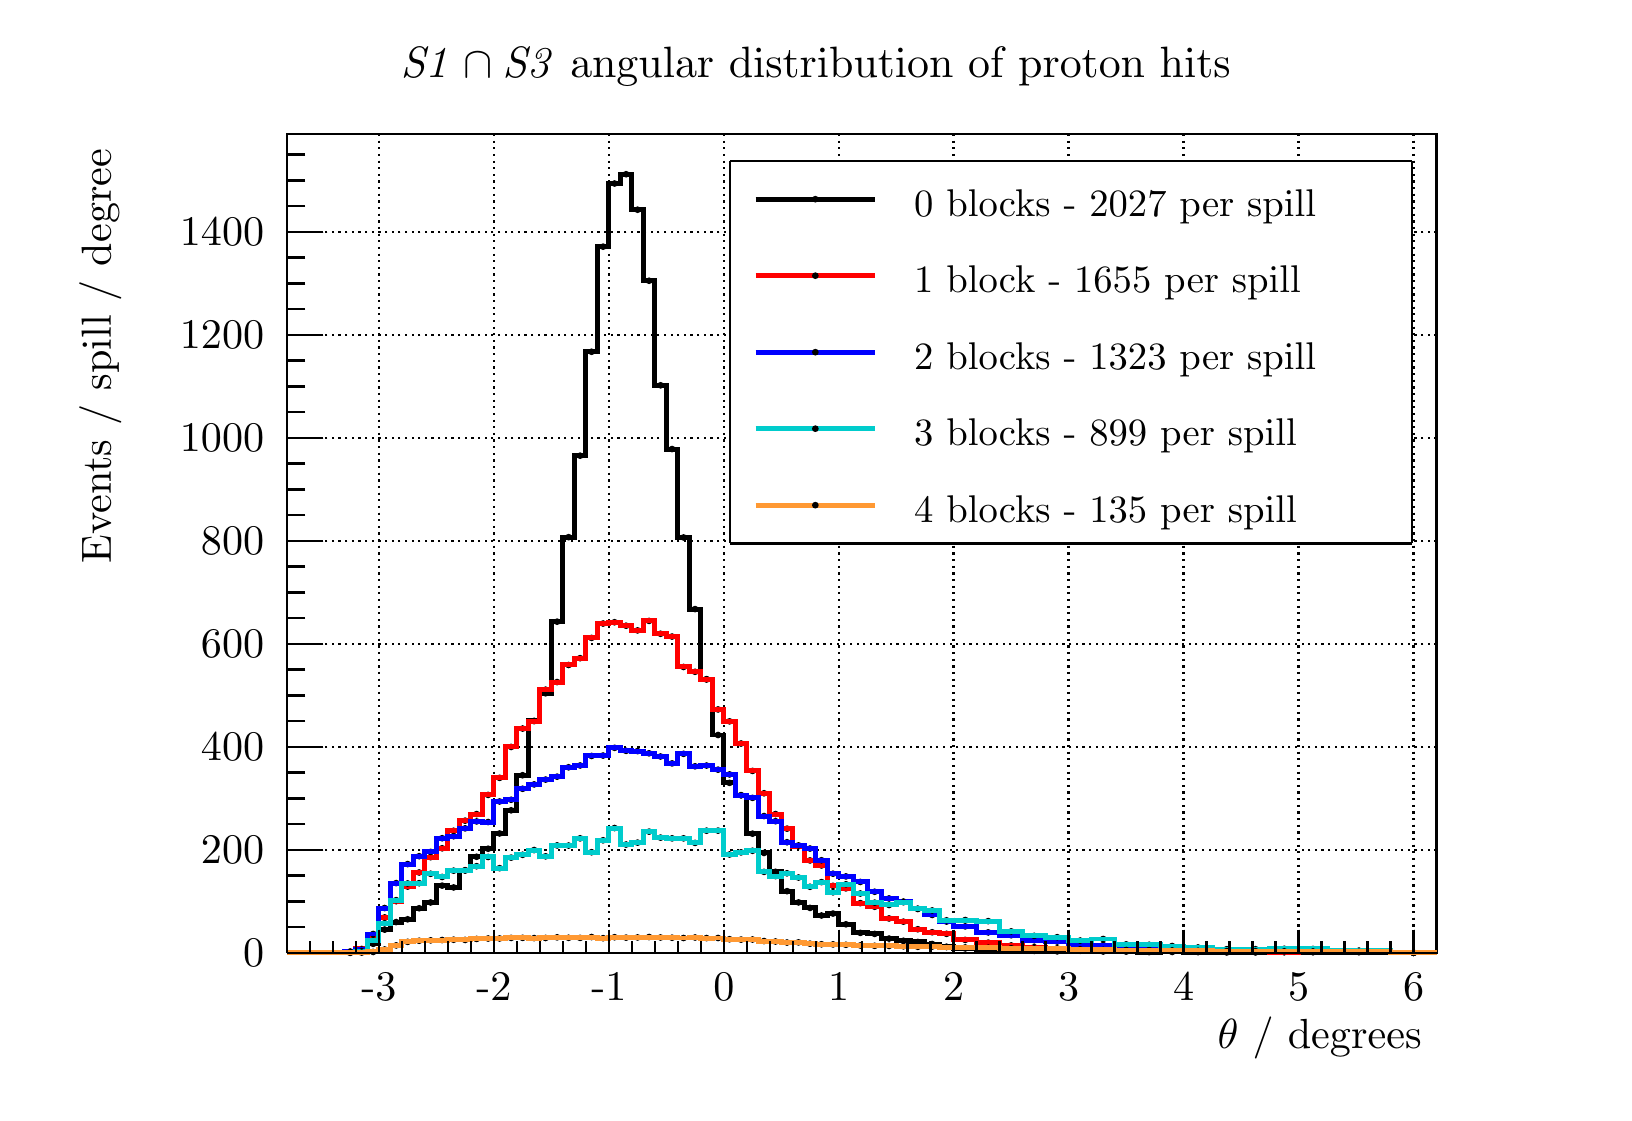
\begin{tikzpicture}
\pgfdeclareplotmark{cross} {
\pgfpathmoveto{\pgfpoint{-0.3\pgfplotmarksize}{\pgfplotmarksize}}
\pgfpathlineto{\pgfpoint{+0.3\pgfplotmarksize}{\pgfplotmarksize}}
\pgfpathlineto{\pgfpoint{+0.3\pgfplotmarksize}{0.3\pgfplotmarksize}}
\pgfpathlineto{\pgfpoint{+1\pgfplotmarksize}{0.3\pgfplotmarksize}}
\pgfpathlineto{\pgfpoint{+1\pgfplotmarksize}{-0.3\pgfplotmarksize}}
\pgfpathlineto{\pgfpoint{+0.3\pgfplotmarksize}{-0.3\pgfplotmarksize}}
\pgfpathlineto{\pgfpoint{+0.3\pgfplotmarksize}{-1.\pgfplotmarksize}}
\pgfpathlineto{\pgfpoint{-0.3\pgfplotmarksize}{-1.\pgfplotmarksize}}
\pgfpathlineto{\pgfpoint{-0.3\pgfplotmarksize}{-0.3\pgfplotmarksize}}
\pgfpathlineto{\pgfpoint{-1.\pgfplotmarksize}{-0.3\pgfplotmarksize}}
\pgfpathlineto{\pgfpoint{-1.\pgfplotmarksize}{0.3\pgfplotmarksize}}
\pgfpathlineto{\pgfpoint{-0.3\pgfplotmarksize}{0.3\pgfplotmarksize}}
\pgfpathclose
\pgfusepathqstroke
}
\pgfdeclareplotmark{cross*} {
\pgfpathmoveto{\pgfpoint{-0.3\pgfplotmarksize}{\pgfplotmarksize}}
\pgfpathlineto{\pgfpoint{+0.3\pgfplotmarksize}{\pgfplotmarksize}}
\pgfpathlineto{\pgfpoint{+0.3\pgfplotmarksize}{0.3\pgfplotmarksize}}
\pgfpathlineto{\pgfpoint{+1\pgfplotmarksize}{0.3\pgfplotmarksize}}
\pgfpathlineto{\pgfpoint{+1\pgfplotmarksize}{-0.3\pgfplotmarksize}}
\pgfpathlineto{\pgfpoint{+0.3\pgfplotmarksize}{-0.3\pgfplotmarksize}}
\pgfpathlineto{\pgfpoint{+0.3\pgfplotmarksize}{-1.\pgfplotmarksize}}
\pgfpathlineto{\pgfpoint{-0.3\pgfplotmarksize}{-1.\pgfplotmarksize}}
\pgfpathlineto{\pgfpoint{-0.3\pgfplotmarksize}{-0.3\pgfplotmarksize}}
\pgfpathlineto{\pgfpoint{-1.\pgfplotmarksize}{-0.3\pgfplotmarksize}}
\pgfpathlineto{\pgfpoint{-1.\pgfplotmarksize}{0.3\pgfplotmarksize}}
\pgfpathlineto{\pgfpoint{-0.3\pgfplotmarksize}{0.3\pgfplotmarksize}}
\pgfpathclose
\pgfusepathqfillstroke
}
\pgfdeclareplotmark{newstar} {
\pgfpathmoveto{\pgfqpoint{0pt}{\pgfplotmarksize}}
\pgfpathlineto{\pgfqpointpolar{44}{0.5\pgfplotmarksize}}
\pgfpathlineto{\pgfqpointpolar{18}{\pgfplotmarksize}}
\pgfpathlineto{\pgfqpointpolar{-20}{0.5\pgfplotmarksize}}
\pgfpathlineto{\pgfqpointpolar{-54}{\pgfplotmarksize}}
\pgfpathlineto{\pgfqpointpolar{-90}{0.5\pgfplotmarksize}}
\pgfpathlineto{\pgfqpointpolar{234}{\pgfplotmarksize}}
\pgfpathlineto{\pgfqpointpolar{198}{0.5\pgfplotmarksize}}
\pgfpathlineto{\pgfqpointpolar{162}{\pgfplotmarksize}}
\pgfpathlineto{\pgfqpointpolar{134}{0.5\pgfplotmarksize}}
\pgfpathclose
\pgfusepathqstroke
}
\pgfdeclareplotmark{newstar*} {
\pgfpathmoveto{\pgfqpoint{0pt}{\pgfplotmarksize}}
\pgfpathlineto{\pgfqpointpolar{44}{0.5\pgfplotmarksize}}
\pgfpathlineto{\pgfqpointpolar{18}{\pgfplotmarksize}}
\pgfpathlineto{\pgfqpointpolar{-20}{0.5\pgfplotmarksize}}
\pgfpathlineto{\pgfqpointpolar{-54}{\pgfplotmarksize}}
\pgfpathlineto{\pgfqpointpolar{-90}{0.5\pgfplotmarksize}}
\pgfpathlineto{\pgfqpointpolar{234}{\pgfplotmarksize}}
\pgfpathlineto{\pgfqpointpolar{198}{0.5\pgfplotmarksize}}
\pgfpathlineto{\pgfqpointpolar{162}{\pgfplotmarksize}}
\pgfpathlineto{\pgfqpointpolar{134}{0.5\pgfplotmarksize}}
\pgfpathclose
\pgfusepathqfillstroke
}
\definecolor{c}{rgb}{1,1,1};
\draw [color=c, fill=c] (0,0) rectangle (20,13.5143);
\draw [color=c, fill=c] (3.28571,1.77143) rectangle (17.8857,12.1714);
\definecolor{c}{rgb}{0,0,0};
\draw [c,line width=0.9] (3.28571,1.77143) -- (3.28571,12.1714) -- (17.8857,12.1714) -- (17.8857,1.77143) -- (3.28571,1.77143);
\definecolor{c}{rgb}{1,1,1};
\draw [color=c, fill=c] (3.28571,1.77143) rectangle (17.8857,12.1714);
\definecolor{c}{rgb}{0,0,0};
\draw [c,line width=0.9] (3.28571,1.77143) -- (3.28571,12.1714) -- (17.8857,12.1714) -- (17.8857,1.77143) -- (3.28571,1.77143);
\draw [c,line width=0.9] (3.28571,1.77143) -- (17.8857,1.77143);
\draw [c,dash pattern=on 0.80pt off 1.60pt ,line width=0.9] (4.45371,12.1714) -- (4.45371,1.77143);
\draw [c,dash pattern=on 0.80pt off 1.60pt ,line width=0.9] (5.91371,12.1714) -- (5.91371,1.77143);
\draw [c,dash pattern=on 0.80pt off 1.60pt ,line width=0.9] (7.37371,12.1714) -- (7.37371,1.77143);
\draw [c,dash pattern=on 0.80pt off 1.60pt ,line width=0.9] (8.83371,12.1714) -- (8.83371,1.77143);
\draw [c,dash pattern=on 0.80pt off 1.60pt ,line width=0.9] (10.2937,12.1714) -- (10.2937,1.77143);
\draw [c,dash pattern=on 0.80pt off 1.60pt ,line width=0.9] (11.7537,12.1714) -- (11.7537,1.77143);
\draw [c,dash pattern=on 0.80pt off 1.60pt ,line width=0.9] (13.2137,12.1714) -- (13.2137,1.77143);
\draw [c,dash pattern=on 0.80pt off 1.60pt ,line width=0.9] (14.6737,12.1714) -- (14.6737,1.77143);
\draw [c,dash pattern=on 0.80pt off 1.60pt ,line width=0.9] (16.1337,12.1714) -- (16.1337,1.77143);
\draw [c,dash pattern=on 0.80pt off 1.60pt ,line width=0.9] (17.5937,12.1714) -- (17.5937,1.77143);
\draw [c,dash pattern=on 0.80pt off 1.60pt ,line width=0.9] (4.45371,12.1714) -- (4.45371,1.77143);
\draw [c,dash pattern=on 0.80pt off 1.60pt ,line width=0.9] (17.5937,12.1714) -- (17.5937,1.77143);
\draw [c,line width=0.9] (3.28571,1.77143) -- (3.28571,12.1714);
\draw [c,dash pattern=on 0.80pt off 1.60pt ,line width=0.9] (17.8857,1.77143) -- (3.28571,1.77143);
\draw [c,dash pattern=on 0.80pt off 1.60pt ,line width=0.9] (17.8857,3.07955) -- (3.28571,3.07955);
\draw [c,dash pattern=on 0.80pt off 1.60pt ,line width=0.9] (17.8857,4.38766) -- (3.28571,4.38766);
\draw [c,dash pattern=on 0.80pt off 1.60pt ,line width=0.9] (17.8857,5.69578) -- (3.28571,5.69578);
\draw [c,dash pattern=on 0.80pt off 1.60pt ,line width=0.9] (17.8857,7.0039) -- (3.28571,7.0039);
\draw [c,dash pattern=on 0.80pt off 1.60pt ,line width=0.9] (17.8857,8.31201) -- (3.28571,8.31201);
\draw [c,dash pattern=on 0.80pt off 1.60pt ,line width=0.9] (17.8857,9.62013) -- (3.28571,9.62013);
\draw [c,dash pattern=on 0.80pt off 1.60pt ,line width=0.9] (17.8857,10.9282) -- (3.28571,10.9282);
\draw [c,dash pattern=on 0.80pt off 1.60pt ,line width=0.9] (17.8857,10.9282) -- (3.28571,10.9282);
\definecolor{c}{rgb}{0,0,0.6};
\draw [c,line width=0.9] (3.28571,1.77143) -- (3.43171,1.77143) -- (3.43171,1.77143) -- (3.57771,1.77143) -- (3.57771,1.77143) -- (3.72371,1.77143) -- (3.72371,1.77143) -- (3.86971,1.77143) -- (3.86971,1.77143) -- (4.01571,1.77143) --
 (4.01571,1.77143) -- (4.16171,1.77143) -- (4.16171,1.77143) -- (4.30771,1.77143) -- (4.30771,1.77143) -- (4.45371,1.77143) -- (4.45371,1.77143) -- (4.59971,1.77143) -- (4.59971,1.77143) -- (4.74571,1.77143) -- (4.74571,1.77143) -- (4.89171,1.77143)
 -- (4.89171,1.77143) -- (5.03771,1.77143) -- (5.03771,1.77143) -- (5.18371,1.77143) -- (5.18371,1.77143) -- (5.32971,1.77143) -- (5.32971,1.77143) -- (5.47571,1.77143) -- (5.47571,1.77143) -- (5.62171,1.77143) -- (5.62171,1.77143) --
 (5.76771,1.77143) -- (5.76771,1.77143) -- (5.91371,1.77143) -- (5.91371,1.77143) -- (6.05971,1.77143) -- (6.05971,1.77143) -- (6.20571,1.77143) -- (6.20571,1.77143) -- (6.35171,1.77143) -- (6.35171,1.77143) -- (6.49771,1.77143) -- (6.49771,1.77143)
 -- (6.64371,1.77143) -- (6.64371,1.77143) -- (6.78971,1.77143) -- (6.78971,1.77143) -- (6.93571,1.77143) -- (6.93571,1.77143) -- (7.08171,1.77143) -- (7.08171,1.77143) -- (7.22771,1.77143) -- (7.22771,1.77143) -- (7.37371,1.77143) --
 (7.37371,1.77143) -- (7.51971,1.77143) -- (7.51971,1.77143) -- (7.66571,1.77143) -- (7.66571,1.77143) -- (7.81171,1.77143) -- (7.81171,1.77143) -- (7.95771,1.77143) -- (7.95771,1.77143) -- (8.10371,1.77143) -- (8.10371,1.77143) -- (8.24971,1.77143)
 -- (8.24971,1.77143) -- (8.39571,1.77143) -- (8.39571,1.77143) -- (8.54171,1.77143) -- (8.54171,1.77143) -- (8.68771,1.77143) -- (8.68771,1.77143) -- (8.83371,1.77143) -- (8.83371,1.77143) -- (8.97971,1.77143) -- (8.97971,1.77143) --
 (9.12571,1.77143) -- (9.12571,1.77143) -- (9.27171,1.77143) -- (9.27171,1.77143) -- (9.41771,1.77143) -- (9.41771,1.77143) -- (9.56371,1.77143) -- (9.56371,1.77143) -- (9.70971,1.77143) -- (9.70971,1.77143) -- (9.85571,1.77143) -- (9.85571,1.77143)
 -- (10.0017,1.77143) -- (10.0017,1.77143) -- (10.1477,1.77143) -- (10.1477,1.77143) -- (10.2937,1.77143) -- (10.2937,1.77143) -- (10.4762,1.77143) -- (10.4762,1.77143) -- (10.6587,1.77143) -- (10.6587,1.77143) -- (10.8412,1.77143) --
 (10.8412,1.77143) -- (11.0237,1.77143) -- (11.0237,1.77143) -- (11.2062,1.77143) -- (11.2062,1.77143) -- (11.3887,1.77143) -- (11.3887,1.77143) -- (11.5712,1.77143) -- (11.5712,1.77143) -- (11.7537,1.77143) -- (11.7537,1.77143) -- (12.0457,1.77143)
 -- (12.0457,1.77143) -- (12.3377,1.77143) -- (12.3377,1.77143) -- (12.6297,1.77143) -- (12.6297,1.77143) -- (12.9217,1.77143) -- (12.9217,1.77143) -- (13.2137,1.77143) -- (13.2137,1.77143) -- (13.5057,1.77143) -- (13.5057,1.77143) --
 (13.7977,1.77143) -- (13.7977,1.77143) -- (14.0897,1.77143) -- (14.0897,1.77143) -- (14.3817,1.77143) -- (14.3817,1.77143) -- (14.6737,1.77143) -- (14.6737,1.77143) -- (15.0387,1.77143) -- (15.0387,1.77143) -- (15.4037,1.77143) -- (15.4037,1.77143)
 -- (15.7687,1.77143) -- (15.7687,1.77143) -- (16.1337,1.77143) -- (16.1337,1.77143) -- (16.4987,1.77143) -- (16.4987,1.77143) -- (17.3017,1.77143) -- (17.3017,1.77143) -- (17.8857,1.77143);
\definecolor{c}{rgb}{0,0,0};
\draw [c,line width=0.9] (3.28571,1.77143) -- (17.8857,1.77143);
\draw [c,line width=0.9] (4.45371,2.06739) -- (4.45371,1.77143);
\draw [c,line width=0.9] (4.74571,1.91941) -- (4.74571,1.77143);
\draw [c,line width=0.9] (5.03771,1.91941) -- (5.03771,1.77143);
\draw [c,line width=0.9] (5.32971,1.91941) -- (5.32971,1.77143);
\draw [c,line width=0.9] (5.62171,1.91941) -- (5.62171,1.77143);
\draw [c,line width=0.9] (5.91371,2.06739) -- (5.91371,1.77143);
\draw [c,line width=0.9] (6.20571,1.91941) -- (6.20571,1.77143);
\draw [c,line width=0.9] (6.49771,1.91941) -- (6.49771,1.77143);
\draw [c,line width=0.9] (6.78971,1.91941) -- (6.78971,1.77143);
\draw [c,line width=0.9] (7.08171,1.91941) -- (7.08171,1.77143);
\draw [c,line width=0.9] (7.37371,2.06739) -- (7.37371,1.77143);
\draw [c,line width=0.9] (7.66571,1.91941) -- (7.66571,1.77143);
\draw [c,line width=0.9] (7.95771,1.91941) -- (7.95771,1.77143);
\draw [c,line width=0.9] (8.24971,1.91941) -- (8.24971,1.77143);
\draw [c,line width=0.9] (8.54171,1.91941) -- (8.54171,1.77143);
\draw [c,line width=0.9] (8.83371,2.06739) -- (8.83371,1.77143);
\draw [c,line width=0.9] (9.12571,1.91941) -- (9.12571,1.77143);
\draw [c,line width=0.9] (9.41771,1.91941) -- (9.41771,1.77143);
\draw [c,line width=0.9] (9.70971,1.91941) -- (9.70971,1.77143);
\draw [c,line width=0.9] (10.0017,1.91941) -- (10.0017,1.77143);
\draw [c,line width=0.9] (10.2937,2.06739) -- (10.2937,1.77143);
\draw [c,line width=0.9] (10.5857,1.91941) -- (10.5857,1.77143);
\draw [c,line width=0.9] (10.8777,1.91941) -- (10.8777,1.77143);
\draw [c,line width=0.9] (11.1697,1.91941) -- (11.1697,1.77143);
\draw [c,line width=0.9] (11.4617,1.91941) -- (11.4617,1.77143);
\draw [c,line width=0.9] (11.7537,2.06739) -- (11.7537,1.77143);
\draw [c,line width=0.9] (12.0457,1.91941) -- (12.0457,1.77143);
\draw [c,line width=0.9] (12.3377,1.91941) -- (12.3377,1.77143);
\draw [c,line width=0.9] (12.6297,1.91941) -- (12.6297,1.77143);
\draw [c,line width=0.9] (12.9217,1.91941) -- (12.9217,1.77143);
\draw [c,line width=0.9] (13.2137,2.06739) -- (13.2137,1.77143);
\draw [c,line width=0.9] (13.5057,1.91941) -- (13.5057,1.77143);
\draw [c,line width=0.9] (13.7977,1.91941) -- (13.7977,1.77143);
\draw [c,line width=0.9] (14.0897,1.91941) -- (14.0897,1.77143);
\draw [c,line width=0.9] (14.3817,1.91941) -- (14.3817,1.77143);
\draw [c,line width=0.9] (14.6737,2.06739) -- (14.6737,1.77143);
\draw [c,line width=0.9] (14.9657,1.91941) -- (14.9657,1.77143);
\draw [c,line width=0.9] (15.2577,1.91941) -- (15.2577,1.77143);
\draw [c,line width=0.9] (15.5497,1.91941) -- (15.5497,1.77143);
\draw [c,line width=0.9] (15.8417,1.91941) -- (15.8417,1.77143);
\draw [c,line width=0.9] (16.1337,2.06739) -- (16.1337,1.77143);
\draw [c,line width=0.9] (16.4257,1.91941) -- (16.4257,1.77143);
\draw [c,line width=0.9] (16.7177,1.91941) -- (16.7177,1.77143);
\draw [c,line width=0.9] (17.0097,1.91941) -- (17.0097,1.77143);
\draw [c,line width=0.9] (17.3017,1.91941) -- (17.3017,1.77143);
\draw [c,line width=0.9] (17.5937,2.06739) -- (17.5937,1.77143);
\draw [c,line width=0.9] (4.45371,2.06739) -- (4.45371,1.77143);
\draw [c,line width=0.9] (4.16171,1.91941) -- (4.16171,1.77143);
\draw [c,line width=0.9] (3.86971,1.91941) -- (3.86971,1.77143);
\draw [c,line width=0.9] (3.57771,1.91941) -- (3.57771,1.77143);
\draw [c,line width=0.9] (17.5937,2.06739) -- (17.5937,1.77143);
\draw [anchor=base] (4.45371,1.16329) node[scale=1.52295, color=c, rotate=0]{-3};
\draw [anchor=base] (5.91371,1.16329) node[scale=1.52295, color=c, rotate=0]{-2};
\draw [anchor=base] (7.37371,1.16329) node[scale=1.52295, color=c, rotate=0]{-1};
\draw [anchor=base] (8.83371,1.16329) node[scale=1.52295, color=c, rotate=0]{0};
\draw [anchor=base] (10.2937,1.16329) node[scale=1.52295, color=c, rotate=0]{1};
\draw [anchor=base] (11.7537,1.16329) node[scale=1.52295, color=c, rotate=0]{2};
\draw [anchor=base] (13.2137,1.16329) node[scale=1.52295, color=c, rotate=0]{3};
\draw [anchor=base] (14.6737,1.16329) node[scale=1.52295, color=c, rotate=0]{4};
\draw [anchor=base] (16.1337,1.16329) node[scale=1.52295, color=c, rotate=0]{5};
\draw [anchor=base] (17.5937,1.16329) node[scale=1.52295, color=c, rotate=0]{6};
\draw [anchor= east] (17.8857,0.690286) node[scale=1.52295, color=c, rotate=0]{$\theta$ / degrees};
\draw [c,line width=0.9] (3.28571,1.77143) -- (3.28571,12.1714);
\draw [c,line width=0.9] (3.74745,1.77143) -- (3.28571,1.77143);
\draw [c,line width=0.9] (3.51658,2.09846) -- (3.28571,2.09846);
\draw [c,line width=0.9] (3.51658,2.42549) -- (3.28571,2.42549);
\draw [c,line width=0.9] (3.51658,2.75252) -- (3.28571,2.75252);
\draw [c,line width=0.9] (3.74745,3.07955) -- (3.28571,3.07955);
\draw [c,line width=0.9] (3.51658,3.40658) -- (3.28571,3.40658);
\draw [c,line width=0.9] (3.51658,3.7336) -- (3.28571,3.7336);
\draw [c,line width=0.9] (3.51658,4.06063) -- (3.28571,4.06063);
\draw [c,line width=0.9] (3.74745,4.38766) -- (3.28571,4.38766);
\draw [c,line width=0.9] (3.51658,4.71469) -- (3.28571,4.71469);
\draw [c,line width=0.9] (3.51658,5.04172) -- (3.28571,5.04172);
\draw [c,line width=0.9] (3.51658,5.36875) -- (3.28571,5.36875);
\draw [c,line width=0.9] (3.74745,5.69578) -- (3.28571,5.69578);
\draw [c,line width=0.9] (3.51658,6.02281) -- (3.28571,6.02281);
\draw [c,line width=0.9] (3.51658,6.34984) -- (3.28571,6.34984);
\draw [c,line width=0.9] (3.51658,6.67687) -- (3.28571,6.67687);
\draw [c,line width=0.9] (3.74745,7.0039) -- (3.28571,7.0039);
\draw [c,line width=0.9] (3.51658,7.33093) -- (3.28571,7.33093);
\draw [c,line width=0.9] (3.51658,7.65796) -- (3.28571,7.65796);
\draw [c,line width=0.9] (3.51658,7.98499) -- (3.28571,7.98499);
\draw [c,line width=0.9] (3.74745,8.31201) -- (3.28571,8.31201);
\draw [c,line width=0.9] (3.51658,8.63904) -- (3.28571,8.63904);
\draw [c,line width=0.9] (3.51658,8.96607) -- (3.28571,8.96607);
\draw [c,line width=0.9] (3.51658,9.2931) -- (3.28571,9.2931);
\draw [c,line width=0.9] (3.74745,9.62013) -- (3.28571,9.62013);
\draw [c,line width=0.9] (3.51658,9.94716) -- (3.28571,9.94716);
\draw [c,line width=0.9] (3.51658,10.2742) -- (3.28571,10.2742);
\draw [c,line width=0.9] (3.51658,10.6012) -- (3.28571,10.6012);
\draw [c,line width=0.9] (3.74745,10.9282) -- (3.28571,10.9282);
\draw [c,line width=0.9] (3.74745,10.9282) -- (3.28571,10.9282);
\draw [c,line width=0.9] (3.51658,11.2553) -- (3.28571,11.2553);
\draw [c,line width=0.9] (3.51658,11.5823) -- (3.28571,11.5823);
\draw [c,line width=0.9] (3.51658,11.9093) -- (3.28571,11.9093);
\draw [anchor= east] (3.18571,1.77143) node[scale=1.52295, color=c, rotate=0]{0};
\draw [anchor= east] (3.18571,3.07955) node[scale=1.52295, color=c, rotate=0]{200};
\draw [anchor= east] (3.18571,4.38766) node[scale=1.52295, color=c, rotate=0]{400};
\draw [anchor= east] (3.18571,5.69578) node[scale=1.52295, color=c, rotate=0]{600};
\draw [anchor= east] (3.18571,7.0039) node[scale=1.52295, color=c, rotate=0]{800};
\draw [anchor= east] (3.18571,8.31201) node[scale=1.52295, color=c, rotate=0]{1000};
\draw [anchor= east] (3.18571,9.62013) node[scale=1.52295, color=c, rotate=0]{1200};
\draw [anchor= east] (3.18571,10.9282) node[scale=1.52295, color=c, rotate=0]{1400};
\draw [anchor= east] (0.914286,12.1714) node[scale=1.52295, color=c, rotate=90]{ Events / spill / degree};
\draw [c,line width=1.8] (4.08871,1.77928) -- (4.08871,1.77976);
\draw [c,line width=1.8] (4.08871,1.77976) -- (4.08871,1.78025);
\foreach \P in {(4.08871,1.77976)}{\draw[mark options={color=c,fill=c},mark size=2.402402pt,mark=*,mark size=1pt] plot coordinates {\P};}
\draw [c,line width=1.8] (4.23471,1.80702) -- (4.23471,1.808);
\draw [c,line width=1.8] (4.23471,1.808) -- (4.23471,1.80898);
\foreach \P in {(4.23471,1.808)}{\draw[mark options={color=c,fill=c},mark size=2.402402pt,mark=*,mark size=1pt] plot coordinates {\P};}
\draw [c,line width=1.8] (4.38071,1.88391) -- (4.38071,1.88565);
\draw [c,line width=1.8] (4.38071,1.88565) -- (4.38071,1.88738);
\foreach \P in {(4.38071,1.88565)}{\draw[mark options={color=c,fill=c},mark size=2.402402pt,mark=*,mark size=1pt] plot coordinates {\P};}
\draw [c,line width=1.8] (4.52671,2.0637) -- (4.52671,2.0665);
\draw [c,line width=1.8] (4.52671,2.0665) -- (4.52671,2.0693);
\foreach \P in {(4.52671,2.0665)}{\draw[mark options={color=c,fill=c},mark size=2.402402pt,mark=*,mark size=1pt] plot coordinates {\P};}
\draw [c,line width=1.8] (4.67271,2.15927) -- (4.67271,2.16245);
\draw [c,line width=1.8] (4.67271,2.16245) -- (4.67271,2.16564);
\foreach \P in {(4.67271,2.16245)}{\draw[mark options={color=c,fill=c},mark size=2.402402pt,mark=*,mark size=1pt] plot coordinates {\P};}
\draw [c,line width=1.8] (4.81871,2.19429) -- (4.81871,2.19763);
\draw [c,line width=1.8] (4.81871,2.19763) -- (4.81871,2.20096);
\foreach \P in {(4.81871,2.19763)}{\draw[mark options={color=c,fill=c},mark size=2.402402pt,mark=*,mark size=1pt] plot coordinates {\P};}
\draw [c,line width=1.8] (4.96471,2.33421) -- (4.96471,2.33808);
\draw [c,line width=1.8] (4.96471,2.33808) -- (4.96471,2.34194);
\foreach \P in {(4.96471,2.33808)}{\draw[mark options={color=c,fill=c},mark size=2.402402pt,mark=*,mark size=1pt] plot coordinates {\P};}
\draw [c,line width=1.8] (5.11071,2.40725) -- (5.11071,2.41137);
\draw [c,line width=1.8] (5.11071,2.41137) -- (5.11071,2.41549);
\foreach \P in {(5.11071,2.41137)}{\draw[mark options={color=c,fill=c},mark size=2.402402pt,mark=*,mark size=1pt] plot coordinates {\P};}
\draw [c,line width=1.8] (5.25671,2.62065) -- (5.25671,2.62539);
\draw [c,line width=1.8] (5.25671,2.62539) -- (5.25671,2.63013);
\foreach \P in {(5.25671,2.62539)}{\draw[mark options={color=c,fill=c},mark size=2.402402pt,mark=*,mark size=1pt] plot coordinates {\P};}
\draw [c,line width=1.8] (5.40271,2.5977) -- (5.40271,2.60239);
\draw [c,line width=1.8] (5.40271,2.60239) -- (5.40271,2.60707);
\foreach \P in {(5.40271,2.60239)}{\draw[mark options={color=c,fill=c},mark size=2.402402pt,mark=*,mark size=1pt] plot coordinates {\P};}
\draw [c,line width=1.8] (5.54871,2.8114) -- (5.54871,2.81666);
\draw [c,line width=1.8] (5.54871,2.81666) -- (5.54871,2.82192);
\foreach \P in {(5.54871,2.81666)}{\draw[mark options={color=c,fill=c},mark size=2.402402pt,mark=*,mark size=1pt] plot coordinates {\P};}
\draw [c,line width=1.8] (5.69471,2.9861) -- (5.69471,2.99178);
\draw [c,line width=1.8] (5.69471,2.99178) -- (5.69471,2.99746);
\foreach \P in {(5.69471,2.99178)}{\draw[mark options={color=c,fill=c},mark size=2.402402pt,mark=*,mark size=1pt] plot coordinates {\P};}
\draw [c,line width=1.8] (5.84071,3.08772) -- (5.84071,3.09363);
\draw [c,line width=1.8] (5.84071,3.09363) -- (5.84071,3.09954);
\foreach \P in {(5.84071,3.09363)}{\draw[mark options={color=c,fill=c},mark size=2.402402pt,mark=*,mark size=1pt] plot coordinates {\P};}
\draw [c,line width=1.8] (5.98671,3.28119) -- (5.98671,3.28753);
\draw [c,line width=1.8] (5.98671,3.28753) -- (5.98671,3.29387);
\foreach \P in {(5.98671,3.28753)}{\draw[mark options={color=c,fill=c},mark size=2.402402pt,mark=*,mark size=1pt] plot coordinates {\P};}
\draw [c,line width=1.8] (6.13271,3.57494) -- (6.13271,3.58187);
\draw [c,line width=1.8] (6.13271,3.58187) -- (6.13271,3.58879);
\foreach \P in {(6.13271,3.58187)}{\draw[mark options={color=c,fill=c},mark size=2.402402pt,mark=*,mark size=1pt] plot coordinates {\P};}
\draw [c,line width=1.8] (6.27871,4.01937) -- (6.27871,4.02712);
\draw [c,line width=1.8] (6.27871,4.02712) -- (6.27871,4.03486);
\foreach \P in {(6.27871,4.02712)}{\draw[mark options={color=c,fill=c},mark size=2.402402pt,mark=*,mark size=1pt] plot coordinates {\P};}
\draw [c,line width=1.8] (6.42471,4.70892) -- (6.42471,4.71772);
\draw [c,line width=1.8] (6.42471,4.71772) -- (6.42471,4.72652);
\foreach \P in {(6.42471,4.71772)}{\draw[mark options={color=c,fill=c},mark size=2.402402pt,mark=*,mark size=1pt] plot coordinates {\P};}
\draw [c,line width=1.8] (6.57071,5.05873) -- (6.57071,5.06808);
\draw [c,line width=1.8] (6.57071,5.06808) -- (6.57071,5.07743);
\foreach \P in {(6.57071,5.06808)}{\draw[mark options={color=c,fill=c},mark size=2.402402pt,mark=*,mark size=1pt] plot coordinates {\P};}
\draw [c,line width=1.8] (6.71671,5.96677) -- (6.71671,5.9773);
\draw [c,line width=1.8] (6.71671,5.9773) -- (6.71671,5.98784);
\foreach \P in {(6.71671,5.9773)}{\draw[mark options={color=c,fill=c},mark size=2.402402pt,mark=*,mark size=1pt] plot coordinates {\P};}
\draw [c,line width=1.8] (6.86271,7.03879) -- (6.86271,7.05058);
\draw [c,line width=1.8] (6.86271,7.05058) -- (6.86271,7.06238);
\foreach \P in {(6.86271,7.05058)}{\draw[mark options={color=c,fill=c},mark size=2.402402pt,mark=*,mark size=1pt] plot coordinates {\P};}
\draw [c,line width=1.8] (7.00871,8.07255) -- (7.00871,8.08548);
\draw [c,line width=1.8] (7.00871,8.08548) -- (7.00871,8.09841);
\foreach \P in {(7.00871,8.08548)}{\draw[mark options={color=c,fill=c},mark size=2.402402pt,mark=*,mark size=1pt] plot coordinates {\P};}
\draw [c,line width=1.8] (7.15471,9.39111) -- (7.15471,9.40531);
\draw [c,line width=1.8] (7.15471,9.40531) -- (7.15471,9.41952);
\foreach \P in {(7.15471,9.40531)}{\draw[mark options={color=c,fill=c},mark size=2.402402pt,mark=*,mark size=1pt] plot coordinates {\P};}
\draw [c,line width=1.8] (7.30071,10.7244) -- (7.30071,10.7398);
\draw [c,line width=1.8] (7.30071,10.7398) -- (7.30071,10.7552);
\foreach \P in {(7.30071,10.7398)}{\draw[mark options={color=c,fill=c},mark size=2.402402pt,mark=*,mark size=1pt] plot coordinates {\P};}
\draw [c,line width=1.8] (7.44671,11.5259) -- (7.44671,11.542);
\draw [c,line width=1.8] (7.44671,11.542) -- (7.44671,11.5581);
\foreach \P in {(7.44671,11.542)}{\draw[mark options={color=c,fill=c},mark size=2.402402pt,mark=*,mark size=1pt] plot coordinates {\P};}
\draw [c,line width=1.8] (7.59271,11.6439) -- (7.59271,11.66);
\draw [c,line width=1.8] (7.59271,11.66) -- (7.59271,11.6762);
\foreach \P in {(7.59271,11.66)}{\draw[mark options={color=c,fill=c},mark size=2.402402pt,mark=*,mark size=1pt] plot coordinates {\P};}
\draw [c,line width=1.8] (7.73871,11.1933) -- (7.73871,11.2091);
\draw [c,line width=1.8] (7.73871,11.2091) -- (7.73871,11.2249);
\foreach \P in {(7.73871,11.2091)}{\draw[mark options={color=c,fill=c},mark size=2.402402pt,mark=*,mark size=1pt] plot coordinates {\P};}
\draw [c,line width=1.8] (7.88471,10.292) -- (7.88471,10.307);
\draw [c,line width=1.8] (7.88471,10.307) -- (7.88471,10.322);
\foreach \P in {(7.88471,10.307)}{\draw[mark options={color=c,fill=c},mark size=2.402402pt,mark=*,mark size=1pt] plot coordinates {\P};}
\draw [c,line width=1.8] (8.03071,8.96539) -- (8.03071,8.97916);
\draw [c,line width=1.8] (8.03071,8.97916) -- (8.03071,8.99293);
\foreach \P in {(8.03071,8.97916)}{\draw[mark options={color=c,fill=c},mark size=2.402402pt,mark=*,mark size=1pt] plot coordinates {\P};}
\draw [c,line width=1.8] (8.17671,8.15671) -- (8.17671,8.1697);
\draw [c,line width=1.8] (8.17671,8.1697) -- (8.17671,8.18269);
\foreach \P in {(8.17671,8.1697)}{\draw[mark options={color=c,fill=c},mark size=2.402402pt,mark=*,mark size=1pt] plot coordinates {\P};}
\draw [c,line width=1.8] (8.32271,7.03519) -- (8.32271,7.04698);
\draw [c,line width=1.8] (8.32271,7.04698) -- (8.32271,7.05876);
\foreach \P in {(8.32271,7.04698)}{\draw[mark options={color=c,fill=c},mark size=2.402402pt,mark=*,mark size=1pt] plot coordinates {\P};}
\draw [c,line width=1.8] (8.46871,6.12634) -- (8.46871,6.13709);
\draw [c,line width=1.8] (8.46871,6.13709) -- (8.46871,6.14784);
\foreach \P in {(8.46871,6.13709)}{\draw[mark options={color=c,fill=c},mark size=2.402402pt,mark=*,mark size=1pt] plot coordinates {\P};}
\draw [c,line width=1.8] (8.61471,5.23363) -- (8.61471,5.24318);
\draw [c,line width=1.8] (8.61471,5.24318) -- (8.61471,5.25272);
\foreach \P in {(8.61471,5.24318)}{\draw[mark options={color=c,fill=c},mark size=2.402402pt,mark=*,mark size=1pt] plot coordinates {\P};}
\draw [c,line width=1.8] (8.76071,4.52978) -- (8.76071,4.53832);
\draw [c,line width=1.8] (8.76071,4.53832) -- (8.76071,4.54686);
\foreach \P in {(8.76071,4.53832)}{\draw[mark options={color=c,fill=c},mark size=2.402402pt,mark=*,mark size=1pt] plot coordinates {\P};}
\draw [c,line width=1.8] (8.90671,3.9228) -- (8.90671,3.93034);
\draw [c,line width=1.8] (8.90671,3.93034) -- (8.90671,3.93787);
\foreach \P in {(8.90671,3.93034)}{\draw[mark options={color=c,fill=c},mark size=2.402402pt,mark=*,mark size=1pt] plot coordinates {\P};}
\draw [c,line width=1.8] (9.05271,3.76622) -- (9.05271,3.77346);
\draw [c,line width=1.8] (9.05271,3.77346) -- (9.05271,3.7807);
\foreach \P in {(9.05271,3.77346)}{\draw[mark options={color=c,fill=c},mark size=2.402402pt,mark=*,mark size=1pt] plot coordinates {\P};}
\draw [c,line width=1.8] (9.19871,3.27871) -- (9.19871,3.28503);
\draw [c,line width=1.8] (9.19871,3.28503) -- (9.19871,3.29134);
\foreach \P in {(9.19871,3.28503)}{\draw[mark options={color=c,fill=c},mark size=2.402402pt,mark=*,mark size=1pt] plot coordinates {\P};}
\draw [c,line width=1.8] (9.34471,3.0343) -- (9.34471,3.0401);
\draw [c,line width=1.8] (9.34471,3.0401) -- (9.34471,3.04591);
\foreach \P in {(9.34471,3.0401)}{\draw[mark options={color=c,fill=c},mark size=2.402402pt,mark=*,mark size=1pt] plot coordinates {\P};}
\draw [c,line width=1.8] (9.49071,2.7953) -- (9.49071,2.8005);
\draw [c,line width=1.8] (9.49071,2.8005) -- (9.49071,2.8057);
\foreach \P in {(9.49071,2.8005)}{\draw[mark options={color=c,fill=c},mark size=2.402402pt,mark=*,mark size=1pt] plot coordinates {\P};}
\draw [c,line width=1.8] (9.63671,2.55056) -- (9.63671,2.55512);
\draw [c,line width=1.8] (9.63671,2.55512) -- (9.63671,2.55967);
\foreach \P in {(9.63671,2.55512)}{\draw[mark options={color=c,fill=c},mark size=2.402402pt,mark=*,mark size=1pt] plot coordinates {\P};}
\draw [c,line width=1.8] (9.78271,2.40811) -- (9.78271,2.41224);
\draw [c,line width=1.8] (9.78271,2.41224) -- (9.78271,2.41636);
\foreach \P in {(9.78271,2.41224)}{\draw[mark options={color=c,fill=c},mark size=2.402402pt,mark=*,mark size=1pt] plot coordinates {\P};}
\draw [c,line width=1.8] (9.92871,2.33856) -- (9.92871,2.34245);
\draw [c,line width=1.8] (9.92871,2.34245) -- (9.92871,2.34633);
\foreach \P in {(9.92871,2.34245)}{\draw[mark options={color=c,fill=c},mark size=2.402402pt,mark=*,mark size=1pt] plot coordinates {\P};}
\draw [c,line width=1.8] (10.0747,2.24253) -- (10.0747,2.24605);
\draw [c,line width=1.8] (10.0747,2.24605) -- (10.0747,2.24957);
\foreach \P in {(10.0747,2.24605)}{\draw[mark options={color=c,fill=c},mark size=2.402402pt,mark=*,mark size=1pt] plot coordinates {\P};}
\draw [c,line width=1.8] (10.2207,2.26683) -- (10.2207,2.27048);
\draw [c,line width=1.8] (10.2207,2.27048) -- (10.2207,2.27413);
\foreach \P in {(10.2207,2.27048)}{\draw[mark options={color=c,fill=c},mark size=2.402402pt,mark=*,mark size=1pt] plot coordinates {\P};}
\draw [c,line width=1.8] (10.385,2.13071) -- (10.385,2.13417);
\draw [c,line width=1.8] (10.385,2.13417) -- (10.385,2.13762);
\foreach \P in {(10.385,2.13417)}{\draw[mark options={color=c,fill=c},mark size=2.402402pt,mark=*,mark size=1pt] plot coordinates {\P};}
\draw [c,line width=1.8] (10.5675,2.0223) -- (10.5675,2.02518);
\draw [c,line width=1.8] (10.5675,2.02518) -- (10.5675,2.02807);
\foreach \P in {(10.5675,2.02518)}{\draw[mark options={color=c,fill=c},mark size=2.402402pt,mark=*,mark size=1pt] plot coordinates {\P};}
\draw [c,line width=1.8] (10.75,2.0093) -- (10.75,2.01214);
\draw [c,line width=1.8] (10.75,2.01214) -- (10.75,2.01497);
\foreach \P in {(10.75,2.01214)}{\draw[mark options={color=c,fill=c},mark size=2.402402pt,mark=*,mark size=1pt] plot coordinates {\P};}
\draw [c,line width=1.8] (10.9325,1.95041) -- (10.9325,1.95285);
\draw [c,line width=1.8] (10.9325,1.95285) -- (10.9325,1.95529);
\foreach \P in {(10.9325,1.95285)}{\draw[mark options={color=c,fill=c},mark size=2.402402pt,mark=*,mark size=1pt] plot coordinates {\P};}
\draw [c,line width=1.8] (11.115,1.92247) -- (11.115,1.92473);
\draw [c,line width=1.8] (11.115,1.92473) -- (11.115,1.92699);
\foreach \P in {(11.115,1.92473)}{\draw[mark options={color=c,fill=c},mark size=2.402402pt,mark=*,mark size=1pt] plot coordinates {\P};}
\draw [c,line width=1.8] (11.2975,1.90792) -- (11.2975,1.91006);
\draw [c,line width=1.8] (11.2975,1.91006) -- (11.2975,1.9122);
\foreach \P in {(11.2975,1.91006)}{\draw[mark options={color=c,fill=c},mark size=2.402402pt,mark=*,mark size=1pt] plot coordinates {\P};}
\draw [c,line width=1.8] (11.48,1.88169) -- (11.48,1.88362);
\draw [c,line width=1.8] (11.48,1.88362) -- (11.48,1.88556);
\foreach \P in {(11.48,1.88362)}{\draw[mark options={color=c,fill=c},mark size=2.402402pt,mark=*,mark size=1pt] plot coordinates {\P};}
\draw [c,line width=1.8] (11.6625,1.84719) -- (11.6625,1.84877);
\draw [c,line width=1.8] (11.6625,1.84877) -- (11.6625,1.85034);
\foreach \P in {(11.6625,1.84877)}{\draw[mark options={color=c,fill=c},mark size=2.402402pt,mark=*,mark size=1pt] plot coordinates {\P};}
\draw [c,line width=1.8] (11.8997,1.8255) -- (11.8997,1.82722);
\draw [c,line width=1.8] (11.8997,1.82722) -- (11.8997,1.82893);
\foreach \P in {(11.8997,1.82722)}{\draw[mark options={color=c,fill=c},mark size=2.402402pt,mark=*,mark size=1pt] plot coordinates {\P};}
\draw [c,line width=1.8] (12.1917,1.80911) -- (12.1917,1.81054);
\draw [c,line width=1.8] (12.1917,1.81054) -- (12.1917,1.81198);
\foreach \P in {(12.1917,1.81054)}{\draw[mark options={color=c,fill=c},mark size=2.402402pt,mark=*,mark size=1pt] plot coordinates {\P};}
\draw [c,line width=1.8] (12.4837,1.80809) -- (12.4837,1.80951);
\draw [c,line width=1.8] (12.4837,1.80951) -- (12.4837,1.81093);
\foreach \P in {(12.4837,1.80951)}{\draw[mark options={color=c,fill=c},mark size=2.402402pt,mark=*,mark size=1pt] plot coordinates {\P};}
\draw [c,line width=1.8] (12.7757,1.79522) -- (12.7757,1.79637);
\draw [c,line width=1.8] (12.7757,1.79637) -- (12.7757,1.79753);
\foreach \P in {(12.7757,1.79637)}{\draw[mark options={color=c,fill=c},mark size=2.402402pt,mark=*,mark size=1pt] plot coordinates {\P};}
\draw [c,line width=1.8] (13.0677,1.78926) -- (13.0677,1.79027);
\draw [c,line width=1.8] (13.0677,1.79027) -- (13.0677,1.79128);
\foreach \P in {(13.0677,1.79027)}{\draw[mark options={color=c,fill=c},mark size=2.402402pt,mark=*,mark size=1pt] plot coordinates {\P};}
\draw [c,line width=1.8] (13.3597,1.7964) -- (13.3597,1.79758);
\draw [c,line width=1.8] (13.3597,1.79758) -- (13.3597,1.79876);
\foreach \P in {(13.3597,1.79758)}{\draw[mark options={color=c,fill=c},mark size=2.402402pt,mark=*,mark size=1pt] plot coordinates {\P};}
\draw [c,line width=1.8] (13.6517,1.78712) -- (13.6517,1.78804);
\draw [c,line width=1.8] (13.6517,1.78804) -- (13.6517,1.78897);
\foreach \P in {(13.6517,1.78804)}{\draw[mark options={color=c,fill=c},mark size=2.402402pt,mark=*,mark size=1pt] plot coordinates {\P};}
\draw [c,line width=1.8] (13.9437,1.78641) -- (13.9437,1.78733);
\draw [c,line width=1.8] (13.9437,1.78733) -- (13.9437,1.78826);
\foreach \P in {(13.9437,1.78733)}{\draw[mark options={color=c,fill=c},mark size=2.402402pt,mark=*,mark size=1pt] plot coordinates {\P};}
\draw [c,line width=1.8] (14.2357,1.78046) -- (14.2357,1.7812);
\draw [c,line width=1.8] (14.2357,1.7812) -- (14.2357,1.78194);
\foreach \P in {(14.2357,1.7812)}{\draw[mark options={color=c,fill=c},mark size=2.402402pt,mark=*,mark size=1pt] plot coordinates {\P};}
\draw [c,line width=1.8] (14.5277,1.78232) -- (14.5277,1.7831);
\draw [c,line width=1.8] (14.5277,1.7831) -- (14.5277,1.78389);
\foreach \P in {(14.5277,1.7831)}{\draw[mark options={color=c,fill=c},mark size=2.402402pt,mark=*,mark size=1pt] plot coordinates {\P};}
\draw [c,line width=1.8] (14.8562,1.77979) -- (14.8562,1.78055);
\draw [c,line width=1.8] (14.8562,1.78055) -- (14.8562,1.78132);
\foreach \P in {(14.8562,1.78055)}{\draw[mark options={color=c,fill=c},mark size=2.402402pt,mark=*,mark size=1pt] plot coordinates {\P};}
\draw [c,line width=1.8] (15.2212,1.77593) -- (15.2212,1.7765);
\draw [c,line width=1.8] (15.2212,1.7765) -- (15.2212,1.77707);
\foreach \P in {(15.2212,1.7765)}{\draw[mark options={color=c,fill=c},mark size=2.402402pt,mark=*,mark size=1pt] plot coordinates {\P};}
\draw [c,line width=1.8] (15.5862,1.77596) -- (15.5862,1.77653);
\draw [c,line width=1.8] (15.5862,1.77653) -- (15.5862,1.7771);
\foreach \P in {(15.5862,1.77653)}{\draw[mark options={color=c,fill=c},mark size=2.402402pt,mark=*,mark size=1pt] plot coordinates {\P};}
\draw [c,line width=1.8] (15.9512,1.77912) -- (15.9512,1.77987);
\draw [c,line width=1.8] (15.9512,1.77987) -- (15.9512,1.78062);
\foreach \P in {(15.9512,1.77987)}{\draw[mark options={color=c,fill=c},mark size=2.402402pt,mark=*,mark size=1pt] plot coordinates {\P};}
\draw [c,line width=1.8] (16.3162,1.77848) -- (16.3162,1.77922);
\draw [c,line width=1.8] (16.3162,1.77922) -- (16.3162,1.77995);
\foreach \P in {(16.3162,1.77922)}{\draw[mark options={color=c,fill=c},mark size=2.402402pt,mark=*,mark size=1pt] plot coordinates {\P};}
\draw [c,line width=1.8] (16.9002,1.77875) -- (16.9002,1.77985);
\draw [c,line width=1.8] (16.9002,1.77985) -- (16.9002,1.78094);
\foreach \P in {(16.9002,1.77985)}{\draw[mark options={color=c,fill=c},mark size=2.402402pt,mark=*,mark size=1pt] plot coordinates {\P};}
\draw [c,line width=1.8] (17.5937,1.77212) -- (17.5937,1.77269);
\draw [c,line width=1.8] (17.5937,1.77269) -- (17.5937,1.77325);
\foreach \P in {(17.5937,1.77269)}{\draw[mark options={color=c,fill=c},mark size=2.402402pt,mark=*,mark size=1pt] plot coordinates {\P};}
\draw [c,line width=1.8] (3.28571,1.77143) -- (3.43171,1.77143) -- (3.43171,1.77143) -- (3.57771,1.77143) -- (3.57771,1.77143) -- (3.72371,1.77143) -- (3.72371,1.77143) -- (3.86971,1.77143) -- (3.86971,1.77143) -- (4.01571,1.77143) --
 (4.01571,1.77976) -- (4.16171,1.77976) -- (4.16171,1.808) -- (4.30771,1.808) -- (4.30771,1.88565) -- (4.45371,1.88565) -- (4.45371,2.0665) -- (4.59971,2.0665) -- (4.59971,2.16245) -- (4.74571,2.16245) -- (4.74571,2.19763) -- (4.89171,2.19763) --
 (4.89171,2.33808) -- (5.03771,2.33808) -- (5.03771,2.41137) -- (5.18371,2.41137) -- (5.18371,2.62539) -- (5.32971,2.62539) -- (5.32971,2.60239) -- (5.47571,2.60239) -- (5.47571,2.81666) -- (5.62171,2.81666) -- (5.62171,2.99178) -- (5.76771,2.99178)
 -- (5.76771,3.09363) -- (5.91371,3.09363) -- (5.91371,3.28753) -- (6.05971,3.28753) -- (6.05971,3.58187) -- (6.20571,3.58187) -- (6.20571,4.02712) -- (6.35171,4.02712) -- (6.35171,4.71772) -- (6.49771,4.71772) -- (6.49771,5.06808) --
 (6.64371,5.06808) -- (6.64371,5.9773) -- (6.78971,5.9773) -- (6.78971,7.05058) -- (6.93571,7.05058) -- (6.93571,8.08548) -- (7.08171,8.08548) -- (7.08171,9.40531) -- (7.22771,9.40531) -- (7.22771,10.7398) -- (7.37371,10.7398) -- (7.37371,11.542) --
 (7.51971,11.542) -- (7.51971,11.66) -- (7.66571,11.66) -- (7.66571,11.2091) -- (7.81171,11.2091) -- (7.81171,10.307) -- (7.95771,10.307) -- (7.95771,8.97916) -- (8.10371,8.97916) -- (8.10371,8.1697) -- (8.24971,8.1697) -- (8.24971,7.04698) --
 (8.39571,7.04698) -- (8.39571,6.13709) -- (8.54171,6.13709) -- (8.54171,5.24318) -- (8.68771,5.24318) -- (8.68771,4.53832) -- (8.83371,4.53832) -- (8.83371,3.93034) -- (8.97971,3.93034) -- (8.97971,3.77346) -- (9.12571,3.77346) -- (9.12571,3.28503)
 -- (9.27171,3.28503) -- (9.27171,3.0401) -- (9.41771,3.0401) -- (9.41771,2.8005) -- (9.56371,2.8005) -- (9.56371,2.55512) -- (9.70971,2.55512) -- (9.70971,2.41224) -- (9.85571,2.41224) -- (9.85571,2.34245) -- (10.0017,2.34245) -- (10.0017,2.24605)
 -- (10.1477,2.24605) -- (10.1477,2.27048) -- (10.2937,2.27048) -- (10.2937,2.13417) -- (10.4762,2.13417) -- (10.4762,2.02518) -- (10.6587,2.02518) -- (10.6587,2.01214) -- (10.8412,2.01214) -- (10.8412,1.95285) -- (11.0237,1.95285) --
 (11.0237,1.92473) -- (11.2062,1.92473) -- (11.2062,1.91006) -- (11.3887,1.91006) -- (11.3887,1.88362) -- (11.5712,1.88362) -- (11.5712,1.84877) -- (11.7537,1.84877) -- (11.7537,1.82722) -- (12.0457,1.82722) -- (12.0457,1.81054) -- (12.3377,1.81054)
 -- (12.3377,1.80951) -- (12.6297,1.80951) -- (12.6297,1.79637) -- (12.9217,1.79637) -- (12.9217,1.79027) -- (13.2137,1.79027) -- (13.2137,1.79758) -- (13.5057,1.79758) -- (13.5057,1.78804) -- (13.7977,1.78804) -- (13.7977,1.78733) --
 (14.0897,1.78733) -- (14.0897,1.7812) -- (14.3817,1.7812) -- (14.3817,1.7831) -- (14.6737,1.7831) -- (14.6737,1.78055) -- (15.0387,1.78055) -- (15.0387,1.7765) -- (15.4037,1.7765) -- (15.4037,1.77653) -- (15.7687,1.77653) -- (15.7687,1.77987) --
 (16.1337,1.77987) -- (16.1337,1.77922) -- (16.4987,1.77922) -- (16.4987,1.77985) -- (17.3017,1.77985) -- (17.3017,1.77269) -- (17.8857,1.77269);
\definecolor{c}{rgb}{1,0,0};
\draw [c,line width=1.8] (4.08871,1.77445) -- (4.08871,1.77469);
\draw [c,line width=1.8] (4.08871,1.77469) -- (4.08871,1.77492);
\definecolor{c}{rgb}{0,0,0};
\foreach \P in {(4.08871,1.77469)}{\draw[mark options={color=c,fill=c},mark size=2.402402pt,mark=*,mark size=1pt] plot coordinates {\P};}
\definecolor{c}{rgb}{1,0,0};
\draw [c,line width=1.8] (4.23471,1.82002) -- (4.23471,1.82097);
\draw [c,line width=1.8] (4.23471,1.82097) -- (4.23471,1.82192);
\definecolor{c}{rgb}{0,0,0};
\foreach \P in {(4.23471,1.82097)}{\draw[mark options={color=c,fill=c},mark size=2.402402pt,mark=*,mark size=1pt] plot coordinates {\P};}
\definecolor{c}{rgb}{1,0,0};
\draw [c,line width=1.8] (4.38071,1.96606) -- (4.38071,1.96794);
\draw [c,line width=1.8] (4.38071,1.96794) -- (4.38071,1.96981);
\definecolor{c}{rgb}{0,0,0};
\foreach \P in {(4.38071,1.96794)}{\draw[mark options={color=c,fill=c},mark size=2.402402pt,mark=*,mark size=1pt] plot coordinates {\P};}
\definecolor{c}{rgb}{1,0,0};
\draw [c,line width=1.8] (4.52671,2.21881) -- (4.52671,2.22166);
\draw [c,line width=1.8] (4.52671,2.22166) -- (4.52671,2.22452);
\definecolor{c}{rgb}{0,0,0};
\foreach \P in {(4.52671,2.22166)}{\draw[mark options={color=c,fill=c},mark size=2.402402pt,mark=*,mark size=1pt] plot coordinates {\P};}
\definecolor{c}{rgb}{1,0,0};
\draw [c,line width=1.8] (4.67271,2.4243) -- (4.67271,2.42776);
\draw [c,line width=1.8] (4.67271,2.42776) -- (4.67271,2.43122);
\definecolor{c}{rgb}{0,0,0};
\foreach \P in {(4.67271,2.42776)}{\draw[mark options={color=c,fill=c},mark size=2.402402pt,mark=*,mark size=1pt] plot coordinates {\P};}
\definecolor{c}{rgb}{1,0,0};
\draw [c,line width=1.8] (4.81871,2.60907) -- (4.81871,2.61297);
\draw [c,line width=1.8] (4.81871,2.61297) -- (4.81871,2.61687);
\definecolor{c}{rgb}{0,0,0};
\foreach \P in {(4.81871,2.61297)}{\draw[mark options={color=c,fill=c},mark size=2.402402pt,mark=*,mark size=1pt] plot coordinates {\P};}
\definecolor{c}{rgb}{1,0,0};
\draw [c,line width=1.8] (4.96471,2.78794) -- (4.96471,2.79225);
\draw [c,line width=1.8] (4.96471,2.79225) -- (4.96471,2.79656);
\definecolor{c}{rgb}{0,0,0};
\foreach \P in {(4.96471,2.79225)}{\draw[mark options={color=c,fill=c},mark size=2.402402pt,mark=*,mark size=1pt] plot coordinates {\P};}
\definecolor{c}{rgb}{1,0,0};
\draw [c,line width=1.8] (5.11071,2.98186) -- (5.11071,2.98652);
\draw [c,line width=1.8] (5.11071,2.98652) -- (5.11071,2.99119);
\definecolor{c}{rgb}{0,0,0};
\foreach \P in {(5.11071,2.98652)}{\draw[mark options={color=c,fill=c},mark size=2.402402pt,mark=*,mark size=1pt] plot coordinates {\P};}
\definecolor{c}{rgb}{1,0,0};
\draw [c,line width=1.8] (5.25671,3.0946) -- (5.25671,3.09948);
\draw [c,line width=1.8] (5.25671,3.09948) -- (5.25671,3.10435);
\definecolor{c}{rgb}{0,0,0};
\foreach \P in {(5.25671,3.09948)}{\draw[mark options={color=c,fill=c},mark size=2.402402pt,mark=*,mark size=1pt] plot coordinates {\P};}
\definecolor{c}{rgb}{1,0,0};
\draw [c,line width=1.8] (5.40271,3.31671) -- (5.40271,3.32202);
\draw [c,line width=1.8] (5.40271,3.32202) -- (5.40271,3.32733);
\definecolor{c}{rgb}{0,0,0};
\foreach \P in {(5.40271,3.32202)}{\draw[mark options={color=c,fill=c},mark size=2.402402pt,mark=*,mark size=1pt] plot coordinates {\P};}
\definecolor{c}{rgb}{1,0,0};
\draw [c,line width=1.8] (5.54871,3.44465) -- (5.54871,3.45014);
\draw [c,line width=1.8] (5.54871,3.45014) -- (5.54871,3.45564);
\definecolor{c}{rgb}{0,0,0};
\foreach \P in {(5.54871,3.45014)}{\draw[mark options={color=c,fill=c},mark size=2.402402pt,mark=*,mark size=1pt] plot coordinates {\P};}
\definecolor{c}{rgb}{1,0,0};
\draw [c,line width=1.8] (5.69471,3.52805) -- (5.69471,3.53371);
\draw [c,line width=1.8] (5.69471,3.53371) -- (5.69471,3.53938);
\definecolor{c}{rgb}{0,0,0};
\foreach \P in {(5.69471,3.53371)}{\draw[mark options={color=c,fill=c},mark size=2.402402pt,mark=*,mark size=1pt] plot coordinates {\P};}
\definecolor{c}{rgb}{1,0,0};
\draw [c,line width=1.8] (5.84071,3.77145) -- (5.84071,3.77748);
\draw [c,line width=1.8] (5.84071,3.77748) -- (5.84071,3.78352);
\definecolor{c}{rgb}{0,0,0};
\foreach \P in {(5.84071,3.77748)}{\draw[mark options={color=c,fill=c},mark size=2.402402pt,mark=*,mark size=1pt] plot coordinates {\P};}
\definecolor{c}{rgb}{1,0,0};
\draw [c,line width=1.8] (5.98671,3.98767) -- (5.98671,3.99399);
\draw [c,line width=1.8] (5.98671,3.99399) -- (5.98671,4.00031);
\definecolor{c}{rgb}{0,0,0};
\foreach \P in {(5.98671,3.99399)}{\draw[mark options={color=c,fill=c},mark size=2.402402pt,mark=*,mark size=1pt] plot coordinates {\P};}
\definecolor{c}{rgb}{1,0,0};
\draw [c,line width=1.8] (6.13271,4.37974) -- (6.13271,4.38659);
\draw [c,line width=1.8] (6.13271,4.38659) -- (6.13271,4.39345);
\definecolor{c}{rgb}{0,0,0};
\foreach \P in {(6.13271,4.38659)}{\draw[mark options={color=c,fill=c},mark size=2.402402pt,mark=*,mark size=1pt] plot coordinates {\P};}
\definecolor{c}{rgb}{1,0,0};
\draw [c,line width=1.8] (6.27871,4.61285) -- (6.27871,4.62002);
\draw [c,line width=1.8] (6.27871,4.62002) -- (6.27871,4.62718);
\definecolor{c}{rgb}{0,0,0};
\foreach \P in {(6.27871,4.62002)}{\draw[mark options={color=c,fill=c},mark size=2.402402pt,mark=*,mark size=1pt] plot coordinates {\P};}
\definecolor{c}{rgb}{1,0,0};
\draw [c,line width=1.8] (6.42471,4.70723) -- (6.42471,4.7145);
\draw [c,line width=1.8] (6.42471,4.7145) -- (6.42471,4.72177);
\definecolor{c}{rgb}{0,0,0};
\foreach \P in {(6.42471,4.7145)}{\draw[mark options={color=c,fill=c},mark size=2.402402pt,mark=*,mark size=1pt] plot coordinates {\P};}
\definecolor{c}{rgb}{1,0,0};
\draw [c,line width=1.8] (6.57071,5.10572) -- (6.57071,5.11349);
\draw [c,line width=1.8] (6.57071,5.11349) -- (6.57071,5.12126);
\definecolor{c}{rgb}{0,0,0};
\foreach \P in {(6.57071,5.11349)}{\draw[mark options={color=c,fill=c},mark size=2.402402pt,mark=*,mark size=1pt] plot coordinates {\P};}
\definecolor{c}{rgb}{1,0,0};
\draw [c,line width=1.8] (6.71671,5.20261) -- (6.71671,5.21048);
\draw [c,line width=1.8] (6.71671,5.21048) -- (6.71671,5.21835);
\definecolor{c}{rgb}{0,0,0};
\foreach \P in {(6.71671,5.21048)}{\draw[mark options={color=c,fill=c},mark size=2.402402pt,mark=*,mark size=1pt] plot coordinates {\P};}
\definecolor{c}{rgb}{1,0,0};
\draw [c,line width=1.8] (6.86271,5.4194) -- (6.86271,5.42752);
\draw [c,line width=1.8] (6.86271,5.42752) -- (6.86271,5.43563);
\definecolor{c}{rgb}{0,0,0};
\foreach \P in {(6.86271,5.42752)}{\draw[mark options={color=c,fill=c},mark size=2.402402pt,mark=*,mark size=1pt] plot coordinates {\P};}
\definecolor{c}{rgb}{1,0,0};
\draw [c,line width=1.8] (7.00871,5.50593) -- (7.00871,5.51417);
\draw [c,line width=1.8] (7.00871,5.51417) -- (7.00871,5.52241);
\definecolor{c}{rgb}{0,0,0};
\foreach \P in {(7.00871,5.51417)}{\draw[mark options={color=c,fill=c},mark size=2.402402pt,mark=*,mark size=1pt] plot coordinates {\P};}
\definecolor{c}{rgb}{1,0,0};
\draw [c,line width=1.8] (7.15471,5.76288) -- (7.15471,5.77137);
\draw [c,line width=1.8] (7.15471,5.77137) -- (7.15471,5.77986);
\definecolor{c}{rgb}{0,0,0};
\foreach \P in {(7.15471,5.77137)}{\draw[mark options={color=c,fill=c},mark size=2.402402pt,mark=*,mark size=1pt] plot coordinates {\P};}
\definecolor{c}{rgb}{1,0,0};
\draw [c,line width=1.8] (7.30071,5.94516) -- (7.30071,5.95384);
\draw [c,line width=1.8] (7.30071,5.95384) -- (7.30071,5.96253);
\definecolor{c}{rgb}{0,0,0};
\foreach \P in {(7.30071,5.95384)}{\draw[mark options={color=c,fill=c},mark size=2.402402pt,mark=*,mark size=1pt] plot coordinates {\P};}
\definecolor{c}{rgb}{1,0,0};
\draw [c,line width=1.8] (7.44671,5.96139) -- (7.44671,5.97013);
\draw [c,line width=1.8] (7.44671,5.97013) -- (7.44671,5.97887);
\definecolor{c}{rgb}{0,0,0};
\foreach \P in {(7.44671,5.97013)}{\draw[mark options={color=c,fill=c},mark size=2.402402pt,mark=*,mark size=1pt] plot coordinates {\P};}
\definecolor{c}{rgb}{1,0,0};
\draw [c,line width=1.8] (7.59271,5.91738) -- (7.59271,5.92604);
\draw [c,line width=1.8] (7.59271,5.92604) -- (7.59271,5.93471);
\definecolor{c}{rgb}{0,0,0};
\foreach \P in {(7.59271,5.92604)}{\draw[mark options={color=c,fill=c},mark size=2.402402pt,mark=*,mark size=1pt] plot coordinates {\P};}
\definecolor{c}{rgb}{1,0,0};
\draw [c,line width=1.8] (7.73871,5.85796) -- (7.73871,5.86656);
\draw [c,line width=1.8] (7.73871,5.86656) -- (7.73871,5.87516);
\definecolor{c}{rgb}{0,0,0};
\foreach \P in {(7.73871,5.86656)}{\draw[mark options={color=c,fill=c},mark size=2.402402pt,mark=*,mark size=1pt] plot coordinates {\P};}
\definecolor{c}{rgb}{1,0,0};
\draw [c,line width=1.8] (7.88471,5.97847) -- (7.88471,5.98721);
\draw [c,line width=1.8] (7.88471,5.98721) -- (7.88471,5.99594);
\definecolor{c}{rgb}{0,0,0};
\foreach \P in {(7.88471,5.98721)}{\draw[mark options={color=c,fill=c},mark size=2.402402pt,mark=*,mark size=1pt] plot coordinates {\P};}
\definecolor{c}{rgb}{1,0,0};
\draw [c,line width=1.8] (8.03071,5.81562) -- (8.03071,5.82417);
\draw [c,line width=1.8] (8.03071,5.82417) -- (8.03071,5.83272);
\definecolor{c}{rgb}{0,0,0};
\foreach \P in {(8.03071,5.82417)}{\draw[mark options={color=c,fill=c},mark size=2.402402pt,mark=*,mark size=1pt] plot coordinates {\P};}
\definecolor{c}{rgb}{1,0,0};
\draw [c,line width=1.8] (8.17671,5.78004) -- (8.17671,5.78858);
\draw [c,line width=1.8] (8.17671,5.78858) -- (8.17671,5.79713);
\definecolor{c}{rgb}{0,0,0};
\foreach \P in {(8.17671,5.78858)}{\draw[mark options={color=c,fill=c},mark size=2.402402pt,mark=*,mark size=1pt] plot coordinates {\P};}
\definecolor{c}{rgb}{1,0,0};
\draw [c,line width=1.8] (8.32271,5.39403) -- (8.32271,5.40211);
\draw [c,line width=1.8] (8.32271,5.40211) -- (8.32271,5.41019);
\definecolor{c}{rgb}{0,0,0};
\foreach \P in {(8.32271,5.40211)}{\draw[mark options={color=c,fill=c},mark size=2.402402pt,mark=*,mark size=1pt] plot coordinates {\P};}
\definecolor{c}{rgb}{1,0,0};
\draw [c,line width=1.8] (8.46871,5.33284) -- (8.46871,5.34089);
\draw [c,line width=1.8] (8.46871,5.34089) -- (8.46871,5.34895);
\definecolor{c}{rgb}{0,0,0};
\foreach \P in {(8.46871,5.34089)}{\draw[mark options={color=c,fill=c},mark size=2.402402pt,mark=*,mark size=1pt] plot coordinates {\P};}
\definecolor{c}{rgb}{1,0,0};
\draw [c,line width=1.8] (8.61471,5.23997) -- (8.61471,5.24791);
\draw [c,line width=1.8] (8.61471,5.24791) -- (8.61471,5.25585);
\definecolor{c}{rgb}{0,0,0};
\foreach \P in {(8.61471,5.24791)}{\draw[mark options={color=c,fill=c},mark size=2.402402pt,mark=*,mark size=1pt] plot coordinates {\P};}
\definecolor{c}{rgb}{1,0,0};
\draw [c,line width=1.8] (8.76071,4.85529) -- (8.76071,4.86275);
\draw [c,line width=1.8] (8.76071,4.86275) -- (8.76071,4.87021);
\definecolor{c}{rgb}{0,0,0};
\foreach \P in {(8.76071,4.86275)}{\draw[mark options={color=c,fill=c},mark size=2.402402pt,mark=*,mark size=1pt] plot coordinates {\P};}
\definecolor{c}{rgb}{1,0,0};
\draw [c,line width=1.8] (8.90671,4.70411) -- (8.90671,4.71142);
\draw [c,line width=1.8] (8.90671,4.71142) -- (8.90671,4.71873);
\definecolor{c}{rgb}{0,0,0};
\foreach \P in {(8.90671,4.71142)}{\draw[mark options={color=c,fill=c},mark size=2.402402pt,mark=*,mark size=1pt] plot coordinates {\P};}
\definecolor{c}{rgb}{1,0,0};
\draw [c,line width=1.8] (9.05271,4.42322) -- (9.05271,4.43014);
\draw [c,line width=1.8] (9.05271,4.43014) -- (9.05271,4.43705);
\definecolor{c}{rgb}{0,0,0};
\foreach \P in {(9.05271,4.43014)}{\draw[mark options={color=c,fill=c},mark size=2.402402pt,mark=*,mark size=1pt] plot coordinates {\P};}
\definecolor{c}{rgb}{1,0,0};
\draw [c,line width=1.8] (9.19871,4.0759) -- (9.19871,4.08238);
\draw [c,line width=1.8] (9.19871,4.08238) -- (9.19871,4.08886);
\definecolor{c}{rgb}{0,0,0};
\foreach \P in {(9.19871,4.08238)}{\draw[mark options={color=c,fill=c},mark size=2.402402pt,mark=*,mark size=1pt] plot coordinates {\P};}
\definecolor{c}{rgb}{1,0,0};
\draw [c,line width=1.8] (9.34471,3.79231) -- (9.34471,3.79836);
\draw [c,line width=1.8] (9.34471,3.79836) -- (9.34471,3.80442);
\definecolor{c}{rgb}{0,0,0};
\foreach \P in {(9.34471,3.79836)}{\draw[mark options={color=c,fill=c},mark size=2.402402pt,mark=*,mark size=1pt] plot coordinates {\P};}
\definecolor{c}{rgb}{1,0,0};
\draw [c,line width=1.8] (9.49071,3.52856) -- (9.49071,3.53421);
\draw [c,line width=1.8] (9.49071,3.53421) -- (9.49071,3.53986);
\definecolor{c}{rgb}{0,0,0};
\foreach \P in {(9.49071,3.53421)}{\draw[mark options={color=c,fill=c},mark size=2.402402pt,mark=*,mark size=1pt] plot coordinates {\P};}
\definecolor{c}{rgb}{1,0,0};
\draw [c,line width=1.8] (9.63671,3.34363) -- (9.63671,3.34892);
\draw [c,line width=1.8] (9.63671,3.34892) -- (9.63671,3.35421);
\definecolor{c}{rgb}{0,0,0};
\foreach \P in {(9.63671,3.34892)}{\draw[mark options={color=c,fill=c},mark size=2.402402pt,mark=*,mark size=1pt] plot coordinates {\P};}
\definecolor{c}{rgb}{1,0,0};
\draw [c,line width=1.8] (9.78271,3.12103) -- (9.78271,3.12597);
\draw [c,line width=1.8] (9.78271,3.12597) -- (9.78271,3.13092);
\definecolor{c}{rgb}{0,0,0};
\foreach \P in {(9.78271,3.12597)}{\draw[mark options={color=c,fill=c},mark size=2.402402pt,mark=*,mark size=1pt] plot coordinates {\P};}
\definecolor{c}{rgb}{1,0,0};
\draw [c,line width=1.8] (9.92871,2.94059) -- (9.92871,2.94519);
\draw [c,line width=1.8] (9.92871,2.94519) -- (9.92871,2.94979);
\definecolor{c}{rgb}{0,0,0};
\foreach \P in {(9.92871,2.94519)}{\draw[mark options={color=c,fill=c},mark size=2.402402pt,mark=*,mark size=1pt] plot coordinates {\P};}
\definecolor{c}{rgb}{1,0,0};
\draw [c,line width=1.8] (10.0747,2.87689) -- (10.0747,2.88137);
\draw [c,line width=1.8] (10.0747,2.88137) -- (10.0747,2.88584);
\definecolor{c}{rgb}{0,0,0};
\foreach \P in {(10.0747,2.88137)}{\draw[mark options={color=c,fill=c},mark size=2.402402pt,mark=*,mark size=1pt] plot coordinates {\P};}
\definecolor{c}{rgb}{1,0,0};
\draw [c,line width=1.8] (10.2207,2.61888) -- (10.2207,2.62281);
\draw [c,line width=1.8] (10.2207,2.62281) -- (10.2207,2.62674);
\definecolor{c}{rgb}{0,0,0};
\foreach \P in {(10.2207,2.62281)}{\draw[mark options={color=c,fill=c},mark size=2.402402pt,mark=*,mark size=1pt] plot coordinates {\P};}
\definecolor{c}{rgb}{1,0,0};
\draw [c,line width=1.8] (10.385,2.58642) -- (10.385,2.59075);
\draw [c,line width=1.8] (10.385,2.59075) -- (10.385,2.59509);
\definecolor{c}{rgb}{0,0,0};
\foreach \P in {(10.385,2.59075)}{\draw[mark options={color=c,fill=c},mark size=2.402402pt,mark=*,mark size=1pt] plot coordinates {\P};}
\definecolor{c}{rgb}{1,0,0};
\draw [c,line width=1.8] (10.5675,2.39922) -- (10.5675,2.403);
\draw [c,line width=1.8] (10.5675,2.403) -- (10.5675,2.40678);
\definecolor{c}{rgb}{0,0,0};
\foreach \P in {(10.5675,2.403)}{\draw[mark options={color=c,fill=c},mark size=2.402402pt,mark=*,mark size=1pt] plot coordinates {\P};}
\definecolor{c}{rgb}{1,0,0};
\draw [c,line width=1.8] (10.75,2.35336) -- (10.75,2.357);
\draw [c,line width=1.8] (10.75,2.357) -- (10.75,2.36063);
\definecolor{c}{rgb}{0,0,0};
\foreach \P in {(10.75,2.357)}{\draw[mark options={color=c,fill=c},mark size=2.402402pt,mark=*,mark size=1pt] plot coordinates {\P};}
\definecolor{c}{rgb}{1,0,0};
\draw [c,line width=1.8] (10.9325,2.20542) -- (10.9325,2.20855);
\draw [c,line width=1.8] (10.9325,2.20855) -- (10.9325,2.21168);
\definecolor{c}{rgb}{0,0,0};
\foreach \P in {(10.9325,2.20855)}{\draw[mark options={color=c,fill=c},mark size=2.402402pt,mark=*,mark size=1pt] plot coordinates {\P};}
\definecolor{c}{rgb}{1,0,0};
\draw [c,line width=1.8] (11.115,2.16495) -- (11.115,2.16794);
\draw [c,line width=1.8] (11.115,2.16794) -- (11.115,2.17093);
\definecolor{c}{rgb}{0,0,0};
\foreach \P in {(11.115,2.16794)}{\draw[mark options={color=c,fill=c},mark size=2.402402pt,mark=*,mark size=1pt] plot coordinates {\P};}
\definecolor{c}{rgb}{1,0,0};
\draw [c,line width=1.8] (11.2975,2.06864) -- (11.2975,2.07122);
\draw [c,line width=1.8] (11.2975,2.07122) -- (11.2975,2.0738);
\definecolor{c}{rgb}{0,0,0};
\foreach \P in {(11.2975,2.07122)}{\draw[mark options={color=c,fill=c},mark size=2.402402pt,mark=*,mark size=1pt] plot coordinates {\P};}
\definecolor{c}{rgb}{1,0,0};
\draw [c,line width=1.8] (11.48,2.03057) -- (11.48,2.03303);
\draw [c,line width=1.8] (11.48,2.03303) -- (11.48,2.03548);
\definecolor{c}{rgb}{0,0,0};
\foreach \P in {(11.48,2.03303)}{\draw[mark options={color=c,fill=c},mark size=2.402402pt,mark=*,mark size=1pt] plot coordinates {\P};}
\definecolor{c}{rgb}{1,0,0};
\draw [c,line width=1.8] (11.6625,2.01073) -- (11.6625,2.01307);
\draw [c,line width=1.8] (11.6625,2.01307) -- (11.6625,2.01541);
\definecolor{c}{rgb}{0,0,0};
\foreach \P in {(11.6625,2.01307)}{\draw[mark options={color=c,fill=c},mark size=2.402402pt,mark=*,mark size=1pt] plot coordinates {\P};}
\definecolor{c}{rgb}{1,0,0};
\draw [c,line width=1.8] (11.8997,1.93359) -- (11.8997,1.93603);
\draw [c,line width=1.8] (11.8997,1.93603) -- (11.8997,1.93846);
\definecolor{c}{rgb}{0,0,0};
\foreach \P in {(11.8997,1.93603)}{\draw[mark options={color=c,fill=c},mark size=2.402402pt,mark=*,mark size=1pt] plot coordinates {\P};}
\definecolor{c}{rgb}{1,0,0};
\draw [c,line width=1.8] (12.1917,1.8985) -- (12.1917,1.90064);
\draw [c,line width=1.8] (12.1917,1.90064) -- (12.1917,1.90277);
\definecolor{c}{rgb}{0,0,0};
\foreach \P in {(12.1917,1.90064)}{\draw[mark options={color=c,fill=c},mark size=2.402402pt,mark=*,mark size=1pt] plot coordinates {\P};}
\definecolor{c}{rgb}{1,0,0};
\draw [c,line width=1.8] (12.4837,1.8639) -- (12.4837,1.86573);
\draw [c,line width=1.8] (12.4837,1.86573) -- (12.4837,1.86757);
\definecolor{c}{rgb}{0,0,0};
\foreach \P in {(12.4837,1.86573)}{\draw[mark options={color=c,fill=c},mark size=2.402402pt,mark=*,mark size=1pt] plot coordinates {\P};}
\definecolor{c}{rgb}{1,0,0};
\draw [c,line width=1.8] (12.7757,1.84211) -- (12.7757,1.84372);
\draw [c,line width=1.8] (12.7757,1.84372) -- (12.7757,1.84533);
\definecolor{c}{rgb}{0,0,0};
\foreach \P in {(12.7757,1.84372)}{\draw[mark options={color=c,fill=c},mark size=2.402402pt,mark=*,mark size=1pt] plot coordinates {\P};}
\definecolor{c}{rgb}{1,0,0};
\draw [c,line width=1.8] (13.0677,1.82739) -- (13.0677,1.82884);
\draw [c,line width=1.8] (13.0677,1.82884) -- (13.0677,1.83028);
\definecolor{c}{rgb}{0,0,0};
\foreach \P in {(13.0677,1.82884)}{\draw[mark options={color=c,fill=c},mark size=2.402402pt,mark=*,mark size=1pt] plot coordinates {\P};}
\definecolor{c}{rgb}{1,0,0};
\draw [c,line width=1.8] (13.3597,1.8236) -- (13.3597,1.82498);
\draw [c,line width=1.8] (13.3597,1.82498) -- (13.3597,1.82636);
\definecolor{c}{rgb}{0,0,0};
\foreach \P in {(13.3597,1.82498)}{\draw[mark options={color=c,fill=c},mark size=2.402402pt,mark=*,mark size=1pt] plot coordinates {\P};}
\definecolor{c}{rgb}{1,0,0};
\draw [c,line width=1.8] (13.6517,1.80079) -- (13.6517,1.80183);
\draw [c,line width=1.8] (13.6517,1.80183) -- (13.6517,1.80287);
\definecolor{c}{rgb}{0,0,0};
\foreach \P in {(13.6517,1.80183)}{\draw[mark options={color=c,fill=c},mark size=2.402402pt,mark=*,mark size=1pt] plot coordinates {\P};}
\definecolor{c}{rgb}{1,0,0};
\draw [c,line width=1.8] (13.9437,1.7968) -- (13.9437,1.79776);
\draw [c,line width=1.8] (13.9437,1.79776) -- (13.9437,1.79872);
\definecolor{c}{rgb}{0,0,0};
\foreach \P in {(13.9437,1.79776)}{\draw[mark options={color=c,fill=c},mark size=2.402402pt,mark=*,mark size=1pt] plot coordinates {\P};}
\definecolor{c}{rgb}{1,0,0};
\draw [c,line width=1.8] (14.2357,1.79622) -- (14.2357,1.79717);
\draw [c,line width=1.8] (14.2357,1.79717) -- (14.2357,1.79812);
\definecolor{c}{rgb}{0,0,0};
\foreach \P in {(14.2357,1.79717)}{\draw[mark options={color=c,fill=c},mark size=2.402402pt,mark=*,mark size=1pt] plot coordinates {\P};}
\definecolor{c}{rgb}{1,0,0};
\draw [c,line width=1.8] (14.5277,1.79267) -- (14.5277,1.79355);
\draw [c,line width=1.8] (14.5277,1.79355) -- (14.5277,1.79443);
\definecolor{c}{rgb}{0,0,0};
\foreach \P in {(14.5277,1.79355)}{\draw[mark options={color=c,fill=c},mark size=2.402402pt,mark=*,mark size=1pt] plot coordinates {\P};}
\definecolor{c}{rgb}{1,0,0};
\draw [c,line width=1.8] (14.8562,1.78942) -- (14.8562,1.79037);
\draw [c,line width=1.8] (14.8562,1.79037) -- (14.8562,1.79132);
\definecolor{c}{rgb}{0,0,0};
\foreach \P in {(14.8562,1.79037)}{\draw[mark options={color=c,fill=c},mark size=2.402402pt,mark=*,mark size=1pt] plot coordinates {\P};}
\definecolor{c}{rgb}{1,0,0};
\draw [c,line width=1.8] (15.2212,1.7871) -- (15.2212,1.78798);
\draw [c,line width=1.8] (15.2212,1.78798) -- (15.2212,1.78885);
\definecolor{c}{rgb}{0,0,0};
\foreach \P in {(15.2212,1.78798)}{\draw[mark options={color=c,fill=c},mark size=2.402402pt,mark=*,mark size=1pt] plot coordinates {\P};}
\definecolor{c}{rgb}{1,0,0};
\draw [c,line width=1.8] (15.5862,1.78809) -- (15.5862,1.78897);
\draw [c,line width=1.8] (15.5862,1.78897) -- (15.5862,1.78986);
\definecolor{c}{rgb}{0,0,0};
\foreach \P in {(15.5862,1.78897)}{\draw[mark options={color=c,fill=c},mark size=2.402402pt,mark=*,mark size=1pt] plot coordinates {\P};}
\definecolor{c}{rgb}{1,0,0};
\draw [c,line width=1.8] (15.9512,1.78129) -- (15.9512,1.78196);
\draw [c,line width=1.8] (15.9512,1.78196) -- (15.9512,1.78263);
\definecolor{c}{rgb}{0,0,0};
\foreach \P in {(15.9512,1.78196)}{\draw[mark options={color=c,fill=c},mark size=2.402402pt,mark=*,mark size=1pt] plot coordinates {\P};}
\definecolor{c}{rgb}{1,0,0};
\draw [c,line width=1.8] (16.3162,1.78948) -- (16.3162,1.7904);
\draw [c,line width=1.8] (16.3162,1.7904) -- (16.3162,1.79132);
\definecolor{c}{rgb}{0,0,0};
\foreach \P in {(16.3162,1.7904)}{\draw[mark options={color=c,fill=c},mark size=2.402402pt,mark=*,mark size=1pt] plot coordinates {\P};}
\definecolor{c}{rgb}{1,0,0};
\draw [c,line width=1.8] (16.9002,1.7864) -- (16.9002,1.78769);
\draw [c,line width=1.8] (16.9002,1.78769) -- (16.9002,1.78898);
\definecolor{c}{rgb}{0,0,0};
\foreach \P in {(16.9002,1.78769)}{\draw[mark options={color=c,fill=c},mark size=2.402402pt,mark=*,mark size=1pt] plot coordinates {\P};}
\definecolor{c}{rgb}{1,0,0};
\draw [c,line width=1.8] (17.5937,1.77278) -- (17.5937,1.77338);
\draw [c,line width=1.8] (17.5937,1.77338) -- (17.5937,1.77398);
\definecolor{c}{rgb}{0,0,0};
\foreach \P in {(17.5937,1.77338)}{\draw[mark options={color=c,fill=c},mark size=2.402402pt,mark=*,mark size=1pt] plot coordinates {\P};}
\definecolor{c}{rgb}{1,0,0};
\draw [c,line width=1.8] (3.28571,1.77143) -- (3.43171,1.77143) -- (3.43171,1.77143) -- (3.57771,1.77143) -- (3.57771,1.77143) -- (3.72371,1.77143) -- (3.72371,1.77143) -- (3.86971,1.77143) -- (3.86971,1.77143) -- (4.01571,1.77143) --
 (4.01571,1.77469) -- (4.16171,1.77469) -- (4.16171,1.82097) -- (4.30771,1.82097) -- (4.30771,1.96794) -- (4.45371,1.96794) -- (4.45371,2.22166) -- (4.59971,2.22166) -- (4.59971,2.42776) -- (4.74571,2.42776) -- (4.74571,2.61297) -- (4.89171,2.61297)
 -- (4.89171,2.79225) -- (5.03771,2.79225) -- (5.03771,2.98652) -- (5.18371,2.98652) -- (5.18371,3.09948) -- (5.32971,3.09948) -- (5.32971,3.32202) -- (5.47571,3.32202) -- (5.47571,3.45014) -- (5.62171,3.45014) -- (5.62171,3.53371) --
 (5.76771,3.53371) -- (5.76771,3.77748) -- (5.91371,3.77748) -- (5.91371,3.99399) -- (6.05971,3.99399) -- (6.05971,4.38659) -- (6.20571,4.38659) -- (6.20571,4.62002) -- (6.35171,4.62002) -- (6.35171,4.7145) -- (6.49771,4.7145) -- (6.49771,5.11349) --
 (6.64371,5.11349) -- (6.64371,5.21048) -- (6.78971,5.21048) -- (6.78971,5.42752) -- (6.93571,5.42752) -- (6.93571,5.51417) -- (7.08171,5.51417) -- (7.08171,5.77137) -- (7.22771,5.77137) -- (7.22771,5.95384) -- (7.37371,5.95384) -- (7.37371,5.97013)
 -- (7.51971,5.97013) -- (7.51971,5.92604) -- (7.66571,5.92604) -- (7.66571,5.86656) -- (7.81171,5.86656) -- (7.81171,5.98721) -- (7.95771,5.98721) -- (7.95771,5.82417) -- (8.10371,5.82417) -- (8.10371,5.78858) -- (8.24971,5.78858) --
 (8.24971,5.40211) -- (8.39571,5.40211) -- (8.39571,5.34089) -- (8.54171,5.34089) -- (8.54171,5.24791) -- (8.68771,5.24791) -- (8.68771,4.86275) -- (8.83371,4.86275) -- (8.83371,4.71142) -- (8.97971,4.71142) -- (8.97971,4.43014) -- (9.12571,4.43014)
 -- (9.12571,4.08238) -- (9.27171,4.08238) -- (9.27171,3.79836) -- (9.41771,3.79836) -- (9.41771,3.53421) -- (9.56371,3.53421) -- (9.56371,3.34892) -- (9.70971,3.34892) -- (9.70971,3.12597) -- (9.85571,3.12597) -- (9.85571,2.94519) --
 (10.0017,2.94519) -- (10.0017,2.88137) -- (10.1477,2.88137) -- (10.1477,2.62281) -- (10.2937,2.62281) -- (10.2937,2.59075) -- (10.4762,2.59075) -- (10.4762,2.403) -- (10.6587,2.403) -- (10.6587,2.357) -- (10.8412,2.357) -- (10.8412,2.20855) --
 (11.0237,2.20855) -- (11.0237,2.16794) -- (11.2062,2.16794) -- (11.2062,2.07122) -- (11.3887,2.07122) -- (11.3887,2.03303) -- (11.5712,2.03303) -- (11.5712,2.01307) -- (11.7537,2.01307) -- (11.7537,1.93603) -- (12.0457,1.93603) -- (12.0457,1.90064)
 -- (12.3377,1.90064) -- (12.3377,1.86573) -- (12.6297,1.86573) -- (12.6297,1.84372) -- (12.9217,1.84372) -- (12.9217,1.82884) -- (13.2137,1.82884) -- (13.2137,1.82498) -- (13.5057,1.82498) -- (13.5057,1.80183) -- (13.7977,1.80183) --
 (13.7977,1.79776) -- (14.0897,1.79776) -- (14.0897,1.79717) -- (14.3817,1.79717) -- (14.3817,1.79355) -- (14.6737,1.79355) -- (14.6737,1.79037) -- (15.0387,1.79037) -- (15.0387,1.78798) -- (15.4037,1.78798) -- (15.4037,1.78897) -- (15.7687,1.78897)
 -- (15.7687,1.78196) -- (16.1337,1.78196) -- (16.1337,1.7904) -- (16.4987,1.7904) -- (16.4987,1.78769) -- (17.3017,1.78769) -- (17.3017,1.77338) -- (17.8857,1.77338);
\definecolor{c}{rgb}{0,0,1};
\draw [c,line width=1.8] (4.08871,1.78783) -- (4.08871,1.78837);
\draw [c,line width=1.8] (4.08871,1.78837) -- (4.08871,1.78891);
\definecolor{c}{rgb}{0,0,0};
\foreach \P in {(4.08871,1.78837)}{\draw[mark options={color=c,fill=c},mark size=2.402402pt,mark=*,mark size=1pt] plot coordinates {\P};}
\definecolor{c}{rgb}{0,0,1};
\draw [c,line width=1.8] (4.23471,1.81376) -- (4.23471,1.81457);
\draw [c,line width=1.8] (4.23471,1.81457) -- (4.23471,1.81538);
\definecolor{c}{rgb}{0,0,0};
\foreach \P in {(4.23471,1.81457)}{\draw[mark options={color=c,fill=c},mark size=2.402402pt,mark=*,mark size=1pt] plot coordinates {\P};}
\definecolor{c}{rgb}{0,0,1};
\draw [c,line width=1.8] (4.38071,2.0091) -- (4.38071,2.01103);
\draw [c,line width=1.8] (4.38071,2.01103) -- (4.38071,2.01297);
\definecolor{c}{rgb}{0,0,0};
\foreach \P in {(4.38071,2.01103)}{\draw[mark options={color=c,fill=c},mark size=2.402402pt,mark=*,mark size=1pt] plot coordinates {\P};}
\definecolor{c}{rgb}{0,0,1};
\draw [c,line width=1.8] (4.52671,2.33779) -- (4.52671,2.34083);
\draw [c,line width=1.8] (4.52671,2.34083) -- (4.52671,2.34387);
\definecolor{c}{rgb}{0,0,0};
\foreach \P in {(4.52671,2.34083)}{\draw[mark options={color=c,fill=c},mark size=2.402402pt,mark=*,mark size=1pt] plot coordinates {\P};}
\definecolor{c}{rgb}{0,0,1};
\draw [c,line width=1.8] (4.67271,2.65341) -- (4.67271,2.6572);
\draw [c,line width=1.8] (4.67271,2.6572) -- (4.67271,2.66098);
\definecolor{c}{rgb}{0,0,0};
\foreach \P in {(4.67271,2.6572)}{\draw[mark options={color=c,fill=c},mark size=2.402402pt,mark=*,mark size=1pt] plot coordinates {\P};}
\definecolor{c}{rgb}{0,0,1};
\draw [c,line width=1.8] (4.81871,2.89461) -- (4.81871,2.89888);
\draw [c,line width=1.8] (4.81871,2.89888) -- (4.81871,2.90314);
\definecolor{c}{rgb}{0,0,0};
\foreach \P in {(4.81871,2.89888)}{\draw[mark options={color=c,fill=c},mark size=2.402402pt,mark=*,mark size=1pt] plot coordinates {\P};}
\definecolor{c}{rgb}{0,0,1};
\draw [c,line width=1.8] (4.96471,2.99463) -- (4.96471,2.99907);
\draw [c,line width=1.8] (4.96471,2.99907) -- (4.96471,3.0035);
\definecolor{c}{rgb}{0,0,0};
\foreach \P in {(4.96471,2.99907)}{\draw[mark options={color=c,fill=c},mark size=2.402402pt,mark=*,mark size=1pt] plot coordinates {\P};}
\definecolor{c}{rgb}{0,0,1};
\draw [c,line width=1.8] (5.11071,3.04945) -- (5.11071,3.05397);
\draw [c,line width=1.8] (5.11071,3.05397) -- (5.11071,3.0585);
\definecolor{c}{rgb}{0,0,0};
\foreach \P in {(5.11071,3.05397)}{\draw[mark options={color=c,fill=c},mark size=2.402402pt,mark=*,mark size=1pt] plot coordinates {\P};}
\definecolor{c}{rgb}{0,0,1};
\draw [c,line width=1.8] (5.25671,3.22251) -- (5.25671,3.22734);
\draw [c,line width=1.8] (5.25671,3.22734) -- (5.25671,3.23218);
\definecolor{c}{rgb}{0,0,0};
\foreach \P in {(5.25671,3.22734)}{\draw[mark options={color=c,fill=c},mark size=2.402402pt,mark=*,mark size=1pt] plot coordinates {\P};}
\definecolor{c}{rgb}{0,0,1};
\draw [c,line width=1.8] (5.40271,3.24812) -- (5.40271,3.25299);
\draw [c,line width=1.8] (5.40271,3.25299) -- (5.40271,3.25786);
\definecolor{c}{rgb}{0,0,0};
\foreach \P in {(5.40271,3.25299)}{\draw[mark options={color=c,fill=c},mark size=2.402402pt,mark=*,mark size=1pt] plot coordinates {\P};}
\definecolor{c}{rgb}{0,0,1};
\draw [c,line width=1.8] (5.54871,3.34777) -- (5.54871,3.35281);
\draw [c,line width=1.8] (5.54871,3.35281) -- (5.54871,3.35786);
\definecolor{c}{rgb}{0,0,0};
\foreach \P in {(5.54871,3.35281)}{\draw[mark options={color=c,fill=c},mark size=2.402402pt,mark=*,mark size=1pt] plot coordinates {\P};}
\definecolor{c}{rgb}{0,0,1};
\draw [c,line width=1.8] (5.69471,3.43549) -- (5.69471,3.44065);
\draw [c,line width=1.8] (5.69471,3.44065) -- (5.69471,3.44582);
\definecolor{c}{rgb}{0,0,0};
\foreach \P in {(5.69471,3.44065)}{\draw[mark options={color=c,fill=c},mark size=2.402402pt,mark=*,mark size=1pt] plot coordinates {\P};}
\definecolor{c}{rgb}{0,0,1};
\draw [c,line width=1.8] (5.84071,3.42802) -- (5.84071,3.43316);
\draw [c,line width=1.8] (5.84071,3.43316) -- (5.84071,3.4383);
\definecolor{c}{rgb}{0,0,0};
\foreach \P in {(5.84071,3.43316)}{\draw[mark options={color=c,fill=c},mark size=2.402402pt,mark=*,mark size=1pt] plot coordinates {\P};}
\definecolor{c}{rgb}{0,0,1};
\draw [c,line width=1.8] (5.98671,3.68841) -- (5.98671,3.69395);
\draw [c,line width=1.8] (5.98671,3.69395) -- (5.98671,3.69949);
\definecolor{c}{rgb}{0,0,0};
\foreach \P in {(5.98671,3.69395)}{\draw[mark options={color=c,fill=c},mark size=2.402402pt,mark=*,mark size=1pt] plot coordinates {\P};}
\definecolor{c}{rgb}{0,0,1};
\draw [c,line width=1.8] (6.13271,3.71012) -- (6.13271,3.71573);
\draw [c,line width=1.8] (6.13271,3.71573) -- (6.13271,3.72133);
\definecolor{c}{rgb}{0,0,0};
\foreach \P in {(6.13271,3.71573)}{\draw[mark options={color=c,fill=c},mark size=2.402402pt,mark=*,mark size=1pt] plot coordinates {\P};}
\definecolor{c}{rgb}{0,0,1};
\draw [c,line width=1.8] (6.27871,3.84949) -- (6.27871,3.85523);
\draw [c,line width=1.8] (6.27871,3.85523) -- (6.27871,3.86096);
\definecolor{c}{rgb}{0,0,0};
\foreach \P in {(6.27871,3.85523)}{\draw[mark options={color=c,fill=c},mark size=2.402402pt,mark=*,mark size=1pt] plot coordinates {\P};}
\definecolor{c}{rgb}{0,0,1};
\draw [c,line width=1.8] (6.42471,3.90471) -- (6.42471,3.91056);
\draw [c,line width=1.8] (6.42471,3.91056) -- (6.42471,3.91642);
\definecolor{c}{rgb}{0,0,0};
\foreach \P in {(6.42471,3.91056)}{\draw[mark options={color=c,fill=c},mark size=2.402402pt,mark=*,mark size=1pt] plot coordinates {\P};}
\definecolor{c}{rgb}{0,0,1};
\draw [c,line width=1.8] (6.57071,3.96622) -- (6.57071,3.97215);
\draw [c,line width=1.8] (6.57071,3.97215) -- (6.57071,3.97807);
\definecolor{c}{rgb}{0,0,0};
\foreach \P in {(6.57071,3.97215)}{\draw[mark options={color=c,fill=c},mark size=2.402402pt,mark=*,mark size=1pt] plot coordinates {\P};}
\definecolor{c}{rgb}{0,0,1};
\draw [c,line width=1.8] (6.71671,4.00315) -- (6.71671,4.00914);
\draw [c,line width=1.8] (6.71671,4.00914) -- (6.71671,4.01513);
\definecolor{c}{rgb}{0,0,0};
\foreach \P in {(6.71671,4.00914)}{\draw[mark options={color=c,fill=c},mark size=2.402402pt,mark=*,mark size=1pt] plot coordinates {\P};}
\definecolor{c}{rgb}{0,0,1};
\draw [c,line width=1.8] (6.86271,4.12191) -- (6.86271,4.12805);
\draw [c,line width=1.8] (6.86271,4.12805) -- (6.86271,4.13418);
\definecolor{c}{rgb}{0,0,0};
\foreach \P in {(6.86271,4.12805)}{\draw[mark options={color=c,fill=c},mark size=2.402402pt,mark=*,mark size=1pt] plot coordinates {\P};}
\definecolor{c}{rgb}{0,0,1};
\draw [c,line width=1.8] (7.00871,4.14496) -- (7.00871,4.15112);
\draw [c,line width=1.8] (7.00871,4.15112) -- (7.00871,4.15728);
\definecolor{c}{rgb}{0,0,0};
\foreach \P in {(7.00871,4.15112)}{\draw[mark options={color=c,fill=c},mark size=2.402402pt,mark=*,mark size=1pt] plot coordinates {\P};}
\definecolor{c}{rgb}{0,0,1};
\draw [c,line width=1.8] (7.15471,4.26603) -- (7.15471,4.27237);
\draw [c,line width=1.8] (7.15471,4.27237) -- (7.15471,4.27872);
\definecolor{c}{rgb}{0,0,0};
\foreach \P in {(7.15471,4.27237)}{\draw[mark options={color=c,fill=c},mark size=2.402402pt,mark=*,mark size=1pt] plot coordinates {\P};}
\definecolor{c}{rgb}{0,0,1};
\draw [c,line width=1.8] (7.30071,4.27077) -- (7.30071,4.27712);
\draw [c,line width=1.8] (7.30071,4.27712) -- (7.30071,4.28347);
\definecolor{c}{rgb}{0,0,0};
\foreach \P in {(7.30071,4.27712)}{\draw[mark options={color=c,fill=c},mark size=2.402402pt,mark=*,mark size=1pt] plot coordinates {\P};}
\definecolor{c}{rgb}{0,0,1};
\draw [c,line width=1.8] (7.44671,4.36883) -- (7.44671,4.37529);
\draw [c,line width=1.8] (7.44671,4.37529) -- (7.44671,4.38174);
\definecolor{c}{rgb}{0,0,0};
\foreach \P in {(7.44671,4.37529)}{\draw[mark options={color=c,fill=c},mark size=2.402402pt,mark=*,mark size=1pt] plot coordinates {\P};}
\definecolor{c}{rgb}{0,0,1};
\draw [c,line width=1.8] (7.59271,4.33041) -- (7.59271,4.33682);
\draw [c,line width=1.8] (7.59271,4.33682) -- (7.59271,4.34322);
\definecolor{c}{rgb}{0,0,0};
\foreach \P in {(7.59271,4.33682)}{\draw[mark options={color=c,fill=c},mark size=2.402402pt,mark=*,mark size=1pt] plot coordinates {\P};}
\definecolor{c}{rgb}{0,0,1};
\draw [c,line width=1.8] (7.73871,4.32708) -- (7.73871,4.33348);
\draw [c,line width=1.8] (7.73871,4.33348) -- (7.73871,4.33989);
\definecolor{c}{rgb}{0,0,0};
\foreach \P in {(7.73871,4.33348)}{\draw[mark options={color=c,fill=c},mark size=2.402402pt,mark=*,mark size=1pt] plot coordinates {\P};}
\definecolor{c}{rgb}{0,0,1};
\draw [c,line width=1.8] (7.88471,4.29936) -- (7.88471,4.30572);
\draw [c,line width=1.8] (7.88471,4.30572) -- (7.88471,4.31209);
\definecolor{c}{rgb}{0,0,0};
\foreach \P in {(7.88471,4.30572)}{\draw[mark options={color=c,fill=c},mark size=2.402402pt,mark=*,mark size=1pt] plot coordinates {\P};}
\definecolor{c}{rgb}{0,0,1};
\draw [c,line width=1.8] (8.03071,4.25894) -- (8.03071,4.26522);
\draw [c,line width=1.8] (8.03071,4.26522) -- (8.03071,4.2715);
\definecolor{c}{rgb}{0,0,0};
\foreach \P in {(8.03071,4.26522)}{\draw[mark options={color=c,fill=c},mark size=2.402402pt,mark=*,mark size=1pt] plot coordinates {\P};}
\definecolor{c}{rgb}{0,0,1};
\draw [c,line width=1.8] (8.17671,4.17154) -- (8.17671,4.17777);
\draw [c,line width=1.8] (8.17671,4.17777) -- (8.17671,4.184);
\definecolor{c}{rgb}{0,0,0};
\foreach \P in {(8.17671,4.17777)}{\draw[mark options={color=c,fill=c},mark size=2.402402pt,mark=*,mark size=1pt] plot coordinates {\P};}
\definecolor{c}{rgb}{0,0,1};
\draw [c,line width=1.8] (8.32271,4.29276) -- (8.32271,4.29913);
\draw [c,line width=1.8] (8.32271,4.29913) -- (8.32271,4.30551);
\definecolor{c}{rgb}{0,0,0};
\foreach \P in {(8.32271,4.29913)}{\draw[mark options={color=c,fill=c},mark size=2.402402pt,mark=*,mark size=1pt] plot coordinates {\P};}
\definecolor{c}{rgb}{0,0,1};
\draw [c,line width=1.8] (8.46871,4.13448) -- (8.46871,4.14063);
\draw [c,line width=1.8] (8.46871,4.14063) -- (8.46871,4.14679);
\definecolor{c}{rgb}{0,0,0};
\foreach \P in {(8.46871,4.14063)}{\draw[mark options={color=c,fill=c},mark size=2.402402pt,mark=*,mark size=1pt] plot coordinates {\P};}
\definecolor{c}{rgb}{0,0,1};
\draw [c,line width=1.8] (8.61471,4.14416) -- (8.61471,4.15032);
\draw [c,line width=1.8] (8.61471,4.15032) -- (8.61471,4.15648);
\definecolor{c}{rgb}{0,0,0};
\foreach \P in {(8.61471,4.15032)}{\draw[mark options={color=c,fill=c},mark size=2.402402pt,mark=*,mark size=1pt] plot coordinates {\P};}
\definecolor{c}{rgb}{0,0,1};
\draw [c,line width=1.8] (8.76071,4.09183) -- (8.76071,4.09792);
\draw [c,line width=1.8] (8.76071,4.09792) -- (8.76071,4.10402);
\definecolor{c}{rgb}{0,0,0};
\foreach \P in {(8.76071,4.09792)}{\draw[mark options={color=c,fill=c},mark size=2.402402pt,mark=*,mark size=1pt] plot coordinates {\P};}
\definecolor{c}{rgb}{0,0,1};
\draw [c,line width=1.8] (8.90671,4.03143) -- (8.90671,4.03748);
\draw [c,line width=1.8] (8.90671,4.03748) -- (8.90671,4.04353);
\definecolor{c}{rgb}{0,0,0};
\foreach \P in {(8.90671,4.03748)}{\draw[mark options={color=c,fill=c},mark size=2.402402pt,mark=*,mark size=1pt] plot coordinates {\P};}
\definecolor{c}{rgb}{0,0,1};
\draw [c,line width=1.8] (9.05271,3.76751) -- (9.05271,3.77321);
\draw [c,line width=1.8] (9.05271,3.77321) -- (9.05271,3.7789);
\definecolor{c}{rgb}{0,0,0};
\foreach \P in {(9.05271,3.77321)}{\draw[mark options={color=c,fill=c},mark size=2.402402pt,mark=*,mark size=1pt] plot coordinates {\P};}
\definecolor{c}{rgb}{0,0,1};
\draw [c,line width=1.8] (9.19871,3.73411) -- (9.19871,3.73972);
\draw [c,line width=1.8] (9.19871,3.73972) -- (9.19871,3.74534);
\definecolor{c}{rgb}{0,0,0};
\foreach \P in {(9.19871,3.73972)}{\draw[mark options={color=c,fill=c},mark size=2.402402pt,mark=*,mark size=1pt] plot coordinates {\P};}
\definecolor{c}{rgb}{0,0,1};
\draw [c,line width=1.8] (9.34471,3.50348) -- (9.34471,3.50876);
\draw [c,line width=1.8] (9.34471,3.50876) -- (9.34471,3.51405);
\definecolor{c}{rgb}{0,0,0};
\foreach \P in {(9.34471,3.50876)}{\draw[mark options={color=c,fill=c},mark size=2.402402pt,mark=*,mark size=1pt] plot coordinates {\P};}
\definecolor{c}{rgb}{0,0,1};
\draw [c,line width=1.8] (9.49071,3.43825) -- (9.49071,3.44343);
\draw [c,line width=1.8] (9.49071,3.44343) -- (9.49071,3.44861);
\definecolor{c}{rgb}{0,0,0};
\foreach \P in {(9.49071,3.44343)}{\draw[mark options={color=c,fill=c},mark size=2.402402pt,mark=*,mark size=1pt] plot coordinates {\P};}
\definecolor{c}{rgb}{0,0,1};
\draw [c,line width=1.8] (9.63671,3.17173) -- (9.63671,3.17649);
\draw [c,line width=1.8] (9.63671,3.17649) -- (9.63671,3.18124);
\definecolor{c}{rgb}{0,0,0};
\foreach \P in {(9.63671,3.17649)}{\draw[mark options={color=c,fill=c},mark size=2.402402pt,mark=*,mark size=1pt] plot coordinates {\P};}
\definecolor{c}{rgb}{0,0,1};
\draw [c,line width=1.8] (9.78271,3.13144) -- (9.78271,3.13612);
\draw [c,line width=1.8] (9.78271,3.13612) -- (9.78271,3.1408);
\definecolor{c}{rgb}{0,0,0};
\foreach \P in {(9.78271,3.13612)}{\draw[mark options={color=c,fill=c},mark size=2.402402pt,mark=*,mark size=1pt] plot coordinates {\P};}
\definecolor{c}{rgb}{0,0,1};
\draw [c,line width=1.8] (9.92871,3.09186) -- (9.92871,3.09645);
\draw [c,line width=1.8] (9.92871,3.09645) -- (9.92871,3.10104);
\definecolor{c}{rgb}{0,0,0};
\foreach \P in {(9.92871,3.09645)}{\draw[mark options={color=c,fill=c},mark size=2.402402pt,mark=*,mark size=1pt] plot coordinates {\P};}
\definecolor{c}{rgb}{0,0,1};
\draw [c,line width=1.8] (10.0747,2.94295) -- (10.0747,2.94729);
\draw [c,line width=1.8] (10.0747,2.94729) -- (10.0747,2.95163);
\definecolor{c}{rgb}{0,0,0};
\foreach \P in {(10.0747,2.94729)}{\draw[mark options={color=c,fill=c},mark size=2.402402pt,mark=*,mark size=1pt] plot coordinates {\P};}
\definecolor{c}{rgb}{0,0,1};
\draw [c,line width=1.8] (10.2207,2.77232) -- (10.2207,2.77633);
\draw [c,line width=1.8] (10.2207,2.77633) -- (10.2207,2.78034);
\definecolor{c}{rgb}{0,0,0};
\foreach \P in {(10.2207,2.77633)}{\draw[mark options={color=c,fill=c},mark size=2.402402pt,mark=*,mark size=1pt] plot coordinates {\P};}
\definecolor{c}{rgb}{0,0,1};
\draw [c,line width=1.8] (10.385,2.7378) -- (10.385,2.74223);
\draw [c,line width=1.8] (10.385,2.74223) -- (10.385,2.74666);
\definecolor{c}{rgb}{0,0,0};
\foreach \P in {(10.385,2.74223)}{\draw[mark options={color=c,fill=c},mark size=2.402402pt,mark=*,mark size=1pt] plot coordinates {\P};}
\definecolor{c}{rgb}{0,0,1};
\draw [c,line width=1.8] (10.5675,2.66798) -- (10.5675,2.6722);
\draw [c,line width=1.8] (10.5675,2.6722) -- (10.5675,2.67642);
\definecolor{c}{rgb}{0,0,0};
\foreach \P in {(10.5675,2.6722)}{\draw[mark options={color=c,fill=c},mark size=2.402402pt,mark=*,mark size=1pt] plot coordinates {\P};}
\definecolor{c}{rgb}{0,0,1};
\draw [c,line width=1.8] (10.75,2.54357) -- (10.75,2.54754);
\draw [c,line width=1.8] (10.75,2.54754) -- (10.75,2.55151);
\definecolor{c}{rgb}{0,0,0};
\foreach \P in {(10.75,2.54754)}{\draw[mark options={color=c,fill=c},mark size=2.402402pt,mark=*,mark size=1pt] plot coordinates {\P};}
\definecolor{c}{rgb}{0,0,1};
\draw [c,line width=1.8] (10.9325,2.45854) -- (10.9325,2.46226);
\draw [c,line width=1.8] (10.9325,2.46226) -- (10.9325,2.46598);
\definecolor{c}{rgb}{0,0,0};
\foreach \P in {(10.9325,2.46226)}{\draw[mark options={color=c,fill=c},mark size=2.402402pt,mark=*,mark size=1pt] plot coordinates {\P};}
\definecolor{c}{rgb}{0,0,1};
\draw [c,line width=1.8] (11.115,2.41923) -- (11.115,2.42284);
\draw [c,line width=1.8] (11.115,2.42284) -- (11.115,2.42644);
\definecolor{c}{rgb}{0,0,0};
\foreach \P in {(11.115,2.42284)}{\draw[mark options={color=c,fill=c},mark size=2.402402pt,mark=*,mark size=1pt] plot coordinates {\P};}
\definecolor{c}{rgb}{0,0,1};
\draw [c,line width=1.8] (11.2975,2.32532) -- (11.2975,2.3287);
\draw [c,line width=1.8] (11.2975,2.3287) -- (11.2975,2.33208);
\definecolor{c}{rgb}{0,0,0};
\foreach \P in {(11.2975,2.3287)}{\draw[mark options={color=c,fill=c},mark size=2.402402pt,mark=*,mark size=1pt] plot coordinates {\P};}
\definecolor{c}{rgb}{0,0,1};
\draw [c,line width=1.8] (11.48,2.2499) -- (11.48,2.25301);
\draw [c,line width=1.8] (11.48,2.25301) -- (11.48,2.25613);
\definecolor{c}{rgb}{0,0,0};
\foreach \P in {(11.48,2.25301)}{\draw[mark options={color=c,fill=c},mark size=2.402402pt,mark=*,mark size=1pt] plot coordinates {\P};}
\definecolor{c}{rgb}{0,0,1};
\draw [c,line width=1.8] (11.6625,2.16595) -- (11.6625,2.16874);
\draw [c,line width=1.8] (11.6625,2.16874) -- (11.6625,2.17153);
\definecolor{c}{rgb}{0,0,0};
\foreach \P in {(11.6625,2.16874)}{\draw[mark options={color=c,fill=c},mark size=2.402402pt,mark=*,mark size=1pt] plot coordinates {\P};}
\definecolor{c}{rgb}{0,0,1};
\draw [c,line width=1.8] (11.8997,2.1045) -- (11.8997,2.10778);
\draw [c,line width=1.8] (11.8997,2.10778) -- (11.8997,2.11106);
\definecolor{c}{rgb}{0,0,0};
\foreach \P in {(11.8997,2.10778)}{\draw[mark options={color=c,fill=c},mark size=2.402402pt,mark=*,mark size=1pt] plot coordinates {\P};}
\definecolor{c}{rgb}{0,0,1};
\draw [c,line width=1.8] (12.1917,2.02838) -- (12.1917,2.03125);
\draw [c,line width=1.8] (12.1917,2.03125) -- (12.1917,2.03412);
\definecolor{c}{rgb}{0,0,0};
\foreach \P in {(12.1917,2.03125)}{\draw[mark options={color=c,fill=c},mark size=2.402402pt,mark=*,mark size=1pt] plot coordinates {\P};}
\definecolor{c}{rgb}{0,0,1};
\draw [c,line width=1.8] (12.4837,1.99253) -- (12.4837,1.9952);
\draw [c,line width=1.8] (12.4837,1.9952) -- (12.4837,1.99787);
\definecolor{c}{rgb}{0,0,0};
\foreach \P in {(12.4837,1.9952)}{\draw[mark options={color=c,fill=c},mark size=2.402402pt,mark=*,mark size=1pt] plot coordinates {\P};}
\definecolor{c}{rgb}{0,0,1};
\draw [c,line width=1.8] (12.7757,1.92915) -- (12.7757,1.93138);
\draw [c,line width=1.8] (12.7757,1.93138) -- (12.7757,1.9336);
\definecolor{c}{rgb}{0,0,0};
\foreach \P in {(12.7757,1.93138)}{\draw[mark options={color=c,fill=c},mark size=2.402402pt,mark=*,mark size=1pt] plot coordinates {\P};}
\definecolor{c}{rgb}{0,0,1};
\draw [c,line width=1.8] (13.0677,1.91306) -- (13.0677,1.9152);
\draw [c,line width=1.8] (13.0677,1.9152) -- (13.0677,1.91735);
\definecolor{c}{rgb}{0,0,0};
\foreach \P in {(13.0677,1.9152)}{\draw[mark options={color=c,fill=c},mark size=2.402402pt,mark=*,mark size=1pt] plot coordinates {\P};}
\definecolor{c}{rgb}{0,0,1};
\draw [c,line width=1.8] (13.3597,1.8714) -- (13.3597,1.87321);
\draw [c,line width=1.8] (13.3597,1.87321) -- (13.3597,1.87502);
\definecolor{c}{rgb}{0,0,0};
\foreach \P in {(13.3597,1.87321)}{\draw[mark options={color=c,fill=c},mark size=2.402402pt,mark=*,mark size=1pt] plot coordinates {\P};}
\definecolor{c}{rgb}{0,0,1};
\draw [c,line width=1.8] (13.6517,1.86874) -- (13.6517,1.87053);
\draw [c,line width=1.8] (13.6517,1.87053) -- (13.6517,1.87233);
\definecolor{c}{rgb}{0,0,0};
\foreach \P in {(13.6517,1.87053)}{\draw[mark options={color=c,fill=c},mark size=2.402402pt,mark=*,mark size=1pt] plot coordinates {\P};}
\definecolor{c}{rgb}{0,0,1};
\draw [c,line width=1.8] (13.9437,1.83974) -- (13.9437,1.84123);
\draw [c,line width=1.8] (13.9437,1.84123) -- (13.9437,1.84272);
\definecolor{c}{rgb}{0,0,0};
\foreach \P in {(13.9437,1.84123)}{\draw[mark options={color=c,fill=c},mark size=2.402402pt,mark=*,mark size=1pt] plot coordinates {\P};}
\definecolor{c}{rgb}{0,0,1};
\draw [c,line width=1.8] (14.2357,1.83064) -- (14.2357,1.83202);
\draw [c,line width=1.8] (14.2357,1.83202) -- (14.2357,1.8334);
\definecolor{c}{rgb}{0,0,0};
\foreach \P in {(14.2357,1.83202)}{\draw[mark options={color=c,fill=c},mark size=2.402402pt,mark=*,mark size=1pt] plot coordinates {\P};}
\definecolor{c}{rgb}{0,0,1};
\draw [c,line width=1.8] (14.5277,1.82216) -- (14.5277,1.82345);
\draw [c,line width=1.8] (14.5277,1.82345) -- (14.5277,1.82474);
\definecolor{c}{rgb}{0,0,0};
\foreach \P in {(14.5277,1.82345)}{\draw[mark options={color=c,fill=c},mark size=2.402402pt,mark=*,mark size=1pt] plot coordinates {\P};}
\definecolor{c}{rgb}{0,0,1};
\draw [c,line width=1.8] (14.8562,1.81137) -- (14.8562,1.81268);
\draw [c,line width=1.8] (14.8562,1.81268) -- (14.8562,1.81399);
\definecolor{c}{rgb}{0,0,0};
\foreach \P in {(14.8562,1.81268)}{\draw[mark options={color=c,fill=c},mark size=2.402402pt,mark=*,mark size=1pt] plot coordinates {\P};}
\definecolor{c}{rgb}{0,0,1};
\draw [c,line width=1.8] (15.2212,1.81229) -- (15.2212,1.8136);
\draw [c,line width=1.8] (15.2212,1.8136) -- (15.2212,1.81491);
\definecolor{c}{rgb}{0,0,0};
\foreach \P in {(15.2212,1.8136)}{\draw[mark options={color=c,fill=c},mark size=2.402402pt,mark=*,mark size=1pt] plot coordinates {\P};}
\definecolor{c}{rgb}{0,0,1};
\draw [c,line width=1.8] (15.5862,1.79868) -- (15.5862,1.79974);
\draw [c,line width=1.8] (15.5862,1.79974) -- (15.5862,1.8008);
\definecolor{c}{rgb}{0,0,0};
\foreach \P in {(15.5862,1.79974)}{\draw[mark options={color=c,fill=c},mark size=2.402402pt,mark=*,mark size=1pt] plot coordinates {\P};}
\definecolor{c}{rgb}{0,0,1};
\draw [c,line width=1.8] (15.9512,1.8011) -- (15.9512,1.80221);
\draw [c,line width=1.8] (15.9512,1.80221) -- (15.9512,1.80332);
\definecolor{c}{rgb}{0,0,0};
\foreach \P in {(15.9512,1.80221)}{\draw[mark options={color=c,fill=c},mark size=2.402402pt,mark=*,mark size=1pt] plot coordinates {\P};}
\definecolor{c}{rgb}{0,0,1};
\draw [c,line width=1.8] (16.3162,1.79441) -- (16.3162,1.79538);
\draw [c,line width=1.8] (16.3162,1.79538) -- (16.3162,1.79636);
\definecolor{c}{rgb}{0,0,0};
\foreach \P in {(16.3162,1.79538)}{\draw[mark options={color=c,fill=c},mark size=2.402402pt,mark=*,mark size=1pt] plot coordinates {\P};}
\definecolor{c}{rgb}{0,0,1};
\draw [c,line width=1.8] (16.9002,1.7938) -- (16.9002,1.79522);
\draw [c,line width=1.8] (16.9002,1.79522) -- (16.9002,1.79665);
\definecolor{c}{rgb}{0,0,0};
\foreach \P in {(16.9002,1.79522)}{\draw[mark options={color=c,fill=c},mark size=2.402402pt,mark=*,mark size=1pt] plot coordinates {\P};}
\definecolor{c}{rgb}{0,0,1};
\draw [c,line width=1.8] (17.5937,1.77228) -- (17.5937,1.77276);
\draw [c,line width=1.8] (17.5937,1.77276) -- (17.5937,1.77324);
\definecolor{c}{rgb}{0,0,0};
\foreach \P in {(17.5937,1.77276)}{\draw[mark options={color=c,fill=c},mark size=2.402402pt,mark=*,mark size=1pt] plot coordinates {\P};}
\definecolor{c}{rgb}{0,0,1};
\draw [c,line width=1.8] (3.28571,1.77143) -- (3.43171,1.77143) -- (3.43171,1.77143) -- (3.57771,1.77143) -- (3.57771,1.77143) -- (3.72371,1.77143) -- (3.72371,1.77143) -- (3.86971,1.77143) -- (3.86971,1.77143) -- (4.01571,1.77143) --
 (4.01571,1.78837) -- (4.16171,1.78837) -- (4.16171,1.81457) -- (4.30771,1.81457) -- (4.30771,2.01103) -- (4.45371,2.01103) -- (4.45371,2.34083) -- (4.59971,2.34083) -- (4.59971,2.6572) -- (4.74571,2.6572) -- (4.74571,2.89888) -- (4.89171,2.89888) --
 (4.89171,2.99907) -- (5.03771,2.99907) -- (5.03771,3.05397) -- (5.18371,3.05397) -- (5.18371,3.22734) -- (5.32971,3.22734) -- (5.32971,3.25299) -- (5.47571,3.25299) -- (5.47571,3.35281) -- (5.62171,3.35281) -- (5.62171,3.44065) -- (5.76771,3.44065)
 -- (5.76771,3.43316) -- (5.91371,3.43316) -- (5.91371,3.69395) -- (6.05971,3.69395) -- (6.05971,3.71573) -- (6.20571,3.71573) -- (6.20571,3.85523) -- (6.35171,3.85523) -- (6.35171,3.91056) -- (6.49771,3.91056) -- (6.49771,3.97215) --
 (6.64371,3.97215) -- (6.64371,4.00914) -- (6.78971,4.00914) -- (6.78971,4.12805) -- (6.93571,4.12805) -- (6.93571,4.15112) -- (7.08171,4.15112) -- (7.08171,4.27237) -- (7.22771,4.27237) -- (7.22771,4.27712) -- (7.37371,4.27712) -- (7.37371,4.37529)
 -- (7.51971,4.37529) -- (7.51971,4.33682) -- (7.66571,4.33682) -- (7.66571,4.33348) -- (7.81171,4.33348) -- (7.81171,4.30572) -- (7.95771,4.30572) -- (7.95771,4.26522) -- (8.10371,4.26522) -- (8.10371,4.17777) -- (8.24971,4.17777) --
 (8.24971,4.29913) -- (8.39571,4.29913) -- (8.39571,4.14063) -- (8.54171,4.14063) -- (8.54171,4.15032) -- (8.68771,4.15032) -- (8.68771,4.09792) -- (8.83371,4.09792) -- (8.83371,4.03748) -- (8.97971,4.03748) -- (8.97971,3.77321) -- (9.12571,3.77321)
 -- (9.12571,3.73972) -- (9.27171,3.73972) -- (9.27171,3.50876) -- (9.41771,3.50876) -- (9.41771,3.44343) -- (9.56371,3.44343) -- (9.56371,3.17649) -- (9.70971,3.17649) -- (9.70971,3.13612) -- (9.85571,3.13612) -- (9.85571,3.09645) --
 (10.0017,3.09645) -- (10.0017,2.94729) -- (10.1477,2.94729) -- (10.1477,2.77633) -- (10.2937,2.77633) -- (10.2937,2.74223) -- (10.4762,2.74223) -- (10.4762,2.6722) -- (10.6587,2.6722) -- (10.6587,2.54754) -- (10.8412,2.54754) -- (10.8412,2.46226) --
 (11.0237,2.46226) -- (11.0237,2.42284) -- (11.2062,2.42284) -- (11.2062,2.3287) -- (11.3887,2.3287) -- (11.3887,2.25301) -- (11.5712,2.25301) -- (11.5712,2.16874) -- (11.7537,2.16874) -- (11.7537,2.10778) -- (12.0457,2.10778) -- (12.0457,2.03125) --
 (12.3377,2.03125) -- (12.3377,1.9952) -- (12.6297,1.9952) -- (12.6297,1.93138) -- (12.9217,1.93138) -- (12.9217,1.9152) -- (13.2137,1.9152) -- (13.2137,1.87321) -- (13.5057,1.87321) -- (13.5057,1.87053) -- (13.7977,1.87053) -- (13.7977,1.84123) --
 (14.0897,1.84123) -- (14.0897,1.83202) -- (14.3817,1.83202) -- (14.3817,1.82345) -- (14.6737,1.82345) -- (14.6737,1.81268) -- (15.0387,1.81268) -- (15.0387,1.8136) -- (15.4037,1.8136) -- (15.4037,1.79974) -- (15.7687,1.79974) -- (15.7687,1.80221) --
 (16.1337,1.80221) -- (16.1337,1.79538) -- (16.4987,1.79538) -- (16.4987,1.79522) -- (17.3017,1.79522) -- (17.3017,1.77276) -- (17.8857,1.77276);
\definecolor{c}{rgb}{0,0.8,0.8};
\draw [c,line width=1.8] (4.08871,1.78111) -- (4.08871,1.7817);
\draw [c,line width=1.8] (4.08871,1.7817) -- (4.08871,1.7823);
\definecolor{c}{rgb}{0,0,0};
\foreach \P in {(4.08871,1.7817)}{\draw[mark options={color=c,fill=c},mark size=2.402402pt,mark=*,mark size=1pt] plot coordinates {\P};}
\definecolor{c}{rgb}{0,0.8,0.8};
\draw [c,line width=1.8] (4.23471,1.79082) -- (4.23471,1.79165);
\draw [c,line width=1.8] (4.23471,1.79165) -- (4.23471,1.79248);
\definecolor{c}{rgb}{0,0,0};
\foreach \P in {(4.23471,1.79165)}{\draw[mark options={color=c,fill=c},mark size=2.402402pt,mark=*,mark size=1pt] plot coordinates {\P};}
\definecolor{c}{rgb}{0,0.8,0.8};
\draw [c,line width=1.8] (4.38071,1.92852) -- (4.38071,1.93082);
\draw [c,line width=1.8] (4.38071,1.93082) -- (4.38071,1.93313);
\definecolor{c}{rgb}{0,0,0};
\foreach \P in {(4.38071,1.93082)}{\draw[mark options={color=c,fill=c},mark size=2.402402pt,mark=*,mark size=1pt] plot coordinates {\P};}
\definecolor{c}{rgb}{0,0.8,0.8};
\draw [c,line width=1.8] (4.52671,2.14396) -- (4.52671,2.14753);
\draw [c,line width=1.8] (4.52671,2.14753) -- (4.52671,2.15111);
\definecolor{c}{rgb}{0,0,0};
\foreach \P in {(4.52671,2.14753)}{\draw[mark options={color=c,fill=c},mark size=2.402402pt,mark=*,mark size=1pt] plot coordinates {\P};}
\definecolor{c}{rgb}{0,0.8,0.8};
\draw [c,line width=1.8] (4.67271,2.43592) -- (4.67271,2.4407);
\draw [c,line width=1.8] (4.67271,2.4407) -- (4.67271,2.44549);
\definecolor{c}{rgb}{0,0,0};
\foreach \P in {(4.67271,2.4407)}{\draw[mark options={color=c,fill=c},mark size=2.402402pt,mark=*,mark size=1pt] plot coordinates {\P};}
\definecolor{c}{rgb}{0,0.8,0.8};
\draw [c,line width=1.8] (4.81871,2.64718) -- (4.81871,2.65264);
\draw [c,line width=1.8] (4.81871,2.65264) -- (4.81871,2.65811);
\definecolor{c}{rgb}{0,0,0};
\foreach \P in {(4.81871,2.65264)}{\draw[mark options={color=c,fill=c},mark size=2.402402pt,mark=*,mark size=1pt] plot coordinates {\P};}
\definecolor{c}{rgb}{0,0.8,0.8};
\draw [c,line width=1.8] (4.96471,2.6509) -- (4.96471,2.65642);
\draw [c,line width=1.8] (4.96471,2.65642) -- (4.96471,2.66194);
\definecolor{c}{rgb}{0,0,0};
\foreach \P in {(4.96471,2.65642)}{\draw[mark options={color=c,fill=c},mark size=2.402402pt,mark=*,mark size=1pt] plot coordinates {\P};}
\definecolor{c}{rgb}{0,0.8,0.8};
\draw [c,line width=1.8] (5.11071,2.77008) -- (5.11071,2.77594);
\draw [c,line width=1.8] (5.11071,2.77594) -- (5.11071,2.78179);
\definecolor{c}{rgb}{0,0,0};
\foreach \P in {(5.11071,2.77594)}{\draw[mark options={color=c,fill=c},mark size=2.402402pt,mark=*,mark size=1pt] plot coordinates {\P};}
\definecolor{c}{rgb}{0,0.8,0.8};
\draw [c,line width=1.8] (5.25671,2.72956) -- (5.25671,2.73526);
\draw [c,line width=1.8] (5.25671,2.73526) -- (5.25671,2.74096);
\definecolor{c}{rgb}{0,0,0};
\foreach \P in {(5.25671,2.73526)}{\draw[mark options={color=c,fill=c},mark size=2.402402pt,mark=*,mark size=1pt] plot coordinates {\P};}
\definecolor{c}{rgb}{0,0.8,0.8};
\draw [c,line width=1.8] (5.40271,2.8092) -- (5.40271,2.81517);
\draw [c,line width=1.8] (5.40271,2.81517) -- (5.40271,2.82113);
\definecolor{c}{rgb}{0,0,0};
\foreach \P in {(5.40271,2.81517)}{\draw[mark options={color=c,fill=c},mark size=2.402402pt,mark=*,mark size=1pt] plot coordinates {\P};}
\definecolor{c}{rgb}{0,0.8,0.8};
\draw [c,line width=1.8] (5.54871,2.81612) -- (5.54871,2.8221);
\draw [c,line width=1.8] (5.54871,2.8221) -- (5.54871,2.82808);
\definecolor{c}{rgb}{0,0,0};
\foreach \P in {(5.54871,2.8221)}{\draw[mark options={color=c,fill=c},mark size=2.402402pt,mark=*,mark size=1pt] plot coordinates {\P};}
\definecolor{c}{rgb}{0,0.8,0.8};
\draw [c,line width=1.8] (5.69471,2.8657) -- (5.69471,2.87181);
\draw [c,line width=1.8] (5.69471,2.87181) -- (5.69471,2.87793);
\definecolor{c}{rgb}{0,0,0};
\foreach \P in {(5.69471,2.87181)}{\draw[mark options={color=c,fill=c},mark size=2.402402pt,mark=*,mark size=1pt] plot coordinates {\P};}
\definecolor{c}{rgb}{0,0.8,0.8};
\draw [c,line width=1.8] (5.84071,2.98289) -- (5.84071,2.98934);
\draw [c,line width=1.8] (5.84071,2.98934) -- (5.84071,2.9958);
\definecolor{c}{rgb}{0,0,0};
\foreach \P in {(5.84071,2.98934)}{\draw[mark options={color=c,fill=c},mark size=2.402402pt,mark=*,mark size=1pt] plot coordinates {\P};}
\definecolor{c}{rgb}{0,0.8,0.8};
\draw [c,line width=1.8] (5.98671,2.84086) -- (5.98671,2.84688);
\draw [c,line width=1.8] (5.98671,2.84688) -- (5.98671,2.8529);
\definecolor{c}{rgb}{0,0,0};
\foreach \P in {(5.98671,2.84688)}{\draw[mark options={color=c,fill=c},mark size=2.402402pt,mark=*,mark size=1pt] plot coordinates {\P};}
\definecolor{c}{rgb}{0,0.8,0.8};
\draw [c,line width=1.8] (6.13271,2.97451) -- (6.13271,2.98093);
\draw [c,line width=1.8] (6.13271,2.98093) -- (6.13271,2.98735);
\definecolor{c}{rgb}{0,0,0};
\foreach \P in {(6.13271,2.98093)}{\draw[mark options={color=c,fill=c},mark size=2.402402pt,mark=*,mark size=1pt] plot coordinates {\P};}
\definecolor{c}{rgb}{0,0.8,0.8};
\draw [c,line width=1.8] (6.27871,3.01021) -- (6.27871,3.01673);
\draw [c,line width=1.8] (6.27871,3.01673) -- (6.27871,3.02326);
\definecolor{c}{rgb}{0,0,0};
\foreach \P in {(6.27871,3.01673)}{\draw[mark options={color=c,fill=c},mark size=2.402402pt,mark=*,mark size=1pt] plot coordinates {\P};}
\definecolor{c}{rgb}{0,0.8,0.8};
\draw [c,line width=1.8] (6.42471,3.07041) -- (6.42471,3.07706);
\draw [c,line width=1.8] (6.42471,3.07706) -- (6.42471,3.0837);
\definecolor{c}{rgb}{0,0,0};
\foreach \P in {(6.42471,3.07706)}{\draw[mark options={color=c,fill=c},mark size=2.402402pt,mark=*,mark size=1pt] plot coordinates {\P};}
\definecolor{c}{rgb}{0,0.8,0.8};
\draw [c,line width=1.8] (6.57071,2.99087) -- (6.57071,2.99735);
\draw [c,line width=1.8] (6.57071,2.99735) -- (6.57071,3.00383);
\definecolor{c}{rgb}{0,0,0};
\foreach \P in {(6.57071,2.99735)}{\draw[mark options={color=c,fill=c},mark size=2.402402pt,mark=*,mark size=1pt] plot coordinates {\P};}
\definecolor{c}{rgb}{0,0.8,0.8};
\draw [c,line width=1.8] (6.71671,3.12921) -- (6.71671,3.13604);
\draw [c,line width=1.8] (6.71671,3.13604) -- (6.71671,3.14286);
\definecolor{c}{rgb}{0,0,0};
\foreach \P in {(6.71671,3.13604)}{\draw[mark options={color=c,fill=c},mark size=2.402402pt,mark=*,mark size=1pt] plot coordinates {\P};}
\definecolor{c}{rgb}{0,0.8,0.8};
\draw [c,line width=1.8] (6.86271,3.12729) -- (6.86271,3.13408);
\draw [c,line width=1.8] (6.86271,3.13408) -- (6.86271,3.14087);
\definecolor{c}{rgb}{0,0,0};
\foreach \P in {(6.86271,3.13408)}{\draw[mark options={color=c,fill=c},mark size=2.402402pt,mark=*,mark size=1pt] plot coordinates {\P};}
\definecolor{c}{rgb}{0,0.8,0.8};
\draw [c,line width=1.8] (7.00871,3.21902) -- (7.00871,3.22607);
\draw [c,line width=1.8] (7.00871,3.22607) -- (7.00871,3.23312);
\definecolor{c}{rgb}{0,0,0};
\foreach \P in {(7.00871,3.22607)}{\draw[mark options={color=c,fill=c},mark size=2.402402pt,mark=*,mark size=1pt] plot coordinates {\P};}
\definecolor{c}{rgb}{0,0.8,0.8};
\draw [c,line width=1.8] (7.15471,3.04278) -- (7.15471,3.04937);
\draw [c,line width=1.8] (7.15471,3.04937) -- (7.15471,3.05597);
\definecolor{c}{rgb}{0,0,0};
\foreach \P in {(7.15471,3.04937)}{\draw[mark options={color=c,fill=c},mark size=2.402402pt,mark=*,mark size=1pt] plot coordinates {\P};}
\definecolor{c}{rgb}{0,0.8,0.8};
\draw [c,line width=1.8] (7.30071,3.19418) -- (7.30071,3.20117);
\draw [c,line width=1.8] (7.30071,3.20117) -- (7.30071,3.20815);
\definecolor{c}{rgb}{0,0,0};
\foreach \P in {(7.30071,3.20117)}{\draw[mark options={color=c,fill=c},mark size=2.402402pt,mark=*,mark size=1pt] plot coordinates {\P};}
\definecolor{c}{rgb}{0,0.8,0.8};
\draw [c,line width=1.8] (7.44671,3.34928) -- (7.44671,3.35665);
\draw [c,line width=1.8] (7.44671,3.35665) -- (7.44671,3.36401);
\definecolor{c}{rgb}{0,0,0};
\foreach \P in {(7.44671,3.35665)}{\draw[mark options={color=c,fill=c},mark size=2.402402pt,mark=*,mark size=1pt] plot coordinates {\P};}
\definecolor{c}{rgb}{0,0.8,0.8};
\draw [c,line width=1.8] (7.59271,3.14017) -- (7.59271,3.14703);
\draw [c,line width=1.8] (7.59271,3.14703) -- (7.59271,3.15389);
\definecolor{c}{rgb}{0,0,0};
\foreach \P in {(7.59271,3.14703)}{\draw[mark options={color=c,fill=c},mark size=2.402402pt,mark=*,mark size=1pt] plot coordinates {\P};}
\definecolor{c}{rgb}{0,0.8,0.8};
\draw [c,line width=1.8] (7.73871,3.16449) -- (7.73871,3.1714);
\draw [c,line width=1.8] (7.73871,3.1714) -- (7.73871,3.17831);
\definecolor{c}{rgb}{0,0,0};
\foreach \P in {(7.73871,3.1714)}{\draw[mark options={color=c,fill=c},mark size=2.402402pt,mark=*,mark size=1pt] plot coordinates {\P};}
\definecolor{c}{rgb}{0,0.8,0.8};
\draw [c,line width=1.8] (7.88471,3.3038) -- (7.88471,3.31104);
\draw [c,line width=1.8] (7.88471,3.31104) -- (7.88471,3.31829);
\definecolor{c}{rgb}{0,0,0};
\foreach \P in {(7.88471,3.31104)}{\draw[mark options={color=c,fill=c},mark size=2.402402pt,mark=*,mark size=1pt] plot coordinates {\P};}
\definecolor{c}{rgb}{0,0.8,0.8};
\draw [c,line width=1.8] (8.03071,3.22781) -- (8.03071,3.23486);
\draw [c,line width=1.8] (8.03071,3.23486) -- (8.03071,3.24192);
\definecolor{c}{rgb}{0,0,0};
\foreach \P in {(8.03071,3.23486)}{\draw[mark options={color=c,fill=c},mark size=2.402402pt,mark=*,mark size=1pt] plot coordinates {\P};}
\definecolor{c}{rgb}{0,0.8,0.8};
\draw [c,line width=1.8] (8.17671,3.21849) -- (8.17671,3.22553);
\draw [c,line width=1.8] (8.17671,3.22553) -- (8.17671,3.23257);
\definecolor{c}{rgb}{0,0,0};
\foreach \P in {(8.17671,3.22553)}{\draw[mark options={color=c,fill=c},mark size=2.402402pt,mark=*,mark size=1pt] plot coordinates {\P};}
\definecolor{c}{rgb}{0,0.8,0.8};
\draw [c,line width=1.8] (8.32271,3.21869) -- (8.32271,3.22575);
\draw [c,line width=1.8] (8.32271,3.22575) -- (8.32271,3.23281);
\definecolor{c}{rgb}{0,0,0};
\foreach \P in {(8.32271,3.22575)}{\draw[mark options={color=c,fill=c},mark size=2.402402pt,mark=*,mark size=1pt] plot coordinates {\P};}
\definecolor{c}{rgb}{0,0.8,0.8};
\draw [c,line width=1.8] (8.46871,3.1609) -- (8.46871,3.16778);
\draw [c,line width=1.8] (8.46871,3.16778) -- (8.46871,3.17466);
\definecolor{c}{rgb}{0,0,0};
\foreach \P in {(8.46871,3.16778)}{\draw[mark options={color=c,fill=c},mark size=2.402402pt,mark=*,mark size=1pt] plot coordinates {\P};}
\definecolor{c}{rgb}{0,0.8,0.8};
\draw [c,line width=1.8] (8.61471,3.31583) -- (8.61471,3.32313);
\draw [c,line width=1.8] (8.61471,3.32313) -- (8.61471,3.33042);
\definecolor{c}{rgb}{0,0,0};
\foreach \P in {(8.61471,3.32313)}{\draw[mark options={color=c,fill=c},mark size=2.402402pt,mark=*,mark size=1pt] plot coordinates {\P};}
\definecolor{c}{rgb}{0,0.8,0.8};
\draw [c,line width=1.8] (8.76071,3.31658) -- (8.76071,3.32385);
\draw [c,line width=1.8] (8.76071,3.32385) -- (8.76071,3.33112);
\definecolor{c}{rgb}{0,0,0};
\foreach \P in {(8.76071,3.32385)}{\draw[mark options={color=c,fill=c},mark size=2.402402pt,mark=*,mark size=1pt] plot coordinates {\P};}
\definecolor{c}{rgb}{0,0.8,0.8};
\draw [c,line width=1.8] (8.90671,3.0142) -- (8.90671,3.0207);
\draw [c,line width=1.8] (8.90671,3.0207) -- (8.90671,3.02721);
\definecolor{c}{rgb}{0,0,0};
\foreach \P in {(8.90671,3.0207)}{\draw[mark options={color=c,fill=c},mark size=2.402402pt,mark=*,mark size=1pt] plot coordinates {\P};}
\definecolor{c}{rgb}{0,0.8,0.8};
\draw [c,line width=1.8] (9.05271,3.04098) -- (9.05271,3.04755);
\draw [c,line width=1.8] (9.05271,3.04755) -- (9.05271,3.05412);
\definecolor{c}{rgb}{0,0,0};
\foreach \P in {(9.05271,3.04755)}{\draw[mark options={color=c,fill=c},mark size=2.402402pt,mark=*,mark size=1pt] plot coordinates {\P};}
\definecolor{c}{rgb}{0,0.8,0.8};
\draw [c,line width=1.8] (9.19871,3.06129) -- (9.19871,3.06793);
\draw [c,line width=1.8] (9.19871,3.06793) -- (9.19871,3.07456);
\definecolor{c}{rgb}{0,0,0};
\foreach \P in {(9.19871,3.06793)}{\draw[mark options={color=c,fill=c},mark size=2.402402pt,mark=*,mark size=1pt] plot coordinates {\P};}
\definecolor{c}{rgb}{0,0.8,0.8};
\draw [c,line width=1.8] (9.34471,2.79408) -- (9.34471,2.8);
\draw [c,line width=1.8] (9.34471,2.8) -- (9.34471,2.80591);
\definecolor{c}{rgb}{0,0,0};
\foreach \P in {(9.34471,2.8)}{\draw[mark options={color=c,fill=c},mark size=2.402402pt,mark=*,mark size=1pt] plot coordinates {\P};}
\definecolor{c}{rgb}{0,0.8,0.8};
\draw [c,line width=1.8] (9.49071,2.74053) -- (9.49071,2.74627);
\draw [c,line width=1.8] (9.49071,2.74627) -- (9.49071,2.75201);
\definecolor{c}{rgb}{0,0,0};
\foreach \P in {(9.49071,2.74627)}{\draw[mark options={color=c,fill=c},mark size=2.402402pt,mark=*,mark size=1pt] plot coordinates {\P};}
\definecolor{c}{rgb}{0,0.8,0.8};
\draw [c,line width=1.8] (9.63671,2.77623) -- (9.63671,2.7821);
\draw [c,line width=1.8] (9.63671,2.7821) -- (9.63671,2.78798);
\definecolor{c}{rgb}{0,0,0};
\foreach \P in {(9.63671,2.7821)}{\draw[mark options={color=c,fill=c},mark size=2.402402pt,mark=*,mark size=1pt] plot coordinates {\P};}
\definecolor{c}{rgb}{0,0.8,0.8};
\draw [c,line width=1.8] (9.78271,2.72222) -- (9.78271,2.72796);
\draw [c,line width=1.8] (9.78271,2.72796) -- (9.78271,2.73371);
\definecolor{c}{rgb}{0,0,0};
\foreach \P in {(9.78271,2.72796)}{\draw[mark options={color=c,fill=c},mark size=2.402402pt,mark=*,mark size=1pt] plot coordinates {\P};}
\definecolor{c}{rgb}{0,0.8,0.8};
\draw [c,line width=1.8] (9.92871,2.60527) -- (9.92871,2.61063);
\draw [c,line width=1.8] (9.92871,2.61063) -- (9.92871,2.61599);
\definecolor{c}{rgb}{0,0,0};
\foreach \P in {(9.92871,2.61063)}{\draw[mark options={color=c,fill=c},mark size=2.402402pt,mark=*,mark size=1pt] plot coordinates {\P};}
\definecolor{c}{rgb}{0,0.8,0.8};
\draw [c,line width=1.8] (10.0747,2.66409) -- (10.0747,2.66964);
\draw [c,line width=1.8] (10.0747,2.66964) -- (10.0747,2.67519);
\definecolor{c}{rgb}{0,0,0};
\foreach \P in {(10.0747,2.66964)}{\draw[mark options={color=c,fill=c},mark size=2.402402pt,mark=*,mark size=1pt] plot coordinates {\P};}
\definecolor{c}{rgb}{0,0.8,0.8};
\draw [c,line width=1.8] (10.2207,2.53607) -- (10.2207,2.54116);
\draw [c,line width=1.8] (10.2207,2.54116) -- (10.2207,2.54625);
\definecolor{c}{rgb}{0,0,0};
\foreach \P in {(10.2207,2.54116)}{\draw[mark options={color=c,fill=c},mark size=2.402402pt,mark=*,mark size=1pt] plot coordinates {\P};}
\definecolor{c}{rgb}{0,0.8,0.8};
\draw [c,line width=1.8] (10.385,2.63589) -- (10.385,2.64196);
\draw [c,line width=1.8] (10.385,2.64196) -- (10.385,2.64803);
\definecolor{c}{rgb}{0,0,0};
\foreach \P in {(10.385,2.64196)}{\draw[mark options={color=c,fill=c},mark size=2.402402pt,mark=*,mark size=1pt] plot coordinates {\P};}
\definecolor{c}{rgb}{0,0.8,0.8};
\draw [c,line width=1.8] (10.5675,2.51955) -- (10.5675,2.52523);
\draw [c,line width=1.8] (10.5675,2.52523) -- (10.5675,2.53091);
\definecolor{c}{rgb}{0,0,0};
\foreach \P in {(10.5675,2.52523)}{\draw[mark options={color=c,fill=c},mark size=2.402402pt,mark=*,mark size=1pt] plot coordinates {\P};}
\definecolor{c}{rgb}{0,0.8,0.8};
\draw [c,line width=1.8] (10.75,2.40396) -- (10.75,2.40916);
\draw [c,line width=1.8] (10.75,2.40916) -- (10.75,2.41436);
\definecolor{c}{rgb}{0,0,0};
\foreach \P in {(10.75,2.40916)}{\draw[mark options={color=c,fill=c},mark size=2.402402pt,mark=*,mark size=1pt] plot coordinates {\P};}
\definecolor{c}{rgb}{0,0.8,0.8};
\draw [c,line width=1.8] (10.9325,2.37443) -- (10.9325,2.3795);
\draw [c,line width=1.8] (10.9325,2.3795) -- (10.9325,2.38458);
\definecolor{c}{rgb}{0,0,0};
\foreach \P in {(10.9325,2.3795)}{\draw[mark options={color=c,fill=c},mark size=2.402402pt,mark=*,mark size=1pt] plot coordinates {\P};}
\definecolor{c}{rgb}{0,0.8,0.8};
\draw [c,line width=1.8] (11.115,2.4097) -- (11.115,2.41491);
\draw [c,line width=1.8] (11.115,2.41491) -- (11.115,2.42012);
\definecolor{c}{rgb}{0,0,0};
\foreach \P in {(11.115,2.41491)}{\draw[mark options={color=c,fill=c},mark size=2.402402pt,mark=*,mark size=1pt] plot coordinates {\P};}
\definecolor{c}{rgb}{0,0.8,0.8};
\draw [c,line width=1.8] (11.2975,2.32753) -- (11.2975,2.3324);
\draw [c,line width=1.8] (11.2975,2.3324) -- (11.2975,2.33728);
\definecolor{c}{rgb}{0,0,0};
\foreach \P in {(11.2975,2.3324)}{\draw[mark options={color=c,fill=c},mark size=2.402402pt,mark=*,mark size=1pt] plot coordinates {\P};}
\definecolor{c}{rgb}{0,0.8,0.8};
\draw [c,line width=1.8] (11.48,2.30519) -- (11.48,2.30995);
\draw [c,line width=1.8] (11.48,2.30995) -- (11.48,2.31472);
\definecolor{c}{rgb}{0,0,0};
\foreach \P in {(11.48,2.30995)}{\draw[mark options={color=c,fill=c},mark size=2.402402pt,mark=*,mark size=1pt] plot coordinates {\P};}
\definecolor{c}{rgb}{0,0.8,0.8};
\draw [c,line width=1.8] (11.6625,2.18019) -- (11.6625,2.18438);
\draw [c,line width=1.8] (11.6625,2.18438) -- (11.6625,2.18858);
\definecolor{c}{rgb}{0,0,0};
\foreach \P in {(11.6625,2.18438)}{\draw[mark options={color=c,fill=c},mark size=2.402402pt,mark=*,mark size=1pt] plot coordinates {\P};}
\definecolor{c}{rgb}{0,0.8,0.8};
\draw [c,line width=1.8] (11.8997,2.1831) -- (11.8997,2.18844);
\draw [c,line width=1.8] (11.8997,2.18844) -- (11.8997,2.19379);
\definecolor{c}{rgb}{0,0,0};
\foreach \P in {(11.8997,2.18844)}{\draw[mark options={color=c,fill=c},mark size=2.402402pt,mark=*,mark size=1pt] plot coordinates {\P};}
\definecolor{c}{rgb}{0,0.8,0.8};
\draw [c,line width=1.8] (12.1917,2.16918) -- (12.1917,2.17442);
\draw [c,line width=1.8] (12.1917,2.17442) -- (12.1917,2.17966);
\definecolor{c}{rgb}{0,0,0};
\foreach \P in {(12.1917,2.17442)}{\draw[mark options={color=c,fill=c},mark size=2.402402pt,mark=*,mark size=1pt] plot coordinates {\P};}
\definecolor{c}{rgb}{0,0.8,0.8};
\draw [c,line width=1.8] (12.4837,2.03948) -- (12.4837,2.04378);
\draw [c,line width=1.8] (12.4837,2.04378) -- (12.4837,2.04808);
\definecolor{c}{rgb}{0,0,0};
\foreach \P in {(12.4837,2.04378)}{\draw[mark options={color=c,fill=c},mark size=2.402402pt,mark=*,mark size=1pt] plot coordinates {\P};}
\definecolor{c}{rgb}{0,0.8,0.8};
\draw [c,line width=1.8] (12.7757,1.98363) -- (12.7757,1.9875);
\draw [c,line width=1.8] (12.7757,1.9875) -- (12.7757,1.99137);
\definecolor{c}{rgb}{0,0,0};
\foreach \P in {(12.7757,1.9875)}{\draw[mark options={color=c,fill=c},mark size=2.402402pt,mark=*,mark size=1pt] plot coordinates {\P};}
\definecolor{c}{rgb}{0,0.8,0.8};
\draw [c,line width=1.8] (13.0677,1.96684) -- (13.0677,1.97047);
\draw [c,line width=1.8] (13.0677,1.97047) -- (13.0677,1.97411);
\definecolor{c}{rgb}{0,0,0};
\foreach \P in {(13.0677,1.97047)}{\draw[mark options={color=c,fill=c},mark size=2.402402pt,mark=*,mark size=1pt] plot coordinates {\P};}
\definecolor{c}{rgb}{0,0.8,0.8};
\draw [c,line width=1.8] (13.3597,1.92425) -- (13.3597,1.92753);
\draw [c,line width=1.8] (13.3597,1.92753) -- (13.3597,1.93082);
\definecolor{c}{rgb}{0,0,0};
\foreach \P in {(13.3597,1.92753)}{\draw[mark options={color=c,fill=c},mark size=2.402402pt,mark=*,mark size=1pt] plot coordinates {\P};}
\definecolor{c}{rgb}{0,0.8,0.8};
\draw [c,line width=1.8] (13.6517,1.94395) -- (13.6517,1.9474);
\draw [c,line width=1.8] (13.6517,1.9474) -- (13.6517,1.95085);
\definecolor{c}{rgb}{0,0,0};
\foreach \P in {(13.6517,1.9474)}{\draw[mark options={color=c,fill=c},mark size=2.402402pt,mark=*,mark size=1pt] plot coordinates {\P};}
\definecolor{c}{rgb}{0,0.8,0.8};
\draw [c,line width=1.8] (13.9437,1.87632) -- (13.9437,1.87908);
\draw [c,line width=1.8] (13.9437,1.87908) -- (13.9437,1.88184);
\definecolor{c}{rgb}{0,0,0};
\foreach \P in {(13.9437,1.87908)}{\draw[mark options={color=c,fill=c},mark size=2.402402pt,mark=*,mark size=1pt] plot coordinates {\P};}
\definecolor{c}{rgb}{0,0.8,0.8};
\draw [c,line width=1.8] (14.2357,1.87128) -- (14.2357,1.87393);
\draw [c,line width=1.8] (14.2357,1.87393) -- (14.2357,1.87658);
\definecolor{c}{rgb}{0,0,0};
\foreach \P in {(14.2357,1.87393)}{\draw[mark options={color=c,fill=c},mark size=2.402402pt,mark=*,mark size=1pt] plot coordinates {\P};}
\definecolor{c}{rgb}{0,0.8,0.8};
\draw [c,line width=1.8] (14.5277,1.85585) -- (14.5277,1.85828);
\draw [c,line width=1.8] (14.5277,1.85828) -- (14.5277,1.86071);
\definecolor{c}{rgb}{0,0,0};
\foreach \P in {(14.5277,1.85828)}{\draw[mark options={color=c,fill=c},mark size=2.402402pt,mark=*,mark size=1pt] plot coordinates {\P};}
\definecolor{c}{rgb}{0,0.8,0.8};
\draw [c,line width=1.8] (14.8562,1.83726) -- (14.8562,1.83965);
\draw [c,line width=1.8] (14.8562,1.83965) -- (14.8562,1.84204);
\definecolor{c}{rgb}{0,0,0};
\foreach \P in {(14.8562,1.83965)}{\draw[mark options={color=c,fill=c},mark size=2.402402pt,mark=*,mark size=1pt] plot coordinates {\P};}
\definecolor{c}{rgb}{0,0.8,0.8};
\draw [c,line width=1.8] (15.2212,1.81524) -- (15.2212,1.81715);
\draw [c,line width=1.8] (15.2212,1.81715) -- (15.2212,1.81907);
\definecolor{c}{rgb}{0,0,0};
\foreach \P in {(15.2212,1.81715)}{\draw[mark options={color=c,fill=c},mark size=2.402402pt,mark=*,mark size=1pt] plot coordinates {\P};}
\definecolor{c}{rgb}{0,0.8,0.8};
\draw [c,line width=1.8] (15.5862,1.81578) -- (15.5862,1.81778);
\draw [c,line width=1.8] (15.5862,1.81778) -- (15.5862,1.81978);
\definecolor{c}{rgb}{0,0,0};
\foreach \P in {(15.5862,1.81778)}{\draw[mark options={color=c,fill=c},mark size=2.402402pt,mark=*,mark size=1pt] plot coordinates {\P};}
\definecolor{c}{rgb}{0,0.8,0.8};
\draw [c,line width=1.8] (15.9512,1.82105) -- (15.9512,1.82314);
\draw [c,line width=1.8] (15.9512,1.82314) -- (15.9512,1.82523);
\definecolor{c}{rgb}{0,0,0};
\foreach \P in {(15.9512,1.82314)}{\draw[mark options={color=c,fill=c},mark size=2.402402pt,mark=*,mark size=1pt] plot coordinates {\P};}
\definecolor{c}{rgb}{0,0.8,0.8};
\draw [c,line width=1.8] (16.3162,1.81941) -- (16.3162,1.82148);
\draw [c,line width=1.8] (16.3162,1.82148) -- (16.3162,1.82355);
\definecolor{c}{rgb}{0,0,0};
\foreach \P in {(16.3162,1.82148)}{\draw[mark options={color=c,fill=c},mark size=2.402402pt,mark=*,mark size=1pt] plot coordinates {\P};}
\definecolor{c}{rgb}{0,0.8,0.8};
\draw [c,line width=1.8] (16.9002,1.79738) -- (16.9002,1.79969);
\draw [c,line width=1.8] (16.9002,1.79969) -- (16.9002,1.80199);
\definecolor{c}{rgb}{0,0,0};
\foreach \P in {(16.9002,1.79969)}{\draw[mark options={color=c,fill=c},mark size=2.402402pt,mark=*,mark size=1pt] plot coordinates {\P};}
\definecolor{c}{rgb}{0,0.8,0.8};
\draw [c,line width=1.8] (17.5937,1.77185) -- (17.5937,1.77242);
\draw [c,line width=1.8] (17.5937,1.77242) -- (17.5937,1.77299);
\definecolor{c}{rgb}{0,0,0};
\foreach \P in {(17.5937,1.77242)}{\draw[mark options={color=c,fill=c},mark size=2.402402pt,mark=*,mark size=1pt] plot coordinates {\P};}
\definecolor{c}{rgb}{0,0.8,0.8};
\draw [c,line width=1.8] (3.28571,1.77143) -- (3.43171,1.77143) -- (3.43171,1.77143) -- (3.57771,1.77143) -- (3.57771,1.77143) -- (3.72371,1.77143) -- (3.72371,1.77143) -- (3.86971,1.77143) -- (3.86971,1.77143) -- (4.01571,1.77143) --
 (4.01571,1.7817) -- (4.16171,1.7817) -- (4.16171,1.79165) -- (4.30771,1.79165) -- (4.30771,1.93082) -- (4.45371,1.93082) -- (4.45371,2.14753) -- (4.59971,2.14753) -- (4.59971,2.4407) -- (4.74571,2.4407) -- (4.74571,2.65264) -- (4.89171,2.65264) --
 (4.89171,2.65642) -- (5.03771,2.65642) -- (5.03771,2.77594) -- (5.18371,2.77594) -- (5.18371,2.73526) -- (5.32971,2.73526) -- (5.32971,2.81517) -- (5.47571,2.81517) -- (5.47571,2.8221) -- (5.62171,2.8221) -- (5.62171,2.87181) -- (5.76771,2.87181) --
 (5.76771,2.98934) -- (5.91371,2.98934) -- (5.91371,2.84688) -- (6.05971,2.84688) -- (6.05971,2.98093) -- (6.20571,2.98093) -- (6.20571,3.01673) -- (6.35171,3.01673) -- (6.35171,3.07706) -- (6.49771,3.07706) -- (6.49771,2.99735) -- (6.64371,2.99735)
 -- (6.64371,3.13604) -- (6.78971,3.13604) -- (6.78971,3.13408) -- (6.93571,3.13408) -- (6.93571,3.22607) -- (7.08171,3.22607) -- (7.08171,3.04937) -- (7.22771,3.04937) -- (7.22771,3.20117) -- (7.37371,3.20117) -- (7.37371,3.35665) --
 (7.51971,3.35665) -- (7.51971,3.14703) -- (7.66571,3.14703) -- (7.66571,3.1714) -- (7.81171,3.1714) -- (7.81171,3.31104) -- (7.95771,3.31104) -- (7.95771,3.23486) -- (8.10371,3.23486) -- (8.10371,3.22553) -- (8.24971,3.22553) -- (8.24971,3.22575) --
 (8.39571,3.22575) -- (8.39571,3.16778) -- (8.54171,3.16778) -- (8.54171,3.32313) -- (8.68771,3.32313) -- (8.68771,3.32385) -- (8.83371,3.32385) -- (8.83371,3.0207) -- (8.97971,3.0207) -- (8.97971,3.04755) -- (9.12571,3.04755) -- (9.12571,3.06793) --
 (9.27171,3.06793) -- (9.27171,2.8) -- (9.41771,2.8) -- (9.41771,2.74627) -- (9.56371,2.74627) -- (9.56371,2.7821) -- (9.70971,2.7821) -- (9.70971,2.72796) -- (9.85571,2.72796) -- (9.85571,2.61063) -- (10.0017,2.61063) -- (10.0017,2.66964) --
 (10.1477,2.66964) -- (10.1477,2.54116) -- (10.2937,2.54116) -- (10.2937,2.64196) -- (10.4762,2.64196) -- (10.4762,2.52523) -- (10.6587,2.52523) -- (10.6587,2.40916) -- (10.8412,2.40916) -- (10.8412,2.3795) -- (11.0237,2.3795) -- (11.0237,2.41491) --
 (11.2062,2.41491) -- (11.2062,2.3324) -- (11.3887,2.3324) -- (11.3887,2.30995) -- (11.5712,2.30995) -- (11.5712,2.18438) -- (11.7537,2.18438) -- (11.7537,2.18844) -- (12.0457,2.18844) -- (12.0457,2.17442) -- (12.3377,2.17442) -- (12.3377,2.04378) --
 (12.6297,2.04378) -- (12.6297,1.9875) -- (12.9217,1.9875) -- (12.9217,1.97047) -- (13.2137,1.97047) -- (13.2137,1.92753) -- (13.5057,1.92753) -- (13.5057,1.9474) -- (13.7977,1.9474) -- (13.7977,1.87908) -- (14.0897,1.87908) -- (14.0897,1.87393) --
 (14.3817,1.87393) -- (14.3817,1.85828) -- (14.6737,1.85828) -- (14.6737,1.83965) -- (15.0387,1.83965) -- (15.0387,1.81715) -- (15.4037,1.81715) -- (15.4037,1.81778) -- (15.7687,1.81778) -- (15.7687,1.82314) -- (16.1337,1.82314) -- (16.1337,1.82148)
 -- (16.4987,1.82148) -- (16.4987,1.79969) -- (17.3017,1.79969) -- (17.3017,1.77143) -- (17.8857,1.77143);
\definecolor{c}{rgb}{1,0.6,0.2};
\draw [c,line width=1.8] (4.08871,1.77186) -- (4.08871,1.77188);
\draw [c,line width=1.8] (4.08871,1.77188) -- (4.08871,1.7719);
\definecolor{c}{rgb}{0,0,0};
\foreach \P in {(4.08871,1.77188)}{\draw[mark options={color=c,fill=c},mark size=2.402402pt,mark=*,mark size=1pt] plot coordinates {\P};}
\definecolor{c}{rgb}{1,0.6,0.2};
\draw [c,line width=1.8] (4.23471,1.77449) -- (4.23471,1.77455);
\draw [c,line width=1.8] (4.23471,1.77455) -- (4.23471,1.7746);
\definecolor{c}{rgb}{0,0,0};
\foreach \P in {(4.23471,1.77455)}{\draw[mark options={color=c,fill=c},mark size=2.402402pt,mark=*,mark size=1pt] plot coordinates {\P};}
\definecolor{c}{rgb}{1,0.6,0.2};
\draw [c,line width=1.8] (4.38071,1.78298) -- (4.38071,1.78309);
\draw [c,line width=1.8] (4.38071,1.78309) -- (4.38071,1.7832);
\definecolor{c}{rgb}{0,0,0};
\foreach \P in {(4.38071,1.78309)}{\draw[mark options={color=c,fill=c},mark size=2.402402pt,mark=*,mark size=1pt] plot coordinates {\P};}
\definecolor{c}{rgb}{1,0.6,0.2};
\draw [c,line width=1.8] (4.52671,1.81386) -- (4.52671,1.81407);
\draw [c,line width=1.8] (4.52671,1.81407) -- (4.52671,1.81428);
\definecolor{c}{rgb}{0,0,0};
\foreach \P in {(4.52671,1.81407)}{\draw[mark options={color=c,fill=c},mark size=2.402402pt,mark=*,mark size=1pt] plot coordinates {\P};}
\definecolor{c}{rgb}{1,0.6,0.2};
\draw [c,line width=1.8] (4.67271,1.8658) -- (4.67271,1.86611);
\draw [c,line width=1.8] (4.67271,1.86611) -- (4.67271,1.86641);
\definecolor{c}{rgb}{0,0,0};
\foreach \P in {(4.67271,1.86611)}{\draw[mark options={color=c,fill=c},mark size=2.402402pt,mark=*,mark size=1pt] plot coordinates {\P};}
\definecolor{c}{rgb}{1,0.6,0.2};
\draw [c,line width=1.8] (4.81871,1.91087) -- (4.81871,1.91125);
\draw [c,line width=1.8] (4.81871,1.91125) -- (4.81871,1.91163);
\definecolor{c}{rgb}{0,0,0};
\foreach \P in {(4.81871,1.91125)}{\draw[mark options={color=c,fill=c},mark size=2.402402pt,mark=*,mark size=1pt] plot coordinates {\P};}
\definecolor{c}{rgb}{1,0.6,0.2};
\draw [c,line width=1.8] (4.96471,1.92488) -- (4.96471,1.92527);
\draw [c,line width=1.8] (4.96471,1.92527) -- (4.96471,1.92567);
\definecolor{c}{rgb}{0,0,0};
\foreach \P in {(4.96471,1.92527)}{\draw[mark options={color=c,fill=c},mark size=2.402402pt,mark=*,mark size=1pt] plot coordinates {\P};}
\definecolor{c}{rgb}{1,0.6,0.2};
\draw [c,line width=1.8] (5.11071,1.9298) -- (5.11071,1.9302);
\draw [c,line width=1.8] (5.11071,1.9302) -- (5.11071,1.9306);
\definecolor{c}{rgb}{0,0,0};
\foreach \P in {(5.11071,1.9302)}{\draw[mark options={color=c,fill=c},mark size=2.402402pt,mark=*,mark size=1pt] plot coordinates {\P};}
\definecolor{c}{rgb}{1,0.6,0.2};
\draw [c,line width=1.8] (5.25671,1.93412) -- (5.25671,1.93452);
\draw [c,line width=1.8] (5.25671,1.93452) -- (5.25671,1.93492);
\definecolor{c}{rgb}{0,0,0};
\foreach \P in {(5.25671,1.93452)}{\draw[mark options={color=c,fill=c},mark size=2.402402pt,mark=*,mark size=1pt] plot coordinates {\P};}
\definecolor{c}{rgb}{1,0.6,0.2};
\draw [c,line width=1.8] (5.40271,1.93797) -- (5.40271,1.93838);
\draw [c,line width=1.8] (5.40271,1.93838) -- (5.40271,1.93878);
\definecolor{c}{rgb}{0,0,0};
\foreach \P in {(5.40271,1.93838)}{\draw[mark options={color=c,fill=c},mark size=2.402402pt,mark=*,mark size=1pt] plot coordinates {\P};}
\definecolor{c}{rgb}{1,0.6,0.2};
\draw [c,line width=1.8] (5.54871,1.93518) -- (5.54871,1.93559);
\draw [c,line width=1.8] (5.54871,1.93559) -- (5.54871,1.936);
\definecolor{c}{rgb}{0,0,0};
\foreach \P in {(5.54871,1.93559)}{\draw[mark options={color=c,fill=c},mark size=2.402402pt,mark=*,mark size=1pt] plot coordinates {\P};}
\definecolor{c}{rgb}{1,0.6,0.2};
\draw [c,line width=1.8] (5.69471,1.94793) -- (5.69471,1.94835);
\draw [c,line width=1.8] (5.69471,1.94835) -- (5.69471,1.94878);
\definecolor{c}{rgb}{0,0,0};
\foreach \P in {(5.69471,1.94835)}{\draw[mark options={color=c,fill=c},mark size=2.402402pt,mark=*,mark size=1pt] plot coordinates {\P};}
\definecolor{c}{rgb}{1,0.6,0.2};
\draw [c,line width=1.8] (5.84071,1.9532) -- (5.84071,1.95362);
\draw [c,line width=1.8] (5.84071,1.95362) -- (5.84071,1.95405);
\definecolor{c}{rgb}{0,0,0};
\foreach \P in {(5.84071,1.95362)}{\draw[mark options={color=c,fill=c},mark size=2.402402pt,mark=*,mark size=1pt] plot coordinates {\P};}
\definecolor{c}{rgb}{1,0.6,0.2};
\draw [c,line width=1.8] (5.98671,1.9537) -- (5.98671,1.95412);
\draw [c,line width=1.8] (5.98671,1.95412) -- (5.98671,1.95455);
\definecolor{c}{rgb}{0,0,0};
\foreach \P in {(5.98671,1.95412)}{\draw[mark options={color=c,fill=c},mark size=2.402402pt,mark=*,mark size=1pt] plot coordinates {\P};}
\definecolor{c}{rgb}{1,0.6,0.2};
\draw [c,line width=1.8] (6.13271,1.96106) -- (6.13271,1.9615);
\draw [c,line width=1.8] (6.13271,1.9615) -- (6.13271,1.96194);
\definecolor{c}{rgb}{0,0,0};
\foreach \P in {(6.13271,1.9615)}{\draw[mark options={color=c,fill=c},mark size=2.402402pt,mark=*,mark size=1pt] plot coordinates {\P};}
\definecolor{c}{rgb}{1,0.6,0.2};
\draw [c,line width=1.8] (6.27871,1.96158) -- (6.27871,1.96202);
\draw [c,line width=1.8] (6.27871,1.96202) -- (6.27871,1.96246);
\definecolor{c}{rgb}{0,0,0};
\foreach \P in {(6.27871,1.96202)}{\draw[mark options={color=c,fill=c},mark size=2.402402pt,mark=*,mark size=1pt] plot coordinates {\P};}
\definecolor{c}{rgb}{1,0.6,0.2};
\draw [c,line width=1.8] (6.42471,1.95849) -- (6.42471,1.95892);
\draw [c,line width=1.8] (6.42471,1.95892) -- (6.42471,1.95935);
\definecolor{c}{rgb}{0,0,0};
\foreach \P in {(6.42471,1.95892)}{\draw[mark options={color=c,fill=c},mark size=2.402402pt,mark=*,mark size=1pt] plot coordinates {\P};}
\definecolor{c}{rgb}{1,0.6,0.2};
\draw [c,line width=1.8] (6.57071,1.96035) -- (6.57071,1.96079);
\draw [c,line width=1.8] (6.57071,1.96079) -- (6.57071,1.96122);
\definecolor{c}{rgb}{0,0,0};
\foreach \P in {(6.57071,1.96079)}{\draw[mark options={color=c,fill=c},mark size=2.402402pt,mark=*,mark size=1pt] plot coordinates {\P};}
\definecolor{c}{rgb}{1,0.6,0.2};
\draw [c,line width=1.8] (6.71671,1.96796) -- (6.71671,1.9684);
\draw [c,line width=1.8] (6.71671,1.9684) -- (6.71671,1.96885);
\definecolor{c}{rgb}{0,0,0};
\foreach \P in {(6.71671,1.9684)}{\draw[mark options={color=c,fill=c},mark size=2.402402pt,mark=*,mark size=1pt] plot coordinates {\P};}
\definecolor{c}{rgb}{1,0.6,0.2};
\draw [c,line width=1.8] (6.86271,1.96237) -- (6.86271,1.96281);
\draw [c,line width=1.8] (6.86271,1.96281) -- (6.86271,1.96325);
\definecolor{c}{rgb}{0,0,0};
\foreach \P in {(6.86271,1.96281)}{\draw[mark options={color=c,fill=c},mark size=2.402402pt,mark=*,mark size=1pt] plot coordinates {\P};}
\definecolor{c}{rgb}{1,0.6,0.2};
\draw [c,line width=1.8] (7.00871,1.96137) -- (7.00871,1.96181);
\draw [c,line width=1.8] (7.00871,1.96181) -- (7.00871,1.96225);
\definecolor{c}{rgb}{0,0,0};
\foreach \P in {(7.00871,1.96181)}{\draw[mark options={color=c,fill=c},mark size=2.402402pt,mark=*,mark size=1pt] plot coordinates {\P};}
\definecolor{c}{rgb}{1,0.6,0.2};
\draw [c,line width=1.8] (7.15471,1.97178) -- (7.15471,1.97223);
\draw [c,line width=1.8] (7.15471,1.97223) -- (7.15471,1.97268);
\definecolor{c}{rgb}{0,0,0};
\foreach \P in {(7.15471,1.97223)}{\draw[mark options={color=c,fill=c},mark size=2.402402pt,mark=*,mark size=1pt] plot coordinates {\P};}
\definecolor{c}{rgb}{1,0.6,0.2};
\draw [c,line width=1.8] (7.30071,1.95746) -- (7.30071,1.9579);
\draw [c,line width=1.8] (7.30071,1.9579) -- (7.30071,1.95833);
\definecolor{c}{rgb}{0,0,0};
\foreach \P in {(7.30071,1.9579)}{\draw[mark options={color=c,fill=c},mark size=2.402402pt,mark=*,mark size=1pt] plot coordinates {\P};}
\definecolor{c}{rgb}{1,0.6,0.2};
\draw [c,line width=1.8] (7.44671,1.96951) -- (7.44671,1.96996);
\draw [c,line width=1.8] (7.44671,1.96996) -- (7.44671,1.97041);
\definecolor{c}{rgb}{0,0,0};
\foreach \P in {(7.44671,1.96996)}{\draw[mark options={color=c,fill=c},mark size=2.402402pt,mark=*,mark size=1pt] plot coordinates {\P};}
\definecolor{c}{rgb}{1,0.6,0.2};
\draw [c,line width=1.8] (7.59271,1.96431) -- (7.59271,1.96476);
\draw [c,line width=1.8] (7.59271,1.96476) -- (7.59271,1.9652);
\definecolor{c}{rgb}{0,0,0};
\foreach \P in {(7.59271,1.96476)}{\draw[mark options={color=c,fill=c},mark size=2.402402pt,mark=*,mark size=1pt] plot coordinates {\P};}
\definecolor{c}{rgb}{1,0.6,0.2};
\draw [c,line width=1.8] (7.73871,1.96666) -- (7.73871,1.96711);
\draw [c,line width=1.8] (7.73871,1.96711) -- (7.73871,1.96755);
\definecolor{c}{rgb}{0,0,0};
\foreach \P in {(7.73871,1.96711)}{\draw[mark options={color=c,fill=c},mark size=2.402402pt,mark=*,mark size=1pt] plot coordinates {\P};}
\definecolor{c}{rgb}{1,0.6,0.2};
\draw [c,line width=1.8] (7.88471,1.97208) -- (7.88471,1.97253);
\draw [c,line width=1.8] (7.88471,1.97253) -- (7.88471,1.97298);
\definecolor{c}{rgb}{0,0,0};
\foreach \P in {(7.88471,1.97253)}{\draw[mark options={color=c,fill=c},mark size=2.402402pt,mark=*,mark size=1pt] plot coordinates {\P};}
\definecolor{c}{rgb}{1,0.6,0.2};
\draw [c,line width=1.8] (8.03071,1.9662) -- (8.03071,1.96664);
\draw [c,line width=1.8] (8.03071,1.96664) -- (8.03071,1.96709);
\definecolor{c}{rgb}{0,0,0};
\foreach \P in {(8.03071,1.96664)}{\draw[mark options={color=c,fill=c},mark size=2.402402pt,mark=*,mark size=1pt] plot coordinates {\P};}
\definecolor{c}{rgb}{1,0.6,0.2};
\draw [c,line width=1.8] (8.17671,1.96317) -- (8.17671,1.96361);
\draw [c,line width=1.8] (8.17671,1.96361) -- (8.17671,1.96405);
\definecolor{c}{rgb}{0,0,0};
\foreach \P in {(8.17671,1.96361)}{\draw[mark options={color=c,fill=c},mark size=2.402402pt,mark=*,mark size=1pt] plot coordinates {\P};}
\definecolor{c}{rgb}{1,0.6,0.2};
\draw [c,line width=1.8] (8.32271,1.95959) -- (8.32271,1.96003);
\draw [c,line width=1.8] (8.32271,1.96003) -- (8.32271,1.96046);
\definecolor{c}{rgb}{0,0,0};
\foreach \P in {(8.32271,1.96003)}{\draw[mark options={color=c,fill=c},mark size=2.402402pt,mark=*,mark size=1pt] plot coordinates {\P};}
\definecolor{c}{rgb}{1,0.6,0.2};
\draw [c,line width=1.8] (8.46871,1.96615) -- (8.46871,1.9666);
\draw [c,line width=1.8] (8.46871,1.9666) -- (8.46871,1.96704);
\definecolor{c}{rgb}{0,0,0};
\foreach \P in {(8.46871,1.9666)}{\draw[mark options={color=c,fill=c},mark size=2.402402pt,mark=*,mark size=1pt] plot coordinates {\P};}
\definecolor{c}{rgb}{1,0.6,0.2};
\draw [c,line width=1.8] (8.61471,1.95859) -- (8.61471,1.95903);
\draw [c,line width=1.8] (8.61471,1.95903) -- (8.61471,1.95946);
\definecolor{c}{rgb}{0,0,0};
\foreach \P in {(8.61471,1.95903)}{\draw[mark options={color=c,fill=c},mark size=2.402402pt,mark=*,mark size=1pt] plot coordinates {\P};}
\definecolor{c}{rgb}{1,0.6,0.2};
\draw [c,line width=1.8] (8.76071,1.95962) -- (8.76071,1.96006);
\draw [c,line width=1.8] (8.76071,1.96006) -- (8.76071,1.9605);
\definecolor{c}{rgb}{0,0,0};
\foreach \P in {(8.76071,1.96006)}{\draw[mark options={color=c,fill=c},mark size=2.402402pt,mark=*,mark size=1pt] plot coordinates {\P};}
\definecolor{c}{rgb}{1,0.6,0.2};
\draw [c,line width=1.8] (8.90671,1.94391) -- (8.90671,1.94432);
\draw [c,line width=1.8] (8.90671,1.94432) -- (8.90671,1.94474);
\definecolor{c}{rgb}{0,0,0};
\foreach \P in {(8.90671,1.94432)}{\draw[mark options={color=c,fill=c},mark size=2.402402pt,mark=*,mark size=1pt] plot coordinates {\P};}
\definecolor{c}{rgb}{1,0.6,0.2};
\draw [c,line width=1.8] (9.05271,1.93945) -- (9.05271,1.93986);
\draw [c,line width=1.8] (9.05271,1.93986) -- (9.05271,1.94027);
\definecolor{c}{rgb}{0,0,0};
\foreach \P in {(9.05271,1.93986)}{\draw[mark options={color=c,fill=c},mark size=2.402402pt,mark=*,mark size=1pt] plot coordinates {\P};}
\definecolor{c}{rgb}{1,0.6,0.2};
\draw [c,line width=1.8] (9.19871,1.94036) -- (9.19871,1.94078);
\draw [c,line width=1.8] (9.19871,1.94078) -- (9.19871,1.94119);
\definecolor{c}{rgb}{0,0,0};
\foreach \P in {(9.19871,1.94078)}{\draw[mark options={color=c,fill=c},mark size=2.402402pt,mark=*,mark size=1pt] plot coordinates {\P};}
\definecolor{c}{rgb}{1,0.6,0.2};
\draw [c,line width=1.8] (9.34471,1.92084) -- (9.34471,1.92123);
\draw [c,line width=1.8] (9.34471,1.92123) -- (9.34471,1.92161);
\definecolor{c}{rgb}{0,0,0};
\foreach \P in {(9.34471,1.92123)}{\draw[mark options={color=c,fill=c},mark size=2.402402pt,mark=*,mark size=1pt] plot coordinates {\P};}
\definecolor{c}{rgb}{1,0.6,0.2};
\draw [c,line width=1.8] (9.49071,1.91505) -- (9.49071,1.91543);
\draw [c,line width=1.8] (9.49071,1.91543) -- (9.49071,1.91581);
\definecolor{c}{rgb}{0,0,0};
\foreach \P in {(9.49071,1.91543)}{\draw[mark options={color=c,fill=c},mark size=2.402402pt,mark=*,mark size=1pt] plot coordinates {\P};}
\definecolor{c}{rgb}{1,0.6,0.2};
\draw [c,line width=1.8] (9.63671,1.90222) -- (9.63671,1.90259);
\draw [c,line width=1.8] (9.63671,1.90259) -- (9.63671,1.90295);
\definecolor{c}{rgb}{0,0,0};
\foreach \P in {(9.63671,1.90259)}{\draw[mark options={color=c,fill=c},mark size=2.402402pt,mark=*,mark size=1pt] plot coordinates {\P};}
\definecolor{c}{rgb}{1,0.6,0.2};
\draw [c,line width=1.8] (9.78271,1.90423) -- (9.78271,1.90461);
\draw [c,line width=1.8] (9.78271,1.90461) -- (9.78271,1.90498);
\definecolor{c}{rgb}{0,0,0};
\foreach \P in {(9.78271,1.90461)}{\draw[mark options={color=c,fill=c},mark size=2.402402pt,mark=*,mark size=1pt] plot coordinates {\P};}
\definecolor{c}{rgb}{1,0.6,0.2};
\draw [c,line width=1.8] (9.92871,1.88775) -- (9.92871,1.88809);
\draw [c,line width=1.8] (9.92871,1.88809) -- (9.92871,1.88844);
\definecolor{c}{rgb}{0,0,0};
\foreach \P in {(9.92871,1.88809)}{\draw[mark options={color=c,fill=c},mark size=2.402402pt,mark=*,mark size=1pt] plot coordinates {\P};}
\definecolor{c}{rgb}{1,0.6,0.2};
\draw [c,line width=1.8] (10.0747,1.88014) -- (10.0747,1.88047);
\draw [c,line width=1.8] (10.0747,1.88047) -- (10.0747,1.88081);
\definecolor{c}{rgb}{0,0,0};
\foreach \P in {(10.0747,1.88047)}{\draw[mark options={color=c,fill=c},mark size=2.402402pt,mark=*,mark size=1pt] plot coordinates {\P};}
\definecolor{c}{rgb}{1,0.6,0.2};
\draw [c,line width=1.8] (10.2207,1.87867) -- (10.2207,1.879);
\draw [c,line width=1.8] (10.2207,1.879) -- (10.2207,1.87933);
\definecolor{c}{rgb}{0,0,0};
\foreach \P in {(10.2207,1.879)}{\draw[mark options={color=c,fill=c},mark size=2.402402pt,mark=*,mark size=1pt] plot coordinates {\P};}
\definecolor{c}{rgb}{1,0.6,0.2};
\draw [c,line width=1.8] (10.385,1.87323) -- (10.385,1.87359);
\draw [c,line width=1.8] (10.385,1.87359) -- (10.385,1.87395);
\definecolor{c}{rgb}{0,0,0};
\foreach \P in {(10.385,1.87359)}{\draw[mark options={color=c,fill=c},mark size=2.402402pt,mark=*,mark size=1pt] plot coordinates {\P};}
\definecolor{c}{rgb}{1,0.6,0.2};
\draw [c,line width=1.8] (10.5675,1.86482) -- (10.5675,1.86516);
\draw [c,line width=1.8] (10.5675,1.86516) -- (10.5675,1.8655);
\definecolor{c}{rgb}{0,0,0};
\foreach \P in {(10.5675,1.86516)}{\draw[mark options={color=c,fill=c},mark size=2.402402pt,mark=*,mark size=1pt] plot coordinates {\P};}
\definecolor{c}{rgb}{1,0.6,0.2};
\draw [c,line width=1.8] (10.75,1.86081) -- (10.75,1.86114);
\draw [c,line width=1.8] (10.75,1.86114) -- (10.75,1.86148);
\definecolor{c}{rgb}{0,0,0};
\foreach \P in {(10.75,1.86114)}{\draw[mark options={color=c,fill=c},mark size=2.402402pt,mark=*,mark size=1pt] plot coordinates {\P};}
\definecolor{c}{rgb}{1,0.6,0.2};
\draw [c,line width=1.8] (10.9325,1.85923) -- (10.9325,1.85956);
\draw [c,line width=1.8] (10.9325,1.85956) -- (10.9325,1.8599);
\definecolor{c}{rgb}{0,0,0};
\foreach \P in {(10.9325,1.85956)}{\draw[mark options={color=c,fill=c},mark size=2.402402pt,mark=*,mark size=1pt] plot coordinates {\P};}
\definecolor{c}{rgb}{1,0.6,0.2};
\draw [c,line width=1.8] (11.115,1.8547) -- (11.115,1.85502);
\draw [c,line width=1.8] (11.115,1.85502) -- (11.115,1.85535);
\definecolor{c}{rgb}{0,0,0};
\foreach \P in {(11.115,1.85502)}{\draw[mark options={color=c,fill=c},mark size=2.402402pt,mark=*,mark size=1pt] plot coordinates {\P};}
\definecolor{c}{rgb}{1,0.6,0.2};
\draw [c,line width=1.8] (11.2975,1.84839) -- (11.2975,1.8487);
\draw [c,line width=1.8] (11.2975,1.8487) -- (11.2975,1.84902);
\definecolor{c}{rgb}{0,0,0};
\foreach \P in {(11.2975,1.8487)}{\draw[mark options={color=c,fill=c},mark size=2.402402pt,mark=*,mark size=1pt] plot coordinates {\P};}
\definecolor{c}{rgb}{1,0.6,0.2};
\draw [c,line width=1.8] (11.48,1.85117) -- (11.48,1.85149);
\draw [c,line width=1.8] (11.48,1.85149) -- (11.48,1.8518);
\definecolor{c}{rgb}{0,0,0};
\foreach \P in {(11.48,1.85149)}{\draw[mark options={color=c,fill=c},mark size=2.402402pt,mark=*,mark size=1pt] plot coordinates {\P};}
\definecolor{c}{rgb}{1,0.6,0.2};
\draw [c,line width=1.8] (11.6625,1.84477) -- (11.6625,1.84508);
\draw [c,line width=1.8] (11.6625,1.84508) -- (11.6625,1.84538);
\definecolor{c}{rgb}{0,0,0};
\foreach \P in {(11.6625,1.84508)}{\draw[mark options={color=c,fill=c},mark size=2.402402pt,mark=*,mark size=1pt] plot coordinates {\P};}
\definecolor{c}{rgb}{1,0.6,0.2};
\draw [c,line width=1.8] (11.8997,1.83962) -- (11.8997,1.83999);
\draw [c,line width=1.8] (11.8997,1.83999) -- (11.8997,1.84036);
\definecolor{c}{rgb}{0,0,0};
\foreach \P in {(11.8997,1.83999)}{\draw[mark options={color=c,fill=c},mark size=2.402402pt,mark=*,mark size=1pt] plot coordinates {\P};}
\definecolor{c}{rgb}{1,0.6,0.2};
\draw [c,line width=1.8] (12.1917,1.83623) -- (12.1917,1.8366);
\draw [c,line width=1.8] (12.1917,1.8366) -- (12.1917,1.83697);
\definecolor{c}{rgb}{0,0,0};
\foreach \P in {(12.1917,1.8366)}{\draw[mark options={color=c,fill=c},mark size=2.402402pt,mark=*,mark size=1pt] plot coordinates {\P};}
\definecolor{c}{rgb}{1,0.6,0.2};
\draw [c,line width=1.8] (12.4837,1.8295) -- (12.4837,1.82984);
\draw [c,line width=1.8] (12.4837,1.82984) -- (12.4837,1.83018);
\definecolor{c}{rgb}{0,0,0};
\foreach \P in {(12.4837,1.82984)}{\draw[mark options={color=c,fill=c},mark size=2.402402pt,mark=*,mark size=1pt] plot coordinates {\P};}
\definecolor{c}{rgb}{1,0.6,0.2};
\draw [c,line width=1.8] (12.7757,1.82734) -- (12.7757,1.82768);
\draw [c,line width=1.8] (12.7757,1.82768) -- (12.7757,1.82802);
\definecolor{c}{rgb}{0,0,0};
\foreach \P in {(12.7757,1.82768)}{\draw[mark options={color=c,fill=c},mark size=2.402402pt,mark=*,mark size=1pt] plot coordinates {\P};}
\definecolor{c}{rgb}{1,0.6,0.2};
\draw [c,line width=1.8] (13.0677,1.82028) -- (13.0677,1.82059);
\draw [c,line width=1.8] (13.0677,1.82059) -- (13.0677,1.82091);
\definecolor{c}{rgb}{0,0,0};
\foreach \P in {(13.0677,1.82059)}{\draw[mark options={color=c,fill=c},mark size=2.402402pt,mark=*,mark size=1pt] plot coordinates {\P};}
\definecolor{c}{rgb}{1,0.6,0.2};
\draw [c,line width=1.8] (13.3597,1.81615) -- (13.3597,1.81645);
\draw [c,line width=1.8] (13.3597,1.81645) -- (13.3597,1.81675);
\definecolor{c}{rgb}{0,0,0};
\foreach \P in {(13.3597,1.81645)}{\draw[mark options={color=c,fill=c},mark size=2.402402pt,mark=*,mark size=1pt] plot coordinates {\P};}
\definecolor{c}{rgb}{1,0.6,0.2};
\draw [c,line width=1.8] (13.6517,1.80931) -- (13.6517,1.80959);
\draw [c,line width=1.8] (13.6517,1.80959) -- (13.6517,1.80986);
\definecolor{c}{rgb}{0,0,0};
\foreach \P in {(13.6517,1.80959)}{\draw[mark options={color=c,fill=c},mark size=2.402402pt,mark=*,mark size=1pt] plot coordinates {\P};}
\definecolor{c}{rgb}{1,0.6,0.2};
\draw [c,line width=1.8] (13.9437,1.80667) -- (13.9437,1.80694);
\draw [c,line width=1.8] (13.9437,1.80694) -- (13.9437,1.80721);
\definecolor{c}{rgb}{0,0,0};
\foreach \P in {(13.9437,1.80694)}{\draw[mark options={color=c,fill=c},mark size=2.402402pt,mark=*,mark size=1pt] plot coordinates {\P};}
\definecolor{c}{rgb}{1,0.6,0.2};
\draw [c,line width=1.8] (14.2357,1.80417) -- (14.2357,1.80443);
\draw [c,line width=1.8] (14.2357,1.80443) -- (14.2357,1.80468);
\definecolor{c}{rgb}{0,0,0};
\foreach \P in {(14.2357,1.80443)}{\draw[mark options={color=c,fill=c},mark size=2.402402pt,mark=*,mark size=1pt] plot coordinates {\P};}
\definecolor{c}{rgb}{1,0.6,0.2};
\draw [c,line width=1.8] (14.5277,1.80197) -- (14.5277,1.80222);
\draw [c,line width=1.8] (14.5277,1.80222) -- (14.5277,1.80247);
\definecolor{c}{rgb}{0,0,0};
\foreach \P in {(14.5277,1.80222)}{\draw[mark options={color=c,fill=c},mark size=2.402402pt,mark=*,mark size=1pt] plot coordinates {\P};}
\definecolor{c}{rgb}{1,0.6,0.2};
\draw [c,line width=1.8] (14.8562,1.79772) -- (14.8562,1.79798);
\draw [c,line width=1.8] (14.8562,1.79798) -- (14.8562,1.79824);
\definecolor{c}{rgb}{0,0,0};
\foreach \P in {(14.8562,1.79798)}{\draw[mark options={color=c,fill=c},mark size=2.402402pt,mark=*,mark size=1pt] plot coordinates {\P};}
\definecolor{c}{rgb}{1,0.6,0.2};
\draw [c,line width=1.8] (15.2212,1.7932) -- (15.2212,1.79344);
\draw [c,line width=1.8] (15.2212,1.79344) -- (15.2212,1.79368);
\definecolor{c}{rgb}{0,0,0};
\foreach \P in {(15.2212,1.79344)}{\draw[mark options={color=c,fill=c},mark size=2.402402pt,mark=*,mark size=1pt] plot coordinates {\P};}
\definecolor{c}{rgb}{1,0.6,0.2};
\draw [c,line width=1.8] (15.5862,1.7917) -- (15.5862,1.79193);
\draw [c,line width=1.8] (15.5862,1.79193) -- (15.5862,1.79217);
\definecolor{c}{rgb}{0,0,0};
\foreach \P in {(15.5862,1.79193)}{\draw[mark options={color=c,fill=c},mark size=2.402402pt,mark=*,mark size=1pt] plot coordinates {\P};}
\definecolor{c}{rgb}{1,0.6,0.2};
\draw [c,line width=1.8] (15.9512,1.79063) -- (15.9512,1.79085);
\draw [c,line width=1.8] (15.9512,1.79085) -- (15.9512,1.79107);
\definecolor{c}{rgb}{0,0,0};
\foreach \P in {(15.9512,1.79085)}{\draw[mark options={color=c,fill=c},mark size=2.402402pt,mark=*,mark size=1pt] plot coordinates {\P};}
\definecolor{c}{rgb}{1,0.6,0.2};
\draw [c,line width=1.8] (16.3162,1.78887) -- (16.3162,1.78908);
\draw [c,line width=1.8] (16.3162,1.78908) -- (16.3162,1.78929);
\definecolor{c}{rgb}{0,0,0};
\foreach \P in {(16.3162,1.78908)}{\draw[mark options={color=c,fill=c},mark size=2.402402pt,mark=*,mark size=1pt] plot coordinates {\P};}
\definecolor{c}{rgb}{1,0.6,0.2};
\draw [c,line width=1.8] (16.9002,1.7841) -- (16.9002,1.78437);
\draw [c,line width=1.8] (16.9002,1.78437) -- (16.9002,1.78463);
\definecolor{c}{rgb}{0,0,0};
\foreach \P in {(16.9002,1.78437)}{\draw[mark options={color=c,fill=c},mark size=2.402402pt,mark=*,mark size=1pt] plot coordinates {\P};}
\definecolor{c}{rgb}{1,0.6,0.2};
\draw [c,line width=1.8] (17.5937,1.77204) -- (17.5937,1.77212);
\draw [c,line width=1.8] (17.5937,1.77212) -- (17.5937,1.77221);
\definecolor{c}{rgb}{0,0,0};
\foreach \P in {(17.5937,1.77212)}{\draw[mark options={color=c,fill=c},mark size=2.402402pt,mark=*,mark size=1pt] plot coordinates {\P};}
\definecolor{c}{rgb}{1,0.6,0.2};
\draw [c,line width=1.8] (3.28571,1.77143) -- (3.43171,1.77143) -- (3.43171,1.77143) -- (3.57771,1.77143) -- (3.57771,1.77143) -- (3.72371,1.77143) -- (3.72371,1.77143) -- (3.86971,1.77143) -- (3.86971,1.77143) -- (4.01571,1.77143) --
 (4.01571,1.77143) -- (4.16171,1.77143) -- (4.16171,1.77455) -- (4.30771,1.77455) -- (4.30771,1.78309) -- (4.45371,1.78309) -- (4.45371,1.81407) -- (4.59971,1.81407) -- (4.59971,1.86611) -- (4.74571,1.86611) -- (4.74571,1.91125) -- (4.89171,1.91125)
 -- (4.89171,1.92527) -- (5.03771,1.92527) -- (5.03771,1.9302) -- (5.18371,1.9302) -- (5.18371,1.93452) -- (5.32971,1.93452) -- (5.32971,1.93838) -- (5.47571,1.93838) -- (5.47571,1.93559) -- (5.62171,1.93559) -- (5.62171,1.94835) -- (5.76771,1.94835)
 -- (5.76771,1.95362) -- (5.91371,1.95362) -- (5.91371,1.95412) -- (6.05971,1.95412) -- (6.05971,1.9615) -- (6.20571,1.9615) -- (6.20571,1.96202) -- (6.35171,1.96202) -- (6.35171,1.95892) -- (6.49771,1.95892) -- (6.49771,1.96079) -- (6.64371,1.96079)
 -- (6.64371,1.9684) -- (6.78971,1.9684) -- (6.78971,1.96281) -- (6.93571,1.96281) -- (6.93571,1.96181) -- (7.08171,1.96181) -- (7.08171,1.97223) -- (7.22771,1.97223) -- (7.22771,1.9579) -- (7.37371,1.9579) -- (7.37371,1.96996) -- (7.51971,1.96996)
 -- (7.51971,1.96476) -- (7.66571,1.96476) -- (7.66571,1.96711) -- (7.81171,1.96711) -- (7.81171,1.97253) -- (7.95771,1.97253) -- (7.95771,1.96664) -- (8.10371,1.96664) -- (8.10371,1.96361) -- (8.24971,1.96361) -- (8.24971,1.96003) --
 (8.39571,1.96003) -- (8.39571,1.9666) -- (8.54171,1.9666) -- (8.54171,1.95903) -- (8.68771,1.95903) -- (8.68771,1.96006) -- (8.83371,1.96006) -- (8.83371,1.94432) -- (8.97971,1.94432) -- (8.97971,1.93986) -- (9.12571,1.93986) -- (9.12571,1.94078) --
 (9.27171,1.94078) -- (9.27171,1.92123) -- (9.41771,1.92123) -- (9.41771,1.91543) -- (9.56371,1.91543) -- (9.56371,1.90259) -- (9.70971,1.90259) -- (9.70971,1.90461) -- (9.85571,1.90461) -- (9.85571,1.88809) -- (10.0017,1.88809) -- (10.0017,1.88047)
 -- (10.1477,1.88047) -- (10.1477,1.879) -- (10.2937,1.879) -- (10.2937,1.87359) -- (10.4762,1.87359) -- (10.4762,1.86516) -- (10.6587,1.86516) -- (10.6587,1.86114) -- (10.8412,1.86114) -- (10.8412,1.85956) -- (11.0237,1.85956) -- (11.0237,1.85502)
 -- (11.2062,1.85502) -- (11.2062,1.8487) -- (11.3887,1.8487) -- (11.3887,1.85149) -- (11.5712,1.85149) -- (11.5712,1.84508) -- (11.7537,1.84508) -- (11.7537,1.83999) -- (12.0457,1.83999) -- (12.0457,1.8366) -- (12.3377,1.8366) -- (12.3377,1.82984)
 -- (12.6297,1.82984) -- (12.6297,1.82768) -- (12.9217,1.82768) -- (12.9217,1.82059) -- (13.2137,1.82059) -- (13.2137,1.81645) -- (13.5057,1.81645) -- (13.5057,1.80959) -- (13.7977,1.80959) -- (13.7977,1.80694) -- (14.0897,1.80694) --
 (14.0897,1.80443) -- (14.3817,1.80443) -- (14.3817,1.80222) -- (14.6737,1.80222) -- (14.6737,1.79798) -- (15.0387,1.79798) -- (15.0387,1.79344) -- (15.4037,1.79344) -- (15.4037,1.79193) -- (15.7687,1.79193) -- (15.7687,1.79085) -- (16.1337,1.79085)
 -- (16.1337,1.78908) -- (16.4987,1.78908) -- (16.4987,1.78437) -- (17.3017,1.78437) -- (17.3017,1.77143) -- (17.8857,1.77143);
\definecolor{c}{rgb}{0,0,0};
\draw [c,line width=0.9] (3.28571,1.77143) -- (17.8857,1.77143);
\draw [c,line width=0.9] (4.45371,2.06739) -- (4.45371,1.77143);
\draw [c,line width=0.9] (4.74571,1.91941) -- (4.74571,1.77143);
\draw [c,line width=0.9] (5.03771,1.91941) -- (5.03771,1.77143);
\draw [c,line width=0.9] (5.32971,1.91941) -- (5.32971,1.77143);
\draw [c,line width=0.9] (5.62171,1.91941) -- (5.62171,1.77143);
\draw [c,line width=0.9] (5.91371,2.06739) -- (5.91371,1.77143);
\draw [c,line width=0.9] (6.20571,1.91941) -- (6.20571,1.77143);
\draw [c,line width=0.9] (6.49771,1.91941) -- (6.49771,1.77143);
\draw [c,line width=0.9] (6.78971,1.91941) -- (6.78971,1.77143);
\draw [c,line width=0.9] (7.08171,1.91941) -- (7.08171,1.77143);
\draw [c,line width=0.9] (7.37371,2.06739) -- (7.37371,1.77143);
\draw [c,line width=0.9] (7.66571,1.91941) -- (7.66571,1.77143);
\draw [c,line width=0.9] (7.95771,1.91941) -- (7.95771,1.77143);
\draw [c,line width=0.9] (8.24971,1.91941) -- (8.24971,1.77143);
\draw [c,line width=0.9] (8.54171,1.91941) -- (8.54171,1.77143);
\draw [c,line width=0.9] (8.83371,2.06739) -- (8.83371,1.77143);
\draw [c,line width=0.9] (9.12571,1.91941) -- (9.12571,1.77143);
\draw [c,line width=0.9] (9.41771,1.91941) -- (9.41771,1.77143);
\draw [c,line width=0.9] (9.70971,1.91941) -- (9.70971,1.77143);
\draw [c,line width=0.9] (10.0017,1.91941) -- (10.0017,1.77143);
\draw [c,line width=0.9] (10.2937,2.06739) -- (10.2937,1.77143);
\draw [c,line width=0.9] (10.5857,1.91941) -- (10.5857,1.77143);
\draw [c,line width=0.9] (10.8777,1.91941) -- (10.8777,1.77143);
\draw [c,line width=0.9] (11.1697,1.91941) -- (11.1697,1.77143);
\draw [c,line width=0.9] (11.4617,1.91941) -- (11.4617,1.77143);
\draw [c,line width=0.9] (11.7537,2.06739) -- (11.7537,1.77143);
\draw [c,line width=0.9] (12.0457,1.91941) -- (12.0457,1.77143);
\draw [c,line width=0.9] (12.3377,1.91941) -- (12.3377,1.77143);
\draw [c,line width=0.9] (12.6297,1.91941) -- (12.6297,1.77143);
\draw [c,line width=0.9] (12.9217,1.91941) -- (12.9217,1.77143);
\draw [c,line width=0.9] (13.2137,2.06739) -- (13.2137,1.77143);
\draw [c,line width=0.9] (13.5057,1.91941) -- (13.5057,1.77143);
\draw [c,line width=0.9] (13.7977,1.91941) -- (13.7977,1.77143);
\draw [c,line width=0.9] (14.0897,1.91941) -- (14.0897,1.77143);
\draw [c,line width=0.9] (14.3817,1.91941) -- (14.3817,1.77143);
\draw [c,line width=0.9] (14.6737,2.06739) -- (14.6737,1.77143);
\draw [c,line width=0.9] (14.9657,1.91941) -- (14.9657,1.77143);
\draw [c,line width=0.9] (15.2577,1.91941) -- (15.2577,1.77143);
\draw [c,line width=0.9] (15.5497,1.91941) -- (15.5497,1.77143);
\draw [c,line width=0.9] (15.8417,1.91941) -- (15.8417,1.77143);
\draw [c,line width=0.9] (16.1337,2.06739) -- (16.1337,1.77143);
\draw [c,line width=0.9] (16.4257,1.91941) -- (16.4257,1.77143);
\draw [c,line width=0.9] (16.7177,1.91941) -- (16.7177,1.77143);
\draw [c,line width=0.9] (17.0097,1.91941) -- (17.0097,1.77143);
\draw [c,line width=0.9] (17.3017,1.91941) -- (17.3017,1.77143);
\draw [c,line width=0.9] (17.5937,2.06739) -- (17.5937,1.77143);
\draw [c,line width=0.9] (4.45371,2.06739) -- (4.45371,1.77143);
\draw [c,line width=0.9] (4.16171,1.91941) -- (4.16171,1.77143);
\draw [c,line width=0.9] (3.86971,1.91941) -- (3.86971,1.77143);
\draw [c,line width=0.9] (3.57771,1.91941) -- (3.57771,1.77143);
\draw [c,line width=0.9] (17.5937,2.06739) -- (17.5937,1.77143);
\draw [c,line width=0.9] (3.28571,1.77143) -- (3.28571,12.1714);
\draw [c,line width=0.9] (3.74745,1.77143) -- (3.28571,1.77143);
\draw [c,line width=0.9] (3.51658,2.09846) -- (3.28571,2.09846);
\draw [c,line width=0.9] (3.51658,2.42549) -- (3.28571,2.42549);
\draw [c,line width=0.9] (3.51658,2.75252) -- (3.28571,2.75252);
\draw [c,line width=0.9] (3.74745,3.07955) -- (3.28571,3.07955);
\draw [c,line width=0.9] (3.51658,3.40658) -- (3.28571,3.40658);
\draw [c,line width=0.9] (3.51658,3.7336) -- (3.28571,3.7336);
\draw [c,line width=0.9] (3.51658,4.06063) -- (3.28571,4.06063);
\draw [c,line width=0.9] (3.74745,4.38766) -- (3.28571,4.38766);
\draw [c,line width=0.9] (3.51658,4.71469) -- (3.28571,4.71469);
\draw [c,line width=0.9] (3.51658,5.04172) -- (3.28571,5.04172);
\draw [c,line width=0.9] (3.51658,5.36875) -- (3.28571,5.36875);
\draw [c,line width=0.9] (3.74745,5.69578) -- (3.28571,5.69578);
\draw [c,line width=0.9] (3.51658,6.02281) -- (3.28571,6.02281);
\draw [c,line width=0.9] (3.51658,6.34984) -- (3.28571,6.34984);
\draw [c,line width=0.9] (3.51658,6.67687) -- (3.28571,6.67687);
\draw [c,line width=0.9] (3.74745,7.0039) -- (3.28571,7.0039);
\draw [c,line width=0.9] (3.51658,7.33093) -- (3.28571,7.33093);
\draw [c,line width=0.9] (3.51658,7.65796) -- (3.28571,7.65796);
\draw [c,line width=0.9] (3.51658,7.98499) -- (3.28571,7.98499);
\draw [c,line width=0.9] (3.74745,8.31201) -- (3.28571,8.31201);
\draw [c,line width=0.9] (3.51658,8.63904) -- (3.28571,8.63904);
\draw [c,line width=0.9] (3.51658,8.96607) -- (3.28571,8.96607);
\draw [c,line width=0.9] (3.51658,9.2931) -- (3.28571,9.2931);
\draw [c,line width=0.9] (3.74745,9.62013) -- (3.28571,9.62013);
\draw [c,line width=0.9] (3.51658,9.94716) -- (3.28571,9.94716);
\draw [c,line width=0.9] (3.51658,10.2742) -- (3.28571,10.2742);
\draw [c,line width=0.9] (3.51658,10.6012) -- (3.28571,10.6012);
\draw [c,line width=0.9] (3.74745,10.9282) -- (3.28571,10.9282);
\draw [c,line width=0.9] (3.74745,10.9282) -- (3.28571,10.9282);
\draw [c,line width=0.9] (3.51658,11.2553) -- (3.28571,11.2553);
\draw [c,line width=0.9] (3.51658,11.5823) -- (3.28571,11.5823);
\draw [c,line width=0.9] (3.51658,11.9093) -- (3.28571,11.9093);
\draw (10,13.0335) node[scale=1.58641, color=c, rotate=0]{$\mathit{S1} \cap \mathit{S3}$ angular distribution of proton hits};
\definecolor{c}{rgb}{1,1,1};
\draw [color=c, fill=c] (8.91429,6.97143) rectangle (17.5714,11.8286);
\definecolor{c}{rgb}{0,0,0};
\draw [c,line width=0.9] (8.91429,6.97143) -- (17.5714,6.97143);
\draw [c,line width=0.9] (17.5714,6.97143) -- (17.5714,11.8286);
\draw [c,line width=0.9] (17.5714,11.8286) -- (8.91429,11.8286);
\draw [c,line width=0.9] (8.91429,11.8286) -- (8.91429,6.97143);
\draw [anchor=base west] (11.0786,11.1243) node[scale=1.39604, color=c, rotate=0]{0 blocks - 2027 per spill};
\definecolor{c}{rgb}{1,1,1};
\draw [c, fill=c] (9.23893,11.0029) -- (10.7539,11.0029) -- (10.7539,11.6829) -- (9.23893,11.6829);
\definecolor{c}{rgb}{0,0,0};
\draw [c,line width=1.8] (9.23893,11.3429) -- (10.7539,11.3429);
\foreach \P in {(9.99643,11.3429)}{\draw[mark options={color=c,fill=c},mark size=2.402402pt,mark=*,mark size=1pt] plot coordinates {\P};}
\draw [anchor=base west] (11.0786,10.1529) node[scale=1.39604, color=c, rotate=0]{1 block - 1655 per spill};
\definecolor{c}{rgb}{1,1,1};
\draw [c, fill=c] (9.23893,10.0314) -- (10.7539,10.0314) -- (10.7539,10.7114) -- (9.23893,10.7114);
\definecolor{c}{rgb}{1,0,0};
\draw [c,line width=1.8] (9.23893,10.3714) -- (10.7539,10.3714);
\definecolor{c}{rgb}{0,0,0};
\foreach \P in {(9.99643,10.3714)}{\draw[mark options={color=c,fill=c},mark size=2.402402pt,mark=*,mark size=1pt] plot coordinates {\P};}
\draw [anchor=base west] (11.0786,9.18143) node[scale=1.39604, color=c, rotate=0]{2 blocks - 1323 per spill};
\definecolor{c}{rgb}{1,1,1};
\draw [c, fill=c] (9.23893,9.06) -- (10.7539,9.06) -- (10.7539,9.74) -- (9.23893,9.74);
\definecolor{c}{rgb}{0,0,1};
\draw [c,line width=1.8] (9.23893,9.4) -- (10.7539,9.4);
\definecolor{c}{rgb}{0,0,0};
\foreach \P in {(9.99643,9.4)}{\draw[mark options={color=c,fill=c},mark size=2.402402pt,mark=*,mark size=1pt] plot coordinates {\P};}
\draw [anchor=base west] (11.0786,8.21) node[scale=1.39604, color=c, rotate=0]{3 blocks - 899 per spill};
\definecolor{c}{rgb}{1,1,1};
\draw [c, fill=c] (9.23893,8.08857) -- (10.7539,8.08857) -- (10.7539,8.76857) -- (9.23893,8.76857);
\definecolor{c}{rgb}{0,0.8,0.8};
\draw [c,line width=1.8] (9.23893,8.42857) -- (10.7539,8.42857);
\definecolor{c}{rgb}{0,0,0};
\foreach \P in {(9.99643,8.42857)}{\draw[mark options={color=c,fill=c},mark size=2.402402pt,mark=*,mark size=1pt] plot coordinates {\P};}
\draw [anchor=base west] (11.0786,7.23857) node[scale=1.39604, color=c, rotate=0]{4 blocks - 135 per spill};
\definecolor{c}{rgb}{1,1,1};
\draw [c, fill=c] (9.23893,7.11714) -- (10.7539,7.11714) -- (10.7539,7.79714) -- (9.23893,7.79714);
\definecolor{c}{rgb}{1,0.6,0.2};
\draw [c,line width=1.8] (9.23893,7.45714) -- (10.7539,7.45714);
\definecolor{c}{rgb}{0,0,0};
\foreach \P in {(9.99643,7.45714)}{\draw[mark options={color=c,fill=c},mark size=2.402402pt,mark=*,mark size=1pt] plot coordinates {\P};}
\end{tikzpicture}

			\end{adjustbox}
			\caption{Distribution of hits in $S3$ identified as protons, as a function of the horizontal off-axis angle measured from $S1$ for varying numbers of moderator blocks. In this case, no coincident hit in $S2$ was required.}
			\label{fig:s1s3protons}
		\end{minipage}
	\end{figure}

	\begin{figure}[ht]
		\begin{minipage}[t]{0.48\textwidth}
			\begin{adjustbox}{max totalsize={\textwidth}{.35\textheight}, center}
				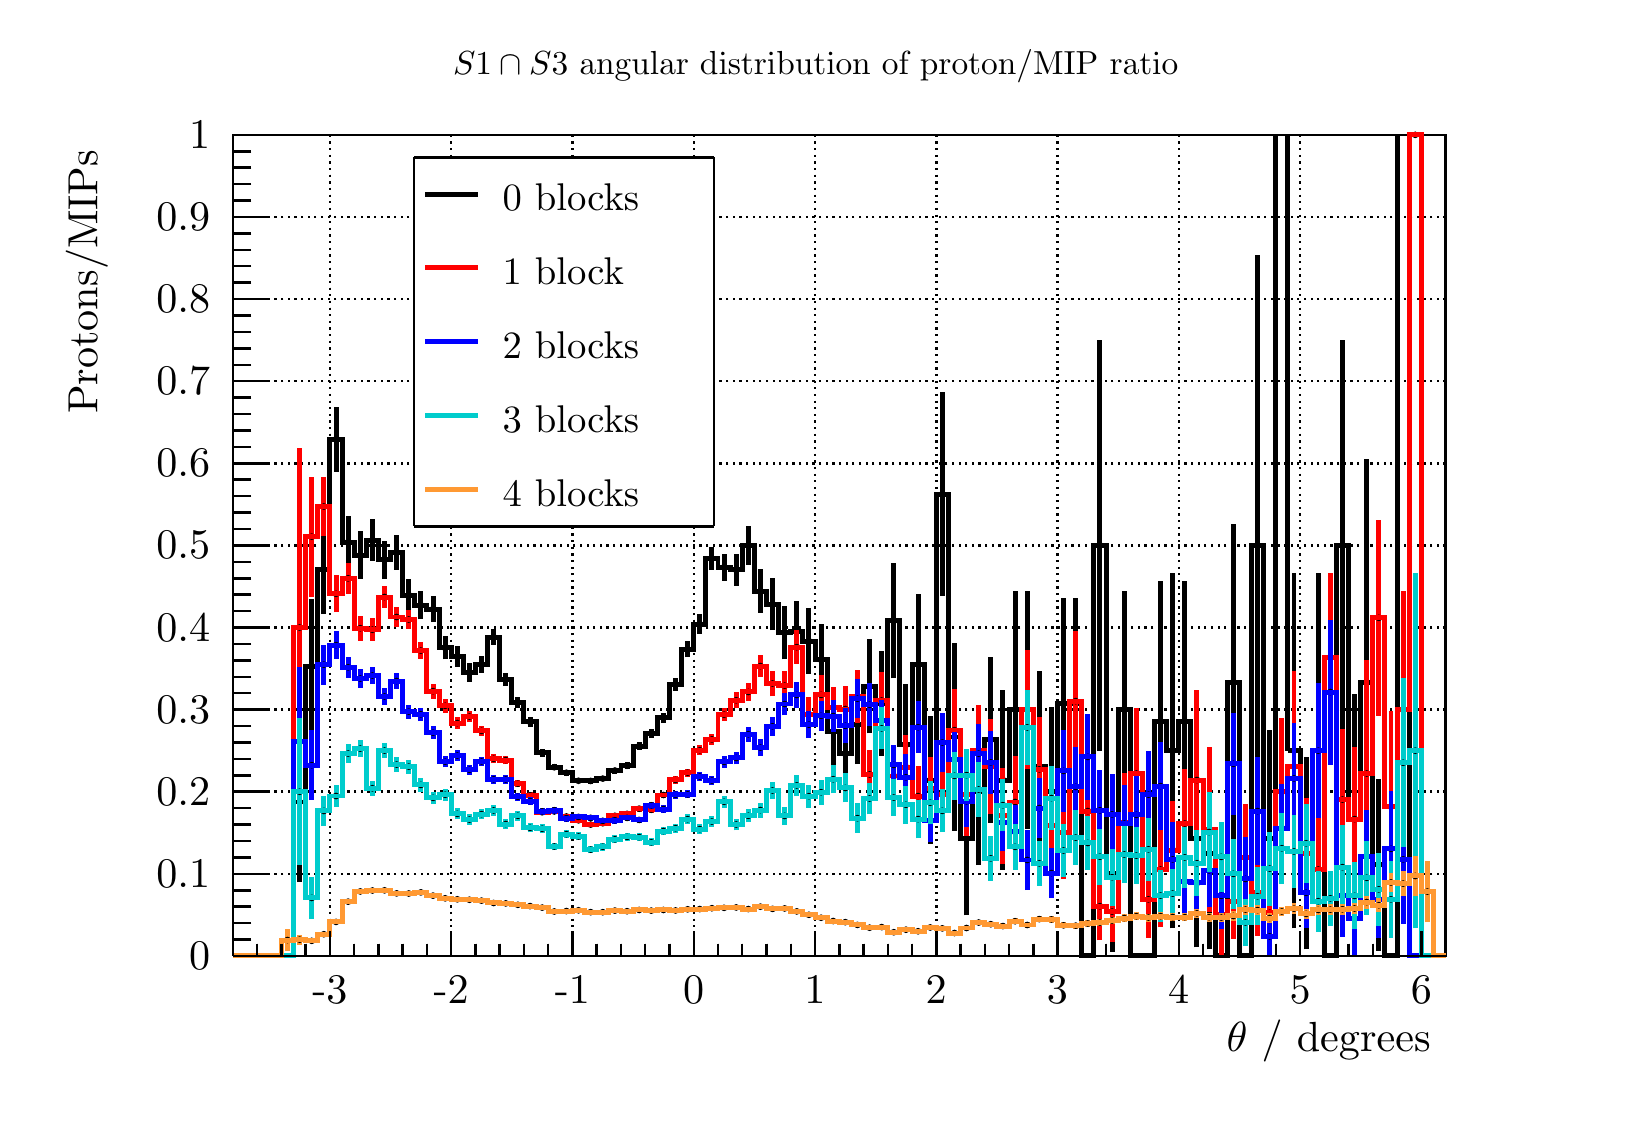
\begin{tikzpicture}
\pgfdeclareplotmark{cross} {
\pgfpathmoveto{\pgfpoint{-0.3\pgfplotmarksize}{\pgfplotmarksize}}
\pgfpathlineto{\pgfpoint{+0.3\pgfplotmarksize}{\pgfplotmarksize}}
\pgfpathlineto{\pgfpoint{+0.3\pgfplotmarksize}{0.3\pgfplotmarksize}}
\pgfpathlineto{\pgfpoint{+1\pgfplotmarksize}{0.3\pgfplotmarksize}}
\pgfpathlineto{\pgfpoint{+1\pgfplotmarksize}{-0.3\pgfplotmarksize}}
\pgfpathlineto{\pgfpoint{+0.3\pgfplotmarksize}{-0.3\pgfplotmarksize}}
\pgfpathlineto{\pgfpoint{+0.3\pgfplotmarksize}{-1.\pgfplotmarksize}}
\pgfpathlineto{\pgfpoint{-0.3\pgfplotmarksize}{-1.\pgfplotmarksize}}
\pgfpathlineto{\pgfpoint{-0.3\pgfplotmarksize}{-0.3\pgfplotmarksize}}
\pgfpathlineto{\pgfpoint{-1.\pgfplotmarksize}{-0.3\pgfplotmarksize}}
\pgfpathlineto{\pgfpoint{-1.\pgfplotmarksize}{0.3\pgfplotmarksize}}
\pgfpathlineto{\pgfpoint{-0.3\pgfplotmarksize}{0.3\pgfplotmarksize}}
\pgfpathclose
\pgfusepathqstroke
}
\pgfdeclareplotmark{cross*} {
\pgfpathmoveto{\pgfpoint{-0.3\pgfplotmarksize}{\pgfplotmarksize}}
\pgfpathlineto{\pgfpoint{+0.3\pgfplotmarksize}{\pgfplotmarksize}}
\pgfpathlineto{\pgfpoint{+0.3\pgfplotmarksize}{0.3\pgfplotmarksize}}
\pgfpathlineto{\pgfpoint{+1\pgfplotmarksize}{0.3\pgfplotmarksize}}
\pgfpathlineto{\pgfpoint{+1\pgfplotmarksize}{-0.3\pgfplotmarksize}}
\pgfpathlineto{\pgfpoint{+0.3\pgfplotmarksize}{-0.3\pgfplotmarksize}}
\pgfpathlineto{\pgfpoint{+0.3\pgfplotmarksize}{-1.\pgfplotmarksize}}
\pgfpathlineto{\pgfpoint{-0.3\pgfplotmarksize}{-1.\pgfplotmarksize}}
\pgfpathlineto{\pgfpoint{-0.3\pgfplotmarksize}{-0.3\pgfplotmarksize}}
\pgfpathlineto{\pgfpoint{-1.\pgfplotmarksize}{-0.3\pgfplotmarksize}}
\pgfpathlineto{\pgfpoint{-1.\pgfplotmarksize}{0.3\pgfplotmarksize}}
\pgfpathlineto{\pgfpoint{-0.3\pgfplotmarksize}{0.3\pgfplotmarksize}}
\pgfpathclose
\pgfusepathqfillstroke
}
\pgfdeclareplotmark{newstar} {
\pgfpathmoveto{\pgfqpoint{0pt}{\pgfplotmarksize}}
\pgfpathlineto{\pgfqpointpolar{44}{0.5\pgfplotmarksize}}
\pgfpathlineto{\pgfqpointpolar{18}{\pgfplotmarksize}}
\pgfpathlineto{\pgfqpointpolar{-20}{0.5\pgfplotmarksize}}
\pgfpathlineto{\pgfqpointpolar{-54}{\pgfplotmarksize}}
\pgfpathlineto{\pgfqpointpolar{-90}{0.5\pgfplotmarksize}}
\pgfpathlineto{\pgfqpointpolar{234}{\pgfplotmarksize}}
\pgfpathlineto{\pgfqpointpolar{198}{0.5\pgfplotmarksize}}
\pgfpathlineto{\pgfqpointpolar{162}{\pgfplotmarksize}}
\pgfpathlineto{\pgfqpointpolar{134}{0.5\pgfplotmarksize}}
\pgfpathclose
\pgfusepathqstroke
}
\pgfdeclareplotmark{newstar*} {
\pgfpathmoveto{\pgfqpoint{0pt}{\pgfplotmarksize}}
\pgfpathlineto{\pgfqpointpolar{44}{0.5\pgfplotmarksize}}
\pgfpathlineto{\pgfqpointpolar{18}{\pgfplotmarksize}}
\pgfpathlineto{\pgfqpointpolar{-20}{0.5\pgfplotmarksize}}
\pgfpathlineto{\pgfqpointpolar{-54}{\pgfplotmarksize}}
\pgfpathlineto{\pgfqpointpolar{-90}{0.5\pgfplotmarksize}}
\pgfpathlineto{\pgfqpointpolar{234}{\pgfplotmarksize}}
\pgfpathlineto{\pgfqpointpolar{198}{0.5\pgfplotmarksize}}
\pgfpathlineto{\pgfqpointpolar{162}{\pgfplotmarksize}}
\pgfpathlineto{\pgfqpointpolar{134}{0.5\pgfplotmarksize}}
\pgfpathclose
\pgfusepathqfillstroke
}
\definecolor{c}{rgb}{1,1,1};
\draw [color=c, fill=c] (0,0) rectangle (20,13.5429);
\draw [color=c, fill=c] (2.6,1.76057) rectangle (18,12.1886);
\definecolor{c}{rgb}{0,0,0};
\draw [c,line width=0.9] (2.6,1.76057) -- (2.6,12.1886) -- (18,12.1886) -- (18,1.76057) -- (2.6,1.76057);
\definecolor{c}{rgb}{1,1,1};
\draw [color=c, fill=c] (2.6,1.76057) rectangle (18,12.1886);
\definecolor{c}{rgb}{0,0,0};
\draw [c,line width=0.9] (2.6,1.76057) -- (2.6,12.1886) -- (18,12.1886) -- (18,1.76057) -- (2.6,1.76057);
\draw [c,line width=0.9] (2.6,1.76057) -- (18,1.76057);
\draw [c,dash pattern=on 0.80pt off 1.60pt ,line width=0.9] (3.832,12.1886) -- (3.832,1.76057);
\draw [c,dash pattern=on 0.80pt off 1.60pt ,line width=0.9] (5.372,12.1886) -- (5.372,1.76057);
\draw [c,dash pattern=on 0.80pt off 1.60pt ,line width=0.9] (6.912,12.1886) -- (6.912,1.76057);
\draw [c,dash pattern=on 0.80pt off 1.60pt ,line width=0.9] (8.452,12.1886) -- (8.452,1.76057);
\draw [c,dash pattern=on 0.80pt off 1.60pt ,line width=0.9] (9.992,12.1886) -- (9.992,1.76057);
\draw [c,dash pattern=on 0.80pt off 1.60pt ,line width=0.9] (11.532,12.1886) -- (11.532,1.76057);
\draw [c,dash pattern=on 0.80pt off 1.60pt ,line width=0.9] (13.072,12.1886) -- (13.072,1.76057);
\draw [c,dash pattern=on 0.80pt off 1.60pt ,line width=0.9] (14.612,12.1886) -- (14.612,1.76057);
\draw [c,dash pattern=on 0.80pt off 1.60pt ,line width=0.9] (16.152,12.1886) -- (16.152,1.76057);
\draw [c,dash pattern=on 0.80pt off 1.60pt ,line width=0.9] (17.692,12.1886) -- (17.692,1.76057);
\draw [c,dash pattern=on 0.80pt off 1.60pt ,line width=0.9] (3.832,12.1886) -- (3.832,1.76057);
\draw [c,dash pattern=on 0.80pt off 1.60pt ,line width=0.9] (17.692,12.1886) -- (17.692,1.76057);
\draw [c,line width=0.9] (2.6,1.76057) -- (2.6,12.1886);
\draw [c,dash pattern=on 0.80pt off 1.60pt ,line width=0.9] (18,1.76057) -- (2.6,1.76057);
\draw [c,dash pattern=on 0.80pt off 1.60pt ,line width=0.9] (18,2.80337) -- (2.6,2.80337);
\draw [c,dash pattern=on 0.80pt off 1.60pt ,line width=0.9] (18,3.84617) -- (2.6,3.84617);
\draw [c,dash pattern=on 0.80pt off 1.60pt ,line width=0.9] (18,4.88897) -- (2.6,4.88897);
\draw [c,dash pattern=on 0.80pt off 1.60pt ,line width=0.9] (18,5.93177) -- (2.6,5.93177);
\draw [c,dash pattern=on 0.80pt off 1.60pt ,line width=0.9] (18,6.97457) -- (2.6,6.97457);
\draw [c,dash pattern=on 0.80pt off 1.60pt ,line width=0.9] (18,8.01737) -- (2.6,8.01737);
\draw [c,dash pattern=on 0.80pt off 1.60pt ,line width=0.9] (18,9.06017) -- (2.6,9.06017);
\draw [c,dash pattern=on 0.80pt off 1.60pt ,line width=0.9] (18,10.103) -- (2.6,10.103);
\draw [c,dash pattern=on 0.80pt off 1.60pt ,line width=0.9] (18,11.1458) -- (2.6,11.1458);
\draw [c,dash pattern=on 0.80pt off 1.60pt ,line width=0.9] (18,12.1886) -- (2.6,12.1886);
\definecolor{c}{rgb}{0,0,0.6};
\draw [c,line width=0.9] (2.6,1.76057) -- (2.754,1.76057) -- (2.754,1.76057) -- (2.908,1.76057) -- (2.908,1.76057) -- (3.062,1.76057) -- (3.062,1.76057) -- (3.216,1.76057) -- (3.216,1.76057) -- (3.37,1.76057) -- (3.37,1.76057) -- (3.524,1.76057) --
 (3.524,1.76057) -- (3.678,1.76057) -- (3.678,1.76057) -- (3.832,1.76057) -- (3.832,1.76057) -- (3.986,1.76057) -- (3.986,1.76057) -- (4.14,1.76057) -- (4.14,1.76057) -- (4.294,1.76057) -- (4.294,1.76057) -- (4.448,1.76057) -- (4.448,1.76057) --
 (4.602,1.76057) -- (4.602,1.76057) -- (4.756,1.76057) -- (4.756,1.76057) -- (4.91,1.76057) -- (4.91,1.76057) -- (5.064,1.76057) -- (5.064,1.76057) -- (5.218,1.76057) -- (5.218,1.76057) -- (5.372,1.76057) -- (5.372,1.76057) -- (5.526,1.76057) --
 (5.526,1.76057) -- (5.68,1.76057) -- (5.68,1.76057) -- (5.834,1.76057) -- (5.834,1.76057) -- (5.988,1.76057) -- (5.988,1.76057) -- (6.142,1.76057) -- (6.142,1.76057) -- (6.296,1.76057) -- (6.296,1.76057) -- (6.45,1.76057) -- (6.45,1.76057) --
 (6.604,1.76057) -- (6.604,1.76057) -- (6.758,1.76057) -- (6.758,1.76057) -- (6.912,1.76057) -- (6.912,1.76057) -- (7.066,1.76057) -- (7.066,1.76057) -- (7.22,1.76057) -- (7.22,1.76057) -- (7.374,1.76057) -- (7.374,1.76057) -- (7.528,1.76057) --
 (7.528,1.76057) -- (7.682,1.76057) -- (7.682,1.76057) -- (7.836,1.76057) -- (7.836,1.76057) -- (7.99,1.76057) -- (7.99,1.76057) -- (8.144,1.76057) -- (8.144,1.76057) -- (8.298,1.76057) -- (8.298,1.76057) -- (8.452,1.76057) -- (8.452,1.76057) --
 (8.606,1.76057) -- (8.606,1.76057) -- (8.76,1.76057) -- (8.76,1.76057) -- (8.914,1.76057) -- (8.914,1.76057) -- (9.068,1.76057) -- (9.068,1.76057) -- (9.222,1.76057) -- (9.222,1.76057) -- (9.376,1.76057) -- (9.376,1.76057) -- (9.53,1.76057) --
 (9.53,1.76057) -- (9.684,1.76057) -- (9.684,1.76057) -- (9.838,1.76057) -- (9.838,1.76057) -- (9.992,1.76057) -- (9.992,1.76057) -- (10.146,1.76057) -- (10.146,1.76057) -- (10.3,1.76057) -- (10.3,1.76057) -- (10.454,1.76057) -- (10.454,1.76057) --
 (10.608,1.76057) -- (10.608,1.76057) -- (10.762,1.76057) -- (10.762,1.76057) -- (10.916,1.76057) -- (10.916,1.76057) -- (11.07,1.76057) -- (11.07,1.76057) -- (11.224,1.76057) -- (11.224,1.76057) -- (11.378,1.76057) -- (11.378,1.76057) --
 (11.532,1.76057) -- (11.532,1.76057) -- (11.686,1.76057) -- (11.686,1.76057) -- (11.84,1.76057) -- (11.84,1.76057) -- (11.994,1.76057) -- (11.994,1.76057) -- (12.148,1.76057) -- (12.148,1.76057) -- (12.302,1.76057) -- (12.302,1.76057) --
 (12.456,1.76057) -- (12.456,1.76057) -- (12.61,1.76057) -- (12.61,1.76057) -- (12.764,1.76057) -- (12.764,1.76057) -- (12.918,1.76057) -- (12.918,1.76057) -- (13.072,1.76057) -- (13.072,1.76057) -- (13.226,1.76057) -- (13.226,1.76057) --
 (13.38,1.76057) -- (13.38,1.76057) -- (13.534,1.76057) -- (13.534,1.76057) -- (13.688,1.76057) -- (13.688,1.76057) -- (13.842,1.76057) -- (13.842,1.76057) -- (13.996,1.76057) -- (13.996,1.76057) -- (14.15,1.76057) -- (14.15,1.76057) --
 (14.304,1.76057) -- (14.304,1.76057) -- (14.458,1.76057) -- (14.458,1.76057) -- (14.612,1.76057) -- (14.612,1.76057) -- (14.766,1.76057) -- (14.766,1.76057) -- (14.92,1.76057) -- (14.92,1.76057) -- (15.074,1.76057) -- (15.074,1.76057) --
 (15.228,1.76057) -- (15.228,1.76057) -- (15.382,1.76057) -- (15.382,1.76057) -- (15.536,1.76057) -- (15.536,1.76057) -- (15.69,1.76057) -- (15.69,1.76057) -- (15.844,1.76057) -- (15.844,1.76057) -- (15.998,1.76057) -- (15.998,1.76057) --
 (16.152,1.76057) -- (16.152,1.76057) -- (16.306,1.76057) -- (16.306,1.76057) -- (16.46,1.76057) -- (16.46,1.76057) -- (16.614,1.76057) -- (16.614,1.76057) -- (16.768,1.76057) -- (16.768,1.76057) -- (16.922,1.76057) -- (16.922,1.76057) --
 (17.076,1.76057) -- (17.076,1.76057) -- (17.23,1.76057) -- (17.23,1.76057) -- (17.384,1.76057) -- (17.384,1.76057) -- (17.538,1.76057) -- (17.538,1.76057) -- (17.692,1.76057) -- (17.692,1.76057) -- (17.846,1.76057) -- (17.846,1.76057) --
 (18,1.76057);
\definecolor{c}{rgb}{0,0,0};
\draw [c,line width=0.9] (2.6,1.76057) -- (18,1.76057);
\draw [c,line width=0.9] (3.832,2.07341) -- (3.832,1.76057);
\draw [c,line width=0.9] (4.14,1.91699) -- (4.14,1.76057);
\draw [c,line width=0.9] (4.448,1.91699) -- (4.448,1.76057);
\draw [c,line width=0.9] (4.756,1.91699) -- (4.756,1.76057);
\draw [c,line width=0.9] (5.064,1.91699) -- (5.064,1.76057);
\draw [c,line width=0.9] (5.372,2.07341) -- (5.372,1.76057);
\draw [c,line width=0.9] (5.68,1.91699) -- (5.68,1.76057);
\draw [c,line width=0.9] (5.988,1.91699) -- (5.988,1.76057);
\draw [c,line width=0.9] (6.296,1.91699) -- (6.296,1.76057);
\draw [c,line width=0.9] (6.604,1.91699) -- (6.604,1.76057);
\draw [c,line width=0.9] (6.912,2.07341) -- (6.912,1.76057);
\draw [c,line width=0.9] (7.22,1.91699) -- (7.22,1.76057);
\draw [c,line width=0.9] (7.528,1.91699) -- (7.528,1.76057);
\draw [c,line width=0.9] (7.836,1.91699) -- (7.836,1.76057);
\draw [c,line width=0.9] (8.144,1.91699) -- (8.144,1.76057);
\draw [c,line width=0.9] (8.452,2.07341) -- (8.452,1.76057);
\draw [c,line width=0.9] (8.76,1.91699) -- (8.76,1.76057);
\draw [c,line width=0.9] (9.068,1.91699) -- (9.068,1.76057);
\draw [c,line width=0.9] (9.376,1.91699) -- (9.376,1.76057);
\draw [c,line width=0.9] (9.684,1.91699) -- (9.684,1.76057);
\draw [c,line width=0.9] (9.992,2.07341) -- (9.992,1.76057);
\draw [c,line width=0.9] (10.3,1.91699) -- (10.3,1.76057);
\draw [c,line width=0.9] (10.608,1.91699) -- (10.608,1.76057);
\draw [c,line width=0.9] (10.916,1.91699) -- (10.916,1.76057);
\draw [c,line width=0.9] (11.224,1.91699) -- (11.224,1.76057);
\draw [c,line width=0.9] (11.532,2.07341) -- (11.532,1.76057);
\draw [c,line width=0.9] (11.84,1.91699) -- (11.84,1.76057);
\draw [c,line width=0.9] (12.148,1.91699) -- (12.148,1.76057);
\draw [c,line width=0.9] (12.456,1.91699) -- (12.456,1.76057);
\draw [c,line width=0.9] (12.764,1.91699) -- (12.764,1.76057);
\draw [c,line width=0.9] (13.072,2.07341) -- (13.072,1.76057);
\draw [c,line width=0.9] (13.38,1.91699) -- (13.38,1.76057);
\draw [c,line width=0.9] (13.688,1.91699) -- (13.688,1.76057);
\draw [c,line width=0.9] (13.996,1.91699) -- (13.996,1.76057);
\draw [c,line width=0.9] (14.304,1.91699) -- (14.304,1.76057);
\draw [c,line width=0.9] (14.612,2.07341) -- (14.612,1.76057);
\draw [c,line width=0.9] (14.92,1.91699) -- (14.92,1.76057);
\draw [c,line width=0.9] (15.228,1.91699) -- (15.228,1.76057);
\draw [c,line width=0.9] (15.536,1.91699) -- (15.536,1.76057);
\draw [c,line width=0.9] (15.844,1.91699) -- (15.844,1.76057);
\draw [c,line width=0.9] (16.152,2.07341) -- (16.152,1.76057);
\draw [c,line width=0.9] (16.46,1.91699) -- (16.46,1.76057);
\draw [c,line width=0.9] (16.768,1.91699) -- (16.768,1.76057);
\draw [c,line width=0.9] (17.076,1.91699) -- (17.076,1.76057);
\draw [c,line width=0.9] (17.384,1.91699) -- (17.384,1.76057);
\draw [c,line width=0.9] (17.692,2.07341) -- (17.692,1.76057);
\draw [c,line width=0.9] (3.832,2.07341) -- (3.832,1.76057);
\draw [c,line width=0.9] (3.524,1.91699) -- (3.524,1.76057);
\draw [c,line width=0.9] (3.216,1.91699) -- (3.216,1.76057);
\draw [c,line width=0.9] (2.908,1.91699) -- (2.908,1.76057);
\draw [c,line width=0.9] (17.692,2.07341) -- (17.692,1.76057);
\draw [anchor=base] (3.832,1.15114) node[scale=1.52295, color=c, rotate=0]{-3};
\draw [anchor=base] (5.372,1.15114) node[scale=1.52295, color=c, rotate=0]{-2};
\draw [anchor=base] (6.912,1.15114) node[scale=1.52295, color=c, rotate=0]{-1};
\draw [anchor=base] (8.452,1.15114) node[scale=1.52295, color=c, rotate=0]{0};
\draw [anchor=base] (9.992,1.15114) node[scale=1.52295, color=c, rotate=0]{1};
\draw [anchor=base] (11.532,1.15114) node[scale=1.52295, color=c, rotate=0]{2};
\draw [anchor=base] (13.072,1.15114) node[scale=1.52295, color=c, rotate=0]{3};
\draw [anchor=base] (14.612,1.15114) node[scale=1.52295, color=c, rotate=0]{4};
\draw [anchor=base] (16.152,1.15114) node[scale=1.52295, color=c, rotate=0]{5};
\draw [anchor=base] (17.692,1.15114) node[scale=1.52295, color=c, rotate=0]{6};
\draw [anchor= east] (18,0.677143) node[scale=1.52295, color=c, rotate=0]{$ \theta$ / degrees};
\draw [c,line width=0.9] (2.6,1.76057) -- (2.6,12.1886);
\draw [c,line width=0.9] (3.062,1.76057) -- (2.6,1.76057);
\draw [c,line width=0.9] (2.831,1.96913) -- (2.6,1.96913);
\draw [c,line width=0.9] (2.831,2.17769) -- (2.6,2.17769);
\draw [c,line width=0.9] (2.831,2.38625) -- (2.6,2.38625);
\draw [c,line width=0.9] (2.831,2.59481) -- (2.6,2.59481);
\draw [c,line width=0.9] (3.062,2.80337) -- (2.6,2.80337);
\draw [c,line width=0.9] (2.831,3.01193) -- (2.6,3.01193);
\draw [c,line width=0.9] (2.831,3.22049) -- (2.6,3.22049);
\draw [c,line width=0.9] (2.831,3.42905) -- (2.6,3.42905);
\draw [c,line width=0.9] (2.831,3.63761) -- (2.6,3.63761);
\draw [c,line width=0.9] (3.062,3.84617) -- (2.6,3.84617);
\draw [c,line width=0.9] (2.831,4.05473) -- (2.6,4.05473);
\draw [c,line width=0.9] (2.831,4.26329) -- (2.6,4.26329);
\draw [c,line width=0.9] (2.831,4.47185) -- (2.6,4.47185);
\draw [c,line width=0.9] (2.831,4.68041) -- (2.6,4.68041);
\draw [c,line width=0.9] (3.062,4.88897) -- (2.6,4.88897);
\draw [c,line width=0.9] (2.831,5.09753) -- (2.6,5.09753);
\draw [c,line width=0.9] (2.831,5.30609) -- (2.6,5.30609);
\draw [c,line width=0.9] (2.831,5.51465) -- (2.6,5.51465);
\draw [c,line width=0.9] (2.831,5.72321) -- (2.6,5.72321);
\draw [c,line width=0.9] (3.062,5.93177) -- (2.6,5.93177);
\draw [c,line width=0.9] (2.831,6.14033) -- (2.6,6.14033);
\draw [c,line width=0.9] (2.831,6.34889) -- (2.6,6.34889);
\draw [c,line width=0.9] (2.831,6.55745) -- (2.6,6.55745);
\draw [c,line width=0.9] (2.831,6.76601) -- (2.6,6.76601);
\draw [c,line width=0.9] (3.062,6.97457) -- (2.6,6.97457);
\draw [c,line width=0.9] (2.831,7.18313) -- (2.6,7.18313);
\draw [c,line width=0.9] (2.831,7.39169) -- (2.6,7.39169);
\draw [c,line width=0.9] (2.831,7.60025) -- (2.6,7.60025);
\draw [c,line width=0.9] (2.831,7.80881) -- (2.6,7.80881);
\draw [c,line width=0.9] (3.062,8.01737) -- (2.6,8.01737);
\draw [c,line width=0.9] (2.831,8.22593) -- (2.6,8.22593);
\draw [c,line width=0.9] (2.831,8.43449) -- (2.6,8.43449);
\draw [c,line width=0.9] (2.831,8.64305) -- (2.6,8.64305);
\draw [c,line width=0.9] (2.831,8.85161) -- (2.6,8.85161);
\draw [c,line width=0.9] (3.062,9.06017) -- (2.6,9.06017);
\draw [c,line width=0.9] (2.831,9.26873) -- (2.6,9.26873);
\draw [c,line width=0.9] (2.831,9.47729) -- (2.6,9.47729);
\draw [c,line width=0.9] (2.831,9.68585) -- (2.6,9.68585);
\draw [c,line width=0.9] (2.831,9.89441) -- (2.6,9.89441);
\draw [c,line width=0.9] (3.062,10.103) -- (2.6,10.103);
\draw [c,line width=0.9] (2.831,10.3115) -- (2.6,10.3115);
\draw [c,line width=0.9] (2.831,10.5201) -- (2.6,10.5201);
\draw [c,line width=0.9] (2.831,10.7287) -- (2.6,10.7287);
\draw [c,line width=0.9] (2.831,10.9372) -- (2.6,10.9372);
\draw [c,line width=0.9] (3.062,11.1458) -- (2.6,11.1458);
\draw [c,line width=0.9] (2.831,11.3543) -- (2.6,11.3543);
\draw [c,line width=0.9] (2.831,11.5629) -- (2.6,11.5629);
\draw [c,line width=0.9] (2.831,11.7715) -- (2.6,11.7715);
\draw [c,line width=0.9] (2.831,11.98) -- (2.6,11.98);
\draw [c,line width=0.9] (3.062,12.1886) -- (2.6,12.1886);
\draw [anchor= east] (2.5,1.76057) node[scale=1.52295, color=c, rotate=0]{0};
\draw [anchor= east] (2.5,2.80337) node[scale=1.52295, color=c, rotate=0]{0.1};
\draw [anchor= east] (2.5,3.84617) node[scale=1.52295, color=c, rotate=0]{0.2};
\draw [anchor= east] (2.5,4.88897) node[scale=1.52295, color=c, rotate=0]{0.3};
\draw [anchor= east] (2.5,5.93177) node[scale=1.52295, color=c, rotate=0]{0.4};
\draw [anchor= east] (2.5,6.97457) node[scale=1.52295, color=c, rotate=0]{0.5};
\draw [anchor= east] (2.5,8.01737) node[scale=1.52295, color=c, rotate=0]{0.6};
\draw [anchor= east] (2.5,9.06017) node[scale=1.52295, color=c, rotate=0]{0.7};
\draw [anchor= east] (2.5,10.103) node[scale=1.52295, color=c, rotate=0]{0.8};
\draw [anchor= east] (2.5,11.1458) node[scale=1.52295, color=c, rotate=0]{0.9};
\draw [anchor= east] (2.5,12.1886) node[scale=1.52295, color=c, rotate=0]{1};
\draw [anchor= east] (0.742857,12.1886) node[scale=1.52295, color=c, rotate=90]{  Protons/MIPs};
\draw [c,line width=1.8] (3.447,2.69828) -- (3.447,3.71582);
\draw [c,line width=1.8] (3.447,3.71582) -- (3.447,4.73337);
\foreach \P in {(3.447,3.71582)}{\draw[mark options={color=c,fill=c},mark size=2.402402pt,mark=*,mark size=1pt] plot coordinates {\P};}
\draw [c,line width=1.8] (3.601,4.5864) -- (3.601,5.44104);
\draw [c,line width=1.8] (3.601,5.44104) -- (3.601,6.29568);
\foreach \P in {(3.601,5.44104)}{\draw[mark options={color=c,fill=c},mark size=2.402402pt,mark=*,mark size=1pt] plot coordinates {\P};}
\draw [c,line width=1.8] (3.755,6.10331) -- (3.755,6.66787);
\draw [c,line width=1.8] (3.755,6.66787) -- (3.755,7.23242);
\foreach \P in {(3.755,6.66787)}{\draw[mark options={color=c,fill=c},mark size=2.402402pt,mark=*,mark size=1pt] plot coordinates {\P};}
\draw [c,line width=1.8] (3.909,7.91132) -- (3.909,8.32123);
\draw [c,line width=1.8] (3.909,8.32123) -- (3.909,8.73115);
\foreach \P in {(3.909,8.32123)}{\draw[mark options={color=c,fill=c},mark size=2.402402pt,mark=*,mark size=1pt] plot coordinates {\P};}
\draw [c,line width=1.8] (4.063,6.68653) -- (4.063,7.01628);
\draw [c,line width=1.8] (4.063,7.01628) -- (4.063,7.34604);
\foreach \P in {(4.063,7.01628)}{\draw[mark options={color=c,fill=c},mark size=2.402402pt,mark=*,mark size=1pt] plot coordinates {\P};}
\draw [c,line width=1.8] (4.217,6.54736) -- (4.217,6.85085);
\draw [c,line width=1.8] (4.217,6.85085) -- (4.217,7.15433);
\foreach \P in {(4.217,6.85085)}{\draw[mark options={color=c,fill=c},mark size=2.402402pt,mark=*,mark size=1pt] plot coordinates {\P};}
\draw [c,line width=1.8] (4.371,6.77692) -- (4.371,7.04194);
\draw [c,line width=1.8] (4.371,7.04194) -- (4.371,7.30696);
\foreach \P in {(4.371,7.04194)}{\draw[mark options={color=c,fill=c},mark size=2.402402pt,mark=*,mark size=1pt] plot coordinates {\P};}
\draw [c,line width=1.8] (4.525,6.54627) -- (4.525,6.79082);
\draw [c,line width=1.8] (4.525,6.79082) -- (4.525,7.03537);
\foreach \P in {(4.525,6.79082)}{\draw[mark options={color=c,fill=c},mark size=2.402402pt,mark=*,mark size=1pt] plot coordinates {\P};}
\draw [c,line width=1.8] (4.679,6.66261) -- (4.679,6.88212);
\draw [c,line width=1.8] (4.679,6.88212) -- (4.679,7.10164);
\foreach \P in {(4.679,6.88212)}{\draw[mark options={color=c,fill=c},mark size=2.402402pt,mark=*,mark size=1pt] plot coordinates {\P};}
\draw [c,line width=1.8] (4.833,6.14124) -- (4.833,6.34378);
\draw [c,line width=1.8] (4.833,6.34378) -- (4.833,6.54632);
\foreach \P in {(4.833,6.34378)}{\draw[mark options={color=c,fill=c},mark size=2.402402pt,mark=*,mark size=1pt] plot coordinates {\P};}
\draw [c,line width=1.8] (4.987,6.03439) -- (4.987,6.21354);
\draw [c,line width=1.8] (4.987,6.21354) -- (4.987,6.39269);
\foreach \P in {(4.987,6.21354)}{\draw[mark options={color=c,fill=c},mark size=2.402402pt,mark=*,mark size=1pt] plot coordinates {\P};}
\draw [c,line width=1.8] (5.141,6.00133) -- (5.141,6.16587);
\draw [c,line width=1.8] (5.141,6.16587) -- (5.141,6.33041);
\foreach \P in {(5.141,6.16587)}{\draw[mark options={color=c,fill=c},mark size=2.402402pt,mark=*,mark size=1pt] plot coordinates {\P};}
\draw [c,line width=1.8] (5.295,5.52618) -- (5.295,5.67328);
\draw [c,line width=1.8] (5.295,5.67328) -- (5.295,5.82039);
\foreach \P in {(5.295,5.67328)}{\draw[mark options={color=c,fill=c},mark size=2.402402pt,mark=*,mark size=1pt] plot coordinates {\P};}
\draw [c,line width=1.8] (5.449,5.43471) -- (5.449,5.5688);
\draw [c,line width=1.8] (5.449,5.5688) -- (5.449,5.70289);
\foreach \P in {(5.449,5.5688)}{\draw[mark options={color=c,fill=c},mark size=2.402402pt,mark=*,mark size=1pt] plot coordinates {\P};}
\draw [c,line width=1.8] (5.603,5.24489) -- (5.603,5.36319);
\draw [c,line width=1.8] (5.603,5.36319) -- (5.603,5.48149);
\foreach \P in {(5.603,5.36319)}{\draw[mark options={color=c,fill=c},mark size=2.402402pt,mark=*,mark size=1pt] plot coordinates {\P};}
\draw [c,line width=1.8] (5.757,5.35586) -- (5.757,5.46365);
\draw [c,line width=1.8] (5.757,5.46365) -- (5.757,5.57145);
\foreach \P in {(5.757,5.46365)}{\draw[mark options={color=c,fill=c},mark size=2.402402pt,mark=*,mark size=1pt] plot coordinates {\P};}
\draw [c,line width=1.8] (5.911,5.71068) -- (5.911,5.80974);
\draw [c,line width=1.8] (5.911,5.80974) -- (5.911,5.9088);
\foreach \P in {(5.911,5.80974)}{\draw[mark options={color=c,fill=c},mark size=2.402402pt,mark=*,mark size=1pt] plot coordinates {\P};}
\draw [c,line width=1.8] (6.065,5.18882) -- (6.065,5.27358);
\draw [c,line width=1.8] (6.065,5.27358) -- (6.065,5.35835);
\foreach \P in {(6.065,5.27358)}{\draw[mark options={color=c,fill=c},mark size=2.402402pt,mark=*,mark size=1pt] plot coordinates {\P};}
\draw [c,line width=1.8] (6.219,4.90855) -- (6.219,4.97895);
\draw [c,line width=1.8] (6.219,4.97895) -- (6.219,5.04935);
\foreach \P in {(6.219,4.97895)}{\draw[mark options={color=c,fill=c},mark size=2.402402pt,mark=*,mark size=1pt] plot coordinates {\P};}
\draw [c,line width=1.8] (6.373,4.67359) -- (6.373,4.73253);
\draw [c,line width=1.8] (6.373,4.73253) -- (6.373,4.79147);
\foreach \P in {(6.373,4.73253)}{\draw[mark options={color=c,fill=c},mark size=2.402402pt,mark=*,mark size=1pt] plot coordinates {\P};}
\draw [c,line width=1.8] (6.527,4.29323) -- (6.527,4.34135);
\draw [c,line width=1.8] (6.527,4.34135) -- (6.527,4.38946);
\foreach \P in {(6.527,4.34135)}{\draw[mark options={color=c,fill=c},mark size=2.402402pt,mark=*,mark size=1pt] plot coordinates {\P};}
\draw [c,line width=1.8] (6.681,4.11642) -- (6.681,4.1571);
\draw [c,line width=1.8] (6.681,4.1571) -- (6.681,4.19778);
\foreach \P in {(6.681,4.1571)}{\draw[mark options={color=c,fill=c},mark size=2.402402pt,mark=*,mark size=1pt] plot coordinates {\P};}
\draw [c,line width=1.8] (6.835,4.05142) -- (6.835,4.08804);
\draw [c,line width=1.8] (6.835,4.08804) -- (6.835,4.12465);
\foreach \P in {(6.835,4.08804)}{\draw[mark options={color=c,fill=c},mark size=2.402402pt,mark=*,mark size=1pt] plot coordinates {\P};}
\draw [c,line width=1.8] (6.989,3.95156) -- (6.989,3.98547);
\draw [c,line width=1.8] (6.989,3.98547) -- (6.989,4.01939);
\foreach \P in {(6.989,3.98547)}{\draw[mark options={color=c,fill=c},mark size=2.402402pt,mark=*,mark size=1pt] plot coordinates {\P};}
\draw [c,line width=1.8] (7.143,3.94992) -- (7.143,3.98352);
\draw [c,line width=1.8] (7.143,3.98352) -- (7.143,4.01712);
\foreach \P in {(7.143,3.98352)}{\draw[mark options={color=c,fill=c},mark size=2.402402pt,mark=*,mark size=1pt] plot coordinates {\P};}
\draw [c,line width=1.8] (7.297,3.97822) -- (7.297,4.013);
\draw [c,line width=1.8] (7.297,4.013) -- (7.297,4.04777);
\foreach \P in {(7.297,4.013)}{\draw[mark options={color=c,fill=c},mark size=2.402402pt,mark=*,mark size=1pt] plot coordinates {\P};}
\draw [c,line width=1.8] (7.451,4.07786) -- (7.451,4.11597);
\draw [c,line width=1.8] (7.451,4.11597) -- (7.451,4.15409);
\foreach \P in {(7.451,4.11597)}{\draw[mark options={color=c,fill=c},mark size=2.402402pt,mark=*,mark size=1pt] plot coordinates {\P};}
\draw [c,line width=1.8] (7.605,4.13387) -- (7.605,4.17615);
\draw [c,line width=1.8] (7.605,4.17615) -- (7.605,4.21843);
\foreach \P in {(7.605,4.17615)}{\draw[mark options={color=c,fill=c},mark size=2.402402pt,mark=*,mark size=1pt] plot coordinates {\P};}
\draw [c,line width=1.8] (7.759,4.37721) -- (7.759,4.42618);
\draw [c,line width=1.8] (7.759,4.42618) -- (7.759,4.47514);
\foreach \P in {(7.759,4.42618)}{\draw[mark options={color=c,fill=c},mark size=2.402402pt,mark=*,mark size=1pt] plot coordinates {\P};}
\draw [c,line width=1.8] (7.913,4.52827) -- (7.913,4.58456);
\draw [c,line width=1.8] (7.913,4.58456) -- (7.913,4.64086);
\foreach \P in {(7.913,4.58456)}{\draw[mark options={color=c,fill=c},mark size=2.402402pt,mark=*,mark size=1pt] plot coordinates {\P};}
\draw [c,line width=1.8] (8.067,4.71813) -- (8.067,4.78436);
\draw [c,line width=1.8] (8.067,4.78436) -- (8.067,4.8506);
\foreach \P in {(8.067,4.78436)}{\draw[mark options={color=c,fill=c},mark size=2.402402pt,mark=*,mark size=1pt] plot coordinates {\P};}
\draw [c,line width=1.8] (8.221,5.13176) -- (8.221,5.21346);
\draw [c,line width=1.8] (8.221,5.21346) -- (8.221,5.29515);
\foreach \P in {(8.221,5.21346)}{\draw[mark options={color=c,fill=c},mark size=2.402402pt,mark=*,mark size=1pt] plot coordinates {\P};}
\draw [c,line width=1.8] (8.375,5.55691) -- (8.375,5.65799);
\draw [c,line width=1.8] (8.375,5.65799) -- (8.375,5.75907);
\foreach \P in {(8.375,5.65799)}{\draw[mark options={color=c,fill=c},mark size=2.402402pt,mark=*,mark size=1pt] plot coordinates {\P};}
\draw [c,line width=1.8] (8.529,5.85343) -- (8.529,5.97615);
\draw [c,line width=1.8] (8.529,5.97615) -- (8.529,6.09886);
\foreach \P in {(8.529,5.97615)}{\draw[mark options={color=c,fill=c},mark size=2.402402pt,mark=*,mark size=1pt] plot coordinates {\P};}
\draw [c,line width=1.8] (8.683,6.66209) -- (8.683,6.80769);
\draw [c,line width=1.8] (8.683,6.80769) -- (8.683,6.9533);
\foreach \P in {(8.683,6.80769)}{\draw[mark options={color=c,fill=c},mark size=2.402402pt,mark=*,mark size=1pt] plot coordinates {\P};}
\draw [c,line width=1.8] (8.837,6.52375) -- (8.837,6.69711);
\draw [c,line width=1.8] (8.837,6.69711) -- (8.837,6.87047);
\foreach \P in {(8.837,6.69711)}{\draw[mark options={color=c,fill=c},mark size=2.402402pt,mark=*,mark size=1pt] plot coordinates {\P};}
\draw [c,line width=1.8] (8.991,6.46344) -- (8.991,6.66421);
\draw [c,line width=1.8] (8.991,6.66421) -- (8.991,6.86499);
\foreach \P in {(8.991,6.66421)}{\draw[mark options={color=c,fill=c},mark size=2.402402pt,mark=*,mark size=1pt] plot coordinates {\P};}
\draw [c,line width=1.8] (9.145,6.73147) -- (9.145,6.97457);
\draw [c,line width=1.8] (9.145,6.97457) -- (9.145,7.21768);
\foreach \P in {(9.145,6.97457)}{\draw[mark options={color=c,fill=c},mark size=2.402402pt,mark=*,mark size=1pt] plot coordinates {\P};}
\draw [c,line width=1.8] (9.299,6.11866) -- (9.299,6.39524);
\draw [c,line width=1.8] (9.299,6.39524) -- (9.299,6.67182);
\foreach \P in {(9.299,6.39524)}{\draw[mark options={color=c,fill=c},mark size=2.402402pt,mark=*,mark size=1pt] plot coordinates {\P};}
\draw [c,line width=1.8] (9.453,5.90002) -- (9.453,6.22971);
\draw [c,line width=1.8] (9.453,6.22971) -- (9.453,6.55941);
\foreach \P in {(9.453,6.22971)}{\draw[mark options={color=c,fill=c},mark size=2.402402pt,mark=*,mark size=1pt] plot coordinates {\P};}
\draw [c,line width=1.8] (9.607,5.52826) -- (9.607,5.86717);
\draw [c,line width=1.8] (9.607,5.86717) -- (9.607,6.20609);
\foreach \P in {(9.607,5.86717)}{\draw[mark options={color=c,fill=c},mark size=2.402402pt,mark=*,mark size=1pt] plot coordinates {\P};}
\draw [c,line width=1.8] (9.761,5.50139) -- (9.761,5.88464);
\draw [c,line width=1.8] (9.761,5.88464) -- (9.761,6.26789);
\foreach \P in {(9.761,5.88464)}{\draw[mark options={color=c,fill=c},mark size=2.402402pt,mark=*,mark size=1pt] plot coordinates {\P};}
\draw [c,line width=1.8] (9.915,5.3407) -- (9.915,5.76035);
\draw [c,line width=1.8] (9.915,5.76035) -- (9.915,6.18);
\foreach \P in {(9.915,5.76035)}{\draw[mark options={color=c,fill=c},mark size=2.402402pt,mark=*,mark size=1pt] plot coordinates {\P};}
\draw [c,line width=1.8] (10.069,5.06814) -- (10.069,5.52149);
\draw [c,line width=1.8] (10.069,5.52149) -- (10.069,5.97484);
\foreach \P in {(10.069,5.52149)}{\draw[mark options={color=c,fill=c},mark size=2.402402pt,mark=*,mark size=1pt] plot coordinates {\P};}
\draw [c,line width=1.8] (10.223,4.18293) -- (10.223,4.61267);
\draw [c,line width=1.8] (10.223,4.61267) -- (10.223,5.04241);
\foreach \P in {(10.223,4.61267)}{\draw[mark options={color=c,fill=c},mark size=2.402402pt,mark=*,mark size=1pt] plot coordinates {\P};}
\draw [c,line width=1.8] (10.377,3.77029) -- (10.377,4.32746);
\draw [c,line width=1.8] (10.377,4.32746) -- (10.377,4.88464);
\foreach \P in {(10.377,4.32746)}{\draw[mark options={color=c,fill=c},mark size=2.402402pt,mark=*,mark size=1pt] plot coordinates {\P};}
\draw [c,line width=1.8] (10.531,4.1958) -- (10.531,4.70495);
\draw [c,line width=1.8] (10.531,4.70495) -- (10.531,5.21409);
\foreach \P in {(10.531,4.70495)}{\draw[mark options={color=c,fill=c},mark size=2.402402pt,mark=*,mark size=1pt] plot coordinates {\P};}
\draw [c,line width=1.8] (10.685,4.58641) -- (10.685,5.18469);
\draw [c,line width=1.8] (10.685,5.18469) -- (10.685,5.78297);
\foreach \P in {(10.685,5.18469)}{\draw[mark options={color=c,fill=c},mark size=2.402402pt,mark=*,mark size=1pt] plot coordinates {\P};}
\draw [c,line width=1.8] (10.839,4.30175) -- (10.839,4.96919);
\draw [c,line width=1.8] (10.839,4.96919) -- (10.839,5.63662);
\foreach \P in {(10.839,4.96919)}{\draw[mark options={color=c,fill=c},mark size=2.402402pt,mark=*,mark size=1pt] plot coordinates {\P};}
\draw [c,line width=1.8] (10.993,5.28471) -- (10.993,6.0169);
\draw [c,line width=1.8] (10.993,6.0169) -- (10.993,6.74908);
\foreach \P in {(10.993,6.0169)}{\draw[mark options={color=c,fill=c},mark size=2.402402pt,mark=*,mark size=1pt] plot coordinates {\P};}
\draw [c,line width=1.8] (11.147,3.67167) -- (11.147,4.44206);
\draw [c,line width=1.8] (11.147,4.44206) -- (11.147,5.21244);
\foreach \P in {(11.147,4.44206)}{\draw[mark options={color=c,fill=c},mark size=2.402402pt,mark=*,mark size=1pt] plot coordinates {\P};}
\draw [c,line width=1.8] (11.301,4.5647) -- (11.301,5.46083);
\draw [c,line width=1.8] (11.301,5.46083) -- (11.301,6.35696);
\foreach \P in {(11.301,5.46083)}{\draw[mark options={color=c,fill=c},mark size=2.402402pt,mark=*,mark size=1pt] plot coordinates {\P};}
\draw [c,line width=1.8] (11.455,3.18651) -- (11.455,3.99514);
\draw [c,line width=1.8] (11.455,3.99514) -- (11.455,4.80377);
\foreach \P in {(11.455,3.99514)}{\draw[mark options={color=c,fill=c},mark size=2.402402pt,mark=*,mark size=1pt] plot coordinates {\P};}
\draw [c,line width=1.8] (11.609,6.33305) -- (11.609,7.62632);
\draw [c,line width=1.8] (11.609,7.62632) -- (11.609,8.9196);
\foreach \P in {(11.609,7.62632)}{\draw[mark options={color=c,fill=c},mark size=2.402402pt,mark=*,mark size=1pt] plot coordinates {\P};}
\draw [c,line width=1.8] (11.763,3.3507) -- (11.763,4.54137);
\draw [c,line width=1.8] (11.763,4.54137) -- (11.763,5.73204);
\foreach \P in {(11.763,4.54137)}{\draw[mark options={color=c,fill=c},mark size=2.402402pt,mark=*,mark size=1pt] plot coordinates {\P};}
\draw [c,line width=1.8] (11.917,2.27504) -- (11.917,3.25029);
\draw [c,line width=1.8] (11.917,3.25029) -- (11.917,4.22553);
\foreach \P in {(11.917,3.25029)}{\draw[mark options={color=c,fill=c},mark size=2.402402pt,mark=*,mark size=1pt] plot coordinates {\P};}
\draw [c,line width=1.8] (12.071,2.91346) -- (12.071,3.84617);
\draw [c,line width=1.8] (12.071,3.84617) -- (12.071,4.77888);
\foreach \P in {(12.071,3.84617)}{\draw[mark options={color=c,fill=c},mark size=2.402402pt,mark=*,mark size=1pt] plot coordinates {\P};}
\draw [c,line width=1.8] (12.225,3.45132) -- (12.225,4.50478);
\draw [c,line width=1.8] (12.225,4.50478) -- (12.225,5.55825);
\foreach \P in {(12.225,4.50478)}{\draw[mark options={color=c,fill=c},mark size=2.402402pt,mark=*,mark size=1pt] plot coordinates {\P};}
\draw [c,line width=1.8] (12.379,2.85156) -- (12.379,3.99514);
\draw [c,line width=1.8] (12.379,3.99514) -- (12.379,5.13872);
\foreach \P in {(12.379,3.99514)}{\draw[mark options={color=c,fill=c},mark size=2.402402pt,mark=*,mark size=1pt] plot coordinates {\P};}
\draw [c,line width=1.8] (12.533,3.37781) -- (12.533,4.88897);
\draw [c,line width=1.8] (12.533,4.88897) -- (12.533,6.40013);
\foreach \P in {(12.533,4.88897)}{\draw[mark options={color=c,fill=c},mark size=2.402402pt,mark=*,mark size=1pt] plot coordinates {\P};}
\draw [c,line width=1.8] (12.687,3.37781) -- (12.687,4.88897);
\draw [c,line width=1.8] (12.687,4.88897) -- (12.687,6.40013);
\foreach \P in {(12.687,4.88897)}{\draw[mark options={color=c,fill=c},mark size=2.402402pt,mark=*,mark size=1pt] plot coordinates {\P};}
\draw [c,line width=1.8] (12.841,2.94847) -- (12.841,4.16703);
\draw [c,line width=1.8] (12.841,4.16703) -- (12.841,5.38559);
\foreach \P in {(12.841,4.16703)}{\draw[mark options={color=c,fill=c},mark size=2.402402pt,mark=*,mark size=1pt] plot coordinates {\P};}
\draw [c,line width=1.8] (12.995,2.76917) -- (12.995,3.84617);
\draw [c,line width=1.8] (12.995,3.84617) -- (12.995,4.92317);
\foreach \P in {(12.995,3.84617)}{\draw[mark options={color=c,fill=c},mark size=2.402402pt,mark=*,mark size=1pt] plot coordinates {\P};}
\draw [c,line width=1.8] (13.149,3.63432) -- (13.149,4.96919);
\draw [c,line width=1.8] (13.149,4.96919) -- (13.149,6.30405);
\foreach \P in {(13.149,4.96919)}{\draw[mark options={color=c,fill=c},mark size=2.402402pt,mark=*,mark size=1pt] plot coordinates {\P};}
\draw [c,line width=1.8] (13.303,3.63432) -- (13.303,4.96919);
\draw [c,line width=1.8] (13.303,4.96919) -- (13.303,6.30405);
\foreach \P in {(13.303,4.96919)}{\draw[mark options={color=c,fill=c},mark size=2.402402pt,mark=*,mark size=1pt] plot coordinates {\P};}
\draw [c,line width=1.8] (13.611,4.36757) -- (13.611,6.97457);
\draw [c,line width=1.8] (13.611,6.97457) -- (13.611,9.58157);
\foreach \P in {(13.611,6.97457)}{\draw[mark options={color=c,fill=c},mark size=2.402402pt,mark=*,mark size=1pt] plot coordinates {\P};}
\draw [c,line width=1.8] (13.765,1.81408) -- (13.765,2.80337);
\draw [c,line width=1.8] (13.765,2.80337) -- (13.765,3.79266);
\foreach \P in {(13.765,2.80337)}{\draw[mark options={color=c,fill=c},mark size=2.402402pt,mark=*,mark size=1pt] plot coordinates {\P};}
\draw [c,line width=1.8] (13.919,3.37781) -- (13.919,4.88897);
\draw [c,line width=1.8] (13.919,4.88897) -- (13.919,6.40013);
\foreach \P in {(13.919,4.88897)}{\draw[mark options={color=c,fill=c},mark size=2.402402pt,mark=*,mark size=1pt] plot coordinates {\P};}
\draw [c,line width=1.8] (14.381,2.95945) -- (14.381,4.74);
\draw [c,line width=1.8] (14.381,4.74) -- (14.381,6.52055);
\foreach \P in {(14.381,4.74)}{\draw[mark options={color=c,fill=c},mark size=2.402402pt,mark=*,mark size=1pt] plot coordinates {\P};}
\draw [c,line width=1.8] (14.535,2.10984) -- (14.535,4.36757);
\draw [c,line width=1.8] (14.535,4.36757) -- (14.535,6.6253);
\foreach \P in {(14.535,4.36757)}{\draw[mark options={color=c,fill=c},mark size=2.402402pt,mark=*,mark size=1pt] plot coordinates {\P};}
\draw [c,line width=1.8] (14.689,2.95945) -- (14.689,4.74);
\draw [c,line width=1.8] (14.689,4.74) -- (14.689,6.52055);
\foreach \P in {(14.689,4.74)}{\draw[mark options={color=c,fill=c},mark size=2.402402pt,mark=*,mark size=1pt] plot coordinates {\P};}
\draw [c,line width=1.8] (14.843,1.87108) -- (14.843,3.25029);
\draw [c,line width=1.8] (14.843,3.25029) -- (14.843,4.62949);
\foreach \P in {(14.843,3.25029)}{\draw[mark options={color=c,fill=c},mark size=2.402402pt,mark=*,mark size=1pt] plot coordinates {\P};}
\draw [c,line width=1.8] (14.997,1.84476) -- (14.997,3.06407);
\draw [c,line width=1.8] (14.997,3.06407) -- (14.997,4.28338);
\foreach \P in {(14.997,3.06407)}{\draw[mark options={color=c,fill=c},mark size=2.402402pt,mark=*,mark size=1pt] plot coordinates {\P};}
\draw [c,line width=1.8] (15.305,3.2297) -- (15.305,5.23657);
\draw [c,line width=1.8] (15.305,5.23657) -- (15.305,7.24344);
\foreach \P in {(15.305,5.23657)}{\draw[mark options={color=c,fill=c},mark size=2.402402pt,mark=*,mark size=1pt] plot coordinates {\P};}
\draw [c,line width=1.8] (15.613,3.28772) -- (15.613,6.97457);
\draw [c,line width=1.8] (15.613,6.97457) -- (15.613,10.6614);
\foreach \P in {(15.613,6.97457)}{\draw[mark options={color=c,fill=c},mark size=2.402402pt,mark=*,mark size=1pt] plot coordinates {\P};}
\draw [c,line width=1.8] (15.767,1.87108) -- (15.767,3.25029);
\draw [c,line width=1.8] (15.767,3.25029) -- (15.767,4.62949);
\foreach \P in {(15.767,3.25029)}{\draw[mark options={color=c,fill=c},mark size=2.402402pt,mark=*,mark size=1pt] plot coordinates {\P};}
\draw [c,line width=1.8] (16.075,2.10984) -- (16.075,4.36757);
\draw [c,line width=1.8] (16.075,4.36757) -- (16.075,6.6253);
\foreach \P in {(16.075,4.36757)}{\draw[mark options={color=c,fill=c},mark size=2.402402pt,mark=*,mark size=1pt] plot coordinates {\P};}
\draw [c,line width=1.8] (16.229,1.84476) -- (16.229,3.06407);
\draw [c,line width=1.8] (16.229,3.06407) -- (16.229,4.28338);
\foreach \P in {(16.229,3.06407)}{\draw[mark options={color=c,fill=c},mark size=2.402402pt,mark=*,mark size=1pt] plot coordinates {\P};}
\draw [c,line width=1.8] (16.383,2.10984) -- (16.383,4.36757);
\draw [c,line width=1.8] (16.383,4.36757) -- (16.383,6.6253);
\foreach \P in {(16.383,4.36757)}{\draw[mark options={color=c,fill=c},mark size=2.402402pt,mark=*,mark size=1pt] plot coordinates {\P};}
\draw [c,line width=1.8] (16.691,4.36757) -- (16.691,6.97457);
\draw [c,line width=1.8] (16.691,6.97457) -- (16.691,9.58157);
\foreach \P in {(16.691,6.97457)}{\draw[mark options={color=c,fill=c},mark size=2.402402pt,mark=*,mark size=1pt] plot coordinates {\P};}
\draw [c,line width=1.8] (16.845,1.912) -- (16.845,3.49857);
\draw [c,line width=1.8] (16.845,3.49857) -- (16.845,5.08514);
\foreach \P in {(16.845,3.49857)}{\draw[mark options={color=c,fill=c},mark size=2.402402pt,mark=*,mark size=1pt] plot coordinates {\P};}
\draw [c,line width=1.8] (16.999,2.39843) -- (16.999,5.23657);
\draw [c,line width=1.8] (16.999,5.23657) -- (16.999,8.07471);
\foreach \P in {(16.999,5.23657)}{\draw[mark options={color=c,fill=c},mark size=2.402402pt,mark=*,mark size=1pt] plot coordinates {\P};}
\draw [c,line width=1.8] (17.153,1.82684) -- (17.153,2.91924);
\draw [c,line width=1.8] (17.153,2.91924) -- (17.153,4.01164);
\foreach \P in {(17.153,2.91924)}{\draw[mark options={color=c,fill=c},mark size=2.402402pt,mark=*,mark size=1pt] plot coordinates {\P};}
\draw [c,line width=1.8] (2.6,1.76057) -- (2.754,1.76057) -- (2.754,1.76057) -- (2.908,1.76057) -- (2.908,1.76057) -- (3.062,1.76057) -- (3.062,1.76057) -- (3.216,1.76057) -- (3.216,1.76057) -- (3.37,1.76057) -- (3.37,3.71582) -- (3.524,3.71582) --
 (3.524,5.44104) -- (3.678,5.44104) -- (3.678,6.66787) -- (3.832,6.66787) -- (3.832,8.32123) -- (3.986,8.32123) -- (3.986,7.01628) -- (4.14,7.01628) -- (4.14,6.85085) -- (4.294,6.85085) -- (4.294,7.04194) -- (4.448,7.04194) -- (4.448,6.79082) --
 (4.602,6.79082) -- (4.602,6.88212) -- (4.756,6.88212) -- (4.756,6.34378) -- (4.91,6.34378) -- (4.91,6.21354) -- (5.064,6.21354) -- (5.064,6.16587) -- (5.218,6.16587) -- (5.218,5.67328) -- (5.372,5.67328) -- (5.372,5.5688) -- (5.526,5.5688) --
 (5.526,5.36319) -- (5.68,5.36319) -- (5.68,5.46365) -- (5.834,5.46365) -- (5.834,5.80974) -- (5.988,5.80974) -- (5.988,5.27358) -- (6.142,5.27358) -- (6.142,4.97895) -- (6.296,4.97895) -- (6.296,4.73253) -- (6.45,4.73253) -- (6.45,4.34135) --
 (6.604,4.34135) -- (6.604,4.1571) -- (6.758,4.1571) -- (6.758,4.08804) -- (6.912,4.08804) -- (6.912,3.98547) -- (7.066,3.98547) -- (7.066,3.98352) -- (7.22,3.98352) -- (7.22,4.013) -- (7.374,4.013) -- (7.374,4.11597) -- (7.528,4.11597) --
 (7.528,4.17615) -- (7.682,4.17615) -- (7.682,4.42618) -- (7.836,4.42618) -- (7.836,4.58456) -- (7.99,4.58456) -- (7.99,4.78436) -- (8.144,4.78436) -- (8.144,5.21346) -- (8.298,5.21346) -- (8.298,5.65799) -- (8.452,5.65799) -- (8.452,5.97615) --
 (8.606,5.97615) -- (8.606,6.80769) -- (8.76,6.80769) -- (8.76,6.69711) -- (8.914,6.69711) -- (8.914,6.66421) -- (9.068,6.66421) -- (9.068,6.97457) -- (9.222,6.97457) -- (9.222,6.39524) -- (9.376,6.39524) -- (9.376,6.22971) -- (9.53,6.22971) --
 (9.53,5.86717) -- (9.684,5.86717) -- (9.684,5.88464) -- (9.838,5.88464) -- (9.838,5.76035) -- (9.992,5.76035) -- (9.992,5.52149) -- (10.146,5.52149) -- (10.146,4.61267) -- (10.3,4.61267) -- (10.3,4.32746) -- (10.454,4.32746) -- (10.454,4.70495) --
 (10.608,4.70495) -- (10.608,5.18469) -- (10.762,5.18469) -- (10.762,4.96919) -- (10.916,4.96919) -- (10.916,6.0169) -- (11.07,6.0169) -- (11.07,4.44206) -- (11.224,4.44206) -- (11.224,5.46083) -- (11.378,5.46083) -- (11.378,3.99514) --
 (11.532,3.99514) -- (11.532,7.62632) -- (11.686,7.62632) -- (11.686,4.54137) -- (11.84,4.54137) -- (11.84,3.25029) -- (11.994,3.25029) -- (11.994,3.84617) -- (12.148,3.84617) -- (12.148,4.50478) -- (12.302,4.50478) -- (12.302,3.99514) --
 (12.456,3.99514) -- (12.456,4.88897) -- (12.61,4.88897) -- (12.61,4.88897) -- (12.764,4.88897) -- (12.764,4.16703) -- (12.918,4.16703) -- (12.918,3.84617) -- (13.072,3.84617) -- (13.072,4.96919) -- (13.226,4.96919) -- (13.226,4.96919) --
 (13.38,4.96919) -- (13.38,1.76057) -- (13.534,1.76057) -- (13.534,6.97457) -- (13.688,6.97457) -- (13.688,2.80337) -- (13.842,2.80337) -- (13.842,4.88897) -- (13.996,4.88897) -- (13.996,1.76057) -- (14.15,1.76057) -- (14.15,1.76057) --
 (14.304,1.76057) -- (14.304,4.74) -- (14.458,4.74) -- (14.458,4.36757) -- (14.612,4.36757) -- (14.612,4.74) -- (14.766,4.74) -- (14.766,3.25029) -- (14.92,3.25029) -- (14.92,3.06407) -- (15.074,3.06407) -- (15.074,1.76057) -- (15.228,1.76057) --
 (15.228,5.23657) -- (15.382,5.23657) -- (15.382,1.76057) -- (15.536,1.76057) -- (15.536,6.97457) -- (15.69,6.97457) -- (15.69,3.25029) -- (15.844,3.25029) -- (15.844,12.1886);
\draw [c,line width=1.8] (15.998,12.1886) -- (15.998,4.36757);
\draw [c,line width=1.8] (15.998,4.36757) -- (16.152,4.36757) -- (16.152,3.06407) -- (16.306,3.06407) -- (16.306,4.36757) -- (16.46,4.36757) -- (16.46,1.76057) -- (16.614,1.76057) -- (16.614,6.97457) -- (16.768,6.97457) -- (16.768,3.49857) --
 (16.922,3.49857) -- (16.922,5.23657) -- (17.076,5.23657) -- (17.076,2.91924) -- (17.23,2.91924) -- (17.23,1.76057) -- (17.384,1.76057) -- (17.384,12.1886);
\draw [c,line width=1.8] (17.538,12.1886) -- (17.538,1.76057);
\draw [c,line width=1.8] (17.538,1.76057) -- (17.692,1.76057) -- (17.692,1.76057) -- (17.846,1.76057) -- (17.846,1.76057) -- (18,1.76057);
\definecolor{c}{rgb}{1,0,0};
\draw [c,line width=1.8] (3.447,3.64711) -- (3.447,5.93177);
\draw [c,line width=1.8] (3.447,5.93177) -- (3.447,8.21643);
\definecolor{c}{rgb}{0,0,0};
\foreach \P in {(3.447,5.93177)}{\draw[mark options={color=c,fill=c},mark size=2.402402pt,mark=*,mark size=1pt] plot coordinates {\P};}
\definecolor{c}{rgb}{1,0,0};
\draw [c,line width=1.8] (3.601,6.32514) -- (3.601,7.08551);
\draw [c,line width=1.8] (3.601,7.08551) -- (3.601,7.84588);
\definecolor{c}{rgb}{0,0,0};
\foreach \P in {(3.601,7.08551)}{\draw[mark options={color=c,fill=c},mark size=2.402402pt,mark=*,mark size=1pt] plot coordinates {\P};}
\definecolor{c}{rgb}{1,0,0};
\draw [c,line width=1.8] (3.755,7.09197) -- (3.755,7.46853);
\draw [c,line width=1.8] (3.755,7.46853) -- (3.755,7.84509);
\definecolor{c}{rgb}{0,0,0};
\foreach \P in {(3.755,7.46853)}{\draw[mark options={color=c,fill=c},mark size=2.402402pt,mark=*,mark size=1pt] plot coordinates {\P};}
\definecolor{c}{rgb}{1,0,0};
\draw [c,line width=1.8] (3.909,6.12649) -- (3.909,6.35991);
\draw [c,line width=1.8] (3.909,6.35991) -- (3.909,6.59334);
\definecolor{c}{rgb}{0,0,0};
\foreach \P in {(3.909,6.35991)}{\draw[mark options={color=c,fill=c},mark size=2.402402pt,mark=*,mark size=1pt] plot coordinates {\P};}
\definecolor{c}{rgb}{1,0,0};
\draw [c,line width=1.8] (4.063,6.36372) -- (4.063,6.55688);
\draw [c,line width=1.8] (4.063,6.55688) -- (4.063,6.75003);
\definecolor{c}{rgb}{0,0,0};
\foreach \P in {(4.063,6.55688)}{\draw[mark options={color=c,fill=c},mark size=2.402402pt,mark=*,mark size=1pt] plot coordinates {\P};}
\definecolor{c}{rgb}{1,0,0};
\draw [c,line width=1.8] (4.217,5.76299) -- (4.217,5.92353);
\draw [c,line width=1.8] (4.217,5.92353) -- (4.217,6.08406);
\definecolor{c}{rgb}{0,0,0};
\foreach \P in {(4.217,5.92353)}{\draw[mark options={color=c,fill=c},mark size=2.402402pt,mark=*,mark size=1pt] plot coordinates {\P};}
\definecolor{c}{rgb}{1,0,0};
\draw [c,line width=1.8] (4.371,5.76074) -- (4.371,5.90388);
\draw [c,line width=1.8] (4.371,5.90388) -- (4.371,6.04701);
\definecolor{c}{rgb}{0,0,0};
\foreach \P in {(4.371,5.90388)}{\draw[mark options={color=c,fill=c},mark size=2.402402pt,mark=*,mark size=1pt] plot coordinates {\P};}
\definecolor{c}{rgb}{1,0,0};
\draw [c,line width=1.8] (4.525,6.18085) -- (4.525,6.3191);
\draw [c,line width=1.8] (4.525,6.3191) -- (4.525,6.45734);
\definecolor{c}{rgb}{0,0,0};
\foreach \P in {(4.525,6.3191)}{\draw[mark options={color=c,fill=c},mark size=2.402402pt,mark=*,mark size=1pt] plot coordinates {\P};}
\definecolor{c}{rgb}{1,0,0};
\draw [c,line width=1.8] (4.679,5.93797) -- (4.679,6.06541);
\draw [c,line width=1.8] (4.679,6.06541) -- (4.679,6.19285);
\definecolor{c}{rgb}{0,0,0};
\foreach \P in {(4.679,6.06541)}{\draw[mark options={color=c,fill=c},mark size=2.402402pt,mark=*,mark size=1pt] plot coordinates {\P};}
\definecolor{c}{rgb}{1,0,0};
\draw [c,line width=1.8] (4.833,5.91546) -- (4.833,6.03362);
\draw [c,line width=1.8] (4.833,6.03362) -- (4.833,6.15177);
\definecolor{c}{rgb}{0,0,0};
\foreach \P in {(4.833,6.03362)}{\draw[mark options={color=c,fill=c},mark size=2.402402pt,mark=*,mark size=1pt] plot coordinates {\P};}
\definecolor{c}{rgb}{1,0,0};
\draw [c,line width=1.8] (4.987,5.53321) -- (4.987,5.63894);
\draw [c,line width=1.8] (4.987,5.63894) -- (4.987,5.74468);
\definecolor{c}{rgb}{0,0,0};
\foreach \P in {(4.987,5.63894)}{\draw[mark options={color=c,fill=c},mark size=2.402402pt,mark=*,mark size=1pt] plot coordinates {\P};}
\definecolor{c}{rgb}{1,0,0};
\draw [c,line width=1.8] (5.141,5.03024) -- (5.141,5.12382);
\draw [c,line width=1.8] (5.141,5.12382) -- (5.141,5.21741);
\definecolor{c}{rgb}{0,0,0};
\foreach \P in {(5.141,5.12382)}{\draw[mark options={color=c,fill=c},mark size=2.402402pt,mark=*,mark size=1pt] plot coordinates {\P};}
\definecolor{c}{rgb}{1,0,0};
\draw [c,line width=1.8] (5.295,4.85239) -- (5.295,4.93744);
\draw [c,line width=1.8] (5.295,4.93744) -- (5.295,5.0225);
\definecolor{c}{rgb}{0,0,0};
\foreach \P in {(5.295,4.93744)}{\draw[mark options={color=c,fill=c},mark size=2.402402pt,mark=*,mark size=1pt] plot coordinates {\P};}
\definecolor{c}{rgb}{1,0,0};
\draw [c,line width=1.8] (5.449,4.64343) -- (5.449,4.71816);
\draw [c,line width=1.8] (5.449,4.71816) -- (5.449,4.79289);
\definecolor{c}{rgb}{0,0,0};
\foreach \P in {(5.449,4.71816)}{\draw[mark options={color=c,fill=c},mark size=2.402402pt,mark=*,mark size=1pt] plot coordinates {\P};}
\definecolor{c}{rgb}{1,0,0};
\draw [c,line width=1.8] (5.603,4.7305) -- (5.603,4.80101);
\draw [c,line width=1.8] (5.603,4.80101) -- (5.603,4.87153);
\definecolor{c}{rgb}{0,0,0};
\foreach \P in {(5.603,4.80101)}{\draw[mark options={color=c,fill=c},mark size=2.402402pt,mark=*,mark size=1pt] plot coordinates {\P};}
\definecolor{c}{rgb}{1,0,0};
\draw [c,line width=1.8] (5.757,4.55534) -- (5.757,4.61957);
\draw [c,line width=1.8] (5.757,4.61957) -- (5.757,4.68381);
\definecolor{c}{rgb}{0,0,0};
\foreach \P in {(5.757,4.61957)}{\draw[mark options={color=c,fill=c},mark size=2.402402pt,mark=*,mark size=1pt] plot coordinates {\P};}
\definecolor{c}{rgb}{1,0,0};
\draw [c,line width=1.8] (5.911,4.20708) -- (5.911,4.2644);
\draw [c,line width=1.8] (5.911,4.2644) -- (5.911,4.32172);
\definecolor{c}{rgb}{0,0,0};
\foreach \P in {(5.911,4.2644)}{\draw[mark options={color=c,fill=c},mark size=2.402402pt,mark=*,mark size=1pt] plot coordinates {\P};}
\definecolor{c}{rgb}{1,0,0};
\draw [c,line width=1.8] (6.065,4.19549) -- (6.065,4.24878);
\draw [c,line width=1.8] (6.065,4.24878) -- (6.065,4.30207);
\definecolor{c}{rgb}{0,0,0};
\foreach \P in {(6.065,4.24878)}{\draw[mark options={color=c,fill=c},mark size=2.402402pt,mark=*,mark size=1pt] plot coordinates {\P};}
\definecolor{c}{rgb}{1,0,0};
\draw [c,line width=1.8] (6.219,3.90038) -- (6.219,3.94784);
\draw [c,line width=1.8] (6.219,3.94784) -- (6.219,3.99531);
\definecolor{c}{rgb}{0,0,0};
\foreach \P in {(6.219,3.94784)}{\draw[mark options={color=c,fill=c},mark size=2.402402pt,mark=*,mark size=1pt] plot coordinates {\P};}
\definecolor{c}{rgb}{1,0,0};
\draw [c,line width=1.8] (6.373,3.75954) -- (6.373,3.80252);
\draw [c,line width=1.8] (6.373,3.80252) -- (6.373,3.8455);
\definecolor{c}{rgb}{0,0,0};
\foreach \P in {(6.373,3.80252)}{\draw[mark options={color=c,fill=c},mark size=2.402402pt,mark=*,mark size=1pt] plot coordinates {\P};}
\definecolor{c}{rgb}{1,0,0};
\draw [c,line width=1.8] (6.527,3.54679) -- (6.527,3.58555);
\draw [c,line width=1.8] (6.527,3.58555) -- (6.527,3.62431);
\definecolor{c}{rgb}{0,0,0};
\foreach \P in {(6.527,3.58555)}{\draw[mark options={color=c,fill=c},mark size=2.402402pt,mark=*,mark size=1pt] plot coordinates {\P};}
\definecolor{c}{rgb}{1,0,0};
\draw [c,line width=1.8] (6.681,3.55829) -- (6.681,3.59569);
\draw [c,line width=1.8] (6.681,3.59569) -- (6.681,3.63309);
\definecolor{c}{rgb}{0,0,0};
\foreach \P in {(6.681,3.59569)}{\draw[mark options={color=c,fill=c},mark size=2.402402pt,mark=*,mark size=1pt] plot coordinates {\P};}
\definecolor{c}{rgb}{1,0,0};
\draw [c,line width=1.8] (6.835,3.49671) -- (6.835,3.53229);
\draw [c,line width=1.8] (6.835,3.53229) -- (6.835,3.56787);
\definecolor{c}{rgb}{0,0,0};
\foreach \P in {(6.835,3.53229)}{\draw[mark options={color=c,fill=c},mark size=2.402402pt,mark=*,mark size=1pt] plot coordinates {\P};}
\definecolor{c}{rgb}{1,0,0};
\draw [c,line width=1.8] (6.989,3.4484) -- (6.989,3.48287);
\draw [c,line width=1.8] (6.989,3.48287) -- (6.989,3.51734);
\definecolor{c}{rgb}{0,0,0};
\foreach \P in {(6.989,3.48287)}{\draw[mark options={color=c,fill=c},mark size=2.402402pt,mark=*,mark size=1pt] plot coordinates {\P};}
\definecolor{c}{rgb}{1,0,0};
\draw [c,line width=1.8] (7.143,3.39543) -- (7.143,3.42908);
\draw [c,line width=1.8] (7.143,3.42908) -- (7.143,3.46274);
\definecolor{c}{rgb}{0,0,0};
\foreach \P in {(7.143,3.42908)}{\draw[mark options={color=c,fill=c},mark size=2.402402pt,mark=*,mark size=1pt] plot coordinates {\P};}
\definecolor{c}{rgb}{1,0,0};
\draw [c,line width=1.8] (7.297,3.412) -- (7.297,3.44619);
\draw [c,line width=1.8] (7.297,3.44619) -- (7.297,3.48038);
\definecolor{c}{rgb}{0,0,0};
\foreach \P in {(7.297,3.44619)}{\draw[mark options={color=c,fill=c},mark size=2.402402pt,mark=*,mark size=1pt] plot coordinates {\P};}
\definecolor{c}{rgb}{1,0,0};
\draw [c,line width=1.8] (7.451,3.50556) -- (7.451,3.54092);
\draw [c,line width=1.8] (7.451,3.54092) -- (7.451,3.57628);
\definecolor{c}{rgb}{0,0,0};
\foreach \P in {(7.451,3.54092)}{\draw[mark options={color=c,fill=c},mark size=2.402402pt,mark=*,mark size=1pt] plot coordinates {\P};}
\definecolor{c}{rgb}{1,0,0};
\draw [c,line width=1.8] (7.605,3.52876) -- (7.605,3.56538);
\draw [c,line width=1.8] (7.605,3.56538) -- (7.605,3.60201);
\definecolor{c}{rgb}{0,0,0};
\foreach \P in {(7.605,3.56538)}{\draw[mark options={color=c,fill=c},mark size=2.402402pt,mark=*,mark size=1pt] plot coordinates {\P};}
\definecolor{c}{rgb}{1,0,0};
\draw [c,line width=1.8] (7.759,3.59303) -- (7.759,3.63124);
\draw [c,line width=1.8] (7.759,3.63124) -- (7.759,3.66945);
\definecolor{c}{rgb}{0,0,0};
\foreach \P in {(7.759,3.63124)}{\draw[mark options={color=c,fill=c},mark size=2.402402pt,mark=*,mark size=1pt] plot coordinates {\P};}
\definecolor{c}{rgb}{1,0,0};
\draw [c,line width=1.8] (7.913,3.5774) -- (7.913,3.61737);
\draw [c,line width=1.8] (7.913,3.61737) -- (7.913,3.65734);
\definecolor{c}{rgb}{0,0,0};
\foreach \P in {(7.913,3.61737)}{\draw[mark options={color=c,fill=c},mark size=2.402402pt,mark=*,mark size=1pt] plot coordinates {\P};}
\definecolor{c}{rgb}{1,0,0};
\draw [c,line width=1.8] (8.067,3.76114) -- (8.067,3.80491);
\draw [c,line width=1.8] (8.067,3.80491) -- (8.067,3.84868);
\definecolor{c}{rgb}{0,0,0};
\foreach \P in {(8.067,3.80491)}{\draw[mark options={color=c,fill=c},mark size=2.402402pt,mark=*,mark size=1pt] plot coordinates {\P};}
\definecolor{c}{rgb}{1,0,0};
\draw [c,line width=1.8] (8.221,3.94737) -- (8.221,3.99591);
\draw [c,line width=1.8] (8.221,3.99591) -- (8.221,4.04445);
\definecolor{c}{rgb}{0,0,0};
\foreach \P in {(8.221,3.99591)}{\draw[mark options={color=c,fill=c},mark size=2.402402pt,mark=*,mark size=1pt] plot coordinates {\P};}
\definecolor{c}{rgb}{1,0,0};
\draw [c,line width=1.8] (8.375,4.03421) -- (8.375,4.08778);
\draw [c,line width=1.8] (8.375,4.08778) -- (8.375,4.14135);
\definecolor{c}{rgb}{0,0,0};
\foreach \P in {(8.375,4.08778)}{\draw[mark options={color=c,fill=c},mark size=2.402402pt,mark=*,mark size=1pt] plot coordinates {\P};}
\definecolor{c}{rgb}{1,0,0};
\draw [c,line width=1.8] (8.529,4.31196) -- (8.529,4.37334);
\draw [c,line width=1.8] (8.529,4.37334) -- (8.529,4.43472);
\definecolor{c}{rgb}{0,0,0};
\foreach \P in {(8.529,4.37334)}{\draw[mark options={color=c,fill=c},mark size=2.402402pt,mark=*,mark size=1pt] plot coordinates {\P};}
\definecolor{c}{rgb}{1,0,0};
\draw [c,line width=1.8] (8.683,4.44158) -- (8.683,4.51121);
\draw [c,line width=1.8] (8.683,4.51121) -- (8.683,4.58083);
\definecolor{c}{rgb}{0,0,0};
\foreach \P in {(8.683,4.51121)}{\draw[mark options={color=c,fill=c},mark size=2.402402pt,mark=*,mark size=1pt] plot coordinates {\P};}
\definecolor{c}{rgb}{1,0,0};
\draw [c,line width=1.8] (8.837,4.74244) -- (8.837,4.82539);
\draw [c,line width=1.8] (8.837,4.82539) -- (8.837,4.90833);
\definecolor{c}{rgb}{0,0,0};
\foreach \P in {(8.837,4.82539)}{\draw[mark options={color=c,fill=c},mark size=2.402402pt,mark=*,mark size=1pt] plot coordinates {\P};}
\definecolor{c}{rgb}{1,0,0};
\draw [c,line width=1.8] (8.991,4.90804) -- (8.991,5.00812);
\draw [c,line width=1.8] (8.991,5.00812) -- (8.991,5.10821);
\definecolor{c}{rgb}{0,0,0};
\foreach \P in {(8.991,5.00812)}{\draw[mark options={color=c,fill=c},mark size=2.402402pt,mark=*,mark size=1pt] plot coordinates {\P};}
\definecolor{c}{rgb}{1,0,0};
\draw [c,line width=1.8] (9.145,4.99739) -- (9.145,5.11306);
\draw [c,line width=1.8] (9.145,5.11306) -- (9.145,5.22873);
\definecolor{c}{rgb}{0,0,0};
\foreach \P in {(9.145,5.11306)}{\draw[mark options={color=c,fill=c},mark size=2.402402pt,mark=*,mark size=1pt] plot coordinates {\P};}
\definecolor{c}{rgb}{1,0,0};
\draw [c,line width=1.8] (9.299,5.30334) -- (9.299,5.44248);
\draw [c,line width=1.8] (9.299,5.44248) -- (9.299,5.58162);
\definecolor{c}{rgb}{0,0,0};
\foreach \P in {(9.299,5.44248)}{\draw[mark options={color=c,fill=c},mark size=2.402402pt,mark=*,mark size=1pt] plot coordinates {\P};}
\definecolor{c}{rgb}{1,0,0};
\draw [c,line width=1.8] (9.453,5.05788) -- (9.453,5.22119);
\draw [c,line width=1.8] (9.453,5.22119) -- (9.453,5.38451);
\definecolor{c}{rgb}{0,0,0};
\foreach \P in {(9.453,5.22119)}{\draw[mark options={color=c,fill=c},mark size=2.402402pt,mark=*,mark size=1pt] plot coordinates {\P};}
\definecolor{c}{rgb}{1,0,0};
\draw [c,line width=1.8] (9.607,5.01161) -- (9.607,5.19348);
\draw [c,line width=1.8] (9.607,5.19348) -- (9.607,5.37535);
\definecolor{c}{rgb}{0,0,0};
\foreach \P in {(9.607,5.19348)}{\draw[mark options={color=c,fill=c},mark size=2.402402pt,mark=*,mark size=1pt] plot coordinates {\P};}
\definecolor{c}{rgb}{1,0,0};
\draw [c,line width=1.8] (9.761,5.47076) -- (9.761,5.68253);
\draw [c,line width=1.8] (9.761,5.68253) -- (9.761,5.89429);
\definecolor{c}{rgb}{0,0,0};
\foreach \P in {(9.761,5.68253)}{\draw[mark options={color=c,fill=c},mark size=2.402402pt,mark=*,mark size=1pt] plot coordinates {\P};}
\definecolor{c}{rgb}{1,0,0};
\draw [c,line width=1.8] (9.915,4.60985) -- (9.915,4.82763);
\draw [c,line width=1.8] (9.915,4.82763) -- (9.915,5.04541);
\definecolor{c}{rgb}{0,0,0};
\foreach \P in {(9.915,4.82763)}{\draw[mark options={color=c,fill=c},mark size=2.402402pt,mark=*,mark size=1pt] plot coordinates {\P};}
\definecolor{c}{rgb}{1,0,0};
\draw [c,line width=1.8] (10.069,4.82286) -- (10.069,5.076);
\draw [c,line width=1.8] (10.069,5.076) -- (10.069,5.32913);
\definecolor{c}{rgb}{0,0,0};
\foreach \P in {(10.069,5.076)}{\draw[mark options={color=c,fill=c},mark size=2.402402pt,mark=*,mark size=1pt] plot coordinates {\P};}
\definecolor{c}{rgb}{1,0,0};
\draw [c,line width=1.8] (10.223,4.65885) -- (10.223,4.91602);
\draw [c,line width=1.8] (10.223,4.91602) -- (10.223,5.17318);
\definecolor{c}{rgb}{0,0,0};
\foreach \P in {(10.223,4.91602)}{\draw[mark options={color=c,fill=c},mark size=2.402402pt,mark=*,mark size=1pt] plot coordinates {\P};}
\definecolor{c}{rgb}{1,0,0};
\draw [c,line width=1.8] (10.377,4.60869) -- (10.377,4.89653);
\draw [c,line width=1.8] (10.377,4.89653) -- (10.377,5.18437);
\definecolor{c}{rgb}{0,0,0};
\foreach \P in {(10.377,4.89653)}{\draw[mark options={color=c,fill=c},mark size=2.402402pt,mark=*,mark size=1pt] plot coordinates {\P};}
\definecolor{c}{rgb}{1,0,0};
\draw [c,line width=1.8] (10.531,4.72323) -- (10.531,5.05621);
\draw [c,line width=1.8] (10.531,5.05621) -- (10.531,5.38919);
\definecolor{c}{rgb}{0,0,0};
\foreach \P in {(10.531,5.05621)}{\draw[mark options={color=c,fill=c},mark size=2.402402pt,mark=*,mark size=1pt] plot coordinates {\P};}
\definecolor{c}{rgb}{1,0,0};
\draw [c,line width=1.8] (10.685,3.75949) -- (10.685,4.06626);
\draw [c,line width=1.8] (10.685,4.06626) -- (10.685,4.37303);
\definecolor{c}{rgb}{0,0,0};
\foreach \P in {(10.685,4.06626)}{\draw[mark options={color=c,fill=c},mark size=2.402402pt,mark=*,mark size=1pt] plot coordinates {\P};}
\definecolor{c}{rgb}{1,0,0};
\draw [c,line width=1.8] (10.839,4.64501) -- (10.839,5.00484);
\draw [c,line width=1.8] (10.839,5.00484) -- (10.839,5.36467);
\definecolor{c}{rgb}{0,0,0};
\foreach \P in {(10.839,5.00484)}{\draw[mark options={color=c,fill=c},mark size=2.402402pt,mark=*,mark size=1pt] plot coordinates {\P};}
\definecolor{c}{rgb}{1,0,0};
\draw [c,line width=1.8] (10.993,3.68914) -- (10.993,4.04616);
\draw [c,line width=1.8] (10.993,4.04616) -- (10.993,4.40319);
\definecolor{c}{rgb}{0,0,0};
\foreach \P in {(10.993,4.04616)}{\draw[mark options={color=c,fill=c},mark size=2.402402pt,mark=*,mark size=1pt] plot coordinates {\P};}
\definecolor{c}{rgb}{1,0,0};
\draw [c,line width=1.8] (11.147,3.74705) -- (11.147,4.15993);
\draw [c,line width=1.8] (11.147,4.15993) -- (11.147,4.57282);
\definecolor{c}{rgb}{0,0,0};
\foreach \P in {(11.147,4.15993)}{\draw[mark options={color=c,fill=c},mark size=2.402402pt,mark=*,mark size=1pt] plot coordinates {\P};}
\definecolor{c}{rgb}{1,0,0};
\draw [c,line width=1.8] (11.301,3.40237) -- (11.301,3.7908);
\draw [c,line width=1.8] (11.301,3.7908) -- (11.301,4.17923);
\definecolor{c}{rgb}{0,0,0};
\foreach \P in {(11.301,3.7908)}{\draw[mark options={color=c,fill=c},mark size=2.402402pt,mark=*,mark size=1pt] plot coordinates {\P};}
\definecolor{c}{rgb}{1,0,0};
\draw [c,line width=1.8] (11.455,3.48066) -- (11.455,3.88479);
\draw [c,line width=1.8] (11.455,3.88479) -- (11.455,4.28893);
\definecolor{c}{rgb}{0,0,0};
\foreach \P in {(11.455,3.88479)}{\draw[mark options={color=c,fill=c},mark size=2.402402pt,mark=*,mark size=1pt] plot coordinates {\P};}
\definecolor{c}{rgb}{1,0,0};
\draw [c,line width=1.8] (11.609,3.4068) -- (11.609,3.80719);
\draw [c,line width=1.8] (11.609,3.80719) -- (11.609,4.20758);
\definecolor{c}{rgb}{0,0,0};
\foreach \P in {(11.609,3.80719)}{\draw[mark options={color=c,fill=c},mark size=2.402402pt,mark=*,mark size=1pt] plot coordinates {\P};}
\definecolor{c}{rgb}{1,0,0};
\draw [c,line width=1.8] (11.763,4.10769) -- (11.763,4.62827);
\draw [c,line width=1.8] (11.763,4.62827) -- (11.763,5.14886);
\definecolor{c}{rgb}{0,0,0};
\foreach \P in {(11.763,4.62827)}{\draw[mark options={color=c,fill=c},mark size=2.402402pt,mark=*,mark size=1pt] plot coordinates {\P};}
\definecolor{c}{rgb}{1,0,0};
\draw [c,line width=1.8] (11.917,3.28123) -- (11.917,3.81198);
\draw [c,line width=1.8] (11.917,3.81198) -- (11.917,4.34274);
\definecolor{c}{rgb}{0,0,0};
\foreach \P in {(11.917,3.81198)}{\draw[mark options={color=c,fill=c},mark size=2.402402pt,mark=*,mark size=1pt] plot coordinates {\P};}
\definecolor{c}{rgb}{1,0,0};
\draw [c,line width=1.8] (12.071,3.78463) -- (12.071,4.36757);
\draw [c,line width=1.8] (12.071,4.36757) -- (12.071,4.95051);
\definecolor{c}{rgb}{0,0,0};
\foreach \P in {(12.071,4.36757)}{\draw[mark options={color=c,fill=c},mark size=2.402402pt,mark=*,mark size=1pt] plot coordinates {\P};}
\definecolor{c}{rgb}{1,0,0};
\draw [c,line width=1.8] (12.225,3.55775) -- (12.225,4.16703);
\draw [c,line width=1.8] (12.225,4.16703) -- (12.225,4.77631);
\definecolor{c}{rgb}{0,0,0};
\foreach \P in {(12.225,4.16703)}{\draw[mark options={color=c,fill=c},mark size=2.402402pt,mark=*,mark size=1pt] plot coordinates {\P};}
\definecolor{c}{rgb}{1,0,0};
\draw [c,line width=1.8] (12.379,2.92817) -- (12.379,3.54096);
\draw [c,line width=1.8] (12.379,3.54096) -- (12.379,4.15375);
\definecolor{c}{rgb}{0,0,0};
\foreach \P in {(12.379,3.54096)}{\draw[mark options={color=c,fill=c},mark size=2.402402pt,mark=*,mark size=1pt] plot coordinates {\P};}
\definecolor{c}{rgb}{1,0,0};
\draw [c,line width=1.8] (12.533,3.12834) -- (12.533,3.71582);
\draw [c,line width=1.8] (12.533,3.71582) -- (12.533,4.3033);
\definecolor{c}{rgb}{0,0,0};
\foreach \P in {(12.533,3.71582)}{\draw[mark options={color=c,fill=c},mark size=2.402402pt,mark=*,mark size=1pt] plot coordinates {\P};}
\definecolor{c}{rgb}{1,0,0};
\draw [c,line width=1.8] (12.687,4.13339) -- (12.687,4.88897);
\draw [c,line width=1.8] (12.687,4.88897) -- (12.687,5.64455);
\definecolor{c}{rgb}{0,0,0};
\foreach \P in {(12.687,4.88897)}{\draw[mark options={color=c,fill=c},mark size=2.402402pt,mark=*,mark size=1pt] plot coordinates {\P};}
\definecolor{c}{rgb}{1,0,0};
\draw [c,line width=1.8] (12.841,3.47176) -- (12.841,4.13057);
\draw [c,line width=1.8] (12.841,4.13057) -- (12.841,4.78938);
\definecolor{c}{rgb}{0,0,0};
\foreach \P in {(12.841,4.13057)}{\draw[mark options={color=c,fill=c},mark size=2.402402pt,mark=*,mark size=1pt] plot coordinates {\P};}
\definecolor{c}{rgb}{1,0,0};
\draw [c,line width=1.8] (12.995,2.84457) -- (12.995,3.41957);
\draw [c,line width=1.8] (12.995,3.41957) -- (12.995,3.99458);
\definecolor{c}{rgb}{0,0,0};
\foreach \P in {(12.995,3.41957)}{\draw[mark options={color=c,fill=c},mark size=2.402402pt,mark=*,mark size=1pt] plot coordinates {\P};}
\definecolor{c}{rgb}{1,0,0};
\draw [c,line width=1.8] (13.149,2.73603) -- (13.149,3.32477);
\draw [c,line width=1.8] (13.149,3.32477) -- (13.149,3.91351);
\definecolor{c}{rgb}{0,0,0};
\foreach \P in {(13.149,3.32477)}{\draw[mark options={color=c,fill=c},mark size=2.402402pt,mark=*,mark size=1pt] plot coordinates {\P};}
\definecolor{c}{rgb}{1,0,0};
\draw [c,line width=1.8] (13.303,4.10099) -- (13.303,4.99685);
\draw [c,line width=1.8] (13.303,4.99685) -- (13.303,5.89271);
\definecolor{c}{rgb}{0,0,0};
\foreach \P in {(13.303,4.99685)}{\draw[mark options={color=c,fill=c},mark size=2.402402pt,mark=*,mark size=1pt] plot coordinates {\P};}
\definecolor{c}{rgb}{1,0,0};
\draw [c,line width=1.8] (13.457,2.91904) -- (13.457,3.60081);
\draw [c,line width=1.8] (13.457,3.60081) -- (13.457,4.28258);
\definecolor{c}{rgb}{0,0,0};
\foreach \P in {(13.457,3.60081)}{\draw[mark options={color=c,fill=c},mark size=2.402402pt,mark=*,mark size=1pt] plot coordinates {\P};}
\definecolor{c}{rgb}{1,0,0};
\draw [c,line width=1.8] (13.611,1.95943) -- (13.611,2.39257);
\draw [c,line width=1.8] (13.611,2.39257) -- (13.611,2.82571);
\definecolor{c}{rgb}{0,0,0};
\foreach \P in {(13.611,2.39257)}{\draw[mark options={color=c,fill=c},mark size=2.402402pt,mark=*,mark size=1pt] plot coordinates {\P};}
\definecolor{c}{rgb}{1,0,0};
\draw [c,line width=1.8] (13.765,1.93659) -- (13.765,2.32425);
\draw [c,line width=1.8] (13.765,2.32425) -- (13.765,2.7119);
\definecolor{c}{rgb}{0,0,0};
\foreach \P in {(13.765,2.32425)}{\draw[mark options={color=c,fill=c},mark size=2.402402pt,mark=*,mark size=1pt] plot coordinates {\P};}
\definecolor{c}{rgb}{1,0,0};
\draw [c,line width=1.8] (13.919,2.81969) -- (13.919,3.4516);
\draw [c,line width=1.8] (13.919,3.4516) -- (13.919,4.08351);
\definecolor{c}{rgb}{0,0,0};
\foreach \P in {(13.919,3.4516)}{\draw[mark options={color=c,fill=c},mark size=2.402402pt,mark=*,mark size=1pt] plot coordinates {\P};}
\definecolor{c}{rgb}{1,0,0};
\draw [c,line width=1.8] (14.073,3.24357) -- (14.073,4.0779);
\draw [c,line width=1.8] (14.073,4.0779) -- (14.073,4.91224);
\definecolor{c}{rgb}{0,0,0};
\foreach \P in {(14.073,4.0779)}{\draw[mark options={color=c,fill=c},mark size=2.402402pt,mark=*,mark size=1pt] plot coordinates {\P};}
\definecolor{c}{rgb}{1,0,0};
\draw [c,line width=1.8] (14.227,1.98906) -- (14.227,2.47974);
\draw [c,line width=1.8] (14.227,2.47974) -- (14.227,2.97043);
\definecolor{c}{rgb}{0,0,0};
\foreach \P in {(14.227,2.47974)}{\draw[mark options={color=c,fill=c},mark size=2.402402pt,mark=*,mark size=1pt] plot coordinates {\P};}
\definecolor{c}{rgb}{1,0,0};
\draw [c,line width=1.8] (14.381,2.12406) -- (14.381,2.85826);
\draw [c,line width=1.8] (14.381,2.85826) -- (14.381,3.59245);
\definecolor{c}{rgb}{0,0,0};
\foreach \P in {(14.381,2.85826)}{\draw[mark options={color=c,fill=c},mark size=2.402402pt,mark=*,mark size=1pt] plot coordinates {\P};}
\definecolor{c}{rgb}{1,0,0};
\draw [c,line width=1.8] (14.535,2.47825) -- (14.535,3.10612);
\draw [c,line width=1.8] (14.535,3.10612) -- (14.535,3.73399);
\definecolor{c}{rgb}{0,0,0};
\foreach \P in {(14.535,3.10612)}{\draw[mark options={color=c,fill=c},mark size=2.402402pt,mark=*,mark size=1pt] plot coordinates {\P};}
\definecolor{c}{rgb}{1,0,0};
\draw [c,line width=1.8] (14.689,2.75365) -- (14.689,3.44251);
\draw [c,line width=1.8] (14.689,3.44251) -- (14.689,4.13137);
\definecolor{c}{rgb}{0,0,0};
\foreach \P in {(14.689,3.44251)}{\draw[mark options={color=c,fill=c},mark size=2.402402pt,mark=*,mark size=1pt] plot coordinates {\P};}
\definecolor{c}{rgb}{1,0,0};
\draw [c,line width=1.8] (14.843,2.85156) -- (14.843,3.99514);
\draw [c,line width=1.8] (14.843,3.99514) -- (14.843,5.13872);
\definecolor{c}{rgb}{0,0,0};
\foreach \P in {(14.843,3.99514)}{\draw[mark options={color=c,fill=c},mark size=2.402402pt,mark=*,mark size=1pt] plot coordinates {\P};}
\definecolor{c}{rgb}{1,0,0};
\draw [c,line width=1.8] (14.997,2.32137) -- (14.997,3.36488);
\draw [c,line width=1.8] (14.997,3.36488) -- (14.997,4.40839);
\definecolor{c}{rgb}{0,0,0};
\foreach \P in {(14.997,3.36488)}{\draw[mark options={color=c,fill=c},mark size=2.402402pt,mark=*,mark size=1pt] plot coordinates {\P};}
\definecolor{c}{rgb}{1,0,0};
\draw [c,line width=1.8] (15.151,1.77377) -- (15.151,2.28197);
\draw [c,line width=1.8] (15.151,2.28197) -- (15.151,2.79017);
\definecolor{c}{rgb}{0,0,0};
\foreach \P in {(15.151,2.28197)}{\draw[mark options={color=c,fill=c},mark size=2.402402pt,mark=*,mark size=1pt] plot coordinates {\P};}
\definecolor{c}{rgb}{1,0,0};
\draw [c,line width=1.8] (15.305,1.98086) -- (15.305,2.45577);
\draw [c,line width=1.8] (15.305,2.45577) -- (15.305,2.93068);
\definecolor{c}{rgb}{0,0,0};
\foreach \P in {(15.305,2.45577)}{\draw[mark options={color=c,fill=c},mark size=2.402402pt,mark=*,mark size=1pt] plot coordinates {\P};}
\definecolor{c}{rgb}{1,0,0};
\draw [c,line width=1.8] (15.459,2.33419) -- (15.459,3.01193);
\draw [c,line width=1.8] (15.459,3.01193) -- (15.459,3.68967);
\definecolor{c}{rgb}{0,0,0};
\foreach \P in {(15.459,3.01193)}{\draw[mark options={color=c,fill=c},mark size=2.402402pt,mark=*,mark size=1pt] plot coordinates {\P};}
\definecolor{c}{rgb}{1,0,0};
\draw [c,line width=1.8] (15.613,2.01777) -- (15.613,2.56273);
\draw [c,line width=1.8] (15.613,2.56273) -- (15.613,3.10768);
\definecolor{c}{rgb}{0,0,0};
\foreach \P in {(15.613,2.56273)}{\draw[mark options={color=c,fill=c},mark size=2.402402pt,mark=*,mark size=1pt] plot coordinates {\P};}
\definecolor{c}{rgb}{1,0,0};
\draw [c,line width=1.8] (15.767,1.77521) -- (15.767,2.30941);
\draw [c,line width=1.8] (15.767,2.30941) -- (15.767,2.84362);
\definecolor{c}{rgb}{0,0,0};
\foreach \P in {(15.767,2.30941)}{\draw[mark options={color=c,fill=c},mark size=2.402402pt,mark=*,mark size=1pt] plot coordinates {\P};}
\definecolor{c}{rgb}{1,0,0};
\draw [c,line width=1.8] (15.921,2.91346) -- (15.921,3.84617);
\draw [c,line width=1.8] (15.921,3.84617) -- (15.921,4.77888);
\definecolor{c}{rgb}{0,0,0};
\foreach \P in {(15.921,3.84617)}{\draw[mark options={color=c,fill=c},mark size=2.402402pt,mark=*,mark size=1pt] plot coordinates {\P};}
\definecolor{c}{rgb}{1,0,0};
\draw [c,line width=1.8] (16.075,2.94847) -- (16.075,4.16703);
\draw [c,line width=1.8] (16.075,4.16703) -- (16.075,5.38559);
\definecolor{c}{rgb}{0,0,0};
\foreach \P in {(16.075,4.16703)}{\draw[mark options={color=c,fill=c},mark size=2.402402pt,mark=*,mark size=1pt] plot coordinates {\P};}
\definecolor{c}{rgb}{1,0,0};
\draw [c,line width=1.8] (16.229,2.3601) -- (16.229,3.06407);
\draw [c,line width=1.8] (16.229,3.06407) -- (16.229,3.76804);
\definecolor{c}{rgb}{0,0,0};
\foreach \P in {(16.229,3.06407)}{\draw[mark options={color=c,fill=c},mark size=2.402402pt,mark=*,mark size=1pt] plot coordinates {\P};}
\definecolor{c}{rgb}{1,0,0};
\draw [c,line width=1.8] (16.383,2.12406) -- (16.383,2.85826);
\draw [c,line width=1.8] (16.383,2.85826) -- (16.383,3.59245);
\definecolor{c}{rgb}{0,0,0};
\foreach \P in {(16.383,2.85826)}{\draw[mark options={color=c,fill=c},mark size=2.402402pt,mark=*,mark size=1pt] plot coordinates {\P};}
\definecolor{c}{rgb}{1,0,0};
\draw [c,line width=1.8] (16.537,4.48308) -- (16.537,5.55257);
\draw [c,line width=1.8] (16.537,5.55257) -- (16.537,6.62206);
\definecolor{c}{rgb}{0,0,0};
\foreach \P in {(16.537,5.55257)}{\draw[mark options={color=c,fill=c},mark size=2.402402pt,mark=*,mark size=1pt] plot coordinates {\P};}
\definecolor{c}{rgb}{1,0,0};
\draw [c,line width=1.8] (16.691,2.85329) -- (16.691,3.74686);
\draw [c,line width=1.8] (16.691,3.74686) -- (16.691,4.64042);
\definecolor{c}{rgb}{0,0,0};
\foreach \P in {(16.691,3.74686)}{\draw[mark options={color=c,fill=c},mark size=2.402402pt,mark=*,mark size=1pt] plot coordinates {\P};}
\definecolor{c}{rgb}{1,0,0};
\draw [c,line width=1.8] (16.845,2.58257) -- (16.845,3.49857);
\draw [c,line width=1.8] (16.845,3.49857) -- (16.845,4.41458);
\definecolor{c}{rgb}{0,0,0};
\foreach \P in {(16.845,3.49857)}{\draw[mark options={color=c,fill=c},mark size=2.402402pt,mark=*,mark size=1pt] plot coordinates {\P};}
\definecolor{c}{rgb}{1,0,0};
\draw [c,line width=1.8] (16.999,2.63279) -- (16.999,4.0779);
\draw [c,line width=1.8] (16.999,4.0779) -- (16.999,5.52302);
\definecolor{c}{rgb}{0,0,0};
\foreach \P in {(16.999,4.0779)}{\draw[mark options={color=c,fill=c},mark size=2.402402pt,mark=*,mark size=1pt] plot coordinates {\P};}
\definecolor{c}{rgb}{1,0,0};
\draw [c,line width=1.8] (17.153,4.80972) -- (17.153,6.05445);
\draw [c,line width=1.8] (17.153,6.05445) -- (17.153,7.29919);
\definecolor{c}{rgb}{0,0,0};
\foreach \P in {(17.153,6.05445)}{\draw[mark options={color=c,fill=c},mark size=2.402402pt,mark=*,mark size=1pt] plot coordinates {\P};}
\definecolor{c}{rgb}{1,0,0};
\draw [c,line width=1.8] (17.307,2.44389) -- (17.307,3.65657);
\draw [c,line width=1.8] (17.307,3.65657) -- (17.307,4.86926);
\definecolor{c}{rgb}{0,0,0};
\foreach \P in {(17.307,3.65657)}{\draw[mark options={color=c,fill=c},mark size=2.402402pt,mark=*,mark size=1pt] plot coordinates {\P};}
\definecolor{c}{rgb}{1,0,0};
\draw [c,line width=1.8] (17.461,3.37781) -- (17.461,4.88897);
\draw [c,line width=1.8] (17.461,4.88897) -- (17.461,6.40013);
\definecolor{c}{rgb}{0,0,0};
\foreach \P in {(17.461,4.88897)}{\draw[mark options={color=c,fill=c},mark size=2.402402pt,mark=*,mark size=1pt] plot coordinates {\P};}
\foreach \P in {(17.615,12.1886)}{\draw[mark options={color=c,fill=c},mark size=2.402402pt,mark=*,mark size=1pt] plot coordinates {\P};}
\definecolor{c}{rgb}{1,0,0};
\draw [c,line width=1.8] (2.6,1.76057) -- (2.754,1.76057) -- (2.754,1.76057) -- (2.908,1.76057) -- (2.908,1.76057) -- (3.062,1.76057) -- (3.062,1.76057) -- (3.216,1.76057) -- (3.216,1.76057) -- (3.37,1.76057) -- (3.37,5.93177) -- (3.524,5.93177) --
 (3.524,7.08551) -- (3.678,7.08551) -- (3.678,7.46853) -- (3.832,7.46853) -- (3.832,6.35991) -- (3.986,6.35991) -- (3.986,6.55688) -- (4.14,6.55688) -- (4.14,5.92353) -- (4.294,5.92353) -- (4.294,5.90388) -- (4.448,5.90388) -- (4.448,6.3191) --
 (4.602,6.3191) -- (4.602,6.06541) -- (4.756,6.06541) -- (4.756,6.03362) -- (4.91,6.03362) -- (4.91,5.63894) -- (5.064,5.63894) -- (5.064,5.12382) -- (5.218,5.12382) -- (5.218,4.93744) -- (5.372,4.93744) -- (5.372,4.71816) -- (5.526,4.71816) --
 (5.526,4.80101) -- (5.68,4.80101) -- (5.68,4.61957) -- (5.834,4.61957) -- (5.834,4.2644) -- (5.988,4.2644) -- (5.988,4.24878) -- (6.142,4.24878) -- (6.142,3.94784) -- (6.296,3.94784) -- (6.296,3.80252) -- (6.45,3.80252) -- (6.45,3.58555) --
 (6.604,3.58555) -- (6.604,3.59569) -- (6.758,3.59569) -- (6.758,3.53229) -- (6.912,3.53229) -- (6.912,3.48287) -- (7.066,3.48287) -- (7.066,3.42908) -- (7.22,3.42908) -- (7.22,3.44619) -- (7.374,3.44619) -- (7.374,3.54092) -- (7.528,3.54092) --
 (7.528,3.56538) -- (7.682,3.56538) -- (7.682,3.63124) -- (7.836,3.63124) -- (7.836,3.61737) -- (7.99,3.61737) -- (7.99,3.80491) -- (8.144,3.80491) -- (8.144,3.99591) -- (8.298,3.99591) -- (8.298,4.08778) -- (8.452,4.08778) -- (8.452,4.37334) --
 (8.606,4.37334) -- (8.606,4.51121) -- (8.76,4.51121) -- (8.76,4.82539) -- (8.914,4.82539) -- (8.914,5.00812) -- (9.068,5.00812) -- (9.068,5.11306) -- (9.222,5.11306) -- (9.222,5.44248) -- (9.376,5.44248) -- (9.376,5.22119) -- (9.53,5.22119) --
 (9.53,5.19348) -- (9.684,5.19348) -- (9.684,5.68253) -- (9.838,5.68253) -- (9.838,4.82763) -- (9.992,4.82763) -- (9.992,5.076) -- (10.146,5.076) -- (10.146,4.91602) -- (10.3,4.91602) -- (10.3,4.89653) -- (10.454,4.89653) -- (10.454,5.05621) --
 (10.608,5.05621) -- (10.608,4.06626) -- (10.762,4.06626) -- (10.762,5.00484) -- (10.916,5.00484) -- (10.916,4.04616) -- (11.07,4.04616) -- (11.07,4.15993) -- (11.224,4.15993) -- (11.224,3.7908) -- (11.378,3.7908) -- (11.378,3.88479) --
 (11.532,3.88479) -- (11.532,3.80719) -- (11.686,3.80719) -- (11.686,4.62827) -- (11.84,4.62827) -- (11.84,3.81198) -- (11.994,3.81198) -- (11.994,4.36757) -- (12.148,4.36757) -- (12.148,4.16703) -- (12.302,4.16703) -- (12.302,3.54096) --
 (12.456,3.54096) -- (12.456,3.71582) -- (12.61,3.71582) -- (12.61,4.88897) -- (12.764,4.88897) -- (12.764,4.13057) -- (12.918,4.13057) -- (12.918,3.41957) -- (13.072,3.41957) -- (13.072,3.32477) -- (13.226,3.32477) -- (13.226,4.99685) --
 (13.38,4.99685) -- (13.38,3.60081) -- (13.534,3.60081) -- (13.534,2.39257) -- (13.688,2.39257) -- (13.688,2.32425) -- (13.842,2.32425) -- (13.842,3.4516) -- (13.996,3.4516) -- (13.996,4.0779) -- (14.15,4.0779) -- (14.15,2.47974) -- (14.304,2.47974)
 -- (14.304,2.85826) -- (14.458,2.85826) -- (14.458,3.10612) -- (14.612,3.10612) -- (14.612,3.44251) -- (14.766,3.44251) -- (14.766,3.99514) -- (14.92,3.99514) -- (14.92,3.36488) -- (15.074,3.36488) -- (15.074,2.28197) -- (15.228,2.28197) --
 (15.228,2.45577) -- (15.382,2.45577) -- (15.382,3.01193) -- (15.536,3.01193) -- (15.536,2.56273) -- (15.69,2.56273) -- (15.69,2.30941) -- (15.844,2.30941) -- (15.844,3.84617) -- (15.998,3.84617) -- (15.998,4.16703) -- (16.152,4.16703) --
 (16.152,3.06407) -- (16.306,3.06407) -- (16.306,2.85826) -- (16.46,2.85826) -- (16.46,5.55257) -- (16.614,5.55257) -- (16.614,3.74686) -- (16.768,3.74686) -- (16.768,3.49857) -- (16.922,3.49857) -- (16.922,4.0779) -- (17.076,4.0779) --
 (17.076,6.05445) -- (17.23,6.05445) -- (17.23,3.65657) -- (17.384,3.65657) -- (17.384,4.88897) -- (17.538,4.88897) -- (17.538,12.1886) -- (17.692,12.1886) -- (17.692,1.76057) -- (17.846,1.76057) -- (17.846,1.76057) -- (18,1.76057);
\definecolor{c}{rgb}{0,0,1};
\draw [c,line width=1.8] (3.447,3.52613) -- (3.447,4.48092);
\draw [c,line width=1.8] (3.447,4.48092) -- (3.447,5.43571);
\definecolor{c}{rgb}{0,0,0};
\foreach \P in {(3.447,4.48092)}{\draw[mark options={color=c,fill=c},mark size=2.402402pt,mark=*,mark size=1pt] plot coordinates {\P};}
\definecolor{c}{rgb}{0,0,1};
\draw [c,line width=1.8] (3.601,3.74063) -- (3.601,4.18324);
\draw [c,line width=1.8] (3.601,4.18324) -- (3.601,4.62585);
\definecolor{c}{rgb}{0,0,0};
\foreach \P in {(3.601,4.18324)}{\draw[mark options={color=c,fill=c},mark size=2.402402pt,mark=*,mark size=1pt] plot coordinates {\P};}
\definecolor{c}{rgb}{0,0,1};
\draw [c,line width=1.8] (3.755,5.207) -- (3.755,5.45996);
\draw [c,line width=1.8] (3.755,5.45996) -- (3.755,5.71293);
\definecolor{c}{rgb}{0,0,0};
\foreach \P in {(3.755,5.45996)}{\draw[mark options={color=c,fill=c},mark size=2.402402pt,mark=*,mark size=1pt] plot coordinates {\P};}
\definecolor{c}{rgb}{0,0,1};
\draw [c,line width=1.8] (3.909,5.5338) -- (3.909,5.70831);
\draw [c,line width=1.8] (3.909,5.70831) -- (3.909,5.88283);
\definecolor{c}{rgb}{0,0,0};
\foreach \P in {(3.909,5.70831)}{\draw[mark options={color=c,fill=c},mark size=2.402402pt,mark=*,mark size=1pt] plot coordinates {\P};}
\definecolor{c}{rgb}{0,0,1};
\draw [c,line width=1.8] (4.063,5.29299) -- (4.063,5.42649);
\draw [c,line width=1.8] (4.063,5.42649) -- (4.063,5.55999);
\definecolor{c}{rgb}{0,0,0};
\foreach \P in {(4.063,5.42649)}{\draw[mark options={color=c,fill=c},mark size=2.402402pt,mark=*,mark size=1pt] plot coordinates {\P};}
\definecolor{c}{rgb}{0,0,1};
\draw [c,line width=1.8] (4.217,5.1688) -- (4.217,5.28385);
\draw [c,line width=1.8] (4.217,5.28385) -- (4.217,5.3989);
\definecolor{c}{rgb}{0,0,0};
\foreach \P in {(4.217,5.28385)}{\draw[mark options={color=c,fill=c},mark size=2.402402pt,mark=*,mark size=1pt] plot coordinates {\P};}
\definecolor{c}{rgb}{0,0,1};
\draw [c,line width=1.8] (4.371,5.2124) -- (4.371,5.3221);
\draw [c,line width=1.8] (4.371,5.3221) -- (4.371,5.43181);
\definecolor{c}{rgb}{0,0,0};
\foreach \P in {(4.371,5.3221)}{\draw[mark options={color=c,fill=c},mark size=2.402402pt,mark=*,mark size=1pt] plot coordinates {\P};}
\definecolor{c}{rgb}{0,0,1};
\draw [c,line width=1.8] (4.525,4.95372) -- (4.525,5.05556);
\draw [c,line width=1.8] (4.525,5.05556) -- (4.525,5.15741);
\definecolor{c}{rgb}{0,0,0};
\foreach \P in {(4.525,5.05556)}{\draw[mark options={color=c,fill=c},mark size=2.402402pt,mark=*,mark size=1pt] plot coordinates {\P};}
\definecolor{c}{rgb}{0,0,1};
\draw [c,line width=1.8] (4.679,5.15295) -- (4.679,5.25209);
\draw [c,line width=1.8] (4.679,5.25209) -- (4.679,5.35123);
\definecolor{c}{rgb}{0,0,0};
\foreach \P in {(4.679,5.25209)}{\draw[mark options={color=c,fill=c},mark size=2.402402pt,mark=*,mark size=1pt] plot coordinates {\P};}
\definecolor{c}{rgb}{0,0,1};
\draw [c,line width=1.8] (4.833,4.77243) -- (4.833,4.86324);
\draw [c,line width=1.8] (4.833,4.86324) -- (4.833,4.95405);
\definecolor{c}{rgb}{0,0,0};
\foreach \P in {(4.833,4.86324)}{\draw[mark options={color=c,fill=c},mark size=2.402402pt,mark=*,mark size=1pt] plot coordinates {\P};}
\definecolor{c}{rgb}{0,0,1};
\draw [c,line width=1.8] (4.987,4.74359) -- (4.987,4.82943);
\draw [c,line width=1.8] (4.987,4.82943) -- (4.987,4.91527);
\definecolor{c}{rgb}{0,0,0};
\foreach \P in {(4.987,4.82943)}{\draw[mark options={color=c,fill=c},mark size=2.402402pt,mark=*,mark size=1pt] plot coordinates {\P};}
\definecolor{c}{rgb}{0,0,1};
\draw [c,line width=1.8] (5.141,4.51782) -- (5.141,4.59641);
\draw [c,line width=1.8] (5.141,4.59641) -- (5.141,4.675);
\definecolor{c}{rgb}{0,0,0};
\foreach \P in {(5.141,4.59641)}{\draw[mark options={color=c,fill=c},mark size=2.402402pt,mark=*,mark size=1pt] plot coordinates {\P};}
\definecolor{c}{rgb}{0,0,1};
\draw [c,line width=1.8] (5.295,4.15733) -- (5.295,4.22741);
\draw [c,line width=1.8] (5.295,4.22741) -- (5.295,4.29749);
\definecolor{c}{rgb}{0,0,0};
\foreach \P in {(5.295,4.22741)}{\draw[mark options={color=c,fill=c},mark size=2.402402pt,mark=*,mark size=1pt] plot coordinates {\P};}
\definecolor{c}{rgb}{0,0,1};
\draw [c,line width=1.8] (5.449,4.23863) -- (5.449,4.30588);
\draw [c,line width=1.8] (5.449,4.30588) -- (5.449,4.37312);
\definecolor{c}{rgb}{0,0,0};
\foreach \P in {(5.449,4.30588)}{\draw[mark options={color=c,fill=c},mark size=2.402402pt,mark=*,mark size=1pt] plot coordinates {\P};}
\definecolor{c}{rgb}{0,0,1};
\draw [c,line width=1.8] (5.603,4.0626) -- (5.603,4.12598);
\draw [c,line width=1.8] (5.603,4.12598) -- (5.603,4.18936);
\definecolor{c}{rgb}{0,0,0};
\foreach \P in {(5.603,4.12598)}{\draw[mark options={color=c,fill=c},mark size=2.402402pt,mark=*,mark size=1pt] plot coordinates {\P};}
\definecolor{c}{rgb}{0,0,1};
\draw [c,line width=1.8] (5.757,4.16884) -- (5.757,4.23095);
\draw [c,line width=1.8] (5.757,4.23095) -- (5.757,4.29307);
\definecolor{c}{rgb}{0,0,0};
\foreach \P in {(5.757,4.23095)}{\draw[mark options={color=c,fill=c},mark size=2.402402pt,mark=*,mark size=1pt] plot coordinates {\P};}
\definecolor{c}{rgb}{0,0,1};
\draw [c,line width=1.8] (5.911,3.94637) -- (5.911,4.00386);
\draw [c,line width=1.8] (5.911,4.00386) -- (5.911,4.06135);
\definecolor{c}{rgb}{0,0,0};
\foreach \P in {(5.911,4.00386)}{\draw[mark options={color=c,fill=c},mark size=2.402402pt,mark=*,mark size=1pt] plot coordinates {\P};}
\definecolor{c}{rgb}{0,0,1};
\draw [c,line width=1.8] (6.065,3.94619) -- (6.065,4.00163);
\draw [c,line width=1.8] (6.065,4.00163) -- (6.065,4.05707);
\definecolor{c}{rgb}{0,0,0};
\foreach \P in {(6.065,4.00163)}{\draw[mark options={color=c,fill=c},mark size=2.402402pt,mark=*,mark size=1pt] plot coordinates {\P};}
\definecolor{c}{rgb}{0,0,1};
\draw [c,line width=1.8] (6.219,3.73029) -- (6.219,3.78149);
\draw [c,line width=1.8] (6.219,3.78149) -- (6.219,3.83269);
\definecolor{c}{rgb}{0,0,0};
\foreach \P in {(6.219,3.78149)}{\draw[mark options={color=c,fill=c},mark size=2.402402pt,mark=*,mark size=1pt] plot coordinates {\P};}
\definecolor{c}{rgb}{0,0,1};
\draw [c,line width=1.8] (6.373,3.67918) -- (6.373,3.72773);
\draw [c,line width=1.8] (6.373,3.72773) -- (6.373,3.77628);
\definecolor{c}{rgb}{0,0,0};
\foreach \P in {(6.373,3.72773)}{\draw[mark options={color=c,fill=c},mark size=2.402402pt,mark=*,mark size=1pt] plot coordinates {\P};}
\definecolor{c}{rgb}{0,0,1};
\draw [c,line width=1.8] (6.527,3.55183) -- (6.527,3.59707);
\draw [c,line width=1.8] (6.527,3.59707) -- (6.527,3.6423);
\definecolor{c}{rgb}{0,0,0};
\foreach \P in {(6.527,3.59707)}{\draw[mark options={color=c,fill=c},mark size=2.402402pt,mark=*,mark size=1pt] plot coordinates {\P};}
\definecolor{c}{rgb}{0,0,1};
\draw [c,line width=1.8] (6.681,3.56729) -- (6.681,3.6117);
\draw [c,line width=1.8] (6.681,3.6117) -- (6.681,3.65611);
\definecolor{c}{rgb}{0,0,0};
\foreach \P in {(6.681,3.6117)}{\draw[mark options={color=c,fill=c},mark size=2.402402pt,mark=*,mark size=1pt] plot coordinates {\P};}
\definecolor{c}{rgb}{0,0,1};
\draw [c,line width=1.8] (6.835,3.46754) -- (6.835,3.50983);
\draw [c,line width=1.8] (6.835,3.50983) -- (6.835,3.55212);
\definecolor{c}{rgb}{0,0,0};
\foreach \P in {(6.835,3.50983)}{\draw[mark options={color=c,fill=c},mark size=2.402402pt,mark=*,mark size=1pt] plot coordinates {\P};}
\definecolor{c}{rgb}{0,0,1};
\draw [c,line width=1.8] (6.989,3.48503) -- (6.989,3.52705);
\draw [c,line width=1.8] (6.989,3.52705) -- (6.989,3.56907);
\definecolor{c}{rgb}{0,0,0};
\foreach \P in {(6.989,3.52705)}{\draw[mark options={color=c,fill=c},mark size=2.402402pt,mark=*,mark size=1pt] plot coordinates {\P};}
\definecolor{c}{rgb}{0,0,1};
\draw [c,line width=1.8] (7.143,3.47286) -- (7.143,3.51501);
\draw [c,line width=1.8] (7.143,3.51501) -- (7.143,3.55716);
\definecolor{c}{rgb}{0,0,0};
\foreach \P in {(7.143,3.51501)}{\draw[mark options={color=c,fill=c},mark size=2.402402pt,mark=*,mark size=1pt] plot coordinates {\P};}
\definecolor{c}{rgb}{0,0,1};
\draw [c,line width=1.8] (7.297,3.43545) -- (7.297,3.47695);
\draw [c,line width=1.8] (7.297,3.47695) -- (7.297,3.51845);
\definecolor{c}{rgb}{0,0,0};
\foreach \P in {(7.297,3.47695)}{\draw[mark options={color=c,fill=c},mark size=2.402402pt,mark=*,mark size=1pt] plot coordinates {\P};}
\definecolor{c}{rgb}{0,0,1};
\draw [c,line width=1.8] (7.451,3.44261) -- (7.451,3.48405);
\draw [c,line width=1.8] (7.451,3.48405) -- (7.451,3.52549);
\definecolor{c}{rgb}{0,0,0};
\foreach \P in {(7.451,3.48405)}{\draw[mark options={color=c,fill=c},mark size=2.402402pt,mark=*,mark size=1pt] plot coordinates {\P};}
\definecolor{c}{rgb}{0,0,1};
\draw [c,line width=1.8] (7.605,3.47157) -- (7.605,3.514);
\draw [c,line width=1.8] (7.605,3.514) -- (7.605,3.55642);
\definecolor{c}{rgb}{0,0,0};
\foreach \P in {(7.605,3.514)}{\draw[mark options={color=c,fill=c},mark size=2.402402pt,mark=*,mark size=1pt] plot coordinates {\P};}
\definecolor{c}{rgb}{0,0,1};
\draw [c,line width=1.8] (7.759,3.44582) -- (7.759,3.48876);
\draw [c,line width=1.8] (7.759,3.48876) -- (7.759,3.53171);
\definecolor{c}{rgb}{0,0,0};
\foreach \P in {(7.759,3.48876)}{\draw[mark options={color=c,fill=c},mark size=2.402402pt,mark=*,mark size=1pt] plot coordinates {\P};}
\definecolor{c}{rgb}{0,0,1};
\draw [c,line width=1.8] (7.913,3.62782) -- (7.913,3.67379);
\draw [c,line width=1.8] (7.913,3.67379) -- (7.913,3.71977);
\definecolor{c}{rgb}{0,0,0};
\foreach \P in {(7.913,3.67379)}{\draw[mark options={color=c,fill=c},mark size=2.402402pt,mark=*,mark size=1pt] plot coordinates {\P};}
\definecolor{c}{rgb}{0,0,1};
\draw [c,line width=1.8] (8.067,3.58063) -- (8.067,3.62649);
\draw [c,line width=1.8] (8.067,3.62649) -- (8.067,3.67235);
\definecolor{c}{rgb}{0,0,0};
\foreach \P in {(8.067,3.62649)}{\draw[mark options={color=c,fill=c},mark size=2.402402pt,mark=*,mark size=1pt] plot coordinates {\P};}
\definecolor{c}{rgb}{0,0,1};
\draw [c,line width=1.8] (8.221,3.75748) -- (8.221,3.80752);
\draw [c,line width=1.8] (8.221,3.80752) -- (8.221,3.85755);
\definecolor{c}{rgb}{0,0,0};
\foreach \P in {(8.221,3.80752)}{\draw[mark options={color=c,fill=c},mark size=2.402402pt,mark=*,mark size=1pt] plot coordinates {\P};}
\definecolor{c}{rgb}{0,0,1};
\draw [c,line width=1.8] (8.375,3.76094) -- (8.375,3.81284);
\draw [c,line width=1.8] (8.375,3.81284) -- (8.375,3.86474);
\definecolor{c}{rgb}{0,0,0};
\foreach \P in {(8.375,3.81284)}{\draw[mark options={color=c,fill=c},mark size=2.402402pt,mark=*,mark size=1pt] plot coordinates {\P};}
\definecolor{c}{rgb}{0,0,1};
\draw [c,line width=1.8] (8.529,3.98105) -- (8.529,4.03942);
\draw [c,line width=1.8] (8.529,4.03942) -- (8.529,4.0978);
\definecolor{c}{rgb}{0,0,0};
\foreach \P in {(8.529,4.03942)}{\draw[mark options={color=c,fill=c},mark size=2.402402pt,mark=*,mark size=1pt] plot coordinates {\P};}
\definecolor{c}{rgb}{0,0,1};
\draw [c,line width=1.8] (8.683,3.9265) -- (8.683,3.98842);
\draw [c,line width=1.8] (8.683,3.98842) -- (8.683,4.05034);
\definecolor{c}{rgb}{0,0,0};
\foreach \P in {(8.683,3.98842)}{\draw[mark options={color=c,fill=c},mark size=2.402402pt,mark=*,mark size=1pt] plot coordinates {\P};}
\definecolor{c}{rgb}{0,0,1};
\draw [c,line width=1.8] (8.837,4.15408) -- (8.837,4.22532);
\draw [c,line width=1.8] (8.837,4.22532) -- (8.837,4.29657);
\definecolor{c}{rgb}{0,0,0};
\foreach \P in {(8.837,4.22532)}{\draw[mark options={color=c,fill=c},mark size=2.402402pt,mark=*,mark size=1pt] plot coordinates {\P};}
\definecolor{c}{rgb}{0,0,1};
\draw [c,line width=1.8] (8.991,4.19429) -- (8.991,4.27486);
\draw [c,line width=1.8] (8.991,4.27486) -- (8.991,4.35543);
\definecolor{c}{rgb}{0,0,0};
\foreach \P in {(8.991,4.27486)}{\draw[mark options={color=c,fill=c},mark size=2.402402pt,mark=*,mark size=1pt] plot coordinates {\P};}
\definecolor{c}{rgb}{0,0,1};
\draw [c,line width=1.8] (9.145,4.48112) -- (9.145,4.57644);
\draw [c,line width=1.8] (9.145,4.57644) -- (9.145,4.67176);
\definecolor{c}{rgb}{0,0,0};
\foreach \P in {(9.145,4.57644)}{\draw[mark options={color=c,fill=c},mark size=2.402402pt,mark=*,mark size=1pt] plot coordinates {\P};}
\definecolor{c}{rgb}{0,0,1};
\draw [c,line width=1.8] (9.299,4.29761) -- (9.299,4.40684);
\draw [c,line width=1.8] (9.299,4.40684) -- (9.299,4.51607);
\definecolor{c}{rgb}{0,0,0};
\foreach \P in {(9.299,4.40684)}{\draw[mark options={color=c,fill=c},mark size=2.402402pt,mark=*,mark size=1pt] plot coordinates {\P};}
\definecolor{c}{rgb}{0,0,1};
\draw [c,line width=1.8] (9.453,4.55424) -- (9.453,4.67724);
\draw [c,line width=1.8] (9.453,4.67724) -- (9.453,4.80025);
\definecolor{c}{rgb}{0,0,0};
\foreach \P in {(9.453,4.67724)}{\draw[mark options={color=c,fill=c},mark size=2.402402pt,mark=*,mark size=1pt] plot coordinates {\P};}
\definecolor{c}{rgb}{0,0,1};
\draw [c,line width=1.8] (9.607,4.81602) -- (9.607,4.9605);
\draw [c,line width=1.8] (9.607,4.9605) -- (9.607,5.10498);
\definecolor{c}{rgb}{0,0,0};
\foreach \P in {(9.607,4.9605)}{\draw[mark options={color=c,fill=c},mark size=2.402402pt,mark=*,mark size=1pt] plot coordinates {\P};}
\definecolor{c}{rgb}{0,0,1};
\draw [c,line width=1.8] (9.761,4.90765) -- (9.761,5.07519);
\draw [c,line width=1.8] (9.761,5.07519) -- (9.761,5.24272);
\definecolor{c}{rgb}{0,0,0};
\foreach \P in {(9.761,5.07519)}{\draw[mark options={color=c,fill=c},mark size=2.402402pt,mark=*,mark size=1pt] plot coordinates {\P};}
\definecolor{c}{rgb}{0,0,1};
\draw [c,line width=1.8] (9.915,4.52564) -- (9.915,4.69784);
\draw [c,line width=1.8] (9.915,4.69784) -- (9.915,4.87004);
\definecolor{c}{rgb}{0,0,0};
\foreach \P in {(9.915,4.69784)}{\draw[mark options={color=c,fill=c},mark size=2.402402pt,mark=*,mark size=1pt] plot coordinates {\P};}
\definecolor{c}{rgb}{0,0,1};
\draw [c,line width=1.8] (10.069,4.61914) -- (10.069,4.80979);
\draw [c,line width=1.8] (10.069,4.80979) -- (10.069,5.00044);
\definecolor{c}{rgb}{0,0,0};
\foreach \P in {(10.069,4.80979)}{\draw[mark options={color=c,fill=c},mark size=2.402402pt,mark=*,mark size=1pt] plot coordinates {\P};}
\definecolor{c}{rgb}{0,0,1};
\draw [c,line width=1.8] (10.223,4.60556) -- (10.223,4.80759);
\draw [c,line width=1.8] (10.223,4.80759) -- (10.223,5.00962);
\definecolor{c}{rgb}{0,0,0};
\foreach \P in {(10.223,4.80759)}{\draw[mark options={color=c,fill=c},mark size=2.402402pt,mark=*,mark size=1pt] plot coordinates {\P};}
\definecolor{c}{rgb}{0,0,1};
\draw [c,line width=1.8] (10.377,4.46145) -- (10.377,4.68322);
\draw [c,line width=1.8] (10.377,4.68322) -- (10.377,4.90499);
\definecolor{c}{rgb}{0,0,0};
\foreach \P in {(10.377,4.68322)}{\draw[mark options={color=c,fill=c},mark size=2.402402pt,mark=*,mark size=1pt] plot coordinates {\P};}
\definecolor{c}{rgb}{0,0,1};
\draw [c,line width=1.8] (10.531,4.78067) -- (10.531,5.02783);
\draw [c,line width=1.8] (10.531,5.02783) -- (10.531,5.27499);
\definecolor{c}{rgb}{0,0,0};
\foreach \P in {(10.531,5.02783)}{\draw[mark options={color=c,fill=c},mark size=2.402402pt,mark=*,mark size=1pt] plot coordinates {\P};}
\definecolor{c}{rgb}{0,0,1};
\draw [c,line width=1.8] (10.685,4.67512) -- (10.685,4.95072);
\draw [c,line width=1.8] (10.685,4.95072) -- (10.685,5.22631);
\definecolor{c}{rgb}{0,0,0};
\foreach \P in {(10.685,4.95072)}{\draw[mark options={color=c,fill=c},mark size=2.402402pt,mark=*,mark size=1pt] plot coordinates {\P};}
\definecolor{c}{rgb}{0,0,1};
\draw [c,line width=1.8] (10.839,4.47458) -- (10.839,4.7449);
\draw [c,line width=1.8] (10.839,4.7449) -- (10.839,5.01522);
\definecolor{c}{rgb}{0,0,0};
\foreach \P in {(10.839,4.7449)}{\draw[mark options={color=c,fill=c},mark size=2.402402pt,mark=*,mark size=1pt] plot coordinates {\P};}
\definecolor{c}{rgb}{0,0,1};
\draw [c,line width=1.8] (10.993,3.92691) -- (10.993,4.18653);
\draw [c,line width=1.8] (10.993,4.18653) -- (10.993,4.44615);
\definecolor{c}{rgb}{0,0,0};
\foreach \P in {(10.993,4.18653)}{\draw[mark options={color=c,fill=c},mark size=2.402402pt,mark=*,mark size=1pt] plot coordinates {\P};}
\definecolor{c}{rgb}{0,0,1};
\draw [c,line width=1.8] (11.147,3.73687) -- (11.147,4.02963);
\draw [c,line width=1.8] (11.147,4.02963) -- (11.147,4.32239);
\definecolor{c}{rgb}{0,0,0};
\foreach \P in {(11.147,4.02963)}{\draw[mark options={color=c,fill=c},mark size=2.402402pt,mark=*,mark size=1pt] plot coordinates {\P};}
\definecolor{c}{rgb}{0,0,1};
\draw [c,line width=1.8] (11.301,4.33613) -- (11.301,4.66588);
\draw [c,line width=1.8] (11.301,4.66588) -- (11.301,4.99564);
\definecolor{c}{rgb}{0,0,0};
\foreach \P in {(11.301,4.66588)}{\draw[mark options={color=c,fill=c},mark size=2.402402pt,mark=*,mark size=1pt] plot coordinates {\P};}
\definecolor{c}{rgb}{0,0,1};
\draw [c,line width=1.8] (11.455,3.21198) -- (11.455,3.4817);
\draw [c,line width=1.8] (11.455,3.4817) -- (11.455,3.75141);
\definecolor{c}{rgb}{0,0,0};
\foreach \P in {(11.455,3.4817)}{\draw[mark options={color=c,fill=c},mark size=2.402402pt,mark=*,mark size=1pt] plot coordinates {\P};}
\definecolor{c}{rgb}{0,0,1};
\draw [c,line width=1.8] (11.609,4.09838) -- (11.609,4.47185);
\draw [c,line width=1.8] (11.609,4.47185) -- (11.609,4.84532);
\definecolor{c}{rgb}{0,0,0};
\foreach \P in {(11.609,4.47185)}{\draw[mark options={color=c,fill=c},mark size=2.402402pt,mark=*,mark size=1pt] plot coordinates {\P};}
\definecolor{c}{rgb}{0,0,1};
\draw [c,line width=1.8] (11.763,3.9139) -- (11.763,4.2583);
\draw [c,line width=1.8] (11.763,4.2583) -- (11.763,4.60269);
\definecolor{c}{rgb}{0,0,0};
\foreach \P in {(11.763,4.2583)}{\draw[mark options={color=c,fill=c},mark size=2.402402pt,mark=*,mark size=1pt] plot coordinates {\P};}
\definecolor{c}{rgb}{0,0,1};
\draw [c,line width=1.8] (11.917,3.39576) -- (11.917,3.72429);
\draw [c,line width=1.8] (11.917,3.72429) -- (11.917,4.05281);
\definecolor{c}{rgb}{0,0,0};
\foreach \P in {(11.917,3.72429)}{\draw[mark options={color=c,fill=c},mark size=2.402402pt,mark=*,mark size=1pt] plot coordinates {\P};}
\definecolor{c}{rgb}{0,0,1};
\draw [c,line width=1.8] (12.071,3.94728) -- (12.071,4.32979);
\draw [c,line width=1.8] (12.071,4.32979) -- (12.071,4.7123);
\definecolor{c}{rgb}{0,0,0};
\foreach \P in {(12.071,4.32979)}{\draw[mark options={color=c,fill=c},mark size=2.402402pt,mark=*,mark size=1pt] plot coordinates {\P};}
\definecolor{c}{rgb}{0,0,1};
\draw [c,line width=1.8] (12.225,3.82008) -- (12.225,4.21921);
\draw [c,line width=1.8] (12.225,4.21921) -- (12.225,4.61833);
\definecolor{c}{rgb}{0,0,0};
\foreach \P in {(12.225,4.21921)}{\draw[mark options={color=c,fill=c},mark size=2.402402pt,mark=*,mark size=1pt] plot coordinates {\P};}
\definecolor{c}{rgb}{0,0,1};
\draw [c,line width=1.8] (12.379,3.09845) -- (12.379,3.45401);
\draw [c,line width=1.8] (12.379,3.45401) -- (12.379,3.80957);
\definecolor{c}{rgb}{0,0,0};
\foreach \P in {(12.379,3.45401)}{\draw[mark options={color=c,fill=c},mark size=2.402402pt,mark=*,mark size=1pt] plot coordinates {\P};}
\definecolor{c}{rgb}{0,0,1};
\draw [c,line width=1.8] (12.533,2.9954) -- (12.533,3.33792);
\draw [c,line width=1.8] (12.533,3.33792) -- (12.533,3.68043);
\definecolor{c}{rgb}{0,0,0};
\foreach \P in {(12.533,3.33792)}{\draw[mark options={color=c,fill=c},mark size=2.402402pt,mark=*,mark size=1pt] plot coordinates {\P};}
\definecolor{c}{rgb}{0,0,1};
\draw [c,line width=1.8] (12.687,2.59762) -- (12.687,2.97943);
\draw [c,line width=1.8] (12.687,2.97943) -- (12.687,3.36123);
\definecolor{c}{rgb}{0,0,0};
\foreach \P in {(12.687,2.97943)}{\draw[mark options={color=c,fill=c},mark size=2.402402pt,mark=*,mark size=1pt] plot coordinates {\P};}
\definecolor{c}{rgb}{0,0,1};
\draw [c,line width=1.8] (12.841,3.25908) -- (12.841,3.63949);
\draw [c,line width=1.8] (12.841,3.63949) -- (12.841,4.0199);
\definecolor{c}{rgb}{0,0,0};
\foreach \P in {(12.841,3.63949)}{\draw[mark options={color=c,fill=c},mark size=2.402402pt,mark=*,mark size=1pt] plot coordinates {\P};}
\definecolor{c}{rgb}{0,0,1};
\draw [c,line width=1.8] (12.995,2.49808) -- (12.995,2.8139);
\draw [c,line width=1.8] (12.995,2.8139) -- (12.995,3.12973);
\definecolor{c}{rgb}{0,0,0};
\foreach \P in {(12.995,2.8139)}{\draw[mark options={color=c,fill=c},mark size=2.402402pt,mark=*,mark size=1pt] plot coordinates {\P};}
\definecolor{c}{rgb}{0,0,1};
\draw [c,line width=1.8] (13.149,3.59347) -- (13.149,4.11054);
\draw [c,line width=1.8] (13.149,4.11054) -- (13.149,4.62762);
\definecolor{c}{rgb}{0,0,0};
\foreach \P in {(13.149,4.11054)}{\draw[mark options={color=c,fill=c},mark size=2.402402pt,mark=*,mark size=1pt] plot coordinates {\P};}
\definecolor{c}{rgb}{0,0,1};
\draw [c,line width=1.8] (13.303,3.39619) -- (13.303,3.90751);
\draw [c,line width=1.8] (13.303,3.90751) -- (13.303,4.41884);
\definecolor{c}{rgb}{0,0,0};
\foreach \P in {(13.303,3.90751)}{\draw[mark options={color=c,fill=c},mark size=2.402402pt,mark=*,mark size=1pt] plot coordinates {\P};}
\definecolor{c}{rgb}{0,0,1};
\draw [c,line width=1.8] (13.457,3.73849) -- (13.457,4.28857);
\draw [c,line width=1.8] (13.457,4.28857) -- (13.457,4.83866);
\definecolor{c}{rgb}{0,0,0};
\foreach \P in {(13.457,4.28857)}{\draw[mark options={color=c,fill=c},mark size=2.402402pt,mark=*,mark size=1pt] plot coordinates {\P};}
\definecolor{c}{rgb}{0,0,1};
\draw [c,line width=1.8] (13.611,3.10477) -- (13.611,3.6107);
\draw [c,line width=1.8] (13.611,3.6107) -- (13.611,4.11664);
\definecolor{c}{rgb}{0,0,0};
\foreach \P in {(13.611,3.6107)}{\draw[mark options={color=c,fill=c},mark size=2.402402pt,mark=*,mark size=1pt] plot coordinates {\P};}
\definecolor{c}{rgb}{0,0,1};
\draw [c,line width=1.8] (13.765,3.04128) -- (13.765,3.5585);
\draw [c,line width=1.8] (13.765,3.5585) -- (13.765,4.07573);
\definecolor{c}{rgb}{0,0,0};
\foreach \P in {(13.765,3.5585)}{\draw[mark options={color=c,fill=c},mark size=2.402402pt,mark=*,mark size=1pt] plot coordinates {\P};}
\definecolor{c}{rgb}{0,0,1};
\draw [c,line width=1.8] (13.919,2.95541) -- (13.919,3.44251);
\draw [c,line width=1.8] (13.919,3.44251) -- (13.919,3.9296);
\definecolor{c}{rgb}{0,0,0};
\foreach \P in {(13.919,3.44251)}{\draw[mark options={color=c,fill=c},mark size=2.402402pt,mark=*,mark size=1pt] plot coordinates {\P};}
\definecolor{c}{rgb}{0,0,1};
\draw [c,line width=1.8] (14.073,3.06111) -- (14.073,3.55288);
\draw [c,line width=1.8] (14.073,3.55288) -- (14.073,4.04466);
\definecolor{c}{rgb}{0,0,0};
\foreach \P in {(14.073,3.55288)}{\draw[mark options={color=c,fill=c},mark size=2.402402pt,mark=*,mark size=1pt] plot coordinates {\P};}
\definecolor{c}{rgb}{0,0,1};
\draw [c,line width=1.8] (14.227,3.2553) -- (14.227,3.80893);
\draw [c,line width=1.8] (14.227,3.80893) -- (14.227,4.36256);
\definecolor{c}{rgb}{0,0,0};
\foreach \P in {(14.227,3.80893)}{\draw[mark options={color=c,fill=c},mark size=2.402402pt,mark=*,mark size=1pt] plot coordinates {\P};}
\definecolor{c}{rgb}{0,0,1};
\draw [c,line width=1.8] (14.381,3.36343) -- (14.381,3.91809);
\draw [c,line width=1.8] (14.381,3.91809) -- (14.381,4.47275);
\definecolor{c}{rgb}{0,0,0};
\foreach \P in {(14.381,3.91809)}{\draw[mark options={color=c,fill=c},mark size=2.402402pt,mark=*,mark size=1pt] plot coordinates {\P};}
\definecolor{c}{rgb}{0,0,1};
\draw [c,line width=1.8] (14.535,2.51693) -- (14.535,2.9874);
\draw [c,line width=1.8] (14.535,2.9874) -- (14.535,3.45786);
\definecolor{c}{rgb}{0,0,0};
\foreach \P in {(14.535,2.9874)}{\draw[mark options={color=c,fill=c},mark size=2.402402pt,mark=*,mark size=1pt] plot coordinates {\P};}
\definecolor{c}{rgb}{0,0,1};
\draw [c,line width=1.8] (14.689,2.30434) -- (14.689,2.70857);
\draw [c,line width=1.8] (14.689,2.70857) -- (14.689,3.1128);
\definecolor{c}{rgb}{0,0,0};
\foreach \P in {(14.689,2.70857)}{\draw[mark options={color=c,fill=c},mark size=2.402402pt,mark=*,mark size=1pt] plot coordinates {\P};}
\definecolor{c}{rgb}{0,0,1};
\draw [c,line width=1.8] (14.843,2.24512) -- (14.843,2.6875);
\draw [c,line width=1.8] (14.843,2.6875) -- (14.843,3.12989);
\definecolor{c}{rgb}{0,0,0};
\foreach \P in {(14.843,2.6875)}{\draw[mark options={color=c,fill=c},mark size=2.402402pt,mark=*,mark size=1pt] plot coordinates {\P};}
\definecolor{c}{rgb}{0,0,1};
\draw [c,line width=1.8] (14.997,2.38703) -- (14.997,2.84682);
\draw [c,line width=1.8] (14.997,2.84682) -- (14.997,3.30661);
\definecolor{c}{rgb}{0,0,0};
\foreach \P in {(14.997,2.84682)}{\draw[mark options={color=c,fill=c},mark size=2.402402pt,mark=*,mark size=1pt] plot coordinates {\P};}
\definecolor{c}{rgb}{0,0,1};
\draw [c,line width=1.8] (15.151,2.09949) -- (15.151,2.5236);
\draw [c,line width=1.8] (15.151,2.5236) -- (15.151,2.94771);
\definecolor{c}{rgb}{0,0,0};
\foreach \P in {(15.151,2.5236)}{\draw[mark options={color=c,fill=c},mark size=2.402402pt,mark=*,mark size=1pt] plot coordinates {\P};}
\definecolor{c}{rgb}{0,0,1};
\draw [c,line width=1.8] (15.305,3.55714) -- (15.305,4.20117);
\draw [c,line width=1.8] (15.305,4.20117) -- (15.305,4.84519);
\definecolor{c}{rgb}{0,0,0};
\foreach \P in {(15.305,4.20117)}{\draw[mark options={color=c,fill=c},mark size=2.402402pt,mark=*,mark size=1pt] plot coordinates {\P};}
\definecolor{c}{rgb}{0,0,1};
\draw [c,line width=1.8] (15.459,2.20087) -- (15.459,2.7382);
\draw [c,line width=1.8] (15.459,2.7382) -- (15.459,3.27552);
\definecolor{c}{rgb}{0,0,0};
\foreach \P in {(15.459,2.7382)}{\draw[mark options={color=c,fill=c},mark size=2.402402pt,mark=*,mark size=1pt] plot coordinates {\P};}
\definecolor{c}{rgb}{0,0,1};
\draw [c,line width=1.8] (15.613,2.91904) -- (15.613,3.60081);
\draw [c,line width=1.8] (15.613,3.60081) -- (15.613,4.28258);
\definecolor{c}{rgb}{0,0,0};
\foreach \P in {(15.613,3.60081)}{\draw[mark options={color=c,fill=c},mark size=2.402402pt,mark=*,mark size=1pt] plot coordinates {\P};}
\definecolor{c}{rgb}{0,0,1};
\draw [c,line width=1.8] (15.767,1.76355) -- (15.767,2.00886);
\draw [c,line width=1.8] (15.767,2.00886) -- (15.767,2.25417);
\definecolor{c}{rgb}{0,0,0};
\foreach \P in {(15.767,2.00886)}{\draw[mark options={color=c,fill=c},mark size=2.402402pt,mark=*,mark size=1pt] plot coordinates {\P};}
\definecolor{c}{rgb}{0,0,1};
\draw [c,line width=1.8] (15.921,2.8193) -- (15.921,3.3827);
\draw [c,line width=1.8] (15.921,3.3827) -- (15.921,3.94611);
\definecolor{c}{rgb}{0,0,0};
\foreach \P in {(15.921,3.3827)}{\draw[mark options={color=c,fill=c},mark size=2.402402pt,mark=*,mark size=1pt] plot coordinates {\P};}
\definecolor{c}{rgb}{0,0,1};
\draw [c,line width=1.8] (16.075,3.30954) -- (16.075,4.01527);
\draw [c,line width=1.8] (16.075,4.01527) -- (16.075,4.72101);
\definecolor{c}{rgb}{0,0,0};
\foreach \P in {(16.075,4.01527)}{\draw[mark options={color=c,fill=c},mark size=2.402402pt,mark=*,mark size=1pt] plot coordinates {\P};}
\definecolor{c}{rgb}{0,0,1};
\draw [c,line width=1.8] (16.229,2.11777) -- (16.229,2.56273);
\draw [c,line width=1.8] (16.229,2.56273) -- (16.229,3.00768);
\definecolor{c}{rgb}{0,0,0};
\foreach \P in {(16.229,2.56273)}{\draw[mark options={color=c,fill=c},mark size=2.402402pt,mark=*,mark size=1pt] plot coordinates {\P};}
\definecolor{c}{rgb}{0,0,1};
\draw [c,line width=1.8] (16.383,3.51423) -- (16.383,4.36757);
\draw [c,line width=1.8] (16.383,4.36757) -- (16.383,5.22091);
\definecolor{c}{rgb}{0,0,0};
\foreach \P in {(16.383,4.36757)}{\draw[mark options={color=c,fill=c},mark size=2.402402pt,mark=*,mark size=1pt] plot coordinates {\P};}
\definecolor{c}{rgb}{0,0,1};
\draw [c,line width=1.8] (16.537,4.19206) -- (16.537,5.11243);
\draw [c,line width=1.8] (16.537,5.11243) -- (16.537,6.0328);
\definecolor{c}{rgb}{0,0,0};
\foreach \P in {(16.537,5.11243)}{\draw[mark options={color=c,fill=c},mark size=2.402402pt,mark=*,mark size=1pt] plot coordinates {\P};}
\definecolor{c}{rgb}{0,0,1};
\draw [c,line width=1.8] (16.691,2.00743) -- (16.691,2.53302);
\draw [c,line width=1.8] (16.691,2.53302) -- (16.691,3.0586);
\definecolor{c}{rgb}{0,0,0};
\foreach \P in {(16.691,2.53302)}{\draw[mark options={color=c,fill=c},mark size=2.402402pt,mark=*,mark size=1pt] plot coordinates {\P};}
\definecolor{c}{rgb}{0,0,1};
\draw [c,line width=1.8] (16.845,1.77147) -- (16.845,2.23457);
\draw [c,line width=1.8] (16.845,2.23457) -- (16.845,2.69767);
\definecolor{c}{rgb}{0,0,0};
\foreach \P in {(16.845,2.23457)}{\draw[mark options={color=c,fill=c},mark size=2.402402pt,mark=*,mark size=1pt] plot coordinates {\P};}
\definecolor{c}{rgb}{0,0,1};
\draw [c,line width=1.8] (16.999,2.43211) -- (16.999,3.02457);
\draw [c,line width=1.8] (16.999,3.02457) -- (16.999,3.61703);
\definecolor{c}{rgb}{0,0,0};
\foreach \P in {(16.999,3.02457)}{\draw[mark options={color=c,fill=c},mark size=2.402402pt,mark=*,mark size=1pt] plot coordinates {\P};}
\definecolor{c}{rgb}{0,0,1};
\draw [c,line width=1.8] (17.153,1.98906) -- (17.153,2.47974);
\draw [c,line width=1.8] (17.153,2.47974) -- (17.153,2.97043);
\definecolor{c}{rgb}{0,0,0};
\foreach \P in {(17.153,2.47974)}{\draw[mark options={color=c,fill=c},mark size=2.402402pt,mark=*,mark size=1pt] plot coordinates {\P};}
\definecolor{c}{rgb}{0,0,1};
\draw [c,line width=1.8] (17.307,2.38845) -- (17.307,3.12075);
\draw [c,line width=1.8] (17.307,3.12075) -- (17.307,3.85304);
\definecolor{c}{rgb}{0,0,0};
\foreach \P in {(17.307,3.12075)}{\draw[mark options={color=c,fill=c},mark size=2.402402pt,mark=*,mark size=1pt] plot coordinates {\P};}
\definecolor{c}{rgb}{0,0,1};
\draw [c,line width=1.8] (17.461,2.17253) -- (17.461,2.9874);
\draw [c,line width=1.8] (17.461,2.9874) -- (17.461,3.80226);
\definecolor{c}{rgb}{0,0,0};
\foreach \P in {(17.461,2.9874)}{\draw[mark options={color=c,fill=c},mark size=2.402402pt,mark=*,mark size=1pt] plot coordinates {\P};}
\definecolor{c}{rgb}{0,0,1};
\draw [c,line width=1.8] (2.6,1.76057) -- (2.754,1.76057) -- (2.754,1.76057) -- (2.908,1.76057) -- (2.908,1.76057) -- (3.062,1.76057) -- (3.062,1.76057) -- (3.216,1.76057) -- (3.216,1.76057) -- (3.37,1.76057) -- (3.37,4.48092) -- (3.524,4.48092) --
 (3.524,4.18324) -- (3.678,4.18324) -- (3.678,5.45996) -- (3.832,5.45996) -- (3.832,5.70831) -- (3.986,5.70831) -- (3.986,5.42649) -- (4.14,5.42649) -- (4.14,5.28385) -- (4.294,5.28385) -- (4.294,5.3221) -- (4.448,5.3221) -- (4.448,5.05556) --
 (4.602,5.05556) -- (4.602,5.25209) -- (4.756,5.25209) -- (4.756,4.86324) -- (4.91,4.86324) -- (4.91,4.82943) -- (5.064,4.82943) -- (5.064,4.59641) -- (5.218,4.59641) -- (5.218,4.22741) -- (5.372,4.22741) -- (5.372,4.30588) -- (5.526,4.30588) --
 (5.526,4.12598) -- (5.68,4.12598) -- (5.68,4.23095) -- (5.834,4.23095) -- (5.834,4.00386) -- (5.988,4.00386) -- (5.988,4.00163) -- (6.142,4.00163) -- (6.142,3.78149) -- (6.296,3.78149) -- (6.296,3.72773) -- (6.45,3.72773) -- (6.45,3.59707) --
 (6.604,3.59707) -- (6.604,3.6117) -- (6.758,3.6117) -- (6.758,3.50983) -- (6.912,3.50983) -- (6.912,3.52705) -- (7.066,3.52705) -- (7.066,3.51501) -- (7.22,3.51501) -- (7.22,3.47695) -- (7.374,3.47695) -- (7.374,3.48405) -- (7.528,3.48405) --
 (7.528,3.514) -- (7.682,3.514) -- (7.682,3.48876) -- (7.836,3.48876) -- (7.836,3.67379) -- (7.99,3.67379) -- (7.99,3.62649) -- (8.144,3.62649) -- (8.144,3.80752) -- (8.298,3.80752) -- (8.298,3.81284) -- (8.452,3.81284) -- (8.452,4.03942) --
 (8.606,4.03942) -- (8.606,3.98842) -- (8.76,3.98842) -- (8.76,4.22532) -- (8.914,4.22532) -- (8.914,4.27486) -- (9.068,4.27486) -- (9.068,4.57644) -- (9.222,4.57644) -- (9.222,4.40684) -- (9.376,4.40684) -- (9.376,4.67724) -- (9.53,4.67724) --
 (9.53,4.9605) -- (9.684,4.9605) -- (9.684,5.07519) -- (9.838,5.07519) -- (9.838,4.69784) -- (9.992,4.69784) -- (9.992,4.80979) -- (10.146,4.80979) -- (10.146,4.80759) -- (10.3,4.80759) -- (10.3,4.68322) -- (10.454,4.68322) -- (10.454,5.02783) --
 (10.608,5.02783) -- (10.608,4.95072) -- (10.762,4.95072) -- (10.762,4.7449) -- (10.916,4.7449) -- (10.916,4.18653) -- (11.07,4.18653) -- (11.07,4.02963) -- (11.224,4.02963) -- (11.224,4.66588) -- (11.378,4.66588) -- (11.378,3.4817) --
 (11.532,3.4817) -- (11.532,4.47185) -- (11.686,4.47185) -- (11.686,4.2583) -- (11.84,4.2583) -- (11.84,3.72429) -- (11.994,3.72429) -- (11.994,4.32979) -- (12.148,4.32979) -- (12.148,4.21921) -- (12.302,4.21921) -- (12.302,3.45401) --
 (12.456,3.45401) -- (12.456,3.33792) -- (12.61,3.33792) -- (12.61,2.97943) -- (12.764,2.97943) -- (12.764,3.63949) -- (12.918,3.63949) -- (12.918,2.8139) -- (13.072,2.8139) -- (13.072,4.11054) -- (13.226,4.11054) -- (13.226,3.90751) --
 (13.38,3.90751) -- (13.38,4.28857) -- (13.534,4.28857) -- (13.534,3.6107) -- (13.688,3.6107) -- (13.688,3.5585) -- (13.842,3.5585) -- (13.842,3.44251) -- (13.996,3.44251) -- (13.996,3.55288) -- (14.15,3.55288) -- (14.15,3.80893) -- (14.304,3.80893)
 -- (14.304,3.91809) -- (14.458,3.91809) -- (14.458,2.9874) -- (14.612,2.9874) -- (14.612,2.70857) -- (14.766,2.70857) -- (14.766,2.6875) -- (14.92,2.6875) -- (14.92,2.84682) -- (15.074,2.84682) -- (15.074,2.5236) -- (15.228,2.5236) --
 (15.228,4.20117) -- (15.382,4.20117) -- (15.382,2.7382) -- (15.536,2.7382) -- (15.536,3.60081) -- (15.69,3.60081) -- (15.69,2.00886) -- (15.844,2.00886) -- (15.844,3.3827) -- (15.998,3.3827) -- (15.998,4.01527) -- (16.152,4.01527) --
 (16.152,2.56273) -- (16.306,2.56273) -- (16.306,4.36757) -- (16.46,4.36757) -- (16.46,5.11243) -- (16.614,5.11243) -- (16.614,2.53302) -- (16.768,2.53302) -- (16.768,2.23457) -- (16.922,2.23457) -- (16.922,3.02457) -- (17.076,3.02457) --
 (17.076,2.47974) -- (17.23,2.47974) -- (17.23,3.12075) -- (17.384,3.12075) -- (17.384,2.9874) -- (17.538,2.9874) -- (17.538,1.76057) -- (17.692,1.76057) -- (17.692,1.76057) -- (17.846,1.76057) -- (17.846,1.76057) -- (18,1.76057);
\definecolor{c}{rgb}{0,0.8,0.8};
\draw [c,line width=1.8] (3.447,2.91346) -- (3.447,3.84617);
\draw [c,line width=1.8] (3.447,3.84617) -- (3.447,4.77888);
\definecolor{c}{rgb}{0,0,0};
\foreach \P in {(3.447,3.84617)}{\draw[mark options={color=c,fill=c},mark size=2.402402pt,mark=*,mark size=1pt] plot coordinates {\P};}
\definecolor{c}{rgb}{0,0.8,0.8};
\draw [c,line width=1.8] (3.601,2.22925) -- (3.601,2.4979);
\draw [c,line width=1.8] (3.601,2.4979) -- (3.601,2.76656);
\definecolor{c}{rgb}{0,0,0};
\foreach \P in {(3.601,2.4979)}{\draw[mark options={color=c,fill=c},mark size=2.402402pt,mark=*,mark size=1pt] plot coordinates {\P};}
\definecolor{c}{rgb}{0,0.8,0.8};
\draw [c,line width=1.8] (3.755,3.408) -- (3.755,3.60227);
\draw [c,line width=1.8] (3.755,3.60227) -- (3.755,3.79654);
\definecolor{c}{rgb}{0,0,0};
\foreach \P in {(3.755,3.60227)}{\draw[mark options={color=c,fill=c},mark size=2.402402pt,mark=*,mark size=1pt] plot coordinates {\P};}
\definecolor{c}{rgb}{0,0.8,0.8};
\draw [c,line width=1.8] (3.909,3.65355) -- (3.909,3.79215);
\draw [c,line width=1.8] (3.909,3.79215) -- (3.909,3.93075);
\definecolor{c}{rgb}{0,0,0};
\foreach \P in {(3.909,3.79215)}{\draw[mark options={color=c,fill=c},mark size=2.402402pt,mark=*,mark size=1pt] plot coordinates {\P};}
\definecolor{c}{rgb}{0,0.8,0.8};
\draw [c,line width=1.8] (4.063,4.21034) -- (4.063,4.33155);
\draw [c,line width=1.8] (4.063,4.33155) -- (4.063,4.45275);
\definecolor{c}{rgb}{0,0,0};
\foreach \P in {(4.063,4.33155)}{\draw[mark options={color=c,fill=c},mark size=2.402402pt,mark=*,mark size=1pt] plot coordinates {\P};}
\definecolor{c}{rgb}{0,0.8,0.8};
\draw [c,line width=1.8] (4.217,4.28658) -- (4.217,4.3939);
\draw [c,line width=1.8] (4.217,4.3939) -- (4.217,4.50123);
\definecolor{c}{rgb}{0,0,0};
\foreach \P in {(4.217,4.3939)}{\draw[mark options={color=c,fill=c},mark size=2.402402pt,mark=*,mark size=1pt] plot coordinates {\P};}
\definecolor{c}{rgb}{0,0.8,0.8};
\draw [c,line width=1.8] (4.371,3.79596) -- (4.371,3.89012);
\draw [c,line width=1.8] (4.371,3.89012) -- (4.371,3.98429);
\definecolor{c}{rgb}{0,0,0};
\foreach \P in {(4.371,3.89012)}{\draw[mark options={color=c,fill=c},mark size=2.402402pt,mark=*,mark size=1pt] plot coordinates {\P};}
\definecolor{c}{rgb}{0,0.8,0.8};
\draw [c,line width=1.8] (4.525,4.27158) -- (4.525,4.36878);
\draw [c,line width=1.8] (4.525,4.36878) -- (4.525,4.46597);
\definecolor{c}{rgb}{0,0,0};
\foreach \P in {(4.525,4.36878)}{\draw[mark options={color=c,fill=c},mark size=2.402402pt,mark=*,mark size=1pt] plot coordinates {\P};}
\definecolor{c}{rgb}{0,0.8,0.8};
\draw [c,line width=1.8] (4.679,4.09643) -- (4.679,4.19105);
\draw [c,line width=1.8] (4.679,4.19105) -- (4.679,4.28567);
\definecolor{c}{rgb}{0,0,0};
\foreach \P in {(4.679,4.19105)}{\draw[mark options={color=c,fill=c},mark size=2.402402pt,mark=*,mark size=1pt] plot coordinates {\P};}
\definecolor{c}{rgb}{0,0.8,0.8};
\draw [c,line width=1.8] (4.833,4.07525) -- (4.833,4.16502);
\draw [c,line width=1.8] (4.833,4.16502) -- (4.833,4.25479);
\definecolor{c}{rgb}{0,0,0};
\foreach \P in {(4.833,4.16502)}{\draw[mark options={color=c,fill=c},mark size=2.402402pt,mark=*,mark size=1pt] plot coordinates {\P};}
\definecolor{c}{rgb}{0,0.8,0.8};
\draw [c,line width=1.8] (4.987,3.84862) -- (4.987,3.9329);
\draw [c,line width=1.8] (4.987,3.9329) -- (4.987,4.01718);
\definecolor{c}{rgb}{0,0,0};
\foreach \P in {(4.987,3.9329)}{\draw[mark options={color=c,fill=c},mark size=2.402402pt,mark=*,mark size=1pt] plot coordinates {\P};}
\definecolor{c}{rgb}{0,0.8,0.8};
\draw [c,line width=1.8] (5.141,3.69006) -- (5.141,3.76859);
\draw [c,line width=1.8] (5.141,3.76859) -- (5.141,3.84711);
\definecolor{c}{rgb}{0,0,0};
\foreach \P in {(5.141,3.76859)}{\draw[mark options={color=c,fill=c},mark size=2.402402pt,mark=*,mark size=1pt] plot coordinates {\P};}
\definecolor{c}{rgb}{0,0.8,0.8};
\draw [c,line width=1.8] (5.295,3.73315) -- (5.295,3.80802);
\draw [c,line width=1.8] (5.295,3.80802) -- (5.295,3.88289);
\definecolor{c}{rgb}{0,0,0};
\foreach \P in {(5.295,3.80802)}{\draw[mark options={color=c,fill=c},mark size=2.402402pt,mark=*,mark size=1pt] plot coordinates {\P};}
\definecolor{c}{rgb}{0,0.8,0.8};
\draw [c,line width=1.8] (5.449,3.49727) -- (5.449,3.56536);
\draw [c,line width=1.8] (5.449,3.56536) -- (5.449,3.63345);
\definecolor{c}{rgb}{0,0,0};
\foreach \P in {(5.449,3.56536)}{\draw[mark options={color=c,fill=c},mark size=2.402402pt,mark=*,mark size=1pt] plot coordinates {\P};}
\definecolor{c}{rgb}{0,0.8,0.8};
\draw [c,line width=1.8] (5.603,3.42686) -- (5.603,3.49259);
\draw [c,line width=1.8] (5.603,3.49259) -- (5.603,3.55832);
\definecolor{c}{rgb}{0,0,0};
\foreach \P in {(5.603,3.49259)}{\draw[mark options={color=c,fill=c},mark size=2.402402pt,mark=*,mark size=1pt] plot coordinates {\P};}
\definecolor{c}{rgb}{0,0.8,0.8};
\draw [c,line width=1.8] (5.757,3.4963) -- (5.757,3.56167);
\draw [c,line width=1.8] (5.757,3.56167) -- (5.757,3.62704);
\definecolor{c}{rgb}{0,0,0};
\foreach \P in {(5.757,3.56167)}{\draw[mark options={color=c,fill=c},mark size=2.402402pt,mark=*,mark size=1pt] plot coordinates {\P};}
\definecolor{c}{rgb}{0,0.8,0.8};
\draw [c,line width=1.8] (5.911,3.54392) -- (5.911,3.60878);
\draw [c,line width=1.8] (5.911,3.60878) -- (5.911,3.67365);
\definecolor{c}{rgb}{0,0,0};
\foreach \P in {(5.911,3.60878)}{\draw[mark options={color=c,fill=c},mark size=2.402402pt,mark=*,mark size=1pt] plot coordinates {\P};}
\definecolor{c}{rgb}{0,0.8,0.8};
\draw [c,line width=1.8] (6.065,3.37495) -- (6.065,3.43566);
\draw [c,line width=1.8] (6.065,3.43566) -- (6.065,3.49637);
\definecolor{c}{rgb}{0,0,0};
\foreach \P in {(6.065,3.43566)}{\draw[mark options={color=c,fill=c},mark size=2.402402pt,mark=*,mark size=1pt] plot coordinates {\P};}
\definecolor{c}{rgb}{0,0.8,0.8};
\draw [c,line width=1.8] (6.219,3.47963) -- (6.219,3.54078);
\draw [c,line width=1.8] (6.219,3.54078) -- (6.219,3.60192);
\definecolor{c}{rgb}{0,0,0};
\foreach \P in {(6.219,3.54078)}{\draw[mark options={color=c,fill=c},mark size=2.402402pt,mark=*,mark size=1pt] plot coordinates {\P};}
\definecolor{c}{rgb}{0,0.8,0.8};
\draw [c,line width=1.8] (6.373,3.33098) -- (6.373,3.38802);
\draw [c,line width=1.8] (6.373,3.38802) -- (6.373,3.44506);
\definecolor{c}{rgb}{0,0,0};
\foreach \P in {(6.373,3.38802)}{\draw[mark options={color=c,fill=c},mark size=2.402402pt,mark=*,mark size=1pt] plot coordinates {\P};}
\definecolor{c}{rgb}{0,0.8,0.8};
\draw [c,line width=1.8] (6.527,3.32054) -- (6.527,3.37596);
\draw [c,line width=1.8] (6.527,3.37596) -- (6.527,3.43138);
\definecolor{c}{rgb}{0,0,0};
\foreach \P in {(6.527,3.37596)}{\draw[mark options={color=c,fill=c},mark size=2.402402pt,mark=*,mark size=1pt] plot coordinates {\P};}
\definecolor{c}{rgb}{0,0.8,0.8};
\draw [c,line width=1.8] (6.681,3.10022) -- (6.681,3.15055);
\draw [c,line width=1.8] (6.681,3.15055) -- (6.681,3.20088);
\definecolor{c}{rgb}{0,0,0};
\foreach \P in {(6.681,3.15055)}{\draw[mark options={color=c,fill=c},mark size=2.402402pt,mark=*,mark size=1pt] plot coordinates {\P};}
\definecolor{c}{rgb}{0,0.8,0.8};
\draw [c,line width=1.8] (6.835,3.25454) -- (6.835,3.30701);
\draw [c,line width=1.8] (6.835,3.30701) -- (6.835,3.35947);
\definecolor{c}{rgb}{0,0,0};
\foreach \P in {(6.835,3.30701)}{\draw[mark options={color=c,fill=c},mark size=2.402402pt,mark=*,mark size=1pt] plot coordinates {\P};}
\definecolor{c}{rgb}{0,0.8,0.8};
\draw [c,line width=1.8] (6.989,3.22736) -- (6.989,3.27836);
\draw [c,line width=1.8] (6.989,3.27836) -- (6.989,3.32935);
\definecolor{c}{rgb}{0,0,0};
\foreach \P in {(6.989,3.27836)}{\draw[mark options={color=c,fill=c},mark size=2.402402pt,mark=*,mark size=1pt] plot coordinates {\P};}
\definecolor{c}{rgb}{0,0.8,0.8};
\draw [c,line width=1.8] (7.143,3.06293) -- (7.143,3.111);
\draw [c,line width=1.8] (7.143,3.111) -- (7.143,3.15907);
\definecolor{c}{rgb}{0,0,0};
\foreach \P in {(7.143,3.111)}{\draw[mark options={color=c,fill=c},mark size=2.402402pt,mark=*,mark size=1pt] plot coordinates {\P};}
\definecolor{c}{rgb}{0,0.8,0.8};
\draw [c,line width=1.8] (7.297,3.09878) -- (7.297,3.1472);
\draw [c,line width=1.8] (7.297,3.1472) -- (7.297,3.19562);
\definecolor{c}{rgb}{0,0,0};
\foreach \P in {(7.297,3.1472)}{\draw[mark options={color=c,fill=c},mark size=2.402402pt,mark=*,mark size=1pt] plot coordinates {\P};}
\definecolor{c}{rgb}{0,0.8,0.8};
\draw [c,line width=1.8] (7.451,3.19192) -- (7.451,3.24252);
\draw [c,line width=1.8] (7.451,3.24252) -- (7.451,3.29311);
\definecolor{c}{rgb}{0,0,0};
\foreach \P in {(7.451,3.24252)}{\draw[mark options={color=c,fill=c},mark size=2.402402pt,mark=*,mark size=1pt] plot coordinates {\P};}
\definecolor{c}{rgb}{0,0.8,0.8};
\draw [c,line width=1.8] (7.605,3.22108) -- (7.605,3.27247);
\draw [c,line width=1.8] (7.605,3.27247) -- (7.605,3.32386);
\definecolor{c}{rgb}{0,0,0};
\foreach \P in {(7.605,3.27247)}{\draw[mark options={color=c,fill=c},mark size=2.402402pt,mark=*,mark size=1pt] plot coordinates {\P};}
\definecolor{c}{rgb}{0,0.8,0.8};
\draw [c,line width=1.8] (7.759,3.21766) -- (7.759,3.26997);
\draw [c,line width=1.8] (7.759,3.26997) -- (7.759,3.32228);
\definecolor{c}{rgb}{0,0,0};
\foreach \P in {(7.759,3.26997)}{\draw[mark options={color=c,fill=c},mark size=2.402402pt,mark=*,mark size=1pt] plot coordinates {\P};}
\definecolor{c}{rgb}{0,0.8,0.8};
\draw [c,line width=1.8] (7.913,3.15282) -- (7.913,3.20409);
\draw [c,line width=1.8] (7.913,3.20409) -- (7.913,3.25536);
\definecolor{c}{rgb}{0,0,0};
\foreach \P in {(7.913,3.20409)}{\draw[mark options={color=c,fill=c},mark size=2.402402pt,mark=*,mark size=1pt] plot coordinates {\P};}
\definecolor{c}{rgb}{0,0.8,0.8};
\draw [c,line width=1.8] (8.067,3.29253) -- (8.067,3.34725);
\draw [c,line width=1.8] (8.067,3.34725) -- (8.067,3.40196);
\definecolor{c}{rgb}{0,0,0};
\foreach \P in {(8.067,3.34725)}{\draw[mark options={color=c,fill=c},mark size=2.402402pt,mark=*,mark size=1pt] plot coordinates {\P};}
\definecolor{c}{rgb}{0,0.8,0.8};
\draw [c,line width=1.8] (8.221,3.32696) -- (8.221,3.38311);
\draw [c,line width=1.8] (8.221,3.38311) -- (8.221,3.43927);
\definecolor{c}{rgb}{0,0,0};
\foreach \P in {(8.221,3.38311)}{\draw[mark options={color=c,fill=c},mark size=2.402402pt,mark=*,mark size=1pt] plot coordinates {\P};}
\definecolor{c}{rgb}{0,0.8,0.8};
\draw [c,line width=1.8] (8.375,3.43776) -- (8.375,3.49774);
\draw [c,line width=1.8] (8.375,3.49774) -- (8.375,3.55773);
\definecolor{c}{rgb}{0,0,0};
\foreach \P in {(8.375,3.49774)}{\draw[mark options={color=c,fill=c},mark size=2.402402pt,mark=*,mark size=1pt] plot coordinates {\P};}
\definecolor{c}{rgb}{0,0.8,0.8};
\draw [c,line width=1.8] (8.529,3.31173) -- (8.529,3.37181);
\draw [c,line width=1.8] (8.529,3.37181) -- (8.529,3.43189);
\definecolor{c}{rgb}{0,0,0};
\foreach \P in {(8.529,3.37181)}{\draw[mark options={color=c,fill=c},mark size=2.402402pt,mark=*,mark size=1pt] plot coordinates {\P};}
\definecolor{c}{rgb}{0,0.8,0.8};
\draw [c,line width=1.8] (8.683,3.40128) -- (8.683,3.46742);
\draw [c,line width=1.8] (8.683,3.46742) -- (8.683,3.53356);
\definecolor{c}{rgb}{0,0,0};
\foreach \P in {(8.683,3.46742)}{\draw[mark options={color=c,fill=c},mark size=2.402402pt,mark=*,mark size=1pt] plot coordinates {\P};}
\definecolor{c}{rgb}{0,0.8,0.8};
\draw [c,line width=1.8] (8.837,3.64385) -- (8.837,3.71821);
\draw [c,line width=1.8] (8.837,3.71821) -- (8.837,3.79257);
\definecolor{c}{rgb}{0,0,0};
\foreach \P in {(8.837,3.71821)}{\draw[mark options={color=c,fill=c},mark size=2.402402pt,mark=*,mark size=1pt] plot coordinates {\P};}
\definecolor{c}{rgb}{0,0.8,0.8};
\draw [c,line width=1.8] (8.991,3.35643) -- (8.991,3.43014);
\draw [c,line width=1.8] (8.991,3.43014) -- (8.991,3.50384);
\definecolor{c}{rgb}{0,0,0};
\foreach \P in {(8.991,3.43014)}{\draw[mark options={color=c,fill=c},mark size=2.402402pt,mark=*,mark size=1pt] plot coordinates {\P};}
\definecolor{c}{rgb}{0,0.8,0.8};
\draw [c,line width=1.8] (9.145,3.45679) -- (9.145,3.54084);
\draw [c,line width=1.8] (9.145,3.54084) -- (9.145,3.6249);
\definecolor{c}{rgb}{0,0,0};
\foreach \P in {(9.145,3.54084)}{\draw[mark options={color=c,fill=c},mark size=2.402402pt,mark=*,mark size=1pt] plot coordinates {\P};}
\definecolor{c}{rgb}{0,0.8,0.8};
\draw [c,line width=1.8] (9.299,3.51792) -- (9.299,3.61351);
\draw [c,line width=1.8] (9.299,3.61351) -- (9.299,3.70909);
\definecolor{c}{rgb}{0,0,0};
\foreach \P in {(9.299,3.61351)}{\draw[mark options={color=c,fill=c},mark size=2.402402pt,mark=*,mark size=1pt] plot coordinates {\P};}
\definecolor{c}{rgb}{0,0.8,0.8};
\draw [c,line width=1.8] (9.453,3.7517) -- (9.453,3.86217);
\draw [c,line width=1.8] (9.453,3.86217) -- (9.453,3.97264);
\definecolor{c}{rgb}{0,0,0};
\foreach \P in {(9.453,3.86217)}{\draw[mark options={color=c,fill=c},mark size=2.402402pt,mark=*,mark size=1pt] plot coordinates {\P};}
\definecolor{c}{rgb}{0,0.8,0.8};
\draw [c,line width=1.8] (9.607,3.42162) -- (9.607,3.53914);
\draw [c,line width=1.8] (9.607,3.53914) -- (9.607,3.65665);
\definecolor{c}{rgb}{0,0,0};
\foreach \P in {(9.607,3.53914)}{\draw[mark options={color=c,fill=c},mark size=2.402402pt,mark=*,mark size=1pt] plot coordinates {\P};}
\definecolor{c}{rgb}{0,0.8,0.8};
\draw [c,line width=1.8] (9.761,3.78814) -- (9.761,3.92656);
\draw [c,line width=1.8] (9.761,3.92656) -- (9.761,4.06498);
\definecolor{c}{rgb}{0,0,0};
\foreach \P in {(9.761,3.92656)}{\draw[mark options={color=c,fill=c},mark size=2.402402pt,mark=*,mark size=1pt] plot coordinates {\P};}
\definecolor{c}{rgb}{0,0.8,0.8};
\draw [c,line width=1.8] (9.915,3.64557) -- (9.915,3.79001);
\draw [c,line width=1.8] (9.915,3.79001) -- (9.915,3.93445);
\definecolor{c}{rgb}{0,0,0};
\foreach \P in {(9.915,3.79001)}{\draw[mark options={color=c,fill=c},mark size=2.402402pt,mark=*,mark size=1pt] plot coordinates {\P};}
\definecolor{c}{rgb}{0,0.8,0.8};
\draw [c,line width=1.8] (10.069,3.68113) -- (10.069,3.8401);
\draw [c,line width=1.8] (10.069,3.8401) -- (10.069,3.99907);
\definecolor{c}{rgb}{0,0,0};
\foreach \P in {(10.069,3.8401)}{\draw[mark options={color=c,fill=c},mark size=2.402402pt,mark=*,mark size=1pt] plot coordinates {\P};}
\definecolor{c}{rgb}{0,0.8,0.8};
\draw [c,line width=1.8] (10.223,3.8269) -- (10.223,4.00549);
\draw [c,line width=1.8] (10.223,4.00549) -- (10.223,4.18407);
\definecolor{c}{rgb}{0,0,0};
\foreach \P in {(10.223,4.00549)}{\draw[mark options={color=c,fill=c},mark size=2.402402pt,mark=*,mark size=1pt] plot coordinates {\P};}
\definecolor{c}{rgb}{0,0.8,0.8};
\draw [c,line width=1.8] (10.377,3.71008) -- (10.377,3.89402);
\draw [c,line width=1.8] (10.377,3.89402) -- (10.377,4.07797);
\definecolor{c}{rgb}{0,0,0};
\foreach \P in {(10.377,3.89402)}{\draw[mark options={color=c,fill=c},mark size=2.402402pt,mark=*,mark size=1pt] plot coordinates {\P};}
\definecolor{c}{rgb}{0,0.8,0.8};
\draw [c,line width=1.8] (10.531,3.32371) -- (10.531,3.51056);
\draw [c,line width=1.8] (10.531,3.51056) -- (10.531,3.6974);
\definecolor{c}{rgb}{0,0,0};
\foreach \P in {(10.531,3.51056)}{\draw[mark options={color=c,fill=c},mark size=2.402402pt,mark=*,mark size=1pt] plot coordinates {\P};}
\definecolor{c}{rgb}{0,0.8,0.8};
\draw [c,line width=1.8] (10.685,3.55786) -- (10.685,3.76012);
\draw [c,line width=1.8] (10.685,3.76012) -- (10.685,3.96237);
\definecolor{c}{rgb}{0,0,0};
\foreach \P in {(10.685,3.76012)}{\draw[mark options={color=c,fill=c},mark size=2.402402pt,mark=*,mark size=1pt] plot coordinates {\P};}
\definecolor{c}{rgb}{0,0.8,0.8};
\draw [c,line width=1.8] (10.839,4.38334) -- (10.839,4.6515);
\draw [c,line width=1.8] (10.839,4.6515) -- (10.839,4.91966);
\definecolor{c}{rgb}{0,0,0};
\foreach \P in {(10.839,4.6515)}{\draw[mark options={color=c,fill=c},mark size=2.402402pt,mark=*,mark size=1pt] plot coordinates {\P};}
\definecolor{c}{rgb}{0,0.8,0.8};
\draw [c,line width=1.8] (10.993,3.53907) -- (10.993,3.7724);
\draw [c,line width=1.8] (10.993,3.7724) -- (10.993,4.00574);
\definecolor{c}{rgb}{0,0,0};
\foreach \P in {(10.993,3.7724)}{\draw[mark options={color=c,fill=c},mark size=2.402402pt,mark=*,mark size=1pt] plot coordinates {\P};}
\definecolor{c}{rgb}{0,0.8,0.8};
\draw [c,line width=1.8] (11.147,3.43769) -- (11.147,3.68053);
\draw [c,line width=1.8] (11.147,3.68053) -- (11.147,3.92337);
\definecolor{c}{rgb}{0,0,0};
\foreach \P in {(11.147,3.68053)}{\draw[mark options={color=c,fill=c},mark size=2.402402pt,mark=*,mark size=1pt] plot coordinates {\P};}
\definecolor{c}{rgb}{0,0.8,0.8};
\draw [c,line width=1.8] (11.301,3.25376) -- (11.301,3.49857);
\draw [c,line width=1.8] (11.301,3.49857) -- (11.301,3.74338);
\definecolor{c}{rgb}{0,0,0};
\foreach \P in {(11.301,3.49857)}{\draw[mark options={color=c,fill=c},mark size=2.402402pt,mark=*,mark size=1pt] plot coordinates {\P};}
\definecolor{c}{rgb}{0,0.8,0.8};
\draw [c,line width=1.8] (11.455,3.43625) -- (11.455,3.70713);
\draw [c,line width=1.8] (11.455,3.70713) -- (11.455,3.97801);
\definecolor{c}{rgb}{0,0,0};
\foreach \P in {(11.455,3.70713)}{\draw[mark options={color=c,fill=c},mark size=2.402402pt,mark=*,mark size=1pt] plot coordinates {\P};}
\definecolor{c}{rgb}{0,0.8,0.8};
\draw [c,line width=1.8] (11.609,3.33238) -- (11.609,3.60366);
\draw [c,line width=1.8] (11.609,3.60366) -- (11.609,3.87494);
\definecolor{c}{rgb}{0,0,0};
\foreach \P in {(11.609,3.60366)}{\draw[mark options={color=c,fill=c},mark size=2.402402pt,mark=*,mark size=1pt] plot coordinates {\P};}
\definecolor{c}{rgb}{0,0.8,0.8};
\draw [c,line width=1.8] (11.763,3.7401) -- (11.763,4.04835);
\draw [c,line width=1.8] (11.763,4.04835) -- (11.763,4.35659);
\definecolor{c}{rgb}{0,0,0};
\foreach \P in {(11.763,4.04835)}{\draw[mark options={color=c,fill=c},mark size=2.402402pt,mark=*,mark size=1pt] plot coordinates {\P};}
\definecolor{c}{rgb}{0,0.8,0.8};
\draw [c,line width=1.8] (11.917,3.72381) -- (11.917,4.05721);
\draw [c,line width=1.8] (11.917,4.05721) -- (11.917,4.39062);
\definecolor{c}{rgb}{0,0,0};
\foreach \P in {(11.917,4.05721)}{\draw[mark options={color=c,fill=c},mark size=2.402402pt,mark=*,mark size=1pt] plot coordinates {\P};}
\definecolor{c}{rgb}{0,0.8,0.8};
\draw [c,line width=1.8] (12.071,3.52976) -- (12.071,3.87436);
\draw [c,line width=1.8] (12.071,3.87436) -- (12.071,4.21895);
\definecolor{c}{rgb}{0,0,0};
\foreach \P in {(12.071,3.87436)}{\draw[mark options={color=c,fill=c},mark size=2.402402pt,mark=*,mark size=1pt] plot coordinates {\P};}
\definecolor{c}{rgb}{0,0.8,0.8};
\draw [c,line width=1.8] (12.225,2.71803) -- (12.225,3.00026);
\draw [c,line width=1.8] (12.225,3.00026) -- (12.225,3.2825);
\definecolor{c}{rgb}{0,0,0};
\foreach \P in {(12.225,3.00026)}{\draw[mark options={color=c,fill=c},mark size=2.402402pt,mark=*,mark size=1pt] plot coordinates {\P};}
\definecolor{c}{rgb}{0,0.8,0.8};
\draw [c,line width=1.8] (12.379,3.34288) -- (12.379,3.67592);
\draw [c,line width=1.8] (12.379,3.67592) -- (12.379,4.00896);
\definecolor{c}{rgb}{0,0,0};
\foreach \P in {(12.379,3.67592)}{\draw[mark options={color=c,fill=c},mark size=2.402402pt,mark=*,mark size=1pt] plot coordinates {\P};}
\definecolor{c}{rgb}{0,0.8,0.8};
\draw [c,line width=1.8] (12.533,2.85011) -- (12.533,3.14611);
\draw [c,line width=1.8] (12.533,3.14611) -- (12.533,3.44211);
\definecolor{c}{rgb}{0,0,0};
\foreach \P in {(12.533,3.14611)}{\draw[mark options={color=c,fill=c},mark size=2.402402pt,mark=*,mark size=1pt] plot coordinates {\P};}
\definecolor{c}{rgb}{0,0.8,0.8};
\draw [c,line width=1.8] (12.687,4.18867) -- (12.687,4.66321);
\draw [c,line width=1.8] (12.687,4.66321) -- (12.687,5.13775);
\definecolor{c}{rgb}{0,0,0};
\foreach \P in {(12.687,4.66321)}{\draw[mark options={color=c,fill=c},mark size=2.402402pt,mark=*,mark size=1pt] plot coordinates {\P};}
\definecolor{c}{rgb}{0,0.8,0.8};
\draw [c,line width=1.8] (12.841,2.65063) -- (12.841,2.93666);
\draw [c,line width=1.8] (12.841,2.93666) -- (12.841,3.22269);
\definecolor{c}{rgb}{0,0,0};
\foreach \P in {(12.841,2.93666)}{\draw[mark options={color=c,fill=c},mark size=2.402402pt,mark=*,mark size=1pt] plot coordinates {\P};}
\definecolor{c}{rgb}{0,0.8,0.8};
\draw [c,line width=1.8] (12.995,3.36296) -- (12.995,3.76596);
\draw [c,line width=1.8] (12.995,3.76596) -- (12.995,4.16896);
\definecolor{c}{rgb}{0,0,0};
\foreach \P in {(12.995,3.76596)}{\draw[mark options={color=c,fill=c},mark size=2.402402pt,mark=*,mark size=1pt] plot coordinates {\P};}
\definecolor{c}{rgb}{0,0.8,0.8};
\draw [c,line width=1.8] (13.149,2.76576) -- (13.149,3.09995);
\draw [c,line width=1.8] (13.149,3.09995) -- (13.149,3.43413);
\definecolor{c}{rgb}{0,0,0};
\foreach \P in {(13.149,3.09995)}{\draw[mark options={color=c,fill=c},mark size=2.402402pt,mark=*,mark size=1pt] plot coordinates {\P};}
\definecolor{c}{rgb}{0,0.8,0.8};
\draw [c,line width=1.8] (13.303,2.91606) -- (13.303,3.26371);
\draw [c,line width=1.8] (13.303,3.26371) -- (13.303,3.61135);
\definecolor{c}{rgb}{0,0,0};
\foreach \P in {(13.303,3.26371)}{\draw[mark options={color=c,fill=c},mark size=2.402402pt,mark=*,mark size=1pt] plot coordinates {\P};}
\definecolor{c}{rgb}{0,0.8,0.8};
\draw [c,line width=1.8] (13.457,2.85153) -- (13.457,3.19562);
\draw [c,line width=1.8] (13.457,3.19562) -- (13.457,3.53971);
\definecolor{c}{rgb}{0,0,0};
\foreach \P in {(13.457,3.19562)}{\draw[mark options={color=c,fill=c},mark size=2.402402pt,mark=*,mark size=1pt] plot coordinates {\P};}
\definecolor{c}{rgb}{0,0.8,0.8};
\draw [c,line width=1.8] (13.611,2.66475) -- (13.611,3.0211);
\draw [c,line width=1.8] (13.611,3.0211) -- (13.611,3.37745);
\definecolor{c}{rgb}{0,0,0};
\foreach \P in {(13.611,3.0211)}{\draw[mark options={color=c,fill=c},mark size=2.402402pt,mark=*,mark size=1pt] plot coordinates {\P};}
\definecolor{c}{rgb}{0,0.8,0.8};
\draw [c,line width=1.8] (13.765,2.40115) -- (13.765,2.76052);
\draw [c,line width=1.8] (13.765,2.76052) -- (13.765,3.11988);
\definecolor{c}{rgb}{0,0,0};
\foreach \P in {(13.765,2.76052)}{\draw[mark options={color=c,fill=c},mark size=2.402402pt,mark=*,mark size=1pt] plot coordinates {\P};}
\definecolor{c}{rgb}{0,0.8,0.8};
\draw [c,line width=1.8] (13.919,2.68563) -- (13.919,3.04943);
\draw [c,line width=1.8] (13.919,3.04943) -- (13.919,3.41322);
\definecolor{c}{rgb}{0,0,0};
\foreach \P in {(13.919,3.04943)}{\draw[mark options={color=c,fill=c},mark size=2.402402pt,mark=*,mark size=1pt] plot coordinates {\P};}
\definecolor{c}{rgb}{0,0.8,0.8};
\draw [c,line width=1.8] (14.073,2.67507) -- (14.073,3.0351);
\draw [c,line width=1.8] (14.073,3.0351) -- (14.073,3.39514);
\definecolor{c}{rgb}{0,0,0};
\foreach \P in {(14.073,3.0351)}{\draw[mark options={color=c,fill=c},mark size=2.402402pt,mark=*,mark size=1pt] plot coordinates {\P};}
\definecolor{c}{rgb}{0,0.8,0.8};
\draw [c,line width=1.8] (14.227,2.71537) -- (14.227,3.11486);
\draw [c,line width=1.8] (14.227,3.11486) -- (14.227,3.51434);
\definecolor{c}{rgb}{0,0,0};
\foreach \P in {(14.227,3.11486)}{\draw[mark options={color=c,fill=c},mark size=2.402402pt,mark=*,mark size=1pt] plot coordinates {\P};}
\definecolor{c}{rgb}{0,0.8,0.8};
\draw [c,line width=1.8] (14.381,2.19728) -- (14.381,2.52734);
\draw [c,line width=1.8] (14.381,2.52734) -- (14.381,2.8574);
\definecolor{c}{rgb}{0,0,0};
\foreach \P in {(14.381,2.52734)}{\draw[mark options={color=c,fill=c},mark size=2.402402pt,mark=*,mark size=1pt] plot coordinates {\P};}
\definecolor{c}{rgb}{0,0.8,0.8};
\draw [c,line width=1.8] (14.535,2.24176) -- (14.535,2.55257);
\draw [c,line width=1.8] (14.535,2.55257) -- (14.535,2.86338);
\definecolor{c}{rgb}{0,0,0};
\foreach \P in {(14.535,2.55257)}{\draw[mark options={color=c,fill=c},mark size=2.402402pt,mark=*,mark size=1pt] plot coordinates {\P};}
\definecolor{c}{rgb}{0,0.8,0.8};
\draw [c,line width=1.8] (14.689,2.62064) -- (14.689,3.01193);
\draw [c,line width=1.8] (14.689,3.01193) -- (14.689,3.40322);
\definecolor{c}{rgb}{0,0,0};
\foreach \P in {(14.689,3.01193)}{\draw[mark options={color=c,fill=c},mark size=2.402402pt,mark=*,mark size=1pt] plot coordinates {\P};}
\definecolor{c}{rgb}{0,0.8,0.8};
\draw [c,line width=1.8] (14.843,2.5188) -- (14.843,2.93793);
\draw [c,line width=1.8] (14.843,2.93793) -- (14.843,3.35705);
\definecolor{c}{rgb}{0,0,0};
\foreach \P in {(14.843,2.93793)}{\draw[mark options={color=c,fill=c},mark size=2.402402pt,mark=*,mark size=1pt] plot coordinates {\P};}
\definecolor{c}{rgb}{0,0.8,0.8};
\draw [c,line width=1.8] (14.997,2.82182) -- (14.997,3.33461);
\draw [c,line width=1.8] (14.997,3.33461) -- (14.997,3.8474);
\definecolor{c}{rgb}{0,0,0};
\foreach \P in {(14.997,3.33461)}{\draw[mark options={color=c,fill=c},mark size=2.402402pt,mark=*,mark size=1pt] plot coordinates {\P};}
\definecolor{c}{rgb}{0,0.8,0.8};
\draw [c,line width=1.8] (15.151,2.57306) -- (15.151,3.01912);
\draw [c,line width=1.8] (15.151,3.01912) -- (15.151,3.46518);
\definecolor{c}{rgb}{0,0,0};
\foreach \P in {(15.151,3.01912)}{\draw[mark options={color=c,fill=c},mark size=2.402402pt,mark=*,mark size=1pt] plot coordinates {\P};}
\definecolor{c}{rgb}{0,0.8,0.8};
\draw [c,line width=1.8] (15.305,2.36095) -- (15.305,2.80337);
\draw [c,line width=1.8] (15.305,2.80337) -- (15.305,3.24579);
\definecolor{c}{rgb}{0,0,0};
\foreach \P in {(15.305,2.80337)}{\draw[mark options={color=c,fill=c},mark size=2.402402pt,mark=*,mark size=1pt] plot coordinates {\P};}
\definecolor{c}{rgb}{0,0.8,0.8};
\draw [c,line width=1.8] (15.459,1.89144) -- (15.459,2.1862);
\draw [c,line width=1.8] (15.459,2.1862) -- (15.459,2.48097);
\definecolor{c}{rgb}{0,0,0};
\foreach \P in {(15.459,2.1862)}{\draw[mark options={color=c,fill=c},mark size=2.402402pt,mark=*,mark size=1pt] plot coordinates {\P};}
\definecolor{c}{rgb}{0,0.8,0.8};
\draw [c,line width=1.8] (15.613,2.15382) -- (15.613,2.51897);
\draw [c,line width=1.8] (15.613,2.51897) -- (15.613,2.88412);
\definecolor{c}{rgb}{0,0,0};
\foreach \P in {(15.613,2.51897)}{\draw[mark options={color=c,fill=c},mark size=2.402402pt,mark=*,mark size=1pt] plot coordinates {\P};}
\definecolor{c}{rgb}{0,0.8,0.8};
\draw [c,line width=1.8] (15.767,2.40094) -- (15.767,2.86993);
\draw [c,line width=1.8] (15.767,2.86993) -- (15.767,3.33892);
\definecolor{c}{rgb}{0,0,0};
\foreach \P in {(15.767,2.86993)}{\draw[mark options={color=c,fill=c},mark size=2.402402pt,mark=*,mark size=1pt] plot coordinates {\P};}
\definecolor{c}{rgb}{0,0.8,0.8};
\draw [c,line width=1.8] (15.921,2.67748) -- (15.921,3.12818);
\draw [c,line width=1.8] (15.921,3.12818) -- (15.921,3.57888);
\definecolor{c}{rgb}{0,0,0};
\foreach \P in {(15.921,3.12818)}{\draw[mark options={color=c,fill=c},mark size=2.402402pt,mark=*,mark size=1pt] plot coordinates {\P};}
\definecolor{c}{rgb}{0,0.8,0.8};
\draw [c,line width=1.8] (16.075,2.61915) -- (16.075,3.08777);
\draw [c,line width=1.8] (16.075,3.08777) -- (16.075,3.5564);
\definecolor{c}{rgb}{0,0,0};
\foreach \P in {(16.075,3.08777)}{\draw[mark options={color=c,fill=c},mark size=2.402402pt,mark=*,mark size=1pt] plot coordinates {\P};}
\definecolor{c}{rgb}{0,0.8,0.8};
\draw [c,line width=1.8] (16.229,2.68938) -- (16.229,3.19187);
\draw [c,line width=1.8] (16.229,3.19187) -- (16.229,3.69435);
\definecolor{c}{rgb}{0,0,0};
\foreach \P in {(16.229,3.19187)}{\draw[mark options={color=c,fill=c},mark size=2.402402pt,mark=*,mark size=1pt] plot coordinates {\P};}
\definecolor{c}{rgb}{0,0.8,0.8};
\draw [c,line width=1.8] (16.383,2.06801) -- (16.383,2.45577);
\draw [c,line width=1.8] (16.383,2.45577) -- (16.383,2.84354);
\definecolor{c}{rgb}{0,0,0};
\foreach \P in {(16.383,2.45577)}{\draw[mark options={color=c,fill=c},mark size=2.402402pt,mark=*,mark size=1pt] plot coordinates {\P};}
\definecolor{c}{rgb}{0,0.8,0.8};
\draw [c,line width=1.8] (16.537,2.13954) -- (16.537,2.49236);
\draw [c,line width=1.8] (16.537,2.49236) -- (16.537,2.84518);
\definecolor{c}{rgb}{0,0,0};
\foreach \P in {(16.537,2.49236)}{\draw[mark options={color=c,fill=c},mark size=2.402402pt,mark=*,mark size=1pt] plot coordinates {\P};}
\definecolor{c}{rgb}{0,0.8,0.8};
\draw [c,line width=1.8] (16.691,2.35559) -- (16.691,2.88792);
\draw [c,line width=1.8] (16.691,2.88792) -- (16.691,3.42026);
\definecolor{c}{rgb}{0,0,0};
\foreach \P in {(16.691,2.88792)}{\draw[mark options={color=c,fill=c},mark size=2.402402pt,mark=*,mark size=1pt] plot coordinates {\P};}
\definecolor{c}{rgb}{0,0.8,0.8};
\draw [c,line width=1.8] (16.845,2.09949) -- (16.845,2.5236);
\draw [c,line width=1.8] (16.845,2.5236) -- (16.845,2.94771);
\definecolor{c}{rgb}{0,0,0};
\foreach \P in {(16.845,2.5236)}{\draw[mark options={color=c,fill=c},mark size=2.402402pt,mark=*,mark size=1pt] plot coordinates {\P};}
\definecolor{c}{rgb}{0,0.8,0.8};
\draw [c,line width=1.8] (16.999,2.28138) -- (16.999,2.75371);
\draw [c,line width=1.8] (16.999,2.75371) -- (16.999,3.22605);
\definecolor{c}{rgb}{0,0,0};
\foreach \P in {(16.999,2.75371)}{\draw[mark options={color=c,fill=c},mark size=2.402402pt,mark=*,mark size=1pt] plot coordinates {\P};}
\definecolor{c}{rgb}{0,0.8,0.8};
\draw [c,line width=1.8] (17.153,2.13814) -- (17.153,2.60608);
\draw [c,line width=1.8] (17.153,2.60608) -- (17.153,3.07403);
\definecolor{c}{rgb}{0,0,0};
\foreach \P in {(17.153,2.60608)}{\draw[mark options={color=c,fill=c},mark size=2.402402pt,mark=*,mark size=1pt] plot coordinates {\P};}
\definecolor{c}{rgb}{0,0.8,0.8};
\draw [c,line width=1.8] (17.307,1.98906) -- (17.307,2.47974);
\draw [c,line width=1.8] (17.307,2.47974) -- (17.307,2.97043);
\definecolor{c}{rgb}{0,0,0};
\foreach \P in {(17.307,2.47974)}{\draw[mark options={color=c,fill=c},mark size=2.402402pt,mark=*,mark size=1pt] plot coordinates {\P};}
\definecolor{c}{rgb}{0,0.8,0.8};
\draw [c,line width=1.8] (17.461,3.14139) -- (17.461,4.21422);
\draw [c,line width=1.8] (17.461,4.21422) -- (17.461,5.28704);
\definecolor{c}{rgb}{0,0,0};
\foreach \P in {(17.461,4.21422)}{\draw[mark options={color=c,fill=c},mark size=2.402402pt,mark=*,mark size=1pt] plot coordinates {\P};}
\definecolor{c}{rgb}{0,0.8,0.8};
\draw [c,line width=1.8] (17.615,2.10984) -- (17.615,4.36757);
\draw [c,line width=1.8] (17.615,4.36757) -- (17.615,6.6253);
\definecolor{c}{rgb}{0,0,0};
\foreach \P in {(17.615,4.36757)}{\draw[mark options={color=c,fill=c},mark size=2.402402pt,mark=*,mark size=1pt] plot coordinates {\P};}
\definecolor{c}{rgb}{0,0.8,0.8};
\draw [c,line width=1.8] (2.6,1.76057) -- (2.754,1.76057) -- (2.754,1.76057) -- (2.908,1.76057) -- (2.908,1.76057) -- (3.062,1.76057) -- (3.062,1.76057) -- (3.216,1.76057) -- (3.216,1.76057) -- (3.37,1.76057) -- (3.37,3.84617) -- (3.524,3.84617) --
 (3.524,2.4979) -- (3.678,2.4979) -- (3.678,3.60227) -- (3.832,3.60227) -- (3.832,3.79215) -- (3.986,3.79215) -- (3.986,4.33155) -- (4.14,4.33155) -- (4.14,4.3939) -- (4.294,4.3939) -- (4.294,3.89012) -- (4.448,3.89012) -- (4.448,4.36878) --
 (4.602,4.36878) -- (4.602,4.19105) -- (4.756,4.19105) -- (4.756,4.16502) -- (4.91,4.16502) -- (4.91,3.9329) -- (5.064,3.9329) -- (5.064,3.76859) -- (5.218,3.76859) -- (5.218,3.80802) -- (5.372,3.80802) -- (5.372,3.56536) -- (5.526,3.56536) --
 (5.526,3.49259) -- (5.68,3.49259) -- (5.68,3.56167) -- (5.834,3.56167) -- (5.834,3.60878) -- (5.988,3.60878) -- (5.988,3.43566) -- (6.142,3.43566) -- (6.142,3.54078) -- (6.296,3.54078) -- (6.296,3.38802) -- (6.45,3.38802) -- (6.45,3.37596) --
 (6.604,3.37596) -- (6.604,3.15055) -- (6.758,3.15055) -- (6.758,3.30701) -- (6.912,3.30701) -- (6.912,3.27836) -- (7.066,3.27836) -- (7.066,3.111) -- (7.22,3.111) -- (7.22,3.1472) -- (7.374,3.1472) -- (7.374,3.24252) -- (7.528,3.24252) --
 (7.528,3.27247) -- (7.682,3.27247) -- (7.682,3.26997) -- (7.836,3.26997) -- (7.836,3.20409) -- (7.99,3.20409) -- (7.99,3.34725) -- (8.144,3.34725) -- (8.144,3.38311) -- (8.298,3.38311) -- (8.298,3.49774) -- (8.452,3.49774) -- (8.452,3.37181) --
 (8.606,3.37181) -- (8.606,3.46742) -- (8.76,3.46742) -- (8.76,3.71821) -- (8.914,3.71821) -- (8.914,3.43014) -- (9.068,3.43014) -- (9.068,3.54084) -- (9.222,3.54084) -- (9.222,3.61351) -- (9.376,3.61351) -- (9.376,3.86217) -- (9.53,3.86217) --
 (9.53,3.53914) -- (9.684,3.53914) -- (9.684,3.92656) -- (9.838,3.92656) -- (9.838,3.79001) -- (9.992,3.79001) -- (9.992,3.8401) -- (10.146,3.8401) -- (10.146,4.00549) -- (10.3,4.00549) -- (10.3,3.89402) -- (10.454,3.89402) -- (10.454,3.51056) --
 (10.608,3.51056) -- (10.608,3.76012) -- (10.762,3.76012) -- (10.762,4.6515) -- (10.916,4.6515) -- (10.916,3.7724) -- (11.07,3.7724) -- (11.07,3.68053) -- (11.224,3.68053) -- (11.224,3.49857) -- (11.378,3.49857) -- (11.378,3.70713) --
 (11.532,3.70713) -- (11.532,3.60366) -- (11.686,3.60366) -- (11.686,4.04835) -- (11.84,4.04835) -- (11.84,4.05721) -- (11.994,4.05721) -- (11.994,3.87436) -- (12.148,3.87436) -- (12.148,3.00026) -- (12.302,3.00026) -- (12.302,3.67592) --
 (12.456,3.67592) -- (12.456,3.14611) -- (12.61,3.14611) -- (12.61,4.66321) -- (12.764,4.66321) -- (12.764,2.93666) -- (12.918,2.93666) -- (12.918,3.76596) -- (13.072,3.76596) -- (13.072,3.09995) -- (13.226,3.09995) -- (13.226,3.26371) --
 (13.38,3.26371) -- (13.38,3.19562) -- (13.534,3.19562) -- (13.534,3.0211) -- (13.688,3.0211) -- (13.688,2.76052) -- (13.842,2.76052) -- (13.842,3.04943) -- (13.996,3.04943) -- (13.996,3.0351) -- (14.15,3.0351) -- (14.15,3.11486) -- (14.304,3.11486)
 -- (14.304,2.52734) -- (14.458,2.52734) -- (14.458,2.55257) -- (14.612,2.55257) -- (14.612,3.01193) -- (14.766,3.01193) -- (14.766,2.93793) -- (14.92,2.93793) -- (14.92,3.33461) -- (15.074,3.33461) -- (15.074,3.01912) -- (15.228,3.01912) --
 (15.228,2.80337) -- (15.382,2.80337) -- (15.382,2.1862) -- (15.536,2.1862) -- (15.536,2.51897) -- (15.69,2.51897) -- (15.69,2.86993) -- (15.844,2.86993) -- (15.844,3.12818) -- (15.998,3.12818) -- (15.998,3.08777) -- (16.152,3.08777) --
 (16.152,3.19187) -- (16.306,3.19187) -- (16.306,2.45577) -- (16.46,2.45577) -- (16.46,2.49236) -- (16.614,2.49236) -- (16.614,2.88792) -- (16.768,2.88792) -- (16.768,2.5236) -- (16.922,2.5236) -- (16.922,2.75371) -- (17.076,2.75371) --
 (17.076,2.60608) -- (17.23,2.60608) -- (17.23,2.47974) -- (17.384,2.47974) -- (17.384,4.21422) -- (17.538,4.21422) -- (17.538,4.36757) -- (17.692,4.36757) -- (17.692,1.76057) -- (17.846,1.76057) -- (17.846,1.76057) -- (18,1.76057);
\definecolor{c}{rgb}{1,0.6,0.2};
\draw [c,line width=1.8] (3.293,1.82127) -- (3.293,1.96306);
\draw [c,line width=1.8] (3.293,1.96306) -- (3.293,2.10484);
\definecolor{c}{rgb}{0,0,0};
\foreach \P in {(3.293,1.96306)}{\draw[mark options={color=c,fill=c},mark size=2.402402pt,mark=*,mark size=1pt] plot coordinates {\P};}
\definecolor{c}{rgb}{1,0.6,0.2};
\draw [c,line width=1.8] (3.447,1.90608) -- (3.447,1.968);
\draw [c,line width=1.8] (3.447,1.968) -- (3.447,2.02992);
\definecolor{c}{rgb}{0,0,0};
\foreach \P in {(3.447,1.968)}{\draw[mark options={color=c,fill=c},mark size=2.402402pt,mark=*,mark size=1pt] plot coordinates {\P};}
\definecolor{c}{rgb}{1,0.6,0.2};
\draw [c,line width=1.8] (3.601,1.92566) -- (3.601,1.95288);
\draw [c,line width=1.8] (3.601,1.95288) -- (3.601,1.9801);
\definecolor{c}{rgb}{0,0,0};
\foreach \P in {(3.601,1.95288)}{\draw[mark options={color=c,fill=c},mark size=2.402402pt,mark=*,mark size=1pt] plot coordinates {\P};}
\definecolor{c}{rgb}{1,0.6,0.2};
\draw [c,line width=1.8] (3.755,2.01901) -- (3.755,2.03667);
\draw [c,line width=1.8] (3.755,2.03667) -- (3.755,2.05433);
\definecolor{c}{rgb}{0,0,0};
\foreach \P in {(3.755,2.03667)}{\draw[mark options={color=c,fill=c},mark size=2.402402pt,mark=*,mark size=1pt] plot coordinates {\P};}
\definecolor{c}{rgb}{1,0.6,0.2};
\draw [c,line width=1.8] (3.909,2.17779) -- (3.909,2.19317);
\draw [c,line width=1.8] (3.909,2.19317) -- (3.909,2.20855);
\definecolor{c}{rgb}{0,0,0};
\foreach \P in {(3.909,2.19317)}{\draw[mark options={color=c,fill=c},mark size=2.402402pt,mark=*,mark size=1pt] plot coordinates {\P};}
\definecolor{c}{rgb}{1,0.6,0.2};
\draw [c,line width=1.8] (4.063,2.43431) -- (4.063,2.45022);
\draw [c,line width=1.8] (4.063,2.45022) -- (4.063,2.46613);
\definecolor{c}{rgb}{0,0,0};
\foreach \P in {(4.063,2.45022)}{\draw[mark options={color=c,fill=c},mark size=2.402402pt,mark=*,mark size=1pt] plot coordinates {\P};}
\definecolor{c}{rgb}{1,0.6,0.2};
\draw [c,line width=1.8] (4.217,2.56435) -- (4.217,2.58001);
\draw [c,line width=1.8] (4.217,2.58001) -- (4.217,2.59567);
\definecolor{c}{rgb}{0,0,0};
\foreach \P in {(4.217,2.58001)}{\draw[mark options={color=c,fill=c},mark size=2.402402pt,mark=*,mark size=1pt] plot coordinates {\P};}
\definecolor{c}{rgb}{1,0.6,0.2};
\draw [c,line width=1.8] (4.371,2.57671) -- (4.371,2.592);
\draw [c,line width=1.8] (4.371,2.592) -- (4.371,2.60729);
\definecolor{c}{rgb}{0,0,0};
\foreach \P in {(4.371,2.592)}{\draw[mark options={color=c,fill=c},mark size=2.402402pt,mark=*,mark size=1pt] plot coordinates {\P};}
\definecolor{c}{rgb}{1,0.6,0.2};
\draw [c,line width=1.8] (4.525,2.57934) -- (4.525,2.59409);
\draw [c,line width=1.8] (4.525,2.59409) -- (4.525,2.60883);
\definecolor{c}{rgb}{0,0,0};
\foreach \P in {(4.525,2.59409)}{\draw[mark options={color=c,fill=c},mark size=2.402402pt,mark=*,mark size=1pt] plot coordinates {\P};}
\definecolor{c}{rgb}{1,0.6,0.2};
\draw [c,line width=1.8] (4.679,2.54131) -- (4.679,2.55559);
\draw [c,line width=1.8] (4.679,2.55559) -- (4.679,2.56987);
\definecolor{c}{rgb}{0,0,0};
\foreach \P in {(4.679,2.55559)}{\draw[mark options={color=c,fill=c},mark size=2.402402pt,mark=*,mark size=1pt] plot coordinates {\P};}
\definecolor{c}{rgb}{1,0.6,0.2};
\draw [c,line width=1.8] (4.833,2.53976) -- (4.833,2.55383);
\draw [c,line width=1.8] (4.833,2.55383) -- (4.833,2.5679);
\definecolor{c}{rgb}{0,0,0};
\foreach \P in {(4.833,2.55383)}{\draw[mark options={color=c,fill=c},mark size=2.402402pt,mark=*,mark size=1pt] plot coordinates {\P};}
\definecolor{c}{rgb}{1,0.6,0.2};
\draw [c,line width=1.8] (4.987,2.55447) -- (4.987,2.56826);
\draw [c,line width=1.8] (4.987,2.56826) -- (4.987,2.58205);
\definecolor{c}{rgb}{0,0,0};
\foreach \P in {(4.987,2.56826)}{\draw[mark options={color=c,fill=c},mark size=2.402402pt,mark=*,mark size=1pt] plot coordinates {\P};}
\definecolor{c}{rgb}{1,0.6,0.2};
\draw [c,line width=1.8] (5.141,2.51368) -- (5.141,2.52678);
\draw [c,line width=1.8] (5.141,2.52678) -- (5.141,2.53987);
\definecolor{c}{rgb}{0,0,0};
\foreach \P in {(5.141,2.52678)}{\draw[mark options={color=c,fill=c},mark size=2.402402pt,mark=*,mark size=1pt] plot coordinates {\P};}
\definecolor{c}{rgb}{1,0.6,0.2};
\draw [c,line width=1.8] (5.295,2.48054) -- (5.295,2.49291);
\draw [c,line width=1.8] (5.295,2.49291) -- (5.295,2.50529);
\definecolor{c}{rgb}{0,0,0};
\foreach \P in {(5.295,2.49291)}{\draw[mark options={color=c,fill=c},mark size=2.402402pt,mark=*,mark size=1pt] plot coordinates {\P};}
\definecolor{c}{rgb}{1,0.6,0.2};
\draw [c,line width=1.8] (5.449,2.46827) -- (5.449,2.48027);
\draw [c,line width=1.8] (5.449,2.48027) -- (5.449,2.49227);
\definecolor{c}{rgb}{0,0,0};
\foreach \P in {(5.449,2.48027)}{\draw[mark options={color=c,fill=c},mark size=2.402402pt,mark=*,mark size=1pt] plot coordinates {\P};}
\definecolor{c}{rgb}{1,0.6,0.2};
\draw [c,line width=1.8] (5.603,2.46294) -- (5.603,2.4747);
\draw [c,line width=1.8] (5.603,2.4747) -- (5.603,2.48647);
\definecolor{c}{rgb}{0,0,0};
\foreach \P in {(5.603,2.4747)}{\draw[mark options={color=c,fill=c},mark size=2.402402pt,mark=*,mark size=1pt] plot coordinates {\P};}
\definecolor{c}{rgb}{1,0.6,0.2};
\draw [c,line width=1.8] (5.757,2.45176) -- (5.757,2.46333);
\draw [c,line width=1.8] (5.757,2.46333) -- (5.757,2.47491);
\definecolor{c}{rgb}{0,0,0};
\foreach \P in {(5.757,2.46333)}{\draw[mark options={color=c,fill=c},mark size=2.402402pt,mark=*,mark size=1pt] plot coordinates {\P};}
\definecolor{c}{rgb}{1,0.6,0.2};
\draw [c,line width=1.8] (5.911,2.4223) -- (5.911,2.43349);
\draw [c,line width=1.8] (5.911,2.43349) -- (5.911,2.44468);
\definecolor{c}{rgb}{0,0,0};
\foreach \P in {(5.911,2.43349)}{\draw[mark options={color=c,fill=c},mark size=2.402402pt,mark=*,mark size=1pt] plot coordinates {\P};}
\definecolor{c}{rgb}{1,0.6,0.2};
\draw [c,line width=1.8] (6.065,2.41725) -- (6.065,2.42829);
\draw [c,line width=1.8] (6.065,2.42829) -- (6.065,2.43933);
\definecolor{c}{rgb}{0,0,0};
\foreach \P in {(6.065,2.42829)}{\draw[mark options={color=c,fill=c},mark size=2.402402pt,mark=*,mark size=1pt] plot coordinates {\P};}
\definecolor{c}{rgb}{1,0.6,0.2};
\draw [c,line width=1.8] (6.219,2.39949) -- (6.219,2.41013);
\draw [c,line width=1.8] (6.219,2.41013) -- (6.219,2.42078);
\definecolor{c}{rgb}{0,0,0};
\foreach \P in {(6.219,2.41013)}{\draw[mark options={color=c,fill=c},mark size=2.402402pt,mark=*,mark size=1pt] plot coordinates {\P};}
\definecolor{c}{rgb}{1,0.6,0.2};
\draw [c,line width=1.8] (6.373,2.38346) -- (6.373,2.39368);
\draw [c,line width=1.8] (6.373,2.39368) -- (6.373,2.40391);
\definecolor{c}{rgb}{0,0,0};
\foreach \P in {(6.373,2.39368)}{\draw[mark options={color=c,fill=c},mark size=2.402402pt,mark=*,mark size=1pt] plot coordinates {\P};}
\definecolor{c}{rgb}{1,0.6,0.2};
\draw [c,line width=1.8] (6.527,2.36486) -- (6.527,2.37474);
\draw [c,line width=1.8] (6.527,2.37474) -- (6.527,2.38462);
\definecolor{c}{rgb}{0,0,0};
\foreach \P in {(6.527,2.37474)}{\draw[mark options={color=c,fill=c},mark size=2.402402pt,mark=*,mark size=1pt] plot coordinates {\P};}
\definecolor{c}{rgb}{1,0.6,0.2};
\draw [c,line width=1.8] (6.681,2.31609) -- (6.681,2.32542);
\draw [c,line width=1.8] (6.681,2.32542) -- (6.681,2.33475);
\definecolor{c}{rgb}{0,0,0};
\foreach \P in {(6.681,2.32542)}{\draw[mark options={color=c,fill=c},mark size=2.402402pt,mark=*,mark size=1pt] plot coordinates {\P};}
\definecolor{c}{rgb}{1,0.6,0.2};
\draw [c,line width=1.8] (6.835,2.3217) -- (6.835,2.33089);
\draw [c,line width=1.8] (6.835,2.33089) -- (6.835,2.34009);
\definecolor{c}{rgb}{0,0,0};
\foreach \P in {(6.835,2.33089)}{\draw[mark options={color=c,fill=c},mark size=2.402402pt,mark=*,mark size=1pt] plot coordinates {\P};}
\definecolor{c}{rgb}{1,0.6,0.2};
\draw [c,line width=1.8] (6.989,2.33151) -- (6.989,2.34079);
\draw [c,line width=1.8] (6.989,2.34079) -- (6.989,2.35006);
\definecolor{c}{rgb}{0,0,0};
\foreach \P in {(6.989,2.34079)}{\draw[mark options={color=c,fill=c},mark size=2.402402pt,mark=*,mark size=1pt] plot coordinates {\P};}
\definecolor{c}{rgb}{1,0.6,0.2};
\draw [c,line width=1.8] (7.143,2.30813) -- (7.143,2.3171);
\draw [c,line width=1.8] (7.143,2.3171) -- (7.143,2.32606);
\definecolor{c}{rgb}{0,0,0};
\foreach \P in {(7.143,2.3171)}{\draw[mark options={color=c,fill=c},mark size=2.402402pt,mark=*,mark size=1pt] plot coordinates {\P};}
\definecolor{c}{rgb}{1,0.6,0.2};
\draw [c,line width=1.8] (7.297,2.30716) -- (7.297,2.31624);
\draw [c,line width=1.8] (7.297,2.31624) -- (7.297,2.32532);
\definecolor{c}{rgb}{0,0,0};
\foreach \P in {(7.297,2.31624)}{\draw[mark options={color=c,fill=c},mark size=2.402402pt,mark=*,mark size=1pt] plot coordinates {\P};}
\definecolor{c}{rgb}{1,0.6,0.2};
\draw [c,line width=1.8] (7.451,2.3276) -- (7.451,2.33688);
\draw [c,line width=1.8] (7.451,2.33688) -- (7.451,2.34616);
\definecolor{c}{rgb}{0,0,0};
\foreach \P in {(7.451,2.33688)}{\draw[mark options={color=c,fill=c},mark size=2.402402pt,mark=*,mark size=1pt] plot coordinates {\P};}
\definecolor{c}{rgb}{1,0.6,0.2};
\draw [c,line width=1.8] (7.605,2.31991) -- (7.605,2.32925);
\draw [c,line width=1.8] (7.605,2.32925) -- (7.605,2.3386);
\definecolor{c}{rgb}{0,0,0};
\foreach \P in {(7.605,2.32925)}{\draw[mark options={color=c,fill=c},mark size=2.402402pt,mark=*,mark size=1pt] plot coordinates {\P};}
\definecolor{c}{rgb}{1,0.6,0.2};
\draw [c,line width=1.8] (7.759,2.3356) -- (7.759,2.34512);
\draw [c,line width=1.8] (7.759,2.34512) -- (7.759,2.35464);
\definecolor{c}{rgb}{0,0,0};
\foreach \P in {(7.759,2.34512)}{\draw[mark options={color=c,fill=c},mark size=2.402402pt,mark=*,mark size=1pt] plot coordinates {\P};}
\definecolor{c}{rgb}{1,0.6,0.2};
\draw [c,line width=1.8] (7.913,2.32686) -- (7.913,2.33641);
\draw [c,line width=1.8] (7.913,2.33641) -- (7.913,2.34596);
\definecolor{c}{rgb}{0,0,0};
\foreach \P in {(7.913,2.33641)}{\draw[mark options={color=c,fill=c},mark size=2.402402pt,mark=*,mark size=1pt] plot coordinates {\P};}
\definecolor{c}{rgb}{1,0.6,0.2};
\draw [c,line width=1.8] (8.067,2.33501) -- (8.067,2.34476);
\draw [c,line width=1.8] (8.067,2.34476) -- (8.067,2.35451);
\definecolor{c}{rgb}{0,0,0};
\foreach \P in {(8.067,2.34476)}{\draw[mark options={color=c,fill=c},mark size=2.402402pt,mark=*,mark size=1pt] plot coordinates {\P};}
\definecolor{c}{rgb}{1,0.6,0.2};
\draw [c,line width=1.8] (8.221,2.32874) -- (8.221,2.33854);
\draw [c,line width=1.8] (8.221,2.33854) -- (8.221,2.34835);
\definecolor{c}{rgb}{0,0,0};
\foreach \P in {(8.221,2.33854)}{\draw[mark options={color=c,fill=c},mark size=2.402402pt,mark=*,mark size=1pt] plot coordinates {\P};}
\definecolor{c}{rgb}{1,0.6,0.2};
\draw [c,line width=1.8] (8.375,2.34289) -- (8.375,2.35312);
\draw [c,line width=1.8] (8.375,2.35312) -- (8.375,2.36335);
\definecolor{c}{rgb}{0,0,0};
\foreach \P in {(8.375,2.35312)}{\draw[mark options={color=c,fill=c},mark size=2.402402pt,mark=*,mark size=1pt] plot coordinates {\P};}
\definecolor{c}{rgb}{1,0.6,0.2};
\draw [c,line width=1.8] (8.529,2.34577) -- (8.529,2.35625);
\draw [c,line width=1.8] (8.529,2.35625) -- (8.529,2.36673);
\definecolor{c}{rgb}{0,0,0};
\foreach \P in {(8.529,2.35625)}{\draw[mark options={color=c,fill=c},mark size=2.402402pt,mark=*,mark size=1pt] plot coordinates {\P};}
\definecolor{c}{rgb}{1,0.6,0.2};
\draw [c,line width=1.8] (8.683,2.35594) -- (8.683,2.36706);
\draw [c,line width=1.8] (8.683,2.36706) -- (8.683,2.37819);
\definecolor{c}{rgb}{0,0,0};
\foreach \P in {(8.683,2.36706)}{\draw[mark options={color=c,fill=c},mark size=2.402402pt,mark=*,mark size=1pt] plot coordinates {\P};}
\definecolor{c}{rgb}{1,0.6,0.2};
\draw [c,line width=1.8] (8.837,2.36024) -- (8.837,2.3718);
\draw [c,line width=1.8] (8.837,2.3718) -- (8.837,2.38336);
\definecolor{c}{rgb}{0,0,0};
\foreach \P in {(8.837,2.3718)}{\draw[mark options={color=c,fill=c},mark size=2.402402pt,mark=*,mark size=1pt] plot coordinates {\P};}
\definecolor{c}{rgb}{1,0.6,0.2};
\draw [c,line width=1.8] (8.991,2.36436) -- (8.991,2.37662);
\draw [c,line width=1.8] (8.991,2.37662) -- (8.991,2.38889);
\definecolor{c}{rgb}{0,0,0};
\foreach \P in {(8.991,2.37662)}{\draw[mark options={color=c,fill=c},mark size=2.402402pt,mark=*,mark size=1pt] plot coordinates {\P};}
\definecolor{c}{rgb}{1,0.6,0.2};
\draw [c,line width=1.8] (9.145,2.34341) -- (9.145,2.3563);
\draw [c,line width=1.8] (9.145,2.3563) -- (9.145,2.3692);
\definecolor{c}{rgb}{0,0,0};
\foreach \P in {(9.145,2.3563)}{\draw[mark options={color=c,fill=c},mark size=2.402402pt,mark=*,mark size=1pt] plot coordinates {\P};}
\definecolor{c}{rgb}{1,0.6,0.2};
\draw [c,line width=1.8] (9.299,2.37251) -- (9.299,2.38664);
\draw [c,line width=1.8] (9.299,2.38664) -- (9.299,2.40077);
\definecolor{c}{rgb}{0,0,0};
\foreach \P in {(9.299,2.38664)}{\draw[mark options={color=c,fill=c},mark size=2.402402pt,mark=*,mark size=1pt] plot coordinates {\P};}
\definecolor{c}{rgb}{1,0.6,0.2};
\draw [c,line width=1.8] (9.453,2.3437) -- (9.453,2.35866);
\draw [c,line width=1.8] (9.453,2.35866) -- (9.453,2.37361);
\definecolor{c}{rgb}{0,0,0};
\foreach \P in {(9.453,2.35866)}{\draw[mark options={color=c,fill=c},mark size=2.402402pt,mark=*,mark size=1pt] plot coordinates {\P};}
\definecolor{c}{rgb}{1,0.6,0.2};
\draw [c,line width=1.8] (9.607,2.34787) -- (9.607,2.36416);
\draw [c,line width=1.8] (9.607,2.36416) -- (9.607,2.38045);
\definecolor{c}{rgb}{0,0,0};
\foreach \P in {(9.607,2.36416)}{\draw[mark options={color=c,fill=c},mark size=2.402402pt,mark=*,mark size=1pt] plot coordinates {\P};}
\definecolor{c}{rgb}{1,0.6,0.2};
\draw [c,line width=1.8] (9.761,2.30961) -- (9.761,2.32645);
\draw [c,line width=1.8] (9.761,2.32645) -- (9.761,2.34329);
\definecolor{c}{rgb}{0,0,0};
\foreach \P in {(9.761,2.32645)}{\draw[mark options={color=c,fill=c},mark size=2.402402pt,mark=*,mark size=1pt] plot coordinates {\P};}
\definecolor{c}{rgb}{1,0.6,0.2};
\draw [c,line width=1.8] (9.915,2.26558) -- (9.915,2.28337);
\draw [c,line width=1.8] (9.915,2.28337) -- (9.915,2.30117);
\definecolor{c}{rgb}{0,0,0};
\foreach \P in {(9.915,2.28337)}{\draw[mark options={color=c,fill=c},mark size=2.402402pt,mark=*,mark size=1pt] plot coordinates {\P};}
\definecolor{c}{rgb}{1,0.6,0.2};
\draw [c,line width=1.8] (10.069,2.22767) -- (10.069,2.24604);
\draw [c,line width=1.8] (10.069,2.24604) -- (10.069,2.2644);
\definecolor{c}{rgb}{0,0,0};
\foreach \P in {(10.069,2.24604)}{\draw[mark options={color=c,fill=c},mark size=2.402402pt,mark=*,mark size=1pt] plot coordinates {\P};}
\definecolor{c}{rgb}{1,0.6,0.2};
\draw [c,line width=1.8] (10.223,2.18563) -- (10.223,2.20437);
\draw [c,line width=1.8] (10.223,2.20437) -- (10.223,2.22311);
\definecolor{c}{rgb}{0,0,0};
\foreach \P in {(10.223,2.20437)}{\draw[mark options={color=c,fill=c},mark size=2.402402pt,mark=*,mark size=1pt] plot coordinates {\P};}
\definecolor{c}{rgb}{1,0.6,0.2};
\draw [c,line width=1.8] (10.377,2.17021) -- (10.377,2.18989);
\draw [c,line width=1.8] (10.377,2.18989) -- (10.377,2.20958);
\definecolor{c}{rgb}{0,0,0};
\foreach \P in {(10.377,2.18989)}{\draw[mark options={color=c,fill=c},mark size=2.402402pt,mark=*,mark size=1pt] plot coordinates {\P};}
\definecolor{c}{rgb}{1,0.6,0.2};
\draw [c,line width=1.8] (10.531,2.1349) -- (10.531,2.15519);
\draw [c,line width=1.8] (10.531,2.15519) -- (10.531,2.17547);
\definecolor{c}{rgb}{0,0,0};
\foreach \P in {(10.531,2.15519)}{\draw[mark options={color=c,fill=c},mark size=2.402402pt,mark=*,mark size=1pt] plot coordinates {\P};}
\definecolor{c}{rgb}{1,0.6,0.2};
\draw [c,line width=1.8] (10.685,2.0994) -- (10.685,2.11975);
\draw [c,line width=1.8] (10.685,2.11975) -- (10.685,2.14009);
\definecolor{c}{rgb}{0,0,0};
\foreach \P in {(10.685,2.11975)}{\draw[mark options={color=c,fill=c},mark size=2.402402pt,mark=*,mark size=1pt] plot coordinates {\P};}
\definecolor{c}{rgb}{1,0.6,0.2};
\draw [c,line width=1.8] (10.839,2.10545) -- (10.839,2.127);
\draw [c,line width=1.8] (10.839,2.127) -- (10.839,2.14854);
\definecolor{c}{rgb}{0,0,0};
\foreach \P in {(10.839,2.127)}{\draw[mark options={color=c,fill=c},mark size=2.402402pt,mark=*,mark size=1pt] plot coordinates {\P};}
\definecolor{c}{rgb}{1,0.6,0.2};
\draw [c,line width=1.8] (10.993,2.04137) -- (10.993,2.06207);
\draw [c,line width=1.8] (10.993,2.06207) -- (10.993,2.08277);
\definecolor{c}{rgb}{0,0,0};
\foreach \P in {(10.993,2.06207)}{\draw[mark options={color=c,fill=c},mark size=2.402402pt,mark=*,mark size=1pt] plot coordinates {\P};}
\definecolor{c}{rgb}{1,0.6,0.2};
\draw [c,line width=1.8] (11.147,2.07105) -- (11.147,2.09384);
\draw [c,line width=1.8] (11.147,2.09384) -- (11.147,2.11663);
\definecolor{c}{rgb}{0,0,0};
\foreach \P in {(11.147,2.09384)}{\draw[mark options={color=c,fill=c},mark size=2.402402pt,mark=*,mark size=1pt] plot coordinates {\P};}
\definecolor{c}{rgb}{1,0.6,0.2};
\draw [c,line width=1.8] (11.301,2.05166) -- (11.301,2.07458);
\draw [c,line width=1.8] (11.301,2.07458) -- (11.301,2.09751);
\definecolor{c}{rgb}{0,0,0};
\foreach \P in {(11.301,2.07458)}{\draw[mark options={color=c,fill=c},mark size=2.402402pt,mark=*,mark size=1pt] plot coordinates {\P};}
\definecolor{c}{rgb}{1,0.6,0.2};
\draw [c,line width=1.8] (11.455,2.09677) -- (11.455,2.12243);
\draw [c,line width=1.8] (11.455,2.12243) -- (11.455,2.14809);
\definecolor{c}{rgb}{0,0,0};
\foreach \P in {(11.455,2.12243)}{\draw[mark options={color=c,fill=c},mark size=2.402402pt,mark=*,mark size=1pt] plot coordinates {\P};}
\definecolor{c}{rgb}{1,0.6,0.2};
\draw [c,line width=1.8] (11.609,2.08412) -- (11.609,2.11102);
\draw [c,line width=1.8] (11.609,2.11102) -- (11.609,2.13792);
\definecolor{c}{rgb}{0,0,0};
\foreach \P in {(11.609,2.11102)}{\draw[mark options={color=c,fill=c},mark size=2.402402pt,mark=*,mark size=1pt] plot coordinates {\P};}
\definecolor{c}{rgb}{1,0.6,0.2};
\draw [c,line width=1.8] (11.763,2.0269) -- (11.763,2.05211);
\draw [c,line width=1.8] (11.763,2.05211) -- (11.763,2.07732);
\definecolor{c}{rgb}{0,0,0};
\foreach \P in {(11.763,2.05211)}{\draw[mark options={color=c,fill=c},mark size=2.402402pt,mark=*,mark size=1pt] plot coordinates {\P};}
\definecolor{c}{rgb}{1,0.6,0.2};
\draw [c,line width=1.8] (11.917,2.08695) -- (11.917,2.11574);
\draw [c,line width=1.8] (11.917,2.11574) -- (11.917,2.14453);
\definecolor{c}{rgb}{0,0,0};
\foreach \P in {(11.917,2.11574)}{\draw[mark options={color=c,fill=c},mark size=2.402402pt,mark=*,mark size=1pt] plot coordinates {\P};}
\definecolor{c}{rgb}{1,0.6,0.2};
\draw [c,line width=1.8] (12.071,2.15245) -- (12.071,2.18534);
\draw [c,line width=1.8] (12.071,2.18534) -- (12.071,2.21823);
\definecolor{c}{rgb}{0,0,0};
\foreach \P in {(12.071,2.18534)}{\draw[mark options={color=c,fill=c},mark size=2.402402pt,mark=*,mark size=1pt] plot coordinates {\P};}
\definecolor{c}{rgb}{1,0.6,0.2};
\draw [c,line width=1.8] (12.225,2.13144) -- (12.225,2.16395);
\draw [c,line width=1.8] (12.225,2.16395) -- (12.225,2.19646);
\definecolor{c}{rgb}{0,0,0};
\foreach \P in {(12.225,2.16395)}{\draw[mark options={color=c,fill=c},mark size=2.402402pt,mark=*,mark size=1pt] plot coordinates {\P};}
\definecolor{c}{rgb}{1,0.6,0.2};
\draw [c,line width=1.8] (12.379,2.10691) -- (12.379,2.1401);
\draw [c,line width=1.8] (12.379,2.1401) -- (12.379,2.17329);
\definecolor{c}{rgb}{0,0,0};
\foreach \P in {(12.379,2.1401)}{\draw[mark options={color=c,fill=c},mark size=2.402402pt,mark=*,mark size=1pt] plot coordinates {\P};}
\definecolor{c}{rgb}{1,0.6,0.2};
\draw [c,line width=1.8] (12.533,2.16573) -- (12.533,2.20212);
\draw [c,line width=1.8] (12.533,2.20212) -- (12.533,2.23851);
\definecolor{c}{rgb}{0,0,0};
\foreach \P in {(12.533,2.20212)}{\draw[mark options={color=c,fill=c},mark size=2.402402pt,mark=*,mark size=1pt] plot coordinates {\P};}
\definecolor{c}{rgb}{1,0.6,0.2};
\draw [c,line width=1.8] (12.687,2.11873) -- (12.687,2.15396);
\draw [c,line width=1.8] (12.687,2.15396) -- (12.687,2.18918);
\definecolor{c}{rgb}{0,0,0};
\foreach \P in {(12.687,2.15396)}{\draw[mark options={color=c,fill=c},mark size=2.402402pt,mark=*,mark size=1pt] plot coordinates {\P};}
\definecolor{c}{rgb}{1,0.6,0.2};
\draw [c,line width=1.8] (12.841,2.18903) -- (12.841,2.22854);
\draw [c,line width=1.8] (12.841,2.22854) -- (12.841,2.26805);
\definecolor{c}{rgb}{0,0,0};
\foreach \P in {(12.841,2.22854)}{\draw[mark options={color=c,fill=c},mark size=2.402402pt,mark=*,mark size=1pt] plot coordinates {\P};}
\definecolor{c}{rgb}{1,0.6,0.2};
\draw [c,line width=1.8] (12.995,2.18403) -- (12.995,2.22496);
\draw [c,line width=1.8] (12.995,2.22496) -- (12.995,2.26589);
\definecolor{c}{rgb}{0,0,0};
\foreach \P in {(12.995,2.22496)}{\draw[mark options={color=c,fill=c},mark size=2.402402pt,mark=*,mark size=1pt] plot coordinates {\P};}
\definecolor{c}{rgb}{1,0.6,0.2};
\draw [c,line width=1.8] (13.149,2.11094) -- (13.149,2.14927);
\draw [c,line width=1.8] (13.149,2.14927) -- (13.149,2.1876);
\definecolor{c}{rgb}{0,0,0};
\foreach \P in {(13.149,2.14927)}{\draw[mark options={color=c,fill=c},mark size=2.402402pt,mark=*,mark size=1pt] plot coordinates {\P};}
\definecolor{c}{rgb}{1,0.6,0.2};
\draw [c,line width=1.8] (13.303,2.10622) -- (13.303,2.14585);
\draw [c,line width=1.8] (13.303,2.14585) -- (13.303,2.18549);
\definecolor{c}{rgb}{0,0,0};
\foreach \P in {(13.303,2.14585)}{\draw[mark options={color=c,fill=c},mark size=2.402402pt,mark=*,mark size=1pt] plot coordinates {\P};}
\definecolor{c}{rgb}{1,0.6,0.2};
\draw [c,line width=1.8] (13.457,2.131) -- (13.457,2.1729);
\draw [c,line width=1.8] (13.457,2.1729) -- (13.457,2.21481);
\definecolor{c}{rgb}{0,0,0};
\foreach \P in {(13.457,2.1729)}{\draw[mark options={color=c,fill=c},mark size=2.402402pt,mark=*,mark size=1pt] plot coordinates {\P};}
\definecolor{c}{rgb}{1,0.6,0.2};
\draw [c,line width=1.8] (13.611,2.14205) -- (13.611,2.18491);
\draw [c,line width=1.8] (13.611,2.18491) -- (13.611,2.22778);
\definecolor{c}{rgb}{0,0,0};
\foreach \P in {(13.611,2.18491)}{\draw[mark options={color=c,fill=c},mark size=2.402402pt,mark=*,mark size=1pt] plot coordinates {\P};}
\definecolor{c}{rgb}{1,0.6,0.2};
\draw [c,line width=1.8] (13.765,2.16586) -- (13.765,2.21108);
\draw [c,line width=1.8] (13.765,2.21108) -- (13.765,2.25629);
\definecolor{c}{rgb}{0,0,0};
\foreach \P in {(13.765,2.21108)}{\draw[mark options={color=c,fill=c},mark size=2.402402pt,mark=*,mark size=1pt] plot coordinates {\P};}
\definecolor{c}{rgb}{1,0.6,0.2};
\draw [c,line width=1.8] (13.919,2.19274) -- (13.919,2.24203);
\draw [c,line width=1.8] (13.919,2.24203) -- (13.919,2.29132);
\definecolor{c}{rgb}{0,0,0};
\foreach \P in {(13.919,2.24203)}{\draw[mark options={color=c,fill=c},mark size=2.402402pt,mark=*,mark size=1pt] plot coordinates {\P};}
\definecolor{c}{rgb}{1,0.6,0.2};
\draw [c,line width=1.8] (14.073,2.21473) -- (14.073,2.26524);
\draw [c,line width=1.8] (14.073,2.26524) -- (14.073,2.31575);
\definecolor{c}{rgb}{0,0,0};
\foreach \P in {(14.073,2.26524)}{\draw[mark options={color=c,fill=c},mark size=2.402402pt,mark=*,mark size=1pt] plot coordinates {\P};}
\definecolor{c}{rgb}{1,0.6,0.2};
\draw [c,line width=1.8] (14.227,2.19803) -- (14.227,2.24853);
\draw [c,line width=1.8] (14.227,2.24853) -- (14.227,2.29903);
\definecolor{c}{rgb}{0,0,0};
\foreach \P in {(14.227,2.24853)}{\draw[mark options={color=c,fill=c},mark size=2.402402pt,mark=*,mark size=1pt] plot coordinates {\P};}
\definecolor{c}{rgb}{1,0.6,0.2};
\draw [c,line width=1.8] (14.381,2.2142) -- (14.381,2.26587);
\draw [c,line width=1.8] (14.381,2.26587) -- (14.381,2.31754);
\definecolor{c}{rgb}{0,0,0};
\foreach \P in {(14.381,2.26587)}{\draw[mark options={color=c,fill=c},mark size=2.402402pt,mark=*,mark size=1pt] plot coordinates {\P};}
\definecolor{c}{rgb}{1,0.6,0.2};
\draw [c,line width=1.8] (14.535,2.20235) -- (14.535,2.25465);
\draw [c,line width=1.8] (14.535,2.25465) -- (14.535,2.30696);
\definecolor{c}{rgb}{0,0,0};
\foreach \P in {(14.535,2.25465)}{\draw[mark options={color=c,fill=c},mark size=2.402402pt,mark=*,mark size=1pt] plot coordinates {\P};}
\definecolor{c}{rgb}{1,0.6,0.2};
\draw [c,line width=1.8] (14.689,2.20004) -- (14.689,2.25314);
\draw [c,line width=1.8] (14.689,2.25314) -- (14.689,2.30623);
\definecolor{c}{rgb}{0,0,0};
\foreach \P in {(14.689,2.25314)}{\draw[mark options={color=c,fill=c},mark size=2.402402pt,mark=*,mark size=1pt] plot coordinates {\P};}
\definecolor{c}{rgb}{1,0.6,0.2};
\draw [c,line width=1.8] (14.843,2.24384) -- (14.843,2.30128);
\draw [c,line width=1.8] (14.843,2.30128) -- (14.843,2.35873);
\definecolor{c}{rgb}{0,0,0};
\foreach \P in {(14.843,2.30128)}{\draw[mark options={color=c,fill=c},mark size=2.402402pt,mark=*,mark size=1pt] plot coordinates {\P};}
\definecolor{c}{rgb}{1,0.6,0.2};
\draw [c,line width=1.8] (14.997,2.19714) -- (14.997,2.25302);
\draw [c,line width=1.8] (14.997,2.25302) -- (14.997,2.3089);
\definecolor{c}{rgb}{0,0,0};
\foreach \P in {(14.997,2.25302)}{\draw[mark options={color=c,fill=c},mark size=2.402402pt,mark=*,mark size=1pt] plot coordinates {\P};}
\definecolor{c}{rgb}{1,0.6,0.2};
\draw [c,line width=1.8] (15.151,2.1918) -- (15.151,2.24831);
\draw [c,line width=1.8] (15.151,2.24831) -- (15.151,2.30482);
\definecolor{c}{rgb}{0,0,0};
\foreach \P in {(15.151,2.24831)}{\draw[mark options={color=c,fill=c},mark size=2.402402pt,mark=*,mark size=1pt] plot coordinates {\P};}
\definecolor{c}{rgb}{1,0.6,0.2};
\draw [c,line width=1.8] (15.305,2.21074) -- (15.305,2.26874);
\draw [c,line width=1.8] (15.305,2.26874) -- (15.305,2.32675);
\definecolor{c}{rgb}{0,0,0};
\foreach \P in {(15.305,2.26874)}{\draw[mark options={color=c,fill=c},mark size=2.402402pt,mark=*,mark size=1pt] plot coordinates {\P};}
\definecolor{c}{rgb}{1,0.6,0.2};
\draw [c,line width=1.8] (15.459,2.28574) -- (15.459,2.34972);
\draw [c,line width=1.8] (15.459,2.34972) -- (15.459,2.41371);
\definecolor{c}{rgb}{0,0,0};
\foreach \P in {(15.459,2.34972)}{\draw[mark options={color=c,fill=c},mark size=2.402402pt,mark=*,mark size=1pt] plot coordinates {\P};}
\definecolor{c}{rgb}{1,0.6,0.2};
\draw [c,line width=1.8] (15.613,2.27837) -- (15.613,2.34285);
\draw [c,line width=1.8] (15.613,2.34285) -- (15.613,2.40732);
\definecolor{c}{rgb}{0,0,0};
\foreach \P in {(15.613,2.34285)}{\draw[mark options={color=c,fill=c},mark size=2.402402pt,mark=*,mark size=1pt] plot coordinates {\P};}
\definecolor{c}{rgb}{1,0.6,0.2};
\draw [c,line width=1.8] (15.767,2.1846) -- (15.767,2.24254);
\draw [c,line width=1.8] (15.767,2.24254) -- (15.767,2.30048);
\definecolor{c}{rgb}{0,0,0};
\foreach \P in {(15.767,2.24254)}{\draw[mark options={color=c,fill=c},mark size=2.402402pt,mark=*,mark size=1pt] plot coordinates {\P};}
\definecolor{c}{rgb}{1,0.6,0.2};
\draw [c,line width=1.8] (15.921,2.26322) -- (15.921,2.32542);
\draw [c,line width=1.8] (15.921,2.32542) -- (15.921,2.38762);
\definecolor{c}{rgb}{0,0,0};
\foreach \P in {(15.921,2.32542)}{\draw[mark options={color=c,fill=c},mark size=2.402402pt,mark=*,mark size=1pt] plot coordinates {\P};}
\definecolor{c}{rgb}{1,0.6,0.2};
\draw [c,line width=1.8] (16.075,2.29411) -- (16.075,2.36097);
\draw [c,line width=1.8] (16.075,2.36097) -- (16.075,2.42783);
\definecolor{c}{rgb}{0,0,0};
\foreach \P in {(16.075,2.36097)}{\draw[mark options={color=c,fill=c},mark size=2.402402pt,mark=*,mark size=1pt] plot coordinates {\P};}
\definecolor{c}{rgb}{1,0.6,0.2};
\draw [c,line width=1.8] (16.229,2.23218) -- (16.229,2.29534);
\draw [c,line width=1.8] (16.229,2.29534) -- (16.229,2.35851);
\definecolor{c}{rgb}{0,0,0};
\foreach \P in {(16.229,2.29534)}{\draw[mark options={color=c,fill=c},mark size=2.402402pt,mark=*,mark size=1pt] plot coordinates {\P};}
\definecolor{c}{rgb}{1,0.6,0.2};
\draw [c,line width=1.8] (16.383,2.27755) -- (16.383,2.34548);
\draw [c,line width=1.8] (16.383,2.34548) -- (16.383,2.4134);
\definecolor{c}{rgb}{0,0,0};
\foreach \P in {(16.383,2.34548)}{\draw[mark options={color=c,fill=c},mark size=2.402402pt,mark=*,mark size=1pt] plot coordinates {\P};}
\definecolor{c}{rgb}{1,0.6,0.2};
\draw [c,line width=1.8] (16.537,2.27893) -- (16.537,2.34932);
\draw [c,line width=1.8] (16.537,2.34932) -- (16.537,2.41972);
\definecolor{c}{rgb}{0,0,0};
\foreach \P in {(16.537,2.34932)}{\draw[mark options={color=c,fill=c},mark size=2.402402pt,mark=*,mark size=1pt] plot coordinates {\P};}
\definecolor{c}{rgb}{1,0.6,0.2};
\draw [c,line width=1.8] (16.691,2.28133) -- (16.691,2.35328);
\draw [c,line width=1.8] (16.691,2.35328) -- (16.691,2.42523);
\definecolor{c}{rgb}{0,0,0};
\foreach \P in {(16.691,2.35328)}{\draw[mark options={color=c,fill=c},mark size=2.402402pt,mark=*,mark size=1pt] plot coordinates {\P};}
\definecolor{c}{rgb}{1,0.6,0.2};
\draw [c,line width=1.8] (16.845,2.28781) -- (16.845,2.36335);
\draw [c,line width=1.8] (16.845,2.36335) -- (16.845,2.43888);
\definecolor{c}{rgb}{0,0,0};
\foreach \P in {(16.845,2.36335)}{\draw[mark options={color=c,fill=c},mark size=2.402402pt,mark=*,mark size=1pt] plot coordinates {\P};}
\definecolor{c}{rgb}{1,0.6,0.2};
\draw [c,line width=1.8] (16.999,2.36331) -- (16.999,2.44471);
\draw [c,line width=1.8] (16.999,2.44471) -- (16.999,2.52612);
\definecolor{c}{rgb}{0,0,0};
\foreach \P in {(16.999,2.44471)}{\draw[mark options={color=c,fill=c},mark size=2.402402pt,mark=*,mark size=1pt] plot coordinates {\P};}
\definecolor{c}{rgb}{1,0.6,0.2};
\draw [c,line width=1.8] (17.153,2.31874) -- (17.153,2.40535);
\draw [c,line width=1.8] (17.153,2.40535) -- (17.153,2.49195);
\definecolor{c}{rgb}{0,0,0};
\foreach \P in {(17.153,2.40535)}{\draw[mark options={color=c,fill=c},mark size=2.402402pt,mark=*,mark size=1pt] plot coordinates {\P};}
\definecolor{c}{rgb}{1,0.6,0.2};
\draw [c,line width=1.8] (17.307,2.57821) -- (17.307,2.69419);
\draw [c,line width=1.8] (17.307,2.69419) -- (17.307,2.81016);
\definecolor{c}{rgb}{0,0,0};
\foreach \P in {(17.307,2.69419)}{\draw[mark options={color=c,fill=c},mark size=2.402402pt,mark=*,mark size=1pt] plot coordinates {\P};}
\definecolor{c}{rgb}{1,0.6,0.2};
\draw [c,line width=1.8] (17.461,2.52467) -- (17.461,2.67984);
\draw [c,line width=1.8] (17.461,2.67984) -- (17.461,2.83502);
\definecolor{c}{rgb}{0,0,0};
\foreach \P in {(17.461,2.67984)}{\draw[mark options={color=c,fill=c},mark size=2.402402pt,mark=*,mark size=1pt] plot coordinates {\P};}
\definecolor{c}{rgb}{1,0.6,0.2};
\draw [c,line width=1.8] (17.615,2.52713) -- (17.615,2.77629);
\draw [c,line width=1.8] (17.615,2.77629) -- (17.615,3.02544);
\definecolor{c}{rgb}{0,0,0};
\foreach \P in {(17.615,2.77629)}{\draw[mark options={color=c,fill=c},mark size=2.402402pt,mark=*,mark size=1pt] plot coordinates {\P};}
\definecolor{c}{rgb}{1,0.6,0.2};
\draw [c,line width=1.8] (17.769,2.18588) -- (17.769,2.57845);
\draw [c,line width=1.8] (17.769,2.57845) -- (17.769,2.97103);
\definecolor{c}{rgb}{0,0,0};
\foreach \P in {(17.769,2.57845)}{\draw[mark options={color=c,fill=c},mark size=2.402402pt,mark=*,mark size=1pt] plot coordinates {\P};}
\definecolor{c}{rgb}{1,0.6,0.2};
\draw [c,line width=1.8] (2.6,1.76057) -- (2.754,1.76057) -- (2.754,1.76057) -- (2.908,1.76057) -- (2.908,1.76057) -- (3.062,1.76057) -- (3.062,1.76057) -- (3.216,1.76057) -- (3.216,1.96306) -- (3.37,1.96306) -- (3.37,1.968) -- (3.524,1.968) --
 (3.524,1.95288) -- (3.678,1.95288) -- (3.678,2.03667) -- (3.832,2.03667) -- (3.832,2.19317) -- (3.986,2.19317) -- (3.986,2.45022) -- (4.14,2.45022) -- (4.14,2.58001) -- (4.294,2.58001) -- (4.294,2.592) -- (4.448,2.592) -- (4.448,2.59409) --
 (4.602,2.59409) -- (4.602,2.55559) -- (4.756,2.55559) -- (4.756,2.55383) -- (4.91,2.55383) -- (4.91,2.56826) -- (5.064,2.56826) -- (5.064,2.52678) -- (5.218,2.52678) -- (5.218,2.49291) -- (5.372,2.49291) -- (5.372,2.48027) -- (5.526,2.48027) --
 (5.526,2.4747) -- (5.68,2.4747) -- (5.68,2.46333) -- (5.834,2.46333) -- (5.834,2.43349) -- (5.988,2.43349) -- (5.988,2.42829) -- (6.142,2.42829) -- (6.142,2.41013) -- (6.296,2.41013) -- (6.296,2.39368) -- (6.45,2.39368) -- (6.45,2.37474) --
 (6.604,2.37474) -- (6.604,2.32542) -- (6.758,2.32542) -- (6.758,2.33089) -- (6.912,2.33089) -- (6.912,2.34079) -- (7.066,2.34079) -- (7.066,2.3171) -- (7.22,2.3171) -- (7.22,2.31624) -- (7.374,2.31624) -- (7.374,2.33688) -- (7.528,2.33688) --
 (7.528,2.32925) -- (7.682,2.32925) -- (7.682,2.34512) -- (7.836,2.34512) -- (7.836,2.33641) -- (7.99,2.33641) -- (7.99,2.34476) -- (8.144,2.34476) -- (8.144,2.33854) -- (8.298,2.33854) -- (8.298,2.35312) -- (8.452,2.35312) -- (8.452,2.35625) --
 (8.606,2.35625) -- (8.606,2.36706) -- (8.76,2.36706) -- (8.76,2.3718) -- (8.914,2.3718) -- (8.914,2.37662) -- (9.068,2.37662) -- (9.068,2.3563) -- (9.222,2.3563) -- (9.222,2.38664) -- (9.376,2.38664) -- (9.376,2.35866) -- (9.53,2.35866) --
 (9.53,2.36416) -- (9.684,2.36416) -- (9.684,2.32645) -- (9.838,2.32645) -- (9.838,2.28337) -- (9.992,2.28337) -- (9.992,2.24604) -- (10.146,2.24604) -- (10.146,2.20437) -- (10.3,2.20437) -- (10.3,2.18989) -- (10.454,2.18989) -- (10.454,2.15519) --
 (10.608,2.15519) -- (10.608,2.11975) -- (10.762,2.11975) -- (10.762,2.127) -- (10.916,2.127) -- (10.916,2.06207) -- (11.07,2.06207) -- (11.07,2.09384) -- (11.224,2.09384) -- (11.224,2.07458) -- (11.378,2.07458) -- (11.378,2.12243) --
 (11.532,2.12243) -- (11.532,2.11102) -- (11.686,2.11102) -- (11.686,2.05211) -- (11.84,2.05211) -- (11.84,2.11574) -- (11.994,2.11574) -- (11.994,2.18534) -- (12.148,2.18534) -- (12.148,2.16395) -- (12.302,2.16395) -- (12.302,2.1401) --
 (12.456,2.1401) -- (12.456,2.20212) -- (12.61,2.20212) -- (12.61,2.15396) -- (12.764,2.15396) -- (12.764,2.22854) -- (12.918,2.22854) -- (12.918,2.22496) -- (13.072,2.22496) -- (13.072,2.14927) -- (13.226,2.14927) -- (13.226,2.14585) --
 (13.38,2.14585) -- (13.38,2.1729) -- (13.534,2.1729) -- (13.534,2.18491) -- (13.688,2.18491) -- (13.688,2.21108) -- (13.842,2.21108) -- (13.842,2.24203) -- (13.996,2.24203) -- (13.996,2.26524) -- (14.15,2.26524) -- (14.15,2.24853) --
 (14.304,2.24853) -- (14.304,2.26587) -- (14.458,2.26587) -- (14.458,2.25465) -- (14.612,2.25465) -- (14.612,2.25314) -- (14.766,2.25314) -- (14.766,2.30128) -- (14.92,2.30128) -- (14.92,2.25302) -- (15.074,2.25302) -- (15.074,2.24831) --
 (15.228,2.24831) -- (15.228,2.26874) -- (15.382,2.26874) -- (15.382,2.34972) -- (15.536,2.34972) -- (15.536,2.34285) -- (15.69,2.34285) -- (15.69,2.24254) -- (15.844,2.24254) -- (15.844,2.32542) -- (15.998,2.32542) -- (15.998,2.36097) --
 (16.152,2.36097) -- (16.152,2.29534) -- (16.306,2.29534) -- (16.306,2.34548) -- (16.46,2.34548) -- (16.46,2.34932) -- (16.614,2.34932) -- (16.614,2.35328) -- (16.768,2.35328) -- (16.768,2.36335) -- (16.922,2.36335) -- (16.922,2.44471) --
 (17.076,2.44471) -- (17.076,2.40535) -- (17.23,2.40535) -- (17.23,2.69419) -- (17.384,2.69419) -- (17.384,2.67984) -- (17.538,2.67984) -- (17.538,2.77629) -- (17.692,2.77629) -- (17.692,2.57845) -- (17.846,2.57845) -- (17.846,1.76057) --
 (18,1.76057);
\definecolor{c}{rgb}{0,0,0};
\draw [c,line width=0.9] (2.6,1.76057) -- (18,1.76057);
\draw [c,line width=0.9] (3.832,2.07341) -- (3.832,1.76057);
\draw [c,line width=0.9] (4.14,1.91699) -- (4.14,1.76057);
\draw [c,line width=0.9] (4.448,1.91699) -- (4.448,1.76057);
\draw [c,line width=0.9] (4.756,1.91699) -- (4.756,1.76057);
\draw [c,line width=0.9] (5.064,1.91699) -- (5.064,1.76057);
\draw [c,line width=0.9] (5.372,2.07341) -- (5.372,1.76057);
\draw [c,line width=0.9] (5.68,1.91699) -- (5.68,1.76057);
\draw [c,line width=0.9] (5.988,1.91699) -- (5.988,1.76057);
\draw [c,line width=0.9] (6.296,1.91699) -- (6.296,1.76057);
\draw [c,line width=0.9] (6.604,1.91699) -- (6.604,1.76057);
\draw [c,line width=0.9] (6.912,2.07341) -- (6.912,1.76057);
\draw [c,line width=0.9] (7.22,1.91699) -- (7.22,1.76057);
\draw [c,line width=0.9] (7.528,1.91699) -- (7.528,1.76057);
\draw [c,line width=0.9] (7.836,1.91699) -- (7.836,1.76057);
\draw [c,line width=0.9] (8.144,1.91699) -- (8.144,1.76057);
\draw [c,line width=0.9] (8.452,2.07341) -- (8.452,1.76057);
\draw [c,line width=0.9] (8.76,1.91699) -- (8.76,1.76057);
\draw [c,line width=0.9] (9.068,1.91699) -- (9.068,1.76057);
\draw [c,line width=0.9] (9.376,1.91699) -- (9.376,1.76057);
\draw [c,line width=0.9] (9.684,1.91699) -- (9.684,1.76057);
\draw [c,line width=0.9] (9.992,2.07341) -- (9.992,1.76057);
\draw [c,line width=0.9] (10.3,1.91699) -- (10.3,1.76057);
\draw [c,line width=0.9] (10.608,1.91699) -- (10.608,1.76057);
\draw [c,line width=0.9] (10.916,1.91699) -- (10.916,1.76057);
\draw [c,line width=0.9] (11.224,1.91699) -- (11.224,1.76057);
\draw [c,line width=0.9] (11.532,2.07341) -- (11.532,1.76057);
\draw [c,line width=0.9] (11.84,1.91699) -- (11.84,1.76057);
\draw [c,line width=0.9] (12.148,1.91699) -- (12.148,1.76057);
\draw [c,line width=0.9] (12.456,1.91699) -- (12.456,1.76057);
\draw [c,line width=0.9] (12.764,1.91699) -- (12.764,1.76057);
\draw [c,line width=0.9] (13.072,2.07341) -- (13.072,1.76057);
\draw [c,line width=0.9] (13.38,1.91699) -- (13.38,1.76057);
\draw [c,line width=0.9] (13.688,1.91699) -- (13.688,1.76057);
\draw [c,line width=0.9] (13.996,1.91699) -- (13.996,1.76057);
\draw [c,line width=0.9] (14.304,1.91699) -- (14.304,1.76057);
\draw [c,line width=0.9] (14.612,2.07341) -- (14.612,1.76057);
\draw [c,line width=0.9] (14.92,1.91699) -- (14.92,1.76057);
\draw [c,line width=0.9] (15.228,1.91699) -- (15.228,1.76057);
\draw [c,line width=0.9] (15.536,1.91699) -- (15.536,1.76057);
\draw [c,line width=0.9] (15.844,1.91699) -- (15.844,1.76057);
\draw [c,line width=0.9] (16.152,2.07341) -- (16.152,1.76057);
\draw [c,line width=0.9] (16.46,1.91699) -- (16.46,1.76057);
\draw [c,line width=0.9] (16.768,1.91699) -- (16.768,1.76057);
\draw [c,line width=0.9] (17.076,1.91699) -- (17.076,1.76057);
\draw [c,line width=0.9] (17.384,1.91699) -- (17.384,1.76057);
\draw [c,line width=0.9] (17.692,2.07341) -- (17.692,1.76057);
\draw [c,line width=0.9] (3.832,2.07341) -- (3.832,1.76057);
\draw [c,line width=0.9] (3.524,1.91699) -- (3.524,1.76057);
\draw [c,line width=0.9] (3.216,1.91699) -- (3.216,1.76057);
\draw [c,line width=0.9] (2.908,1.91699) -- (2.908,1.76057);
\draw [c,line width=0.9] (17.692,2.07341) -- (17.692,1.76057);
\draw [c,line width=0.9] (2.6,1.76057) -- (2.6,12.1886);
\draw [c,line width=0.9] (3.062,1.76057) -- (2.6,1.76057);
\draw [c,line width=0.9] (2.831,1.96913) -- (2.6,1.96913);
\draw [c,line width=0.9] (2.831,2.17769) -- (2.6,2.17769);
\draw [c,line width=0.9] (2.831,2.38625) -- (2.6,2.38625);
\draw [c,line width=0.9] (2.831,2.59481) -- (2.6,2.59481);
\draw [c,line width=0.9] (3.062,2.80337) -- (2.6,2.80337);
\draw [c,line width=0.9] (2.831,3.01193) -- (2.6,3.01193);
\draw [c,line width=0.9] (2.831,3.22049) -- (2.6,3.22049);
\draw [c,line width=0.9] (2.831,3.42905) -- (2.6,3.42905);
\draw [c,line width=0.9] (2.831,3.63761) -- (2.6,3.63761);
\draw [c,line width=0.9] (3.062,3.84617) -- (2.6,3.84617);
\draw [c,line width=0.9] (2.831,4.05473) -- (2.6,4.05473);
\draw [c,line width=0.9] (2.831,4.26329) -- (2.6,4.26329);
\draw [c,line width=0.9] (2.831,4.47185) -- (2.6,4.47185);
\draw [c,line width=0.9] (2.831,4.68041) -- (2.6,4.68041);
\draw [c,line width=0.9] (3.062,4.88897) -- (2.6,4.88897);
\draw [c,line width=0.9] (2.831,5.09753) -- (2.6,5.09753);
\draw [c,line width=0.9] (2.831,5.30609) -- (2.6,5.30609);
\draw [c,line width=0.9] (2.831,5.51465) -- (2.6,5.51465);
\draw [c,line width=0.9] (2.831,5.72321) -- (2.6,5.72321);
\draw [c,line width=0.9] (3.062,5.93177) -- (2.6,5.93177);
\draw [c,line width=0.9] (2.831,6.14033) -- (2.6,6.14033);
\draw [c,line width=0.9] (2.831,6.34889) -- (2.6,6.34889);
\draw [c,line width=0.9] (2.831,6.55745) -- (2.6,6.55745);
\draw [c,line width=0.9] (2.831,6.76601) -- (2.6,6.76601);
\draw [c,line width=0.9] (3.062,6.97457) -- (2.6,6.97457);
\draw [c,line width=0.9] (2.831,7.18313) -- (2.6,7.18313);
\draw [c,line width=0.9] (2.831,7.39169) -- (2.6,7.39169);
\draw [c,line width=0.9] (2.831,7.60025) -- (2.6,7.60025);
\draw [c,line width=0.9] (2.831,7.80881) -- (2.6,7.80881);
\draw [c,line width=0.9] (3.062,8.01737) -- (2.6,8.01737);
\draw [c,line width=0.9] (2.831,8.22593) -- (2.6,8.22593);
\draw [c,line width=0.9] (2.831,8.43449) -- (2.6,8.43449);
\draw [c,line width=0.9] (2.831,8.64305) -- (2.6,8.64305);
\draw [c,line width=0.9] (2.831,8.85161) -- (2.6,8.85161);
\draw [c,line width=0.9] (3.062,9.06017) -- (2.6,9.06017);
\draw [c,line width=0.9] (2.831,9.26873) -- (2.6,9.26873);
\draw [c,line width=0.9] (2.831,9.47729) -- (2.6,9.47729);
\draw [c,line width=0.9] (2.831,9.68585) -- (2.6,9.68585);
\draw [c,line width=0.9] (2.831,9.89441) -- (2.6,9.89441);
\draw [c,line width=0.9] (3.062,10.103) -- (2.6,10.103);
\draw [c,line width=0.9] (2.831,10.3115) -- (2.6,10.3115);
\draw [c,line width=0.9] (2.831,10.5201) -- (2.6,10.5201);
\draw [c,line width=0.9] (2.831,10.7287) -- (2.6,10.7287);
\draw [c,line width=0.9] (2.831,10.9372) -- (2.6,10.9372);
\draw [c,line width=0.9] (3.062,11.1458) -- (2.6,11.1458);
\draw [c,line width=0.9] (2.831,11.3543) -- (2.6,11.3543);
\draw [c,line width=0.9] (2.831,11.5629) -- (2.6,11.5629);
\draw [c,line width=0.9] (2.831,11.7715) -- (2.6,11.7715);
\draw [c,line width=0.9] (2.831,11.98) -- (2.6,11.98);
\draw [c,line width=0.9] (3.062,12.1886) -- (2.6,12.1886);
\draw (10,13.0611) node[scale=1.20567, color=c, rotate=0]{$S1 \cap S3$ angular distribution of proton/MIP ratio};
\definecolor{c}{rgb}{1,1,1};
\draw [color=c, fill=c] (4.89971,7.21711) rectangle (8.7106,11.9039);
\definecolor{c}{rgb}{0,0,0};
\draw [c,line width=0.9] (4.89971,7.21711) -- (8.7106,7.21711);
\draw [c,line width=0.9] (8.7106,7.21711) -- (8.7106,11.9039);
\draw [c,line width=0.9] (8.7106,11.9039) -- (4.89971,11.9039);
\draw [c,line width=0.9] (4.89971,11.9039) -- (4.89971,7.21711);
\draw [anchor=base west] (5.85244,11.2243) node[scale=1.39604, color=c, rotate=0]{0 blocks};
\draw [c,line width=1.8] (5.04262,11.4352) -- (5.70953,11.4352);
\draw [anchor=base west] (5.85244,10.287) node[scale=1.39604, color=c, rotate=0]{1 block};
\definecolor{c}{rgb}{1,0,0};
\draw [c,line width=1.8] (5.04262,10.4979) -- (5.70953,10.4979);
\definecolor{c}{rgb}{0,0,0};
\draw [anchor=base west] (5.85244,9.3496) node[scale=1.39604, color=c, rotate=0]{2 blocks};
\definecolor{c}{rgb}{0,0,1};
\draw [c,line width=1.8] (5.04262,9.56051) -- (5.70953,9.56051);
\definecolor{c}{rgb}{0,0,0};
\draw [anchor=base west] (5.85244,8.41224) node[scale=1.39604, color=c, rotate=0]{3 blocks};
\definecolor{c}{rgb}{0,0.8,0.8};
\draw [c,line width=1.8] (5.04262,8.62315) -- (5.70953,8.62315);
\definecolor{c}{rgb}{0,0,0};
\draw [anchor=base west] (5.85244,7.47488) node[scale=1.39604, color=c, rotate=0]{4 blocks};
\definecolor{c}{rgb}{1,0.6,0.2};
\draw [c,line width=1.8] (5.04262,7.68579) -- (5.70953,7.68579);
\end{tikzpicture}

			\end{adjustbox}
			\caption{Proton/MIP ratio in $S3$ for varying numbers of moderator blocks as a function of horizontal off-axis angle, as measured from $S1$}
			\label{fig:propiratio_s3_horz}
		\end{minipage}
		\hspace{0.3cm}
		\begin{minipage}[t]{0.48\textwidth}
			\begin{adjustbox}{max totalsize={\textwidth}{.35\textheight}, center}
				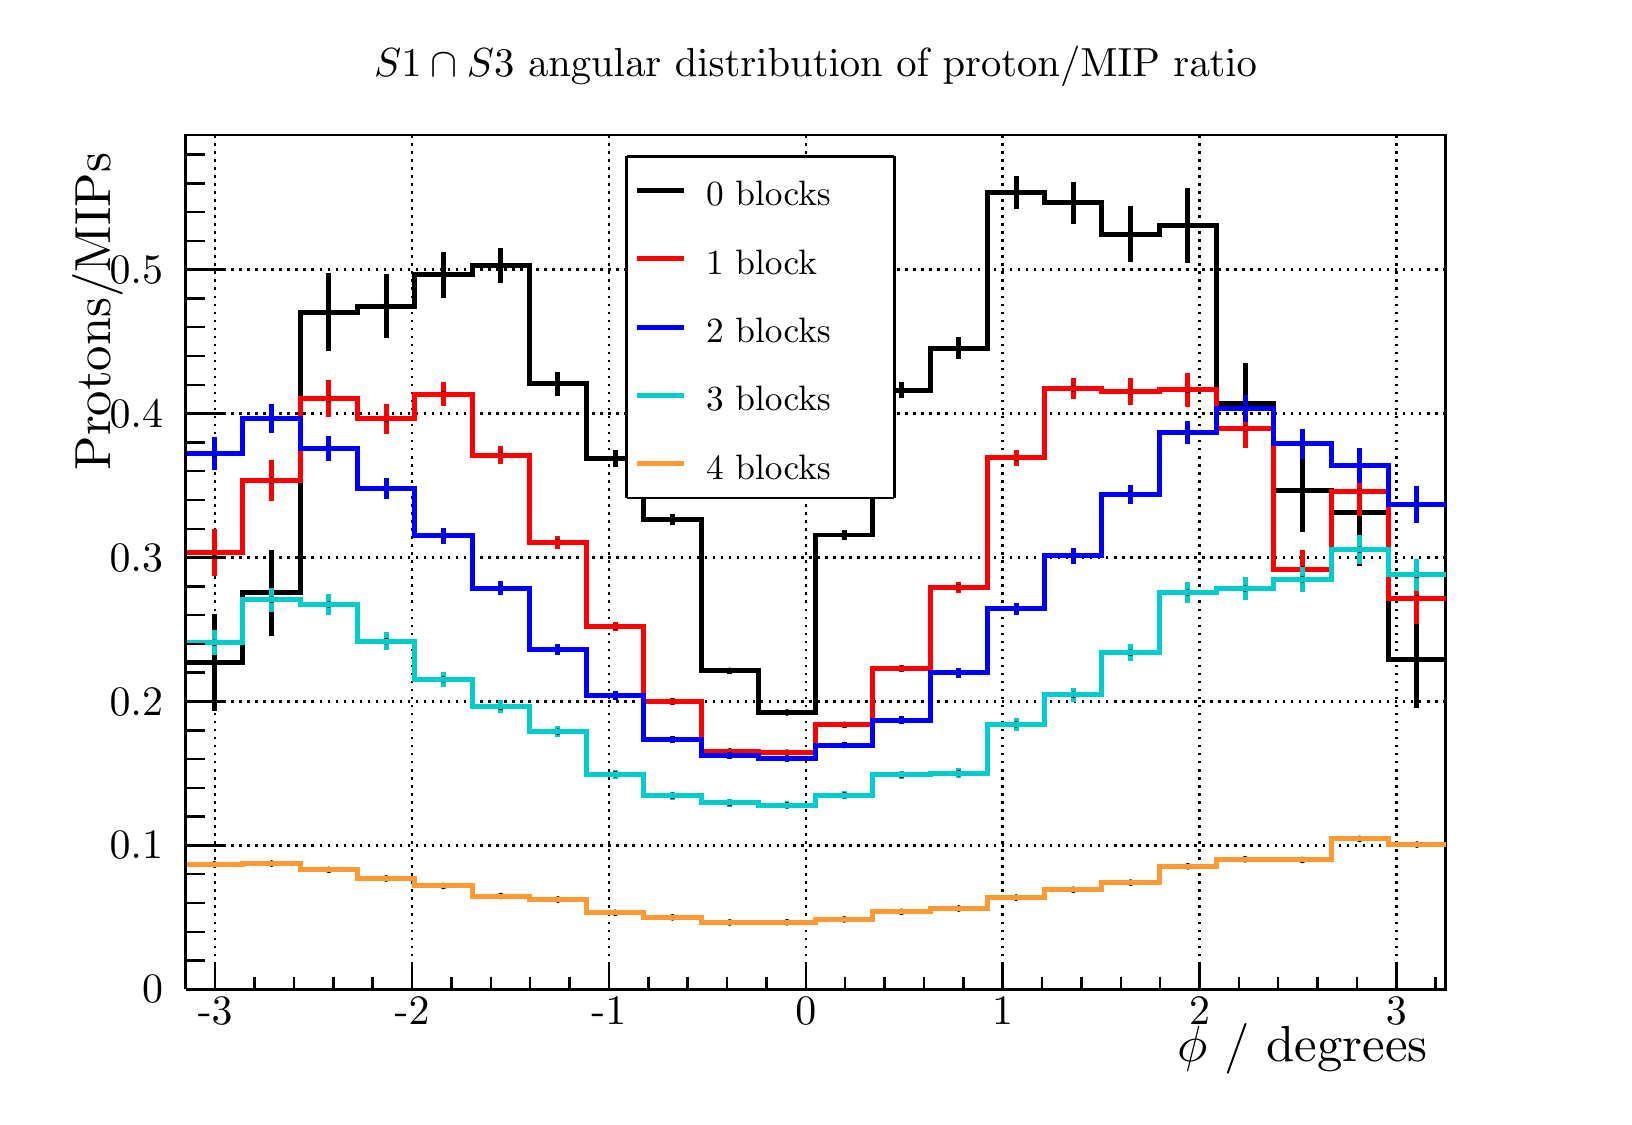
\begin{tikzpicture}
\pgfdeclareplotmark{cross} {
\pgfpathmoveto{\pgfpoint{-0.3\pgfplotmarksize}{\pgfplotmarksize}}
\pgfpathlineto{\pgfpoint{+0.3\pgfplotmarksize}{\pgfplotmarksize}}
\pgfpathlineto{\pgfpoint{+0.3\pgfplotmarksize}{0.3\pgfplotmarksize}}
\pgfpathlineto{\pgfpoint{+1\pgfplotmarksize}{0.3\pgfplotmarksize}}
\pgfpathlineto{\pgfpoint{+1\pgfplotmarksize}{-0.3\pgfplotmarksize}}
\pgfpathlineto{\pgfpoint{+0.3\pgfplotmarksize}{-0.3\pgfplotmarksize}}
\pgfpathlineto{\pgfpoint{+0.3\pgfplotmarksize}{-1.\pgfplotmarksize}}
\pgfpathlineto{\pgfpoint{-0.3\pgfplotmarksize}{-1.\pgfplotmarksize}}
\pgfpathlineto{\pgfpoint{-0.3\pgfplotmarksize}{-0.3\pgfplotmarksize}}
\pgfpathlineto{\pgfpoint{-1.\pgfplotmarksize}{-0.3\pgfplotmarksize}}
\pgfpathlineto{\pgfpoint{-1.\pgfplotmarksize}{0.3\pgfplotmarksize}}
\pgfpathlineto{\pgfpoint{-0.3\pgfplotmarksize}{0.3\pgfplotmarksize}}
\pgfpathclose
\pgfusepathqstroke
}
\pgfdeclareplotmark{cross*} {
\pgfpathmoveto{\pgfpoint{-0.3\pgfplotmarksize}{\pgfplotmarksize}}
\pgfpathlineto{\pgfpoint{+0.3\pgfplotmarksize}{\pgfplotmarksize}}
\pgfpathlineto{\pgfpoint{+0.3\pgfplotmarksize}{0.3\pgfplotmarksize}}
\pgfpathlineto{\pgfpoint{+1\pgfplotmarksize}{0.3\pgfplotmarksize}}
\pgfpathlineto{\pgfpoint{+1\pgfplotmarksize}{-0.3\pgfplotmarksize}}
\pgfpathlineto{\pgfpoint{+0.3\pgfplotmarksize}{-0.3\pgfplotmarksize}}
\pgfpathlineto{\pgfpoint{+0.3\pgfplotmarksize}{-1.\pgfplotmarksize}}
\pgfpathlineto{\pgfpoint{-0.3\pgfplotmarksize}{-1.\pgfplotmarksize}}
\pgfpathlineto{\pgfpoint{-0.3\pgfplotmarksize}{-0.3\pgfplotmarksize}}
\pgfpathlineto{\pgfpoint{-1.\pgfplotmarksize}{-0.3\pgfplotmarksize}}
\pgfpathlineto{\pgfpoint{-1.\pgfplotmarksize}{0.3\pgfplotmarksize}}
\pgfpathlineto{\pgfpoint{-0.3\pgfplotmarksize}{0.3\pgfplotmarksize}}
\pgfpathclose
\pgfusepathqfillstroke
}
\pgfdeclareplotmark{newstar} {
\pgfpathmoveto{\pgfqpoint{0pt}{\pgfplotmarksize}}
\pgfpathlineto{\pgfqpointpolar{44}{0.5\pgfplotmarksize}}
\pgfpathlineto{\pgfqpointpolar{18}{\pgfplotmarksize}}
\pgfpathlineto{\pgfqpointpolar{-20}{0.5\pgfplotmarksize}}
\pgfpathlineto{\pgfqpointpolar{-54}{\pgfplotmarksize}}
\pgfpathlineto{\pgfqpointpolar{-90}{0.5\pgfplotmarksize}}
\pgfpathlineto{\pgfqpointpolar{234}{\pgfplotmarksize}}
\pgfpathlineto{\pgfqpointpolar{198}{0.5\pgfplotmarksize}}
\pgfpathlineto{\pgfqpointpolar{162}{\pgfplotmarksize}}
\pgfpathlineto{\pgfqpointpolar{134}{0.5\pgfplotmarksize}}
\pgfpathclose
\pgfusepathqstroke
}
\pgfdeclareplotmark{newstar*} {
\pgfpathmoveto{\pgfqpoint{0pt}{\pgfplotmarksize}}
\pgfpathlineto{\pgfqpointpolar{44}{0.5\pgfplotmarksize}}
\pgfpathlineto{\pgfqpointpolar{18}{\pgfplotmarksize}}
\pgfpathlineto{\pgfqpointpolar{-20}{0.5\pgfplotmarksize}}
\pgfpathlineto{\pgfqpointpolar{-54}{\pgfplotmarksize}}
\pgfpathlineto{\pgfqpointpolar{-90}{0.5\pgfplotmarksize}}
\pgfpathlineto{\pgfqpointpolar{234}{\pgfplotmarksize}}
\pgfpathlineto{\pgfqpointpolar{198}{0.5\pgfplotmarksize}}
\pgfpathlineto{\pgfqpointpolar{162}{\pgfplotmarksize}}
\pgfpathlineto{\pgfqpointpolar{134}{0.5\pgfplotmarksize}}
\pgfpathclose
\pgfusepathqfillstroke
}
\definecolor{c}{rgb}{1,1,1};
\draw [color=c, fill=c] (0,0) rectangle (20,13.5632);
\draw [color=c, fill=c] (2,1.35632) rectangle (18,12.2069);
\definecolor{c}{rgb}{0,0,0};
\draw [c,line width=0.9] (2,1.35632) -- (2,12.2069) -- (18,12.2069) -- (18,1.35632) -- (2,1.35632);
\definecolor{c}{rgb}{1,1,1};
\draw [color=c, fill=c] (2,1.35632) rectangle (18,12.2069);
\definecolor{c}{rgb}{0,0,0};
\draw [c,line width=0.9] (2,1.35632) -- (2,12.2069) -- (18,12.2069) -- (18,1.35632) -- (2,1.35632);
\draw [c,line width=0.9] (2,1.35632) -- (18,1.35632);
\draw [c,dotted,line width=0.9] (2.375,12.2069) -- (2.375,1.35632);
\draw [c,dotted,line width=0.9] (4.875,12.2069) -- (4.875,1.35632);
\draw [c,dotted,line width=0.9] (7.375,12.2069) -- (7.375,1.35632);
\draw [c,dotted,line width=0.9] (9.875,12.2069) -- (9.875,1.35632);
\draw [c,dotted,line width=0.9] (12.375,12.2069) -- (12.375,1.35632);
\draw [c,dotted,line width=0.9] (14.875,12.2069) -- (14.875,1.35632);
\draw [c,dotted,line width=0.9] (17.375,12.2069) -- (17.375,1.35632);
\draw [c,dotted,line width=0.9] (2.375,12.2069) -- (2.375,1.35632);
\draw [c,dotted,line width=0.9] (17.375,12.2069) -- (17.375,1.35632);
\draw [c,line width=0.9] (2,1.35632) -- (2,12.2069);
\draw [c,dotted,line width=0.9] (18,1.35632) -- (2,1.35632);
\draw [c,dotted,line width=0.9] (18,3.18443) -- (2,3.18443);
\draw [c,dotted,line width=0.9] (18,5.01255) -- (2,5.01255);
\draw [c,dotted,line width=0.9] (18,6.84066) -- (2,6.84066);
\draw [c,dotted,line width=0.9] (18,8.66877) -- (2,8.66877);
\draw [c,dotted,line width=0.9] (18,10.4969) -- (2,10.4969);
\draw [c,dotted,line width=0.9] (18,10.4969) -- (2,10.4969);
\definecolor{c}{rgb}{0,0,0.6};
\draw [c,line width=0.9] (2,1.35632) -- (2.72727,1.35632) -- (2.72727,1.35632) -- (3.45455,1.35632) -- (3.45455,1.35632) -- (4.18182,1.35632) -- (4.18182,1.35632) -- (4.90909,1.35632) -- (4.90909,1.35632) -- (5.63636,1.35632) -- (5.63636,1.35632) --
 (6.36364,1.35632) -- (6.36364,1.35632) -- (7.09091,1.35632) -- (7.09091,1.35632) -- (7.81818,1.35632) -- (7.81818,1.35632) -- (8.54545,1.35632) -- (8.54545,1.35632) -- (9.27273,1.35632) -- (9.27273,1.35632) -- (10,1.35632) -- (10,1.35632) --
 (10.7273,1.35632) -- (10.7273,1.35632) -- (11.4545,1.35632) -- (11.4545,1.35632) -- (12.1818,1.35632) -- (12.1818,1.35632) -- (12.9091,1.35632) -- (12.9091,1.35632) -- (13.6364,1.35632) -- (13.6364,1.35632) -- (14.3636,1.35632) -- (14.3636,1.35632)
 -- (15.0909,1.35632) -- (15.0909,1.35632) -- (15.8182,1.35632) -- (15.8182,1.35632) -- (16.5455,1.35632) -- (16.5455,1.35632) -- (17.2727,1.35632) -- (17.2727,1.35632) -- (18,1.35632);
\definecolor{c}{rgb}{0,0,0};
\draw [c,line width=0.9] (2,1.35632) -- (18,1.35632);
\draw [anchor= east] (18,0.596782) node[scale=1.8317, color=c, rotate=0]{$\phi$ / degrees};
\draw [c,line width=0.9] (2.375,1.68184) -- (2.375,1.35632);
\draw [c,line width=0.9] (2.875,1.51908) -- (2.875,1.35632);
\draw [c,line width=0.9] (3.375,1.51908) -- (3.375,1.35632);
\draw [c,line width=0.9] (3.875,1.51908) -- (3.875,1.35632);
\draw [c,line width=0.9] (4.375,1.51908) -- (4.375,1.35632);
\draw [c,line width=0.9] (4.875,1.68184) -- (4.875,1.35632);
\draw [c,line width=0.9] (5.375,1.51908) -- (5.375,1.35632);
\draw [c,line width=0.9] (5.875,1.51908) -- (5.875,1.35632);
\draw [c,line width=0.9] (6.375,1.51908) -- (6.375,1.35632);
\draw [c,line width=0.9] (6.875,1.51908) -- (6.875,1.35632);
\draw [c,line width=0.9] (7.375,1.68184) -- (7.375,1.35632);
\draw [c,line width=0.9] (7.875,1.51908) -- (7.875,1.35632);
\draw [c,line width=0.9] (8.375,1.51908) -- (8.375,1.35632);
\draw [c,line width=0.9] (8.875,1.51908) -- (8.875,1.35632);
\draw [c,line width=0.9] (9.375,1.51908) -- (9.375,1.35632);
\draw [c,line width=0.9] (9.875,1.68184) -- (9.875,1.35632);
\draw [c,line width=0.9] (10.375,1.51908) -- (10.375,1.35632);
\draw [c,line width=0.9] (10.875,1.51908) -- (10.875,1.35632);
\draw [c,line width=0.9] (11.375,1.51908) -- (11.375,1.35632);
\draw [c,line width=0.9] (11.875,1.51908) -- (11.875,1.35632);
\draw [c,line width=0.9] (12.375,1.68184) -- (12.375,1.35632);
\draw [c,line width=0.9] (12.875,1.51908) -- (12.875,1.35632);
\draw [c,line width=0.9] (13.375,1.51908) -- (13.375,1.35632);
\draw [c,line width=0.9] (13.875,1.51908) -- (13.875,1.35632);
\draw [c,line width=0.9] (14.375,1.51908) -- (14.375,1.35632);
\draw [c,line width=0.9] (14.875,1.68184) -- (14.875,1.35632);
\draw [c,line width=0.9] (15.375,1.51908) -- (15.375,1.35632);
\draw [c,line width=0.9] (15.875,1.51908) -- (15.875,1.35632);
\draw [c,line width=0.9] (16.375,1.51908) -- (16.375,1.35632);
\draw [c,line width=0.9] (16.875,1.51908) -- (16.875,1.35632);
\draw [c,line width=0.9] (17.375,1.68184) -- (17.375,1.35632);
\draw [c,line width=0.9] (2.375,1.68184) -- (2.375,1.35632);
\draw [c,line width=0.9] (17.375,1.68184) -- (17.375,1.35632);
\draw [c,line width=0.9] (17.875,1.51908) -- (17.875,1.35632);
\draw [anchor=base] (2.375,0.908736) node[scale=1.5137, color=c, rotate=0]{-3};
\draw [anchor=base] (4.875,0.908736) node[scale=1.5137, color=c, rotate=0]{-2};
\draw [anchor=base] (7.375,0.908736) node[scale=1.5137, color=c, rotate=0]{-1};
\draw [anchor=base] (9.875,0.908736) node[scale=1.5137, color=c, rotate=0]{0};
\draw [anchor=base] (12.375,0.908736) node[scale=1.5137, color=c, rotate=0]{1};
\draw [anchor=base] (14.875,0.908736) node[scale=1.5137, color=c, rotate=0]{2};
\draw [anchor=base] (17.375,0.908736) node[scale=1.5137, color=c, rotate=0]{3};
\draw [c,line width=0.9] (2,1.35632) -- (2,12.2069);
\draw [anchor= east] (0.88,12.2069) node[scale=1.8317, color=c, rotate=90]{  Protons/MIPs};
\draw [c,line width=0.9] (2.48,1.35632) -- (2,1.35632);
\draw [c,line width=0.9] (2.24,1.72194) -- (2,1.72194);
\draw [c,line width=0.9] (2.24,2.08757) -- (2,2.08757);
\draw [c,line width=0.9] (2.24,2.45319) -- (2,2.45319);
\draw [c,line width=0.9] (2.24,2.81881) -- (2,2.81881);
\draw [c,line width=0.9] (2.48,3.18443) -- (2,3.18443);
\draw [c,line width=0.9] (2.24,3.55006) -- (2,3.55006);
\draw [c,line width=0.9] (2.24,3.91568) -- (2,3.91568);
\draw [c,line width=0.9] (2.24,4.2813) -- (2,4.2813);
\draw [c,line width=0.9] (2.24,4.64692) -- (2,4.64692);
\draw [c,line width=0.9] (2.48,5.01255) -- (2,5.01255);
\draw [c,line width=0.9] (2.24,5.37817) -- (2,5.37817);
\draw [c,line width=0.9] (2.24,5.74379) -- (2,5.74379);
\draw [c,line width=0.9] (2.24,6.10941) -- (2,6.10941);
\draw [c,line width=0.9] (2.24,6.47504) -- (2,6.47504);
\draw [c,line width=0.9] (2.48,6.84066) -- (2,6.84066);
\draw [c,line width=0.9] (2.24,7.20628) -- (2,7.20628);
\draw [c,line width=0.9] (2.24,7.5719) -- (2,7.5719);
\draw [c,line width=0.9] (2.24,7.93753) -- (2,7.93753);
\draw [c,line width=0.9] (2.24,8.30315) -- (2,8.30315);
\draw [c,line width=0.9] (2.48,8.66877) -- (2,8.66877);
\draw [c,line width=0.9] (2.24,9.03439) -- (2,9.03439);
\draw [c,line width=0.9] (2.24,9.40002) -- (2,9.40002);
\draw [c,line width=0.9] (2.24,9.76564) -- (2,9.76564);
\draw [c,line width=0.9] (2.24,10.1313) -- (2,10.1313);
\draw [c,line width=0.9] (2.48,10.4969) -- (2,10.4969);
\draw [c,line width=0.9] (2.48,10.4969) -- (2,10.4969);
\draw [c,line width=0.9] (2.24,10.8625) -- (2,10.8625);
\draw [c,line width=0.9] (2.24,11.2281) -- (2,11.2281);
\draw [c,line width=0.9] (2.24,11.5938) -- (2,11.5938);
\draw [c,line width=0.9] (2.24,11.9594) -- (2,11.9594);
\draw [anchor= east] (1.9,1.35632) node[scale=1.5137, color=c, rotate=0]{0};
\draw [anchor= east] (1.9,3.18443) node[scale=1.5137, color=c, rotate=0]{0.1};
\draw [anchor= east] (1.9,5.01255) node[scale=1.5137, color=c, rotate=0]{0.2};
\draw [anchor= east] (1.9,6.84066) node[scale=1.5137, color=c, rotate=0]{0.3};
\draw [anchor= east] (1.9,8.66877) node[scale=1.5137, color=c, rotate=0]{0.4};
\draw [anchor= east] (1.9,10.4969) node[scale=1.5137, color=c, rotate=0]{0.5};
\draw [c,line width=1.8] (2.36364,4.89378) -- (2.36364,5.51112);
\draw [c,line width=1.8] (2.36364,5.51112) -- (2.36364,6.12847);
\foreach \P in {(2.36364,5.51112)}{\draw[mark options={color=c,fill=c},mark size=2.402402pt,mark=*,mark size=1pt] plot coordinates {\P};}
\draw [c,line width=1.8] (3.09091,5.84926) -- (3.09091,6.39379);
\draw [c,line width=1.8] (3.09091,6.39379) -- (3.09091,6.93831);
\foreach \P in {(3.09091,6.39379)}{\draw[mark options={color=c,fill=c},mark size=2.402402pt,mark=*,mark size=1pt] plot coordinates {\P};}
\draw [c,line width=1.8] (3.81818,9.45971) -- (3.81818,9.95602);
\draw [c,line width=1.8] (3.81818,9.95602) -- (3.81818,10.4523);
\foreach \P in {(3.81818,9.95602)}{\draw[mark options={color=c,fill=c},mark size=2.402402pt,mark=*,mark size=1pt] plot coordinates {\P};}
\draw [c,line width=1.8] (4.54545,9.62928) -- (4.54545,10.0327);
\draw [c,line width=1.8] (4.54545,10.0327) -- (4.54545,10.4362);
\foreach \P in {(4.54545,10.0327)}{\draw[mark options={color=c,fill=c},mark size=2.402402pt,mark=*,mark size=1pt] plot coordinates {\P};}
\draw [c,line width=1.8] (5.27273,10.1359) -- (5.27273,10.4304);
\draw [c,line width=1.8] (5.27273,10.4304) -- (5.27273,10.725);
\foreach \P in {(5.27273,10.4304)}{\draw[mark options={color=c,fill=c},mark size=2.402402pt,mark=*,mark size=1pt] plot coordinates {\P};}
\draw [c,line width=1.8] (6,10.3215) -- (6,10.547);
\draw [c,line width=1.8] (6,10.547) -- (6,10.7725);
\foreach \P in {(6,10.547)}{\draw[mark options={color=c,fill=c},mark size=2.402402pt,mark=*,mark size=1pt] plot coordinates {\P};}
\draw [c,line width=1.8] (6.72727,8.89213) -- (6.72727,9.04764);
\draw [c,line width=1.8] (6.72727,9.04764) -- (6.72727,9.20315);
\foreach \P in {(6.72727,9.04764)}{\draw[mark options={color=c,fill=c},mark size=2.402402pt,mark=*,mark size=1pt] plot coordinates {\P};}
\draw [c,line width=1.8] (7.45455,7.99309) -- (7.45455,8.09945);
\draw [c,line width=1.8] (7.45455,8.09945) -- (7.45455,8.2058);
\foreach \P in {(7.45455,8.09945)}{\draw[mark options={color=c,fill=c},mark size=2.402402pt,mark=*,mark size=1pt] plot coordinates {\P};}
\draw [c,line width=1.8] (8.18182,7.25752) -- (8.18182,7.3273);
\draw [c,line width=1.8] (8.18182,7.3273) -- (8.18182,7.39708);
\foreach \P in {(8.18182,7.3273)}{\draw[mark options={color=c,fill=c},mark size=2.402402pt,mark=*,mark size=1pt] plot coordinates {\P};}
\draw [c,line width=1.8] (8.90909,5.36598) -- (8.90909,5.40179);
\draw [c,line width=1.8] (8.90909,5.40179) -- (8.90909,5.4376);
\foreach \P in {(8.90909,5.40179)}{\draw[mark options={color=c,fill=c},mark size=2.402402pt,mark=*,mark size=1pt] plot coordinates {\P};}
\draw [c,line width=1.8] (9.63636,4.84341) -- (9.63636,4.87303);
\draw [c,line width=1.8] (9.63636,4.87303) -- (9.63636,4.90264);
\foreach \P in {(9.63636,4.87303)}{\draw[mark options={color=c,fill=c},mark size=2.402402pt,mark=*,mark size=1pt] plot coordinates {\P};}
\draw [c,line width=1.8] (10.3636,7.06938) -- (10.3636,7.12713);
\draw [c,line width=1.8] (10.3636,7.12713) -- (10.3636,7.18488);
\foreach \P in {(10.3636,7.12713)}{\draw[mark options={color=c,fill=c},mark size=2.402402pt,mark=*,mark size=1pt] plot coordinates {\P};}
\draw [c,line width=1.8] (11.0909,8.86292) -- (11.0909,8.96454);
\draw [c,line width=1.8] (11.0909,8.96454) -- (11.0909,9.06617);
\foreach \P in {(11.0909,8.96454)}{\draw[mark options={color=c,fill=c},mark size=2.402402pt,mark=*,mark size=1pt] plot coordinates {\P};}
\draw [c,line width=1.8] (11.8182,9.36011) -- (11.8182,9.50073);
\draw [c,line width=1.8] (11.8182,9.50073) -- (11.8182,9.64135);
\foreach \P in {(11.8182,9.50073)}{\draw[mark options={color=c,fill=c},mark size=2.402402pt,mark=*,mark size=1pt] plot coordinates {\P};}
\draw [c,line width=1.8] (12.5455,11.263) -- (12.5455,11.4766);
\draw [c,line width=1.8] (12.5455,11.4766) -- (12.5455,11.6902);
\foreach \P in {(12.5455,11.4766)}{\draw[mark options={color=c,fill=c},mark size=2.402402pt,mark=*,mark size=1pt] plot coordinates {\P};}
\draw [c,line width=1.8] (13.2727,11.0759) -- (13.2727,11.3437);
\draw [c,line width=1.8] (13.2727,11.3437) -- (13.2727,11.6115);
\foreach \P in {(13.2727,11.3437)}{\draw[mark options={color=c,fill=c},mark size=2.402402pt,mark=*,mark size=1pt] plot coordinates {\P};}
\draw [c,line width=1.8] (14,10.588) -- (14,10.9455);
\draw [c,line width=1.8] (14,10.9455) -- (14,11.303);
\foreach \P in {(14,10.9455)}{\draw[mark options={color=c,fill=c},mark size=2.402402pt,mark=*,mark size=1pt] plot coordinates {\P};}
\draw [c,line width=1.8] (14.7273,10.5864) -- (14.7273,11.0575);
\draw [c,line width=1.8] (14.7273,11.0575) -- (14.7273,11.5286);
\foreach \P in {(14.7273,11.0575)}{\draw[mark options={color=c,fill=c},mark size=2.402402pt,mark=*,mark size=1pt] plot coordinates {\P};}
\draw [c,line width=1.8] (15.4545,8.28922) -- (15.4545,8.79768);
\draw [c,line width=1.8] (15.4545,8.79768) -- (15.4545,9.30614);
\foreach \P in {(15.4545,8.79768)}{\draw[mark options={color=c,fill=c},mark size=2.402402pt,mark=*,mark size=1pt] plot coordinates {\P};}
\draw [c,line width=1.8] (16.1818,7.16906) -- (16.1818,7.69467);
\draw [c,line width=1.8] (16.1818,7.69467) -- (16.1818,8.22028);
\foreach \P in {(16.1818,7.69467)}{\draw[mark options={color=c,fill=c},mark size=2.402402pt,mark=*,mark size=1pt] plot coordinates {\P};}
\draw [c,line width=1.8] (16.9091,6.73172) -- (16.9091,7.41194);
\draw [c,line width=1.8] (16.9091,7.41194) -- (16.9091,8.09217);
\foreach \P in {(16.9091,7.41194)}{\draw[mark options={color=c,fill=c},mark size=2.402402pt,mark=*,mark size=1pt] plot coordinates {\P};}
\draw [c,line width=1.8] (17.6364,4.93484) -- (17.6364,5.54817);
\draw [c,line width=1.8] (17.6364,5.54817) -- (17.6364,6.16151);
\foreach \P in {(17.6364,5.54817)}{\draw[mark options={color=c,fill=c},mark size=2.402402pt,mark=*,mark size=1pt] plot coordinates {\P};}
\draw [c,line width=1.8] (2,5.51112) -- (2.72727,5.51112) -- (2.72727,6.39379) -- (3.45455,6.39379) -- (3.45455,9.95602) -- (4.18182,9.95602) -- (4.18182,10.0327) -- (4.90909,10.0327) -- (4.90909,10.4304) -- (5.63636,10.4304) -- (5.63636,10.547) --
 (6.36364,10.547) -- (6.36364,9.04764) -- (7.09091,9.04764) -- (7.09091,8.09945) -- (7.81818,8.09945) -- (7.81818,7.3273) -- (8.54545,7.3273) -- (8.54545,5.40179) -- (9.27273,5.40179) -- (9.27273,4.87303) -- (10,4.87303) -- (10,7.12713) --
 (10.7273,7.12713) -- (10.7273,8.96454) -- (11.4545,8.96454) -- (11.4545,9.50073) -- (12.1818,9.50073) -- (12.1818,11.4766) -- (12.9091,11.4766) -- (12.9091,11.3437) -- (13.6364,11.3437) -- (13.6364,10.9455) -- (14.3636,10.9455) -- (14.3636,11.0575)
 -- (15.0909,11.0575) -- (15.0909,8.79768) -- (15.8182,8.79768) -- (15.8182,7.69467) -- (16.5455,7.69467) -- (16.5455,7.41194) -- (17.2727,7.41194) -- (17.2727,5.54817) -- (18,5.54817);
\definecolor{c}{rgb}{1,0,0};
\draw [c,line width=1.8] (2.36364,6.60423) -- (2.36364,6.90306);
\draw [c,line width=1.8] (2.36364,6.90306) -- (2.36364,7.20189);
\definecolor{c}{rgb}{0,0,0};
\foreach \P in {(2.36364,6.90306)}{\draw[mark options={color=c,fill=c},mark size=2.402402pt,mark=*,mark size=1pt] plot coordinates {\P};}
\definecolor{c}{rgb}{1,0,0};
\draw [c,line width=1.8] (3.09091,7.5545) -- (3.09091,7.8162);
\draw [c,line width=1.8] (3.09091,7.8162) -- (3.09091,8.0779);
\definecolor{c}{rgb}{0,0,0};
\foreach \P in {(3.09091,7.8162)}{\draw[mark options={color=c,fill=c},mark size=2.402402pt,mark=*,mark size=1pt] plot coordinates {\P};}
\definecolor{c}{rgb}{1,0,0};
\draw [c,line width=1.8] (3.81818,8.62873) -- (3.81818,8.86031);
\draw [c,line width=1.8] (3.81818,8.86031) -- (3.81818,9.09189);
\definecolor{c}{rgb}{0,0,0};
\foreach \P in {(3.81818,8.86031)}{\draw[mark options={color=c,fill=c},mark size=2.402402pt,mark=*,mark size=1pt] plot coordinates {\P};}
\definecolor{c}{rgb}{1,0,0};
\draw [c,line width=1.8] (4.54545,8.41495) -- (4.54545,8.60083);
\draw [c,line width=1.8] (4.54545,8.60083) -- (4.54545,8.78671);
\definecolor{c}{rgb}{0,0,0};
\foreach \P in {(4.54545,8.60083)}{\draw[mark options={color=c,fill=c},mark size=2.402402pt,mark=*,mark size=1pt] plot coordinates {\P};}
\definecolor{c}{rgb}{1,0,0};
\draw [c,line width=1.8] (5.27273,8.76828) -- (5.27273,8.91648);
\draw [c,line width=1.8] (5.27273,8.91648) -- (5.27273,9.06469);
\definecolor{c}{rgb}{0,0,0};
\foreach \P in {(5.27273,8.91648)}{\draw[mark options={color=c,fill=c},mark size=2.402402pt,mark=*,mark size=1pt] plot coordinates {\P};}
\definecolor{c}{rgb}{1,0,0};
\draw [c,line width=1.8] (6,8.02779) -- (6,8.14192);
\draw [c,line width=1.8] (6,8.14192) -- (6,8.25604);
\definecolor{c}{rgb}{0,0,0};
\foreach \P in {(6,8.14192)}{\draw[mark options={color=c,fill=c},mark size=2.402402pt,mark=*,mark size=1pt] plot coordinates {\P};}
\definecolor{c}{rgb}{1,0,0};
\draw [c,line width=1.8] (6.72727,6.95442) -- (6.72727,7.03619);
\draw [c,line width=1.8] (6.72727,7.03619) -- (6.72727,7.11796);
\definecolor{c}{rgb}{0,0,0};
\foreach \P in {(6.72727,7.03619)}{\draw[mark options={color=c,fill=c},mark size=2.402402pt,mark=*,mark size=1pt] plot coordinates {\P};}
\definecolor{c}{rgb}{1,0,0};
\draw [c,line width=1.8] (7.45455,5.90288) -- (7.45455,5.96141);
\draw [c,line width=1.8] (7.45455,5.96141) -- (7.45455,6.01994);
\definecolor{c}{rgb}{0,0,0};
\foreach \P in {(7.45455,5.96141)}{\draw[mark options={color=c,fill=c},mark size=2.402402pt,mark=*,mark size=1pt] plot coordinates {\P};}
\definecolor{c}{rgb}{1,0,0};
\draw [c,line width=1.8] (8.18182,4.97126) -- (8.18182,5.01446);
\draw [c,line width=1.8] (8.18182,5.01446) -- (8.18182,5.05766);
\definecolor{c}{rgb}{0,0,0};
\foreach \P in {(8.18182,5.01446)}{\draw[mark options={color=c,fill=c},mark size=2.402402pt,mark=*,mark size=1pt] plot coordinates {\P};}
\definecolor{c}{rgb}{1,0,0};
\draw [c,line width=1.8] (8.90909,4.34427) -- (8.90909,4.37898);
\draw [c,line width=1.8] (8.90909,4.37898) -- (8.90909,4.41369);
\definecolor{c}{rgb}{0,0,0};
\foreach \P in {(8.90909,4.37898)}{\draw[mark options={color=c,fill=c},mark size=2.402402pt,mark=*,mark size=1pt] plot coordinates {\P};}
\definecolor{c}{rgb}{1,0,0};
\draw [c,line width=1.8] (9.63636,4.32923) -- (9.63636,4.3633);
\draw [c,line width=1.8] (9.63636,4.3633) -- (9.63636,4.39736);
\definecolor{c}{rgb}{0,0,0};
\foreach \P in {(9.63636,4.3633)}{\draw[mark options={color=c,fill=c},mark size=2.402402pt,mark=*,mark size=1pt] plot coordinates {\P};}
\definecolor{c}{rgb}{1,0,0};
\draw [c,line width=1.8] (10.3636,4.67726) -- (10.3636,4.71602);
\draw [c,line width=1.8] (10.3636,4.71602) -- (10.3636,4.75479);
\definecolor{c}{rgb}{0,0,0};
\foreach \P in {(10.3636,4.71602)}{\draw[mark options={color=c,fill=c},mark size=2.402402pt,mark=*,mark size=1pt] plot coordinates {\P};}
\definecolor{c}{rgb}{1,0,0};
\draw [c,line width=1.8] (11.0909,5.38166) -- (11.0909,5.43154);
\draw [c,line width=1.8] (11.0909,5.43154) -- (11.0909,5.48143);
\definecolor{c}{rgb}{0,0,0};
\foreach \P in {(11.0909,5.43154)}{\draw[mark options={color=c,fill=c},mark size=2.402402pt,mark=*,mark size=1pt] plot coordinates {\P};}
\definecolor{c}{rgb}{1,0,0};
\draw [c,line width=1.8] (11.8182,6.39514) -- (11.8182,6.46287);
\draw [c,line width=1.8] (11.8182,6.46287) -- (11.8182,6.5306);
\definecolor{c}{rgb}{0,0,0};
\foreach \P in {(11.8182,6.46287)}{\draw[mark options={color=c,fill=c},mark size=2.402402pt,mark=*,mark size=1pt] plot coordinates {\P};}
\definecolor{c}{rgb}{1,0,0};
\draw [c,line width=1.8] (12.5455,8.00437) -- (12.5455,8.10677);
\draw [c,line width=1.8] (12.5455,8.10677) -- (12.5455,8.20917);
\definecolor{c}{rgb}{0,0,0};
\foreach \P in {(12.5455,8.10677)}{\draw[mark options={color=c,fill=c},mark size=2.402402pt,mark=*,mark size=1pt] plot coordinates {\P};}
\definecolor{c}{rgb}{1,0,0};
\draw [c,line width=1.8] (13.2727,8.85335) -- (13.2727,8.98853);
\draw [c,line width=1.8] (13.2727,8.98853) -- (13.2727,9.1237);
\definecolor{c}{rgb}{0,0,0};
\foreach \P in {(13.2727,8.98853)}{\draw[mark options={color=c,fill=c},mark size=2.402402pt,mark=*,mark size=1pt] plot coordinates {\P};}
\definecolor{c}{rgb}{1,0,0};
\draw [c,line width=1.8] (14,8.77802) -- (14,8.94714);
\draw [c,line width=1.8] (14,8.94714) -- (14,9.11627);
\definecolor{c}{rgb}{0,0,0};
\foreach \P in {(14,8.94714)}{\draw[mark options={color=c,fill=c},mark size=2.402402pt,mark=*,mark size=1pt] plot coordinates {\P};}
\definecolor{c}{rgb}{1,0,0};
\draw [c,line width=1.8] (14.7273,8.75518) -- (14.7273,8.96999);
\draw [c,line width=1.8] (14.7273,8.96999) -- (14.7273,9.18481);
\definecolor{c}{rgb}{0,0,0};
\foreach \P in {(14.7273,8.96999)}{\draw[mark options={color=c,fill=c},mark size=2.402402pt,mark=*,mark size=1pt] plot coordinates {\P};}
\definecolor{c}{rgb}{1,0,0};
\draw [c,line width=1.8] (15.4545,8.23655) -- (15.4545,8.47919);
\draw [c,line width=1.8] (15.4545,8.47919) -- (15.4545,8.72183);
\definecolor{c}{rgb}{0,0,0};
\foreach \P in {(15.4545,8.47919)}{\draw[mark options={color=c,fill=c},mark size=2.402402pt,mark=*,mark size=1pt] plot coordinates {\P};}
\definecolor{c}{rgb}{1,0,0};
\draw [c,line width=1.8] (16.1818,6.44051) -- (16.1818,6.69109);
\draw [c,line width=1.8] (16.1818,6.69109) -- (16.1818,6.94166);
\definecolor{c}{rgb}{0,0,0};
\foreach \P in {(16.1818,6.69109)}{\draw[mark options={color=c,fill=c},mark size=2.402402pt,mark=*,mark size=1pt] plot coordinates {\P};}
\definecolor{c}{rgb}{1,0,0};
\draw [c,line width=1.8] (16.9091,7.36681) -- (16.9091,7.68164);
\draw [c,line width=1.8] (16.9091,7.68164) -- (16.9091,7.99646);
\definecolor{c}{rgb}{0,0,0};
\foreach \P in {(16.9091,7.68164)}{\draw[mark options={color=c,fill=c},mark size=2.402402pt,mark=*,mark size=1pt] plot coordinates {\P};}
\definecolor{c}{rgb}{1,0,0};
\draw [c,line width=1.8] (17.6364,5.99877) -- (17.6364,6.32595);
\draw [c,line width=1.8] (17.6364,6.32595) -- (17.6364,6.65312);
\definecolor{c}{rgb}{0,0,0};
\foreach \P in {(17.6364,6.32595)}{\draw[mark options={color=c,fill=c},mark size=2.402402pt,mark=*,mark size=1pt] plot coordinates {\P};}
\definecolor{c}{rgb}{1,0,0};
\draw [c,line width=1.8] (2,6.90306) -- (2.72727,6.90306) -- (2.72727,7.8162) -- (3.45455,7.8162) -- (3.45455,8.86031) -- (4.18182,8.86031) -- (4.18182,8.60083) -- (4.90909,8.60083) -- (4.90909,8.91648) -- (5.63636,8.91648) -- (5.63636,8.14192) --
 (6.36364,8.14192) -- (6.36364,7.03619) -- (7.09091,7.03619) -- (7.09091,5.96141) -- (7.81818,5.96141) -- (7.81818,5.01446) -- (8.54545,5.01446) -- (8.54545,4.37898) -- (9.27273,4.37898) -- (9.27273,4.3633) -- (10,4.3633) -- (10,4.71602) --
 (10.7273,4.71602) -- (10.7273,5.43154) -- (11.4545,5.43154) -- (11.4545,6.46287) -- (12.1818,6.46287) -- (12.1818,8.10677) -- (12.9091,8.10677) -- (12.9091,8.98853) -- (13.6364,8.98853) -- (13.6364,8.94714) -- (14.3636,8.94714) -- (14.3636,8.96999)
 -- (15.0909,8.96999) -- (15.0909,8.47919) -- (15.8182,8.47919) -- (15.8182,6.69109) -- (16.5455,6.69109) -- (16.5455,7.68164) -- (17.2727,7.68164) -- (17.2727,6.32595) -- (18,6.32595);
\definecolor{c}{rgb}{0,0,1};
\draw [c,line width=1.8] (2.36364,7.94927) -- (2.36364,8.15813);
\draw [c,line width=1.8] (2.36364,8.15813) -- (2.36364,8.36698);
\definecolor{c}{rgb}{0,0,0};
\foreach \P in {(2.36364,8.15813)}{\draw[mark options={color=c,fill=c},mark size=2.402402pt,mark=*,mark size=1pt] plot coordinates {\P};}
\definecolor{c}{rgb}{0,0,1};
\draw [c,line width=1.8] (3.09091,8.41768) -- (3.09091,8.60289);
\draw [c,line width=1.8] (3.09091,8.60289) -- (3.09091,8.78811);
\definecolor{c}{rgb}{0,0,0};
\foreach \P in {(3.09091,8.60289)}{\draw[mark options={color=c,fill=c},mark size=2.402402pt,mark=*,mark size=1pt] plot coordinates {\P};}
\definecolor{c}{rgb}{0,0,1};
\draw [c,line width=1.8] (3.81818,8.07214) -- (3.81818,8.23082);
\draw [c,line width=1.8] (3.81818,8.23082) -- (3.81818,8.38951);
\definecolor{c}{rgb}{0,0,0};
\foreach \P in {(3.81818,8.23082)}{\draw[mark options={color=c,fill=c},mark size=2.402402pt,mark=*,mark size=1pt] plot coordinates {\P};}
\definecolor{c}{rgb}{0,0,1};
\draw [c,line width=1.8] (4.54545,7.58374) -- (4.54545,7.71608);
\draw [c,line width=1.8] (4.54545,7.71608) -- (4.54545,7.84841);
\definecolor{c}{rgb}{0,0,0};
\foreach \P in {(4.54545,7.71608)}{\draw[mark options={color=c,fill=c},mark size=2.402402pt,mark=*,mark size=1pt] plot coordinates {\P};}
\definecolor{c}{rgb}{0,0,1};
\draw [c,line width=1.8] (5.27273,7.0098) -- (5.27273,7.11593);
\draw [c,line width=1.8] (5.27273,7.11593) -- (5.27273,7.22207);
\definecolor{c}{rgb}{0,0,0};
\foreach \P in {(5.27273,7.11593)}{\draw[mark options={color=c,fill=c},mark size=2.402402pt,mark=*,mark size=1pt] plot coordinates {\P};}
\definecolor{c}{rgb}{0,0,1};
\draw [c,line width=1.8] (6,6.36486) -- (6,6.45215);
\draw [c,line width=1.8] (6,6.45215) -- (6,6.53944);
\definecolor{c}{rgb}{0,0,0};
\foreach \P in {(6,6.45215)}{\draw[mark options={color=c,fill=c},mark size=2.402402pt,mark=*,mark size=1pt] plot coordinates {\P};}
\definecolor{c}{rgb}{0,0,1};
\draw [c,line width=1.8] (6.72727,5.60459) -- (6.72727,5.67248);
\draw [c,line width=1.8] (6.72727,5.67248) -- (6.72727,5.74038);
\definecolor{c}{rgb}{0,0,0};
\foreach \P in {(6.72727,5.67248)}{\draw[mark options={color=c,fill=c},mark size=2.402402pt,mark=*,mark size=1pt] plot coordinates {\P};}
\definecolor{c}{rgb}{0,0,1};
\draw [c,line width=1.8] (7.45455,5.03204) -- (7.45455,5.08687);
\draw [c,line width=1.8] (7.45455,5.08687) -- (7.45455,5.14171);
\definecolor{c}{rgb}{0,0,0};
\foreach \P in {(7.45455,5.08687)}{\draw[mark options={color=c,fill=c},mark size=2.402402pt,mark=*,mark size=1pt] plot coordinates {\P};}
\definecolor{c}{rgb}{0,0,1};
\draw [c,line width=1.8] (8.18182,4.4863) -- (8.18182,4.53181);
\draw [c,line width=1.8] (8.18182,4.53181) -- (8.18182,4.57731);
\definecolor{c}{rgb}{0,0,0};
\foreach \P in {(8.18182,4.53181)}{\draw[mark options={color=c,fill=c},mark size=2.402402pt,mark=*,mark size=1pt] plot coordinates {\P};}
\definecolor{c}{rgb}{0,0,1};
\draw [c,line width=1.8] (8.90909,4.287) -- (8.90909,4.32814);
\draw [c,line width=1.8] (8.90909,4.32814) -- (8.90909,4.36928);
\definecolor{c}{rgb}{0,0,0};
\foreach \P in {(8.90909,4.32814)}{\draw[mark options={color=c,fill=c},mark size=2.402402pt,mark=*,mark size=1pt] plot coordinates {\P};}
\definecolor{c}{rgb}{0,0,1};
\draw [c,line width=1.8] (9.63636,4.24632) -- (9.63636,4.28747);
\draw [c,line width=1.8] (9.63636,4.28747) -- (9.63636,4.32862);
\definecolor{c}{rgb}{0,0,0};
\foreach \P in {(9.63636,4.28747)}{\draw[mark options={color=c,fill=c},mark size=2.402402pt,mark=*,mark size=1pt] plot coordinates {\P};}
\definecolor{c}{rgb}{0,0,1};
\draw [c,line width=1.8] (10.3636,4.41574) -- (10.3636,4.45963);
\draw [c,line width=1.8] (10.3636,4.45963) -- (10.3636,4.50353);
\definecolor{c}{rgb}{0,0,0};
\foreach \P in {(10.3636,4.45963)}{\draw[mark options={color=c,fill=c},mark size=2.402402pt,mark=*,mark size=1pt] plot coordinates {\P};}
\definecolor{c}{rgb}{0,0,1};
\draw [c,line width=1.8] (11.0909,4.72467) -- (11.0909,4.77477);
\draw [c,line width=1.8] (11.0909,4.77477) -- (11.0909,4.82488);
\definecolor{c}{rgb}{0,0,0};
\foreach \P in {(11.0909,4.77477)}{\draw[mark options={color=c,fill=c},mark size=2.402402pt,mark=*,mark size=1pt] plot coordinates {\P};}
\definecolor{c}{rgb}{0,0,1};
\draw [c,line width=1.8] (11.8182,5.31697) -- (11.8182,5.37768);
\draw [c,line width=1.8] (11.8182,5.37768) -- (11.8182,5.43838);
\definecolor{c}{rgb}{0,0,0};
\foreach \P in {(11.8182,5.37768)}{\draw[mark options={color=c,fill=c},mark size=2.402402pt,mark=*,mark size=1pt] plot coordinates {\P};}
\definecolor{c}{rgb}{0,0,1};
\draw [c,line width=1.8] (12.5455,6.10984) -- (12.5455,6.18951);
\draw [c,line width=1.8] (12.5455,6.18951) -- (12.5455,6.26918);
\definecolor{c}{rgb}{0,0,0};
\foreach \P in {(12.5455,6.18951)}{\draw[mark options={color=c,fill=c},mark size=2.402402pt,mark=*,mark size=1pt] plot coordinates {\P};}
\definecolor{c}{rgb}{0,0,1};
\draw [c,line width=1.8] (13.2727,6.76253) -- (13.2727,6.862);
\draw [c,line width=1.8] (13.2727,6.862) -- (13.2727,6.96147);
\definecolor{c}{rgb}{0,0,0};
\foreach \P in {(13.2727,6.862)}{\draw[mark options={color=c,fill=c},mark size=2.402402pt,mark=*,mark size=1pt] plot coordinates {\P};}
\definecolor{c}{rgb}{0,0,1};
\draw [c,line width=1.8] (14,7.52013) -- (14,7.64309);
\draw [c,line width=1.8] (14,7.64309) -- (14,7.76606);
\definecolor{c}{rgb}{0,0,0};
\foreach \P in {(14,7.64309)}{\draw[mark options={color=c,fill=c},mark size=2.402402pt,mark=*,mark size=1pt] plot coordinates {\P};}
\definecolor{c}{rgb}{0,0,1};
\draw [c,line width=1.8] (14.7273,8.27652) -- (14.7273,8.42762);
\draw [c,line width=1.8] (14.7273,8.42762) -- (14.7273,8.57872);
\definecolor{c}{rgb}{0,0,0};
\foreach \P in {(14.7273,8.42762)}{\draw[mark options={color=c,fill=c},mark size=2.402402pt,mark=*,mark size=1pt] plot coordinates {\P};}
\definecolor{c}{rgb}{0,0,1};
\draw [c,line width=1.8] (15.4545,8.56516) -- (15.4545,8.73804);
\draw [c,line width=1.8] (15.4545,8.73804) -- (15.4545,8.91092);
\definecolor{c}{rgb}{0,0,0};
\foreach \P in {(15.4545,8.73804)}{\draw[mark options={color=c,fill=c},mark size=2.402402pt,mark=*,mark size=1pt] plot coordinates {\P};}
\definecolor{c}{rgb}{0,0,1};
\draw [c,line width=1.8] (16.1818,8.09282) -- (16.1818,8.28382);
\draw [c,line width=1.8] (16.1818,8.28382) -- (16.1818,8.47482);
\definecolor{c}{rgb}{0,0,0};
\foreach \P in {(16.1818,8.28382)}{\draw[mark options={color=c,fill=c},mark size=2.402402pt,mark=*,mark size=1pt] plot coordinates {\P};}
\definecolor{c}{rgb}{0,0,1};
\draw [c,line width=1.8] (16.9091,7.78327) -- (16.9091,8.00724);
\draw [c,line width=1.8] (16.9091,8.00724) -- (16.9091,8.23121);
\definecolor{c}{rgb}{0,0,0};
\foreach \P in {(16.9091,8.00724)}{\draw[mark options={color=c,fill=c},mark size=2.402402pt,mark=*,mark size=1pt] plot coordinates {\P};}
\definecolor{c}{rgb}{0,0,1};
\draw [c,line width=1.8] (17.6364,7.27676) -- (17.6364,7.51476);
\draw [c,line width=1.8] (17.6364,7.51476) -- (17.6364,7.75276);
\definecolor{c}{rgb}{0,0,0};
\foreach \P in {(17.6364,7.51476)}{\draw[mark options={color=c,fill=c},mark size=2.402402pt,mark=*,mark size=1pt] plot coordinates {\P};}
\definecolor{c}{rgb}{0,0,1};
\draw [c,line width=1.8] (2,8.15813) -- (2.72727,8.15813) -- (2.72727,8.60289) -- (3.45455,8.60289) -- (3.45455,8.23082) -- (4.18182,8.23082) -- (4.18182,7.71608) -- (4.90909,7.71608) -- (4.90909,7.11593) -- (5.63636,7.11593) -- (5.63636,6.45215) --
 (6.36364,6.45215) -- (6.36364,5.67248) -- (7.09091,5.67248) -- (7.09091,5.08687) -- (7.81818,5.08687) -- (7.81818,4.53181) -- (8.54545,4.53181) -- (8.54545,4.32814) -- (9.27273,4.32814) -- (9.27273,4.28747) -- (10,4.28747) -- (10,4.45963) --
 (10.7273,4.45963) -- (10.7273,4.77477) -- (11.4545,4.77477) -- (11.4545,5.37768) -- (12.1818,5.37768) -- (12.1818,6.18951) -- (12.9091,6.18951) -- (12.9091,6.862) -- (13.6364,6.862) -- (13.6364,7.64309) -- (14.3636,7.64309) -- (14.3636,8.42762) --
 (15.0909,8.42762) -- (15.0909,8.73804) -- (15.8182,8.73804) -- (15.8182,8.28382) -- (16.5455,8.28382) -- (16.5455,8.00724) -- (17.2727,8.00724) -- (17.2727,7.51476) -- (18,7.51476);
\definecolor{c}{rgb}{0,0.8,0.8};
\draw [c,line width=1.8] (2.36364,5.60065) -- (2.36364,5.75802);
\draw [c,line width=1.8] (2.36364,5.75802) -- (2.36364,5.91539);
\definecolor{c}{rgb}{0,0,0};
\foreach \P in {(2.36364,5.75802)}{\draw[mark options={color=c,fill=c},mark size=2.402402pt,mark=*,mark size=1pt] plot coordinates {\P};}
\definecolor{c}{rgb}{0,0.8,0.8};
\draw [c,line width=1.8] (3.09091,6.15354) -- (3.09091,6.30546);
\draw [c,line width=1.8] (3.09091,6.30546) -- (3.09091,6.45738);
\definecolor{c}{rgb}{0,0,0};
\foreach \P in {(3.09091,6.30546)}{\draw[mark options={color=c,fill=c},mark size=2.402402pt,mark=*,mark size=1pt] plot coordinates {\P};}
\definecolor{c}{rgb}{0,0.8,0.8};
\draw [c,line width=1.8] (3.81818,6.10854) -- (3.81818,6.24391);
\draw [c,line width=1.8] (3.81818,6.24391) -- (3.81818,6.37929);
\definecolor{c}{rgb}{0,0,0};
\foreach \P in {(3.81818,6.24391)}{\draw[mark options={color=c,fill=c},mark size=2.402402pt,mark=*,mark size=1pt] plot coordinates {\P};}
\definecolor{c}{rgb}{0,0.8,0.8};
\draw [c,line width=1.8] (4.54545,5.66395) -- (4.54545,5.77943);
\draw [c,line width=1.8] (4.54545,5.77943) -- (4.54545,5.89492);
\definecolor{c}{rgb}{0,0,0};
\foreach \P in {(4.54545,5.77943)}{\draw[mark options={color=c,fill=c},mark size=2.402402pt,mark=*,mark size=1pt] plot coordinates {\P};}
\definecolor{c}{rgb}{0,0.8,0.8};
\draw [c,line width=1.8] (5.27273,5.1981) -- (5.27273,5.29348);
\draw [c,line width=1.8] (5.27273,5.29348) -- (5.27273,5.38886);
\definecolor{c}{rgb}{0,0,0};
\foreach \P in {(5.27273,5.29348)}{\draw[mark options={color=c,fill=c},mark size=2.402402pt,mark=*,mark size=1pt] plot coordinates {\P};}
\definecolor{c}{rgb}{0,0.8,0.8};
\draw [c,line width=1.8] (6,4.86022) -- (6,4.9436);
\draw [c,line width=1.8] (6,4.9436) -- (6,5.02697);
\definecolor{c}{rgb}{0,0,0};
\foreach \P in {(6,4.9436)}{\draw[mark options={color=c,fill=c},mark size=2.402402pt,mark=*,mark size=1pt] plot coordinates {\P};}
\definecolor{c}{rgb}{0,0.8,0.8};
\draw [c,line width=1.8] (6.72727,4.55796) -- (6.72727,4.62925);
\draw [c,line width=1.8] (6.72727,4.62925) -- (6.72727,4.70055);
\definecolor{c}{rgb}{0,0,0};
\foreach \P in {(6.72727,4.62925)}{\draw[mark options={color=c,fill=c},mark size=2.402402pt,mark=*,mark size=1pt] plot coordinates {\P};}
\definecolor{c}{rgb}{0,0.8,0.8};
\draw [c,line width=1.8] (7.45455,4.03036) -- (7.45455,4.08825);
\draw [c,line width=1.8] (7.45455,4.08825) -- (7.45455,4.14614);
\definecolor{c}{rgb}{0,0,0};
\foreach \P in {(7.45455,4.08825)}{\draw[mark options={color=c,fill=c},mark size=2.402402pt,mark=*,mark size=1pt] plot coordinates {\P};}
\definecolor{c}{rgb}{0,0.8,0.8};
\draw [c,line width=1.8] (8.18182,3.76393) -- (8.18182,3.81531);
\draw [c,line width=1.8] (8.18182,3.81531) -- (8.18182,3.86669);
\definecolor{c}{rgb}{0,0,0};
\foreach \P in {(8.18182,3.81531)}{\draw[mark options={color=c,fill=c},mark size=2.402402pt,mark=*,mark size=1pt] plot coordinates {\P};}
\definecolor{c}{rgb}{0,0.8,0.8};
\draw [c,line width=1.8] (8.90909,3.6755) -- (8.90909,3.72373);
\draw [c,line width=1.8] (8.90909,3.72373) -- (8.90909,3.77197);
\definecolor{c}{rgb}{0,0,0};
\foreach \P in {(8.90909,3.72373)}{\draw[mark options={color=c,fill=c},mark size=2.402402pt,mark=*,mark size=1pt] plot coordinates {\P};}
\definecolor{c}{rgb}{0,0.8,0.8};
\draw [c,line width=1.8] (9.63636,3.64778) -- (9.63636,3.69587);
\draw [c,line width=1.8] (9.63636,3.69587) -- (9.63636,3.74396);
\definecolor{c}{rgb}{0,0,0};
\foreach \P in {(9.63636,3.69587)}{\draw[mark options={color=c,fill=c},mark size=2.402402pt,mark=*,mark size=1pt] plot coordinates {\P};}
\definecolor{c}{rgb}{0,0.8,0.8};
\draw [c,line width=1.8] (10.3636,3.77137) -- (10.3636,3.822);
\draw [c,line width=1.8] (10.3636,3.822) -- (10.3636,3.87263);
\definecolor{c}{rgb}{0,0,0};
\foreach \P in {(10.3636,3.822)}{\draw[mark options={color=c,fill=c},mark size=2.402402pt,mark=*,mark size=1pt] plot coordinates {\P};}
\definecolor{c}{rgb}{0,0.8,0.8};
\draw [c,line width=1.8] (11.0909,4.02282) -- (11.0909,4.07934);
\draw [c,line width=1.8] (11.0909,4.07934) -- (11.0909,4.13585);
\definecolor{c}{rgb}{0,0,0};
\foreach \P in {(11.0909,4.07934)}{\draw[mark options={color=c,fill=c},mark size=2.402402pt,mark=*,mark size=1pt] plot coordinates {\P};}
\definecolor{c}{rgb}{0,0.8,0.8};
\draw [c,line width=1.8] (11.8182,4.03933) -- (11.8182,4.10067);
\draw [c,line width=1.8] (11.8182,4.10067) -- (11.8182,4.16201);
\definecolor{c}{rgb}{0,0,0};
\foreach \P in {(11.8182,4.10067)}{\draw[mark options={color=c,fill=c},mark size=2.402402pt,mark=*,mark size=1pt] plot coordinates {\P};}
\definecolor{c}{rgb}{0,0.8,0.8};
\draw [c,line width=1.8] (12.5455,4.64307) -- (12.5455,4.72132);
\draw [c,line width=1.8] (12.5455,4.72132) -- (12.5455,4.79956);
\definecolor{c}{rgb}{0,0,0};
\foreach \P in {(12.5455,4.72132)}{\draw[mark options={color=c,fill=c},mark size=2.402402pt,mark=*,mark size=1pt] plot coordinates {\P};}
\definecolor{c}{rgb}{0,0.8,0.8};
\draw [c,line width=1.8] (13.2727,5.00711) -- (13.2727,5.09858);
\draw [c,line width=1.8] (13.2727,5.09858) -- (13.2727,5.19006);
\definecolor{c}{rgb}{0,0,0};
\foreach \P in {(13.2727,5.09858)}{\draw[mark options={color=c,fill=c},mark size=2.402402pt,mark=*,mark size=1pt] plot coordinates {\P};}
\definecolor{c}{rgb}{0,0.8,0.8};
\draw [c,line width=1.8] (14,5.52503) -- (14,5.63177);
\draw [c,line width=1.8] (14,5.63177) -- (14,5.73852);
\definecolor{c}{rgb}{0,0,0};
\foreach \P in {(14,5.63177)}{\draw[mark options={color=c,fill=c},mark size=2.402402pt,mark=*,mark size=1pt] plot coordinates {\P};}
\definecolor{c}{rgb}{0,0.8,0.8};
\draw [c,line width=1.8] (14.7273,6.26227) -- (14.7273,6.39585);
\draw [c,line width=1.8] (14.7273,6.39585) -- (14.7273,6.52943);
\definecolor{c}{rgb}{0,0,0};
\foreach \P in {(14.7273,6.39585)}{\draw[mark options={color=c,fill=c},mark size=2.402402pt,mark=*,mark size=1pt] plot coordinates {\P};}
\definecolor{c}{rgb}{0,0.8,0.8};
\draw [c,line width=1.8] (15.4545,6.30024) -- (15.4545,6.44675);
\draw [c,line width=1.8] (15.4545,6.44675) -- (15.4545,6.59326);
\definecolor{c}{rgb}{0,0,0};
\foreach \P in {(15.4545,6.44675)}{\draw[mark options={color=c,fill=c},mark size=2.402402pt,mark=*,mark size=1pt] plot coordinates {\P};}
\definecolor{c}{rgb}{0,0.8,0.8};
\draw [c,line width=1.8] (16.1818,6.40213) -- (16.1818,6.56436);
\draw [c,line width=1.8] (16.1818,6.56436) -- (16.1818,6.72659);
\definecolor{c}{rgb}{0,0,0};
\foreach \P in {(16.1818,6.56436)}{\draw[mark options={color=c,fill=c},mark size=2.402402pt,mark=*,mark size=1pt] plot coordinates {\P};}
\definecolor{c}{rgb}{0,0.8,0.8};
\draw [c,line width=1.8] (16.9091,6.75548) -- (16.9091,6.94197);
\draw [c,line width=1.8] (16.9091,6.94197) -- (16.9091,7.12846);
\definecolor{c}{rgb}{0,0,0};
\foreach \P in {(16.9091,6.94197)}{\draw[mark options={color=c,fill=c},mark size=2.402402pt,mark=*,mark size=1pt] plot coordinates {\P};}
\definecolor{c}{rgb}{0,0.8,0.8};
\draw [c,line width=1.8] (17.6364,6.42134) -- (17.6364,6.62019);
\draw [c,line width=1.8] (17.6364,6.62019) -- (17.6364,6.81903);
\definecolor{c}{rgb}{0,0,0};
\foreach \P in {(17.6364,6.62019)}{\draw[mark options={color=c,fill=c},mark size=2.402402pt,mark=*,mark size=1pt] plot coordinates {\P};}
\definecolor{c}{rgb}{0,0.8,0.8};
\draw [c,line width=1.8] (2,5.75802) -- (2.72727,5.75802) -- (2.72727,6.30546) -- (3.45455,6.30546) -- (3.45455,6.24391) -- (4.18182,6.24391) -- (4.18182,5.77943) -- (4.90909,5.77943) -- (4.90909,5.29348) -- (5.63636,5.29348) -- (5.63636,4.9436) --
 (6.36364,4.9436) -- (6.36364,4.62925) -- (7.09091,4.62925) -- (7.09091,4.08825) -- (7.81818,4.08825) -- (7.81818,3.81531) -- (8.54545,3.81531) -- (8.54545,3.72373) -- (9.27273,3.72373) -- (9.27273,3.69587) -- (10,3.69587) -- (10,3.822) --
 (10.7273,3.822) -- (10.7273,4.07934) -- (11.4545,4.07934) -- (11.4545,4.10067) -- (12.1818,4.10067) -- (12.1818,4.72132) -- (12.9091,4.72132) -- (12.9091,5.09858) -- (13.6364,5.09858) -- (13.6364,5.63177) -- (14.3636,5.63177) -- (14.3636,6.39585) --
 (15.0909,6.39585) -- (15.0909,6.44675) -- (15.8182,6.44675) -- (15.8182,6.56436) -- (16.5455,6.56436) -- (16.5455,6.94197) -- (17.2727,6.94197) -- (17.2727,6.62019) -- (18,6.62019);
\definecolor{c}{rgb}{1,0.6,0.2};
\draw [c,line width=1.8] (2.36364,2.92124) -- (2.36364,2.94392);
\draw [c,line width=1.8] (2.36364,2.94392) -- (2.36364,2.9666);
\definecolor{c}{rgb}{0,0,0};
\foreach \P in {(2.36364,2.94392)}{\draw[mark options={color=c,fill=c},mark size=2.402402pt,mark=*,mark size=1pt] plot coordinates {\P};}
\definecolor{c}{rgb}{1,0.6,0.2};
\draw [c,line width=1.8] (3.09091,2.93331) -- (3.09091,2.95441);
\draw [c,line width=1.8] (3.09091,2.95441) -- (3.09091,2.97551);
\definecolor{c}{rgb}{0,0,0};
\foreach \P in {(3.09091,2.95441)}{\draw[mark options={color=c,fill=c},mark size=2.402402pt,mark=*,mark size=1pt] plot coordinates {\P};}
\definecolor{c}{rgb}{1,0.6,0.2};
\draw [c,line width=1.8] (3.81818,2.8559) -- (3.81818,2.87498);
\draw [c,line width=1.8] (3.81818,2.87498) -- (3.81818,2.89406);
\definecolor{c}{rgb}{0,0,0};
\foreach \P in {(3.81818,2.87498)}{\draw[mark options={color=c,fill=c},mark size=2.402402pt,mark=*,mark size=1pt] plot coordinates {\P};}
\definecolor{c}{rgb}{1,0.6,0.2};
\draw [c,line width=1.8] (4.54545,2.74809) -- (4.54545,2.7649);
\draw [c,line width=1.8] (4.54545,2.7649) -- (4.54545,2.78171);
\definecolor{c}{rgb}{0,0,0};
\foreach \P in {(4.54545,2.7649)}{\draw[mark options={color=c,fill=c},mark size=2.402402pt,mark=*,mark size=1pt] plot coordinates {\P};}
\definecolor{c}{rgb}{1,0.6,0.2};
\draw [c,line width=1.8] (5.27273,2.65538) -- (5.27273,2.67);
\draw [c,line width=1.8] (5.27273,2.67) -- (5.27273,2.68461);
\definecolor{c}{rgb}{0,0,0};
\foreach \P in {(5.27273,2.67)}{\draw[mark options={color=c,fill=c},mark size=2.402402pt,mark=*,mark size=1pt] plot coordinates {\P};}
\definecolor{c}{rgb}{1,0.6,0.2};
\draw [c,line width=1.8] (6,2.52863) -- (6,2.54157);
\draw [c,line width=1.8] (6,2.54157) -- (6,2.55451);
\definecolor{c}{rgb}{0,0,0};
\foreach \P in {(6,2.54157)}{\draw[mark options={color=c,fill=c},mark size=2.402402pt,mark=*,mark size=1pt] plot coordinates {\P};}
\definecolor{c}{rgb}{1,0.6,0.2};
\draw [c,line width=1.8] (6.72727,2.48582) -- (6.72727,2.49766);
\draw [c,line width=1.8] (6.72727,2.49766) -- (6.72727,2.5095);
\definecolor{c}{rgb}{0,0,0};
\foreach \P in {(6.72727,2.49766)}{\draw[mark options={color=c,fill=c},mark size=2.402402pt,mark=*,mark size=1pt] plot coordinates {\P};}
\definecolor{c}{rgb}{1,0.6,0.2};
\draw [c,line width=1.8] (7.45455,2.31905) -- (7.45455,2.32885);
\draw [c,line width=1.8] (7.45455,2.32885) -- (7.45455,2.33864);
\definecolor{c}{rgb}{0,0,0};
\foreach \P in {(7.45455,2.32885)}{\draw[mark options={color=c,fill=c},mark size=2.402402pt,mark=*,mark size=1pt] plot coordinates {\P};}
\definecolor{c}{rgb}{1,0.6,0.2};
\draw [c,line width=1.8] (8.18182,2.26208) -- (8.18182,2.27109);
\draw [c,line width=1.8] (8.18182,2.27109) -- (8.18182,2.2801);
\definecolor{c}{rgb}{0,0,0};
\foreach \P in {(8.18182,2.27109)}{\draw[mark options={color=c,fill=c},mark size=2.402402pt,mark=*,mark size=1pt] plot coordinates {\P};}
\definecolor{c}{rgb}{1,0.6,0.2};
\draw [c,line width=1.8] (8.90909,2.19803) -- (8.90909,2.20634);
\draw [c,line width=1.8] (8.90909,2.20634) -- (8.90909,2.21465);
\definecolor{c}{rgb}{0,0,0};
\foreach \P in {(8.90909,2.20634)}{\draw[mark options={color=c,fill=c},mark size=2.402402pt,mark=*,mark size=1pt] plot coordinates {\P};}
\definecolor{c}{rgb}{1,0.6,0.2};
\draw [c,line width=1.8] (9.63636,2.2007) -- (9.63636,2.2091);
\draw [c,line width=1.8] (9.63636,2.2091) -- (9.63636,2.21751);
\definecolor{c}{rgb}{0,0,0};
\foreach \P in {(9.63636,2.2091)}{\draw[mark options={color=c,fill=c},mark size=2.402402pt,mark=*,mark size=1pt] plot coordinates {\P};}
\definecolor{c}{rgb}{1,0.6,0.2};
\draw [c,line width=1.8] (10.3636,2.23624) -- (10.3636,2.24496);
\draw [c,line width=1.8] (10.3636,2.24496) -- (10.3636,2.25369);
\definecolor{c}{rgb}{0,0,0};
\foreach \P in {(10.3636,2.24496)}{\draw[mark options={color=c,fill=c},mark size=2.402402pt,mark=*,mark size=1pt] plot coordinates {\P};}
\definecolor{c}{rgb}{1,0.6,0.2};
\draw [c,line width=1.8] (11.0909,2.3323) -- (11.0909,2.34203);
\draw [c,line width=1.8] (11.0909,2.34203) -- (11.0909,2.35176);
\definecolor{c}{rgb}{0,0,0};
\foreach \P in {(11.0909,2.34203)}{\draw[mark options={color=c,fill=c},mark size=2.402402pt,mark=*,mark size=1pt] plot coordinates {\P};}
\definecolor{c}{rgb}{1,0.6,0.2};
\draw [c,line width=1.8] (11.8182,2.37329) -- (11.8182,2.38385);
\draw [c,line width=1.8] (11.8182,2.38385) -- (11.8182,2.39442);
\definecolor{c}{rgb}{0,0,0};
\foreach \P in {(11.8182,2.38385)}{\draw[mark options={color=c,fill=c},mark size=2.402402pt,mark=*,mark size=1pt] plot coordinates {\P};}
\definecolor{c}{rgb}{1,0.6,0.2};
\draw [c,line width=1.8] (12.5455,2.50904) -- (12.5455,2.52192);
\draw [c,line width=1.8] (12.5455,2.52192) -- (12.5455,2.53481);
\definecolor{c}{rgb}{0,0,0};
\foreach \P in {(12.5455,2.52192)}{\draw[mark options={color=c,fill=c},mark size=2.402402pt,mark=*,mark size=1pt] plot coordinates {\P};}
\definecolor{c}{rgb}{1,0.6,0.2};
\draw [c,line width=1.8] (13.2727,2.60703) -- (13.2727,2.62149);
\draw [c,line width=1.8] (13.2727,2.62149) -- (13.2727,2.63595);
\definecolor{c}{rgb}{0,0,0};
\foreach \P in {(13.2727,2.62149)}{\draw[mark options={color=c,fill=c},mark size=2.402402pt,mark=*,mark size=1pt] plot coordinates {\P};}
\definecolor{c}{rgb}{1,0.6,0.2};
\draw [c,line width=1.8] (14,2.69629) -- (14,2.71231);
\draw [c,line width=1.8] (14,2.71231) -- (14,2.72834);
\definecolor{c}{rgb}{0,0,0};
\foreach \P in {(14,2.71231)}{\draw[mark options={color=c,fill=c},mark size=2.402402pt,mark=*,mark size=1pt] plot coordinates {\P};}
\definecolor{c}{rgb}{1,0.6,0.2};
\draw [c,line width=1.8] (14.7273,2.9012) -- (14.7273,2.92021);
\draw [c,line width=1.8] (14.7273,2.92021) -- (14.7273,2.93922);
\definecolor{c}{rgb}{0,0,0};
\foreach \P in {(14.7273,2.92021)}{\draw[mark options={color=c,fill=c},mark size=2.402402pt,mark=*,mark size=1pt] plot coordinates {\P};}
\definecolor{c}{rgb}{1,0.6,0.2};
\draw [c,line width=1.8] (15.4545,2.98839) -- (15.4545,3.00915);
\draw [c,line width=1.8] (15.4545,3.00915) -- (15.4545,3.02991);
\definecolor{c}{rgb}{0,0,0};
\foreach \P in {(15.4545,3.00915)}{\draw[mark options={color=c,fill=c},mark size=2.402402pt,mark=*,mark size=1pt] plot coordinates {\P};}
\definecolor{c}{rgb}{1,0.6,0.2};
\draw [c,line width=1.8] (16.1818,2.97836) -- (16.1818,3.00059);
\draw [c,line width=1.8] (16.1818,3.00059) -- (16.1818,3.02282);
\definecolor{c}{rgb}{0,0,0};
\foreach \P in {(16.1818,3.00059)}{\draw[mark options={color=c,fill=c},mark size=2.402402pt,mark=*,mark size=1pt] plot coordinates {\P};}
\definecolor{c}{rgb}{1,0.6,0.2};
\draw [c,line width=1.8] (16.9091,3.24109) -- (16.9091,3.26804);
\draw [c,line width=1.8] (16.9091,3.26804) -- (16.9091,3.29498);
\definecolor{c}{rgb}{0,0,0};
\foreach \P in {(16.9091,3.26804)}{\draw[mark options={color=c,fill=c},mark size=2.402402pt,mark=*,mark size=1pt] plot coordinates {\P};}
\definecolor{c}{rgb}{1,0.6,0.2};
\draw [c,line width=1.8] (17.6364,3.16705) -- (17.6364,3.19526);
\draw [c,line width=1.8] (17.6364,3.19526) -- (17.6364,3.22347);
\definecolor{c}{rgb}{0,0,0};
\foreach \P in {(17.6364,3.19526)}{\draw[mark options={color=c,fill=c},mark size=2.402402pt,mark=*,mark size=1pt] plot coordinates {\P};}
\definecolor{c}{rgb}{1,0.6,0.2};
\draw [c,line width=1.8] (2,2.94392) -- (2.72727,2.94392) -- (2.72727,2.95441) -- (3.45455,2.95441) -- (3.45455,2.87498) -- (4.18182,2.87498) -- (4.18182,2.7649) -- (4.90909,2.7649) -- (4.90909,2.67) -- (5.63636,2.67) -- (5.63636,2.54157) --
 (6.36364,2.54157) -- (6.36364,2.49766) -- (7.09091,2.49766) -- (7.09091,2.32885) -- (7.81818,2.32885) -- (7.81818,2.27109) -- (8.54545,2.27109) -- (8.54545,2.20634) -- (9.27273,2.20634) -- (9.27273,2.2091) -- (10,2.2091) -- (10,2.24496) --
 (10.7273,2.24496) -- (10.7273,2.34203) -- (11.4545,2.34203) -- (11.4545,2.38385) -- (12.1818,2.38385) -- (12.1818,2.52192) -- (12.9091,2.52192) -- (12.9091,2.62149) -- (13.6364,2.62149) -- (13.6364,2.71231) -- (14.3636,2.71231) -- (14.3636,2.92021)
 -- (15.0909,2.92021) -- (15.0909,3.00915) -- (15.8182,3.00915) -- (15.8182,3.00059) -- (16.5455,3.00059) -- (16.5455,3.26804) -- (17.2727,3.26804) -- (17.2727,3.19526) -- (18,3.19526);
\definecolor{c}{rgb}{0,0,0};
\draw [c,line width=0.9] (2,1.35632) -- (18,1.35632);
\draw [c,line width=0.9] (2.375,1.68184) -- (2.375,1.35632);
\draw [c,line width=0.9] (2.875,1.51908) -- (2.875,1.35632);
\draw [c,line width=0.9] (3.375,1.51908) -- (3.375,1.35632);
\draw [c,line width=0.9] (3.875,1.51908) -- (3.875,1.35632);
\draw [c,line width=0.9] (4.375,1.51908) -- (4.375,1.35632);
\draw [c,line width=0.9] (4.875,1.68184) -- (4.875,1.35632);
\draw [c,line width=0.9] (5.375,1.51908) -- (5.375,1.35632);
\draw [c,line width=0.9] (5.875,1.51908) -- (5.875,1.35632);
\draw [c,line width=0.9] (6.375,1.51908) -- (6.375,1.35632);
\draw [c,line width=0.9] (6.875,1.51908) -- (6.875,1.35632);
\draw [c,line width=0.9] (7.375,1.68184) -- (7.375,1.35632);
\draw [c,line width=0.9] (7.875,1.51908) -- (7.875,1.35632);
\draw [c,line width=0.9] (8.375,1.51908) -- (8.375,1.35632);
\draw [c,line width=0.9] (8.875,1.51908) -- (8.875,1.35632);
\draw [c,line width=0.9] (9.375,1.51908) -- (9.375,1.35632);
\draw [c,line width=0.9] (9.875,1.68184) -- (9.875,1.35632);
\draw [c,line width=0.9] (10.375,1.51908) -- (10.375,1.35632);
\draw [c,line width=0.9] (10.875,1.51908) -- (10.875,1.35632);
\draw [c,line width=0.9] (11.375,1.51908) -- (11.375,1.35632);
\draw [c,line width=0.9] (11.875,1.51908) -- (11.875,1.35632);
\draw [c,line width=0.9] (12.375,1.68184) -- (12.375,1.35632);
\draw [c,line width=0.9] (12.875,1.51908) -- (12.875,1.35632);
\draw [c,line width=0.9] (13.375,1.51908) -- (13.375,1.35632);
\draw [c,line width=0.9] (13.875,1.51908) -- (13.875,1.35632);
\draw [c,line width=0.9] (14.375,1.51908) -- (14.375,1.35632);
\draw [c,line width=0.9] (14.875,1.68184) -- (14.875,1.35632);
\draw [c,line width=0.9] (15.375,1.51908) -- (15.375,1.35632);
\draw [c,line width=0.9] (15.875,1.51908) -- (15.875,1.35632);
\draw [c,line width=0.9] (16.375,1.51908) -- (16.375,1.35632);
\draw [c,line width=0.9] (16.875,1.51908) -- (16.875,1.35632);
\draw [c,line width=0.9] (17.375,1.68184) -- (17.375,1.35632);
\draw [c,line width=0.9] (2.375,1.68184) -- (2.375,1.35632);
\draw [c,line width=0.9] (17.375,1.68184) -- (17.375,1.35632);
\draw [c,line width=0.9] (17.875,1.51908) -- (17.875,1.35632);
\draw [c,line width=0.9] (2,1.35632) -- (2,12.2069);
\draw [c,line width=0.9] (2.48,1.35632) -- (2,1.35632);
\draw [c,line width=0.9] (2.24,1.72194) -- (2,1.72194);
\draw [c,line width=0.9] (2.24,2.08757) -- (2,2.08757);
\draw [c,line width=0.9] (2.24,2.45319) -- (2,2.45319);
\draw [c,line width=0.9] (2.24,2.81881) -- (2,2.81881);
\draw [c,line width=0.9] (2.48,3.18443) -- (2,3.18443);
\draw [c,line width=0.9] (2.24,3.55006) -- (2,3.55006);
\draw [c,line width=0.9] (2.24,3.91568) -- (2,3.91568);
\draw [c,line width=0.9] (2.24,4.2813) -- (2,4.2813);
\draw [c,line width=0.9] (2.24,4.64692) -- (2,4.64692);
\draw [c,line width=0.9] (2.48,5.01255) -- (2,5.01255);
\draw [c,line width=0.9] (2.24,5.37817) -- (2,5.37817);
\draw [c,line width=0.9] (2.24,5.74379) -- (2,5.74379);
\draw [c,line width=0.9] (2.24,6.10941) -- (2,6.10941);
\draw [c,line width=0.9] (2.24,6.47504) -- (2,6.47504);
\draw [c,line width=0.9] (2.48,6.84066) -- (2,6.84066);
\draw [c,line width=0.9] (2.24,7.20628) -- (2,7.20628);
\draw [c,line width=0.9] (2.24,7.5719) -- (2,7.5719);
\draw [c,line width=0.9] (2.24,7.93753) -- (2,7.93753);
\draw [c,line width=0.9] (2.24,8.30315) -- (2,8.30315);
\draw [c,line width=0.9] (2.48,8.66877) -- (2,8.66877);
\draw [c,line width=0.9] (2.24,9.03439) -- (2,9.03439);
\draw [c,line width=0.9] (2.24,9.40002) -- (2,9.40002);
\draw [c,line width=0.9] (2.24,9.76564) -- (2,9.76564);
\draw [c,line width=0.9] (2.24,10.1313) -- (2,10.1313);
\draw [c,line width=0.9] (2.48,10.4969) -- (2,10.4969);
\draw [c,line width=0.9] (2.48,10.4969) -- (2,10.4969);
\draw [c,line width=0.9] (2.24,10.8625) -- (2,10.8625);
\draw [c,line width=0.9] (2.24,11.2281) -- (2,11.2281);
\draw [c,line width=0.9] (2.24,11.5938) -- (2,11.5938);
\draw [c,line width=0.9] (2.24,11.9594) -- (2,11.9594);
\definecolor{c}{rgb}{1,1,1};
\draw [color=c, fill=c] (7.6,7.5954) rectangle (11,11.9356);
\definecolor{c}{rgb}{0,0,0};
\draw [c,line width=0.9] (7.6,7.5954) -- (11,7.5954);
\draw [c,line width=0.9] (11,7.5954) -- (11,11.9356);
\draw [c,line width=0.9] (11,11.9356) -- (7.6,11.9356);
\draw [c,line width=0.9] (7.6,11.9356) -- (7.6,7.5954);
\draw [anchor=base west] (8.45,11.3063) node[scale=1.27642, color=c, rotate=0]{0 blocks};
\draw [c,line width=1.8] (7.7275,11.5016) -- (8.3225,11.5016);
\draw [anchor=base west] (8.45,10.4383) node[scale=1.27642, color=c, rotate=0]{1 block};
\definecolor{c}{rgb}{1,0,0};
\draw [c,line width=1.8] (7.7275,10.6336) -- (8.3225,10.6336);
\definecolor{c}{rgb}{0,0,0};
\draw [anchor=base west] (8.45,9.57021) node[scale=1.27642, color=c, rotate=0]{2 blocks};
\definecolor{c}{rgb}{0,0,1};
\draw [c,line width=1.8] (7.7275,9.76552) -- (8.3225,9.76552);
\definecolor{c}{rgb}{0,0,0};
\draw [anchor=base west] (8.45,8.70216) node[scale=1.27642, color=c, rotate=0]{3 blocks};
\definecolor{c}{rgb}{0,0.8,0.8};
\draw [c,line width=1.8] (7.7275,8.89747) -- (8.3225,8.89747);
\definecolor{c}{rgb}{0,0,0};
\draw [anchor=base west] (8.45,7.83411) node[scale=1.27642, color=c, rotate=0]{4 blocks};
\definecolor{c}{rgb}{1,0.6,0.2};
\draw [c,line width=1.8] (7.7275,8.02942) -- (8.3225,8.02942);
\definecolor{c}{rgb}{0,0,0};
\draw (10,13.0816) node[scale=1.46788, color=c, rotate=0]{$S1 \cap S3$ angular distribution of proton/MIP ratio};
\end{tikzpicture}

			\end{adjustbox}
			\caption{Proton/MIP ratio in $S3$ for varying numbers of moderator blocks as a function of vertical off-axis angle, as measured from $S1$}
			\label{fig:propiratio_s3_vert}
		\end{minipage}	
	\end{figure}

	\subsection{Flux measurements -- $S4$}

	%\begin{figure}[ht]
	%	\begin{minipage}[t]{0.48\textwidth}
	%		\centering
	%		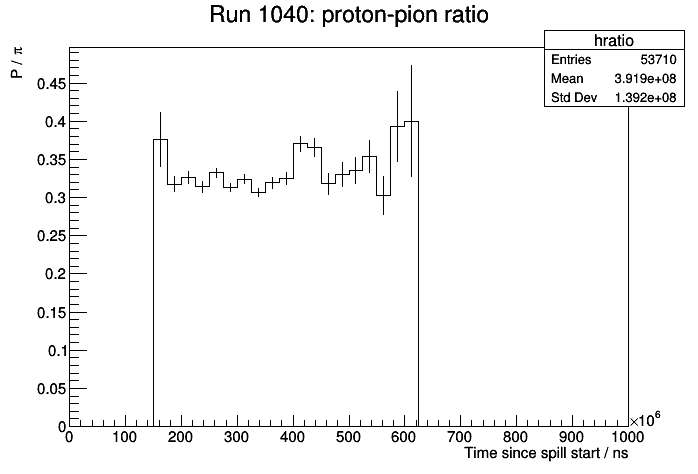
\includegraphics[width=\textwidth]{files/Figures/Run1040_proPiRatio}
	%		\caption{The ratio of protons to pions as a function of time since the start of the beam spill. For these data, 1 moderator block was in place and the beam momentum was nominally 0.8~GeV/c. The data for this graph is from the sum of 255 spills.}
	%		\label{fig:proPiRatio}
	%	\end{minipage} 
	%	\hspace{0.3cm}
	%	\begin{minipage}[t]{0.48\textwidth}
	%		\centering
	%		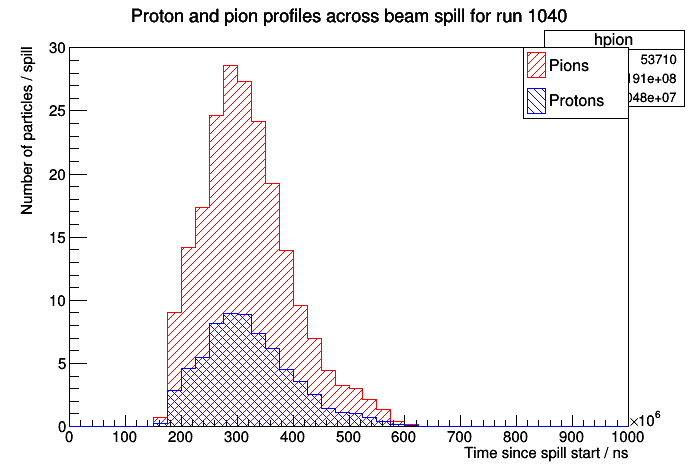
\includegraphics[width=\textwidth]{files/Figures/Run1040_proPiProf}
	%		\caption{The number of protons and pions detected per spill by the DsToF as a function of time since the start of the beam spill. For these data, 1 moderator block was in place and the beam momentum was nominally 0.8~GeV/c. The data for this graph is from the sum of 255 spills.}
	%		\label{fig:proPiProf}
	%	\end{minipage}
	%\end{figure}
   
	Figure~\ref{fig:thetas4mip} shows the flux of particles identified as minimum ionizing particles across $S4$.
	This flux is shown as as a function of the angle in the $x-y$ plane (see figure~\ref{fig:setup} for the definitions of these axes) for varying numbers of moderator blocks.
	For all numbers of moderator blocks, the peak number of minimum ionizing particle events occurs at a value of $\theta$ between $1^{\circ}$ and $2^{\circ}$.
	Similarly the number of proton events per spill, shown in figure~\ref{fig:thetas4pro} peaks at a value of $\theta$ of approximately $2^{\circ}$.
	
	Two factors have an impact on the position of the peak:
	the limited efficiency of $S4$ at the ends of the bars (near to either of the photomultiplier tubes) causes a smaller fraction of signal hits to be recorded in these regions. 
	This limited efficiency is caused by the requirement that both PMTs record a waveform in order for a signal to be recorded.
	This requirement is made, in order to reduce the number of false positives from dark noise in the bar.
	
	The angular overlap of $S2$ and $S4$ also plays a role in the position of the peak. 
	Figure~\ref{fig:beamAng} shows that, when observed from $S1$, a limited area of $S4$ is shadowed by the active area of $S2$.
	Given the requirement that a signal must be observed in $S2$, it is clear that the majority of events that are observed in $S4$ are from this overlap region.
   
   	Figure~\ref{fig:thetas4mip} also indicates that an increasing number of moderator blocks results in an increased total MIP flux through $S4$.
   	This is observed due to the off-axis position of both $S2$ and $S4$ avoids much of the unmoderated beam particles striking these timing points.
   	Due to scattering processes in the moderator, a greater number of MIPs are incident upon $S2$ and $S4$, with more scattering occurring with greater numbers of moderator blocks
   	
   	When changing from an unmoderated beam to the configuration with 1 moderator block, the proton flux shown in figure~\ref{fig:thetas4pro} initially sees an increase in the total number of events in $S4$.
   	However, upon the addition of further moderator blocks, the total number of proton events observed in $S4$ falls.
   	The initial increase is thought to be for similar reasons to those specified for the MIP flux, with increased scattering causing more protons to pass through the off-axis $S2$ and $S4$.
   	The subsequent decrease is likely due to the larger loss of energy of the protons in the thicker moderator.
   	In turn, this may lead to attenuation of protons in the TPC resulting in fewer observed events in $S4$.
   
   	\begin{figure}[ht]
   		\begin{minipage}[t]{0.48\textwidth}
   			\begin{adjustbox}{max totalsize={\textwidth}{.35\textheight},center}
		   		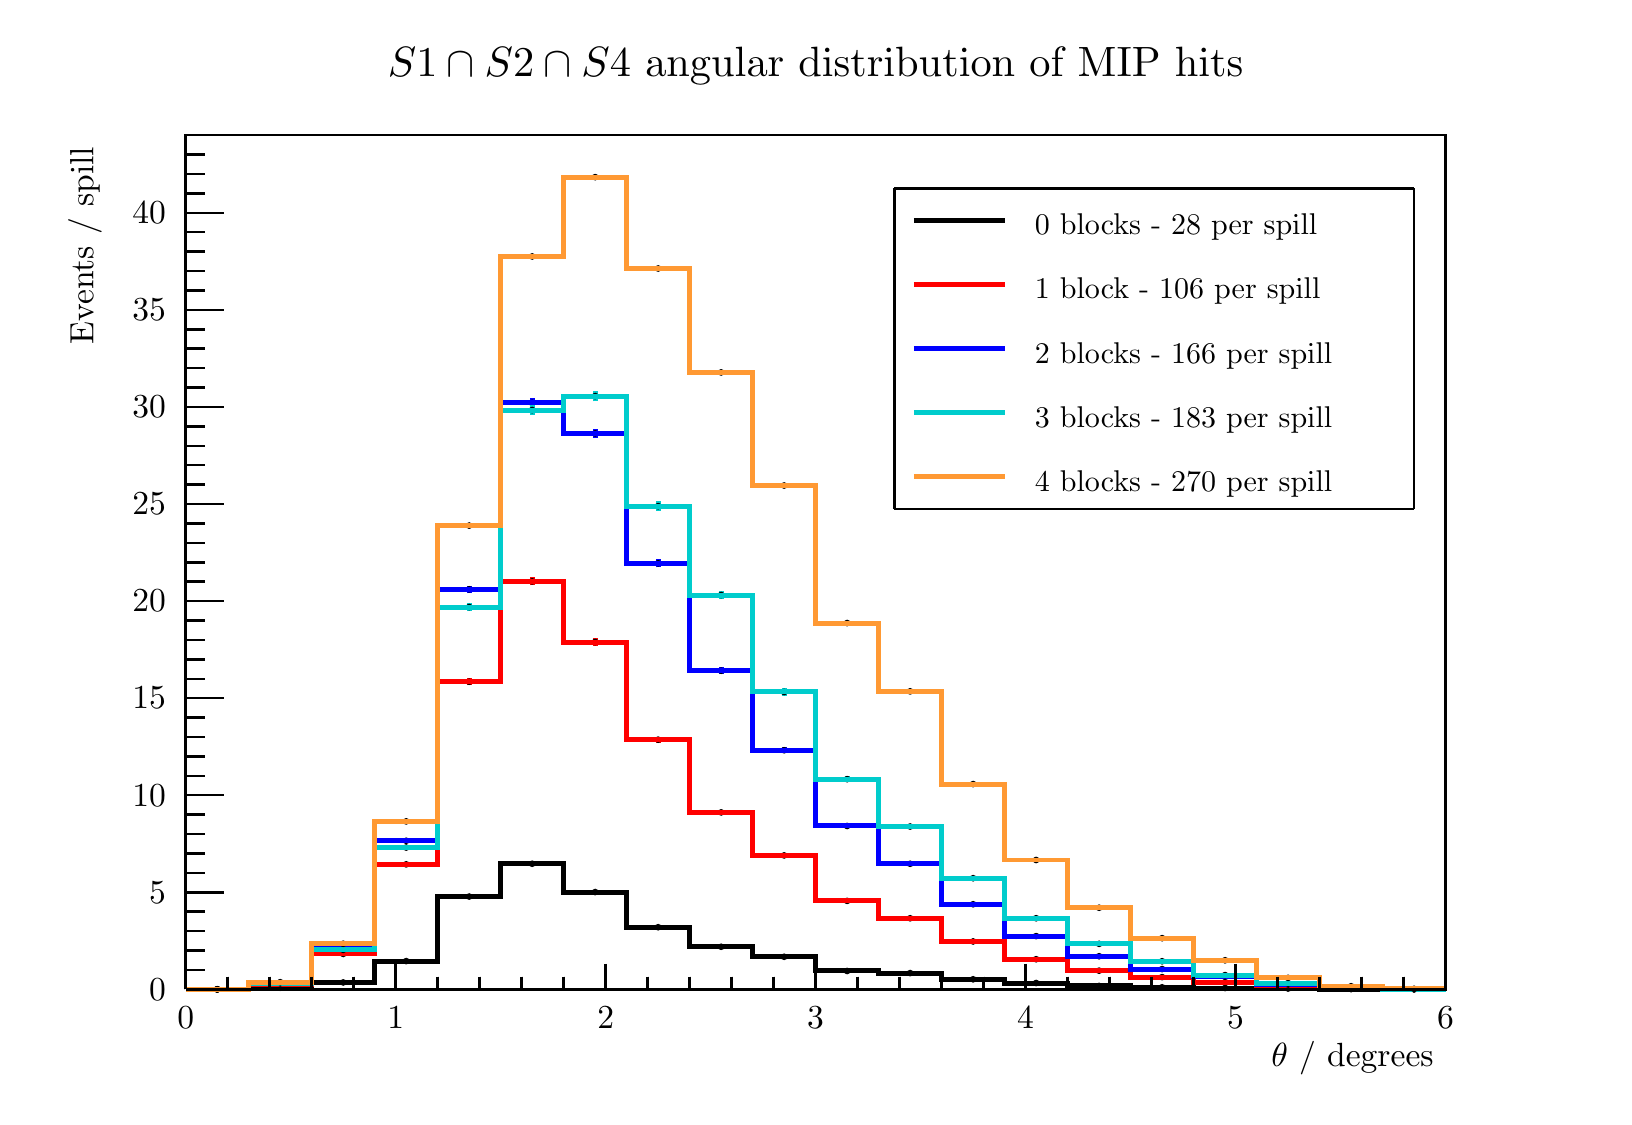
\begin{tikzpicture}
\pgfdeclareplotmark{cross} {
\pgfpathmoveto{\pgfpoint{-0.3\pgfplotmarksize}{\pgfplotmarksize}}
\pgfpathlineto{\pgfpoint{+0.3\pgfplotmarksize}{\pgfplotmarksize}}
\pgfpathlineto{\pgfpoint{+0.3\pgfplotmarksize}{0.3\pgfplotmarksize}}
\pgfpathlineto{\pgfpoint{+1\pgfplotmarksize}{0.3\pgfplotmarksize}}
\pgfpathlineto{\pgfpoint{+1\pgfplotmarksize}{-0.3\pgfplotmarksize}}
\pgfpathlineto{\pgfpoint{+0.3\pgfplotmarksize}{-0.3\pgfplotmarksize}}
\pgfpathlineto{\pgfpoint{+0.3\pgfplotmarksize}{-1.\pgfplotmarksize}}
\pgfpathlineto{\pgfpoint{-0.3\pgfplotmarksize}{-1.\pgfplotmarksize}}
\pgfpathlineto{\pgfpoint{-0.3\pgfplotmarksize}{-0.3\pgfplotmarksize}}
\pgfpathlineto{\pgfpoint{-1.\pgfplotmarksize}{-0.3\pgfplotmarksize}}
\pgfpathlineto{\pgfpoint{-1.\pgfplotmarksize}{0.3\pgfplotmarksize}}
\pgfpathlineto{\pgfpoint{-0.3\pgfplotmarksize}{0.3\pgfplotmarksize}}
\pgfpathclose
\pgfusepathqstroke
}
\pgfdeclareplotmark{cross*} {
\pgfpathmoveto{\pgfpoint{-0.3\pgfplotmarksize}{\pgfplotmarksize}}
\pgfpathlineto{\pgfpoint{+0.3\pgfplotmarksize}{\pgfplotmarksize}}
\pgfpathlineto{\pgfpoint{+0.3\pgfplotmarksize}{0.3\pgfplotmarksize}}
\pgfpathlineto{\pgfpoint{+1\pgfplotmarksize}{0.3\pgfplotmarksize}}
\pgfpathlineto{\pgfpoint{+1\pgfplotmarksize}{-0.3\pgfplotmarksize}}
\pgfpathlineto{\pgfpoint{+0.3\pgfplotmarksize}{-0.3\pgfplotmarksize}}
\pgfpathlineto{\pgfpoint{+0.3\pgfplotmarksize}{-1.\pgfplotmarksize}}
\pgfpathlineto{\pgfpoint{-0.3\pgfplotmarksize}{-1.\pgfplotmarksize}}
\pgfpathlineto{\pgfpoint{-0.3\pgfplotmarksize}{-0.3\pgfplotmarksize}}
\pgfpathlineto{\pgfpoint{-1.\pgfplotmarksize}{-0.3\pgfplotmarksize}}
\pgfpathlineto{\pgfpoint{-1.\pgfplotmarksize}{0.3\pgfplotmarksize}}
\pgfpathlineto{\pgfpoint{-0.3\pgfplotmarksize}{0.3\pgfplotmarksize}}
\pgfpathclose
\pgfusepathqfillstroke
}
\pgfdeclareplotmark{newstar} {
\pgfpathmoveto{\pgfqpoint{0pt}{\pgfplotmarksize}}
\pgfpathlineto{\pgfqpointpolar{44}{0.5\pgfplotmarksize}}
\pgfpathlineto{\pgfqpointpolar{18}{\pgfplotmarksize}}
\pgfpathlineto{\pgfqpointpolar{-20}{0.5\pgfplotmarksize}}
\pgfpathlineto{\pgfqpointpolar{-54}{\pgfplotmarksize}}
\pgfpathlineto{\pgfqpointpolar{-90}{0.5\pgfplotmarksize}}
\pgfpathlineto{\pgfqpointpolar{234}{\pgfplotmarksize}}
\pgfpathlineto{\pgfqpointpolar{198}{0.5\pgfplotmarksize}}
\pgfpathlineto{\pgfqpointpolar{162}{\pgfplotmarksize}}
\pgfpathlineto{\pgfqpointpolar{134}{0.5\pgfplotmarksize}}
\pgfpathclose
\pgfusepathqstroke
}
\pgfdeclareplotmark{newstar*} {
\pgfpathmoveto{\pgfqpoint{0pt}{\pgfplotmarksize}}
\pgfpathlineto{\pgfqpointpolar{44}{0.5\pgfplotmarksize}}
\pgfpathlineto{\pgfqpointpolar{18}{\pgfplotmarksize}}
\pgfpathlineto{\pgfqpointpolar{-20}{0.5\pgfplotmarksize}}
\pgfpathlineto{\pgfqpointpolar{-54}{\pgfplotmarksize}}
\pgfpathlineto{\pgfqpointpolar{-90}{0.5\pgfplotmarksize}}
\pgfpathlineto{\pgfqpointpolar{234}{\pgfplotmarksize}}
\pgfpathlineto{\pgfqpointpolar{198}{0.5\pgfplotmarksize}}
\pgfpathlineto{\pgfqpointpolar{162}{\pgfplotmarksize}}
\pgfpathlineto{\pgfqpointpolar{134}{0.5\pgfplotmarksize}}
\pgfpathclose
\pgfusepathqfillstroke
}
\definecolor{c}{rgb}{1,1,1};
\draw [color=c, fill=c] (0,0) rectangle (20,13.5632);
\draw [color=c, fill=c] (2,1.35632) rectangle (18,12.2069);
\definecolor{c}{rgb}{0,0,0};
\draw [c,line width=0.9] (2,1.35632) -- (2,12.2069) -- (18,12.2069) -- (18,1.35632) -- (2,1.35632);
\definecolor{c}{rgb}{1,1,1};
\draw [color=c, fill=c] (2,1.35632) rectangle (18,12.2069);
\definecolor{c}{rgb}{0,0,0};
\draw [c,line width=0.9] (2,1.35632) -- (2,12.2069) -- (18,12.2069) -- (18,1.35632) -- (2,1.35632);
\definecolor{c}{rgb}{0,0,0.6};
\draw [c,line width=0.9] (2,1.35632) -- (2.8,1.35632) -- (2.8,1.35632) -- (3.6,1.35632) -- (3.6,1.35632) -- (4.4,1.35632) -- (4.4,1.35632) -- (5.2,1.35632) -- (5.2,1.35632) -- (6,1.35632) -- (6,1.35632) -- (6.8,1.35632) -- (6.8,1.35632) --
 (7.6,1.35632) -- (7.6,1.35632) -- (8.4,1.35632) -- (8.4,1.35632) -- (9.2,1.35632) -- (9.2,1.35632) -- (10,1.35632) -- (10,1.35632) -- (10.8,1.35632) -- (10.8,1.35632) -- (11.6,1.35632) -- (11.6,1.35632) -- (12.4,1.35632) -- (12.4,1.35632) --
 (13.2,1.35632) -- (13.2,1.35632) -- (14,1.35632) -- (14,1.35632) -- (14.8,1.35632) -- (14.8,1.35632) -- (15.6,1.35632) -- (15.6,1.35632) -- (16.4,1.35632) -- (16.4,1.35632) -- (17.2,1.35632) -- (17.2,1.35632) -- (18,1.35632);
\definecolor{c}{rgb}{0,0,0};
\draw [c,line width=0.9] (2,1.35632) -- (18,1.35632);
\draw [anchor= east] (18,0.488276) node[scale=1.2126, color=c, rotate=0]{$\theta$ / degrees};
\draw [c,line width=0.9] (2,1.68184) -- (2,1.35632);
\draw [c,line width=0.9] (2.53333,1.51908) -- (2.53333,1.35632);
\draw [c,line width=0.9] (3.06667,1.51908) -- (3.06667,1.35632);
\draw [c,line width=0.9] (3.6,1.51908) -- (3.6,1.35632);
\draw [c,line width=0.9] (4.13333,1.51908) -- (4.13333,1.35632);
\draw [c,line width=0.9] (4.66667,1.68184) -- (4.66667,1.35632);
\draw [c,line width=0.9] (5.2,1.51908) -- (5.2,1.35632);
\draw [c,line width=0.9] (5.73333,1.51908) -- (5.73333,1.35632);
\draw [c,line width=0.9] (6.26667,1.51908) -- (6.26667,1.35632);
\draw [c,line width=0.9] (6.8,1.51908) -- (6.8,1.35632);
\draw [c,line width=0.9] (7.33333,1.68184) -- (7.33333,1.35632);
\draw [c,line width=0.9] (7.86667,1.51908) -- (7.86667,1.35632);
\draw [c,line width=0.9] (8.4,1.51908) -- (8.4,1.35632);
\draw [c,line width=0.9] (8.93333,1.51908) -- (8.93333,1.35632);
\draw [c,line width=0.9] (9.46667,1.51908) -- (9.46667,1.35632);
\draw [c,line width=0.9] (10,1.68184) -- (10,1.35632);
\draw [c,line width=0.9] (10.5333,1.51908) -- (10.5333,1.35632);
\draw [c,line width=0.9] (11.0667,1.51908) -- (11.0667,1.35632);
\draw [c,line width=0.9] (11.6,1.51908) -- (11.6,1.35632);
\draw [c,line width=0.9] (12.1333,1.51908) -- (12.1333,1.35632);
\draw [c,line width=0.9] (12.6667,1.68184) -- (12.6667,1.35632);
\draw [c,line width=0.9] (13.2,1.51908) -- (13.2,1.35632);
\draw [c,line width=0.9] (13.7333,1.51908) -- (13.7333,1.35632);
\draw [c,line width=0.9] (14.2667,1.51908) -- (14.2667,1.35632);
\draw [c,line width=0.9] (14.8,1.51908) -- (14.8,1.35632);
\draw [c,line width=0.9] (15.3333,1.68184) -- (15.3333,1.35632);
\draw [c,line width=0.9] (15.8667,1.51908) -- (15.8667,1.35632);
\draw [c,line width=0.9] (16.4,1.51908) -- (16.4,1.35632);
\draw [c,line width=0.9] (16.9333,1.51908) -- (16.9333,1.35632);
\draw [c,line width=0.9] (17.4667,1.51908) -- (17.4667,1.35632);
\draw [c,line width=0.9] (18,1.68184) -- (18,1.35632);
\draw [anchor=base] (2,0.854483) node[scale=1.2126, color=c, rotate=0]{0};
\draw [anchor=base] (4.66667,0.854483) node[scale=1.2126, color=c, rotate=0]{1};
\draw [anchor=base] (7.33333,0.854483) node[scale=1.2126, color=c, rotate=0]{2};
\draw [anchor=base] (10,0.854483) node[scale=1.2126, color=c, rotate=0]{3};
\draw [anchor=base] (12.6667,0.854483) node[scale=1.2126, color=c, rotate=0]{4};
\draw [anchor=base] (15.3333,0.854483) node[scale=1.2126, color=c, rotate=0]{5};
\draw [anchor=base] (18,0.854483) node[scale=1.2126, color=c, rotate=0]{6};
\draw [c,line width=0.9] (2,1.35632) -- (2,12.2069);
\draw [anchor= east] (0.72,12.2069) node[scale=1.2126, color=c, rotate=90]{ Events / spill};
\draw [c,line width=0.9] (2.48,1.35632) -- (2,1.35632);
\draw [c,line width=0.9] (2.24,1.60289) -- (2,1.60289);
\draw [c,line width=0.9] (2.24,1.84945) -- (2,1.84945);
\draw [c,line width=0.9] (2.24,2.09602) -- (2,2.09602);
\draw [c,line width=0.9] (2.24,2.34258) -- (2,2.34258);
\draw [c,line width=0.9] (2.48,2.58915) -- (2,2.58915);
\draw [c,line width=0.9] (2.24,2.83571) -- (2,2.83571);
\draw [c,line width=0.9] (2.24,3.08228) -- (2,3.08228);
\draw [c,line width=0.9] (2.24,3.32884) -- (2,3.32884);
\draw [c,line width=0.9] (2.24,3.57541) -- (2,3.57541);
\draw [c,line width=0.9] (2.48,3.82197) -- (2,3.82197);
\draw [c,line width=0.9] (2.24,4.06854) -- (2,4.06854);
\draw [c,line width=0.9] (2.24,4.31511) -- (2,4.31511);
\draw [c,line width=0.9] (2.24,4.56167) -- (2,4.56167);
\draw [c,line width=0.9] (2.24,4.80824) -- (2,4.80824);
\draw [c,line width=0.9] (2.48,5.0548) -- (2,5.0548);
\draw [c,line width=0.9] (2.24,5.30137) -- (2,5.30137);
\draw [c,line width=0.9] (2.24,5.54793) -- (2,5.54793);
\draw [c,line width=0.9] (2.24,5.7945) -- (2,5.7945);
\draw [c,line width=0.9] (2.24,6.04106) -- (2,6.04106);
\draw [c,line width=0.9] (2.48,6.28763) -- (2,6.28763);
\draw [c,line width=0.9] (2.24,6.53419) -- (2,6.53419);
\draw [c,line width=0.9] (2.24,6.78076) -- (2,6.78076);
\draw [c,line width=0.9] (2.24,7.02732) -- (2,7.02732);
\draw [c,line width=0.9] (2.24,7.27389) -- (2,7.27389);
\draw [c,line width=0.9] (2.48,7.52045) -- (2,7.52045);
\draw [c,line width=0.9] (2.24,7.76702) -- (2,7.76702);
\draw [c,line width=0.9] (2.24,8.01359) -- (2,8.01359);
\draw [c,line width=0.9] (2.24,8.26015) -- (2,8.26015);
\draw [c,line width=0.9] (2.24,8.50672) -- (2,8.50672);
\draw [c,line width=0.9] (2.48,8.75328) -- (2,8.75328);
\draw [c,line width=0.9] (2.24,8.99985) -- (2,8.99985);
\draw [c,line width=0.9] (2.24,9.24641) -- (2,9.24641);
\draw [c,line width=0.9] (2.24,9.49298) -- (2,9.49298);
\draw [c,line width=0.9] (2.24,9.73954) -- (2,9.73954);
\draw [c,line width=0.9] (2.48,9.98611) -- (2,9.98611);
\draw [c,line width=0.9] (2.24,10.2327) -- (2,10.2327);
\draw [c,line width=0.9] (2.24,10.4792) -- (2,10.4792);
\draw [c,line width=0.9] (2.24,10.7258) -- (2,10.7258);
\draw [c,line width=0.9] (2.24,10.9724) -- (2,10.9724);
\draw [c,line width=0.9] (2.48,11.2189) -- (2,11.2189);
\draw [c,line width=0.9] (2.48,11.2189) -- (2,11.2189);
\draw [c,line width=0.9] (2.24,11.4655) -- (2,11.4655);
\draw [c,line width=0.9] (2.24,11.7121) -- (2,11.7121);
\draw [c,line width=0.9] (2.24,11.9586) -- (2,11.9586);
\draw [c,line width=0.9] (2.24,12.2052) -- (2,12.2052);
\draw [anchor= east] (1.9,1.35632) node[scale=1.2126, color=c, rotate=0]{0};
\draw [anchor= east] (1.9,2.58915) node[scale=1.2126, color=c, rotate=0]{5};
\draw [anchor= east] (1.9,3.82197) node[scale=1.2126, color=c, rotate=0]{10};
\draw [anchor= east] (1.9,5.0548) node[scale=1.2126, color=c, rotate=0]{15};
\draw [anchor= east] (1.9,6.28763) node[scale=1.2126, color=c, rotate=0]{20};
\draw [anchor= east] (1.9,7.52045) node[scale=1.2126, color=c, rotate=0]{25};
\draw [anchor= east] (1.9,8.75328) node[scale=1.2126, color=c, rotate=0]{30};
\draw [anchor= east] (1.9,9.98611) node[scale=1.2126, color=c, rotate=0]{35};
\draw [anchor= east] (1.9,11.2189) node[scale=1.2126, color=c, rotate=0]{40};
\draw [c,line width=1.8] (2.4,1.35632) -- (2.4,1.35667);
\draw [c,line width=1.8] (2.4,1.35667) -- (2.4,1.35701);
\foreach \P in {(2.4,1.35667)}{\draw[mark options={color=c,fill=c},mark size=2.402402pt,mark=*,mark size=1pt] plot coordinates {\P};}
\draw [c,line width=1.8] (3.2,1.37421) -- (3.2,1.37732);
\draw [c,line width=1.8] (3.2,1.37732) -- (3.2,1.38043);
\foreach \P in {(3.2,1.37732)}{\draw[mark options={color=c,fill=c},mark size=2.402402pt,mark=*,mark size=1pt] plot coordinates {\P};}
\draw [c,line width=1.8] (4,1.43826) -- (4,1.44474);
\draw [c,line width=1.8] (4,1.44474) -- (4,1.45123);
\foreach \P in {(4,1.44474)}{\draw[mark options={color=c,fill=c},mark size=2.402402pt,mark=*,mark size=1pt] plot coordinates {\P};}
\draw [c,line width=1.8] (4.8,1.70111) -- (4.8,1.71559);
\draw [c,line width=1.8] (4.8,1.71559) -- (4.8,1.73006);
\foreach \P in {(4.8,1.71559)}{\draw[mark options={color=c,fill=c},mark size=2.402402pt,mark=*,mark size=1pt] plot coordinates {\P};}
\draw [c,line width=1.8] (5.6,2.50801) -- (5.6,2.53547);
\draw [c,line width=1.8] (5.6,2.53547) -- (5.6,2.56293);
\foreach \P in {(5.6,2.53547)}{\draw[mark options={color=c,fill=c},mark size=2.402402pt,mark=*,mark size=1pt] plot coordinates {\P};}
\draw [c,line width=1.8] (6.4,2.91977) -- (6.4,2.95217);
\draw [c,line width=1.8] (6.4,2.95217) -- (6.4,2.98457);
\foreach \P in {(6.4,2.95217)}{\draw[mark options={color=c,fill=c},mark size=2.402402pt,mark=*,mark size=1pt] plot coordinates {\P};}
\draw [c,line width=1.8] (7.2,2.56376) -- (7.2,2.59229);
\draw [c,line width=1.8] (7.2,2.59229) -- (7.2,2.62081);
\foreach \P in {(7.2,2.59229)}{\draw[mark options={color=c,fill=c},mark size=2.402402pt,mark=*,mark size=1pt] plot coordinates {\P};}
\draw [c,line width=1.8] (8,2.12349) -- (8,2.14597);
\draw [c,line width=1.8] (8,2.14597) -- (8,2.16846);
\foreach \P in {(8,2.14597)}{\draw[mark options={color=c,fill=c},mark size=2.402402pt,mark=*,mark size=1pt] plot coordinates {\P};}
\draw [c,line width=1.8] (8.8,1.87945) -- (8.8,1.89768);
\draw [c,line width=1.8] (8.8,1.89768) -- (8.8,1.91591);
\foreach \P in {(8.8,1.89768)}{\draw[mark options={color=c,fill=c},mark size=2.402402pt,mark=*,mark size=1pt] plot coordinates {\P};}
\draw [c,line width=1.8] (9.6,1.75482) -- (9.6,1.77052);
\draw [c,line width=1.8] (9.6,1.77052) -- (9.6,1.78623);
\foreach \P in {(9.6,1.77052)}{\draw[mark options={color=c,fill=c},mark size=2.402402pt,mark=*,mark size=1pt] plot coordinates {\P};}
\draw [c,line width=1.8] (10.4,1.57888) -- (10.4,1.59008);
\draw [c,line width=1.8] (10.4,1.59008) -- (10.4,1.60128);
\foreach \P in {(10.4,1.59008)}{\draw[mark options={color=c,fill=c},mark size=2.402402pt,mark=*,mark size=1pt] plot coordinates {\P};}
\draw [c,line width=1.8] (11.2,1.55242) -- (11.2,1.56325);
\draw [c,line width=1.8] (11.2,1.56325) -- (11.2,1.57407);
\foreach \P in {(11.2,1.56325)}{\draw[mark options={color=c,fill=c},mark size=2.402402pt,mark=*,mark size=1pt] plot coordinates {\P};}
\draw [c,line width=1.8] (12,1.4762) -- (12,1.48457);
\draw [c,line width=1.8] (12,1.48457) -- (12,1.49294);
\foreach \P in {(12,1.48457)}{\draw[mark options={color=c,fill=c},mark size=2.402402pt,mark=*,mark size=1pt] plot coordinates {\P};}
\draw [c,line width=1.8] (12.8,1.43085) -- (12.8,1.43719);
\draw [c,line width=1.8] (12.8,1.43719) -- (12.8,1.44352);
\foreach \P in {(12.8,1.43719)}{\draw[mark options={color=c,fill=c},mark size=2.402402pt,mark=*,mark size=1pt] plot coordinates {\P};}
\draw [c,line width=1.8] (13.6,1.396) -- (13.6,1.40053);
\draw [c,line width=1.8] (13.6,1.40053) -- (13.6,1.40507);
\foreach \P in {(13.6,1.40053)}{\draw[mark options={color=c,fill=c},mark size=2.402402pt,mark=*,mark size=1pt] plot coordinates {\P};}
\draw [c,line width=1.8] (14.4,1.3793) -- (14.4,1.38292);
\draw [c,line width=1.8] (14.4,1.38292) -- (14.4,1.38654);
\foreach \P in {(14.4,1.38292)}{\draw[mark options={color=c,fill=c},mark size=2.402402pt,mark=*,mark size=1pt] plot coordinates {\P};}
\draw [c,line width=1.8] (15.2,1.37113) -- (15.2,1.37379);
\draw [c,line width=1.8] (15.2,1.37379) -- (15.2,1.37645);
\foreach \P in {(15.2,1.37379)}{\draw[mark options={color=c,fill=c},mark size=2.402402pt,mark=*,mark size=1pt] plot coordinates {\P};}
\draw [c,line width=1.8] (16,1.3653) -- (16,1.36731);
\draw [c,line width=1.8] (16,1.36731) -- (16,1.36933);
\foreach \P in {(16,1.36731)}{\draw[mark options={color=c,fill=c},mark size=2.402402pt,mark=*,mark size=1pt] plot coordinates {\P};}
\draw [c,line width=1.8] (16.8,1.35901) -- (16.8,1.36043);
\draw [c,line width=1.8] (16.8,1.36043) -- (16.8,1.36184);
\foreach \P in {(16.8,1.36043)}{\draw[mark options={color=c,fill=c},mark size=2.402402pt,mark=*,mark size=1pt] plot coordinates {\P};}
\draw [c,line width=1.8] (2,1.35632) -- (2.8,1.35632) -- (2.8,1.37732) -- (3.6,1.37732) -- (3.6,1.44474) -- (4.4,1.44474) -- (4.4,1.71559) -- (5.2,1.71559) -- (5.2,2.53547) -- (6,2.53547) -- (6,2.95217) -- (6.8,2.95217) -- (6.8,2.59229) --
 (7.6,2.59229) -- (7.6,2.14597) -- (8.4,2.14597) -- (8.4,1.89768) -- (9.2,1.89768) -- (9.2,1.77052) -- (10,1.77052) -- (10,1.59008) -- (10.8,1.59008) -- (10.8,1.56325) -- (11.6,1.56325) -- (11.6,1.48457) -- (12.4,1.48457) -- (12.4,1.43719) --
 (13.2,1.43719) -- (13.2,1.40053) -- (14,1.40053) -- (14,1.38292) -- (14.8,1.38292) -- (14.8,1.37379) -- (15.6,1.37379) -- (15.6,1.36731) -- (16.4,1.36731) -- (16.4,1.36043) -- (17.2,1.36043) -- (17.2,1.35632) -- (18,1.35632);
\definecolor{c}{rgb}{1,0,0};
\draw [c,line width=1.8] (2.4,1.35632) -- (2.4,1.35684);
\draw [c,line width=1.8] (2.4,1.35684) -- (2.4,1.35736);
\definecolor{c}{rgb}{0,0,0};
\foreach \P in {(2.4,1.35684)}{\draw[mark options={color=c,fill=c},mark size=2.402402pt,mark=*,mark size=1pt] plot coordinates {\P};}
\definecolor{c}{rgb}{1,0,0};
\draw [c,line width=1.8] (3.2,1.41399) -- (3.2,1.41942);
\draw [c,line width=1.8] (3.2,1.41942) -- (3.2,1.42485);
\definecolor{c}{rgb}{0,0,0};
\foreach \P in {(3.2,1.41942)}{\draw[mark options={color=c,fill=c},mark size=2.402402pt,mark=*,mark size=1pt] plot coordinates {\P};}
\definecolor{c}{rgb}{1,0,0};
\draw [c,line width=1.8] (4,1.79246) -- (4,1.8069);
\draw [c,line width=1.8] (4,1.8069) -- (4,1.82134);
\definecolor{c}{rgb}{0,0,0};
\foreach \P in {(4,1.8069)}{\draw[mark options={color=c,fill=c},mark size=2.402402pt,mark=*,mark size=1pt] plot coordinates {\P};}
\definecolor{c}{rgb}{1,0,0};
\draw [c,line width=1.8] (4.8,2.9168) -- (4.8,2.94435);
\draw [c,line width=1.8] (4.8,2.94435) -- (4.8,2.9719);
\definecolor{c}{rgb}{0,0,0};
\foreach \P in {(4.8,2.94435)}{\draw[mark options={color=c,fill=c},mark size=2.402402pt,mark=*,mark size=1pt] plot coordinates {\P};}
\definecolor{c}{rgb}{1,0,0};
\draw [c,line width=1.8] (5.6,5.21998) -- (5.6,5.26355);
\draw [c,line width=1.8] (5.6,5.26355) -- (5.6,5.30712);
\definecolor{c}{rgb}{0,0,0};
\foreach \P in {(5.6,5.26355)}{\draw[mark options={color=c,fill=c},mark size=2.402402pt,mark=*,mark size=1pt] plot coordinates {\P};}
\definecolor{c}{rgb}{1,0,0};
\draw [c,line width=1.8] (6.4,6.48763) -- (6.4,6.53825);
\draw [c,line width=1.8] (6.4,6.53825) -- (6.4,6.58887);
\definecolor{c}{rgb}{0,0,0};
\foreach \P in {(6.4,6.53825)}{\draw[mark options={color=c,fill=c},mark size=2.402402pt,mark=*,mark size=1pt] plot coordinates {\P};}
\definecolor{c}{rgb}{1,0,0};
\draw [c,line width=1.8] (7.2,5.7211) -- (7.2,5.76788);
\draw [c,line width=1.8] (7.2,5.76788) -- (7.2,5.81465);
\definecolor{c}{rgb}{0,0,0};
\foreach \P in {(7.2,5.76788)}{\draw[mark options={color=c,fill=c},mark size=2.402402pt,mark=*,mark size=1pt] plot coordinates {\P};}
\definecolor{c}{rgb}{1,0,0};
\draw [c,line width=1.8] (8,4.48824) -- (8,4.52785);
\draw [c,line width=1.8] (8,4.52785) -- (8,4.56745);
\definecolor{c}{rgb}{0,0,0};
\foreach \P in {(8,4.52785)}{\draw[mark options={color=c,fill=c},mark size=2.402402pt,mark=*,mark size=1pt] plot coordinates {\P};}
\definecolor{c}{rgb}{1,0,0};
\draw [c,line width=1.8] (8.8,3.57095) -- (8.8,3.60412);
\draw [c,line width=1.8] (8.8,3.60412) -- (8.8,3.63729);
\definecolor{c}{rgb}{0,0,0};
\foreach \P in {(8.8,3.60412)}{\draw[mark options={color=c,fill=c},mark size=2.402402pt,mark=*,mark size=1pt] plot coordinates {\P};}
\definecolor{c}{rgb}{1,0,0};
\draw [c,line width=1.8] (9.6,3.02904) -- (9.6,3.0578);
\draw [c,line width=1.8] (9.6,3.0578) -- (9.6,3.08655);
\definecolor{c}{rgb}{0,0,0};
\foreach \P in {(9.6,3.0578)}{\draw[mark options={color=c,fill=c},mark size=2.402402pt,mark=*,mark size=1pt] plot coordinates {\P};}
\definecolor{c}{rgb}{1,0,0};
\draw [c,line width=1.8] (10.4,2.45738) -- (10.4,2.48051);
\draw [c,line width=1.8] (10.4,2.48051) -- (10.4,2.50364);
\definecolor{c}{rgb}{0,0,0};
\foreach \P in {(10.4,2.48051)}{\draw[mark options={color=c,fill=c},mark size=2.402402pt,mark=*,mark size=1pt] plot coordinates {\P};}
\definecolor{c}{rgb}{1,0,0};
\draw [c,line width=1.8] (11.2,2.23876) -- (11.2,2.25958);
\draw [c,line width=1.8] (11.2,2.25958) -- (11.2,2.2804);
\definecolor{c}{rgb}{0,0,0};
\foreach \P in {(11.2,2.25958)}{\draw[mark options={color=c,fill=c},mark size=2.402402pt,mark=*,mark size=1pt] plot coordinates {\P};}
\definecolor{c}{rgb}{1,0,0};
\draw [c,line width=1.8] (12,1.9482) -- (12,1.96524);
\draw [c,line width=1.8] (12,1.96524) -- (12,1.98228);
\definecolor{c}{rgb}{0,0,0};
\foreach \P in {(12,1.96524)}{\draw[mark options={color=c,fill=c},mark size=2.402402pt,mark=*,mark size=1pt] plot coordinates {\P};}
\definecolor{c}{rgb}{1,0,0};
\draw [c,line width=1.8] (12.8,1.72599) -- (12.8,1.73946);
\draw [c,line width=1.8] (12.8,1.73946) -- (12.8,1.75293);
\definecolor{c}{rgb}{0,0,0};
\foreach \P in {(12.8,1.73946)}{\draw[mark options={color=c,fill=c},mark size=2.402402pt,mark=*,mark size=1pt] plot coordinates {\P};}
\definecolor{c}{rgb}{1,0,0};
\draw [c,line width=1.8] (13.6,1.58383) -- (13.6,1.59435);
\draw [c,line width=1.8] (13.6,1.59435) -- (13.6,1.60486);
\definecolor{c}{rgb}{0,0,0};
\foreach \P in {(13.6,1.59435)}{\draw[mark options={color=c,fill=c},mark size=2.402402pt,mark=*,mark size=1pt] plot coordinates {\P};}
\definecolor{c}{rgb}{1,0,0};
\draw [c,line width=1.8] (14.4,1.50365) -- (14.4,1.5122);
\draw [c,line width=1.8] (14.4,1.5122) -- (14.4,1.52075);
\definecolor{c}{rgb}{0,0,0};
\foreach \P in {(14.4,1.5122)}{\draw[mark options={color=c,fill=c},mark size=2.402402pt,mark=*,mark size=1pt] plot coordinates {\P};}
\definecolor{c}{rgb}{1,0,0};
\draw [c,line width=1.8] (15.2,1.44017) -- (15.2,1.44659);
\draw [c,line width=1.8] (15.2,1.44659) -- (15.2,1.45301);
\definecolor{c}{rgb}{0,0,0};
\foreach \P in {(15.2,1.44659)}{\draw[mark options={color=c,fill=c},mark size=2.402402pt,mark=*,mark size=1pt] plot coordinates {\P};}
\definecolor{c}{rgb}{1,0,0};
\draw [c,line width=1.8] (16,1.39317) -- (16,1.39741);
\draw [c,line width=1.8] (16,1.39741) -- (16,1.40165);
\definecolor{c}{rgb}{0,0,0};
\foreach \P in {(16,1.39741)}{\draw[mark options={color=c,fill=c},mark size=2.402402pt,mark=*,mark size=1pt] plot coordinates {\P};}
\definecolor{c}{rgb}{1,0,0};
\draw [c,line width=1.8] (16.8,1.36205) -- (16.8,1.36376);
\draw [c,line width=1.8] (16.8,1.36376) -- (16.8,1.36548);
\definecolor{c}{rgb}{0,0,0};
\foreach \P in {(16.8,1.36376)}{\draw[mark options={color=c,fill=c},mark size=2.402402pt,mark=*,mark size=1pt] plot coordinates {\P};}
\definecolor{c}{rgb}{1,0,0};
\draw [c,line width=1.8] (17.6,1.35734) -- (17.6,1.35821);
\draw [c,line width=1.8] (17.6,1.35821) -- (17.6,1.35909);
\definecolor{c}{rgb}{0,0,0};
\foreach \P in {(17.6,1.35821)}{\draw[mark options={color=c,fill=c},mark size=2.402402pt,mark=*,mark size=1pt] plot coordinates {\P};}
\definecolor{c}{rgb}{1,0,0};
\draw [c,line width=1.8] (2,1.35632) -- (2.8,1.35632) -- (2.8,1.41942) -- (3.6,1.41942) -- (3.6,1.8069) -- (4.4,1.8069) -- (4.4,2.94435) -- (5.2,2.94435) -- (5.2,5.26355) -- (6,5.26355) -- (6,6.53825) -- (6.8,6.53825) -- (6.8,5.76788) --
 (7.6,5.76788) -- (7.6,4.52785) -- (8.4,4.52785) -- (8.4,3.60412) -- (9.2,3.60412) -- (9.2,3.0578) -- (10,3.0578) -- (10,2.48051) -- (10.8,2.48051) -- (10.8,2.25958) -- (11.6,2.25958) -- (11.6,1.96524) -- (12.4,1.96524) -- (12.4,1.73946) --
 (13.2,1.73946) -- (13.2,1.59435) -- (14,1.59435) -- (14,1.5122) -- (14.8,1.5122) -- (14.8,1.44659) -- (15.6,1.44659) -- (15.6,1.39741) -- (16.4,1.39741) -- (16.4,1.36376) -- (17.2,1.36376) -- (17.2,1.35821) -- (18,1.35821);
\definecolor{c}{rgb}{0,0,1};
\draw [c,line width=1.8] (2.4,1.35708) -- (2.4,1.3579);
\draw [c,line width=1.8] (2.4,1.3579) -- (2.4,1.35872);
\definecolor{c}{rgb}{0,0,0};
\foreach \P in {(2.4,1.3579)}{\draw[mark options={color=c,fill=c},mark size=2.402402pt,mark=*,mark size=1pt] plot coordinates {\P};}
\definecolor{c}{rgb}{0,0,1};
\draw [c,line width=1.8] (3.2,1.4364) -- (3.2,1.44247);
\draw [c,line width=1.8] (3.2,1.44247) -- (3.2,1.44854);
\definecolor{c}{rgb}{0,0,0};
\foreach \P in {(3.2,1.44247)}{\draw[mark options={color=c,fill=c},mark size=2.402402pt,mark=*,mark size=1pt] plot coordinates {\P};}
\definecolor{c}{rgb}{0,0,1};
\draw [c,line width=1.8] (4,1.87947) -- (4,1.89447);
\draw [c,line width=1.8] (4,1.89447) -- (4,1.90948);
\definecolor{c}{rgb}{0,0,0};
\foreach \P in {(4,1.89447)}{\draw[mark options={color=c,fill=c},mark size=2.402402pt,mark=*,mark size=1pt] plot coordinates {\P};}
\definecolor{c}{rgb}{0,0,1};
\draw [c,line width=1.8] (4.8,3.21502) -- (4.8,3.24377);
\draw [c,line width=1.8] (4.8,3.24377) -- (4.8,3.27252);
\definecolor{c}{rgb}{0,0,0};
\foreach \P in {(4.8,3.24377)}{\draw[mark options={color=c,fill=c},mark size=2.402402pt,mark=*,mark size=1pt] plot coordinates {\P};}
\definecolor{c}{rgb}{0,0,1};
\draw [c,line width=1.8] (5.6,6.38923) -- (5.6,6.43726);
\draw [c,line width=1.8] (5.6,6.43726) -- (5.6,6.4853);
\definecolor{c}{rgb}{0,0,0};
\foreach \P in {(5.6,6.43726)}{\draw[mark options={color=c,fill=c},mark size=2.402402pt,mark=*,mark size=1pt] plot coordinates {\P};}
\definecolor{c}{rgb}{0,0,1};
\draw [c,line width=1.8] (6.4,8.74649) -- (6.4,8.80556);
\draw [c,line width=1.8] (6.4,8.80556) -- (6.4,8.86464);
\definecolor{c}{rgb}{0,0,0};
\foreach \P in {(6.4,8.80556)}{\draw[mark options={color=c,fill=c},mark size=2.402402pt,mark=*,mark size=1pt] plot coordinates {\P};}
\definecolor{c}{rgb}{0,0,1};
\draw [c,line width=1.8] (7.2,8.35944) -- (7.2,8.41733);
\draw [c,line width=1.8] (7.2,8.41733) -- (7.2,8.47523);
\definecolor{c}{rgb}{0,0,0};
\foreach \P in {(7.2,8.41733)}{\draw[mark options={color=c,fill=c},mark size=2.402402pt,mark=*,mark size=1pt] plot coordinates {\P};}
\definecolor{c}{rgb}{0,0,1};
\draw [c,line width=1.8] (8,6.71706) -- (8,6.76769);
\draw [c,line width=1.8] (8,6.76769) -- (8,6.81831);
\definecolor{c}{rgb}{0,0,0};
\foreach \P in {(8,6.76769)}{\draw[mark options={color=c,fill=c},mark size=2.402402pt,mark=*,mark size=1pt] plot coordinates {\P};}
\definecolor{c}{rgb}{0,0,1};
\draw [c,line width=1.8] (8.8,5.36035) -- (8.8,5.40382);
\draw [c,line width=1.8] (8.8,5.40382) -- (8.8,5.44729);
\definecolor{c}{rgb}{0,0,0};
\foreach \P in {(8.8,5.40382)}{\draw[mark options={color=c,fill=c},mark size=2.402402pt,mark=*,mark size=1pt] plot coordinates {\P};}
\definecolor{c}{rgb}{0,0,1};
\draw [c,line width=1.8] (9.6,4.35606) -- (9.6,4.39354);
\draw [c,line width=1.8] (9.6,4.39354) -- (9.6,4.43102);
\definecolor{c}{rgb}{0,0,0};
\foreach \P in {(9.6,4.39354)}{\draw[mark options={color=c,fill=c},mark size=2.402402pt,mark=*,mark size=1pt] plot coordinates {\P};}
\definecolor{c}{rgb}{0,0,1};
\draw [c,line width=1.8] (10.4,3.40078) -- (10.4,3.43159);
\draw [c,line width=1.8] (10.4,3.43159) -- (10.4,3.4624);
\definecolor{c}{rgb}{0,0,0};
\foreach \P in {(10.4,3.43159)}{\draw[mark options={color=c,fill=c},mark size=2.402402pt,mark=*,mark size=1pt] plot coordinates {\P};}
\definecolor{c}{rgb}{0,0,1};
\draw [c,line width=1.8] (11.2,2.92459) -- (11.2,2.95159);
\draw [c,line width=1.8] (11.2,2.95159) -- (11.2,2.9786);
\definecolor{c}{rgb}{0,0,0};
\foreach \P in {(11.2,2.95159)}{\draw[mark options={color=c,fill=c},mark size=2.402402pt,mark=*,mark size=1pt] plot coordinates {\P};}
\definecolor{c}{rgb}{0,0,1};
\draw [c,line width=1.8] (12,2.4153) -- (12,2.43751);
\draw [c,line width=1.8] (12,2.43751) -- (12,2.45973);
\definecolor{c}{rgb}{0,0,0};
\foreach \P in {(12,2.43751)}{\draw[mark options={color=c,fill=c},mark size=2.402402pt,mark=*,mark size=1pt] plot coordinates {\P};}
\definecolor{c}{rgb}{0,0,1};
\draw [c,line width=1.8] (12.8,2.01547) -- (12.8,2.03294);
\draw [c,line width=1.8] (12.8,2.03294) -- (12.8,2.05042);
\definecolor{c}{rgb}{0,0,0};
\foreach \P in {(12.8,2.03294)}{\draw[mark options={color=c,fill=c},mark size=2.402402pt,mark=*,mark size=1pt] plot coordinates {\P};}
\definecolor{c}{rgb}{0,0,1};
\draw [c,line width=1.8] (13.6,1.76361) -- (13.6,1.77737);
\draw [c,line width=1.8] (13.6,1.77737) -- (13.6,1.79112);
\definecolor{c}{rgb}{0,0,0};
\foreach \P in {(13.6,1.77737)}{\draw[mark options={color=c,fill=c},mark size=2.402402pt,mark=*,mark size=1pt] plot coordinates {\P};}
\definecolor{c}{rgb}{0,0,1};
\draw [c,line width=1.8] (14.4,1.6037) -- (14.4,1.61434);
\draw [c,line width=1.8] (14.4,1.61434) -- (14.4,1.62498);
\definecolor{c}{rgb}{0,0,0};
\foreach \P in {(14.4,1.61434)}{\draw[mark options={color=c,fill=c},mark size=2.402402pt,mark=*,mark size=1pt] plot coordinates {\P};}
\definecolor{c}{rgb}{0,0,1};
\draw [c,line width=1.8] (15.2,1.50924) -- (15.2,1.51757);
\draw [c,line width=1.8] (15.2,1.51757) -- (15.2,1.5259);
\definecolor{c}{rgb}{0,0,0};
\foreach \P in {(15.2,1.51757)}{\draw[mark options={color=c,fill=c},mark size=2.402402pt,mark=*,mark size=1pt] plot coordinates {\P};}
\definecolor{c}{rgb}{0,0,1};
\draw [c,line width=1.8] (16,1.41395) -- (16,1.41894);
\draw [c,line width=1.8] (16,1.41894) -- (16,1.42392);
\definecolor{c}{rgb}{0,0,0};
\foreach \P in {(16,1.41894)}{\draw[mark options={color=c,fill=c},mark size=2.402402pt,mark=*,mark size=1pt] plot coordinates {\P};}
\definecolor{c}{rgb}{0,0,1};
\draw [c,line width=1.8] (16.8,1.37118) -- (16.8,1.37369);
\draw [c,line width=1.8] (16.8,1.37369) -- (16.8,1.3762);
\definecolor{c}{rgb}{0,0,0};
\foreach \P in {(16.8,1.37369)}{\draw[mark options={color=c,fill=c},mark size=2.402402pt,mark=*,mark size=1pt] plot coordinates {\P};}
\definecolor{c}{rgb}{0,0,1};
\draw [c,line width=1.8] (17.6,1.35734) -- (17.6,1.35787);
\draw [c,line width=1.8] (17.6,1.35787) -- (17.6,1.3584);
\definecolor{c}{rgb}{0,0,0};
\foreach \P in {(17.6,1.35787)}{\draw[mark options={color=c,fill=c},mark size=2.402402pt,mark=*,mark size=1pt] plot coordinates {\P};}
\definecolor{c}{rgb}{0,0,1};
\draw [c,line width=1.8] (2,1.3579) -- (2.8,1.3579) -- (2.8,1.44247) -- (3.6,1.44247) -- (3.6,1.89447) -- (4.4,1.89447) -- (4.4,3.24377) -- (5.2,3.24377) -- (5.2,6.43726) -- (6,6.43726) -- (6,8.80556) -- (6.8,8.80556) -- (6.8,8.41733) --
 (7.6,8.41733) -- (7.6,6.76769) -- (8.4,6.76769) -- (8.4,5.40382) -- (9.2,5.40382) -- (9.2,4.39354) -- (10,4.39354) -- (10,3.43159) -- (10.8,3.43159) -- (10.8,2.95159) -- (11.6,2.95159) -- (11.6,2.43751) -- (12.4,2.43751) -- (12.4,2.03294) --
 (13.2,2.03294) -- (13.2,1.77737) -- (14,1.77737) -- (14,1.61434) -- (14.8,1.61434) -- (14.8,1.51757) -- (15.6,1.51757) -- (15.6,1.41894) -- (16.4,1.41894) -- (16.4,1.37369) -- (17.2,1.37369) -- (17.2,1.35787) -- (18,1.35787);
\definecolor{c}{rgb}{0,0.8,0.8};
\draw [c,line width=1.8] (2.4,1.35646) -- (2.4,1.3568);
\draw [c,line width=1.8] (2.4,1.3568) -- (2.4,1.35714);
\definecolor{c}{rgb}{0,0,0};
\foreach \P in {(2.4,1.3568)}{\draw[mark options={color=c,fill=c},mark size=2.402402pt,mark=*,mark size=1pt] plot coordinates {\P};}
\definecolor{c}{rgb}{0,0.8,0.8};
\draw [c,line width=1.8] (3.2,1.42647) -- (3.2,1.43272);
\draw [c,line width=1.8] (3.2,1.43272) -- (3.2,1.43898);
\definecolor{c}{rgb}{0,0,0};
\foreach \P in {(3.2,1.43272)}{\draw[mark options={color=c,fill=c},mark size=2.402402pt,mark=*,mark size=1pt] plot coordinates {\P};}
\definecolor{c}{rgb}{0,0.8,0.8};
\draw [c,line width=1.8] (4,1.84302) -- (4,1.85912);
\draw [c,line width=1.8] (4,1.85912) -- (4,1.87522);
\definecolor{c}{rgb}{0,0,0};
\foreach \P in {(4,1.85912)}{\draw[mark options={color=c,fill=c},mark size=2.402402pt,mark=*,mark size=1pt] plot coordinates {\P};}
\definecolor{c}{rgb}{0,0.8,0.8};
\draw [c,line width=1.8] (4.8,3.1265) -- (4.8,3.15769);
\draw [c,line width=1.8] (4.8,3.15769) -- (4.8,3.18888);
\definecolor{c}{rgb}{0,0,0};
\foreach \P in {(4.8,3.15769)}{\draw[mark options={color=c,fill=c},mark size=2.402402pt,mark=*,mark size=1pt] plot coordinates {\P};}
\definecolor{c}{rgb}{0,0.8,0.8};
\draw [c,line width=1.8] (5.6,6.16038) -- (5.6,6.21228);
\draw [c,line width=1.8] (5.6,6.21228) -- (5.6,6.26419);
\definecolor{c}{rgb}{0,0,0};
\foreach \P in {(5.6,6.21228)}{\draw[mark options={color=c,fill=c},mark size=2.402402pt,mark=*,mark size=1pt] plot coordinates {\P};}
\definecolor{c}{rgb}{0,0.8,0.8};
\draw [c,line width=1.8] (6.4,8.64917) -- (6.4,8.71421);
\draw [c,line width=1.8] (6.4,8.71421) -- (6.4,8.77925);
\definecolor{c}{rgb}{0,0,0};
\foreach \P in {(6.4,8.71421)}{\draw[mark options={color=c,fill=c},mark size=2.402402pt,mark=*,mark size=1pt] plot coordinates {\P};}
\definecolor{c}{rgb}{0,0.8,0.8};
\draw [c,line width=1.8] (7.2,8.82499) -- (7.2,8.89116);
\draw [c,line width=1.8] (7.2,8.89116) -- (7.2,8.95733);
\definecolor{c}{rgb}{0,0,0};
\foreach \P in {(7.2,8.89116)}{\draw[mark options={color=c,fill=c},mark size=2.402402pt,mark=*,mark size=1pt] plot coordinates {\P};}
\definecolor{c}{rgb}{0,0.8,0.8};
\draw [c,line width=1.8] (8,7.43356) -- (8,7.49332);
\draw [c,line width=1.8] (8,7.49332) -- (8,7.55307);
\definecolor{c}{rgb}{0,0,0};
\foreach \P in {(8,7.49332)}{\draw[mark options={color=c,fill=c},mark size=2.402402pt,mark=*,mark size=1pt] plot coordinates {\P};}
\definecolor{c}{rgb}{0,0.8,0.8};
\draw [c,line width=1.8] (8.8,6.31114) -- (8.8,6.36475);
\draw [c,line width=1.8] (8.8,6.36475) -- (8.8,6.41837);
\definecolor{c}{rgb}{0,0,0};
\foreach \P in {(8.8,6.36475)}{\draw[mark options={color=c,fill=c},mark size=2.402402pt,mark=*,mark size=1pt] plot coordinates {\P};}
\definecolor{c}{rgb}{0,0.8,0.8};
\draw [c,line width=1.8] (9.6,5.08723) -- (9.6,5.13359);
\draw [c,line width=1.8] (9.6,5.13359) -- (9.6,5.17995);
\definecolor{c}{rgb}{0,0,0};
\foreach \P in {(9.6,5.13359)}{\draw[mark options={color=c,fill=c},mark size=2.402402pt,mark=*,mark size=1pt] plot coordinates {\P};}
\definecolor{c}{rgb}{0,0.8,0.8};
\draw [c,line width=1.8] (10.4,3.98763) -- (10.4,4.02638);
\draw [c,line width=1.8] (10.4,4.02638) -- (10.4,4.06513);
\definecolor{c}{rgb}{0,0,0};
\foreach \P in {(10.4,4.02638)}{\draw[mark options={color=c,fill=c},mark size=2.402402pt,mark=*,mark size=1pt] plot coordinates {\P};}
\definecolor{c}{rgb}{0,0.8,0.8};
\draw [c,line width=1.8] (11.2,3.39082) -- (11.2,3.42484);
\draw [c,line width=1.8] (11.2,3.42484) -- (11.2,3.45886);
\definecolor{c}{rgb}{0,0,0};
\foreach \P in {(11.2,3.42484)}{\draw[mark options={color=c,fill=c},mark size=2.402402pt,mark=*,mark size=1pt] plot coordinates {\P};}
\definecolor{c}{rgb}{0,0.8,0.8};
\draw [c,line width=1.8] (12,2.74023) -- (12,2.7685);
\draw [c,line width=1.8] (12,2.7685) -- (12,2.79677);
\definecolor{c}{rgb}{0,0,0};
\foreach \P in {(12,2.7685)}{\draw[mark options={color=c,fill=c},mark size=2.402402pt,mark=*,mark size=1pt] plot coordinates {\P};}
\definecolor{c}{rgb}{0,0.8,0.8};
\draw [c,line width=1.8] (12.8,2.23769) -- (12.8,2.26014);
\draw [c,line width=1.8] (12.8,2.26014) -- (12.8,2.28259);
\definecolor{c}{rgb}{0,0,0};
\foreach \P in {(12.8,2.26014)}{\draw[mark options={color=c,fill=c},mark size=2.402402pt,mark=*,mark size=1pt] plot coordinates {\P};}
\definecolor{c}{rgb}{0,0.8,0.8};
\draw [c,line width=1.8] (13.6,1.917) -- (13.6,1.93488);
\draw [c,line width=1.8] (13.6,1.93488) -- (13.6,1.95276);
\definecolor{c}{rgb}{0,0,0};
\foreach \P in {(13.6,1.93488)}{\draw[mark options={color=c,fill=c},mark size=2.402402pt,mark=*,mark size=1pt] plot coordinates {\P};}
\definecolor{c}{rgb}{0,0.8,0.8};
\draw [c,line width=1.8] (14.4,1.69968) -- (14.4,1.71368);
\draw [c,line width=1.8] (14.4,1.71368) -- (14.4,1.72769);
\definecolor{c}{rgb}{0,0,0};
\foreach \P in {(14.4,1.71368)}{\draw[mark options={color=c,fill=c},mark size=2.402402pt,mark=*,mark size=1pt] plot coordinates {\P};}
\definecolor{c}{rgb}{0,0.8,0.8};
\draw [c,line width=1.8] (15.2,1.52798) -- (15.2,1.53786);
\draw [c,line width=1.8] (15.2,1.53786) -- (15.2,1.54774);
\definecolor{c}{rgb}{0,0,0};
\foreach \P in {(15.2,1.53786)}{\draw[mark options={color=c,fill=c},mark size=2.402402pt,mark=*,mark size=1pt] plot coordinates {\P};}
\definecolor{c}{rgb}{0,0.8,0.8};
\draw [c,line width=1.8] (16,1.42415) -- (16,1.43026);
\draw [c,line width=1.8] (16,1.43026) -- (16,1.43636);
\definecolor{c}{rgb}{0,0,0};
\foreach \P in {(16,1.43026)}{\draw[mark options={color=c,fill=c},mark size=2.402402pt,mark=*,mark size=1pt] plot coordinates {\P};}
\definecolor{c}{rgb}{0,0.8,0.8};
\draw [c,line width=1.8] (16.8,1.36942) -- (16.8,1.37206);
\draw [c,line width=1.8] (16.8,1.37206) -- (16.8,1.3747);
\definecolor{c}{rgb}{0,0,0};
\foreach \P in {(16.8,1.37206)}{\draw[mark options={color=c,fill=c},mark size=2.402402pt,mark=*,mark size=1pt] plot coordinates {\P};}
\definecolor{c}{rgb}{0,0.8,0.8};
\draw [c,line width=1.8] (17.6,1.35831) -- (17.6,1.35934);
\draw [c,line width=1.8] (17.6,1.35934) -- (17.6,1.36037);
\definecolor{c}{rgb}{0,0,0};
\foreach \P in {(17.6,1.35934)}{\draw[mark options={color=c,fill=c},mark size=2.402402pt,mark=*,mark size=1pt] plot coordinates {\P};}
\definecolor{c}{rgb}{0,0.8,0.8};
\draw [c,line width=1.8] (2,1.35632) -- (2.8,1.35632) -- (2.8,1.43272) -- (3.6,1.43272) -- (3.6,1.85912) -- (4.4,1.85912) -- (4.4,3.15769) -- (5.2,3.15769) -- (5.2,6.21228) -- (6,6.21228) -- (6,8.71421) -- (6.8,8.71421) -- (6.8,8.89116) --
 (7.6,8.89116) -- (7.6,7.49332) -- (8.4,7.49332) -- (8.4,6.36475) -- (9.2,6.36475) -- (9.2,5.13359) -- (10,5.13359) -- (10,4.02638) -- (10.8,4.02638) -- (10.8,3.42484) -- (11.6,3.42484) -- (11.6,2.7685) -- (12.4,2.7685) -- (12.4,2.26014) --
 (13.2,2.26014) -- (13.2,1.93488) -- (14,1.93488) -- (14,1.71368) -- (14.8,1.71368) -- (14.8,1.53786) -- (15.6,1.53786) -- (15.6,1.43026) -- (16.4,1.43026) -- (16.4,1.37206) -- (17.2,1.37206) -- (17.2,1.35934) -- (18,1.35934);
\definecolor{c}{rgb}{1,0.6,0.2};
\draw [c,line width=1.8] (2.4,1.35673) -- (2.4,1.35686);
\draw [c,line width=1.8] (2.4,1.35686) -- (2.4,1.35698);
\definecolor{c}{rgb}{0,0,0};
\foreach \P in {(2.4,1.35686)}{\draw[mark options={color=c,fill=c},mark size=2.402402pt,mark=*,mark size=1pt] plot coordinates {\P};}
\definecolor{c}{rgb}{1,0.6,0.2};
\draw [c,line width=1.8] (3.2,1.44562) -- (3.2,1.44723);
\draw [c,line width=1.8] (3.2,1.44723) -- (3.2,1.44884);
\definecolor{c}{rgb}{0,0,0};
\foreach \P in {(3.2,1.44723)}{\draw[mark options={color=c,fill=c},mark size=2.402402pt,mark=*,mark size=1pt] plot coordinates {\P};}
\definecolor{c}{rgb}{1,0.6,0.2};
\draw [c,line width=1.8] (4,1.93205) -- (4,1.93611);
\draw [c,line width=1.8] (4,1.93611) -- (4,1.94018);
\definecolor{c}{rgb}{0,0,0};
\foreach \P in {(4,1.93611)}{\draw[mark options={color=c,fill=c},mark size=2.402402pt,mark=*,mark size=1pt] plot coordinates {\P};}
\definecolor{c}{rgb}{1,0.6,0.2};
\draw [c,line width=1.8] (4.8,3.48206) -- (4.8,3.49009);
\draw [c,line width=1.8] (4.8,3.49009) -- (4.8,3.49812);
\definecolor{c}{rgb}{0,0,0};
\foreach \P in {(4.8,3.49009)}{\draw[mark options={color=c,fill=c},mark size=2.402402pt,mark=*,mark size=1pt] plot coordinates {\P};}
\definecolor{c}{rgb}{1,0.6,0.2};
\draw [c,line width=1.8] (5.6,7.23314) -- (5.6,7.24674);
\draw [c,line width=1.8] (5.6,7.24674) -- (5.6,7.26034);
\definecolor{c}{rgb}{0,0,0};
\foreach \P in {(5.6,7.24674)}{\draw[mark options={color=c,fill=c},mark size=2.402402pt,mark=*,mark size=1pt] plot coordinates {\P};}
\definecolor{c}{rgb}{1,0.6,0.2};
\draw [c,line width=1.8] (6.4,10.6472) -- (6.4,10.6646);
\draw [c,line width=1.8] (6.4,10.6646) -- (6.4,10.682);
\definecolor{c}{rgb}{0,0,0};
\foreach \P in {(6.4,10.6646)}{\draw[mark options={color=c,fill=c},mark size=2.402402pt,mark=*,mark size=1pt] plot coordinates {\P};}
\definecolor{c}{rgb}{1,0.6,0.2};
\draw [c,line width=1.8] (7.2,11.6533) -- (7.2,11.6718);
\draw [c,line width=1.8] (7.2,11.6718) -- (7.2,11.6902);
\definecolor{c}{rgb}{0,0,0};
\foreach \P in {(7.2,11.6718)}{\draw[mark options={color=c,fill=c},mark size=2.402402pt,mark=*,mark size=1pt] plot coordinates {\P};}
\definecolor{c}{rgb}{1,0.6,0.2};
\draw [c,line width=1.8] (8,10.4942) -- (8,10.5116);
\draw [c,line width=1.8] (8,10.5116) -- (8,10.529);
\definecolor{c}{rgb}{0,0,0};
\foreach \P in {(8,10.5116)}{\draw[mark options={color=c,fill=c},mark size=2.402402pt,mark=*,mark size=1pt] plot coordinates {\P};}
\definecolor{c}{rgb}{1,0.6,0.2};
\draw [c,line width=1.8] (8.8,9.17579) -- (8.8,9.19177);
\draw [c,line width=1.8] (8.8,9.19177) -- (8.8,9.20775);
\definecolor{c}{rgb}{0,0,0};
\foreach \P in {(8.8,9.19177)}{\draw[mark options={color=c,fill=c},mark size=2.402402pt,mark=*,mark size=1pt] plot coordinates {\P};}
\definecolor{c}{rgb}{1,0.6,0.2};
\draw [c,line width=1.8] (9.6,7.74107) -- (9.6,7.75546);
\draw [c,line width=1.8] (9.6,7.75546) -- (9.6,7.76984);
\definecolor{c}{rgb}{0,0,0};
\foreach \P in {(9.6,7.75546)}{\draw[mark options={color=c,fill=c},mark size=2.402402pt,mark=*,mark size=1pt] plot coordinates {\P};}
\definecolor{c}{rgb}{1,0.6,0.2};
\draw [c,line width=1.8] (10.4,5.99658) -- (10.4,6.00879);
\draw [c,line width=1.8] (10.4,6.00879) -- (10.4,6.021);
\definecolor{c}{rgb}{0,0,0};
\foreach \P in {(10.4,6.00879)}{\draw[mark options={color=c,fill=c},mark size=2.402402pt,mark=*,mark size=1pt] plot coordinates {\P};}
\definecolor{c}{rgb}{1,0.6,0.2};
\draw [c,line width=1.8] (11.2,5.1304) -- (11.2,5.14142);
\draw [c,line width=1.8] (11.2,5.14142) -- (11.2,5.15244);
\definecolor{c}{rgb}{0,0,0};
\foreach \P in {(11.2,5.14142)}{\draw[mark options={color=c,fill=c},mark size=2.402402pt,mark=*,mark size=1pt] plot coordinates {\P};}
\definecolor{c}{rgb}{1,0.6,0.2};
\draw [c,line width=1.8] (12,3.95449) -- (12,3.96365);
\draw [c,line width=1.8] (12,3.96365) -- (12,3.97281);
\definecolor{c}{rgb}{0,0,0};
\foreach \P in {(12,3.96365)}{\draw[mark options={color=c,fill=c},mark size=2.402402pt,mark=*,mark size=1pt] plot coordinates {\P};}
\definecolor{c}{rgb}{1,0.6,0.2};
\draw [c,line width=1.8] (12.8,2.99248) -- (12.8,2.99971);
\draw [c,line width=1.8] (12.8,2.99971) -- (12.8,3.00693);
\definecolor{c}{rgb}{0,0,0};
\foreach \P in {(12.8,2.99971)}{\draw[mark options={color=c,fill=c},mark size=2.402402pt,mark=*,mark size=1pt] plot coordinates {\P};}
\definecolor{c}{rgb}{1,0.6,0.2};
\draw [c,line width=1.8] (13.6,2.38787) -- (13.6,2.39358);
\draw [c,line width=1.8] (13.6,2.39358) -- (13.6,2.39928);
\definecolor{c}{rgb}{0,0,0};
\foreach \P in {(13.6,2.39358)}{\draw[mark options={color=c,fill=c},mark size=2.402402pt,mark=*,mark size=1pt] plot coordinates {\P};}
\definecolor{c}{rgb}{1,0.6,0.2};
\draw [c,line width=1.8] (14.4,2.00234) -- (14.4,2.00683);
\draw [c,line width=1.8] (14.4,2.00683) -- (14.4,2.01132);
\definecolor{c}{rgb}{0,0,0};
\foreach \P in {(14.4,2.00683)}{\draw[mark options={color=c,fill=c},mark size=2.402402pt,mark=*,mark size=1pt] plot coordinates {\P};}
\definecolor{c}{rgb}{1,0.6,0.2};
\draw [c,line width=1.8] (15.2,1.72277) -- (15.2,1.72614);
\draw [c,line width=1.8] (15.2,1.72614) -- (15.2,1.72951);
\definecolor{c}{rgb}{0,0,0};
\foreach \P in {(15.2,1.72614)}{\draw[mark options={color=c,fill=c},mark size=2.402402pt,mark=*,mark size=1pt] plot coordinates {\P};}
\definecolor{c}{rgb}{1,0.6,0.2};
\draw [c,line width=1.8] (16,1.50087) -- (16,1.50292);
\draw [c,line width=1.8] (16,1.50292) -- (16,1.50497);
\definecolor{c}{rgb}{0,0,0};
\foreach \P in {(16,1.50292)}{\draw[mark options={color=c,fill=c},mark size=2.402402pt,mark=*,mark size=1pt] plot coordinates {\P};}
\definecolor{c}{rgb}{1,0.6,0.2};
\draw [c,line width=1.8] (16.8,1.39513) -- (16.8,1.39612);
\draw [c,line width=1.8] (16.8,1.39612) -- (16.8,1.39711);
\definecolor{c}{rgb}{0,0,0};
\foreach \P in {(16.8,1.39612)}{\draw[mark options={color=c,fill=c},mark size=2.402402pt,mark=*,mark size=1pt] plot coordinates {\P};}
\definecolor{c}{rgb}{1,0.6,0.2};
\draw [c,line width=1.8] (17.6,1.36258) -- (17.6,1.36295);
\draw [c,line width=1.8] (17.6,1.36295) -- (17.6,1.36333);
\definecolor{c}{rgb}{0,0,0};
\foreach \P in {(17.6,1.36295)}{\draw[mark options={color=c,fill=c},mark size=2.402402pt,mark=*,mark size=1pt] plot coordinates {\P};}
\definecolor{c}{rgb}{1,0.6,0.2};
\draw [c,line width=1.8] (2,1.35632) -- (2.8,1.35632) -- (2.8,1.44723) -- (3.6,1.44723) -- (3.6,1.93611) -- (4.4,1.93611) -- (4.4,3.49009) -- (5.2,3.49009) -- (5.2,7.24674) -- (6,7.24674) -- (6,10.6646) -- (6.8,10.6646) -- (6.8,11.6718) --
 (7.6,11.6718) -- (7.6,10.5116) -- (8.4,10.5116) -- (8.4,9.19177) -- (9.2,9.19177) -- (9.2,7.75546) -- (10,7.75546) -- (10,6.00879) -- (10.8,6.00879) -- (10.8,5.14142) -- (11.6,5.14142) -- (11.6,3.96365) -- (12.4,3.96365) -- (12.4,2.99971) --
 (13.2,2.99971) -- (13.2,2.39358) -- (14,2.39358) -- (14,2.00683) -- (14.8,2.00683) -- (14.8,1.72614) -- (15.6,1.72614) -- (15.6,1.50292) -- (16.4,1.50292) -- (16.4,1.39612) -- (17.2,1.39612) -- (17.2,1.36295) -- (18,1.36295);
\definecolor{c}{rgb}{0,0,0};
\draw [c,line width=0.9] (2,1.35632) -- (18,1.35632);
\draw [c,line width=0.9] (2,1.68184) -- (2,1.35632);
\draw [c,line width=0.9] (2.53333,1.51908) -- (2.53333,1.35632);
\draw [c,line width=0.9] (3.06667,1.51908) -- (3.06667,1.35632);
\draw [c,line width=0.9] (3.6,1.51908) -- (3.6,1.35632);
\draw [c,line width=0.9] (4.13333,1.51908) -- (4.13333,1.35632);
\draw [c,line width=0.9] (4.66667,1.68184) -- (4.66667,1.35632);
\draw [c,line width=0.9] (5.2,1.51908) -- (5.2,1.35632);
\draw [c,line width=0.9] (5.73333,1.51908) -- (5.73333,1.35632);
\draw [c,line width=0.9] (6.26667,1.51908) -- (6.26667,1.35632);
\draw [c,line width=0.9] (6.8,1.51908) -- (6.8,1.35632);
\draw [c,line width=0.9] (7.33333,1.68184) -- (7.33333,1.35632);
\draw [c,line width=0.9] (7.86667,1.51908) -- (7.86667,1.35632);
\draw [c,line width=0.9] (8.4,1.51908) -- (8.4,1.35632);
\draw [c,line width=0.9] (8.93333,1.51908) -- (8.93333,1.35632);
\draw [c,line width=0.9] (9.46667,1.51908) -- (9.46667,1.35632);
\draw [c,line width=0.9] (10,1.68184) -- (10,1.35632);
\draw [c,line width=0.9] (10.5333,1.51908) -- (10.5333,1.35632);
\draw [c,line width=0.9] (11.0667,1.51908) -- (11.0667,1.35632);
\draw [c,line width=0.9] (11.6,1.51908) -- (11.6,1.35632);
\draw [c,line width=0.9] (12.1333,1.51908) -- (12.1333,1.35632);
\draw [c,line width=0.9] (12.6667,1.68184) -- (12.6667,1.35632);
\draw [c,line width=0.9] (13.2,1.51908) -- (13.2,1.35632);
\draw [c,line width=0.9] (13.7333,1.51908) -- (13.7333,1.35632);
\draw [c,line width=0.9] (14.2667,1.51908) -- (14.2667,1.35632);
\draw [c,line width=0.9] (14.8,1.51908) -- (14.8,1.35632);
\draw [c,line width=0.9] (15.3333,1.68184) -- (15.3333,1.35632);
\draw [c,line width=0.9] (15.8667,1.51908) -- (15.8667,1.35632);
\draw [c,line width=0.9] (16.4,1.51908) -- (16.4,1.35632);
\draw [c,line width=0.9] (16.9333,1.51908) -- (16.9333,1.35632);
\draw [c,line width=0.9] (17.4667,1.51908) -- (17.4667,1.35632);
\draw [c,line width=0.9] (18,1.68184) -- (18,1.35632);
\draw [c,line width=0.9] (2,1.35632) -- (2,12.2069);
\draw [c,line width=0.9] (2.48,1.35632) -- (2,1.35632);
\draw [c,line width=0.9] (2.24,1.60289) -- (2,1.60289);
\draw [c,line width=0.9] (2.24,1.84945) -- (2,1.84945);
\draw [c,line width=0.9] (2.24,2.09602) -- (2,2.09602);
\draw [c,line width=0.9] (2.24,2.34258) -- (2,2.34258);
\draw [c,line width=0.9] (2.48,2.58915) -- (2,2.58915);
\draw [c,line width=0.9] (2.24,2.83571) -- (2,2.83571);
\draw [c,line width=0.9] (2.24,3.08228) -- (2,3.08228);
\draw [c,line width=0.9] (2.24,3.32884) -- (2,3.32884);
\draw [c,line width=0.9] (2.24,3.57541) -- (2,3.57541);
\draw [c,line width=0.9] (2.48,3.82197) -- (2,3.82197);
\draw [c,line width=0.9] (2.24,4.06854) -- (2,4.06854);
\draw [c,line width=0.9] (2.24,4.31511) -- (2,4.31511);
\draw [c,line width=0.9] (2.24,4.56167) -- (2,4.56167);
\draw [c,line width=0.9] (2.24,4.80824) -- (2,4.80824);
\draw [c,line width=0.9] (2.48,5.0548) -- (2,5.0548);
\draw [c,line width=0.9] (2.24,5.30137) -- (2,5.30137);
\draw [c,line width=0.9] (2.24,5.54793) -- (2,5.54793);
\draw [c,line width=0.9] (2.24,5.7945) -- (2,5.7945);
\draw [c,line width=0.9] (2.24,6.04106) -- (2,6.04106);
\draw [c,line width=0.9] (2.48,6.28763) -- (2,6.28763);
\draw [c,line width=0.9] (2.24,6.53419) -- (2,6.53419);
\draw [c,line width=0.9] (2.24,6.78076) -- (2,6.78076);
\draw [c,line width=0.9] (2.24,7.02732) -- (2,7.02732);
\draw [c,line width=0.9] (2.24,7.27389) -- (2,7.27389);
\draw [c,line width=0.9] (2.48,7.52045) -- (2,7.52045);
\draw [c,line width=0.9] (2.24,7.76702) -- (2,7.76702);
\draw [c,line width=0.9] (2.24,8.01359) -- (2,8.01359);
\draw [c,line width=0.9] (2.24,8.26015) -- (2,8.26015);
\draw [c,line width=0.9] (2.24,8.50672) -- (2,8.50672);
\draw [c,line width=0.9] (2.48,8.75328) -- (2,8.75328);
\draw [c,line width=0.9] (2.24,8.99985) -- (2,8.99985);
\draw [c,line width=0.9] (2.24,9.24641) -- (2,9.24641);
\draw [c,line width=0.9] (2.24,9.49298) -- (2,9.49298);
\draw [c,line width=0.9] (2.24,9.73954) -- (2,9.73954);
\draw [c,line width=0.9] (2.48,9.98611) -- (2,9.98611);
\draw [c,line width=0.9] (2.24,10.2327) -- (2,10.2327);
\draw [c,line width=0.9] (2.24,10.4792) -- (2,10.4792);
\draw [c,line width=0.9] (2.24,10.7258) -- (2,10.7258);
\draw [c,line width=0.9] (2.24,10.9724) -- (2,10.9724);
\draw [c,line width=0.9] (2.48,11.2189) -- (2,11.2189);
\draw [c,line width=0.9] (2.48,11.2189) -- (2,11.2189);
\draw [c,line width=0.9] (2.24,11.4655) -- (2,11.4655);
\draw [c,line width=0.9] (2.24,11.7121) -- (2,11.7121);
\draw [c,line width=0.9] (2.24,11.9586) -- (2,11.9586);
\draw [c,line width=0.9] (2.24,12.2052) -- (2,12.2052);
\draw (10,13.0816) node[scale=1.5317, color=c, rotate=0]{$S1 \cap S2 \cap S4$ angular distribution of MIP hits};
\definecolor{c}{rgb}{1,1,1};
\draw [color=c, fill=c] (11,7.45977) rectangle (17.6,11.5287);
\definecolor{c}{rgb}{0,0,0};
\draw [c,line width=0.9] (11,7.45977) -- (17.6,7.45977);
\draw [c,line width=0.9] (17.6,7.45977) -- (17.6,11.5287);
\draw [c,line width=0.9] (17.6,11.5287) -- (11,11.5287);
\draw [c,line width=0.9] (11,11.5287) -- (11,7.45977);
\draw [anchor=base west] (12.65,10.9387) node[scale=1.08496, color=c, rotate=0]{0 blocks - 28 per spill};
\draw [c,line width=1.8] (11.2475,11.1218) -- (12.4025,11.1218);
\draw [anchor=base west] (12.65,10.1249) node[scale=1.08496, color=c, rotate=0]{1 block - 106 per spill};
\definecolor{c}{rgb}{1,0,0};
\draw [c,line width=1.8] (11.2475,10.308) -- (12.4025,10.308);
\definecolor{c}{rgb}{0,0,0};
\draw [anchor=base west] (12.65,9.31115) node[scale=1.08496, color=c, rotate=0]{2 blocks - 166 per spill};
\definecolor{c}{rgb}{0,0,1};
\draw [c,line width=1.8] (11.2475,9.49425) -- (12.4025,9.49425);
\definecolor{c}{rgb}{0,0,0};
\draw [anchor=base west] (12.65,8.49736) node[scale=1.08496, color=c, rotate=0]{3 blocks - 183 per spill};
\definecolor{c}{rgb}{0,0.8,0.8};
\draw [c,line width=1.8] (11.2475,8.68046) -- (12.4025,8.68046);
\definecolor{c}{rgb}{0,0,0};
\draw [anchor=base west] (12.65,7.68356) node[scale=1.08496, color=c, rotate=0]{4 blocks - 270 per spill};
\definecolor{c}{rgb}{1,0.6,0.2};
\draw [c,line width=1.8] (11.2475,7.86667) -- (12.4025,7.86667);
\end{tikzpicture}

	   		\end{adjustbox}
	   		\caption{Distribution of hits identified in $S4$ as minimum ionizing particles as a function of the number of moderator blocks and the horizontal off-axis angle, as measured from $S1$.}
	   		\label{fig:thetas4mip}
   		\end{minipage}
   		\hspace{0.3cm}
   		\begin{minipage}[t]{0.48\textwidth}
	   		\begin{adjustbox}{max totalsize={\textwidth}{.35\textheight},center}
	   			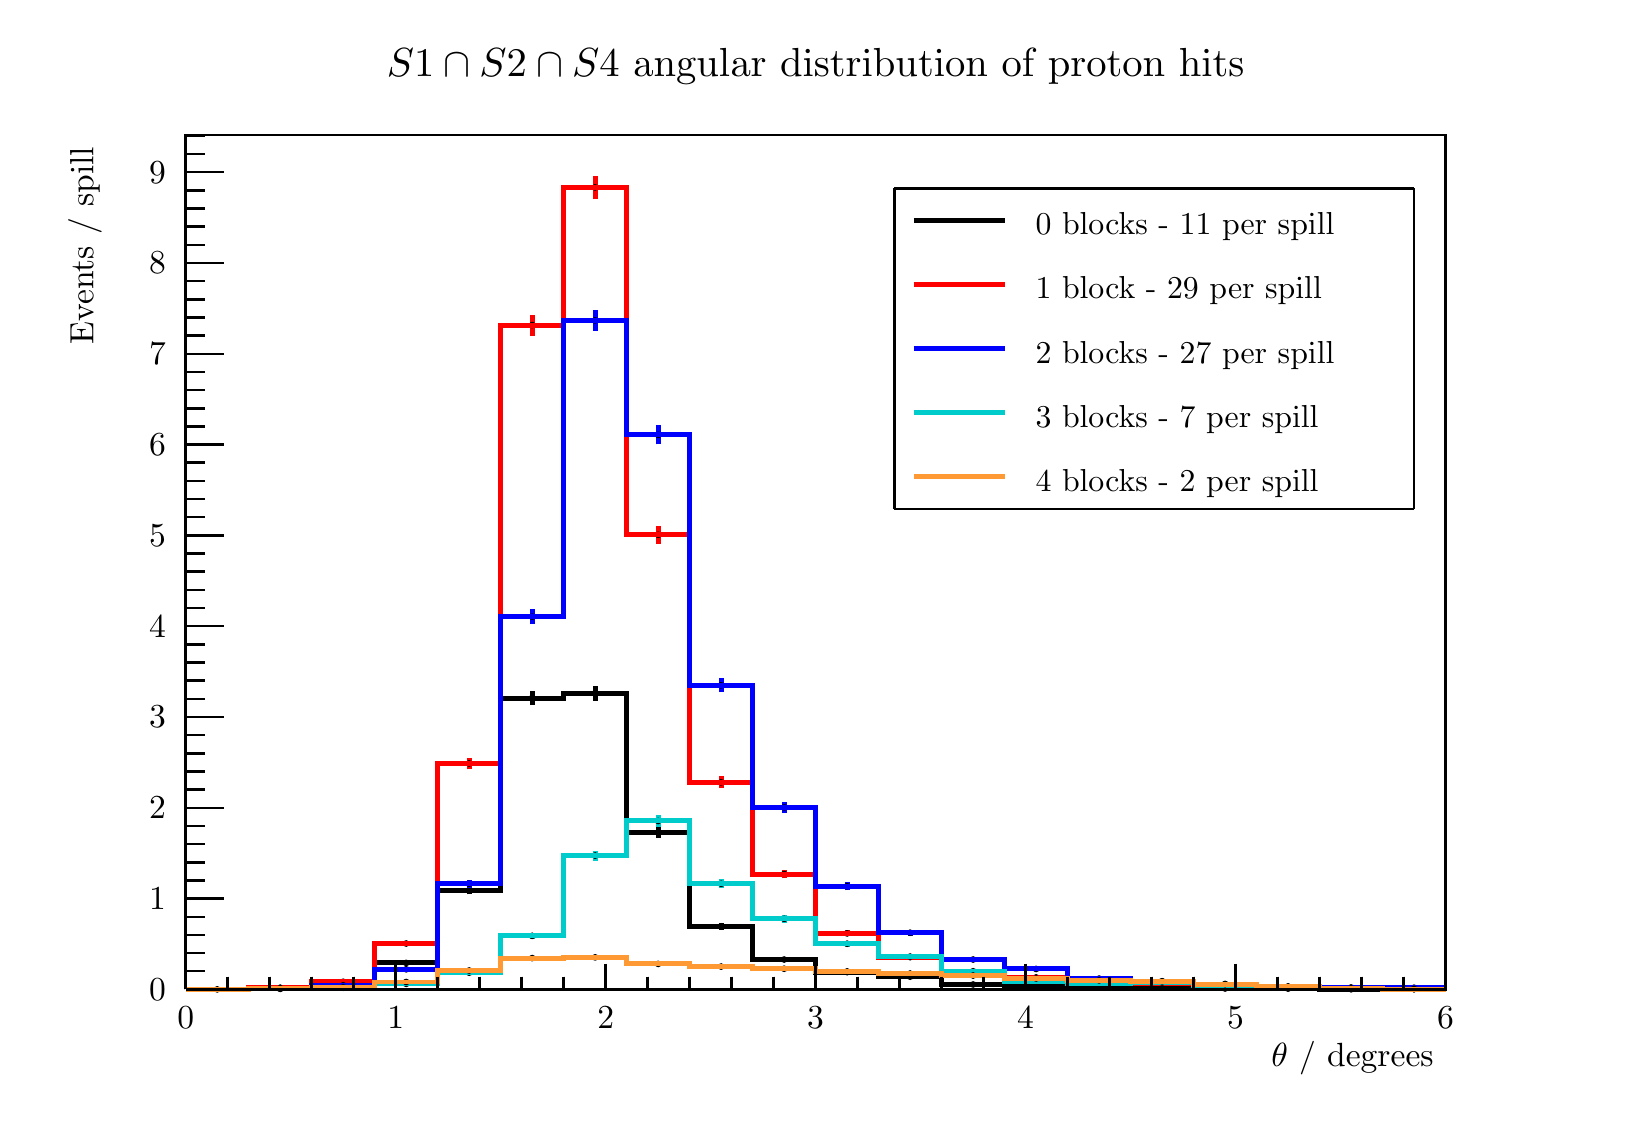
\begin{tikzpicture}
\pgfdeclareplotmark{cross} {
\pgfpathmoveto{\pgfpoint{-0.3\pgfplotmarksize}{\pgfplotmarksize}}
\pgfpathlineto{\pgfpoint{+0.3\pgfplotmarksize}{\pgfplotmarksize}}
\pgfpathlineto{\pgfpoint{+0.3\pgfplotmarksize}{0.3\pgfplotmarksize}}
\pgfpathlineto{\pgfpoint{+1\pgfplotmarksize}{0.3\pgfplotmarksize}}
\pgfpathlineto{\pgfpoint{+1\pgfplotmarksize}{-0.3\pgfplotmarksize}}
\pgfpathlineto{\pgfpoint{+0.3\pgfplotmarksize}{-0.3\pgfplotmarksize}}
\pgfpathlineto{\pgfpoint{+0.3\pgfplotmarksize}{-1.\pgfplotmarksize}}
\pgfpathlineto{\pgfpoint{-0.3\pgfplotmarksize}{-1.\pgfplotmarksize}}
\pgfpathlineto{\pgfpoint{-0.3\pgfplotmarksize}{-0.3\pgfplotmarksize}}
\pgfpathlineto{\pgfpoint{-1.\pgfplotmarksize}{-0.3\pgfplotmarksize}}
\pgfpathlineto{\pgfpoint{-1.\pgfplotmarksize}{0.3\pgfplotmarksize}}
\pgfpathlineto{\pgfpoint{-0.3\pgfplotmarksize}{0.3\pgfplotmarksize}}
\pgfpathclose
\pgfusepathqstroke
}
\pgfdeclareplotmark{cross*} {
\pgfpathmoveto{\pgfpoint{-0.3\pgfplotmarksize}{\pgfplotmarksize}}
\pgfpathlineto{\pgfpoint{+0.3\pgfplotmarksize}{\pgfplotmarksize}}
\pgfpathlineto{\pgfpoint{+0.3\pgfplotmarksize}{0.3\pgfplotmarksize}}
\pgfpathlineto{\pgfpoint{+1\pgfplotmarksize}{0.3\pgfplotmarksize}}
\pgfpathlineto{\pgfpoint{+1\pgfplotmarksize}{-0.3\pgfplotmarksize}}
\pgfpathlineto{\pgfpoint{+0.3\pgfplotmarksize}{-0.3\pgfplotmarksize}}
\pgfpathlineto{\pgfpoint{+0.3\pgfplotmarksize}{-1.\pgfplotmarksize}}
\pgfpathlineto{\pgfpoint{-0.3\pgfplotmarksize}{-1.\pgfplotmarksize}}
\pgfpathlineto{\pgfpoint{-0.3\pgfplotmarksize}{-0.3\pgfplotmarksize}}
\pgfpathlineto{\pgfpoint{-1.\pgfplotmarksize}{-0.3\pgfplotmarksize}}
\pgfpathlineto{\pgfpoint{-1.\pgfplotmarksize}{0.3\pgfplotmarksize}}
\pgfpathlineto{\pgfpoint{-0.3\pgfplotmarksize}{0.3\pgfplotmarksize}}
\pgfpathclose
\pgfusepathqfillstroke
}
\pgfdeclareplotmark{newstar} {
\pgfpathmoveto{\pgfqpoint{0pt}{\pgfplotmarksize}}
\pgfpathlineto{\pgfqpointpolar{44}{0.5\pgfplotmarksize}}
\pgfpathlineto{\pgfqpointpolar{18}{\pgfplotmarksize}}
\pgfpathlineto{\pgfqpointpolar{-20}{0.5\pgfplotmarksize}}
\pgfpathlineto{\pgfqpointpolar{-54}{\pgfplotmarksize}}
\pgfpathlineto{\pgfqpointpolar{-90}{0.5\pgfplotmarksize}}
\pgfpathlineto{\pgfqpointpolar{234}{\pgfplotmarksize}}
\pgfpathlineto{\pgfqpointpolar{198}{0.5\pgfplotmarksize}}
\pgfpathlineto{\pgfqpointpolar{162}{\pgfplotmarksize}}
\pgfpathlineto{\pgfqpointpolar{134}{0.5\pgfplotmarksize}}
\pgfpathclose
\pgfusepathqstroke
}
\pgfdeclareplotmark{newstar*} {
\pgfpathmoveto{\pgfqpoint{0pt}{\pgfplotmarksize}}
\pgfpathlineto{\pgfqpointpolar{44}{0.5\pgfplotmarksize}}
\pgfpathlineto{\pgfqpointpolar{18}{\pgfplotmarksize}}
\pgfpathlineto{\pgfqpointpolar{-20}{0.5\pgfplotmarksize}}
\pgfpathlineto{\pgfqpointpolar{-54}{\pgfplotmarksize}}
\pgfpathlineto{\pgfqpointpolar{-90}{0.5\pgfplotmarksize}}
\pgfpathlineto{\pgfqpointpolar{234}{\pgfplotmarksize}}
\pgfpathlineto{\pgfqpointpolar{198}{0.5\pgfplotmarksize}}
\pgfpathlineto{\pgfqpointpolar{162}{\pgfplotmarksize}}
\pgfpathlineto{\pgfqpointpolar{134}{0.5\pgfplotmarksize}}
\pgfpathclose
\pgfusepathqfillstroke
}
\definecolor{c}{rgb}{1,1,1};
\draw [color=c, fill=c] (0,0) rectangle (20,13.5632);
\draw [color=c, fill=c] (2,1.35632) rectangle (18,12.2069);
\definecolor{c}{rgb}{0,0,0};
\draw [c,line width=0.9] (2,1.35632) -- (2,12.2069) -- (18,12.2069) -- (18,1.35632) -- (2,1.35632);
\definecolor{c}{rgb}{1,1,1};
\draw [color=c, fill=c] (2,1.35632) rectangle (18,12.2069);
\definecolor{c}{rgb}{0,0,0};
\draw [c,line width=0.9] (2,1.35632) -- (2,12.2069) -- (18,12.2069) -- (18,1.35632) -- (2,1.35632);
\definecolor{c}{rgb}{0,0,0.6};
\draw [c,line width=0.9] (2,1.35632) -- (2.8,1.35632) -- (2.8,1.35632) -- (3.6,1.35632) -- (3.6,1.35632) -- (4.4,1.35632) -- (4.4,1.35632) -- (5.2,1.35632) -- (5.2,1.35632) -- (6,1.35632) -- (6,1.35632) -- (6.8,1.35632) -- (6.8,1.35632) --
 (7.6,1.35632) -- (7.6,1.35632) -- (8.4,1.35632) -- (8.4,1.35632) -- (9.2,1.35632) -- (9.2,1.35632) -- (10,1.35632) -- (10,1.35632) -- (10.8,1.35632) -- (10.8,1.35632) -- (11.6,1.35632) -- (11.6,1.35632) -- (12.4,1.35632) -- (12.4,1.35632) --
 (13.2,1.35632) -- (13.2,1.35632) -- (14,1.35632) -- (14,1.35632) -- (14.8,1.35632) -- (14.8,1.35632) -- (15.6,1.35632) -- (15.6,1.35632) -- (16.4,1.35632) -- (16.4,1.35632) -- (17.2,1.35632) -- (17.2,1.35632) -- (18,1.35632);
\definecolor{c}{rgb}{0,0,0};
\draw [c,line width=0.9] (2,1.35632) -- (18,1.35632);
\draw [anchor= east] (18,0.488276) node[scale=1.2126, color=c, rotate=0]{$\theta$ / degrees};
\draw [c,line width=0.9] (2,1.68184) -- (2,1.35632);
\draw [c,line width=0.9] (2.53333,1.51908) -- (2.53333,1.35632);
\draw [c,line width=0.9] (3.06667,1.51908) -- (3.06667,1.35632);
\draw [c,line width=0.9] (3.6,1.51908) -- (3.6,1.35632);
\draw [c,line width=0.9] (4.13333,1.51908) -- (4.13333,1.35632);
\draw [c,line width=0.9] (4.66667,1.68184) -- (4.66667,1.35632);
\draw [c,line width=0.9] (5.2,1.51908) -- (5.2,1.35632);
\draw [c,line width=0.9] (5.73333,1.51908) -- (5.73333,1.35632);
\draw [c,line width=0.9] (6.26667,1.51908) -- (6.26667,1.35632);
\draw [c,line width=0.9] (6.8,1.51908) -- (6.8,1.35632);
\draw [c,line width=0.9] (7.33333,1.68184) -- (7.33333,1.35632);
\draw [c,line width=0.9] (7.86667,1.51908) -- (7.86667,1.35632);
\draw [c,line width=0.9] (8.4,1.51908) -- (8.4,1.35632);
\draw [c,line width=0.9] (8.93333,1.51908) -- (8.93333,1.35632);
\draw [c,line width=0.9] (9.46667,1.51908) -- (9.46667,1.35632);
\draw [c,line width=0.9] (10,1.68184) -- (10,1.35632);
\draw [c,line width=0.9] (10.5333,1.51908) -- (10.5333,1.35632);
\draw [c,line width=0.9] (11.0667,1.51908) -- (11.0667,1.35632);
\draw [c,line width=0.9] (11.6,1.51908) -- (11.6,1.35632);
\draw [c,line width=0.9] (12.1333,1.51908) -- (12.1333,1.35632);
\draw [c,line width=0.9] (12.6667,1.68184) -- (12.6667,1.35632);
\draw [c,line width=0.9] (13.2,1.51908) -- (13.2,1.35632);
\draw [c,line width=0.9] (13.7333,1.51908) -- (13.7333,1.35632);
\draw [c,line width=0.9] (14.2667,1.51908) -- (14.2667,1.35632);
\draw [c,line width=0.9] (14.8,1.51908) -- (14.8,1.35632);
\draw [c,line width=0.9] (15.3333,1.68184) -- (15.3333,1.35632);
\draw [c,line width=0.9] (15.8667,1.51908) -- (15.8667,1.35632);
\draw [c,line width=0.9] (16.4,1.51908) -- (16.4,1.35632);
\draw [c,line width=0.9] (16.9333,1.51908) -- (16.9333,1.35632);
\draw [c,line width=0.9] (17.4667,1.51908) -- (17.4667,1.35632);
\draw [c,line width=0.9] (18,1.68184) -- (18,1.35632);
\draw [anchor=base] (2,0.854483) node[scale=1.2126, color=c, rotate=0]{0};
\draw [anchor=base] (4.66667,0.854483) node[scale=1.2126, color=c, rotate=0]{1};
\draw [anchor=base] (7.33333,0.854483) node[scale=1.2126, color=c, rotate=0]{2};
\draw [anchor=base] (10,0.854483) node[scale=1.2126, color=c, rotate=0]{3};
\draw [anchor=base] (12.6667,0.854483) node[scale=1.2126, color=c, rotate=0]{4};
\draw [anchor=base] (15.3333,0.854483) node[scale=1.2126, color=c, rotate=0]{5};
\draw [anchor=base] (18,0.854483) node[scale=1.2126, color=c, rotate=0]{6};
\draw [c,line width=0.9] (2,1.35632) -- (2,12.2069);
\draw [anchor= east] (0.72,12.2069) node[scale=1.2126, color=c, rotate=90]{ Events / spill};
\draw [c,line width=0.9] (2.48,1.35632) -- (2,1.35632);
\draw [c,line width=0.9] (2.24,1.58696) -- (2,1.58696);
\draw [c,line width=0.9] (2.24,1.81759) -- (2,1.81759);
\draw [c,line width=0.9] (2.24,2.04823) -- (2,2.04823);
\draw [c,line width=0.9] (2.24,2.27886) -- (2,2.27886);
\draw [c,line width=0.9] (2.48,2.5095) -- (2,2.5095);
\draw [c,line width=0.9] (2.24,2.74013) -- (2,2.74013);
\draw [c,line width=0.9] (2.24,2.97077) -- (2,2.97077);
\draw [c,line width=0.9] (2.24,3.20141) -- (2,3.20141);
\draw [c,line width=0.9] (2.24,3.43204) -- (2,3.43204);
\draw [c,line width=0.9] (2.48,3.66268) -- (2,3.66268);
\draw [c,line width=0.9] (2.24,3.89331) -- (2,3.89331);
\draw [c,line width=0.9] (2.24,4.12395) -- (2,4.12395);
\draw [c,line width=0.9] (2.24,4.35458) -- (2,4.35458);
\draw [c,line width=0.9] (2.24,4.58522) -- (2,4.58522);
\draw [c,line width=0.9] (2.48,4.81585) -- (2,4.81585);
\draw [c,line width=0.9] (2.24,5.04649) -- (2,5.04649);
\draw [c,line width=0.9] (2.24,5.27712) -- (2,5.27712);
\draw [c,line width=0.9] (2.24,5.50776) -- (2,5.50776);
\draw [c,line width=0.9] (2.24,5.7384) -- (2,5.7384);
\draw [c,line width=0.9] (2.48,5.96903) -- (2,5.96903);
\draw [c,line width=0.9] (2.24,6.19967) -- (2,6.19967);
\draw [c,line width=0.9] (2.24,6.4303) -- (2,6.4303);
\draw [c,line width=0.9] (2.24,6.66094) -- (2,6.66094);
\draw [c,line width=0.9] (2.24,6.89157) -- (2,6.89157);
\draw [c,line width=0.9] (2.48,7.12221) -- (2,7.12221);
\draw [c,line width=0.9] (2.24,7.35284) -- (2,7.35284);
\draw [c,line width=0.9] (2.24,7.58348) -- (2,7.58348);
\draw [c,line width=0.9] (2.24,7.81412) -- (2,7.81412);
\draw [c,line width=0.9] (2.24,8.04475) -- (2,8.04475);
\draw [c,line width=0.9] (2.48,8.27539) -- (2,8.27539);
\draw [c,line width=0.9] (2.24,8.50602) -- (2,8.50602);
\draw [c,line width=0.9] (2.24,8.73666) -- (2,8.73666);
\draw [c,line width=0.9] (2.24,8.96729) -- (2,8.96729);
\draw [c,line width=0.9] (2.24,9.19793) -- (2,9.19793);
\draw [c,line width=0.9] (2.48,9.42856) -- (2,9.42856);
\draw [c,line width=0.9] (2.24,9.6592) -- (2,9.6592);
\draw [c,line width=0.9] (2.24,9.88983) -- (2,9.88983);
\draw [c,line width=0.9] (2.24,10.1205) -- (2,10.1205);
\draw [c,line width=0.9] (2.24,10.3511) -- (2,10.3511);
\draw [c,line width=0.9] (2.48,10.5817) -- (2,10.5817);
\draw [c,line width=0.9] (2.24,10.8124) -- (2,10.8124);
\draw [c,line width=0.9] (2.24,11.043) -- (2,11.043);
\draw [c,line width=0.9] (2.24,11.2736) -- (2,11.2736);
\draw [c,line width=0.9] (2.24,11.5043) -- (2,11.5043);
\draw [c,line width=0.9] (2.48,11.7349) -- (2,11.7349);
\draw [c,line width=0.9] (2.48,11.7349) -- (2,11.7349);
\draw [c,line width=0.9] (2.24,11.9656) -- (2,11.9656);
\draw [c,line width=0.9] (2.24,12.1962) -- (2,12.1962);
\draw [anchor= east] (1.9,1.35632) node[scale=1.2126, color=c, rotate=0]{0};
\draw [anchor= east] (1.9,2.5095) node[scale=1.2126, color=c, rotate=0]{1};
\draw [anchor= east] (1.9,3.66268) node[scale=1.2126, color=c, rotate=0]{2};
\draw [anchor= east] (1.9,4.81585) node[scale=1.2126, color=c, rotate=0]{3};
\draw [anchor= east] (1.9,5.96903) node[scale=1.2126, color=c, rotate=0]{4};
\draw [anchor= east] (1.9,7.12221) node[scale=1.2126, color=c, rotate=0]{5};
\draw [anchor= east] (1.9,8.27539) node[scale=1.2126, color=c, rotate=0]{6};
\draw [anchor= east] (1.9,9.42856) node[scale=1.2126, color=c, rotate=0]{7};
\draw [anchor= east] (1.9,10.5817) node[scale=1.2126, color=c, rotate=0]{8};
\draw [anchor= east] (1.9,11.7349) node[scale=1.2126, color=c, rotate=0]{9};
\draw [c,line width=1.8] (3.2,1.36907) -- (3.2,1.3733);
\draw [c,line width=1.8] (3.2,1.3733) -- (3.2,1.37753);
\foreach \P in {(3.2,1.3733)}{\draw[mark options={color=c,fill=c},mark size=2.402402pt,mark=*,mark size=1pt] plot coordinates {\P};}
\draw [c,line width=1.8] (4,1.42823) -- (4,1.43742);
\draw [c,line width=1.8] (4,1.43742) -- (4,1.44661);
\foreach \P in {(4,1.43742)}{\draw[mark options={color=c,fill=c},mark size=2.402402pt,mark=*,mark size=1pt] plot coordinates {\P};}
\draw [c,line width=1.8] (4.8,1.67212) -- (4.8,1.6928);
\draw [c,line width=1.8] (4.8,1.6928) -- (4.8,1.71347);
\foreach \P in {(4.8,1.6928)}{\draw[mark options={color=c,fill=c},mark size=2.402402pt,mark=*,mark size=1pt] plot coordinates {\P};}
\draw [c,line width=1.8] (5.6,2.56355) -- (5.6,2.61121);
\draw [c,line width=1.8] (5.6,2.61121) -- (5.6,2.65886);
\foreach \P in {(5.6,2.61121)}{\draw[mark options={color=c,fill=c},mark size=2.402402pt,mark=*,mark size=1pt] plot coordinates {\P};}
\draw [c,line width=1.8] (6.4,4.96678) -- (6.4,5.05684);
\draw [c,line width=1.8] (6.4,5.05684) -- (6.4,5.14691);
\foreach \P in {(6.4,5.05684)}{\draw[mark options={color=c,fill=c},mark size=2.402402pt,mark=*,mark size=1pt] plot coordinates {\P};}
\draw [c,line width=1.8] (7.2,5.02241) -- (7.2,5.11701);
\draw [c,line width=1.8] (7.2,5.11701) -- (7.2,5.2116);
\foreach \P in {(7.2,5.11701)}{\draw[mark options={color=c,fill=c},mark size=2.402402pt,mark=*,mark size=1pt] plot coordinates {\P};}
\draw [c,line width=1.8] (8,3.28178) -- (8,3.34989);
\draw [c,line width=1.8] (8,3.34989) -- (8,3.41799);
\foreach \P in {(8,3.34989)}{\draw[mark options={color=c,fill=c},mark size=2.402402pt,mark=*,mark size=1pt] plot coordinates {\P};}
\draw [c,line width=1.8] (8.8,2.11628) -- (8.8,2.15828);
\draw [c,line width=1.8] (8.8,2.15828) -- (8.8,2.20028);
\foreach \P in {(8.8,2.15828)}{\draw[mark options={color=c,fill=c},mark size=2.402402pt,mark=*,mark size=1pt] plot coordinates {\P};}
\draw [c,line width=1.8] (9.6,1.70615) -- (9.6,1.7356);
\draw [c,line width=1.8] (9.6,1.7356) -- (9.6,1.76505);
\foreach \P in {(9.6,1.7356)}{\draw[mark options={color=c,fill=c},mark size=2.402402pt,mark=*,mark size=1pt] plot coordinates {\P};}
\draw [c,line width=1.8] (10.4,1.55295) -- (10.4,1.57505);
\draw [c,line width=1.8] (10.4,1.57505) -- (10.4,1.59714);
\foreach \P in {(10.4,1.57505)}{\draw[mark options={color=c,fill=c},mark size=2.402402pt,mark=*,mark size=1pt] plot coordinates {\P};}
\draw [c,line width=1.8] (11.2,1.49898) -- (11.2,1.51803);
\draw [c,line width=1.8] (11.2,1.51803) -- (11.2,1.53708);
\foreach \P in {(11.2,1.51803)}{\draw[mark options={color=c,fill=c},mark size=2.402402pt,mark=*,mark size=1pt] plot coordinates {\P};}
\draw [c,line width=1.8] (12,1.40758) -- (12,1.41881);
\draw [c,line width=1.8] (12,1.41881) -- (12,1.43005);
\foreach \P in {(12,1.41881)}{\draw[mark options={color=c,fill=c},mark size=2.402402pt,mark=*,mark size=1pt] plot coordinates {\P};}
\draw [c,line width=1.8] (12.8,1.39023) -- (12.8,1.39862);
\draw [c,line width=1.8] (12.8,1.39862) -- (12.8,1.40701);
\foreach \P in {(12.8,1.39862)}{\draw[mark options={color=c,fill=c},mark size=2.402402pt,mark=*,mark size=1pt] plot coordinates {\P};}
\draw [c,line width=1.8] (13.6,1.38187) -- (13.6,1.39153);
\draw [c,line width=1.8] (13.6,1.39153) -- (13.6,1.4012);
\foreach \P in {(13.6,1.39153)}{\draw[mark options={color=c,fill=c},mark size=2.402402pt,mark=*,mark size=1pt] plot coordinates {\P};}
\draw [c,line width=1.8] (14.4,1.37637) -- (14.4,1.3839);
\draw [c,line width=1.8] (14.4,1.3839) -- (14.4,1.39144);
\foreach \P in {(14.4,1.3839)}{\draw[mark options={color=c,fill=c},mark size=2.402402pt,mark=*,mark size=1pt] plot coordinates {\P};}
\draw [c,line width=1.8] (15.2,1.36247) -- (15.2,1.36751);
\draw [c,line width=1.8] (15.2,1.36751) -- (15.2,1.37255);
\foreach \P in {(15.2,1.36751)}{\draw[mark options={color=c,fill=c},mark size=2.402402pt,mark=*,mark size=1pt] plot coordinates {\P};}
\draw [c,line width=1.8] (16,1.36227) -- (16,1.366);
\draw [c,line width=1.8] (16,1.366) -- (16,1.36973);
\foreach \P in {(16,1.366)}{\draw[mark options={color=c,fill=c},mark size=2.402402pt,mark=*,mark size=1pt] plot coordinates {\P};}
\draw [c,line width=1.8] (16.8,1.35632) -- (16.8,1.35796);
\draw [c,line width=1.8] (16.8,1.35796) -- (16.8,1.35961);
\foreach \P in {(16.8,1.35796)}{\draw[mark options={color=c,fill=c},mark size=2.402402pt,mark=*,mark size=1pt] plot coordinates {\P};}
\draw [c,line width=1.8] (17.6,1.35632) -- (17.6,1.36005);
\draw [c,line width=1.8] (17.6,1.36005) -- (17.6,1.36378);
\foreach \P in {(17.6,1.36005)}{\draw[mark options={color=c,fill=c},mark size=2.402402pt,mark=*,mark size=1pt] plot coordinates {\P};}
\draw [c,line width=1.8] (2,1.35632) -- (2.8,1.35632) -- (2.8,1.3733) -- (3.6,1.3733) -- (3.6,1.43742) -- (4.4,1.43742) -- (4.4,1.6928) -- (5.2,1.6928) -- (5.2,2.61121) -- (6,2.61121) -- (6,5.05684) -- (6.8,5.05684) -- (6.8,5.11701) -- (7.6,5.11701)
 -- (7.6,3.34989) -- (8.4,3.34989) -- (8.4,2.15828) -- (9.2,2.15828) -- (9.2,1.7356) -- (10,1.7356) -- (10,1.57505) -- (10.8,1.57505) -- (10.8,1.51803) -- (11.6,1.51803) -- (11.6,1.41881) -- (12.4,1.41881) -- (12.4,1.39862) -- (13.2,1.39862) --
 (13.2,1.39153) -- (14,1.39153) -- (14,1.3839) -- (14.8,1.3839) -- (14.8,1.36751) -- (15.6,1.36751) -- (15.6,1.366) -- (16.4,1.366) -- (16.4,1.35796) -- (17.2,1.35796) -- (17.2,1.36005) -- (18,1.36005);
\definecolor{c}{rgb}{1,0,0};
\draw [c,line width=1.8] (3.2,1.37162) -- (3.2,1.37796);
\draw [c,line width=1.8] (3.2,1.37796) -- (3.2,1.38429);
\definecolor{c}{rgb}{0,0,0};
\foreach \P in {(3.2,1.37796)}{\draw[mark options={color=c,fill=c},mark size=2.402402pt,mark=*,mark size=1pt] plot coordinates {\P};}
\definecolor{c}{rgb}{1,0,0};
\draw [c,line width=1.8] (4,1.44099) -- (4,1.45349);
\draw [c,line width=1.8] (4,1.45349) -- (4,1.466);
\definecolor{c}{rgb}{0,0,0};
\foreach \P in {(4,1.45349)}{\draw[mark options={color=c,fill=c},mark size=2.402402pt,mark=*,mark size=1pt] plot coordinates {\P};}
\definecolor{c}{rgb}{1,0,0};
\draw [c,line width=1.8] (4.8,1.90595) -- (4.8,1.93895);
\draw [c,line width=1.8] (4.8,1.93895) -- (4.8,1.97196);
\definecolor{c}{rgb}{0,0,0};
\foreach \P in {(4.8,1.93895)}{\draw[mark options={color=c,fill=c},mark size=2.402402pt,mark=*,mark size=1pt] plot coordinates {\P};}
\definecolor{c}{rgb}{1,0,0};
\draw [c,line width=1.8] (5.6,4.15112) -- (5.6,4.22584);
\draw [c,line width=1.8] (5.6,4.22584) -- (5.6,4.30055);
\definecolor{c}{rgb}{0,0,0};
\foreach \P in {(5.6,4.22584)}{\draw[mark options={color=c,fill=c},mark size=2.402402pt,mark=*,mark size=1pt] plot coordinates {\P};}
\definecolor{c}{rgb}{1,0,0};
\draw [c,line width=1.8] (6.4,9.65938) -- (6.4,9.79309);
\draw [c,line width=1.8] (6.4,9.79309) -- (6.4,9.92681);
\definecolor{c}{rgb}{0,0,0};
\foreach \P in {(6.4,9.79309)}{\draw[mark options={color=c,fill=c},mark size=2.402402pt,mark=*,mark size=1pt] plot coordinates {\P};}
\definecolor{c}{rgb}{1,0,0};
\draw [c,line width=1.8] (7.2,11.392) -- (7.2,11.5411);
\draw [c,line width=1.8] (7.2,11.5411) -- (7.2,11.6902);
\definecolor{c}{rgb}{0,0,0};
\foreach \P in {(7.2,11.5411)}{\draw[mark options={color=c,fill=c},mark size=2.402402pt,mark=*,mark size=1pt] plot coordinates {\P};}
\definecolor{c}{rgb}{1,0,0};
\draw [c,line width=1.8] (8,7.01779) -- (8,7.12997);
\draw [c,line width=1.8] (8,7.12997) -- (8,7.24215);
\definecolor{c}{rgb}{0,0,0};
\foreach \P in {(8,7.12997)}{\draw[mark options={color=c,fill=c},mark size=2.402402pt,mark=*,mark size=1pt] plot coordinates {\P};}
\definecolor{c}{rgb}{1,0,0};
\draw [c,line width=1.8] (8.8,3.91124) -- (8.8,3.98602);
\draw [c,line width=1.8] (8.8,3.98602) -- (8.8,4.0608);
\definecolor{c}{rgb}{0,0,0};
\foreach \P in {(8.8,3.98602)}{\draw[mark options={color=c,fill=c},mark size=2.402402pt,mark=*,mark size=1pt] plot coordinates {\P};}
\definecolor{c}{rgb}{1,0,0};
\draw [c,line width=1.8] (9.6,2.76618) -- (9.6,2.82168);
\draw [c,line width=1.8] (9.6,2.82168) -- (9.6,2.87719);
\definecolor{c}{rgb}{0,0,0};
\foreach \P in {(9.6,2.82168)}{\draw[mark options={color=c,fill=c},mark size=2.402402pt,mark=*,mark size=1pt] plot coordinates {\P};}
\definecolor{c}{rgb}{1,0,0};
\draw [c,line width=1.8] (10.4,2.02843) -- (10.4,2.06711);
\draw [c,line width=1.8] (10.4,2.06711) -- (10.4,2.1058);
\definecolor{c}{rgb}{0,0,0};
\foreach \P in {(10.4,2.06711)}{\draw[mark options={color=c,fill=c},mark size=2.402402pt,mark=*,mark size=1pt] plot coordinates {\P};}
\definecolor{c}{rgb}{1,0,0};
\draw [c,line width=1.8] (11.2,1.73628) -- (11.2,1.76561);
\draw [c,line width=1.8] (11.2,1.76561) -- (11.2,1.79495);
\definecolor{c}{rgb}{0,0,0};
\foreach \P in {(11.2,1.76561)}{\draw[mark options={color=c,fill=c},mark size=2.402402pt,mark=*,mark size=1pt] plot coordinates {\P};}
\definecolor{c}{rgb}{1,0,0};
\draw [c,line width=1.8] (12,1.5353) -- (12,1.55634);
\draw [c,line width=1.8] (12,1.55634) -- (12,1.57739);
\definecolor{c}{rgb}{0,0,0};
\foreach \P in {(12,1.55634)}{\draw[mark options={color=c,fill=c},mark size=2.402402pt,mark=*,mark size=1pt] plot coordinates {\P};}
\definecolor{c}{rgb}{1,0,0};
\draw [c,line width=1.8] (12.8,1.49073) -- (12.8,1.50855);
\draw [c,line width=1.8] (12.8,1.50855) -- (12.8,1.52638);
\definecolor{c}{rgb}{0,0,0};
\foreach \P in {(12.8,1.50855)}{\draw[mark options={color=c,fill=c},mark size=2.402402pt,mark=*,mark size=1pt] plot coordinates {\P};}
\definecolor{c}{rgb}{1,0,0};
\draw [c,line width=1.8] (13.6,1.47258) -- (13.6,1.48978);
\draw [c,line width=1.8] (13.6,1.48978) -- (13.6,1.50697);
\definecolor{c}{rgb}{0,0,0};
\foreach \P in {(13.6,1.48978)}{\draw[mark options={color=c,fill=c},mark size=2.402402pt,mark=*,mark size=1pt] plot coordinates {\P};}
\definecolor{c}{rgb}{1,0,0};
\draw [c,line width=1.8] (14.4,1.4201) -- (14.4,1.43303);
\draw [c,line width=1.8] (14.4,1.43303) -- (14.4,1.44596);
\definecolor{c}{rgb}{0,0,0};
\foreach \P in {(14.4,1.43303)}{\draw[mark options={color=c,fill=c},mark size=2.402402pt,mark=*,mark size=1pt] plot coordinates {\P};}
\definecolor{c}{rgb}{1,0,0};
\draw [c,line width=1.8] (15.2,1.38109) -- (15.2,1.389);
\draw [c,line width=1.8] (15.2,1.389) -- (15.2,1.39691);
\definecolor{c}{rgb}{0,0,0};
\foreach \P in {(15.2,1.389)}{\draw[mark options={color=c,fill=c},mark size=2.402402pt,mark=*,mark size=1pt] plot coordinates {\P};}
\definecolor{c}{rgb}{1,0,0};
\draw [c,line width=1.8] (16,1.37467) -- (16,1.38246);
\draw [c,line width=1.8] (16,1.38246) -- (16,1.39025);
\definecolor{c}{rgb}{0,0,0};
\foreach \P in {(16,1.38246)}{\draw[mark options={color=c,fill=c},mark size=2.402402pt,mark=*,mark size=1pt] plot coordinates {\P};}
\definecolor{c}{rgb}{1,0,0};
\draw [c,line width=1.8] (16.8,1.36157) -- (16.8,1.36627);
\draw [c,line width=1.8] (16.8,1.36627) -- (16.8,1.37098);
\definecolor{c}{rgb}{0,0,0};
\foreach \P in {(16.8,1.36627)}{\draw[mark options={color=c,fill=c},mark size=2.402402pt,mark=*,mark size=1pt] plot coordinates {\P};}
\definecolor{c}{rgb}{1,0,0};
\draw [c,line width=1.8] (2,1.35632) -- (2.8,1.35632) -- (2.8,1.37796) -- (3.6,1.37796) -- (3.6,1.45349) -- (4.4,1.45349) -- (4.4,1.93895) -- (5.2,1.93895) -- (5.2,4.22584) -- (6,4.22584) -- (6,9.79309) -- (6.8,9.79309) -- (6.8,11.5411) --
 (7.6,11.5411) -- (7.6,7.12997) -- (8.4,7.12997) -- (8.4,3.98602) -- (9.2,3.98602) -- (9.2,2.82168) -- (10,2.82168) -- (10,2.06711) -- (10.8,2.06711) -- (10.8,1.76561) -- (11.6,1.76561) -- (11.6,1.55634) -- (12.4,1.55634) -- (12.4,1.50855) --
 (13.2,1.50855) -- (13.2,1.48978) -- (14,1.48978) -- (14,1.43303) -- (14.8,1.43303) -- (14.8,1.389) -- (15.6,1.389) -- (15.6,1.38246) -- (16.4,1.38246) -- (16.4,1.36627) -- (17.2,1.36627) -- (17.2,1.35632) -- (18,1.35632);
\definecolor{c}{rgb}{0,0,1};
\draw [c,line width=1.8] (3.2,1.36602) -- (3.2,1.37135);
\draw [c,line width=1.8] (3.2,1.37135) -- (3.2,1.37669);
\definecolor{c}{rgb}{0,0,0};
\foreach \P in {(3.2,1.37135)}{\draw[mark options={color=c,fill=c},mark size=2.402402pt,mark=*,mark size=1pt] plot coordinates {\P};}
\definecolor{c}{rgb}{0,0,1};
\draw [c,line width=1.8] (4,1.39968) -- (4,1.40866);
\draw [c,line width=1.8] (4,1.40866) -- (4,1.41764);
\definecolor{c}{rgb}{0,0,0};
\foreach \P in {(4,1.40866)}{\draw[mark options={color=c,fill=c},mark size=2.402402pt,mark=*,mark size=1pt] plot coordinates {\P};}
\definecolor{c}{rgb}{0,0,1};
\draw [c,line width=1.8] (4.8,1.59071) -- (4.8,1.61147);
\draw [c,line width=1.8] (4.8,1.61147) -- (4.8,1.63223);
\definecolor{c}{rgb}{0,0,0};
\foreach \P in {(4.8,1.61147)}{\draw[mark options={color=c,fill=c},mark size=2.402402pt,mark=*,mark size=1pt] plot coordinates {\P};}
\definecolor{c}{rgb}{0,0,1};
\draw [c,line width=1.8] (5.6,2.64778) -- (5.6,2.69632);
\draw [c,line width=1.8] (5.6,2.69632) -- (5.6,2.74486);
\definecolor{c}{rgb}{0,0,0};
\foreach \P in {(5.6,2.69632)}{\draw[mark options={color=c,fill=c},mark size=2.402402pt,mark=*,mark size=1pt] plot coordinates {\P};}
\definecolor{c}{rgb}{0,0,1};
\draw [c,line width=1.8] (6.4,5.99525) -- (6.4,6.08958);
\draw [c,line width=1.8] (6.4,6.08958) -- (6.4,6.18392);
\definecolor{c}{rgb}{0,0,0};
\foreach \P in {(6.4,6.08958)}{\draw[mark options={color=c,fill=c},mark size=2.402402pt,mark=*,mark size=1pt] plot coordinates {\P};}
\definecolor{c}{rgb}{0,0,1};
\draw [c,line width=1.8] (7.2,9.72165) -- (7.2,9.85277);
\draw [c,line width=1.8] (7.2,9.85277) -- (7.2,9.98388);
\definecolor{c}{rgb}{0,0,0};
\foreach \P in {(7.2,9.85277)}{\draw[mark options={color=c,fill=c},mark size=2.402402pt,mark=*,mark size=1pt] plot coordinates {\P};}
\definecolor{c}{rgb}{0,0,1};
\draw [c,line width=1.8] (8,8.27773) -- (8,8.39895);
\draw [c,line width=1.8] (8,8.39895) -- (8,8.52017);
\definecolor{c}{rgb}{0,0,0};
\foreach \P in {(8,8.39895)}{\draw[mark options={color=c,fill=c},mark size=2.402402pt,mark=*,mark size=1pt] plot coordinates {\P};}
\definecolor{c}{rgb}{0,0,1};
\draw [c,line width=1.8] (8.8,5.1306) -- (8.8,5.21872);
\draw [c,line width=1.8] (8.8,5.21872) -- (8.8,5.30685);
\definecolor{c}{rgb}{0,0,0};
\foreach \P in {(8.8,5.21872)}{\draw[mark options={color=c,fill=c},mark size=2.402402pt,mark=*,mark size=1pt] plot coordinates {\P};}
\definecolor{c}{rgb}{0,0,1};
\draw [c,line width=1.8] (9.6,3.59935) -- (9.6,3.6676);
\draw [c,line width=1.8] (9.6,3.6676) -- (9.6,3.73585);
\definecolor{c}{rgb}{0,0,0};
\foreach \P in {(9.6,3.6676)}{\draw[mark options={color=c,fill=c},mark size=2.402402pt,mark=*,mark size=1pt] plot coordinates {\P};}
\definecolor{c}{rgb}{0,0,1};
\draw [c,line width=1.8] (10.4,2.61599) -- (10.4,2.66745);
\draw [c,line width=1.8] (10.4,2.66745) -- (10.4,2.71891);
\definecolor{c}{rgb}{0,0,0};
\foreach \P in {(10.4,2.66745)}{\draw[mark options={color=c,fill=c},mark size=2.402402pt,mark=*,mark size=1pt] plot coordinates {\P};}
\definecolor{c}{rgb}{0,0,1};
\draw [c,line width=1.8] (11.2,2.03802) -- (11.2,2.07642);
\draw [c,line width=1.8] (11.2,2.07642) -- (11.2,2.11483);
\definecolor{c}{rgb}{0,0,0};
\foreach \P in {(11.2,2.07642)}{\draw[mark options={color=c,fill=c},mark size=2.402402pt,mark=*,mark size=1pt] plot coordinates {\P};}
\definecolor{c}{rgb}{0,0,1};
\draw [c,line width=1.8] (12,1.70768) -- (12,1.73565);
\draw [c,line width=1.8] (12,1.73565) -- (12,1.76361);
\definecolor{c}{rgb}{0,0,0};
\foreach \P in {(12,1.73565)}{\draw[mark options={color=c,fill=c},mark size=2.402402pt,mark=*,mark size=1pt] plot coordinates {\P};}
\definecolor{c}{rgb}{0,0,1};
\draw [c,line width=1.8] (12.8,1.59297) -- (12.8,1.61596);
\draw [c,line width=1.8] (12.8,1.61596) -- (12.8,1.63896);
\definecolor{c}{rgb}{0,0,0};
\foreach \P in {(12.8,1.61596)}{\draw[mark options={color=c,fill=c},mark size=2.402402pt,mark=*,mark size=1pt] plot coordinates {\P};}
\definecolor{c}{rgb}{0,0,1};
\draw [c,line width=1.8] (13.6,1.47604) -- (13.6,1.49308);
\draw [c,line width=1.8] (13.6,1.49308) -- (13.6,1.51011);
\definecolor{c}{rgb}{0,0,0};
\foreach \P in {(13.6,1.49308)}{\draw[mark options={color=c,fill=c},mark size=2.402402pt,mark=*,mark size=1pt] plot coordinates {\P};}
\definecolor{c}{rgb}{0,0,1};
\draw [c,line width=1.8] (14.4,1.44567) -- (14.4,1.46005);
\draw [c,line width=1.8] (14.4,1.46005) -- (14.4,1.47444);
\definecolor{c}{rgb}{0,0,0};
\foreach \P in {(14.4,1.46005)}{\draw[mark options={color=c,fill=c},mark size=2.402402pt,mark=*,mark size=1pt] plot coordinates {\P};}
\definecolor{c}{rgb}{0,0,1};
\draw [c,line width=1.8] (15.2,1.41305) -- (15.2,1.42495);
\draw [c,line width=1.8] (15.2,1.42495) -- (15.2,1.43686);
\definecolor{c}{rgb}{0,0,0};
\foreach \P in {(15.2,1.42495)}{\draw[mark options={color=c,fill=c},mark size=2.402402pt,mark=*,mark size=1pt] plot coordinates {\P};}
\definecolor{c}{rgb}{0,0,1};
\draw [c,line width=1.8] (16,1.37605) -- (16,1.38313);
\draw [c,line width=1.8] (16,1.38313) -- (16,1.39021);
\definecolor{c}{rgb}{0,0,0};
\foreach \P in {(16,1.38313)}{\draw[mark options={color=c,fill=c},mark size=2.402402pt,mark=*,mark size=1pt] plot coordinates {\P};}
\definecolor{c}{rgb}{0,0,1};
\draw [c,line width=1.8] (16.8,1.37376) -- (16.8,1.38092);
\draw [c,line width=1.8] (16.8,1.38092) -- (16.8,1.38807);
\definecolor{c}{rgb}{0,0,0};
\foreach \P in {(16.8,1.38092)}{\draw[mark options={color=c,fill=c},mark size=2.402402pt,mark=*,mark size=1pt] plot coordinates {\P};}
\definecolor{c}{rgb}{0,0,1};
\draw [c,line width=1.8] (17.6,1.37086) -- (17.6,1.37792);
\draw [c,line width=1.8] (17.6,1.37792) -- (17.6,1.38497);
\definecolor{c}{rgb}{0,0,0};
\foreach \P in {(17.6,1.37792)}{\draw[mark options={color=c,fill=c},mark size=2.402402pt,mark=*,mark size=1pt] plot coordinates {\P};}
\definecolor{c}{rgb}{0,0,1};
\draw [c,line width=1.8] (2,1.35632) -- (2.8,1.35632) -- (2.8,1.37135) -- (3.6,1.37135) -- (3.6,1.40866) -- (4.4,1.40866) -- (4.4,1.61147) -- (5.2,1.61147) -- (5.2,2.69632) -- (6,2.69632) -- (6,6.08958) -- (6.8,6.08958) -- (6.8,9.85277) --
 (7.6,9.85277) -- (7.6,8.39895) -- (8.4,8.39895) -- (8.4,5.21872) -- (9.2,5.21872) -- (9.2,3.6676) -- (10,3.6676) -- (10,2.66745) -- (10.8,2.66745) -- (10.8,2.07642) -- (11.6,2.07642) -- (11.6,1.73565) -- (12.4,1.73565) -- (12.4,1.61596) --
 (13.2,1.61596) -- (13.2,1.49308) -- (14,1.49308) -- (14,1.46005) -- (14.8,1.46005) -- (14.8,1.42495) -- (15.6,1.42495) -- (15.6,1.38313) -- (16.4,1.38313) -- (16.4,1.38092) -- (17.2,1.38092) -- (17.2,1.37792) -- (18,1.37792);
\definecolor{c}{rgb}{0,0.8,0.8};
\draw [c,line width=1.8] (3.2,1.36119) -- (3.2,1.36578);
\draw [c,line width=1.8] (3.2,1.36578) -- (3.2,1.37037);
\definecolor{c}{rgb}{0,0,0};
\foreach \P in {(3.2,1.36578)}{\draw[mark options={color=c,fill=c},mark size=2.402402pt,mark=*,mark size=1pt] plot coordinates {\P};}
\definecolor{c}{rgb}{0,0.8,0.8};
\draw [c,line width=1.8] (4,1.37046) -- (4,1.37758);
\draw [c,line width=1.8] (4,1.37758) -- (4,1.3847);
\definecolor{c}{rgb}{0,0,0};
\foreach \P in {(4,1.37758)}{\draw[mark options={color=c,fill=c},mark size=2.402402pt,mark=*,mark size=1pt] plot coordinates {\P};}
\definecolor{c}{rgb}{0,0.8,0.8};
\draw [c,line width=1.8] (4.8,1.41388) -- (4.8,1.42652);
\draw [c,line width=1.8] (4.8,1.42652) -- (4.8,1.43915);
\definecolor{c}{rgb}{0,0,0};
\foreach \P in {(4.8,1.42652)}{\draw[mark options={color=c,fill=c},mark size=2.402402pt,mark=*,mark size=1pt] plot coordinates {\P};}
\definecolor{c}{rgb}{0,0.8,0.8};
\draw [c,line width=1.8] (5.6,1.54618) -- (5.6,1.5683);
\draw [c,line width=1.8] (5.6,1.5683) -- (5.6,1.59042);
\definecolor{c}{rgb}{0,0,0};
\foreach \P in {(5.6,1.5683)}{\draw[mark options={color=c,fill=c},mark size=2.402402pt,mark=*,mark size=1pt] plot coordinates {\P};}
\definecolor{c}{rgb}{0,0.8,0.8};
\draw [c,line width=1.8] (6.4,1.99746) -- (6.4,2.03657);
\draw [c,line width=1.8] (6.4,2.03657) -- (6.4,2.07567);
\definecolor{c}{rgb}{0,0,0};
\foreach \P in {(6.4,2.03657)}{\draw[mark options={color=c,fill=c},mark size=2.402402pt,mark=*,mark size=1pt] plot coordinates {\P};}
\definecolor{c}{rgb}{0,0.8,0.8};
\draw [c,line width=1.8] (7.2,2.99164) -- (7.2,3.05593);
\draw [c,line width=1.8] (7.2,3.05593) -- (7.2,3.12021);
\definecolor{c}{rgb}{0,0,0};
\foreach \P in {(7.2,3.05593)}{\draw[mark options={color=c,fill=c},mark size=2.402402pt,mark=*,mark size=1pt] plot coordinates {\P};}
\definecolor{c}{rgb}{0,0.8,0.8};
\draw [c,line width=1.8] (8,3.42171) -- (8,3.49548);
\draw [c,line width=1.8] (8,3.49548) -- (8,3.56925);
\definecolor{c}{rgb}{0,0,0};
\foreach \P in {(8,3.49548)}{\draw[mark options={color=c,fill=c},mark size=2.402402pt,mark=*,mark size=1pt] plot coordinates {\P};}
\definecolor{c}{rgb}{0,0.8,0.8};
\draw [c,line width=1.8] (8.8,2.63928) -- (8.8,2.69729);
\draw [c,line width=1.8] (8.8,2.69729) -- (8.8,2.75529);
\definecolor{c}{rgb}{0,0,0};
\foreach \P in {(8.8,2.69729)}{\draw[mark options={color=c,fill=c},mark size=2.402402pt,mark=*,mark size=1pt] plot coordinates {\P};}
\definecolor{c}{rgb}{0,0.8,0.8};
\draw [c,line width=1.8] (9.6,2.20541) -- (9.6,2.25207);
\draw [c,line width=1.8] (9.6,2.25207) -- (9.6,2.29874);
\definecolor{c}{rgb}{0,0,0};
\foreach \P in {(9.6,2.25207)}{\draw[mark options={color=c,fill=c},mark size=2.402402pt,mark=*,mark size=1pt] plot coordinates {\P};}
\definecolor{c}{rgb}{0,0.8,0.8};
\draw [c,line width=1.8] (10.4,1.89835) -- (10.4,1.93659);
\draw [c,line width=1.8] (10.4,1.93659) -- (10.4,1.97482);
\definecolor{c}{rgb}{0,0,0};
\foreach \P in {(10.4,1.93659)}{\draw[mark options={color=c,fill=c},mark size=2.402402pt,mark=*,mark size=1pt] plot coordinates {\P};}
\definecolor{c}{rgb}{0,0.8,0.8};
\draw [c,line width=1.8] (11.2,1.74069) -- (11.2,1.7732);
\draw [c,line width=1.8] (11.2,1.7732) -- (11.2,1.80571);
\definecolor{c}{rgb}{0,0,0};
\foreach \P in {(11.2,1.7732)}{\draw[mark options={color=c,fill=c},mark size=2.402402pt,mark=*,mark size=1pt] plot coordinates {\P};}
\definecolor{c}{rgb}{0,0.8,0.8};
\draw [c,line width=1.8] (12,1.56205) -- (12,1.58658);
\draw [c,line width=1.8] (12,1.58658) -- (12,1.61111);
\definecolor{c}{rgb}{0,0,0};
\foreach \P in {(12,1.58658)}{\draw[mark options={color=c,fill=c},mark size=2.402402pt,mark=*,mark size=1pt] plot coordinates {\P};}
\definecolor{c}{rgb}{0,0.8,0.8};
\draw [c,line width=1.8] (12.8,1.44034) -- (12.8,1.45586);
\draw [c,line width=1.8] (12.8,1.45586) -- (12.8,1.47138);
\definecolor{c}{rgb}{0,0,0};
\foreach \P in {(12.8,1.45586)}{\draw[mark options={color=c,fill=c},mark size=2.402402pt,mark=*,mark size=1pt] plot coordinates {\P};}
\definecolor{c}{rgb}{0,0.8,0.8};
\draw [c,line width=1.8] (13.6,1.42221) -- (13.6,1.43717);
\draw [c,line width=1.8] (13.6,1.43717) -- (13.6,1.45214);
\definecolor{c}{rgb}{0,0,0};
\foreach \P in {(13.6,1.43717)}{\draw[mark options={color=c,fill=c},mark size=2.402402pt,mark=*,mark size=1pt] plot coordinates {\P};}
\definecolor{c}{rgb}{0,0.8,0.8};
\draw [c,line width=1.8] (14.4,1.42785) -- (14.4,1.44282);
\draw [c,line width=1.8] (14.4,1.44282) -- (14.4,1.45779);
\definecolor{c}{rgb}{0,0,0};
\foreach \P in {(14.4,1.44282)}{\draw[mark options={color=c,fill=c},mark size=2.402402pt,mark=*,mark size=1pt] plot coordinates {\P};}
\definecolor{c}{rgb}{0,0.8,0.8};
\draw [c,line width=1.8] (15.2,1.38712) -- (15.2,1.39734);
\draw [c,line width=1.8] (15.2,1.39734) -- (15.2,1.40757);
\definecolor{c}{rgb}{0,0,0};
\foreach \P in {(15.2,1.39734)}{\draw[mark options={color=c,fill=c},mark size=2.402402pt,mark=*,mark size=1pt] plot coordinates {\P};}
\definecolor{c}{rgb}{0,0.8,0.8};
\draw [c,line width=1.8] (16,1.38189) -- (16,1.39167);
\draw [c,line width=1.8] (16,1.39167) -- (16,1.40145);
\definecolor{c}{rgb}{0,0,0};
\foreach \P in {(16,1.39167)}{\draw[mark options={color=c,fill=c},mark size=2.402402pt,mark=*,mark size=1pt] plot coordinates {\P};}
\definecolor{c}{rgb}{0,0.8,0.8};
\draw [c,line width=1.8] (16.8,1.35923) -- (16.8,1.36352);
\draw [c,line width=1.8] (16.8,1.36352) -- (16.8,1.3678);
\definecolor{c}{rgb}{0,0,0};
\foreach \P in {(16.8,1.36352)}{\draw[mark options={color=c,fill=c},mark size=2.402402pt,mark=*,mark size=1pt] plot coordinates {\P};}
\definecolor{c}{rgb}{0,0.8,0.8};
\draw [c,line width=1.8] (17.6,1.35756) -- (17.6,1.36105);
\draw [c,line width=1.8] (17.6,1.36105) -- (17.6,1.36454);
\definecolor{c}{rgb}{0,0,0};
\foreach \P in {(17.6,1.36105)}{\draw[mark options={color=c,fill=c},mark size=2.402402pt,mark=*,mark size=1pt] plot coordinates {\P};}
\definecolor{c}{rgb}{0,0.8,0.8};
\draw [c,line width=1.8] (2,1.35632) -- (2.8,1.35632) -- (2.8,1.36578) -- (3.6,1.36578) -- (3.6,1.37758) -- (4.4,1.37758) -- (4.4,1.42652) -- (5.2,1.42652) -- (5.2,1.5683) -- (6,1.5683) -- (6,2.03657) -- (6.8,2.03657) -- (6.8,3.05593) --
 (7.6,3.05593) -- (7.6,3.49548) -- (8.4,3.49548) -- (8.4,2.69729) -- (9.2,2.69729) -- (9.2,2.25207) -- (10,2.25207) -- (10,1.93659) -- (10.8,1.93659) -- (10.8,1.7732) -- (11.6,1.7732) -- (11.6,1.58658) -- (12.4,1.58658) -- (12.4,1.45586) --
 (13.2,1.45586) -- (13.2,1.43717) -- (14,1.43717) -- (14,1.44282) -- (14.8,1.44282) -- (14.8,1.39734) -- (15.6,1.39734) -- (15.6,1.39167) -- (16.4,1.39167) -- (16.4,1.36352) -- (17.2,1.36352) -- (17.2,1.36105) -- (18,1.36105);
\definecolor{c}{rgb}{1,0.6,0.2};
\draw [c,line width=1.8] (2.4,1.35632) -- (2.4,1.35649);
\draw [c,line width=1.8] (2.4,1.35649) -- (2.4,1.35665);
\definecolor{c}{rgb}{0,0,0};
\foreach \P in {(2.4,1.35649)}{\draw[mark options={color=c,fill=c},mark size=2.402402pt,mark=*,mark size=1pt] plot coordinates {\P};}
\definecolor{c}{rgb}{1,0.6,0.2};
\draw [c,line width=1.8] (3.2,1.36192) -- (3.2,1.36289);
\draw [c,line width=1.8] (3.2,1.36289) -- (3.2,1.36385);
\definecolor{c}{rgb}{0,0,0};
\foreach \P in {(3.2,1.36289)}{\draw[mark options={color=c,fill=c},mark size=2.402402pt,mark=*,mark size=1pt] plot coordinates {\P};}
\definecolor{c}{rgb}{1,0.6,0.2};
\draw [c,line width=1.8] (4,1.37987) -- (4,1.38165);
\draw [c,line width=1.8] (4,1.38165) -- (4,1.38342);
\definecolor{c}{rgb}{0,0,0};
\foreach \P in {(4,1.38165)}{\draw[mark options={color=c,fill=c},mark size=2.402402pt,mark=*,mark size=1pt] plot coordinates {\P};}
\definecolor{c}{rgb}{1,0.6,0.2};
\draw [c,line width=1.8] (4.8,1.44676) -- (4.8,1.45031);
\draw [c,line width=1.8] (4.8,1.45031) -- (4.8,1.45387);
\definecolor{c}{rgb}{0,0,0};
\foreach \P in {(4.8,1.45031)}{\draw[mark options={color=c,fill=c},mark size=2.402402pt,mark=*,mark size=1pt] plot coordinates {\P};}
\definecolor{c}{rgb}{1,0.6,0.2};
\draw [c,line width=1.8] (5.6,1.59048) -- (5.6,1.59631);
\draw [c,line width=1.8] (5.6,1.59631) -- (5.6,1.60215);
\definecolor{c}{rgb}{0,0,0};
\foreach \P in {(5.6,1.59631)}{\draw[mark options={color=c,fill=c},mark size=2.402402pt,mark=*,mark size=1pt] plot coordinates {\P};}
\definecolor{c}{rgb}{1,0.6,0.2};
\draw [c,line width=1.8] (6.4,1.74617) -- (6.4,1.75387);
\draw [c,line width=1.8] (6.4,1.75387) -- (6.4,1.76157);
\definecolor{c}{rgb}{0,0,0};
\foreach \P in {(6.4,1.75387)}{\draw[mark options={color=c,fill=c},mark size=2.402402pt,mark=*,mark size=1pt] plot coordinates {\P};}
\definecolor{c}{rgb}{1,0.6,0.2};
\draw [c,line width=1.8] (7.2,1.75517) -- (7.2,1.76304);
\draw [c,line width=1.8] (7.2,1.76304) -- (7.2,1.77091);
\definecolor{c}{rgb}{0,0,0};
\foreach \P in {(7.2,1.76304)}{\draw[mark options={color=c,fill=c},mark size=2.402402pt,mark=*,mark size=1pt] plot coordinates {\P};}
\definecolor{c}{rgb}{1,0.6,0.2};
\draw [c,line width=1.8] (8,1.67328) -- (8,1.6803);
\draw [c,line width=1.8] (8,1.6803) -- (8,1.68731);
\definecolor{c}{rgb}{0,0,0};
\foreach \P in {(8,1.6803)}{\draw[mark options={color=c,fill=c},mark size=2.402402pt,mark=*,mark size=1pt] plot coordinates {\P};}
\definecolor{c}{rgb}{1,0.6,0.2};
\draw [c,line width=1.8] (8.8,1.63969) -- (8.8,1.64624);
\draw [c,line width=1.8] (8.8,1.64624) -- (8.8,1.6528);
\definecolor{c}{rgb}{0,0,0};
\foreach \P in {(8.8,1.64624)}{\draw[mark options={color=c,fill=c},mark size=2.402402pt,mark=*,mark size=1pt] plot coordinates {\P};}
\definecolor{c}{rgb}{1,0.6,0.2};
\draw [c,line width=1.8] (9.6,1.61245) -- (9.6,1.61868);
\draw [c,line width=1.8] (9.6,1.61868) -- (9.6,1.62491);
\definecolor{c}{rgb}{0,0,0};
\foreach \P in {(9.6,1.61868)}{\draw[mark options={color=c,fill=c},mark size=2.402402pt,mark=*,mark size=1pt] plot coordinates {\P};}
\definecolor{c}{rgb}{1,0.6,0.2};
\draw [c,line width=1.8] (10.4,1.57878) -- (10.4,1.58458);
\draw [c,line width=1.8] (10.4,1.58458) -- (10.4,1.59038);
\definecolor{c}{rgb}{0,0,0};
\foreach \P in {(10.4,1.58458)}{\draw[mark options={color=c,fill=c},mark size=2.402402pt,mark=*,mark size=1pt] plot coordinates {\P};}
\definecolor{c}{rgb}{1,0.6,0.2};
\draw [c,line width=1.8] (11.2,1.55196) -- (11.2,1.55741);
\draw [c,line width=1.8] (11.2,1.55741) -- (11.2,1.56285);
\definecolor{c}{rgb}{0,0,0};
\foreach \P in {(11.2,1.55741)}{\draw[mark options={color=c,fill=c},mark size=2.402402pt,mark=*,mark size=1pt] plot coordinates {\P};}
\definecolor{c}{rgb}{1,0.6,0.2};
\draw [c,line width=1.8] (12,1.52709) -- (12,1.53219);
\draw [c,line width=1.8] (12,1.53219) -- (12,1.53729);
\definecolor{c}{rgb}{0,0,0};
\foreach \P in {(12,1.53219)}{\draw[mark options={color=c,fill=c},mark size=2.402402pt,mark=*,mark size=1pt] plot coordinates {\P};}
\definecolor{c}{rgb}{1,0.6,0.2};
\draw [c,line width=1.8] (12.8,1.49061) -- (12.8,1.49509);
\draw [c,line width=1.8] (12.8,1.49509) -- (12.8,1.49958);
\definecolor{c}{rgb}{0,0,0};
\foreach \P in {(12.8,1.49509)}{\draw[mark options={color=c,fill=c},mark size=2.402402pt,mark=*,mark size=1pt] plot coordinates {\P};}
\definecolor{c}{rgb}{1,0.6,0.2};
\draw [c,line width=1.8] (13.6,1.46661) -- (13.6,1.47071);
\draw [c,line width=1.8] (13.6,1.47071) -- (13.6,1.47481);
\definecolor{c}{rgb}{0,0,0};
\foreach \P in {(13.6,1.47071)}{\draw[mark options={color=c,fill=c},mark size=2.402402pt,mark=*,mark size=1pt] plot coordinates {\P};}
\definecolor{c}{rgb}{1,0.6,0.2};
\draw [c,line width=1.8] (14.4,1.45433) -- (14.4,1.45819);
\draw [c,line width=1.8] (14.4,1.45819) -- (14.4,1.46205);
\definecolor{c}{rgb}{0,0,0};
\foreach \P in {(14.4,1.45819)}{\draw[mark options={color=c,fill=c},mark size=2.402402pt,mark=*,mark size=1pt] plot coordinates {\P};}
\definecolor{c}{rgb}{1,0.6,0.2};
\draw [c,line width=1.8] (15.2,1.41923) -- (15.2,1.42231);
\draw [c,line width=1.8] (15.2,1.42231) -- (15.2,1.42539);
\definecolor{c}{rgb}{0,0,0};
\foreach \P in {(15.2,1.42231)}{\draw[mark options={color=c,fill=c},mark size=2.402402pt,mark=*,mark size=1pt] plot coordinates {\P};}
\definecolor{c}{rgb}{1,0.6,0.2};
\draw [c,line width=1.8] (16,1.39062) -- (16,1.39291);
\draw [c,line width=1.8] (16,1.39291) -- (16,1.39519);
\definecolor{c}{rgb}{0,0,0};
\foreach \P in {(16,1.39291)}{\draw[mark options={color=c,fill=c},mark size=2.402402pt,mark=*,mark size=1pt] plot coordinates {\P};}
\definecolor{c}{rgb}{1,0.6,0.2};
\draw [c,line width=1.8] (16.8,1.36854) -- (16.8,1.3699);
\draw [c,line width=1.8] (16.8,1.3699) -- (16.8,1.37127);
\definecolor{c}{rgb}{0,0,0};
\foreach \P in {(16.8,1.3699)}{\draw[mark options={color=c,fill=c},mark size=2.402402pt,mark=*,mark size=1pt] plot coordinates {\P};}
\definecolor{c}{rgb}{1,0.6,0.2};
\draw [c,line width=1.8] (17.6,1.36031) -- (17.6,1.36113);
\draw [c,line width=1.8] (17.6,1.36113) -- (17.6,1.36196);
\definecolor{c}{rgb}{0,0,0};
\foreach \P in {(17.6,1.36113)}{\draw[mark options={color=c,fill=c},mark size=2.402402pt,mark=*,mark size=1pt] plot coordinates {\P};}
\definecolor{c}{rgb}{1,0.6,0.2};
\draw [c,line width=1.8] (2,1.35632) -- (2.8,1.35632) -- (2.8,1.36289) -- (3.6,1.36289) -- (3.6,1.38165) -- (4.4,1.38165) -- (4.4,1.45031) -- (5.2,1.45031) -- (5.2,1.59631) -- (6,1.59631) -- (6,1.75387) -- (6.8,1.75387) -- (6.8,1.76304) --
 (7.6,1.76304) -- (7.6,1.6803) -- (8.4,1.6803) -- (8.4,1.64624) -- (9.2,1.64624) -- (9.2,1.61868) -- (10,1.61868) -- (10,1.58458) -- (10.8,1.58458) -- (10.8,1.55741) -- (11.6,1.55741) -- (11.6,1.53219) -- (12.4,1.53219) -- (12.4,1.49509) --
 (13.2,1.49509) -- (13.2,1.47071) -- (14,1.47071) -- (14,1.45819) -- (14.8,1.45819) -- (14.8,1.42231) -- (15.6,1.42231) -- (15.6,1.39291) -- (16.4,1.39291) -- (16.4,1.3699) -- (17.2,1.3699) -- (17.2,1.36113) -- (18,1.36113);
\definecolor{c}{rgb}{0,0,0};
\draw [c,line width=0.9] (2,1.35632) -- (18,1.35632);
\draw [c,line width=0.9] (2,1.68184) -- (2,1.35632);
\draw [c,line width=0.9] (2.53333,1.51908) -- (2.53333,1.35632);
\draw [c,line width=0.9] (3.06667,1.51908) -- (3.06667,1.35632);
\draw [c,line width=0.9] (3.6,1.51908) -- (3.6,1.35632);
\draw [c,line width=0.9] (4.13333,1.51908) -- (4.13333,1.35632);
\draw [c,line width=0.9] (4.66667,1.68184) -- (4.66667,1.35632);
\draw [c,line width=0.9] (5.2,1.51908) -- (5.2,1.35632);
\draw [c,line width=0.9] (5.73333,1.51908) -- (5.73333,1.35632);
\draw [c,line width=0.9] (6.26667,1.51908) -- (6.26667,1.35632);
\draw [c,line width=0.9] (6.8,1.51908) -- (6.8,1.35632);
\draw [c,line width=0.9] (7.33333,1.68184) -- (7.33333,1.35632);
\draw [c,line width=0.9] (7.86667,1.51908) -- (7.86667,1.35632);
\draw [c,line width=0.9] (8.4,1.51908) -- (8.4,1.35632);
\draw [c,line width=0.9] (8.93333,1.51908) -- (8.93333,1.35632);
\draw [c,line width=0.9] (9.46667,1.51908) -- (9.46667,1.35632);
\draw [c,line width=0.9] (10,1.68184) -- (10,1.35632);
\draw [c,line width=0.9] (10.5333,1.51908) -- (10.5333,1.35632);
\draw [c,line width=0.9] (11.0667,1.51908) -- (11.0667,1.35632);
\draw [c,line width=0.9] (11.6,1.51908) -- (11.6,1.35632);
\draw [c,line width=0.9] (12.1333,1.51908) -- (12.1333,1.35632);
\draw [c,line width=0.9] (12.6667,1.68184) -- (12.6667,1.35632);
\draw [c,line width=0.9] (13.2,1.51908) -- (13.2,1.35632);
\draw [c,line width=0.9] (13.7333,1.51908) -- (13.7333,1.35632);
\draw [c,line width=0.9] (14.2667,1.51908) -- (14.2667,1.35632);
\draw [c,line width=0.9] (14.8,1.51908) -- (14.8,1.35632);
\draw [c,line width=0.9] (15.3333,1.68184) -- (15.3333,1.35632);
\draw [c,line width=0.9] (15.8667,1.51908) -- (15.8667,1.35632);
\draw [c,line width=0.9] (16.4,1.51908) -- (16.4,1.35632);
\draw [c,line width=0.9] (16.9333,1.51908) -- (16.9333,1.35632);
\draw [c,line width=0.9] (17.4667,1.51908) -- (17.4667,1.35632);
\draw [c,line width=0.9] (18,1.68184) -- (18,1.35632);
\draw [c,line width=0.9] (2,1.35632) -- (2,12.2069);
\draw [c,line width=0.9] (2.48,1.35632) -- (2,1.35632);
\draw [c,line width=0.9] (2.24,1.58696) -- (2,1.58696);
\draw [c,line width=0.9] (2.24,1.81759) -- (2,1.81759);
\draw [c,line width=0.9] (2.24,2.04823) -- (2,2.04823);
\draw [c,line width=0.9] (2.24,2.27886) -- (2,2.27886);
\draw [c,line width=0.9] (2.48,2.5095) -- (2,2.5095);
\draw [c,line width=0.9] (2.24,2.74013) -- (2,2.74013);
\draw [c,line width=0.9] (2.24,2.97077) -- (2,2.97077);
\draw [c,line width=0.9] (2.24,3.20141) -- (2,3.20141);
\draw [c,line width=0.9] (2.24,3.43204) -- (2,3.43204);
\draw [c,line width=0.9] (2.48,3.66268) -- (2,3.66268);
\draw [c,line width=0.9] (2.24,3.89331) -- (2,3.89331);
\draw [c,line width=0.9] (2.24,4.12395) -- (2,4.12395);
\draw [c,line width=0.9] (2.24,4.35458) -- (2,4.35458);
\draw [c,line width=0.9] (2.24,4.58522) -- (2,4.58522);
\draw [c,line width=0.9] (2.48,4.81585) -- (2,4.81585);
\draw [c,line width=0.9] (2.24,5.04649) -- (2,5.04649);
\draw [c,line width=0.9] (2.24,5.27712) -- (2,5.27712);
\draw [c,line width=0.9] (2.24,5.50776) -- (2,5.50776);
\draw [c,line width=0.9] (2.24,5.7384) -- (2,5.7384);
\draw [c,line width=0.9] (2.48,5.96903) -- (2,5.96903);
\draw [c,line width=0.9] (2.24,6.19967) -- (2,6.19967);
\draw [c,line width=0.9] (2.24,6.4303) -- (2,6.4303);
\draw [c,line width=0.9] (2.24,6.66094) -- (2,6.66094);
\draw [c,line width=0.9] (2.24,6.89157) -- (2,6.89157);
\draw [c,line width=0.9] (2.48,7.12221) -- (2,7.12221);
\draw [c,line width=0.9] (2.24,7.35284) -- (2,7.35284);
\draw [c,line width=0.9] (2.24,7.58348) -- (2,7.58348);
\draw [c,line width=0.9] (2.24,7.81412) -- (2,7.81412);
\draw [c,line width=0.9] (2.24,8.04475) -- (2,8.04475);
\draw [c,line width=0.9] (2.48,8.27539) -- (2,8.27539);
\draw [c,line width=0.9] (2.24,8.50602) -- (2,8.50602);
\draw [c,line width=0.9] (2.24,8.73666) -- (2,8.73666);
\draw [c,line width=0.9] (2.24,8.96729) -- (2,8.96729);
\draw [c,line width=0.9] (2.24,9.19793) -- (2,9.19793);
\draw [c,line width=0.9] (2.48,9.42856) -- (2,9.42856);
\draw [c,line width=0.9] (2.24,9.6592) -- (2,9.6592);
\draw [c,line width=0.9] (2.24,9.88983) -- (2,9.88983);
\draw [c,line width=0.9] (2.24,10.1205) -- (2,10.1205);
\draw [c,line width=0.9] (2.24,10.3511) -- (2,10.3511);
\draw [c,line width=0.9] (2.48,10.5817) -- (2,10.5817);
\draw [c,line width=0.9] (2.24,10.8124) -- (2,10.8124);
\draw [c,line width=0.9] (2.24,11.043) -- (2,11.043);
\draw [c,line width=0.9] (2.24,11.2736) -- (2,11.2736);
\draw [c,line width=0.9] (2.24,11.5043) -- (2,11.5043);
\draw [c,line width=0.9] (2.48,11.7349) -- (2,11.7349);
\draw [c,line width=0.9] (2.48,11.7349) -- (2,11.7349);
\draw [c,line width=0.9] (2.24,11.9656) -- (2,11.9656);
\draw [c,line width=0.9] (2.24,12.1962) -- (2,12.1962);
\draw (10,13.0816) node[scale=1.46788, color=c, rotate=0]{$S1 \cap S2 \cap S4$ angular distribution of proton hits};
\definecolor{c}{rgb}{1,1,1};
\draw [color=c, fill=c] (11,7.45977) rectangle (17.6,11.5287);
\definecolor{c}{rgb}{0,0,0};
\draw [c,line width=0.9] (11,7.45977) -- (17.6,7.45977);
\draw [c,line width=0.9] (17.6,7.45977) -- (17.6,11.5287);
\draw [c,line width=0.9] (17.6,11.5287) -- (11,11.5287);
\draw [c,line width=0.9] (11,11.5287) -- (11,7.45977);
\draw [anchor=base west] (12.65,10.9387) node[scale=1.14878, color=c, rotate=0]{0 blocks - 11 per spill};
\draw [c,line width=1.8] (11.2475,11.1218) -- (12.4025,11.1218);
\draw [anchor=base west] (12.65,10.1249) node[scale=1.14878, color=c, rotate=0]{1 block - 29 per spill};
\definecolor{c}{rgb}{1,0,0};
\draw [c,line width=1.8] (11.2475,10.308) -- (12.4025,10.308);
\definecolor{c}{rgb}{0,0,0};
\draw [anchor=base west] (12.65,9.31115) node[scale=1.14878, color=c, rotate=0]{2 blocks - 27 per spill};
\definecolor{c}{rgb}{0,0,1};
\draw [c,line width=1.8] (11.2475,9.49425) -- (12.4025,9.49425);
\definecolor{c}{rgb}{0,0,0};
\draw [anchor=base west] (12.65,8.49736) node[scale=1.14878, color=c, rotate=0]{3 blocks - 7 per spill};
\definecolor{c}{rgb}{0,0.8,0.8};
\draw [c,line width=1.8] (11.2475,8.68046) -- (12.4025,8.68046);
\definecolor{c}{rgb}{0,0,0};
\draw [anchor=base west] (12.65,7.68356) node[scale=1.14878, color=c, rotate=0]{4 blocks - 2 per spill};
\definecolor{c}{rgb}{1,0.6,0.2};
\draw [c,line width=1.8] (11.2475,7.86667) -- (12.4025,7.86667);
\end{tikzpicture}

	   		\end{adjustbox}
   			\caption{Distribution of hits identified in $S4$ as protons as a function of the number of moderator blocks and the horizontal off-axis angle, as measured from $S1$.}
   			\label{fig:thetas4pro}
   		\end{minipage} 
   		%\begin{minipage}[t]{0.48\textwidth}
   		%	\centering
   		%	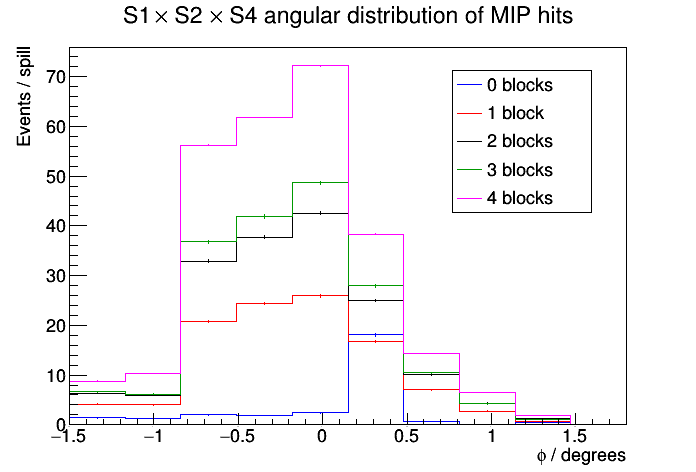
\includegraphics[width=\textwidth]{files/Figures/piS4Vert}
   		%	\caption{Distribution of hits identified in $S_{4}$ as minimum ionizing particles as a function of the number of moderator blocks and the vertical off-axis angle, as measured from $S_{1}$.}
   		%\end{minipage}
   		%\hspace{0.3cm}
   		%\begin{minipage}[t]{0.48\textwidth}
   		%	\centering
   		%	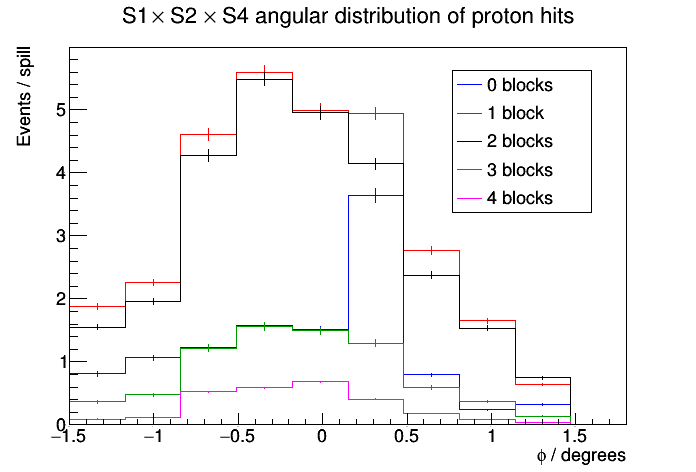
\includegraphics[width=\textwidth]{files/Figures/proS4Vert}
   		%	\caption{Distribution of hits identified in $S_{4}$ as protons as a function of the number of moderator blocks and the vertical off-axis angle, as measured from $S_{1}$.}
   		%\end{minipage}
	\end{figure}	
        
     Figures~\ref{fig:propiratio_s4_horz} and~\ref{fig:propiratio_s4_vert} show the ratio of protons to minimum ionizing particles as a function of the number of moderator blocks and the two off-axis angles.
     For the 0, 1 and 2 moderator block configurations, figure~\ref{fig:propiratio_s4_horz} shows the ratio
     \begin{equation*}
     \frac{N_{protons}}{N_{MIPs}}
     \end{equation*}	
     reaching its peak at a value of $\theta$ of approximately $2^{\circ}$.
     It is clear that in the angular region of this peak, the ratio of protons to pions has been dramatically increased from the expected on axis value of 1:6 seen previously.
     With the addition of moderator blocks, the size of the peak reduces until, in the 3 block configuration, it is no longer visible. 
     For the 4 block configuration, the proton/MIP ratio appears to be close to 0 for most values of $\theta$ but rises slightly at large values.
     
     Similarly, figure~\ref{fig:propiratio_s4_vert} shows the proton/MIP ratio falling with the addition of moderator blocks.
     For the 0, 1, 2 and 3 block configurations the ratio appears to rise as the vertical off-axis angle ($\phi$) moves further away from $0^{\circ}$. 
     For the 4 block configuration, the value of the proton/MIP ratio is close to zero at all values of $\phi$.
     
   	\begin{figure}[ht]
   		\begin{minipage}[t]{0.48\textwidth}
   			\begin{adjustbox}{max totalsize={\textwidth}{.35\textheight}, center}
   				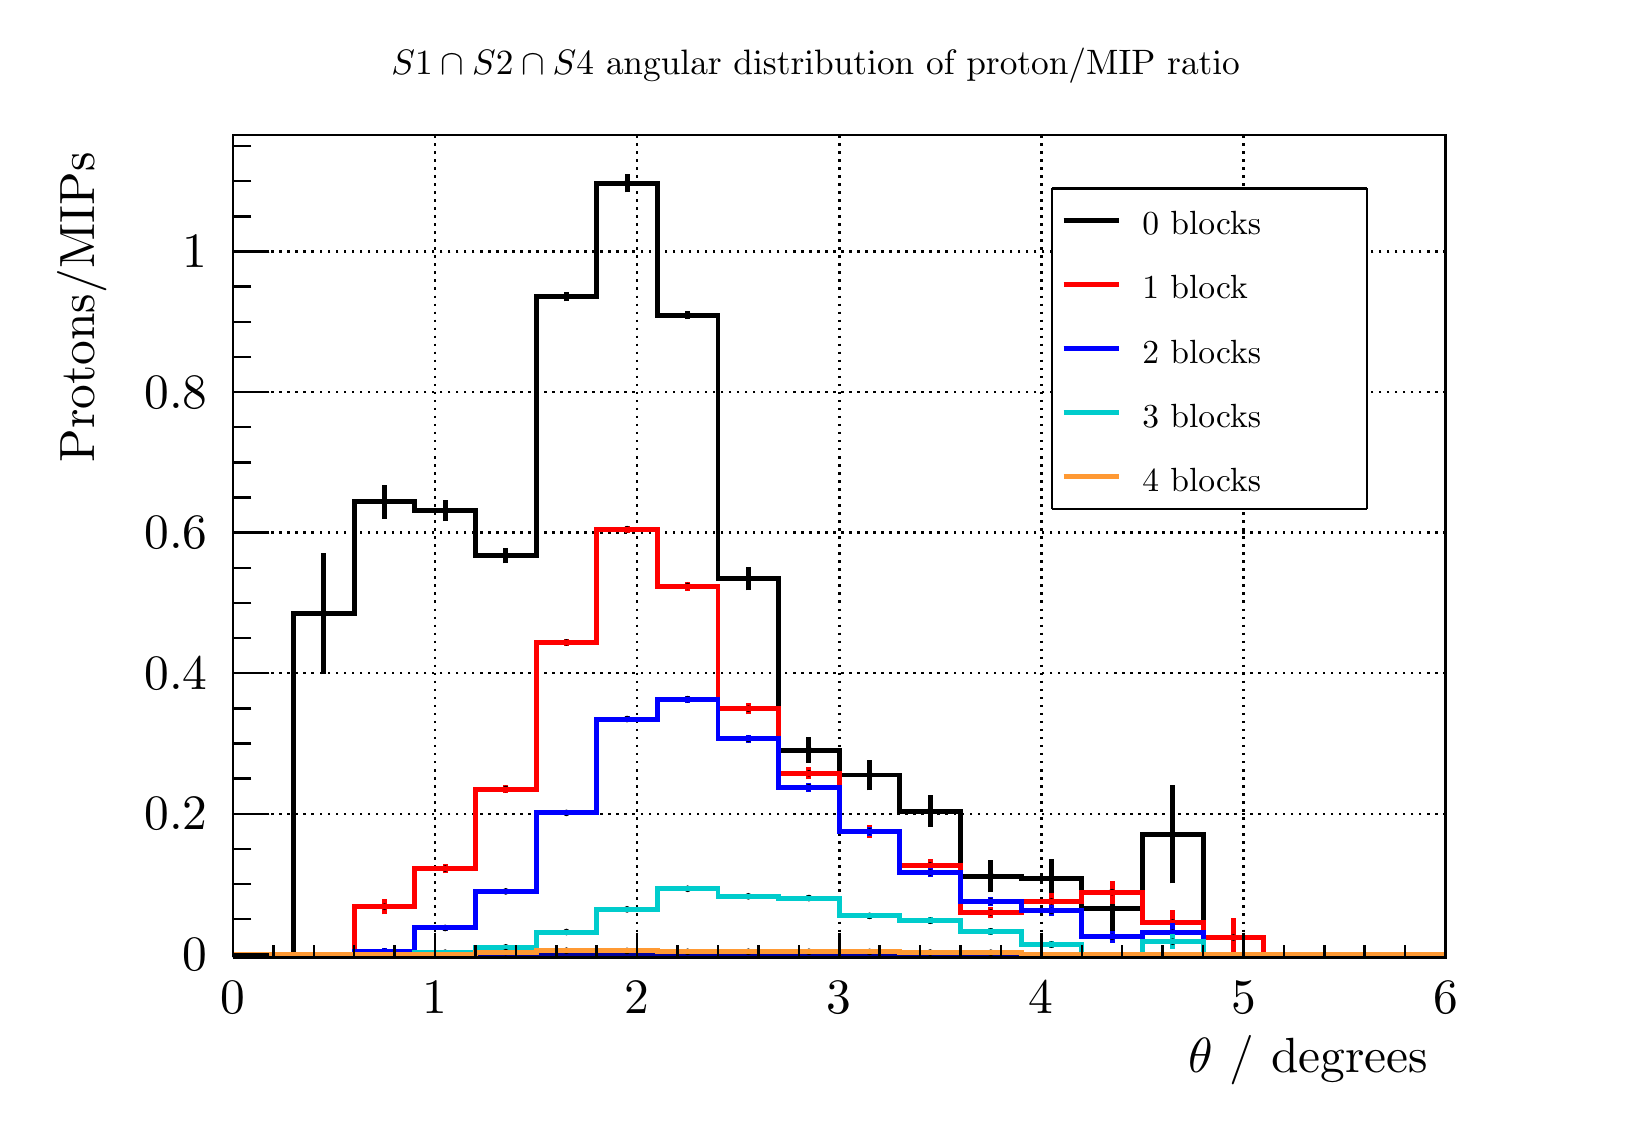
\begin{tikzpicture}
\pgfdeclareplotmark{cross} {
\pgfpathmoveto{\pgfpoint{-0.3\pgfplotmarksize}{\pgfplotmarksize}}
\pgfpathlineto{\pgfpoint{+0.3\pgfplotmarksize}{\pgfplotmarksize}}
\pgfpathlineto{\pgfpoint{+0.3\pgfplotmarksize}{0.3\pgfplotmarksize}}
\pgfpathlineto{\pgfpoint{+1\pgfplotmarksize}{0.3\pgfplotmarksize}}
\pgfpathlineto{\pgfpoint{+1\pgfplotmarksize}{-0.3\pgfplotmarksize}}
\pgfpathlineto{\pgfpoint{+0.3\pgfplotmarksize}{-0.3\pgfplotmarksize}}
\pgfpathlineto{\pgfpoint{+0.3\pgfplotmarksize}{-1.\pgfplotmarksize}}
\pgfpathlineto{\pgfpoint{-0.3\pgfplotmarksize}{-1.\pgfplotmarksize}}
\pgfpathlineto{\pgfpoint{-0.3\pgfplotmarksize}{-0.3\pgfplotmarksize}}
\pgfpathlineto{\pgfpoint{-1.\pgfplotmarksize}{-0.3\pgfplotmarksize}}
\pgfpathlineto{\pgfpoint{-1.\pgfplotmarksize}{0.3\pgfplotmarksize}}
\pgfpathlineto{\pgfpoint{-0.3\pgfplotmarksize}{0.3\pgfplotmarksize}}
\pgfpathclose
\pgfusepathqstroke
}
\pgfdeclareplotmark{cross*} {
\pgfpathmoveto{\pgfpoint{-0.3\pgfplotmarksize}{\pgfplotmarksize}}
\pgfpathlineto{\pgfpoint{+0.3\pgfplotmarksize}{\pgfplotmarksize}}
\pgfpathlineto{\pgfpoint{+0.3\pgfplotmarksize}{0.3\pgfplotmarksize}}
\pgfpathlineto{\pgfpoint{+1\pgfplotmarksize}{0.3\pgfplotmarksize}}
\pgfpathlineto{\pgfpoint{+1\pgfplotmarksize}{-0.3\pgfplotmarksize}}
\pgfpathlineto{\pgfpoint{+0.3\pgfplotmarksize}{-0.3\pgfplotmarksize}}
\pgfpathlineto{\pgfpoint{+0.3\pgfplotmarksize}{-1.\pgfplotmarksize}}
\pgfpathlineto{\pgfpoint{-0.3\pgfplotmarksize}{-1.\pgfplotmarksize}}
\pgfpathlineto{\pgfpoint{-0.3\pgfplotmarksize}{-0.3\pgfplotmarksize}}
\pgfpathlineto{\pgfpoint{-1.\pgfplotmarksize}{-0.3\pgfplotmarksize}}
\pgfpathlineto{\pgfpoint{-1.\pgfplotmarksize}{0.3\pgfplotmarksize}}
\pgfpathlineto{\pgfpoint{-0.3\pgfplotmarksize}{0.3\pgfplotmarksize}}
\pgfpathclose
\pgfusepathqfillstroke
}
\pgfdeclareplotmark{newstar} {
\pgfpathmoveto{\pgfqpoint{0pt}{\pgfplotmarksize}}
\pgfpathlineto{\pgfqpointpolar{44}{0.5\pgfplotmarksize}}
\pgfpathlineto{\pgfqpointpolar{18}{\pgfplotmarksize}}
\pgfpathlineto{\pgfqpointpolar{-20}{0.5\pgfplotmarksize}}
\pgfpathlineto{\pgfqpointpolar{-54}{\pgfplotmarksize}}
\pgfpathlineto{\pgfqpointpolar{-90}{0.5\pgfplotmarksize}}
\pgfpathlineto{\pgfqpointpolar{234}{\pgfplotmarksize}}
\pgfpathlineto{\pgfqpointpolar{198}{0.5\pgfplotmarksize}}
\pgfpathlineto{\pgfqpointpolar{162}{\pgfplotmarksize}}
\pgfpathlineto{\pgfqpointpolar{134}{0.5\pgfplotmarksize}}
\pgfpathclose
\pgfusepathqstroke
}
\pgfdeclareplotmark{newstar*} {
\pgfpathmoveto{\pgfqpoint{0pt}{\pgfplotmarksize}}
\pgfpathlineto{\pgfqpointpolar{44}{0.5\pgfplotmarksize}}
\pgfpathlineto{\pgfqpointpolar{18}{\pgfplotmarksize}}
\pgfpathlineto{\pgfqpointpolar{-20}{0.5\pgfplotmarksize}}
\pgfpathlineto{\pgfqpointpolar{-54}{\pgfplotmarksize}}
\pgfpathlineto{\pgfqpointpolar{-90}{0.5\pgfplotmarksize}}
\pgfpathlineto{\pgfqpointpolar{234}{\pgfplotmarksize}}
\pgfpathlineto{\pgfqpointpolar{198}{0.5\pgfplotmarksize}}
\pgfpathlineto{\pgfqpointpolar{162}{\pgfplotmarksize}}
\pgfpathlineto{\pgfqpointpolar{134}{0.5\pgfplotmarksize}}
\pgfpathclose
\pgfusepathqfillstroke
}
\definecolor{c}{rgb}{1,1,1};
\draw [color=c, fill=c] (0,0) rectangle (20,13.5632);
\draw [color=c, fill=c] (2.6,1.76322) rectangle (18,12.2069);
\definecolor{c}{rgb}{0,0,0};
\draw [c,line width=0.9] (2.6,1.76322) -- (2.6,12.2069) -- (18,12.2069) -- (18,1.76322) -- (2.6,1.76322);
\definecolor{c}{rgb}{1,1,1};
\draw [color=c, fill=c] (2.6,1.76322) rectangle (18,12.2069);
\definecolor{c}{rgb}{0,0,0};
\draw [c,line width=0.9] (2.6,1.76322) -- (2.6,12.2069) -- (18,12.2069) -- (18,1.76322) -- (2.6,1.76322);
\draw [c,line width=0.9] (2.6,1.76322) -- (18,1.76322);
\draw [c,dotted,line width=0.9] (2.6,12.2069) -- (2.6,1.76322);
\draw [c,dotted,line width=0.9] (5.16667,12.2069) -- (5.16667,1.76322);
\draw [c,dotted,line width=0.9] (7.73333,12.2069) -- (7.73333,1.76322);
\draw [c,dotted,line width=0.9] (10.3,12.2069) -- (10.3,1.76322);
\draw [c,dotted,line width=0.9] (12.8667,12.2069) -- (12.8667,1.76322);
\draw [c,dotted,line width=0.9] (15.4333,12.2069) -- (15.4333,1.76322);
\draw [c,dotted,line width=0.9] (18,12.2069) -- (18,1.76322);
\draw [c,line width=0.9] (2.6,1.76322) -- (2.6,12.2069);
\draw [c,dotted,line width=0.9] (18,1.80099) -- (2.6,1.80099);
\draw [c,dotted,line width=0.9] (18,3.58635) -- (2.6,3.58635);
\draw [c,dotted,line width=0.9] (18,5.37171) -- (2.6,5.37171);
\draw [c,dotted,line width=0.9] (18,7.15707) -- (2.6,7.15707);
\draw [c,dotted,line width=0.9] (18,8.94243) -- (2.6,8.94243);
\draw [c,dotted,line width=0.9] (18,10.7278) -- (2.6,10.7278);
\draw [c,dotted,line width=0.9] (18,1.80099) -- (2.6,1.80099);
\draw [c,dotted,line width=0.9] (18,10.7278) -- (2.6,10.7278);
\definecolor{c}{rgb}{0,0,0.6};
\draw [c,line width=0.9] (2.6,1.80099) -- (3.37,1.80099) -- (3.37,1.80099) -- (4.14,1.80099) -- (4.14,1.80099) -- (4.91,1.80099) -- (4.91,1.80099) -- (5.68,1.80099) -- (5.68,1.80099) -- (6.45,1.80099) -- (6.45,1.80099) -- (7.22,1.80099) --
 (7.22,1.80099) -- (7.99,1.80099) -- (7.99,1.80099) -- (8.76,1.80099) -- (8.76,1.80099) -- (9.53,1.80099) -- (9.53,1.80099) -- (10.3,1.80099) -- (10.3,1.80099) -- (11.07,1.80099) -- (11.07,1.80099) -- (11.84,1.80099) -- (11.84,1.80099) --
 (12.61,1.80099) -- (12.61,1.80099) -- (13.38,1.80099) -- (13.38,1.80099) -- (14.15,1.80099) -- (14.15,1.80099) -- (14.92,1.80099) -- (14.92,1.80099) -- (15.69,1.80099) -- (15.69,1.80099) -- (16.46,1.80099) -- (16.46,1.80099) -- (17.23,1.80099) --
 (17.23,1.80099) -- (18,1.80099);
\definecolor{c}{rgb}{0,0,0};
\draw [c,line width=0.9] (2.6,1.76322) -- (18,1.76322);
\draw [anchor= east] (18,0.461149) node[scale=1.78699, color=c, rotate=0]{$\theta$ / degrees};
\draw [c,line width=0.9] (2.6,2.07653) -- (2.6,1.76322);
\draw [c,line width=0.9] (3.11333,1.91987) -- (3.11333,1.76322);
\draw [c,line width=0.9] (3.62667,1.91987) -- (3.62667,1.76322);
\draw [c,line width=0.9] (4.14,1.91987) -- (4.14,1.76322);
\draw [c,line width=0.9] (4.65333,1.91987) -- (4.65333,1.76322);
\draw [c,line width=0.9] (5.16667,2.07653) -- (5.16667,1.76322);
\draw [c,line width=0.9] (5.68,1.91987) -- (5.68,1.76322);
\draw [c,line width=0.9] (6.19333,1.91987) -- (6.19333,1.76322);
\draw [c,line width=0.9] (6.70667,1.91987) -- (6.70667,1.76322);
\draw [c,line width=0.9] (7.22,1.91987) -- (7.22,1.76322);
\draw [c,line width=0.9] (7.73333,2.07653) -- (7.73333,1.76322);
\draw [c,line width=0.9] (8.24667,1.91987) -- (8.24667,1.76322);
\draw [c,line width=0.9] (8.76,1.91987) -- (8.76,1.76322);
\draw [c,line width=0.9] (9.27333,1.91987) -- (9.27333,1.76322);
\draw [c,line width=0.9] (9.78667,1.91987) -- (9.78667,1.76322);
\draw [c,line width=0.9] (10.3,2.07653) -- (10.3,1.76322);
\draw [c,line width=0.9] (10.8133,1.91987) -- (10.8133,1.76322);
\draw [c,line width=0.9] (11.3267,1.91987) -- (11.3267,1.76322);
\draw [c,line width=0.9] (11.84,1.91987) -- (11.84,1.76322);
\draw [c,line width=0.9] (12.3533,1.91987) -- (12.3533,1.76322);
\draw [c,line width=0.9] (12.8667,2.07653) -- (12.8667,1.76322);
\draw [c,line width=0.9] (13.38,1.91987) -- (13.38,1.76322);
\draw [c,line width=0.9] (13.8933,1.91987) -- (13.8933,1.76322);
\draw [c,line width=0.9] (14.4067,1.91987) -- (14.4067,1.76322);
\draw [c,line width=0.9] (14.92,1.91987) -- (14.92,1.76322);
\draw [c,line width=0.9] (15.4333,2.07653) -- (15.4333,1.76322);
\draw [c,line width=0.9] (15.9467,1.91987) -- (15.9467,1.76322);
\draw [c,line width=0.9] (16.46,1.91987) -- (16.46,1.76322);
\draw [c,line width=0.9] (16.9733,1.91987) -- (16.9733,1.76322);
\draw [c,line width=0.9] (17.4867,1.91987) -- (17.4867,1.76322);
\draw [c,line width=0.9] (18,2.07653) -- (18,1.76322);
\draw [anchor=base] (2.6,1.04437) node[scale=1.78699, color=c, rotate=0]{0};
\draw [anchor=base] (5.16667,1.04437) node[scale=1.78699, color=c, rotate=0]{1};
\draw [anchor=base] (7.73333,1.04437) node[scale=1.78699, color=c, rotate=0]{2};
\draw [anchor=base] (10.3,1.04437) node[scale=1.78699, color=c, rotate=0]{3};
\draw [anchor=base] (12.8667,1.04437) node[scale=1.78699, color=c, rotate=0]{4};
\draw [anchor=base] (15.4333,1.04437) node[scale=1.78699, color=c, rotate=0]{5};
\draw [anchor=base] (18,1.04437) node[scale=1.78699, color=c, rotate=0]{6};
\draw [c,line width=0.9] (2.6,1.76322) -- (2.6,12.2069);
\draw [anchor= east] (0.68,12.2069) node[scale=1.78699, color=c, rotate=90]{ Protons/MIPs};
\draw [c,line width=0.9] (3.062,1.80099) -- (2.6,1.80099);
\draw [c,line width=0.9] (2.831,2.24733) -- (2.6,2.24733);
\draw [c,line width=0.9] (2.831,2.69367) -- (2.6,2.69367);
\draw [c,line width=0.9] (2.831,3.14001) -- (2.6,3.14001);
\draw [c,line width=0.9] (3.062,3.58635) -- (2.6,3.58635);
\draw [c,line width=0.9] (2.831,4.03269) -- (2.6,4.03269);
\draw [c,line width=0.9] (2.831,4.47903) -- (2.6,4.47903);
\draw [c,line width=0.9] (2.831,4.92537) -- (2.6,4.92537);
\draw [c,line width=0.9] (3.062,5.37171) -- (2.6,5.37171);
\draw [c,line width=0.9] (2.831,5.81805) -- (2.6,5.81805);
\draw [c,line width=0.9] (2.831,6.26439) -- (2.6,6.26439);
\draw [c,line width=0.9] (2.831,6.71073) -- (2.6,6.71073);
\draw [c,line width=0.9] (3.062,7.15707) -- (2.6,7.15707);
\draw [c,line width=0.9] (2.831,7.60341) -- (2.6,7.60341);
\draw [c,line width=0.9] (2.831,8.04975) -- (2.6,8.04975);
\draw [c,line width=0.9] (2.831,8.49609) -- (2.6,8.49609);
\draw [c,line width=0.9] (3.062,8.94243) -- (2.6,8.94243);
\draw [c,line width=0.9] (2.831,9.38877) -- (2.6,9.38877);
\draw [c,line width=0.9] (2.831,9.83511) -- (2.6,9.83511);
\draw [c,line width=0.9] (2.831,10.2815) -- (2.6,10.2815);
\draw [c,line width=0.9] (3.062,10.7278) -- (2.6,10.7278);
\draw [c,line width=0.9] (3.062,1.80099) -- (2.6,1.80099);
\draw [c,line width=0.9] (3.062,10.7278) -- (2.6,10.7278);
\draw [c,line width=0.9] (2.831,11.1741) -- (2.6,11.1741);
\draw [c,line width=0.9] (2.831,11.6205) -- (2.6,11.6205);
\draw [c,line width=0.9] (2.831,12.0668) -- (2.6,12.0668);
\draw [anchor= east] (2.5,1.80099) node[scale=1.78699, color=c, rotate=0]{0};
\draw [anchor= east] (2.5,3.58635) node[scale=1.78699, color=c, rotate=0]{0.2};
\draw [anchor= east] (2.5,5.37171) node[scale=1.78699, color=c, rotate=0]{0.4};
\draw [anchor= east] (2.5,7.15707) node[scale=1.78699, color=c, rotate=0]{0.6};
\draw [anchor= east] (2.5,8.94243) node[scale=1.78699, color=c, rotate=0]{0.8};
\draw [anchor= east] (2.5,10.7278) node[scale=1.78699, color=c, rotate=0]{1};
\draw [c,line width=1.8] (3.755,5.35705) -- (3.755,6.12779);
\draw [c,line width=1.8] (3.755,6.12779) -- (3.755,6.89852);
\foreach \P in {(3.755,6.12779)}{\draw[mark options={color=c,fill=c},mark size=2.402402pt,mark=*,mark size=1pt] plot coordinates {\P};}
\draw [c,line width=1.8] (4.525,7.33357) -- (4.525,7.55069);
\draw [c,line width=1.8] (4.525,7.55069) -- (4.525,7.76781);
\foreach \P in {(4.525,7.55069)}{\draw[mark options={color=c,fill=c},mark size=2.402402pt,mark=*,mark size=1pt] plot coordinates {\P};}
\draw [c,line width=1.8] (5.295,7.30262) -- (5.295,7.43563);
\draw [c,line width=1.8] (5.295,7.43563) -- (5.295,7.56865);
\foreach \P in {(5.295,7.43563)}{\draw[mark options={color=c,fill=c},mark size=2.402402pt,mark=*,mark size=1pt] plot coordinates {\P};}
\draw [c,line width=1.8] (6.065,6.76821) -- (6.065,6.86574);
\draw [c,line width=1.8] (6.065,6.86574) -- (6.065,6.96326);
\foreach \P in {(6.065,6.86574)}{\draw[mark options={color=c,fill=c},mark size=2.402402pt,mark=*,mark size=1pt] plot coordinates {\P};}
\draw [c,line width=1.8] (6.835,10.0927) -- (6.835,10.1505);
\draw [c,line width=1.8] (6.835,10.1505) -- (6.835,10.2083);
\foreach \P in {(6.835,10.1505)}{\draw[mark options={color=c,fill=c},mark size=2.402402pt,mark=*,mark size=1pt] plot coordinates {\P};}
\draw [c,line width=1.8] (7.605,11.4789) -- (7.605,11.5951);
\draw [c,line width=1.8] (7.605,11.5951) -- (7.605,11.7114);
\foreach \P in {(7.605,11.5951)}{\draw[mark options={color=c,fill=c},mark size=2.402402pt,mark=*,mark size=1pt] plot coordinates {\P};}
\draw [c,line width=1.8] (8.375,9.86813) -- (8.375,9.91934);
\draw [c,line width=1.8] (8.375,9.91934) -- (8.375,9.97055);
\foreach \P in {(8.375,9.91934)}{\draw[mark options={color=c,fill=c},mark size=2.402402pt,mark=*,mark size=1pt] plot coordinates {\P};}
\draw [c,line width=1.8] (9.145,6.42489) -- (9.145,6.57357);
\draw [c,line width=1.8] (9.145,6.57357) -- (9.145,6.72224);
\foreach \P in {(9.145,6.57357)}{\draw[mark options={color=c,fill=c},mark size=2.402402pt,mark=*,mark size=1pt] plot coordinates {\P};}
\draw [c,line width=1.8] (9.915,4.23337) -- (9.915,4.39551);
\draw [c,line width=1.8] (9.915,4.39551) -- (9.915,4.55766);
\foreach \P in {(9.915,4.39551)}{\draw[mark options={color=c,fill=c},mark size=2.402402pt,mark=*,mark size=1pt] plot coordinates {\P};}
\draw [c,line width=1.8] (10.685,3.88461) -- (10.685,4.07908);
\draw [c,line width=1.8] (10.685,4.07908) -- (10.685,4.27354);
\foreach \P in {(10.685,4.07908)}{\draw[mark options={color=c,fill=c},mark size=2.402402pt,mark=*,mark size=1pt] plot coordinates {\P};}
\draw [c,line width=1.8] (11.455,3.42304) -- (11.455,3.62098);
\draw [c,line width=1.8] (11.455,3.62098) -- (11.455,3.81892);
\foreach \P in {(11.455,3.62098)}{\draw[mark options={color=c,fill=c},mark size=2.402402pt,mark=*,mark size=1pt] plot coordinates {\P};}
\draw [c,line width=1.8] (12.225,2.58946) -- (12.225,2.79587);
\draw [c,line width=1.8] (12.225,2.79587) -- (12.225,3.00227);
\foreach \P in {(12.225,2.79587)}{\draw[mark options={color=c,fill=c},mark size=2.402402pt,mark=*,mark size=1pt] plot coordinates {\P};}
\draw [c,line width=1.8] (12.995,2.5248) -- (12.995,2.76957);
\draw [c,line width=1.8] (12.995,2.76957) -- (12.995,3.01435);
\foreach \P in {(12.995,2.76957)}{\draw[mark options={color=c,fill=c},mark size=2.402402pt,mark=*,mark size=1pt] plot coordinates {\P};}
\draw [c,line width=1.8] (13.765,2.06428) -- (13.765,2.38414);
\draw [c,line width=1.8] (13.765,2.38414) -- (13.765,2.704);
\foreach \P in {(13.765,2.38414)}{\draw[mark options={color=c,fill=c},mark size=2.402402pt,mark=*,mark size=1pt] plot coordinates {\P};}
\draw [c,line width=1.8] (14.535,2.70225) -- (14.535,3.32727);
\draw [c,line width=1.8] (14.535,3.32727) -- (14.535,3.95228);
\foreach \P in {(14.535,3.32727)}{\draw[mark options={color=c,fill=c},mark size=2.402402pt,mark=*,mark size=1pt] plot coordinates {\P};}
\draw [c,line width=1.8] (2.6,1.80099) -- (3.37,1.80099) -- (3.37,6.12779) -- (4.14,6.12779) -- (4.14,7.55069) -- (4.91,7.55069) -- (4.91,7.43563) -- (5.68,7.43563) -- (5.68,6.86574) -- (6.45,6.86574) -- (6.45,10.1505) -- (7.22,10.1505) --
 (7.22,11.5951) -- (7.99,11.5951) -- (7.99,9.91934) -- (8.76,9.91934) -- (8.76,6.57357) -- (9.53,6.57357) -- (9.53,4.39551) -- (10.3,4.39551) -- (10.3,4.07908) -- (11.07,4.07908) -- (11.07,3.62098) -- (11.84,3.62098) -- (11.84,2.79587) --
 (12.61,2.79587) -- (12.61,2.76957) -- (13.38,2.76957) -- (13.38,2.38414) -- (14.15,2.38414) -- (14.15,3.32727) -- (14.92,3.32727) -- (14.92,1.80099) -- (15.69,1.80099) -- (15.69,1.80099) -- (16.46,1.80099) -- (16.46,1.80099) -- (17.23,1.80099) --
 (17.23,1.80099) -- (18,1.80099);
\definecolor{c}{rgb}{1,0,0};
\draw [c,line width=1.8] (4.525,2.3103) -- (4.525,2.40691);
\draw [c,line width=1.8] (4.525,2.40691) -- (4.525,2.50352);
\definecolor{c}{rgb}{0,0,0};
\foreach \P in {(4.525,2.40691)}{\draw[mark options={color=c,fill=c},mark size=2.402402pt,mark=*,mark size=1pt] plot coordinates {\P};}
\definecolor{c}{rgb}{1,0,0};
\draw [c,line width=1.8] (5.295,2.83129) -- (5.295,2.89079);
\draw [c,line width=1.8] (5.295,2.89079) -- (5.295,2.95028);
\definecolor{c}{rgb}{0,0,0};
\foreach \P in {(5.295,2.89079)}{\draw[mark options={color=c,fill=c},mark size=2.402402pt,mark=*,mark size=1pt] plot coordinates {\P};}
\definecolor{c}{rgb}{1,0,0};
\draw [c,line width=1.8] (6.065,3.85433) -- (6.065,3.90119);
\draw [c,line width=1.8] (6.065,3.90119) -- (6.065,3.94804);
\definecolor{c}{rgb}{0,0,0};
\foreach \P in {(6.065,3.90119)}{\draw[mark options={color=c,fill=c},mark size=2.402402pt,mark=*,mark size=1pt] plot coordinates {\P};}
\definecolor{c}{rgb}{1,0,0};
\draw [c,line width=1.8] (6.835,5.71812) -- (6.835,5.76308);
\draw [c,line width=1.8] (6.835,5.76308) -- (6.835,5.80805);
\definecolor{c}{rgb}{0,0,0};
\foreach \P in {(6.835,5.76308)}{\draw[mark options={color=c,fill=c},mark size=2.402402pt,mark=*,mark size=1pt] plot coordinates {\P};}
\definecolor{c}{rgb}{1,0,0};
\draw [c,line width=1.8] (7.605,7.15528) -- (7.605,7.20102);
\draw [c,line width=1.8] (7.605,7.20102) -- (7.605,7.24677);
\definecolor{c}{rgb}{0,0,0};
\foreach \P in {(7.605,7.20102)}{\draw[mark options={color=c,fill=c},mark size=2.402402pt,mark=*,mark size=1pt] plot coordinates {\P};}
\definecolor{c}{rgb}{1,0,0};
\draw [c,line width=1.8] (8.375,6.42217) -- (8.375,6.47898);
\draw [c,line width=1.8] (8.375,6.47898) -- (8.375,6.5358);
\definecolor{c}{rgb}{0,0,0};
\foreach \P in {(8.375,6.47898)}{\draw[mark options={color=c,fill=c},mark size=2.402402pt,mark=*,mark size=1pt] plot coordinates {\P};}
\definecolor{c}{rgb}{1,0,0};
\draw [c,line width=1.8] (9.145,4.85006) -- (9.145,4.92074);
\draw [c,line width=1.8] (9.145,4.92074) -- (9.145,4.99142);
\definecolor{c}{rgb}{0,0,0};
\foreach \P in {(9.145,4.92074)}{\draw[mark options={color=c,fill=c},mark size=2.402402pt,mark=*,mark size=1pt] plot coordinates {\P};}
\definecolor{c}{rgb}{1,0,0};
\draw [c,line width=1.8] (9.915,4.0238) -- (9.915,4.10059);
\draw [c,line width=1.8] (9.915,4.10059) -- (9.915,4.17739);
\definecolor{c}{rgb}{0,0,0};
\foreach \P in {(9.915,4.10059)}{\draw[mark options={color=c,fill=c},mark size=2.402402pt,mark=*,mark size=1pt] plot coordinates {\P};}
\definecolor{c}{rgb}{1,0,0};
\draw [c,line width=1.8] (10.685,3.2846) -- (10.685,3.36739);
\draw [c,line width=1.8] (10.685,3.36739) -- (10.685,3.45018);
\definecolor{c}{rgb}{0,0,0};
\foreach \P in {(10.685,3.36739)}{\draw[mark options={color=c,fill=c},mark size=2.402402pt,mark=*,mark size=1pt] plot coordinates {\P};}
\definecolor{c}{rgb}{1,0,0};
\draw [c,line width=1.8] (11.455,2.84657) -- (11.455,2.9316);
\draw [c,line width=1.8] (11.455,2.9316) -- (11.455,3.01663);
\definecolor{c}{rgb}{0,0,0};
\foreach \P in {(11.455,2.9316)}{\draw[mark options={color=c,fill=c},mark size=2.402402pt,mark=*,mark size=1pt] plot coordinates {\P};}
\definecolor{c}{rgb}{1,0,0};
\draw [c,line width=1.8] (12.225,2.26143) -- (12.225,2.33414);
\draw [c,line width=1.8] (12.225,2.33414) -- (12.225,2.40685);
\definecolor{c}{rgb}{0,0,0};
\foreach \P in {(12.225,2.33414)}{\draw[mark options={color=c,fill=c},mark size=2.402402pt,mark=*,mark size=1pt] plot coordinates {\P};}
\definecolor{c}{rgb}{1,0,0};
\draw [c,line width=1.8] (12.995,2.37079) -- (12.995,2.47402);
\draw [c,line width=1.8] (12.995,2.47402) -- (12.995,2.57725);
\definecolor{c}{rgb}{0,0,0};
\foreach \P in {(12.995,2.47402)}{\draw[mark options={color=c,fill=c},mark size=2.402402pt,mark=*,mark size=1pt] plot coordinates {\P};}
\definecolor{c}{rgb}{1,0,0};
\draw [c,line width=1.8] (13.765,2.4461) -- (13.765,2.59144);
\draw [c,line width=1.8] (13.765,2.59144) -- (13.765,2.73678);
\definecolor{c}{rgb}{0,0,0};
\foreach \P in {(13.765,2.59144)}{\draw[mark options={color=c,fill=c},mark size=2.402402pt,mark=*,mark size=1pt] plot coordinates {\P};}
\definecolor{c}{rgb}{1,0,0};
\draw [c,line width=1.8] (14.535,2.04767) -- (14.535,2.20607);
\draw [c,line width=1.8] (14.535,2.20607) -- (14.535,2.36446);
\definecolor{c}{rgb}{0,0,0};
\foreach \P in {(14.535,2.20607)}{\draw[mark options={color=c,fill=c},mark size=2.402402pt,mark=*,mark size=1pt] plot coordinates {\P};}
\definecolor{c}{rgb}{1,0,0};
\draw [c,line width=1.8] (15.305,1.76322) -- (15.305,2.01519);
\draw [c,line width=1.8] (15.305,2.01519) -- (15.305,2.26717);
\definecolor{c}{rgb}{0,0,0};
\foreach \P in {(15.305,2.01519)}{\draw[mark options={color=c,fill=c},mark size=2.402402pt,mark=*,mark size=1pt] plot coordinates {\P};}
\definecolor{c}{rgb}{1,0,0};
\draw [c,line width=1.8] (2.6,1.80099) -- (3.37,1.80099) -- (3.37,1.80099) -- (4.14,1.80099) -- (4.14,2.40691) -- (4.91,2.40691) -- (4.91,2.89079) -- (5.68,2.89079) -- (5.68,3.90119) -- (6.45,3.90119) -- (6.45,5.76308) -- (7.22,5.76308) --
 (7.22,7.20102) -- (7.99,7.20102) -- (7.99,6.47898) -- (8.76,6.47898) -- (8.76,4.92074) -- (9.53,4.92074) -- (9.53,4.10059) -- (10.3,4.10059) -- (10.3,3.36739) -- (11.07,3.36739) -- (11.07,2.9316) -- (11.84,2.9316) -- (11.84,2.33414) --
 (12.61,2.33414) -- (12.61,2.47402) -- (13.38,2.47402) -- (13.38,2.59144) -- (14.15,2.59144) -- (14.15,2.20607) -- (14.92,2.20607) -- (14.92,2.01519) -- (15.69,2.01519) -- (15.69,1.80099) -- (16.46,1.80099) -- (16.46,1.80099) -- (17.23,1.80099) --
 (17.23,1.80099) -- (18,1.80099);
\definecolor{c}{rgb}{0,0,1};
\draw [c,line width=1.8] (4.525,1.77992) -- (4.525,1.83412);
\draw [c,line width=1.8] (4.525,1.83412) -- (4.525,1.88832);
\definecolor{c}{rgb}{0,0,0};
\foreach \P in {(4.525,1.83412)}{\draw[mark options={color=c,fill=c},mark size=2.402402pt,mark=*,mark size=1pt] plot coordinates {\P};}
\definecolor{c}{rgb}{0,0,1};
\draw [c,line width=1.8] (5.295,2.10312) -- (5.295,2.13654);
\draw [c,line width=1.8] (5.295,2.13654) -- (5.295,2.16995);
\definecolor{c}{rgb}{0,0,0};
\foreach \P in {(5.295,2.13654)}{\draw[mark options={color=c,fill=c},mark size=2.402402pt,mark=*,mark size=1pt] plot coordinates {\P};}
\definecolor{c}{rgb}{0,0,1};
\draw [c,line width=1.8] (6.065,2.57279) -- (6.065,2.60114);
\draw [c,line width=1.8] (6.065,2.60114) -- (6.065,2.62949);
\definecolor{c}{rgb}{0,0,0};
\foreach \P in {(6.065,2.60114)}{\draw[mark options={color=c,fill=c},mark size=2.402402pt,mark=*,mark size=1pt] plot coordinates {\P};}
\definecolor{c}{rgb}{0,0,1};
\draw [c,line width=1.8] (6.835,3.56624) -- (6.835,3.59803);
\draw [c,line width=1.8] (6.835,3.59803) -- (6.835,3.62981);
\definecolor{c}{rgb}{0,0,0};
\foreach \P in {(6.835,3.59803)}{\draw[mark options={color=c,fill=c},mark size=2.402402pt,mark=*,mark size=1pt] plot coordinates {\P};}
\definecolor{c}{rgb}{0,0,1};
\draw [c,line width=1.8] (7.605,4.75253) -- (7.605,4.78983);
\draw [c,line width=1.8] (7.605,4.78983) -- (7.605,4.82714);
\definecolor{c}{rgb}{0,0,0};
\foreach \P in {(7.605,4.78983)}{\draw[mark options={color=c,fill=c},mark size=2.402402pt,mark=*,mark size=1pt] plot coordinates {\P};}
\definecolor{c}{rgb}{0,0,1};
\draw [c,line width=1.8] (8.375,4.99759) -- (8.375,5.042);
\draw [c,line width=1.8] (8.375,5.042) -- (8.375,5.08642);
\definecolor{c}{rgb}{0,0,0};
\foreach \P in {(8.375,5.042)}{\draw[mark options={color=c,fill=c},mark size=2.402402pt,mark=*,mark size=1pt] plot coordinates {\P};}
\definecolor{c}{rgb}{0,0,1};
\draw [c,line width=1.8] (9.145,4.48496) -- (9.145,4.53648);
\draw [c,line width=1.8] (9.145,4.53648) -- (9.145,4.588);
\definecolor{c}{rgb}{0,0,0};
\foreach \P in {(9.145,4.53648)}{\draw[mark options={color=c,fill=c},mark size=2.402402pt,mark=*,mark size=1pt] plot coordinates {\P};}
\definecolor{c}{rgb}{0,0,1};
\draw [c,line width=1.8] (9.915,3.86841) -- (9.915,3.92463);
\draw [c,line width=1.8] (9.915,3.92463) -- (9.915,3.98085);
\definecolor{c}{rgb}{0,0,0};
\foreach \P in {(9.915,3.92463)}{\draw[mark options={color=c,fill=c},mark size=2.402402pt,mark=*,mark size=1pt] plot coordinates {\P};}
\definecolor{c}{rgb}{0,0,1};
\draw [c,line width=1.8] (10.685,3.30396) -- (10.685,3.36389);
\draw [c,line width=1.8] (10.685,3.36389) -- (10.685,3.42383);
\definecolor{c}{rgb}{0,0,0};
\foreach \P in {(10.685,3.36389)}{\draw[mark options={color=c,fill=c},mark size=2.402402pt,mark=*,mark size=1pt] plot coordinates {\P};}
\definecolor{c}{rgb}{0,0,1};
\draw [c,line width=1.8] (11.455,2.78176) -- (11.455,2.84168);
\draw [c,line width=1.8] (11.455,2.84168) -- (11.455,2.9016);
\definecolor{c}{rgb}{0,0,0};
\foreach \P in {(11.455,2.84168)}{\draw[mark options={color=c,fill=c},mark size=2.402402pt,mark=*,mark size=1pt] plot coordinates {\P};}
\definecolor{c}{rgb}{0,0,1};
\draw [c,line width=1.8] (12.225,2.41229) -- (12.225,2.47409);
\draw [c,line width=1.8] (12.225,2.47409) -- (12.225,2.5359);
\definecolor{c}{rgb}{0,0,0};
\foreach \P in {(12.225,2.47409)}{\draw[mark options={color=c,fill=c},mark size=2.402402pt,mark=*,mark size=1pt] plot coordinates {\P};}
\definecolor{c}{rgb}{0,0,1};
\draw [c,line width=1.8] (12.995,2.28351) -- (12.995,2.35366);
\draw [c,line width=1.8] (12.995,2.35366) -- (12.995,2.42381);
\definecolor{c}{rgb}{0,0,0};
\foreach \P in {(12.995,2.35366)}{\draw[mark options={color=c,fill=c},mark size=2.402402pt,mark=*,mark size=1pt] plot coordinates {\P};}
\definecolor{c}{rgb}{0,0,1};
\draw [c,line width=1.8] (13.765,1.94671) -- (13.765,2.02366);
\draw [c,line width=1.8] (13.765,2.02366) -- (13.765,2.10061);
\definecolor{c}{rgb}{0,0,0};
\foreach \P in {(13.765,2.02366)}{\draw[mark options={color=c,fill=c},mark size=2.402402pt,mark=*,mark size=1pt] plot coordinates {\P};}
\definecolor{c}{rgb}{0,0,1};
\draw [c,line width=1.8] (14.535,1.96006) -- (14.535,2.07811);
\draw [c,line width=1.8] (14.535,2.07811) -- (14.535,2.19615);
\definecolor{c}{rgb}{0,0,0};
\foreach \P in {(14.535,2.07811)}{\draw[mark options={color=c,fill=c},mark size=2.402402pt,mark=*,mark size=1pt] plot coordinates {\P};}
\definecolor{c}{rgb}{0,0,1};
\draw [c,line width=1.8] (2.6,1.80099) -- (3.37,1.80099) -- (3.37,1.80099) -- (4.14,1.80099) -- (4.14,1.83412) -- (4.91,1.83412) -- (4.91,2.13654) -- (5.68,2.13654) -- (5.68,2.60114) -- (6.45,2.60114) -- (6.45,3.59803) -- (7.22,3.59803) --
 (7.22,4.78983) -- (7.99,4.78983) -- (7.99,5.042) -- (8.76,5.042) -- (8.76,4.53648) -- (9.53,4.53648) -- (9.53,3.92463) -- (10.3,3.92463) -- (10.3,3.36389) -- (11.07,3.36389) -- (11.07,2.84168) -- (11.84,2.84168) -- (11.84,2.47409) -- (12.61,2.47409)
 -- (12.61,2.35366) -- (13.38,2.35366) -- (13.38,2.02366) -- (14.15,2.02366) -- (14.15,2.07811) -- (14.92,2.07811) -- (14.92,1.80099) -- (15.69,1.80099) -- (15.69,1.80099) -- (16.46,1.80099) -- (16.46,1.80099) -- (17.23,1.80099) -- (17.23,1.80099) --
 (18,1.80099);
\definecolor{c}{rgb}{0,0.8,0.8};
\draw [c,line width=1.8] (5.295,1.80369) -- (5.295,1.82223);
\draw [c,line width=1.8] (5.295,1.82223) -- (5.295,1.84077);
\definecolor{c}{rgb}{0,0,0};
\foreach \P in {(5.295,1.82223)}{\draw[mark options={color=c,fill=c},mark size=2.402402pt,mark=*,mark size=1pt] plot coordinates {\P};}
\definecolor{c}{rgb}{0,0.8,0.8};
\draw [c,line width=1.8] (6.065,1.87736) -- (6.065,1.8901);
\draw [c,line width=1.8] (6.065,1.8901) -- (6.065,1.90285);
\definecolor{c}{rgb}{0,0,0};
\foreach \P in {(6.065,1.8901)}{\draw[mark options={color=c,fill=c},mark size=2.402402pt,mark=*,mark size=1pt] plot coordinates {\P};}
\definecolor{c}{rgb}{0,0.8,0.8};
\draw [c,line width=1.8] (6.835,2.06766) -- (6.835,2.08505);
\draw [c,line width=1.8] (6.835,2.08505) -- (6.835,2.10245);
\definecolor{c}{rgb}{0,0,0};
\foreach \P in {(6.835,2.08505)}{\draw[mark options={color=c,fill=c},mark size=2.402402pt,mark=*,mark size=1pt] plot coordinates {\P};}
\definecolor{c}{rgb}{0,0.8,0.8};
\draw [c,line width=1.8] (7.605,2.35106) -- (7.605,2.37308);
\draw [c,line width=1.8] (7.605,2.37308) -- (7.605,2.39511);
\definecolor{c}{rgb}{0,0,0};
\foreach \P in {(7.605,2.37308)}{\draw[mark options={color=c,fill=c},mark size=2.402402pt,mark=*,mark size=1pt] plot coordinates {\P};}
\definecolor{c}{rgb}{0,0.8,0.8};
\draw [c,line width=1.8] (8.375,2.60435) -- (8.375,2.63408);
\draw [c,line width=1.8] (8.375,2.63408) -- (8.375,2.66381);
\definecolor{c}{rgb}{0,0,0};
\foreach \P in {(8.375,2.63408)}{\draw[mark options={color=c,fill=c},mark size=2.402402pt,mark=*,mark size=1pt] plot coordinates {\P};}
\definecolor{c}{rgb}{0,0.8,0.8};
\draw [c,line width=1.8] (9.145,2.50436) -- (9.145,2.53863);
\draw [c,line width=1.8] (9.145,2.53863) -- (9.145,2.57291);
\definecolor{c}{rgb}{0,0,0};
\foreach \P in {(9.145,2.53863)}{\draw[mark options={color=c,fill=c},mark size=2.402402pt,mark=*,mark size=1pt] plot coordinates {\P};}
\definecolor{c}{rgb}{0,0.8,0.8};
\draw [c,line width=1.8] (9.915,2.47528) -- (9.915,2.51596);
\draw [c,line width=1.8] (9.915,2.51596) -- (9.915,2.55663);
\definecolor{c}{rgb}{0,0,0};
\foreach \P in {(9.915,2.51596)}{\draw[mark options={color=c,fill=c},mark size=2.402402pt,mark=*,mark size=1pt] plot coordinates {\P};}
\definecolor{c}{rgb}{0,0.8,0.8};
\draw [c,line width=1.8] (10.685,2.25227) -- (10.685,2.29032);
\draw [c,line width=1.8] (10.685,2.29032) -- (10.685,2.32838);
\definecolor{c}{rgb}{0,0,0};
\foreach \P in {(10.685,2.29032)}{\draw[mark options={color=c,fill=c},mark size=2.402402pt,mark=*,mark size=1pt] plot coordinates {\P};}
\definecolor{c}{rgb}{0,0.8,0.8};
\draw [c,line width=1.8] (11.455,2.18667) -- (11.455,2.22834);
\draw [c,line width=1.8] (11.455,2.22834) -- (11.455,2.27001);
\definecolor{c}{rgb}{0,0,0};
\foreach \P in {(11.455,2.22834)}{\draw[mark options={color=c,fill=c},mark size=2.402402pt,mark=*,mark size=1pt] plot coordinates {\P};}
\definecolor{c}{rgb}{0,0.8,0.8};
\draw [c,line width=1.8] (12.225,2.04651) -- (12.225,2.09346);
\draw [c,line width=1.8] (12.225,2.09346) -- (12.225,2.14041);
\definecolor{c}{rgb}{0,0,0};
\foreach \P in {(12.225,2.09346)}{\draw[mark options={color=c,fill=c},mark size=2.402402pt,mark=*,mark size=1pt] plot coordinates {\P};}
\definecolor{c}{rgb}{0,0.8,0.8};
\draw [c,line width=1.8] (12.995,1.88) -- (12.995,1.92467);
\draw [c,line width=1.8] (12.995,1.92467) -- (12.995,1.96934);
\definecolor{c}{rgb}{0,0,0};
\foreach \P in {(12.995,1.92467)}{\draw[mark options={color=c,fill=c},mark size=2.402402pt,mark=*,mark size=1pt] plot coordinates {\P};}
\definecolor{c}{rgb}{0,0.8,0.8};
\draw [c,line width=1.8] (14.535,1.87017) -- (14.535,1.96214);
\draw [c,line width=1.8] (14.535,1.96214) -- (14.535,2.05411);
\definecolor{c}{rgb}{0,0,0};
\foreach \P in {(14.535,1.96214)}{\draw[mark options={color=c,fill=c},mark size=2.402402pt,mark=*,mark size=1pt] plot coordinates {\P};}
\definecolor{c}{rgb}{0,0.8,0.8};
\draw [c,line width=1.8] (2.6,1.80099) -- (3.37,1.80099) -- (3.37,1.80099) -- (4.14,1.80099) -- (4.14,1.80099) -- (4.91,1.80099) -- (4.91,1.82223) -- (5.68,1.82223) -- (5.68,1.8901) -- (6.45,1.8901) -- (6.45,2.08505) -- (7.22,2.08505) --
 (7.22,2.37308) -- (7.99,2.37308) -- (7.99,2.63408) -- (8.76,2.63408) -- (8.76,2.53863) -- (9.53,2.53863) -- (9.53,2.51596) -- (10.3,2.51596) -- (10.3,2.29032) -- (11.07,2.29032) -- (11.07,2.22834) -- (11.84,2.22834) -- (11.84,2.09346) --
 (12.61,2.09346) -- (12.61,1.92467) -- (13.38,1.92467) -- (13.38,1.80099) -- (14.15,1.80099) -- (14.15,1.96214) -- (14.92,1.96214) -- (14.92,1.80099) -- (15.69,1.80099) -- (15.69,1.80099) -- (16.46,1.80099) -- (16.46,1.80099) -- (17.23,1.80099) --
 (17.23,1.80099) -- (18,1.80099);
\definecolor{c}{rgb}{1,0.6,0.2};
\draw [c,line width=1.8] (6.065,1.82641) -- (6.065,1.82854);
\draw [c,line width=1.8] (6.065,1.82854) -- (6.065,1.83068);
\definecolor{c}{rgb}{0,0,0};
\foreach \P in {(6.065,1.82854)}{\draw[mark options={color=c,fill=c},mark size=2.402402pt,mark=*,mark size=1pt] plot coordinates {\P};}
\definecolor{c}{rgb}{1,0.6,0.2};
\draw [c,line width=1.8] (6.835,1.84598) -- (6.835,1.84773);
\draw [c,line width=1.8] (6.835,1.84773) -- (6.835,1.84948);
\definecolor{c}{rgb}{0,0,0};
\foreach \P in {(6.835,1.84773)}{\draw[mark options={color=c,fill=c},mark size=2.402402pt,mark=*,mark size=1pt] plot coordinates {\P};}
\definecolor{c}{rgb}{1,0.6,0.2};
\draw [c,line width=1.8] (7.605,1.84314) -- (7.605,1.84481);
\draw [c,line width=1.8] (7.605,1.84481) -- (7.605,1.84648);
\definecolor{c}{rgb}{0,0,0};
\foreach \P in {(7.605,1.84481)}{\draw[mark options={color=c,fill=c},mark size=2.402402pt,mark=*,mark size=1pt] plot coordinates {\P};}
\definecolor{c}{rgb}{1,0.6,0.2};
\draw [c,line width=1.8] (8.375,1.83178) -- (8.375,1.83349);
\draw [c,line width=1.8] (8.375,1.83349) -- (8.375,1.83521);
\definecolor{c}{rgb}{0,0,0};
\foreach \P in {(8.375,1.83349)}{\draw[mark options={color=c,fill=c},mark size=2.402402pt,mark=*,mark size=1pt] plot coordinates {\P};}
\definecolor{c}{rgb}{1,0.6,0.2};
\draw [c,line width=1.8] (9.145,1.83239) -- (9.145,1.83429);
\draw [c,line width=1.8] (9.145,1.83429) -- (9.145,1.83619);
\definecolor{c}{rgb}{0,0,0};
\foreach \P in {(9.145,1.83429)}{\draw[mark options={color=c,fill=c},mark size=2.402402pt,mark=*,mark size=1pt] plot coordinates {\P};}
\definecolor{c}{rgb}{1,0.6,0.2};
\draw [c,line width=1.8] (9.915,1.83158) -- (9.915,1.83379);
\draw [c,line width=1.8] (9.915,1.83379) -- (9.915,1.83599);
\definecolor{c}{rgb}{0,0,0};
\foreach \P in {(9.915,1.83379)}{\draw[mark options={color=c,fill=c},mark size=2.402402pt,mark=*,mark size=1pt] plot coordinates {\P};}
\definecolor{c}{rgb}{1,0.6,0.2};
\draw [c,line width=1.8] (10.685,1.82957) -- (10.685,1.83237);
\draw [c,line width=1.8] (10.685,1.83237) -- (10.685,1.83516);
\definecolor{c}{rgb}{0,0,0};
\foreach \P in {(10.685,1.83237)}{\draw[mark options={color=c,fill=c},mark size=2.402402pt,mark=*,mark size=1pt] plot coordinates {\P};}
\definecolor{c}{rgb}{1,0.6,0.2};
\draw [c,line width=1.8] (11.455,1.82081) -- (11.455,1.82397);
\draw [c,line width=1.8] (11.455,1.82397) -- (11.455,1.82713);
\definecolor{c}{rgb}{0,0,0};
\foreach \P in {(11.455,1.82397)}{\draw[mark options={color=c,fill=c},mark size=2.402402pt,mark=*,mark size=1pt] plot coordinates {\P};}
\definecolor{c}{rgb}{1,0.6,0.2};
\draw [c,line width=1.8] (12.225,1.81762) -- (12.225,1.82215);
\draw [c,line width=1.8] (12.225,1.82215) -- (12.225,1.82668);
\definecolor{c}{rgb}{0,0,0};
\foreach \P in {(12.225,1.82215)}{\draw[mark options={color=c,fill=c},mark size=2.402402pt,mark=*,mark size=1pt] plot coordinates {\P};}
\definecolor{c}{rgb}{1,0.6,0.2};
\draw [c,line width=1.8] (2.6,1.80099) -- (3.37,1.80099) -- (3.37,1.80099) -- (4.14,1.80099) -- (4.14,1.80099) -- (4.91,1.80099) -- (4.91,1.80099) -- (5.68,1.80099) -- (5.68,1.82854) -- (6.45,1.82854) -- (6.45,1.84773) -- (7.22,1.84773) --
 (7.22,1.84481) -- (7.99,1.84481) -- (7.99,1.83349) -- (8.76,1.83349) -- (8.76,1.83429) -- (9.53,1.83429) -- (9.53,1.83379) -- (10.3,1.83379) -- (10.3,1.83237) -- (11.07,1.83237) -- (11.07,1.82397) -- (11.84,1.82397) -- (11.84,1.82215) --
 (12.61,1.82215) -- (12.61,1.80099) -- (13.38,1.80099) -- (13.38,1.80099) -- (14.15,1.80099) -- (14.15,1.80099) -- (14.92,1.80099) -- (14.92,1.80099) -- (15.69,1.80099) -- (15.69,1.80099) -- (16.46,1.80099) -- (16.46,1.80099) -- (17.23,1.80099) --
 (17.23,1.80099) -- (18,1.80099);
\definecolor{c}{rgb}{0,0,0};
\draw [c,line width=0.9] (2.6,1.76322) -- (18,1.76322);
\draw [c,line width=0.9] (2.6,2.07653) -- (2.6,1.76322);
\draw [c,line width=0.9] (3.11333,1.91987) -- (3.11333,1.76322);
\draw [c,line width=0.9] (3.62667,1.91987) -- (3.62667,1.76322);
\draw [c,line width=0.9] (4.14,1.91987) -- (4.14,1.76322);
\draw [c,line width=0.9] (4.65333,1.91987) -- (4.65333,1.76322);
\draw [c,line width=0.9] (5.16667,2.07653) -- (5.16667,1.76322);
\draw [c,line width=0.9] (5.68,1.91987) -- (5.68,1.76322);
\draw [c,line width=0.9] (6.19333,1.91987) -- (6.19333,1.76322);
\draw [c,line width=0.9] (6.70667,1.91987) -- (6.70667,1.76322);
\draw [c,line width=0.9] (7.22,1.91987) -- (7.22,1.76322);
\draw [c,line width=0.9] (7.73333,2.07653) -- (7.73333,1.76322);
\draw [c,line width=0.9] (8.24667,1.91987) -- (8.24667,1.76322);
\draw [c,line width=0.9] (8.76,1.91987) -- (8.76,1.76322);
\draw [c,line width=0.9] (9.27333,1.91987) -- (9.27333,1.76322);
\draw [c,line width=0.9] (9.78667,1.91987) -- (9.78667,1.76322);
\draw [c,line width=0.9] (10.3,2.07653) -- (10.3,1.76322);
\draw [c,line width=0.9] (10.8133,1.91987) -- (10.8133,1.76322);
\draw [c,line width=0.9] (11.3267,1.91987) -- (11.3267,1.76322);
\draw [c,line width=0.9] (11.84,1.91987) -- (11.84,1.76322);
\draw [c,line width=0.9] (12.3533,1.91987) -- (12.3533,1.76322);
\draw [c,line width=0.9] (12.8667,2.07653) -- (12.8667,1.76322);
\draw [c,line width=0.9] (13.38,1.91987) -- (13.38,1.76322);
\draw [c,line width=0.9] (13.8933,1.91987) -- (13.8933,1.76322);
\draw [c,line width=0.9] (14.4067,1.91987) -- (14.4067,1.76322);
\draw [c,line width=0.9] (14.92,1.91987) -- (14.92,1.76322);
\draw [c,line width=0.9] (15.4333,2.07653) -- (15.4333,1.76322);
\draw [c,line width=0.9] (15.9467,1.91987) -- (15.9467,1.76322);
\draw [c,line width=0.9] (16.46,1.91987) -- (16.46,1.76322);
\draw [c,line width=0.9] (16.9733,1.91987) -- (16.9733,1.76322);
\draw [c,line width=0.9] (17.4867,1.91987) -- (17.4867,1.76322);
\draw [c,line width=0.9] (18,2.07653) -- (18,1.76322);
\draw [c,line width=0.9] (2.6,1.76322) -- (2.6,12.2069);
\draw [c,line width=0.9] (3.062,1.80099) -- (2.6,1.80099);
\draw [c,line width=0.9] (2.831,2.24733) -- (2.6,2.24733);
\draw [c,line width=0.9] (2.831,2.69367) -- (2.6,2.69367);
\draw [c,line width=0.9] (2.831,3.14001) -- (2.6,3.14001);
\draw [c,line width=0.9] (3.062,3.58635) -- (2.6,3.58635);
\draw [c,line width=0.9] (2.831,4.03269) -- (2.6,4.03269);
\draw [c,line width=0.9] (2.831,4.47903) -- (2.6,4.47903);
\draw [c,line width=0.9] (2.831,4.92537) -- (2.6,4.92537);
\draw [c,line width=0.9] (3.062,5.37171) -- (2.6,5.37171);
\draw [c,line width=0.9] (2.831,5.81805) -- (2.6,5.81805);
\draw [c,line width=0.9] (2.831,6.26439) -- (2.6,6.26439);
\draw [c,line width=0.9] (2.831,6.71073) -- (2.6,6.71073);
\draw [c,line width=0.9] (3.062,7.15707) -- (2.6,7.15707);
\draw [c,line width=0.9] (2.831,7.60341) -- (2.6,7.60341);
\draw [c,line width=0.9] (2.831,8.04975) -- (2.6,8.04975);
\draw [c,line width=0.9] (2.831,8.49609) -- (2.6,8.49609);
\draw [c,line width=0.9] (3.062,8.94243) -- (2.6,8.94243);
\draw [c,line width=0.9] (2.831,9.38877) -- (2.6,9.38877);
\draw [c,line width=0.9] (2.831,9.83511) -- (2.6,9.83511);
\draw [c,line width=0.9] (2.831,10.2815) -- (2.6,10.2815);
\draw [c,line width=0.9] (3.062,10.7278) -- (2.6,10.7278);
\draw [c,line width=0.9] (3.062,1.80099) -- (2.6,1.80099);
\draw [c,line width=0.9] (3.062,10.7278) -- (2.6,10.7278);
\draw [c,line width=0.9] (2.831,11.1741) -- (2.6,11.1741);
\draw [c,line width=0.9] (2.831,11.6205) -- (2.6,11.6205);
\draw [c,line width=0.9] (2.831,12.0668) -- (2.6,12.0668);
\draw (10,13.0816) node[scale=1.27642, color=c, rotate=0]{$S1 \cap S2 \cap S4$ angular distribution of proton/MIP ratio};
\definecolor{c}{rgb}{1,1,1};
\draw [color=c, fill=c] (13,7.45977) rectangle (17,11.5287);
\definecolor{c}{rgb}{0,0,0};
\draw [c,line width=0.9] (13,7.45977) -- (17,7.45977);
\draw [c,line width=0.9] (17,7.45977) -- (17,11.5287);
\draw [c,line width=0.9] (17,11.5287) -- (13,11.5287);
\draw [c,line width=0.9] (13,11.5287) -- (13,7.45977);
\draw [anchor=base west] (14,10.9387) node[scale=1.2126, color=c, rotate=0]{0 blocks};
\draw [c,line width=1.8] (13.15,11.1218) -- (13.85,11.1218);
\draw [anchor=base west] (14,10.1249) node[scale=1.2126, color=c, rotate=0]{1 block};
\definecolor{c}{rgb}{1,0,0};
\draw [c,line width=1.8] (13.15,10.308) -- (13.85,10.308);
\definecolor{c}{rgb}{0,0,0};
\draw [anchor=base west] (14,9.31115) node[scale=1.2126, color=c, rotate=0]{2 blocks};
\definecolor{c}{rgb}{0,0,1};
\draw [c,line width=1.8] (13.15,9.49425) -- (13.85,9.49425);
\definecolor{c}{rgb}{0,0,0};
\draw [anchor=base west] (14,8.49736) node[scale=1.2126, color=c, rotate=0]{3 blocks};
\definecolor{c}{rgb}{0,0.8,0.8};
\draw [c,line width=1.8] (13.15,8.68046) -- (13.85,8.68046);
\definecolor{c}{rgb}{0,0,0};
\draw [anchor=base west] (14,7.68356) node[scale=1.2126, color=c, rotate=0]{4 blocks};
\definecolor{c}{rgb}{1,0.6,0.2};
\draw [c,line width=1.8] (13.15,7.86667) -- (13.85,7.86667);
\end{tikzpicture}

   			\end{adjustbox}
   			\caption{Proton/MIP ratio in $S4$ for varying numbers of moderator blocks as a function of horizontal off-axis angle, as measured from $S1$}
   			\label{fig:propiratio_s4_horz}
   		\end{minipage}
   		\hspace{0.3cm}
    	\begin{minipage}[t]{0.48\textwidth}
    		\begin{adjustbox}{max totalsize={\textwidth}{.35\textheight}, center}
	    		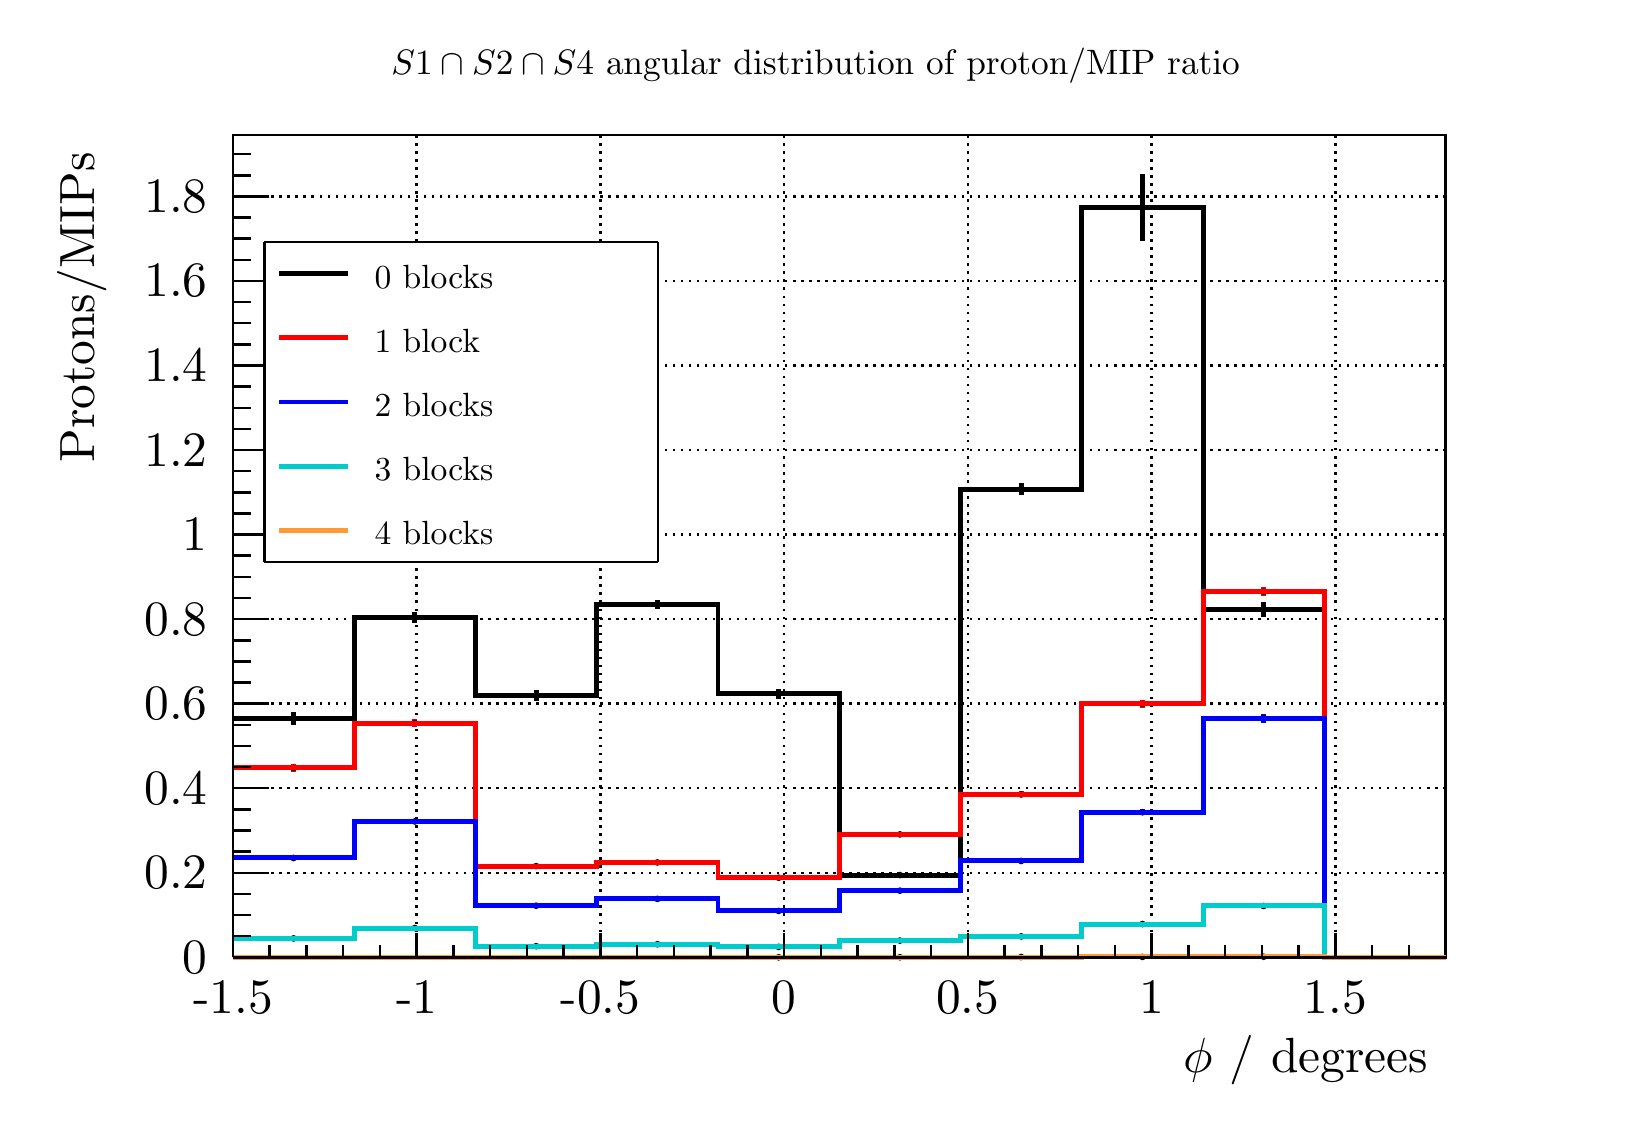
\begin{tikzpicture}
\pgfdeclareplotmark{cross} {
\pgfpathmoveto{\pgfpoint{-0.3\pgfplotmarksize}{\pgfplotmarksize}}
\pgfpathlineto{\pgfpoint{+0.3\pgfplotmarksize}{\pgfplotmarksize}}
\pgfpathlineto{\pgfpoint{+0.3\pgfplotmarksize}{0.3\pgfplotmarksize}}
\pgfpathlineto{\pgfpoint{+1\pgfplotmarksize}{0.3\pgfplotmarksize}}
\pgfpathlineto{\pgfpoint{+1\pgfplotmarksize}{-0.3\pgfplotmarksize}}
\pgfpathlineto{\pgfpoint{+0.3\pgfplotmarksize}{-0.3\pgfplotmarksize}}
\pgfpathlineto{\pgfpoint{+0.3\pgfplotmarksize}{-1.\pgfplotmarksize}}
\pgfpathlineto{\pgfpoint{-0.3\pgfplotmarksize}{-1.\pgfplotmarksize}}
\pgfpathlineto{\pgfpoint{-0.3\pgfplotmarksize}{-0.3\pgfplotmarksize}}
\pgfpathlineto{\pgfpoint{-1.\pgfplotmarksize}{-0.3\pgfplotmarksize}}
\pgfpathlineto{\pgfpoint{-1.\pgfplotmarksize}{0.3\pgfplotmarksize}}
\pgfpathlineto{\pgfpoint{-0.3\pgfplotmarksize}{0.3\pgfplotmarksize}}
\pgfpathclose
\pgfusepathqstroke
}
\pgfdeclareplotmark{cross*} {
\pgfpathmoveto{\pgfpoint{-0.3\pgfplotmarksize}{\pgfplotmarksize}}
\pgfpathlineto{\pgfpoint{+0.3\pgfplotmarksize}{\pgfplotmarksize}}
\pgfpathlineto{\pgfpoint{+0.3\pgfplotmarksize}{0.3\pgfplotmarksize}}
\pgfpathlineto{\pgfpoint{+1\pgfplotmarksize}{0.3\pgfplotmarksize}}
\pgfpathlineto{\pgfpoint{+1\pgfplotmarksize}{-0.3\pgfplotmarksize}}
\pgfpathlineto{\pgfpoint{+0.3\pgfplotmarksize}{-0.3\pgfplotmarksize}}
\pgfpathlineto{\pgfpoint{+0.3\pgfplotmarksize}{-1.\pgfplotmarksize}}
\pgfpathlineto{\pgfpoint{-0.3\pgfplotmarksize}{-1.\pgfplotmarksize}}
\pgfpathlineto{\pgfpoint{-0.3\pgfplotmarksize}{-0.3\pgfplotmarksize}}
\pgfpathlineto{\pgfpoint{-1.\pgfplotmarksize}{-0.3\pgfplotmarksize}}
\pgfpathlineto{\pgfpoint{-1.\pgfplotmarksize}{0.3\pgfplotmarksize}}
\pgfpathlineto{\pgfpoint{-0.3\pgfplotmarksize}{0.3\pgfplotmarksize}}
\pgfpathclose
\pgfusepathqfillstroke
}
\pgfdeclareplotmark{newstar} {
\pgfpathmoveto{\pgfqpoint{0pt}{\pgfplotmarksize}}
\pgfpathlineto{\pgfqpointpolar{44}{0.5\pgfplotmarksize}}
\pgfpathlineto{\pgfqpointpolar{18}{\pgfplotmarksize}}
\pgfpathlineto{\pgfqpointpolar{-20}{0.5\pgfplotmarksize}}
\pgfpathlineto{\pgfqpointpolar{-54}{\pgfplotmarksize}}
\pgfpathlineto{\pgfqpointpolar{-90}{0.5\pgfplotmarksize}}
\pgfpathlineto{\pgfqpointpolar{234}{\pgfplotmarksize}}
\pgfpathlineto{\pgfqpointpolar{198}{0.5\pgfplotmarksize}}
\pgfpathlineto{\pgfqpointpolar{162}{\pgfplotmarksize}}
\pgfpathlineto{\pgfqpointpolar{134}{0.5\pgfplotmarksize}}
\pgfpathclose
\pgfusepathqstroke
}
\pgfdeclareplotmark{newstar*} {
\pgfpathmoveto{\pgfqpoint{0pt}{\pgfplotmarksize}}
\pgfpathlineto{\pgfqpointpolar{44}{0.5\pgfplotmarksize}}
\pgfpathlineto{\pgfqpointpolar{18}{\pgfplotmarksize}}
\pgfpathlineto{\pgfqpointpolar{-20}{0.5\pgfplotmarksize}}
\pgfpathlineto{\pgfqpointpolar{-54}{\pgfplotmarksize}}
\pgfpathlineto{\pgfqpointpolar{-90}{0.5\pgfplotmarksize}}
\pgfpathlineto{\pgfqpointpolar{234}{\pgfplotmarksize}}
\pgfpathlineto{\pgfqpointpolar{198}{0.5\pgfplotmarksize}}
\pgfpathlineto{\pgfqpointpolar{162}{\pgfplotmarksize}}
\pgfpathlineto{\pgfqpointpolar{134}{0.5\pgfplotmarksize}}
\pgfpathclose
\pgfusepathqfillstroke
}
\definecolor{c}{rgb}{1,1,1};
\draw [color=c, fill=c] (0,0) rectangle (20,13.5632);
\draw [color=c, fill=c] (2.6,1.76322) rectangle (18,12.2069);
\definecolor{c}{rgb}{0,0,0};
\draw [c,line width=0.9] (2.6,1.76322) -- (2.6,12.2069) -- (18,12.2069) -- (18,1.76322) -- (2.6,1.76322);
\definecolor{c}{rgb}{1,1,1};
\draw [color=c, fill=c] (2.6,1.76322) rectangle (18,12.2069);
\definecolor{c}{rgb}{0,0,0};
\draw [c,line width=0.9] (2.6,1.76322) -- (2.6,12.2069) -- (18,12.2069) -- (18,1.76322) -- (2.6,1.76322);
\draw [c,line width=0.9] (2.6,1.76322) -- (18,1.76322);
\draw [c,dotted,line width=0.9] (2.6,12.2069) -- (2.6,1.76322);
\draw [c,dotted,line width=0.9] (4.93333,12.2069) -- (4.93333,1.76322);
\draw [c,dotted,line width=0.9] (7.26667,12.2069) -- (7.26667,1.76322);
\draw [c,dotted,line width=0.9] (9.6,12.2069) -- (9.6,1.76322);
\draw [c,dotted,line width=0.9] (11.9333,12.2069) -- (11.9333,1.76322);
\draw [c,dotted,line width=0.9] (14.2667,12.2069) -- (14.2667,1.76322);
\draw [c,dotted,line width=0.9] (16.6,12.2069) -- (16.6,1.76322);
\draw [c,dotted,line width=0.9] (16.6,12.2069) -- (16.6,1.76322);
\draw [c,line width=0.9] (2.6,1.76322) -- (2.6,12.2069);
\draw [c,dotted,line width=0.9] (18,1.76331) -- (2.6,1.76331);
\draw [c,dotted,line width=0.9] (18,2.83706) -- (2.6,2.83706);
\draw [c,dotted,line width=0.9] (18,3.91082) -- (2.6,3.91082);
\draw [c,dotted,line width=0.9] (18,4.98457) -- (2.6,4.98457);
\draw [c,dotted,line width=0.9] (18,6.05832) -- (2.6,6.05832);
\draw [c,dotted,line width=0.9] (18,7.13207) -- (2.6,7.13207);
\draw [c,dotted,line width=0.9] (18,8.20583) -- (2.6,8.20583);
\draw [c,dotted,line width=0.9] (18,9.27958) -- (2.6,9.27958);
\draw [c,dotted,line width=0.9] (18,10.3533) -- (2.6,10.3533);
\draw [c,dotted,line width=0.9] (18,11.4271) -- (2.6,11.4271);
\draw [c,dotted,line width=0.9] (18,1.76331) -- (2.6,1.76331);
\draw [c,dotted,line width=0.9] (18,11.4271) -- (2.6,11.4271);
\definecolor{c}{rgb}{0,0,0.6};
\draw [c,line width=0.9] (2.6,1.76331) -- (4.14,1.76331) -- (4.14,1.76331) -- (5.68,1.76331) -- (5.68,1.76331) -- (7.22,1.76331) -- (7.22,1.76331) -- (8.76,1.76331) -- (8.76,1.76331) -- (10.3,1.76331) -- (10.3,1.76331) -- (11.84,1.76331) --
 (11.84,1.76331) -- (13.38,1.76331) -- (13.38,1.76331) -- (14.92,1.76331) -- (14.92,1.76331) -- (16.46,1.76331) -- (16.46,1.76331) -- (18,1.76331);
\definecolor{c}{rgb}{0,0,0};
\draw [c,line width=0.9] (2.6,1.76322) -- (18,1.76322);
\draw [anchor= east] (18,0.461149) node[scale=1.78699, color=c, rotate=0]{$\phi$ / degrees};
\draw [c,line width=0.9] (2.6,2.07653) -- (2.6,1.76322);
\draw [c,line width=0.9] (3.06667,1.91987) -- (3.06667,1.76322);
\draw [c,line width=0.9] (3.53333,1.91987) -- (3.53333,1.76322);
\draw [c,line width=0.9] (4,1.91987) -- (4,1.76322);
\draw [c,line width=0.9] (4.46667,1.91987) -- (4.46667,1.76322);
\draw [c,line width=0.9] (4.93333,2.07653) -- (4.93333,1.76322);
\draw [c,line width=0.9] (5.4,1.91987) -- (5.4,1.76322);
\draw [c,line width=0.9] (5.86667,1.91987) -- (5.86667,1.76322);
\draw [c,line width=0.9] (6.33333,1.91987) -- (6.33333,1.76322);
\draw [c,line width=0.9] (6.8,1.91987) -- (6.8,1.76322);
\draw [c,line width=0.9] (7.26667,2.07653) -- (7.26667,1.76322);
\draw [c,line width=0.9] (7.73333,1.91987) -- (7.73333,1.76322);
\draw [c,line width=0.9] (8.2,1.91987) -- (8.2,1.76322);
\draw [c,line width=0.9] (8.66667,1.91987) -- (8.66667,1.76322);
\draw [c,line width=0.9] (9.13333,1.91987) -- (9.13333,1.76322);
\draw [c,line width=0.9] (9.6,2.07653) -- (9.6,1.76322);
\draw [c,line width=0.9] (10.0667,1.91987) -- (10.0667,1.76322);
\draw [c,line width=0.9] (10.5333,1.91987) -- (10.5333,1.76322);
\draw [c,line width=0.9] (11,1.91987) -- (11,1.76322);
\draw [c,line width=0.9] (11.4667,1.91987) -- (11.4667,1.76322);
\draw [c,line width=0.9] (11.9333,2.07653) -- (11.9333,1.76322);
\draw [c,line width=0.9] (12.4,1.91987) -- (12.4,1.76322);
\draw [c,line width=0.9] (12.8667,1.91987) -- (12.8667,1.76322);
\draw [c,line width=0.9] (13.3333,1.91987) -- (13.3333,1.76322);
\draw [c,line width=0.9] (13.8,1.91987) -- (13.8,1.76322);
\draw [c,line width=0.9] (14.2667,2.07653) -- (14.2667,1.76322);
\draw [c,line width=0.9] (14.7333,1.91987) -- (14.7333,1.76322);
\draw [c,line width=0.9] (15.2,1.91987) -- (15.2,1.76322);
\draw [c,line width=0.9] (15.6667,1.91987) -- (15.6667,1.76322);
\draw [c,line width=0.9] (16.1333,1.91987) -- (16.1333,1.76322);
\draw [c,line width=0.9] (16.6,2.07653) -- (16.6,1.76322);
\draw [c,line width=0.9] (16.6,2.07653) -- (16.6,1.76322);
\draw [c,line width=0.9] (17.0667,1.91987) -- (17.0667,1.76322);
\draw [c,line width=0.9] (17.5333,1.91987) -- (17.5333,1.76322);
\draw [anchor=base] (2.6,1.04437) node[scale=1.78699, color=c, rotate=0]{-1.5};
\draw [anchor=base] (4.93333,1.04437) node[scale=1.78699, color=c, rotate=0]{-1};
\draw [anchor=base] (7.26667,1.04437) node[scale=1.78699, color=c, rotate=0]{-0.5};
\draw [anchor=base] (9.6,1.04437) node[scale=1.78699, color=c, rotate=0]{0};
\draw [anchor=base] (11.9333,1.04437) node[scale=1.78699, color=c, rotate=0]{0.5};
\draw [anchor=base] (14.2667,1.04437) node[scale=1.78699, color=c, rotate=0]{1};
\draw [anchor=base] (16.6,1.04437) node[scale=1.78699, color=c, rotate=0]{1.5};
\draw [c,line width=0.9] (2.6,1.76322) -- (2.6,12.2069);
\draw [anchor= east] (0.68,12.2069) node[scale=1.78699, color=c, rotate=90]{ Protons/MIPs};
\draw [c,line width=0.9] (3.062,1.76331) -- (2.6,1.76331);
\draw [c,line width=0.9] (2.831,2.03175) -- (2.6,2.03175);
\draw [c,line width=0.9] (2.831,2.30019) -- (2.6,2.30019);
\draw [c,line width=0.9] (2.831,2.56863) -- (2.6,2.56863);
\draw [c,line width=0.9] (3.062,2.83706) -- (2.6,2.83706);
\draw [c,line width=0.9] (2.831,3.1055) -- (2.6,3.1055);
\draw [c,line width=0.9] (2.831,3.37394) -- (2.6,3.37394);
\draw [c,line width=0.9] (2.831,3.64238) -- (2.6,3.64238);
\draw [c,line width=0.9] (3.062,3.91082) -- (2.6,3.91082);
\draw [c,line width=0.9] (2.831,4.17925) -- (2.6,4.17925);
\draw [c,line width=0.9] (2.831,4.44769) -- (2.6,4.44769);
\draw [c,line width=0.9] (2.831,4.71613) -- (2.6,4.71613);
\draw [c,line width=0.9] (3.062,4.98457) -- (2.6,4.98457);
\draw [c,line width=0.9] (2.831,5.25301) -- (2.6,5.25301);
\draw [c,line width=0.9] (2.831,5.52145) -- (2.6,5.52145);
\draw [c,line width=0.9] (2.831,5.78988) -- (2.6,5.78988);
\draw [c,line width=0.9] (3.062,6.05832) -- (2.6,6.05832);
\draw [c,line width=0.9] (2.831,6.32676) -- (2.6,6.32676);
\draw [c,line width=0.9] (2.831,6.5952) -- (2.6,6.5952);
\draw [c,line width=0.9] (2.831,6.86364) -- (2.6,6.86364);
\draw [c,line width=0.9] (3.062,7.13207) -- (2.6,7.13207);
\draw [c,line width=0.9] (2.831,7.40051) -- (2.6,7.40051);
\draw [c,line width=0.9] (2.831,7.66895) -- (2.6,7.66895);
\draw [c,line width=0.9] (2.831,7.93739) -- (2.6,7.93739);
\draw [c,line width=0.9] (3.062,8.20583) -- (2.6,8.20583);
\draw [c,line width=0.9] (2.831,8.47427) -- (2.6,8.47427);
\draw [c,line width=0.9] (2.831,8.7427) -- (2.6,8.7427);
\draw [c,line width=0.9] (2.831,9.01114) -- (2.6,9.01114);
\draw [c,line width=0.9] (3.062,9.27958) -- (2.6,9.27958);
\draw [c,line width=0.9] (2.831,9.54802) -- (2.6,9.54802);
\draw [c,line width=0.9] (2.831,9.81646) -- (2.6,9.81646);
\draw [c,line width=0.9] (2.831,10.0849) -- (2.6,10.0849);
\draw [c,line width=0.9] (3.062,10.3533) -- (2.6,10.3533);
\draw [c,line width=0.9] (2.831,10.6218) -- (2.6,10.6218);
\draw [c,line width=0.9] (2.831,10.8902) -- (2.6,10.8902);
\draw [c,line width=0.9] (2.831,11.1586) -- (2.6,11.1586);
\draw [c,line width=0.9] (3.062,11.4271) -- (2.6,11.4271);
\draw [c,line width=0.9] (3.062,1.76331) -- (2.6,1.76331);
\draw [c,line width=0.9] (3.062,11.4271) -- (2.6,11.4271);
\draw [c,line width=0.9] (2.831,11.6955) -- (2.6,11.6955);
\draw [c,line width=0.9] (2.831,11.964) -- (2.6,11.964);
\draw [anchor= east] (2.5,1.76331) node[scale=1.78699, color=c, rotate=0]{0};
\draw [anchor= east] (2.5,2.83706) node[scale=1.78699, color=c, rotate=0]{0.2};
\draw [anchor= east] (2.5,3.91082) node[scale=1.78699, color=c, rotate=0]{0.4};
\draw [anchor= east] (2.5,4.98457) node[scale=1.78699, color=c, rotate=0]{0.6};
\draw [anchor= east] (2.5,6.05832) node[scale=1.78699, color=c, rotate=0]{0.8};
\draw [anchor= east] (2.5,7.13207) node[scale=1.78699, color=c, rotate=0]{1};
\draw [anchor= east] (2.5,8.20583) node[scale=1.78699, color=c, rotate=0]{1.2};
\draw [anchor= east] (2.5,9.27958) node[scale=1.78699, color=c, rotate=0]{1.4};
\draw [anchor= east] (2.5,10.3533) node[scale=1.78699, color=c, rotate=0]{1.6};
\draw [anchor= east] (2.5,11.4271) node[scale=1.78699, color=c, rotate=0]{1.8};
\draw [c,line width=1.8] (3.37,4.71121) -- (3.37,4.79669);
\draw [c,line width=1.8] (3.37,4.79669) -- (3.37,4.88216);
\foreach \P in {(3.37,4.79669)}{\draw[mark options={color=c,fill=c},mark size=2.402402pt,mark=*,mark size=1pt] plot coordinates {\P};}
\draw [c,line width=1.8] (4.91,6.01196) -- (4.91,6.07817);
\draw [c,line width=1.8] (4.91,6.07817) -- (4.91,6.14439);
\foreach \P in {(4.91,6.07817)}{\draw[mark options={color=c,fill=c},mark size=2.402402pt,mark=*,mark size=1pt] plot coordinates {\P};}
\draw [c,line width=1.8] (6.45,5.02248) -- (6.45,5.09174);
\draw [c,line width=1.8] (6.45,5.09174) -- (6.45,5.16101);
\foreach \P in {(6.45,5.09174)}{\draw[mark options={color=c,fill=c},mark size=2.402402pt,mark=*,mark size=1pt] plot coordinates {\P};}
\draw [c,line width=1.8] (7.99,6.19214) -- (7.99,6.24525);
\draw [c,line width=1.8] (7.99,6.24525) -- (7.99,6.29836);
\foreach \P in {(7.99,6.24525)}{\draw[mark options={color=c,fill=c},mark size=2.402402pt,mark=*,mark size=1pt] plot coordinates {\P};}
\draw [c,line width=1.8] (9.53,5.04647) -- (9.53,5.11033);
\draw [c,line width=1.8] (9.53,5.11033) -- (9.53,5.1742);
\foreach \P in {(9.53,5.11033)}{\draw[mark options={color=c,fill=c},mark size=2.402402pt,mark=*,mark size=1pt] plot coordinates {\P};}
\draw [c,line width=1.8] (11.07,2.77883) -- (11.07,2.80789);
\draw [c,line width=1.8] (11.07,2.80789) -- (11.07,2.83695);
\foreach \P in {(11.07,2.80789)}{\draw[mark options={color=c,fill=c},mark size=2.402402pt,mark=*,mark size=1pt] plot coordinates {\P};}
\draw [c,line width=1.8] (12.61,7.6402) -- (12.61,7.71067);
\draw [c,line width=1.8] (12.61,7.71067) -- (12.61,7.78113);
\foreach \P in {(12.61,7.71067)}{\draw[mark options={color=c,fill=c},mark size=2.402402pt,mark=*,mark size=1pt] plot coordinates {\P};}
\draw [c,line width=1.8] (14.15,10.8621) -- (14.15,11.2859);
\draw [c,line width=1.8] (14.15,11.2859) -- (14.15,11.7096);
\foreach \P in {(14.15,11.2859)}{\draw[mark options={color=c,fill=c},mark size=2.402402pt,mark=*,mark size=1pt] plot coordinates {\P};}
\draw [c,line width=1.8] (15.69,6.08849) -- (15.69,6.18452);
\draw [c,line width=1.8] (15.69,6.18452) -- (15.69,6.28056);
\foreach \P in {(15.69,6.18452)}{\draw[mark options={color=c,fill=c},mark size=2.402402pt,mark=*,mark size=1pt] plot coordinates {\P};}
\draw [c,line width=1.8] (2.6,4.79669) -- (4.14,4.79669) -- (4.14,6.07817) -- (5.68,6.07817) -- (5.68,5.09174) -- (7.22,5.09174) -- (7.22,6.24525) -- (8.76,6.24525) -- (8.76,5.11033) -- (10.3,5.11033) -- (10.3,2.80789) -- (11.84,2.80789) --
 (11.84,7.71067) -- (13.38,7.71067) -- (13.38,11.2859) -- (14.92,11.2859) -- (14.92,6.18452) -- (16.46,6.18452) -- (16.46,1.76322) -- (18,1.76322);
\definecolor{c}{rgb}{1,0,0};
\draw [c,line width=1.8] (3.37,4.11953) -- (3.37,4.1684);
\draw [c,line width=1.8] (3.37,4.1684) -- (3.37,4.21728);
\definecolor{c}{rgb}{0,0,0};
\foreach \P in {(3.37,4.1684)}{\draw[mark options={color=c,fill=c},mark size=2.402402pt,mark=*,mark size=1pt] plot coordinates {\P};}
\definecolor{c}{rgb}{1,0,0};
\draw [c,line width=1.8] (4.91,4.69275) -- (4.91,4.73893);
\draw [c,line width=1.8] (4.91,4.73893) -- (4.91,4.78512);
\definecolor{c}{rgb}{0,0,0};
\foreach \P in {(4.91,4.73893)}{\draw[mark options={color=c,fill=c},mark size=2.402402pt,mark=*,mark size=1pt] plot coordinates {\P};}
\definecolor{c}{rgb}{1,0,0};
\draw [c,line width=1.8] (6.45,2.89934) -- (6.45,2.92218);
\draw [c,line width=1.8] (6.45,2.92218) -- (6.45,2.94503);
\definecolor{c}{rgb}{0,0,0};
\foreach \P in {(6.45,2.92218)}{\draw[mark options={color=c,fill=c},mark size=2.402402pt,mark=*,mark size=1pt] plot coordinates {\P};}
\definecolor{c}{rgb}{1,0,0};
\draw [c,line width=1.8] (7.99,2.94718) -- (7.99,2.96885);
\draw [c,line width=1.8] (7.99,2.96885) -- (7.99,2.99052);
\definecolor{c}{rgb}{0,0,0};
\foreach \P in {(7.99,2.96885)}{\draw[mark options={color=c,fill=c},mark size=2.402402pt,mark=*,mark size=1pt] plot coordinates {\P};}
\definecolor{c}{rgb}{1,0,0};
\draw [c,line width=1.8] (9.53,2.75545) -- (9.53,2.77466);
\draw [c,line width=1.8] (9.53,2.77466) -- (9.53,2.79386);
\definecolor{c}{rgb}{0,0,0};
\foreach \P in {(9.53,2.77466)}{\draw[mark options={color=c,fill=c},mark size=2.402402pt,mark=*,mark size=1pt] plot coordinates {\P};}
\definecolor{c}{rgb}{1,0,0};
\draw [c,line width=1.8] (11.07,3.29785) -- (11.07,3.32473);
\draw [c,line width=1.8] (11.07,3.32473) -- (11.07,3.35162);
\definecolor{c}{rgb}{0,0,0};
\foreach \P in {(11.07,3.32473)}{\draw[mark options={color=c,fill=c},mark size=2.402402pt,mark=*,mark size=1pt] plot coordinates {\P};}
\definecolor{c}{rgb}{1,0,0};
\draw [c,line width=1.8] (12.61,3.79369) -- (12.61,3.83174);
\draw [c,line width=1.8] (12.61,3.83174) -- (12.61,3.86979);
\definecolor{c}{rgb}{0,0,0};
\foreach \P in {(12.61,3.83174)}{\draw[mark options={color=c,fill=c},mark size=2.402402pt,mark=*,mark size=1pt] plot coordinates {\P};}
\definecolor{c}{rgb}{1,0,0};
\draw [c,line width=1.8] (14.15,4.92996) -- (14.15,4.9825);
\draw [c,line width=1.8] (14.15,4.9825) -- (14.15,5.03505);
\definecolor{c}{rgb}{0,0,0};
\foreach \P in {(14.15,4.9825)}{\draw[mark options={color=c,fill=c},mark size=2.402402pt,mark=*,mark size=1pt] plot coordinates {\P};}
\definecolor{c}{rgb}{1,0,0};
\draw [c,line width=1.8] (15.69,6.35124) -- (15.69,6.40788);
\draw [c,line width=1.8] (15.69,6.40788) -- (15.69,6.46452);
\definecolor{c}{rgb}{0,0,0};
\foreach \P in {(15.69,6.40788)}{\draw[mark options={color=c,fill=c},mark size=2.402402pt,mark=*,mark size=1pt] plot coordinates {\P};}
\definecolor{c}{rgb}{1,0,0};
\draw [c,line width=1.8] (2.6,4.1684) -- (4.14,4.1684) -- (4.14,4.73893) -- (5.68,4.73893) -- (5.68,2.92218) -- (7.22,2.92218) -- (7.22,2.96885) -- (8.76,2.96885) -- (8.76,2.77466) -- (10.3,2.77466) -- (10.3,3.32473) -- (11.84,3.32473) --
 (11.84,3.83174) -- (13.38,3.83174) -- (13.38,4.9825) -- (14.92,4.9825) -- (14.92,6.40788) -- (16.46,6.40788) -- (16.46,1.76322) -- (18,1.76322);
\definecolor{c}{rgb}{0,0,1};
\draw [c,line width=1.8] (3.37,2.99342) -- (3.37,3.0254);
\draw [c,line width=1.8] (3.37,3.0254) -- (3.37,3.05738);
\definecolor{c}{rgb}{0,0,0};
\foreach \P in {(3.37,3.0254)}{\draw[mark options={color=c,fill=c},mark size=2.402402pt,mark=*,mark size=1pt] plot coordinates {\P};}
\definecolor{c}{rgb}{0,0,1};
\draw [c,line width=1.8] (4.91,3.45569) -- (4.91,3.48922);
\draw [c,line width=1.8] (4.91,3.48922) -- (4.91,3.52275);
\definecolor{c}{rgb}{0,0,0};
\foreach \P in {(4.91,3.48922)}{\draw[mark options={color=c,fill=c},mark size=2.402402pt,mark=*,mark size=1pt] plot coordinates {\P};}
\definecolor{c}{rgb}{0,0,1};
\draw [c,line width=1.8] (6.45,2.40459) -- (6.45,2.4189);
\draw [c,line width=1.8] (6.45,2.4189) -- (6.45,2.4332);
\definecolor{c}{rgb}{0,0,0};
\foreach \P in {(6.45,2.4189)}{\draw[mark options={color=c,fill=c},mark size=2.402402pt,mark=*,mark size=1pt] plot coordinates {\P};}
\definecolor{c}{rgb}{0,0,1};
\draw [c,line width=1.8] (7.99,2.49152) -- (7.99,2.50575);
\draw [c,line width=1.8] (7.99,2.50575) -- (7.99,2.51998);
\definecolor{c}{rgb}{0,0,0};
\foreach \P in {(7.99,2.50575)}{\draw[mark options={color=c,fill=c},mark size=2.402402pt,mark=*,mark size=1pt] plot coordinates {\P};}
\definecolor{c}{rgb}{0,0,1};
\draw [c,line width=1.8] (9.53,2.34143) -- (9.53,2.35363);
\draw [c,line width=1.8] (9.53,2.35363) -- (9.53,2.36583);
\definecolor{c}{rgb}{0,0,0};
\foreach \P in {(9.53,2.35363)}{\draw[mark options={color=c,fill=c},mark size=2.402402pt,mark=*,mark size=1pt] plot coordinates {\P};}
\definecolor{c}{rgb}{0,0,1};
\draw [c,line width=1.8] (11.07,2.59294) -- (11.07,2.61003);
\draw [c,line width=1.8] (11.07,2.61003) -- (11.07,2.62713);
\definecolor{c}{rgb}{0,0,0};
\foreach \P in {(11.07,2.61003)}{\draw[mark options={color=c,fill=c},mark size=2.402402pt,mark=*,mark size=1pt] plot coordinates {\P};}
\definecolor{c}{rgb}{0,0,1};
\draw [c,line width=1.8] (12.61,2.96164) -- (12.61,2.98755);
\draw [c,line width=1.8] (12.61,2.98755) -- (12.61,3.01347);
\definecolor{c}{rgb}{0,0,0};
\foreach \P in {(12.61,2.98755)}{\draw[mark options={color=c,fill=c},mark size=2.402402pt,mark=*,mark size=1pt] plot coordinates {\P};}
\definecolor{c}{rgb}{0,0,1};
\draw [c,line width=1.8] (14.15,3.56827) -- (14.15,3.60626);
\draw [c,line width=1.8] (14.15,3.60626) -- (14.15,3.64424);
\definecolor{c}{rgb}{0,0,0};
\foreach \P in {(14.15,3.60626)}{\draw[mark options={color=c,fill=c},mark size=2.402402pt,mark=*,mark size=1pt] plot coordinates {\P};}
\definecolor{c}{rgb}{0,0,1};
\draw [c,line width=1.8] (15.69,4.74022) -- (15.69,4.79919);
\draw [c,line width=1.8] (15.69,4.79919) -- (15.69,4.85817);
\definecolor{c}{rgb}{0,0,0};
\foreach \P in {(15.69,4.79919)}{\draw[mark options={color=c,fill=c},mark size=2.402402pt,mark=*,mark size=1pt] plot coordinates {\P};}
\definecolor{c}{rgb}{0,0,1};
\draw [c,line width=1.8] (2.6,3.0254) -- (4.14,3.0254) -- (4.14,3.48922) -- (5.68,3.48922) -- (5.68,2.4189) -- (7.22,2.4189) -- (7.22,2.50575) -- (8.76,2.50575) -- (8.76,2.35363) -- (10.3,2.35363) -- (10.3,2.61003) -- (11.84,2.61003) --
 (11.84,2.98755) -- (13.38,2.98755) -- (13.38,3.60626) -- (14.92,3.60626) -- (14.92,4.79919) -- (16.46,4.79919) -- (16.46,1.76322) -- (18,1.76322);
\definecolor{c}{rgb}{0,0.8,0.8};
\draw [c,line width=1.8] (3.37,1.98645) -- (3.37,2.00382);
\draw [c,line width=1.8] (3.37,2.00382) -- (3.37,2.02119);
\definecolor{c}{rgb}{0,0,0};
\foreach \P in {(3.37,2.00382)}{\draw[mark options={color=c,fill=c},mark size=2.402402pt,mark=*,mark size=1pt] plot coordinates {\P};}
\definecolor{c}{rgb}{0,0.8,0.8};
\draw [c,line width=1.8] (4.91,2.1156) -- (4.91,2.1351);
\draw [c,line width=1.8] (4.91,2.1351) -- (4.91,2.1546);
\definecolor{c}{rgb}{0,0,0};
\foreach \P in {(4.91,2.1351)}{\draw[mark options={color=c,fill=c},mark size=2.402402pt,mark=*,mark size=1pt] plot coordinates {\P};}
\definecolor{c}{rgb}{0,0.8,0.8};
\draw [c,line width=1.8] (6.45,1.89731) -- (6.45,1.90524);
\draw [c,line width=1.8] (6.45,1.90524) -- (6.45,1.91317);
\definecolor{c}{rgb}{0,0,0};
\foreach \P in {(6.45,1.90524)}{\draw[mark options={color=c,fill=c},mark size=2.402402pt,mark=*,mark size=1pt] plot coordinates {\P};}
\definecolor{c}{rgb}{0,0.8,0.8};
\draw [c,line width=1.8] (7.99,1.92127) -- (7.99,1.92926);
\draw [c,line width=1.8] (7.99,1.92926) -- (7.99,1.93725);
\definecolor{c}{rgb}{0,0,0};
\foreach \P in {(7.99,1.92926)}{\draw[mark options={color=c,fill=c},mark size=2.402402pt,mark=*,mark size=1pt] plot coordinates {\P};}
\definecolor{c}{rgb}{0,0.8,0.8};
\draw [c,line width=1.8] (9.53,1.88965) -- (9.53,1.89653);
\draw [c,line width=1.8] (9.53,1.89653) -- (9.53,1.90341);
\definecolor{c}{rgb}{0,0,0};
\foreach \P in {(9.53,1.89653)}{\draw[mark options={color=c,fill=c},mark size=2.402402pt,mark=*,mark size=1pt] plot coordinates {\P};}
\definecolor{c}{rgb}{0,0.8,0.8};
\draw [c,line width=1.8] (11.07,1.96599) -- (11.07,1.97605);
\draw [c,line width=1.8] (11.07,1.97605) -- (11.07,1.98611);
\definecolor{c}{rgb}{0,0,0};
\foreach \P in {(11.07,1.97605)}{\draw[mark options={color=c,fill=c},mark size=2.402402pt,mark=*,mark size=1pt] plot coordinates {\P};}
\definecolor{c}{rgb}{0,0.8,0.8};
\draw [c,line width=1.8] (12.61,2.01471) -- (12.61,2.0295);
\draw [c,line width=1.8] (12.61,2.0295) -- (12.61,2.04429);
\definecolor{c}{rgb}{0,0,0};
\foreach \P in {(12.61,2.0295)}{\draw[mark options={color=c,fill=c},mark size=2.402402pt,mark=*,mark size=1pt] plot coordinates {\P};}
\definecolor{c}{rgb}{0,0.8,0.8};
\draw [c,line width=1.8] (14.15,2.16322) -- (14.15,2.18639);
\draw [c,line width=1.8] (14.15,2.18639) -- (14.15,2.20956);
\definecolor{c}{rgb}{0,0,0};
\foreach \P in {(14.15,2.18639)}{\draw[mark options={color=c,fill=c},mark size=2.402402pt,mark=*,mark size=1pt] plot coordinates {\P};}
\definecolor{c}{rgb}{0,0.8,0.8};
\draw [c,line width=1.8] (15.69,2.37467) -- (15.69,2.41691);
\draw [c,line width=1.8] (15.69,2.41691) -- (15.69,2.45915);
\definecolor{c}{rgb}{0,0,0};
\foreach \P in {(15.69,2.41691)}{\draw[mark options={color=c,fill=c},mark size=2.402402pt,mark=*,mark size=1pt] plot coordinates {\P};}
\definecolor{c}{rgb}{0,0.8,0.8};
\draw [c,line width=1.8] (2.6,2.00382) -- (4.14,2.00382) -- (4.14,2.1351) -- (5.68,2.1351) -- (5.68,1.90524) -- (7.22,1.90524) -- (7.22,1.92926) -- (8.76,1.92926) -- (8.76,1.89653) -- (10.3,1.89653) -- (10.3,1.97605) -- (11.84,1.97605) --
 (11.84,2.0295) -- (13.38,2.0295) -- (13.38,2.18639) -- (14.92,2.18639) -- (14.92,2.41691) -- (16.46,2.41691) -- (16.46,1.76322) -- (18,1.76322);
\definecolor{c}{rgb}{1,0.6,0.2};
\draw [c,line width=1.8] (9.53,1.76322) -- (9.53,1.76399);
\draw [c,line width=1.8] (9.53,1.76399) -- (9.53,1.76476);
\definecolor{c}{rgb}{0,0,0};
\foreach \P in {(9.53,1.76399)}{\draw[mark options={color=c,fill=c},mark size=2.402402pt,mark=*,mark size=1pt] plot coordinates {\P};}
\definecolor{c}{rgb}{1,0.6,0.2};
\draw [c,line width=1.8] (11.07,1.76366) -- (11.07,1.76464);
\draw [c,line width=1.8] (11.07,1.76464) -- (11.07,1.76562);
\definecolor{c}{rgb}{0,0,0};
\foreach \P in {(11.07,1.76464)}{\draw[mark options={color=c,fill=c},mark size=2.402402pt,mark=*,mark size=1pt] plot coordinates {\P};}
\definecolor{c}{rgb}{1,0.6,0.2};
\draw [c,line width=1.8] (12.61,1.76559) -- (12.61,1.76699);
\draw [c,line width=1.8] (12.61,1.76699) -- (12.61,1.7684);
\definecolor{c}{rgb}{0,0,0};
\foreach \P in {(12.61,1.76699)}{\draw[mark options={color=c,fill=c},mark size=2.402402pt,mark=*,mark size=1pt] plot coordinates {\P};}
\definecolor{c}{rgb}{1,0.6,0.2};
\draw [c,line width=1.8] (14.15,1.76701) -- (14.15,1.76884);
\draw [c,line width=1.8] (14.15,1.76884) -- (14.15,1.77066);
\definecolor{c}{rgb}{0,0,0};
\foreach \P in {(14.15,1.76884)}{\draw[mark options={color=c,fill=c},mark size=2.402402pt,mark=*,mark size=1pt] plot coordinates {\P};}
\definecolor{c}{rgb}{1,0.6,0.2};
\draw [c,line width=1.8] (15.69,1.7683) -- (15.69,1.77128);
\draw [c,line width=1.8] (15.69,1.77128) -- (15.69,1.77426);
\definecolor{c}{rgb}{0,0,0};
\foreach \P in {(15.69,1.77128)}{\draw[mark options={color=c,fill=c},mark size=2.402402pt,mark=*,mark size=1pt] plot coordinates {\P};}
\definecolor{c}{rgb}{1,0.6,0.2};
\draw [c,line width=1.8] (2.6,1.76322) -- (4.14,1.76322) -- (4.14,1.76322) -- (5.68,1.76322) -- (5.68,1.76322) -- (7.22,1.76322) -- (7.22,1.76322) -- (8.76,1.76322) -- (8.76,1.76322) -- (10.3,1.76322) -- (10.3,1.76464) -- (11.84,1.76464) --
 (11.84,1.76699) -- (13.38,1.76699) -- (13.38,1.76884) -- (14.92,1.76884) -- (14.92,1.77128) -- (16.46,1.77128) -- (16.46,1.76322) -- (18,1.76322);
\definecolor{c}{rgb}{0,0,0};
\draw [c,line width=0.9] (2.6,1.76322) -- (18,1.76322);
\draw [c,line width=0.9] (2.6,2.07653) -- (2.6,1.76322);
\draw [c,line width=0.9] (3.06667,1.91987) -- (3.06667,1.76322);
\draw [c,line width=0.9] (3.53333,1.91987) -- (3.53333,1.76322);
\draw [c,line width=0.9] (4,1.91987) -- (4,1.76322);
\draw [c,line width=0.9] (4.46667,1.91987) -- (4.46667,1.76322);
\draw [c,line width=0.9] (4.93333,2.07653) -- (4.93333,1.76322);
\draw [c,line width=0.9] (5.4,1.91987) -- (5.4,1.76322);
\draw [c,line width=0.9] (5.86667,1.91987) -- (5.86667,1.76322);
\draw [c,line width=0.9] (6.33333,1.91987) -- (6.33333,1.76322);
\draw [c,line width=0.9] (6.8,1.91987) -- (6.8,1.76322);
\draw [c,line width=0.9] (7.26667,2.07653) -- (7.26667,1.76322);
\draw [c,line width=0.9] (7.73333,1.91987) -- (7.73333,1.76322);
\draw [c,line width=0.9] (8.2,1.91987) -- (8.2,1.76322);
\draw [c,line width=0.9] (8.66667,1.91987) -- (8.66667,1.76322);
\draw [c,line width=0.9] (9.13333,1.91987) -- (9.13333,1.76322);
\draw [c,line width=0.9] (9.6,2.07653) -- (9.6,1.76322);
\draw [c,line width=0.9] (10.0667,1.91987) -- (10.0667,1.76322);
\draw [c,line width=0.9] (10.5333,1.91987) -- (10.5333,1.76322);
\draw [c,line width=0.9] (11,1.91987) -- (11,1.76322);
\draw [c,line width=0.9] (11.4667,1.91987) -- (11.4667,1.76322);
\draw [c,line width=0.9] (11.9333,2.07653) -- (11.9333,1.76322);
\draw [c,line width=0.9] (12.4,1.91987) -- (12.4,1.76322);
\draw [c,line width=0.9] (12.8667,1.91987) -- (12.8667,1.76322);
\draw [c,line width=0.9] (13.3333,1.91987) -- (13.3333,1.76322);
\draw [c,line width=0.9] (13.8,1.91987) -- (13.8,1.76322);
\draw [c,line width=0.9] (14.2667,2.07653) -- (14.2667,1.76322);
\draw [c,line width=0.9] (14.7333,1.91987) -- (14.7333,1.76322);
\draw [c,line width=0.9] (15.2,1.91987) -- (15.2,1.76322);
\draw [c,line width=0.9] (15.6667,1.91987) -- (15.6667,1.76322);
\draw [c,line width=0.9] (16.1333,1.91987) -- (16.1333,1.76322);
\draw [c,line width=0.9] (16.6,2.07653) -- (16.6,1.76322);
\draw [c,line width=0.9] (16.6,2.07653) -- (16.6,1.76322);
\draw [c,line width=0.9] (17.0667,1.91987) -- (17.0667,1.76322);
\draw [c,line width=0.9] (17.5333,1.91987) -- (17.5333,1.76322);
\draw [c,line width=0.9] (2.6,1.76322) -- (2.6,12.2069);
\draw [c,line width=0.9] (3.062,1.76331) -- (2.6,1.76331);
\draw [c,line width=0.9] (2.831,2.03175) -- (2.6,2.03175);
\draw [c,line width=0.9] (2.831,2.30019) -- (2.6,2.30019);
\draw [c,line width=0.9] (2.831,2.56863) -- (2.6,2.56863);
\draw [c,line width=0.9] (3.062,2.83706) -- (2.6,2.83706);
\draw [c,line width=0.9] (2.831,3.1055) -- (2.6,3.1055);
\draw [c,line width=0.9] (2.831,3.37394) -- (2.6,3.37394);
\draw [c,line width=0.9] (2.831,3.64238) -- (2.6,3.64238);
\draw [c,line width=0.9] (3.062,3.91082) -- (2.6,3.91082);
\draw [c,line width=0.9] (2.831,4.17925) -- (2.6,4.17925);
\draw [c,line width=0.9] (2.831,4.44769) -- (2.6,4.44769);
\draw [c,line width=0.9] (2.831,4.71613) -- (2.6,4.71613);
\draw [c,line width=0.9] (3.062,4.98457) -- (2.6,4.98457);
\draw [c,line width=0.9] (2.831,5.25301) -- (2.6,5.25301);
\draw [c,line width=0.9] (2.831,5.52145) -- (2.6,5.52145);
\draw [c,line width=0.9] (2.831,5.78988) -- (2.6,5.78988);
\draw [c,line width=0.9] (3.062,6.05832) -- (2.6,6.05832);
\draw [c,line width=0.9] (2.831,6.32676) -- (2.6,6.32676);
\draw [c,line width=0.9] (2.831,6.5952) -- (2.6,6.5952);
\draw [c,line width=0.9] (2.831,6.86364) -- (2.6,6.86364);
\draw [c,line width=0.9] (3.062,7.13207) -- (2.6,7.13207);
\draw [c,line width=0.9] (2.831,7.40051) -- (2.6,7.40051);
\draw [c,line width=0.9] (2.831,7.66895) -- (2.6,7.66895);
\draw [c,line width=0.9] (2.831,7.93739) -- (2.6,7.93739);
\draw [c,line width=0.9] (3.062,8.20583) -- (2.6,8.20583);
\draw [c,line width=0.9] (2.831,8.47427) -- (2.6,8.47427);
\draw [c,line width=0.9] (2.831,8.7427) -- (2.6,8.7427);
\draw [c,line width=0.9] (2.831,9.01114) -- (2.6,9.01114);
\draw [c,line width=0.9] (3.062,9.27958) -- (2.6,9.27958);
\draw [c,line width=0.9] (2.831,9.54802) -- (2.6,9.54802);
\draw [c,line width=0.9] (2.831,9.81646) -- (2.6,9.81646);
\draw [c,line width=0.9] (2.831,10.0849) -- (2.6,10.0849);
\draw [c,line width=0.9] (3.062,10.3533) -- (2.6,10.3533);
\draw [c,line width=0.9] (2.831,10.6218) -- (2.6,10.6218);
\draw [c,line width=0.9] (2.831,10.8902) -- (2.6,10.8902);
\draw [c,line width=0.9] (2.831,11.1586) -- (2.6,11.1586);
\draw [c,line width=0.9] (3.062,11.4271) -- (2.6,11.4271);
\draw [c,line width=0.9] (3.062,1.76331) -- (2.6,1.76331);
\draw [c,line width=0.9] (3.062,11.4271) -- (2.6,11.4271);
\draw [c,line width=0.9] (2.831,11.6955) -- (2.6,11.6955);
\draw [c,line width=0.9] (2.831,11.964) -- (2.6,11.964);
\draw (10,13.0816) node[scale=1.27642, color=c, rotate=0]{$S1 \cap S2 \cap S4$ angular distribution of proton/MIP ratio};
\definecolor{c}{rgb}{1,1,1};
\draw [color=c, fill=c] (3,6.78161) rectangle (8,10.8506);
\definecolor{c}{rgb}{0,0,0};
\draw [c,line width=0.9] (3,6.78161) -- (8,6.78161);
\draw [c,line width=0.9] (8,6.78161) -- (8,10.8506);
\draw [c,line width=0.9] (8,10.8506) -- (3,10.8506);
\draw [c,line width=0.9] (3,10.8506) -- (3,6.78161);
\draw [anchor=base west] (4.25,10.2606) node[scale=1.2126, color=c, rotate=0]{0 blocks};
\draw [c,line width=1.8] (3.1875,10.4437) -- (4.0625,10.4437);
\draw [anchor=base west] (4.25,9.44678) node[scale=1.2126, color=c, rotate=0]{1 block};
\definecolor{c}{rgb}{1,0,0};
\draw [c,line width=1.8] (3.1875,9.62988) -- (4.0625,9.62988);
\definecolor{c}{rgb}{0,0,0};
\draw [anchor=base west] (4.25,8.63299) node[scale=1.2126, color=c, rotate=0]{2 blocks};
\definecolor{c}{rgb}{0,0,1};
\draw [c,line width=1.8] (3.1875,8.81609) -- (4.0625,8.81609);
\definecolor{c}{rgb}{0,0,0};
\draw [anchor=base west] (4.25,7.8192) node[scale=1.2126, color=c, rotate=0]{3 blocks};
\definecolor{c}{rgb}{0,0.8,0.8};
\draw [c,line width=1.8] (3.1875,8.0023) -- (4.0625,8.0023);
\definecolor{c}{rgb}{0,0,0};
\draw [anchor=base west] (4.25,7.0054) node[scale=1.2126, color=c, rotate=0]{4 blocks};
\definecolor{c}{rgb}{1,0.6,0.2};
\draw [c,line width=1.8] (3.1875,7.18851) -- (4.0625,7.18851);
\end{tikzpicture}

	    	\end{adjustbox}
    		\caption{Proton/MIP ratio in $S4$ for varying numbers of moderator blocks as a function of vertical off-axis angle, as measured from $S1$}
    		\label{fig:propiratio_s4_vert}
    	\end{minipage}	
   	\end{figure}
   
	\subsection{Flux normalization between detectors}
	
	Normalization factors for comparing the flux are calculated and shown in table~\ref{tab:fluxFactors}.
	These factors are calculated relative to the flux passing through $S3$ which covered the greatest angular extent of any of the timing points. 
	The angular positions of the various timing points are shown in figure~\ref{fig:beamAng}.
	
	\begin{figure}[h]
		
	\end{figure}
		
	The total flux passing through $S1$ and $S3$ is shown in figure~\ref{fig:s1s3all}.
	This flux is normalised such that its area is equal to 1.
	The factors are calculated by integrating this distribution between the angular limits of the other timing points.
	Table~\ref{tab:fluxFactors} shows the calculated factors for various timing points and overlaps.
	
	\begin{figure}[h]
		\begin{minipage}{0.49\textwidth}
			%\begin{adjustbox}{max totalsize={0.6\textwidth}{.5\textheight}}
			%	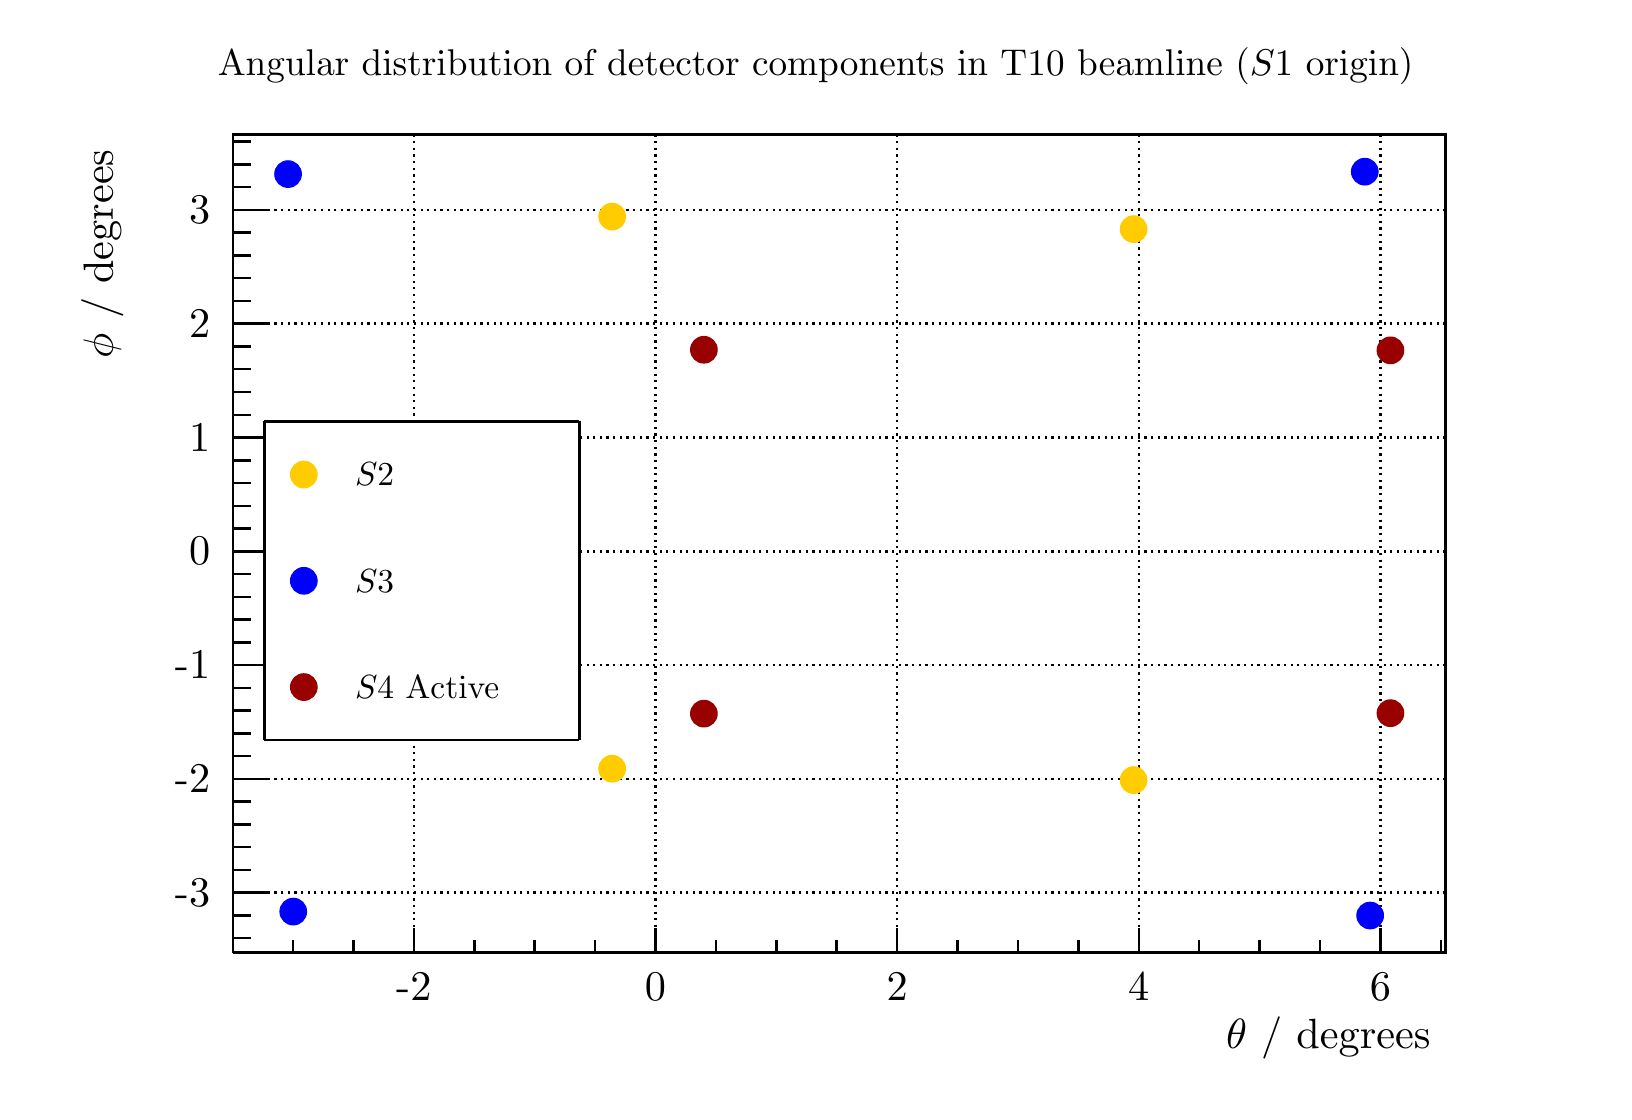
\begin{tikzpicture}
\pgfdeclareplotmark{cross} {
\pgfpathmoveto{\pgfpoint{-0.3\pgfplotmarksize}{\pgfplotmarksize}}
\pgfpathlineto{\pgfpoint{+0.3\pgfplotmarksize}{\pgfplotmarksize}}
\pgfpathlineto{\pgfpoint{+0.3\pgfplotmarksize}{0.3\pgfplotmarksize}}
\pgfpathlineto{\pgfpoint{+1\pgfplotmarksize}{0.3\pgfplotmarksize}}
\pgfpathlineto{\pgfpoint{+1\pgfplotmarksize}{-0.3\pgfplotmarksize}}
\pgfpathlineto{\pgfpoint{+0.3\pgfplotmarksize}{-0.3\pgfplotmarksize}}
\pgfpathlineto{\pgfpoint{+0.3\pgfplotmarksize}{-1.\pgfplotmarksize}}
\pgfpathlineto{\pgfpoint{-0.3\pgfplotmarksize}{-1.\pgfplotmarksize}}
\pgfpathlineto{\pgfpoint{-0.3\pgfplotmarksize}{-0.3\pgfplotmarksize}}
\pgfpathlineto{\pgfpoint{-1.\pgfplotmarksize}{-0.3\pgfplotmarksize}}
\pgfpathlineto{\pgfpoint{-1.\pgfplotmarksize}{0.3\pgfplotmarksize}}
\pgfpathlineto{\pgfpoint{-0.3\pgfplotmarksize}{0.3\pgfplotmarksize}}
\pgfpathclose
\pgfusepathqstroke
}
\pgfdeclareplotmark{cross*} {
\pgfpathmoveto{\pgfpoint{-0.3\pgfplotmarksize}{\pgfplotmarksize}}
\pgfpathlineto{\pgfpoint{+0.3\pgfplotmarksize}{\pgfplotmarksize}}
\pgfpathlineto{\pgfpoint{+0.3\pgfplotmarksize}{0.3\pgfplotmarksize}}
\pgfpathlineto{\pgfpoint{+1\pgfplotmarksize}{0.3\pgfplotmarksize}}
\pgfpathlineto{\pgfpoint{+1\pgfplotmarksize}{-0.3\pgfplotmarksize}}
\pgfpathlineto{\pgfpoint{+0.3\pgfplotmarksize}{-0.3\pgfplotmarksize}}
\pgfpathlineto{\pgfpoint{+0.3\pgfplotmarksize}{-1.\pgfplotmarksize}}
\pgfpathlineto{\pgfpoint{-0.3\pgfplotmarksize}{-1.\pgfplotmarksize}}
\pgfpathlineto{\pgfpoint{-0.3\pgfplotmarksize}{-0.3\pgfplotmarksize}}
\pgfpathlineto{\pgfpoint{-1.\pgfplotmarksize}{-0.3\pgfplotmarksize}}
\pgfpathlineto{\pgfpoint{-1.\pgfplotmarksize}{0.3\pgfplotmarksize}}
\pgfpathlineto{\pgfpoint{-0.3\pgfplotmarksize}{0.3\pgfplotmarksize}}
\pgfpathclose
\pgfusepathqfillstroke
}
\pgfdeclareplotmark{newstar} {
\pgfpathmoveto{\pgfqpoint{0pt}{\pgfplotmarksize}}
\pgfpathlineto{\pgfqpointpolar{44}{0.5\pgfplotmarksize}}
\pgfpathlineto{\pgfqpointpolar{18}{\pgfplotmarksize}}
\pgfpathlineto{\pgfqpointpolar{-20}{0.5\pgfplotmarksize}}
\pgfpathlineto{\pgfqpointpolar{-54}{\pgfplotmarksize}}
\pgfpathlineto{\pgfqpointpolar{-90}{0.5\pgfplotmarksize}}
\pgfpathlineto{\pgfqpointpolar{234}{\pgfplotmarksize}}
\pgfpathlineto{\pgfqpointpolar{198}{0.5\pgfplotmarksize}}
\pgfpathlineto{\pgfqpointpolar{162}{\pgfplotmarksize}}
\pgfpathlineto{\pgfqpointpolar{134}{0.5\pgfplotmarksize}}
\pgfpathclose
\pgfusepathqstroke
}
\pgfdeclareplotmark{newstar*} {
\pgfpathmoveto{\pgfqpoint{0pt}{\pgfplotmarksize}}
\pgfpathlineto{\pgfqpointpolar{44}{0.5\pgfplotmarksize}}
\pgfpathlineto{\pgfqpointpolar{18}{\pgfplotmarksize}}
\pgfpathlineto{\pgfqpointpolar{-20}{0.5\pgfplotmarksize}}
\pgfpathlineto{\pgfqpointpolar{-54}{\pgfplotmarksize}}
\pgfpathlineto{\pgfqpointpolar{-90}{0.5\pgfplotmarksize}}
\pgfpathlineto{\pgfqpointpolar{234}{\pgfplotmarksize}}
\pgfpathlineto{\pgfqpointpolar{198}{0.5\pgfplotmarksize}}
\pgfpathlineto{\pgfqpointpolar{162}{\pgfplotmarksize}}
\pgfpathlineto{\pgfqpointpolar{134}{0.5\pgfplotmarksize}}
\pgfpathclose
\pgfusepathqfillstroke
}
\definecolor{c}{rgb}{1,1,1};
\draw [color=c, fill=c] (0,0) rectangle (20,13.4957);
\draw [color=c, fill=c] (2.6,1.75444) rectangle (18,12.1461);
\definecolor{c}{rgb}{0,0,0};
\draw [c,line width=0.9] (2.6,1.75444) -- (2.6,12.1461) -- (18,12.1461) -- (18,1.75444) -- (2.6,1.75444);
\definecolor{c}{rgb}{1,1,1};
\draw [color=c, fill=c] (2.6,1.75444) rectangle (18,12.1461);
\definecolor{c}{rgb}{0,0,0};
\draw [c,line width=0.9] (2.6,1.75444) -- (2.6,12.1461) -- (18,12.1461) -- (18,1.75444) -- (2.6,1.75444);
\draw [c,line width=0.9] (2.6,1.75444) -- (18,1.75444);
\draw [c,dash pattern=on 0.80pt off 1.60pt ,line width=0.9] (4.89745,12.1461) -- (4.89745,1.75444);
\draw [c,dash pattern=on 0.80pt off 1.60pt ,line width=0.9] (7.96612,12.1461) -- (7.96612,1.75444);
\draw [c,dash pattern=on 0.80pt off 1.60pt ,line width=0.9] (11.0348,12.1461) -- (11.0348,1.75444);
\draw [c,dash pattern=on 0.80pt off 1.60pt ,line width=0.9] (14.1035,12.1461) -- (14.1035,1.75444);
\draw [c,dash pattern=on 0.80pt off 1.60pt ,line width=0.9] (17.1721,12.1461) -- (17.1721,1.75444);
\draw [c,dash pattern=on 0.80pt off 1.60pt ,line width=0.9] (4.89745,12.1461) -- (4.89745,1.75444);
\draw [c,dash pattern=on 0.80pt off 1.60pt ,line width=0.9] (17.1721,12.1461) -- (17.1721,1.75444);
\draw [c,line width=0.9] (2.6,1.75444) -- (2.6,12.1461);
\draw [c,dash pattern=on 0.80pt off 1.60pt ,line width=0.9] (18,2.51696) -- (2.6,2.51696);
\draw [c,dash pattern=on 0.80pt off 1.60pt ,line width=0.9] (18,3.96211) -- (2.6,3.96211);
\draw [c,dash pattern=on 0.80pt off 1.60pt ,line width=0.9] (18,5.40726) -- (2.6,5.40726);
\draw [c,dash pattern=on 0.80pt off 1.60pt ,line width=0.9] (18,6.85241) -- (2.6,6.85241);
\draw [c,dash pattern=on 0.80pt off 1.60pt ,line width=0.9] (18,8.29756) -- (2.6,8.29756);
\draw [c,dash pattern=on 0.80pt off 1.60pt ,line width=0.9] (18,9.74271) -- (2.6,9.74271);
\draw [c,dash pattern=on 0.80pt off 1.60pt ,line width=0.9] (18,11.1879) -- (2.6,11.1879);
\draw [c,dash pattern=on 0.80pt off 1.60pt ,line width=0.9] (18,2.51696) -- (2.6,2.51696);
\draw [c,dash pattern=on 0.80pt off 1.60pt ,line width=0.9] (18,11.1879) -- (2.6,11.1879);
\draw [c,line width=0.9] (2.6,1.75444) -- (18,1.75444);
\draw [c,line width=0.9] (4.89745,2.06619) -- (4.89745,1.75444);
\draw [c,line width=0.9] (5.66462,1.91032) -- (5.66462,1.75444);
\draw [c,line width=0.9] (6.43179,1.91032) -- (6.43179,1.75444);
\draw [c,line width=0.9] (7.19896,1.91032) -- (7.19896,1.75444);
\draw [c,line width=0.9] (7.96612,2.06619) -- (7.96612,1.75444);
\draw [c,line width=0.9] (8.73329,1.91032) -- (8.73329,1.75444);
\draw [c,line width=0.9] (9.50046,1.91032) -- (9.50046,1.75444);
\draw [c,line width=0.9] (10.2676,1.91032) -- (10.2676,1.75444);
\draw [c,line width=0.9] (11.0348,2.06619) -- (11.0348,1.75444);
\draw [c,line width=0.9] (11.802,1.91032) -- (11.802,1.75444);
\draw [c,line width=0.9] (12.5691,1.91032) -- (12.5691,1.75444);
\draw [c,line width=0.9] (13.3363,1.91032) -- (13.3363,1.75444);
\draw [c,line width=0.9] (14.1035,2.06619) -- (14.1035,1.75444);
\draw [c,line width=0.9] (14.8706,1.91032) -- (14.8706,1.75444);
\draw [c,line width=0.9] (15.6378,1.91032) -- (15.6378,1.75444);
\draw [c,line width=0.9] (16.405,1.91032) -- (16.405,1.75444);
\draw [c,line width=0.9] (17.1721,2.06619) -- (17.1721,1.75444);
\draw [c,line width=0.9] (4.89745,2.06619) -- (4.89745,1.75444);
\draw [c,line width=0.9] (4.13029,1.91032) -- (4.13029,1.75444);
\draw [c,line width=0.9] (3.36312,1.91032) -- (3.36312,1.75444);
\draw [c,line width=0.9] (17.1721,2.06619) -- (17.1721,1.75444);
\draw [c,line width=0.9] (17.9393,1.91032) -- (17.9393,1.75444);
\draw [anchor=base] (4.89745,1.14713) node[scale=1.52731, color=c, rotate=0]{-2};
\draw [anchor=base] (7.96612,1.14713) node[scale=1.52731, color=c, rotate=0]{0};
\draw [anchor=base] (11.0348,1.14713) node[scale=1.52731, color=c, rotate=0]{2};
\draw [anchor=base] (14.1035,1.14713) node[scale=1.52731, color=c, rotate=0]{4};
\draw [anchor=base] (17.1721,1.14713) node[scale=1.52731, color=c, rotate=0]{6};
\draw [anchor= east] (18,0.674785) node[scale=1.52731, color=c, rotate=0]{$\theta$ / degrees};
\draw [c,line width=0.9] (2.6,1.75444) -- (2.6,12.1461);
\draw [c,line width=0.9] (3.062,2.51696) -- (2.6,2.51696);
\draw [c,line width=0.9] (2.831,2.80599) -- (2.6,2.80599);
\draw [c,line width=0.9] (2.831,3.09502) -- (2.6,3.09502);
\draw [c,line width=0.9] (2.831,3.38405) -- (2.6,3.38405);
\draw [c,line width=0.9] (2.831,3.67308) -- (2.6,3.67308);
\draw [c,line width=0.9] (3.062,3.96211) -- (2.6,3.96211);
\draw [c,line width=0.9] (2.831,4.25114) -- (2.6,4.25114);
\draw [c,line width=0.9] (2.831,4.54017) -- (2.6,4.54017);
\draw [c,line width=0.9] (2.831,4.8292) -- (2.6,4.8292);
\draw [c,line width=0.9] (2.831,5.11823) -- (2.6,5.11823);
\draw [c,line width=0.9] (3.062,5.40726) -- (2.6,5.40726);
\draw [c,line width=0.9] (2.831,5.69629) -- (2.6,5.69629);
\draw [c,line width=0.9] (2.831,5.98532) -- (2.6,5.98532);
\draw [c,line width=0.9] (2.831,6.27435) -- (2.6,6.27435);
\draw [c,line width=0.9] (2.831,6.56338) -- (2.6,6.56338);
\draw [c,line width=0.9] (3.062,6.85241) -- (2.6,6.85241);
\draw [c,line width=0.9] (2.831,7.14144) -- (2.6,7.14144);
\draw [c,line width=0.9] (2.831,7.43047) -- (2.6,7.43047);
\draw [c,line width=0.9] (2.831,7.7195) -- (2.6,7.7195);
\draw [c,line width=0.9] (2.831,8.00853) -- (2.6,8.00853);
\draw [c,line width=0.9] (3.062,8.29756) -- (2.6,8.29756);
\draw [c,line width=0.9] (2.831,8.58659) -- (2.6,8.58659);
\draw [c,line width=0.9] (2.831,8.87562) -- (2.6,8.87562);
\draw [c,line width=0.9] (2.831,9.16465) -- (2.6,9.16465);
\draw [c,line width=0.9] (2.831,9.45368) -- (2.6,9.45368);
\draw [c,line width=0.9] (3.062,9.74271) -- (2.6,9.74271);
\draw [c,line width=0.9] (2.831,10.0317) -- (2.6,10.0317);
\draw [c,line width=0.9] (2.831,10.3208) -- (2.6,10.3208);
\draw [c,line width=0.9] (2.831,10.6098) -- (2.6,10.6098);
\draw [c,line width=0.9] (2.831,10.8988) -- (2.6,10.8988);
\draw [c,line width=0.9] (3.062,11.1879) -- (2.6,11.1879);
\draw [c,line width=0.9] (3.062,2.51696) -- (2.6,2.51696);
\draw [c,line width=0.9] (2.831,2.22793) -- (2.6,2.22793);
\draw [c,line width=0.9] (2.831,1.9389) -- (2.6,1.9389);
\draw [c,line width=0.9] (3.062,11.1879) -- (2.6,11.1879);
\draw [c,line width=0.9] (2.831,11.4769) -- (2.6,11.4769);
\draw [c,line width=0.9] (2.831,11.7659) -- (2.6,11.7659);
\draw [c,line width=0.9] (2.831,12.055) -- (2.6,12.055);
\draw [anchor= east] (2.5,2.51696) node[scale=1.52731, color=c, rotate=0]{-3};
\draw [anchor= east] (2.5,3.96211) node[scale=1.52731, color=c, rotate=0]{-2};
\draw [anchor= east] (2.5,5.40726) node[scale=1.52731, color=c, rotate=0]{-1};
\draw [anchor= east] (2.5,6.85241) node[scale=1.52731, color=c, rotate=0]{0};
\draw [anchor= east] (2.5,8.29756) node[scale=1.52731, color=c, rotate=0]{1};
\draw [anchor= east] (2.5,9.74271) node[scale=1.52731, color=c, rotate=0]{2};
\draw [anchor= east] (2.5,11.1879) node[scale=1.52731, color=c, rotate=0]{3};
\draw [anchor= east] (0.940974,12.1461) node[scale=1.52731, color=c, rotate=90]{$\phi$ / degrees};
\definecolor{c}{rgb}{1,0.8,0};
\foreach \P in {(7.41566,11.1035), (7.41566,4.09158), (14.0382,3.94708), (14.0382,10.9445)}{\draw[mark options={color=c,fill=c},mark size=4.804805pt,mark=*] plot coordinates {\P};}
\definecolor{c}{rgb}{0,0,1};
\foreach \P in {(3.3,11.6431), (16.9742,11.6738), (3.36572,2.27713), (17.0424,2.22679)}{\draw[mark options={color=c,fill=c},mark size=4.804805pt,mark=*] plot coordinates {\P};}
\definecolor{c}{rgb}{0.6,0,0};
\foreach \P in {(8.58078,9.41224), (17.3,9.4046), (8.58078,4.79087), (17.3,4.79702)}{\draw[mark options={color=c,fill=c},mark size=4.804805pt,mark=*] plot coordinates {\P};}
\definecolor{c}{rgb}{1,1,1};
\draw [color=c, fill=c] (3,4.45358) rectangle (7,8.50229);
\definecolor{c}{rgb}{0,0,0};
\draw [c,line width=0.9] (3,4.45358) -- (7,4.45358);
\draw [c,line width=0.9] (7,4.45358) -- (7,8.50229);
\draw [c,line width=0.9] (7,8.50229) -- (3,8.50229);
\draw [c,line width=0.9] (3,8.50229) -- (3,4.45358);
\draw [anchor= west] (4,7.82751) node[scale=1.20912, color=c, rotate=0]{$S2$};
\definecolor{c}{rgb}{1,0.8,0};
\foreach \P in {(3.5,7.82751)}{\draw[mark options={color=c,fill=c},mark size=4.804805pt,mark=*] plot coordinates {\P};}
\definecolor{c}{rgb}{0,0,0};
\draw [anchor= west] (4,6.47794) node[scale=1.20912, color=c, rotate=0]{$S3$};
\definecolor{c}{rgb}{0,0,1};
\foreach \P in {(3.5,6.47794)}{\draw[mark options={color=c,fill=c},mark size=4.804805pt,mark=*] plot coordinates {\P};}
\definecolor{c}{rgb}{0,0,0};
\draw [anchor= west] (4,5.12837) node[scale=1.20912, color=c, rotate=0]{$S4$ Active};
\definecolor{c}{rgb}{0.6,0,0};
\foreach \P in {(3.5,5.12837)}{\draw[mark options={color=c,fill=c},mark size=4.804805pt,mark=*] plot coordinates {\P};}
\definecolor{c}{rgb}{0,0,0};
\draw (10,13.0156) node[scale=1.34549, color=c, rotate=0]{Angular distribution of detector components in T10 beamline ($S1$ origin)};
\end{tikzpicture}

			%\end{adjustbox}
			\centering
			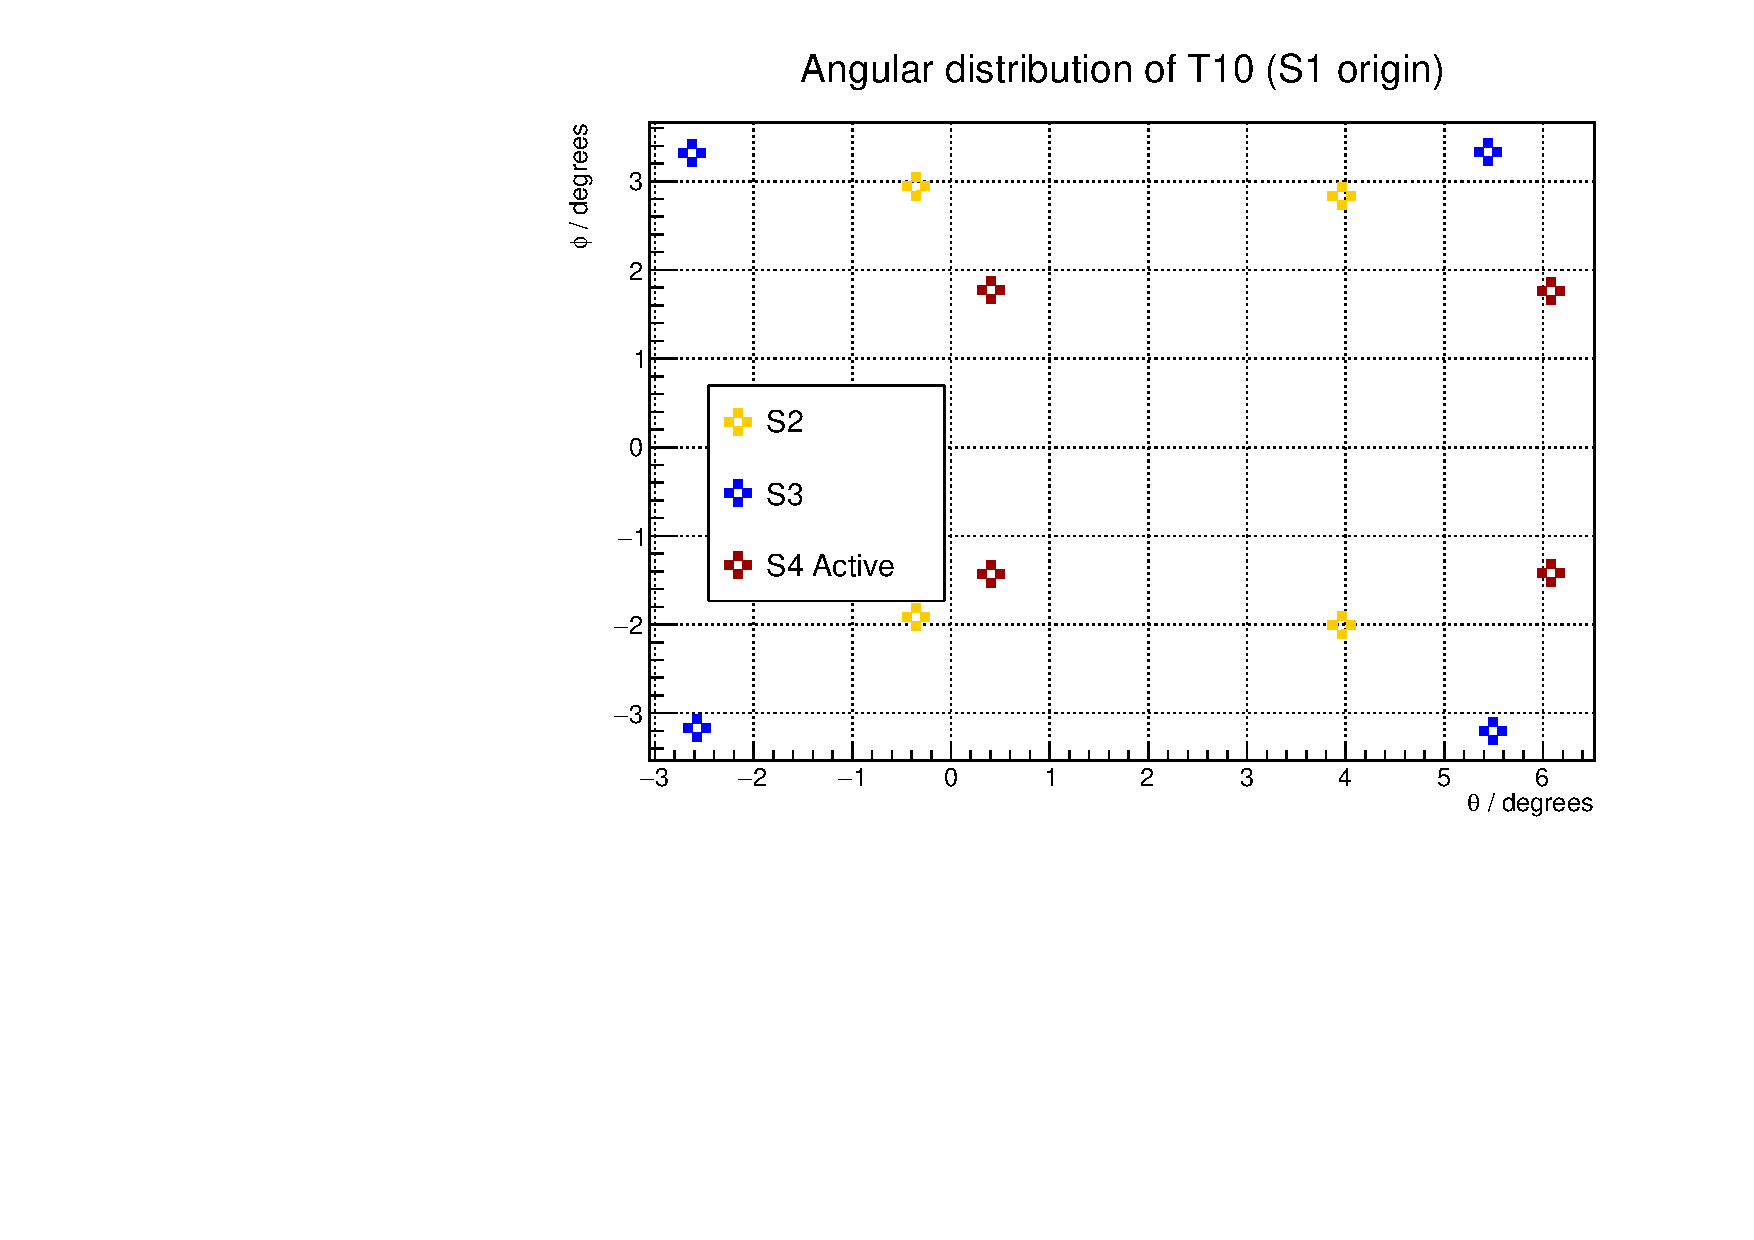
\includegraphics[width=\textwidth]{files/Figures/beamlineAng.pdf}
			\caption{Diagram showing the angular location of the extremities of the timing points. The coordinate system used has the origin at the $S1$ timing 	point, with the $x$ axis running parallel to the nominal axis.}
			\label{fig:beamAng}
		\end{minipage}
		\hspace{0.2cm}
		\begin{minipage}{0.49\textwidth}
			\begin{adjustbox}{max totalsize={\textwidth}{0.5\textheight}, center}
				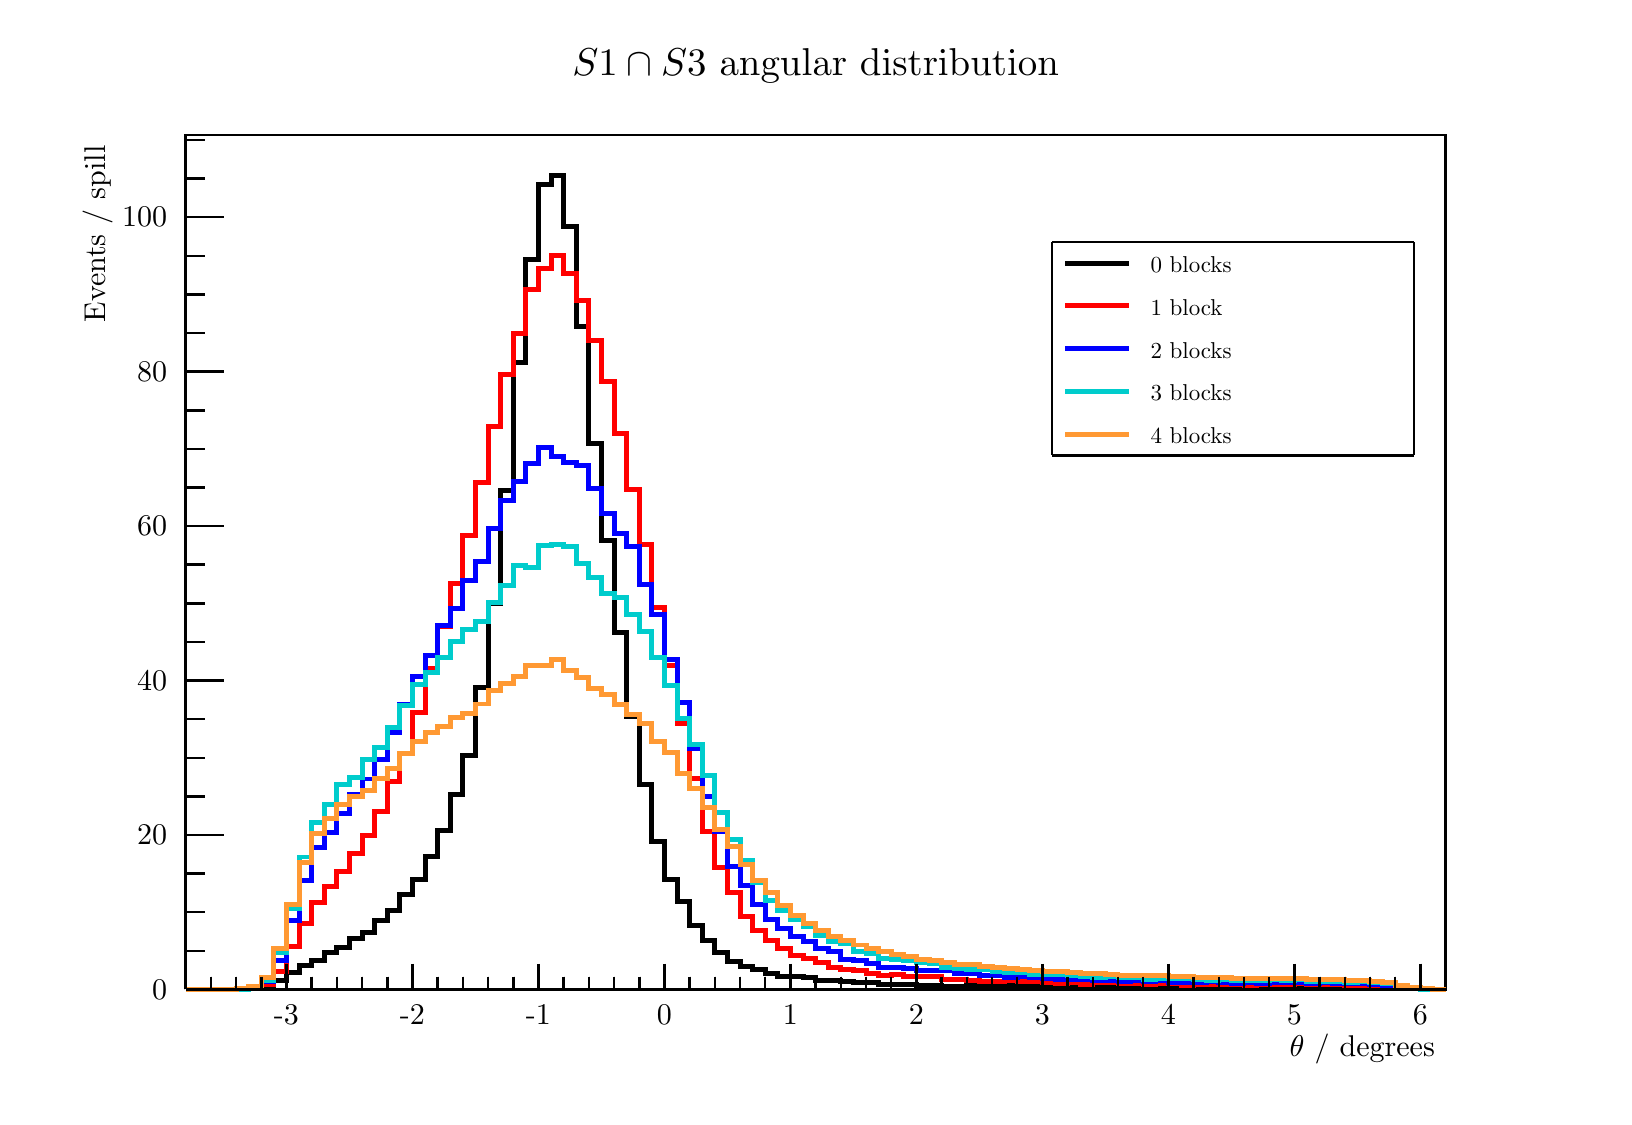
\begin{tikzpicture}
\pgfdeclareplotmark{cross} {
\pgfpathmoveto{\pgfpoint{-0.3\pgfplotmarksize}{\pgfplotmarksize}}
\pgfpathlineto{\pgfpoint{+0.3\pgfplotmarksize}{\pgfplotmarksize}}
\pgfpathlineto{\pgfpoint{+0.3\pgfplotmarksize}{0.3\pgfplotmarksize}}
\pgfpathlineto{\pgfpoint{+1\pgfplotmarksize}{0.3\pgfplotmarksize}}
\pgfpathlineto{\pgfpoint{+1\pgfplotmarksize}{-0.3\pgfplotmarksize}}
\pgfpathlineto{\pgfpoint{+0.3\pgfplotmarksize}{-0.3\pgfplotmarksize}}
\pgfpathlineto{\pgfpoint{+0.3\pgfplotmarksize}{-1.\pgfplotmarksize}}
\pgfpathlineto{\pgfpoint{-0.3\pgfplotmarksize}{-1.\pgfplotmarksize}}
\pgfpathlineto{\pgfpoint{-0.3\pgfplotmarksize}{-0.3\pgfplotmarksize}}
\pgfpathlineto{\pgfpoint{-1.\pgfplotmarksize}{-0.3\pgfplotmarksize}}
\pgfpathlineto{\pgfpoint{-1.\pgfplotmarksize}{0.3\pgfplotmarksize}}
\pgfpathlineto{\pgfpoint{-0.3\pgfplotmarksize}{0.3\pgfplotmarksize}}
\pgfpathclose
\pgfusepathqstroke
}
\pgfdeclareplotmark{cross*} {
\pgfpathmoveto{\pgfpoint{-0.3\pgfplotmarksize}{\pgfplotmarksize}}
\pgfpathlineto{\pgfpoint{+0.3\pgfplotmarksize}{\pgfplotmarksize}}
\pgfpathlineto{\pgfpoint{+0.3\pgfplotmarksize}{0.3\pgfplotmarksize}}
\pgfpathlineto{\pgfpoint{+1\pgfplotmarksize}{0.3\pgfplotmarksize}}
\pgfpathlineto{\pgfpoint{+1\pgfplotmarksize}{-0.3\pgfplotmarksize}}
\pgfpathlineto{\pgfpoint{+0.3\pgfplotmarksize}{-0.3\pgfplotmarksize}}
\pgfpathlineto{\pgfpoint{+0.3\pgfplotmarksize}{-1.\pgfplotmarksize}}
\pgfpathlineto{\pgfpoint{-0.3\pgfplotmarksize}{-1.\pgfplotmarksize}}
\pgfpathlineto{\pgfpoint{-0.3\pgfplotmarksize}{-0.3\pgfplotmarksize}}
\pgfpathlineto{\pgfpoint{-1.\pgfplotmarksize}{-0.3\pgfplotmarksize}}
\pgfpathlineto{\pgfpoint{-1.\pgfplotmarksize}{0.3\pgfplotmarksize}}
\pgfpathlineto{\pgfpoint{-0.3\pgfplotmarksize}{0.3\pgfplotmarksize}}
\pgfpathclose
\pgfusepathqfillstroke
}
\pgfdeclareplotmark{newstar} {
\pgfpathmoveto{\pgfqpoint{0pt}{\pgfplotmarksize}}
\pgfpathlineto{\pgfqpointpolar{44}{0.5\pgfplotmarksize}}
\pgfpathlineto{\pgfqpointpolar{18}{\pgfplotmarksize}}
\pgfpathlineto{\pgfqpointpolar{-20}{0.5\pgfplotmarksize}}
\pgfpathlineto{\pgfqpointpolar{-54}{\pgfplotmarksize}}
\pgfpathlineto{\pgfqpointpolar{-90}{0.5\pgfplotmarksize}}
\pgfpathlineto{\pgfqpointpolar{234}{\pgfplotmarksize}}
\pgfpathlineto{\pgfqpointpolar{198}{0.5\pgfplotmarksize}}
\pgfpathlineto{\pgfqpointpolar{162}{\pgfplotmarksize}}
\pgfpathlineto{\pgfqpointpolar{134}{0.5\pgfplotmarksize}}
\pgfpathclose
\pgfusepathqstroke
}
\pgfdeclareplotmark{newstar*} {
\pgfpathmoveto{\pgfqpoint{0pt}{\pgfplotmarksize}}
\pgfpathlineto{\pgfqpointpolar{44}{0.5\pgfplotmarksize}}
\pgfpathlineto{\pgfqpointpolar{18}{\pgfplotmarksize}}
\pgfpathlineto{\pgfqpointpolar{-20}{0.5\pgfplotmarksize}}
\pgfpathlineto{\pgfqpointpolar{-54}{\pgfplotmarksize}}
\pgfpathlineto{\pgfqpointpolar{-90}{0.5\pgfplotmarksize}}
\pgfpathlineto{\pgfqpointpolar{234}{\pgfplotmarksize}}
\pgfpathlineto{\pgfqpointpolar{198}{0.5\pgfplotmarksize}}
\pgfpathlineto{\pgfqpointpolar{162}{\pgfplotmarksize}}
\pgfpathlineto{\pgfqpointpolar{134}{0.5\pgfplotmarksize}}
\pgfpathclose
\pgfusepathqfillstroke
}
\definecolor{c}{rgb}{1,1,1};
\draw [color=c, fill=c] (0,0) rectangle (20,13.5632);
\draw [color=c, fill=c] (2,1.35632) rectangle (18,12.2069);
\definecolor{c}{rgb}{0,0,0};
\draw [c,line width=0.9] (2,1.35632) -- (2,12.2069) -- (18,12.2069) -- (18,1.35632) -- (2,1.35632);
\definecolor{c}{rgb}{1,1,1};
\draw [color=c, fill=c] (2,1.35632) rectangle (18,12.2069);
\definecolor{c}{rgb}{0,0,0};
\draw [c,line width=0.9] (2,1.35632) -- (2,12.2069) -- (18,12.2069) -- (18,1.35632) -- (2,1.35632);
\definecolor{c}{rgb}{0,0,0.6};
\draw [c,line width=0.9] (2,1.35632) -- (2.16,1.35632) -- (2.16,1.35632) -- (2.32,1.35632) -- (2.32,1.35632) -- (2.48,1.35632) -- (2.48,1.35632) -- (2.64,1.35632) -- (2.64,1.35632) -- (2.8,1.35632) -- (2.8,1.35632) -- (2.96,1.35632) -- (2.96,1.35632)
 -- (3.12,1.35632) -- (3.12,1.35632) -- (3.28,1.35632) -- (3.28,1.35632) -- (3.44,1.35632) -- (3.44,1.35632) -- (3.6,1.35632) -- (3.6,1.35632) -- (3.76,1.35632) -- (3.76,1.35632) -- (3.92,1.35632) -- (3.92,1.35632) -- (4.08,1.35632) -- (4.08,1.35632)
 -- (4.24,1.35632) -- (4.24,1.35632) -- (4.4,1.35632) -- (4.4,1.35632) -- (4.56,1.35632) -- (4.56,1.35632) -- (4.72,1.35632) -- (4.72,1.35632) -- (4.88,1.35632) -- (4.88,1.35632) -- (5.04,1.35632) -- (5.04,1.35632) -- (5.2,1.35632) -- (5.2,1.35632)
 -- (5.36,1.35632) -- (5.36,1.35632) -- (5.52,1.35632) -- (5.52,1.35632) -- (5.68,1.35632) -- (5.68,1.35632) -- (5.84,1.35632) -- (5.84,1.35632) -- (6,1.35632) -- (6,1.35632) -- (6.16,1.35632) -- (6.16,1.35632) -- (6.32,1.35632) -- (6.32,1.35632) --
 (6.48,1.35632) -- (6.48,1.35632) -- (6.64,1.35632) -- (6.64,1.35632) -- (6.8,1.35632) -- (6.8,1.35632) -- (6.96,1.35632) -- (6.96,1.35632) -- (7.12,1.35632) -- (7.12,1.35632) -- (7.28,1.35632) -- (7.28,1.35632) -- (7.44,1.35632) -- (7.44,1.35632) --
 (7.6,1.35632) -- (7.6,1.35632) -- (7.76,1.35632) -- (7.76,1.35632) -- (7.92,1.35632) -- (7.92,1.35632) -- (8.08,1.35632) -- (8.08,1.35632) -- (8.24,1.35632) -- (8.24,1.35632) -- (8.4,1.35632) -- (8.4,1.35632) -- (8.56,1.35632) -- (8.56,1.35632) --
 (8.72,1.35632) -- (8.72,1.35632) -- (8.88,1.35632) -- (8.88,1.35632) -- (9.04,1.35632) -- (9.04,1.35632) -- (9.2,1.35632) -- (9.2,1.35632) -- (9.36,1.35632) -- (9.36,1.35632) -- (9.52,1.35632) -- (9.52,1.35632) -- (9.68,1.35632) -- (9.68,1.35632) --
 (9.84,1.35632) -- (9.84,1.35632) -- (10,1.35632) -- (10,1.35632) -- (10.16,1.35632) -- (10.16,1.35632) -- (10.32,1.35632) -- (10.32,1.35632) -- (10.48,1.35632) -- (10.48,1.35632) -- (10.64,1.35632) -- (10.64,1.35632) -- (10.8,1.35632) --
 (10.8,1.35632) -- (10.96,1.35632) -- (10.96,1.35632) -- (11.12,1.35632) -- (11.12,1.35632) -- (11.28,1.35632) -- (11.28,1.35632) -- (11.44,1.35632) -- (11.44,1.35632) -- (11.6,1.35632) -- (11.6,1.35632) -- (11.76,1.35632) -- (11.76,1.35632) --
 (11.92,1.35632) -- (11.92,1.35632) -- (12.08,1.35632) -- (12.08,1.35632) -- (12.24,1.35632) -- (12.24,1.35632) -- (12.4,1.35632) -- (12.4,1.35632) -- (12.56,1.35632) -- (12.56,1.35632) -- (12.72,1.35632) -- (12.72,1.35632) -- (12.88,1.35632) --
 (12.88,1.35632) -- (13.04,1.35632) -- (13.04,1.35632) -- (13.2,1.35632) -- (13.2,1.35632) -- (13.36,1.35632) -- (13.36,1.35632) -- (13.52,1.35632) -- (13.52,1.35632) -- (13.68,1.35632) -- (13.68,1.35632) -- (13.84,1.35632) -- (13.84,1.35632) --
 (14,1.35632) -- (14,1.35632) -- (14.16,1.35632) -- (14.16,1.35632) -- (14.32,1.35632) -- (14.32,1.35632) -- (14.48,1.35632) -- (14.48,1.35632) -- (14.64,1.35632) -- (14.64,1.35632) -- (14.8,1.35632) -- (14.8,1.35632) -- (14.96,1.35632) --
 (14.96,1.35632) -- (15.12,1.35632) -- (15.12,1.35632) -- (15.28,1.35632) -- (15.28,1.35632) -- (15.44,1.35632) -- (15.44,1.35632) -- (15.6,1.35632) -- (15.6,1.35632) -- (15.76,1.35632) -- (15.76,1.35632) -- (15.92,1.35632) -- (15.92,1.35632) --
 (16.08,1.35632) -- (16.08,1.35632) -- (16.24,1.35632) -- (16.24,1.35632) -- (16.4,1.35632) -- (16.4,1.35632) -- (16.56,1.35632) -- (16.56,1.35632) -- (16.72,1.35632) -- (16.72,1.35632) -- (16.88,1.35632) -- (16.88,1.35632) -- (17.04,1.35632) --
 (17.04,1.35632) -- (17.2,1.35632) -- (17.2,1.35632) -- (17.36,1.35632) -- (17.36,1.35632) -- (17.52,1.35632) -- (17.52,1.35632) -- (17.68,1.35632) -- (17.68,1.35632) -- (17.84,1.35632) -- (17.84,1.35632) -- (18,1.35632);
\definecolor{c}{rgb}{0,0,0};
\draw [c,line width=0.9] (2,1.35632) -- (18,1.35632);
\draw [anchor= east] (18,0.596782) node[scale=1.08496, color=c, rotate=0]{$\theta$ / degrees};
\draw [c,line width=0.9] (3.28,1.68184) -- (3.28,1.35632);
\draw [c,line width=0.9] (3.6,1.51908) -- (3.6,1.35632);
\draw [c,line width=0.9] (3.92,1.51908) -- (3.92,1.35632);
\draw [c,line width=0.9] (4.24,1.51908) -- (4.24,1.35632);
\draw [c,line width=0.9] (4.56,1.51908) -- (4.56,1.35632);
\draw [c,line width=0.9] (4.88,1.68184) -- (4.88,1.35632);
\draw [c,line width=0.9] (5.2,1.51908) -- (5.2,1.35632);
\draw [c,line width=0.9] (5.52,1.51908) -- (5.52,1.35632);
\draw [c,line width=0.9] (5.84,1.51908) -- (5.84,1.35632);
\draw [c,line width=0.9] (6.16,1.51908) -- (6.16,1.35632);
\draw [c,line width=0.9] (6.48,1.68184) -- (6.48,1.35632);
\draw [c,line width=0.9] (6.8,1.51908) -- (6.8,1.35632);
\draw [c,line width=0.9] (7.12,1.51908) -- (7.12,1.35632);
\draw [c,line width=0.9] (7.44,1.51908) -- (7.44,1.35632);
\draw [c,line width=0.9] (7.76,1.51908) -- (7.76,1.35632);
\draw [c,line width=0.9] (8.08,1.68184) -- (8.08,1.35632);
\draw [c,line width=0.9] (8.4,1.51908) -- (8.4,1.35632);
\draw [c,line width=0.9] (8.72,1.51908) -- (8.72,1.35632);
\draw [c,line width=0.9] (9.04,1.51908) -- (9.04,1.35632);
\draw [c,line width=0.9] (9.36,1.51908) -- (9.36,1.35632);
\draw [c,line width=0.9] (9.68,1.68184) -- (9.68,1.35632);
\draw [c,line width=0.9] (10,1.51908) -- (10,1.35632);
\draw [c,line width=0.9] (10.32,1.51908) -- (10.32,1.35632);
\draw [c,line width=0.9] (10.64,1.51908) -- (10.64,1.35632);
\draw [c,line width=0.9] (10.96,1.51908) -- (10.96,1.35632);
\draw [c,line width=0.9] (11.28,1.68184) -- (11.28,1.35632);
\draw [c,line width=0.9] (11.6,1.51908) -- (11.6,1.35632);
\draw [c,line width=0.9] (11.92,1.51908) -- (11.92,1.35632);
\draw [c,line width=0.9] (12.24,1.51908) -- (12.24,1.35632);
\draw [c,line width=0.9] (12.56,1.51908) -- (12.56,1.35632);
\draw [c,line width=0.9] (12.88,1.68184) -- (12.88,1.35632);
\draw [c,line width=0.9] (13.2,1.51908) -- (13.2,1.35632);
\draw [c,line width=0.9] (13.52,1.51908) -- (13.52,1.35632);
\draw [c,line width=0.9] (13.84,1.51908) -- (13.84,1.35632);
\draw [c,line width=0.9] (14.16,1.51908) -- (14.16,1.35632);
\draw [c,line width=0.9] (14.48,1.68184) -- (14.48,1.35632);
\draw [c,line width=0.9] (14.8,1.51908) -- (14.8,1.35632);
\draw [c,line width=0.9] (15.12,1.51908) -- (15.12,1.35632);
\draw [c,line width=0.9] (15.44,1.51908) -- (15.44,1.35632);
\draw [c,line width=0.9] (15.76,1.51908) -- (15.76,1.35632);
\draw [c,line width=0.9] (16.08,1.68184) -- (16.08,1.35632);
\draw [c,line width=0.9] (16.4,1.51908) -- (16.4,1.35632);
\draw [c,line width=0.9] (16.72,1.51908) -- (16.72,1.35632);
\draw [c,line width=0.9] (17.04,1.51908) -- (17.04,1.35632);
\draw [c,line width=0.9] (17.36,1.51908) -- (17.36,1.35632);
\draw [c,line width=0.9] (17.68,1.68184) -- (17.68,1.35632);
\draw [c,line width=0.9] (3.28,1.68184) -- (3.28,1.35632);
\draw [c,line width=0.9] (2.96,1.51908) -- (2.96,1.35632);
\draw [c,line width=0.9] (2.64,1.51908) -- (2.64,1.35632);
\draw [c,line width=0.9] (2.32,1.51908) -- (2.32,1.35632);
\draw [c,line width=0.9] (17.68,1.68184) -- (17.68,1.35632);
\draw [anchor=base] (3.28,0.908736) node[scale=1.08496, color=c, rotate=0]{-3};
\draw [anchor=base] (4.88,0.908736) node[scale=1.08496, color=c, rotate=0]{-2};
\draw [anchor=base] (6.48,0.908736) node[scale=1.08496, color=c, rotate=0]{-1};
\draw [anchor=base] (8.08,0.908736) node[scale=1.08496, color=c, rotate=0]{0};
\draw [anchor=base] (9.68,0.908736) node[scale=1.08496, color=c, rotate=0]{1};
\draw [anchor=base] (11.28,0.908736) node[scale=1.08496, color=c, rotate=0]{2};
\draw [anchor=base] (12.88,0.908736) node[scale=1.08496, color=c, rotate=0]{3};
\draw [anchor=base] (14.48,0.908736) node[scale=1.08496, color=c, rotate=0]{4};
\draw [anchor=base] (16.08,0.908736) node[scale=1.08496, color=c, rotate=0]{5};
\draw [anchor=base] (17.68,0.908736) node[scale=1.08496, color=c, rotate=0]{6};
\draw [c,line width=0.9] (2,1.35632) -- (2,12.2069);
\draw [anchor= east] (0.88,12.2069) node[scale=1.08496, color=c, rotate=90]{ Events / spill};
\draw [c,line width=0.9] (2.48,1.35632) -- (2,1.35632);
\draw [c,line width=0.9] (2.24,1.84663) -- (2,1.84663);
\draw [c,line width=0.9] (2.24,2.33694) -- (2,2.33694);
\draw [c,line width=0.9] (2.24,2.82725) -- (2,2.82725);
\draw [c,line width=0.9] (2.48,3.31756) -- (2,3.31756);
\draw [c,line width=0.9] (2.24,3.80788) -- (2,3.80788);
\draw [c,line width=0.9] (2.24,4.29819) -- (2,4.29819);
\draw [c,line width=0.9] (2.24,4.7885) -- (2,4.7885);
\draw [c,line width=0.9] (2.48,5.27881) -- (2,5.27881);
\draw [c,line width=0.9] (2.24,5.76912) -- (2,5.76912);
\draw [c,line width=0.9] (2.24,6.25943) -- (2,6.25943);
\draw [c,line width=0.9] (2.24,6.74974) -- (2,6.74974);
\draw [c,line width=0.9] (2.48,7.24005) -- (2,7.24005);
\draw [c,line width=0.9] (2.24,7.73036) -- (2,7.73036);
\draw [c,line width=0.9] (2.24,8.22067) -- (2,8.22067);
\draw [c,line width=0.9] (2.24,8.71098) -- (2,8.71098);
\draw [c,line width=0.9] (2.48,9.20129) -- (2,9.20129);
\draw [c,line width=0.9] (2.24,9.6916) -- (2,9.6916);
\draw [c,line width=0.9] (2.24,10.1819) -- (2,10.1819);
\draw [c,line width=0.9] (2.24,10.6722) -- (2,10.6722);
\draw [c,line width=0.9] (2.48,11.1625) -- (2,11.1625);
\draw [c,line width=0.9] (2.48,11.1625) -- (2,11.1625);
\draw [c,line width=0.9] (2.24,11.6528) -- (2,11.6528);
\draw [c,line width=0.9] (2.24,12.1432) -- (2,12.1432);
\draw [anchor= east] (1.9,1.35632) node[scale=1.08496, color=c, rotate=0]{0};
\draw [anchor= east] (1.9,3.31756) node[scale=1.08496, color=c, rotate=0]{20};
\draw [anchor= east] (1.9,5.27881) node[scale=1.08496, color=c, rotate=0]{40};
\draw [anchor= east] (1.9,7.24005) node[scale=1.08496, color=c, rotate=0]{60};
\draw [anchor= east] (1.9,9.20129) node[scale=1.08496, color=c, rotate=0]{80};
\draw [anchor= east] (1.9,11.1625) node[scale=1.08496, color=c, rotate=0]{100};
\draw [c,line width=1.8] (2,1.35632) -- (2.16,1.35632) -- (2.16,1.35632) -- (2.32,1.35632) -- (2.32,1.35632) -- (2.48,1.35632) -- (2.48,1.35632) -- (2.64,1.35632) -- (2.64,1.35632) -- (2.8,1.35632) -- (2.8,1.36782) -- (2.96,1.36782) -- (2.96,1.39547)
 -- (3.12,1.39547) -- (3.12,1.46408) -- (3.28,1.46408) -- (3.28,1.5722) -- (3.44,1.5722) -- (3.44,1.66344) -- (3.6,1.66344) -- (3.6,1.7245) -- (3.76,1.7245) -- (3.76,1.83011) -- (3.92,1.83011) -- (3.92,1.88974) -- (4.08,1.88974) -- (4.08,1.99893) --
 (4.24,1.99893) -- (4.24,2.0758) -- (4.4,2.0758) -- (4.4,2.22631) -- (4.56,2.22631) -- (4.56,2.36029) -- (4.72,2.36029) -- (4.72,2.56432) -- (4.88,2.56432) -- (4.88,2.75182) -- (5.04,2.75182) -- (5.04,3.0478) -- (5.2,3.0478) -- (5.2,3.36929) --
 (5.36,3.36929) -- (5.36,3.82727) -- (5.52,3.82727) -- (5.52,4.32153) -- (5.68,4.32153) -- (5.68,5.18901) -- (5.84,5.18901) -- (5.84,6.25548) -- (6,6.25548) -- (6,7.69121) -- (6.16,7.69121) -- (6.16,9.31839) -- (6.32,9.31839) -- (6.32,10.6237) --
 (6.48,10.6237) -- (6.48,11.5792) -- (6.64,11.5792) -- (6.64,11.6902) -- (6.8,11.6902) -- (6.8,11.0411) -- (6.96,11.0411) -- (6.96,9.77386) -- (7.12,9.77386) -- (7.12,8.28461) -- (7.28,8.28461) -- (7.28,7.0626) -- (7.44,7.0626) -- (7.44,5.88622) --
 (7.6,5.88622) -- (7.6,4.82801) -- (7.76,4.82801) -- (7.76,3.95658) -- (7.92,3.95658) -- (7.92,3.23279) -- (8.08,3.23279) -- (8.08,2.75505) -- (8.24,2.75505) -- (8.24,2.47128) -- (8.4,2.47128) -- (8.4,2.17207) -- (8.56,2.17207) -- (8.56,1.98097) --
 (8.72,1.98097) -- (8.72,1.82652) -- (8.88,1.82652) -- (8.88,1.71516) -- (9.04,1.71516) -- (9.04,1.64584) -- (9.2,1.64584) -- (9.2,1.60992) -- (9.36,1.60992) -- (9.36,1.5546) -- (9.52,1.5546) -- (9.52,1.52227) -- (9.68,1.52227) -- (9.68,1.51796) --
 (9.84,1.51796) -- (9.84,1.50359) -- (10,1.50359) -- (10,1.46767) -- (10.16,1.46767) -- (10.16,1.46911) -- (10.32,1.46911) -- (10.32,1.45618) -- (10.48,1.45618) -- (10.48,1.44397) -- (10.64,1.44397) -- (10.64,1.44038) -- (10.8,1.44038) --
 (10.8,1.42349) -- (10.96,1.42349) -- (10.96,1.42457) -- (11.12,1.42457) -- (11.12,1.4181) -- (11.28,1.4181) -- (11.28,1.40877) -- (11.44,1.40877) -- (11.44,1.40661) -- (11.6,1.40661) -- (11.6,1.39547) -- (11.76,1.39547) -- (11.76,1.39763) --
 (11.92,1.39763) -- (11.92,1.40805) -- (12.08,1.40805) -- (12.08,1.40445) -- (12.24,1.40445) -- (12.24,1.39763) -- (12.4,1.39763) -- (12.4,1.40266) -- (12.56,1.40266) -- (12.56,1.40302) -- (12.72,1.40302) -- (12.72,1.38973) -- (12.88,1.38973) --
 (12.88,1.39224) -- (13.04,1.39224) -- (13.04,1.38362) -- (13.2,1.38362) -- (13.2,1.39152) -- (13.36,1.39152) -- (13.36,1.3926) -- (13.52,1.3926) -- (13.52,1.38901) -- (13.68,1.38901) -- (13.68,1.38614) -- (13.84,1.38614) -- (13.84,1.38721) --
 (14,1.38721) -- (14,1.38434) -- (14.16,1.38434) -- (14.16,1.38398) -- (14.32,1.38398) -- (14.32,1.38793) -- (14.48,1.38793) -- (14.48,1.38254) -- (14.64,1.38254) -- (14.64,1.38434) -- (14.8,1.38434) -- (14.8,1.38434) -- (14.96,1.38434) --
 (14.96,1.38183) -- (15.12,1.38183) -- (15.12,1.38829) -- (15.28,1.38829) -- (15.28,1.38326) -- (15.44,1.38326) -- (15.44,1.37536) -- (15.6,1.37536) -- (15.6,1.38757) -- (15.76,1.38757) -- (15.76,1.3829) -- (15.92,1.3829) -- (15.92,1.38039) --
 (16.08,1.38039) -- (16.08,1.38254) -- (16.24,1.38254) -- (16.24,1.38218) -- (16.4,1.38218) -- (16.4,1.37572) -- (16.56,1.37572) -- (16.56,1.38218) -- (16.72,1.38218) -- (16.72,1.37931) -- (16.88,1.37931) -- (16.88,1.3768) -- (17.04,1.3768) --
 (17.04,1.37716) -- (17.2,1.37716) -- (17.2,1.375) -- (17.36,1.375) -- (17.36,1.3653) -- (17.52,1.3653) -- (17.52,1.36315) -- (17.68,1.36315) -- (17.68,1.35848) -- (17.84,1.35848) -- (17.84,1.35632) -- (18,1.35632);
\definecolor{c}{rgb}{1,0,0};
\draw [c,line width=1.8] (2,1.35632) -- (2.16,1.35632) -- (2.16,1.35632) -- (2.32,1.35632) -- (2.32,1.35632) -- (2.48,1.35632) -- (2.48,1.35632) -- (2.64,1.35632) -- (2.64,1.35826) -- (2.8,1.35826) -- (2.8,1.36524) -- (2.96,1.36524) -- (2.96,1.41524)
 -- (3.12,1.41524) -- (3.12,1.58694) -- (3.28,1.58694) -- (3.28,1.89547) -- (3.44,1.89547) -- (3.44,2.18811) -- (3.6,2.18811) -- (3.6,2.45749) -- (3.76,2.45749) -- (3.76,2.66873) -- (3.92,2.66873) -- (3.92,2.85826) -- (4.08,2.85826) -- (4.08,3.08539)
 -- (4.24,3.08539) -- (4.24,3.30555) -- (4.4,3.30555) -- (4.4,3.61873) -- (4.56,3.61873) -- (4.56,3.99392) -- (4.72,3.99392) -- (4.72,4.35826) -- (4.88,4.35826) -- (4.88,4.87609) -- (5.04,4.87609) -- (5.04,5.42803) -- (5.2,5.42803) -- (5.2,5.96679)
 -- (5.36,5.96679) -- (5.36,6.50633) -- (5.52,6.50633) -- (5.52,7.11563) -- (5.68,7.11563) -- (5.68,7.79121) -- (5.84,7.79121) -- (5.84,8.51021) -- (6,8.51021) -- (6,9.16796) -- (6.16,9.16796) -- (6.16,9.6854) -- (6.32,9.6854) -- (6.32,10.2408) --
 (6.48,10.2408) -- (6.48,10.5067) -- (6.64,10.5067) -- (6.64,10.6823) -- (6.8,10.6823) -- (6.8,10.4428) -- (6.96,10.4428) -- (6.96,10.1087) -- (7.12,10.1087) -- (7.12,9.60168) -- (7.28,9.60168) -- (7.28,9.07571) -- (7.44,9.07571) -- (7.44,8.41873) --
 (7.6,8.41873) -- (7.6,7.7009) -- (7.76,7.7009) -- (7.76,7.01098) -- (7.92,7.01098) -- (7.92,6.20594) -- (8.08,6.20594) -- (8.08,5.46408) -- (8.24,5.46408) -- (8.24,4.72803) -- (8.4,4.72803) -- (8.4,4.03656) -- (8.56,4.03656) -- (8.56,3.3633) --
 (8.72,3.3633) -- (8.72,2.89935) -- (8.88,2.89935) -- (8.88,2.58113) -- (9.04,2.58113) -- (9.04,2.27919) -- (9.2,2.27919) -- (9.2,2.10787) -- (9.36,2.10787) -- (9.36,1.97997) -- (9.52,1.97997) -- (9.52,1.87105) -- (9.68,1.87105) -- (9.68,1.78539) --
 (9.84,1.78539) -- (9.84,1.74314) -- (10,1.74314) -- (10,1.70245) -- (10.16,1.70245) -- (10.16,1.63578) -- (10.32,1.63578) -- (10.32,1.60516) -- (10.48,1.60516) -- (10.48,1.59353) -- (10.64,1.59353) -- (10.64,1.56059) -- (10.8,1.56059) --
 (10.8,1.5288) -- (10.96,1.5288) -- (10.96,1.54159) -- (11.12,1.54159) -- (11.12,1.51873) -- (11.28,1.51873) -- (11.28,1.52376) -- (11.44,1.52376) -- (11.44,1.5164) -- (11.6,1.5164) -- (11.6,1.48074) -- (11.76,1.48074) -- (11.76,1.48113) --
 (11.92,1.48113) -- (11.92,1.46446) -- (12.08,1.46446) -- (12.08,1.45206) -- (12.24,1.45206) -- (12.24,1.45787) -- (12.4,1.45787) -- (12.4,1.46485) -- (12.56,1.46485) -- (12.56,1.45671) -- (12.72,1.45671) -- (12.72,1.45516) -- (12.88,1.45516) --
 (12.88,1.44043) -- (13.04,1.44043) -- (13.04,1.435) -- (13.2,1.435) -- (13.2,1.43966) -- (13.36,1.43966) -- (13.36,1.41795) -- (13.52,1.41795) -- (13.52,1.43888) -- (13.68,1.43888) -- (13.68,1.44198) -- (13.84,1.44198) -- (13.84,1.42764) --
 (14,1.42764) -- (14,1.42764) -- (14.16,1.42764) -- (14.16,1.41989) -- (14.32,1.41989) -- (14.32,1.43462) -- (14.48,1.43462) -- (14.48,1.43268) -- (14.64,1.43268) -- (14.64,1.40632) -- (14.8,1.40632) -- (14.8,1.41989) -- (14.96,1.41989) --
 (14.96,1.4164) -- (15.12,1.4164) -- (15.12,1.41911) -- (15.28,1.41911) -- (15.28,1.41407) -- (15.44,1.41407) -- (15.44,1.41175) -- (15.6,1.41175) -- (15.6,1.4133) -- (15.76,1.4133) -- (15.76,1.41446) -- (15.92,1.41446) -- (15.92,1.4164) --
 (16.08,1.4164) -- (16.08,1.42531) -- (16.24,1.42531) -- (16.24,1.41601) -- (16.4,1.41601) -- (16.4,1.41601) -- (16.56,1.41601) -- (16.56,1.41873) -- (16.72,1.41873) -- (16.72,1.40981) -- (16.88,1.40981) -- (16.88,1.40167) -- (17.04,1.40167) --
 (17.04,1.40012) -- (17.2,1.40012) -- (17.2,1.39198) -- (17.36,1.39198) -- (17.36,1.38074) -- (17.52,1.38074) -- (17.52,1.36407) -- (17.68,1.36407) -- (17.68,1.35904) -- (17.84,1.35904) -- (17.84,1.35787) -- (18,1.35787);
\definecolor{c}{rgb}{0,0,1};
\draw [c,line width=1.8] (2,1.35632) -- (2.16,1.35632) -- (2.16,1.35632) -- (2.32,1.35632) -- (2.32,1.35632) -- (2.48,1.35632) -- (2.48,1.35632) -- (2.64,1.35632) -- (2.64,1.35817) -- (2.8,1.35817) -- (2.8,1.37697) -- (2.96,1.37697) -- (2.96,1.4507)
 -- (3.12,1.4507) -- (3.12,1.7176) -- (3.28,1.7176) -- (3.28,2.22782) -- (3.44,2.22782) -- (3.44,2.74062) -- (3.6,2.74062) -- (3.6,3.1642) -- (3.76,3.1642) -- (3.76,3.34558) -- (3.92,3.34558) -- (3.92,3.59516) -- (4.08,3.59516) -- (4.08,3.83442) --
 (4.24,3.83442) -- (4.24,4.02833) -- (4.4,4.02833) -- (4.4,4.27865) -- (4.56,4.27865) -- (4.56,4.61449) -- (4.72,4.61449) -- (4.72,4.97577) -- (4.88,4.97577) -- (4.88,5.32415) -- (5.04,5.32415) -- (5.04,5.59659) -- (5.2,5.59659) -- (5.2,5.97409) --
 (5.36,5.97409) -- (5.36,6.19565) -- (5.52,6.19565) -- (5.52,6.5503) -- (5.68,6.5503) -- (5.68,6.78587) -- (5.84,6.78587) -- (5.84,7.21166) -- (6,7.21166) -- (6,7.56078) -- (6.16,7.56078) -- (6.16,7.80925) -- (6.32,7.80925) -- (6.32,8.03892) --
 (6.48,8.03892) -- (6.48,8.23247) -- (6.64,8.23247) -- (6.64,8.12703) -- (6.8,8.12703) -- (6.8,8.04961) -- (6.96,8.04961) -- (6.96,8.01091) -- (7.12,8.01091) -- (7.12,7.71451) -- (7.28,7.71451) -- (7.28,7.39488) -- (7.44,7.39488) -- (7.44,7.14973) --
 (7.6,7.14973) -- (7.6,6.98015) -- (7.76,6.98015) -- (7.76,6.49463) -- (7.92,6.49463) -- (7.92,6.12008) -- (8.08,6.12008) -- (8.08,5.54756) -- (8.24,5.54756) -- (8.24,5.00305) -- (8.4,5.00305) -- (8.4,4.41099) -- (8.56,4.41099) -- (8.56,3.80714) --
 (8.72,3.80714) -- (8.72,3.35959) -- (8.88,3.35959) -- (8.88,2.91942) -- (9.04,2.91942) -- (9.04,2.67205) -- (9.2,2.67205) -- (9.2,2.43501) -- (9.36,2.43501) -- (9.36,2.24183) -- (9.52,2.24183) -- (9.52,2.12386) -- (9.68,2.12386) -- (9.68,2.02322) --
 (9.84,2.02322) -- (9.84,1.96128) -- (10,1.96128) -- (10,1.87834) -- (10.16,1.87834) -- (10.16,1.83226) -- (10.32,1.83226) -- (10.32,1.73677) -- (10.48,1.73677) -- (10.48,1.7176) -- (10.64,1.7176) -- (10.64,1.68074) -- (10.8,1.68074) --
 (10.8,1.64055) -- (10.96,1.64055) -- (10.96,1.63834) -- (11.12,1.63834) -- (11.12,1.62028) -- (11.28,1.62028) -- (11.28,1.59374) -- (11.44,1.59374) -- (11.44,1.59447) -- (11.6,1.59447) -- (11.6,1.59079) -- (11.76,1.59079) -- (11.76,1.55429) --
 (11.92,1.55429) -- (11.92,1.55355) -- (12.08,1.55355) -- (12.08,1.53328) -- (12.24,1.53328) -- (12.24,1.53143) -- (12.4,1.53143) -- (12.4,1.50157) -- (12.56,1.50157) -- (12.56,1.51964) -- (12.72,1.51964) -- (12.72,1.50305) -- (12.88,1.50305) --
 (12.88,1.49236) -- (13.04,1.49236) -- (13.04,1.48535) -- (13.2,1.48535) -- (13.2,1.48535) -- (13.36,1.48535) -- (13.36,1.48314) -- (13.52,1.48314) -- (13.52,1.46618) -- (13.68,1.46618) -- (13.68,1.46692) -- (13.84,1.46692) -- (13.84,1.45807) --
 (14,1.45807) -- (14,1.46544) -- (14.16,1.46544) -- (14.16,1.45549) -- (14.32,1.45549) -- (14.32,1.46397) -- (14.48,1.46397) -- (14.48,1.44959) -- (14.64,1.44959) -- (14.64,1.4459) -- (14.8,1.4459) -- (14.8,1.44664) -- (14.96,1.44664) --
 (14.96,1.4507) -- (15.12,1.4507) -- (15.12,1.44922) -- (15.28,1.44922) -- (15.28,1.43706) -- (15.44,1.43706) -- (15.44,1.44443) -- (15.6,1.44443) -- (15.6,1.43521) -- (15.76,1.43521) -- (15.76,1.44406) -- (15.92,1.44406) -- (15.92,1.44443) --
 (16.08,1.44443) -- (16.08,1.44148) -- (16.24,1.44148) -- (16.24,1.43558) -- (16.4,1.43558) -- (16.4,1.44148) -- (16.56,1.44148) -- (16.56,1.43079) -- (16.72,1.43079) -- (16.72,1.43263) -- (16.88,1.43263) -- (16.88,1.42895) -- (17.04,1.42895) --
 (17.04,1.42305) -- (17.2,1.42305) -- (17.2,1.40535) -- (17.36,1.40535) -- (17.36,1.39098) -- (17.52,1.39098) -- (17.52,1.3648) -- (17.68,1.3648) -- (17.68,1.35964) -- (17.84,1.35964) -- (17.84,1.35743) -- (18,1.35743);
\definecolor{c}{rgb}{0,0.8,0.8};
\draw [c,line width=1.8] (2,1.35632) -- (2.16,1.35632) -- (2.16,1.35632) -- (2.32,1.35632) -- (2.32,1.35632) -- (2.48,1.35632) -- (2.48,1.35632) -- (2.64,1.35632) -- (2.64,1.35956) -- (2.8,1.35956) -- (2.8,1.38037) -- (2.96,1.38037) -- (2.96,1.46317)
 -- (3.12,1.46317) -- (3.12,1.82119) -- (3.28,1.82119) -- (3.28,2.38551) -- (3.44,2.38551) -- (3.44,3.03772) -- (3.6,3.03772) -- (3.6,3.4753) -- (3.76,3.4753) -- (3.76,3.70056) -- (3.92,3.70056) -- (3.92,3.96237) -- (4.08,3.96237) -- (4.08,4.04655)
 -- (4.24,4.04655) -- (4.24,4.27968) -- (4.4,4.27968) -- (4.4,4.43001) -- (4.56,4.43001) -- (4.56,4.68581) -- (4.72,4.68581) -- (4.72,4.96658) -- (4.88,4.96658) -- (4.88,5.2233) -- (5.04,5.2233) -- (5.04,5.37918) -- (5.2,5.37918) -- (5.2,5.56605) --
 (5.36,5.56605) -- (5.36,5.77883) -- (5.52,5.77883) -- (5.52,5.9324) -- (5.68,5.9324) -- (5.68,6.02306) -- (5.84,6.02306) -- (5.84,6.26683) -- (6,6.26683) -- (6,6.48608) -- (6.16,6.48608) -- (6.16,6.74558) -- (6.32,6.74558) -- (6.32,6.71875) --
 (6.48,6.71875) -- (6.48,6.99489) -- (6.64,6.99489) -- (6.64,7.006) -- (6.8,7.006) -- (6.8,6.98241) -- (6.96,6.98241) -- (6.96,6.76917) -- (7.12,6.76917) -- (7.12,6.58229) -- (7.28,6.58229) -- (7.28,6.38339) -- (7.44,6.38339) -- (7.44,6.32835) --
 (7.6,6.32835) -- (7.6,6.11187) -- (7.76,6.11187) -- (7.76,5.9028) -- (7.92,5.9028) -- (7.92,5.56559) -- (8.08,5.56559) -- (8.08,5.21775) -- (8.24,5.21775) -- (8.24,4.79081) -- (8.4,4.79081) -- (8.4,4.46239) -- (8.56,4.46239) -- (8.56,4.07847) --
 (8.72,4.07847) -- (8.72,3.59787) -- (8.88,3.59787) -- (8.88,3.2616) -- (9.04,3.2616) -- (9.04,2.98869) -- (9.2,2.98869) -- (9.2,2.71208) -- (9.36,2.71208) -- (9.36,2.4808) -- (9.52,2.4808) -- (9.52,2.35776) -- (9.68,2.35776) -- (9.68,2.24073) --
 (9.84,2.24073) -- (9.84,2.1547) -- (10,2.1547) -- (10,2.04322) -- (10.16,2.04322) -- (10.16,1.96088) -- (10.32,1.96088) -- (10.32,1.94469) -- (10.48,1.94469) -- (10.48,1.84154) -- (10.64,1.84154) -- (10.64,1.81333) -- (10.8,1.81333) --
 (10.8,1.74718) -- (10.96,1.74718) -- (10.96,1.73978) -- (11.12,1.73978) -- (11.12,1.72267) -- (11.28,1.72267) -- (11.28,1.69353) -- (11.44,1.69353) -- (11.44,1.68705) -- (11.6,1.68705) -- (11.6,1.63339) -- (11.76,1.63339) -- (11.76,1.61813) --
 (11.92,1.61813) -- (11.92,1.60703) -- (12.08,1.60703) -- (12.08,1.60842) -- (12.24,1.60842) -- (12.24,1.58853) -- (12.4,1.58853) -- (12.4,1.56771) -- (12.56,1.56771) -- (12.56,1.5728) -- (12.72,1.5728) -- (12.72,1.54782) -- (12.88,1.54782) --
 (12.88,1.54088) -- (13.04,1.54088) -- (13.04,1.54643) -- (13.2,1.54643) -- (13.2,1.53117) -- (13.36,1.53117) -- (13.36,1.52562) -- (13.52,1.52562) -- (13.52,1.50665) -- (13.68,1.50665) -- (13.68,1.5196) -- (13.84,1.5196) -- (13.84,1.51035) --
 (14,1.51035) -- (14,1.50388) -- (14.16,1.50388) -- (14.16,1.48769) -- (14.32,1.48769) -- (14.32,1.49555) -- (14.48,1.49555) -- (14.48,1.48908) -- (14.64,1.48908) -- (14.64,1.48954) -- (14.8,1.48954) -- (14.8,1.48723) -- (14.96,1.48723) --
 (14.96,1.47011) -- (15.12,1.47011) -- (15.12,1.47612) -- (15.28,1.47612) -- (15.28,1.46502) -- (15.44,1.46502) -- (15.44,1.47242) -- (15.6,1.47242) -- (15.6,1.46641) -- (15.76,1.46641) -- (15.76,1.48121) -- (15.92,1.48121) -- (15.92,1.4752) --
 (16.08,1.4752) -- (16.08,1.48445) -- (16.24,1.48445) -- (16.24,1.46086) -- (16.4,1.46086) -- (16.4,1.46271) -- (16.56,1.46271) -- (16.56,1.45531) -- (16.72,1.45531) -- (16.72,1.44883) -- (16.88,1.44883) -- (16.88,1.45901) -- (17.04,1.45901) --
 (17.04,1.4419) -- (17.2,1.4419) -- (17.2,1.42617) -- (17.36,1.42617) -- (17.36,1.39703) -- (17.52,1.39703) -- (17.52,1.37297) -- (17.68,1.37297) -- (17.68,1.35956) -- (17.84,1.35956) -- (17.84,1.35817) -- (18,1.35817);
\definecolor{c}{rgb}{1,0.6,0.2};
\draw [c,line width=1.8] (2,1.35632) -- (2.16,1.35632) -- (2.16,1.35632) -- (2.32,1.35632) -- (2.32,1.35632) -- (2.48,1.35632) -- (2.48,1.35799) -- (2.64,1.35799) -- (2.64,1.36238) -- (2.8,1.36238) -- (2.8,1.38719) -- (2.96,1.38719) -- (2.96,1.50637)
 -- (3.12,1.50637) -- (3.12,1.87937) -- (3.28,1.87937) -- (3.28,2.43978) -- (3.44,2.43978) -- (3.44,2.96208) -- (3.6,2.96208) -- (3.6,3.33819) -- (3.76,3.33819) -- (3.76,3.52264) -- (3.92,3.52264) -- (3.92,3.70999) -- (4.08,3.70999) -- (4.08,3.80033)
 -- (4.24,3.80033) -- (4.24,3.87923) -- (4.4,3.87923) -- (4.4,4.03815) -- (4.56,4.03815) -- (4.56,4.1584) -- (4.72,4.1584) -- (4.72,4.35363) -- (4.88,4.35363) -- (4.88,4.50688) -- (5.04,4.50688) -- (5.04,4.62293) -- (5.2,4.62293) -- (5.2,4.69959) --
 (5.36,4.69959) -- (5.36,4.80494) -- (5.52,4.80494) -- (5.52,4.86185) -- (5.68,4.86185) -- (5.68,4.98087) -- (5.84,4.98087) -- (5.84,5.14762) -- (6,5.14762) -- (6,5.24158) -- (6.16,5.24158) -- (6.16,5.33146) -- (6.32,5.33146) -- (6.32,5.47593) --
 (6.48,5.47593) -- (6.48,5.46903) -- (6.64,5.46903) -- (6.64,5.53977) -- (6.8,5.53977) -- (6.8,5.40817) -- (6.96,5.40817) -- (6.96,5.31578) -- (7.12,5.31578) -- (7.12,5.17474) -- (7.28,5.17474) -- (7.28,5.09762) -- (7.44,5.09762) -- (7.44,4.97125) --
 (7.6,4.97125) -- (7.6,4.84443) -- (7.76,4.84443) -- (7.76,4.73236) -- (7.92,4.73236) -- (7.92,4.50942) -- (8.08,4.50942) -- (8.08,4.36443) -- (8.24,4.36443) -- (8.24,4.10219) -- (8.4,4.10219) -- (8.4,3.90353) -- (8.56,3.90353) -- (8.56,3.66589) --
 (8.72,3.66589) -- (8.72,3.39243) -- (8.88,3.39243) -- (8.88,3.17668) -- (9.04,3.17668) -- (9.04,2.93725) -- (9.2,2.93725) -- (9.2,2.74328) -- (9.36,2.74328) -- (9.36,2.59231) -- (9.52,2.59231) -- (9.52,2.41628) -- (9.68,2.41628) -- (9.68,2.29479) --
 (9.84,2.29479) -- (9.84,2.19349) -- (10,2.19349) -- (10,2.10395) -- (10.16,2.10395) -- (10.16,2.02918) -- (10.32,2.02918) -- (10.32,1.97302) -- (10.48,1.97302) -- (10.48,1.92019) -- (10.64,1.92019) -- (10.64,1.87876) -- (10.8,1.87876) --
 (10.8,1.83873) -- (10.96,1.83873) -- (10.96,1.80394) -- (11.12,1.80394) -- (11.12,1.77128) -- (11.28,1.77128) -- (11.28,1.73826) -- (11.44,1.73826) -- (11.44,1.7194) -- (11.6,1.7194) -- (11.6,1.69728) -- (11.76,1.69728) -- (11.76,1.67668) --
 (11.92,1.67668) -- (11.92,1.66713) -- (12.08,1.66713) -- (12.08,1.64522) -- (12.24,1.64522) -- (12.24,1.63899) -- (12.4,1.63899) -- (12.4,1.62134) -- (12.56,1.62134) -- (12.56,1.60784) -- (12.72,1.60784) -- (12.72,1.59978) -- (12.88,1.59978) --
 (12.88,1.58696) -- (13.04,1.58696) -- (13.04,1.57756) -- (13.2,1.57756) -- (13.2,1.57025) -- (13.36,1.57025) -- (13.36,1.56148) -- (13.52,1.56148) -- (13.52,1.55717) -- (13.68,1.55717) -- (13.68,1.54498) -- (13.84,1.54498) -- (13.84,1.53862) --
 (14,1.53862) -- (14,1.53628) -- (14.16,1.53628) -- (14.16,1.53005) -- (14.32,1.53005) -- (14.32,1.52699) -- (14.48,1.52699) -- (14.48,1.52158) -- (14.64,1.52158) -- (14.64,1.51609) -- (14.8,1.51609) -- (14.8,1.51142) -- (14.96,1.51142) --
 (14.96,1.51142) -- (15.12,1.51142) -- (15.12,1.50472) -- (15.28,1.50472) -- (15.28,1.50003) -- (15.44,1.50003) -- (15.44,1.49785) -- (15.6,1.49785) -- (15.6,1.50093) -- (15.76,1.50093) -- (15.76,1.49898) -- (15.92,1.49898) -- (15.92,1.49277) --
 (16.08,1.49277) -- (16.08,1.49154) -- (16.24,1.49154) -- (16.24,1.4882) -- (16.4,1.4882) -- (16.4,1.48338) -- (16.56,1.48338) -- (16.56,1.47996) -- (16.72,1.47996) -- (16.72,1.47547) -- (16.88,1.47547) -- (16.88,1.47175) -- (17.04,1.47175) --
 (17.04,1.45792) -- (17.2,1.45792) -- (17.2,1.44071) -- (17.36,1.44071) -- (17.36,1.40664) -- (17.52,1.40664) -- (17.52,1.38111) -- (17.68,1.38111) -- (17.68,1.36363) -- (17.84,1.36363) -- (17.84,1.35837) -- (18,1.35837);
\definecolor{c}{rgb}{0,0,0};
\draw [c,line width=0.9] (2,1.35632) -- (18,1.35632);
\draw [c,line width=0.9] (3.28,1.68184) -- (3.28,1.35632);
\draw [c,line width=0.9] (3.6,1.51908) -- (3.6,1.35632);
\draw [c,line width=0.9] (3.92,1.51908) -- (3.92,1.35632);
\draw [c,line width=0.9] (4.24,1.51908) -- (4.24,1.35632);
\draw [c,line width=0.9] (4.56,1.51908) -- (4.56,1.35632);
\draw [c,line width=0.9] (4.88,1.68184) -- (4.88,1.35632);
\draw [c,line width=0.9] (5.2,1.51908) -- (5.2,1.35632);
\draw [c,line width=0.9] (5.52,1.51908) -- (5.52,1.35632);
\draw [c,line width=0.9] (5.84,1.51908) -- (5.84,1.35632);
\draw [c,line width=0.9] (6.16,1.51908) -- (6.16,1.35632);
\draw [c,line width=0.9] (6.48,1.68184) -- (6.48,1.35632);
\draw [c,line width=0.9] (6.8,1.51908) -- (6.8,1.35632);
\draw [c,line width=0.9] (7.12,1.51908) -- (7.12,1.35632);
\draw [c,line width=0.9] (7.44,1.51908) -- (7.44,1.35632);
\draw [c,line width=0.9] (7.76,1.51908) -- (7.76,1.35632);
\draw [c,line width=0.9] (8.08,1.68184) -- (8.08,1.35632);
\draw [c,line width=0.9] (8.4,1.51908) -- (8.4,1.35632);
\draw [c,line width=0.9] (8.72,1.51908) -- (8.72,1.35632);
\draw [c,line width=0.9] (9.04,1.51908) -- (9.04,1.35632);
\draw [c,line width=0.9] (9.36,1.51908) -- (9.36,1.35632);
\draw [c,line width=0.9] (9.68,1.68184) -- (9.68,1.35632);
\draw [c,line width=0.9] (10,1.51908) -- (10,1.35632);
\draw [c,line width=0.9] (10.32,1.51908) -- (10.32,1.35632);
\draw [c,line width=0.9] (10.64,1.51908) -- (10.64,1.35632);
\draw [c,line width=0.9] (10.96,1.51908) -- (10.96,1.35632);
\draw [c,line width=0.9] (11.28,1.68184) -- (11.28,1.35632);
\draw [c,line width=0.9] (11.6,1.51908) -- (11.6,1.35632);
\draw [c,line width=0.9] (11.92,1.51908) -- (11.92,1.35632);
\draw [c,line width=0.9] (12.24,1.51908) -- (12.24,1.35632);
\draw [c,line width=0.9] (12.56,1.51908) -- (12.56,1.35632);
\draw [c,line width=0.9] (12.88,1.68184) -- (12.88,1.35632);
\draw [c,line width=0.9] (13.2,1.51908) -- (13.2,1.35632);
\draw [c,line width=0.9] (13.52,1.51908) -- (13.52,1.35632);
\draw [c,line width=0.9] (13.84,1.51908) -- (13.84,1.35632);
\draw [c,line width=0.9] (14.16,1.51908) -- (14.16,1.35632);
\draw [c,line width=0.9] (14.48,1.68184) -- (14.48,1.35632);
\draw [c,line width=0.9] (14.8,1.51908) -- (14.8,1.35632);
\draw [c,line width=0.9] (15.12,1.51908) -- (15.12,1.35632);
\draw [c,line width=0.9] (15.44,1.51908) -- (15.44,1.35632);
\draw [c,line width=0.9] (15.76,1.51908) -- (15.76,1.35632);
\draw [c,line width=0.9] (16.08,1.68184) -- (16.08,1.35632);
\draw [c,line width=0.9] (16.4,1.51908) -- (16.4,1.35632);
\draw [c,line width=0.9] (16.72,1.51908) -- (16.72,1.35632);
\draw [c,line width=0.9] (17.04,1.51908) -- (17.04,1.35632);
\draw [c,line width=0.9] (17.36,1.51908) -- (17.36,1.35632);
\draw [c,line width=0.9] (17.68,1.68184) -- (17.68,1.35632);
\draw [c,line width=0.9] (3.28,1.68184) -- (3.28,1.35632);
\draw [c,line width=0.9] (2.96,1.51908) -- (2.96,1.35632);
\draw [c,line width=0.9] (2.64,1.51908) -- (2.64,1.35632);
\draw [c,line width=0.9] (2.32,1.51908) -- (2.32,1.35632);
\draw [c,line width=0.9] (17.68,1.68184) -- (17.68,1.35632);
\draw [c,line width=0.9] (2,1.35632) -- (2,12.2069);
\draw [c,line width=0.9] (2.48,1.35632) -- (2,1.35632);
\draw [c,line width=0.9] (2.24,1.84663) -- (2,1.84663);
\draw [c,line width=0.9] (2.24,2.33694) -- (2,2.33694);
\draw [c,line width=0.9] (2.24,2.82725) -- (2,2.82725);
\draw [c,line width=0.9] (2.48,3.31756) -- (2,3.31756);
\draw [c,line width=0.9] (2.24,3.80788) -- (2,3.80788);
\draw [c,line width=0.9] (2.24,4.29819) -- (2,4.29819);
\draw [c,line width=0.9] (2.24,4.7885) -- (2,4.7885);
\draw [c,line width=0.9] (2.48,5.27881) -- (2,5.27881);
\draw [c,line width=0.9] (2.24,5.76912) -- (2,5.76912);
\draw [c,line width=0.9] (2.24,6.25943) -- (2,6.25943);
\draw [c,line width=0.9] (2.24,6.74974) -- (2,6.74974);
\draw [c,line width=0.9] (2.48,7.24005) -- (2,7.24005);
\draw [c,line width=0.9] (2.24,7.73036) -- (2,7.73036);
\draw [c,line width=0.9] (2.24,8.22067) -- (2,8.22067);
\draw [c,line width=0.9] (2.24,8.71098) -- (2,8.71098);
\draw [c,line width=0.9] (2.48,9.20129) -- (2,9.20129);
\draw [c,line width=0.9] (2.24,9.6916) -- (2,9.6916);
\draw [c,line width=0.9] (2.24,10.1819) -- (2,10.1819);
\draw [c,line width=0.9] (2.24,10.6722) -- (2,10.6722);
\draw [c,line width=0.9] (2.48,11.1625) -- (2,11.1625);
\draw [c,line width=0.9] (2.48,11.1625) -- (2,11.1625);
\draw [c,line width=0.9] (2.24,11.6528) -- (2,11.6528);
\draw [c,line width=0.9] (2.24,12.1432) -- (2,12.1432);
\definecolor{c}{rgb}{1,1,1};
\draw [color=c, fill=c] (13,8.13793) rectangle (17.6,10.8506);
\definecolor{c}{rgb}{0,0,0};
\draw [c,line width=0.9] (13,8.13793) -- (17.6,8.13793);
\draw [c,line width=0.9] (17.6,8.13793) -- (17.6,10.8506);
\draw [c,line width=0.9] (17.6,10.8506) -- (13,10.8506);
\draw [c,line width=0.9] (13,10.8506) -- (13,8.13793);
\draw [anchor=base west] (14.15,10.4572) node[scale=0.829673, color=c, rotate=0]{0 blocks};
\draw [c,line width=1.8] (13.1725,10.5793) -- (13.9775,10.5793);
\draw [anchor=base west] (14.15,9.91471) node[scale=0.829673, color=c, rotate=0]{1 block};
\definecolor{c}{rgb}{1,0,0};
\draw [c,line width=1.8] (13.1725,10.0368) -- (13.9775,10.0368);
\definecolor{c}{rgb}{0,0,0};
\draw [anchor=base west] (14.15,9.37218) node[scale=0.829673, color=c, rotate=0]{2 blocks};
\definecolor{c}{rgb}{0,0,1};
\draw [c,line width=1.8] (13.1725,9.49425) -- (13.9775,9.49425);
\definecolor{c}{rgb}{0,0,0};
\draw [anchor=base west] (14.15,8.82965) node[scale=0.829673, color=c, rotate=0]{3 blocks};
\definecolor{c}{rgb}{0,0.8,0.8};
\draw [c,line width=1.8] (13.1725,8.95172) -- (13.9775,8.95172);
\definecolor{c}{rgb}{0,0,0};
\draw [anchor=base west] (14.15,8.28713) node[scale=0.829673, color=c, rotate=0]{4 blocks};
\definecolor{c}{rgb}{1,0.6,0.2};
\draw [c,line width=1.8] (13.1725,8.40919) -- (13.9775,8.40919);
\definecolor{c}{rgb}{0,0,0};
\draw (10,13.0816) node[scale=1.40406, color=c, rotate=0]{$S1 \cap S3$ angular distribution};
\end{tikzpicture}

			\end{adjustbox}
			\caption{Total particle flux passing through $S1$ and $S3$ for various numbers of moderator blocks. The flux is shown as a function of the off-axis angle in the $x-y$ plane with the origin at $S1$ and the $x$ axis running parallel to the nominal beamline.}
			\label{fig:s1s3all}
		\end{minipage}
		\
	\end{figure}
		
	\begin{table}
		\centering
		\begin{tabular}{|c|c|c|c|c|}
			\hline
			Number of blocks & $S3$ int. & $S2$ int. & $S2 \cap S4$ int. & $S4$ int. \\
			\hline
			0 & 1 & 0.1596 & 0.02074 & 0.02287 \\
			1 & 1 & 0.2480 & 0.04051 & 0.04362 \\
			2 & 1 & 0.2741 & 0.05943 & 0.06385 \\
			3 & 1 & 0.2893 & 0.07760 & 0.08423 \\
			4 & 1 & 0.3025 & 0.09816 & 0.1079  \\
			\hline		
		\end{tabular}
		\caption{Table showing the calculated flux corrections for various numbers of moderator blocks.}
		\label{tab:fluxFactors}
	\end{table}
	